\bookpart{概率图模型}{Probabilistic Graphical Models}
\label{part:probabilistic-models}

\BookPartGuide{%
本部分研究怎样用局部概率关系组织复杂联合分布，并根据观测回答查询。图规定哪些变量进入同一个局部函数，概率函数给出数值；一个完整配置容易评价，并不意味着汇总大量未观测状态同样容易。

第\ref{chap:pgm-overview}章建立表示、推断和学习的分工。有向图、无向图及不同表示的比较说明图能编码什么独立关系；变量消除和团树重组精确计算，变分与采样则在可承受的预算内近似查询。参数学习与结构学习分别处理局部函数未知和依赖连接未知的情形，缺失观测与潜变量贯穿其中。

后面的典型模型把这些工具落到静态有向模型、能量模型、动态模型与神经生成模型中。图的概率语义、推断算法和神经参数化是不同层面的选择；采用更灵活的局部函数，不会自动消除归一化、可识别性与推断成本。}

\chapter{概率图模型概述}
\label{chap:pgm-overview}

一台设备发出报警，维修人员需要判断是否停机检查。设备故障造成的过热和传感器失灵都可能触发报警，因此同一条报警记录可以对应不同的内部状态。判断“有故障”之外，还需要估计故障发生的概率，并结合后续温度读数更新判断。故障概率为$0.02$与$0.45$时，即使模型给出同一个分类结果，停机决策所依据的风险也不同。

设备诊断因而需要一个同时描述故障、温度与报警的分布。\term{概率图模型}（probabilistic graphical model, PGM）将这些随机变量画成节点，用图组织局部依赖，再由局部概率函数组成联合分布。可信的局部依赖假设可以减少需要指定的概率，也为复用计算提供依据。本章沿着设备诊断展开：先说明分布保留了哪些预测信息，再建立图与联合分布的关系，最后区分根据证据查询概率和根据数据确定模型这两类任务。

\section{从单值预测到结构化分布}
\label{sec:pgm-overview-distribution-prediction}

以传感器读数$x$预测设备下一时刻的温度时，模型可以返回$\hat y=f(x)$。这种\term{点预测}（point prediction）用一个数值概括输出，分类任务则用一个类别概括输出。它能直接进入后续决策，但单个结果中包含的信息有限，例如一个温度均值没有说明高温状态出现的概率。

保留这些信息的一种方式是给出\term{预测分布}（predictive distribution）$p(y\mid x)$，描述输入固定后各个输出的可能性。离散输出由每种结果的概率表示，连续输出由概率密度表示，落入某个区间的概率通过积分得到。分布可以同时呈现结果的集中位置、分散程度和多个分离的高概率区域。

图~\ref{fig:pgm-overview-predictive-density}用一个人工设定的温度分布说明这种区别。冷却系统有两种可能工况，预测密度分别集中在$40\,^\circ\mathrm{C}$和$80\,^\circ\mathrm{C}$附近，权重各为一半。两种工况的平均温度是$60\,^\circ\mathrm{C}$，恰好落在两个峰之间的低密度区域。保留完整分布能够同时呈现高温和低温工况；用均值或其中一个峰作点预测，则分别丢失峰的位置或另一种工况的信息。

\begin{figure}[htbp]
  \centering
  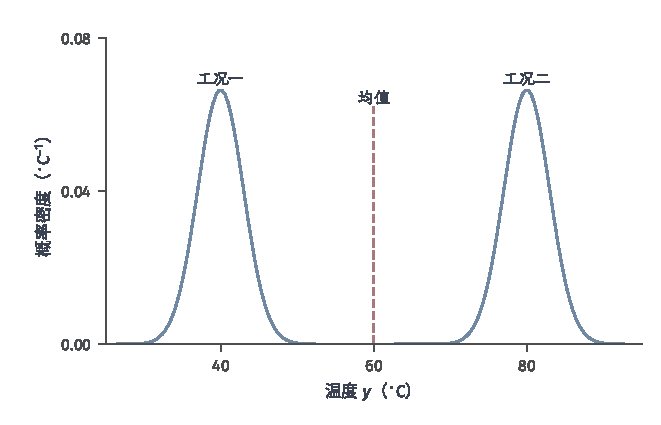
\includegraphics[width=105.412mm]{figures/06-probabilistic-graphical-models/01-representation/matplotlib/pgm-overview-predictive-density/figure.pdf}
  \caption{温度预测中的双峰分布与均值。实线为两个等权高斯密度的混合，每个分量的标准差为$3\,^\circ\mathrm{C}$；虚线标出均值$60\,^\circ\mathrm{C}$。两种工况集中在均值两侧，因而均值这一点预测省略了高概率区域的位置。图中分布为教学设定。}
  \label{fig:pgm-overview-predictive-density}
\end{figure}

预测分布也可以用来产生点预测。设备控制需要一个温度设定值时，可以从分布中选择均值；判断最可能工况时，可以选择概率最大的结果；停机决策则需要把可能的损失一并考虑。分布保留输出的不确定性，具体任务决定怎样将这些信息转化为数值、类别或行动。

当设备包含多个相互影响的部件时，预测还需要联合描述它们的状态。$d$个二值变量共有$2^d$种状态组合，直接指定完整联合表需要$2^d-1$个自由参数。变量数量增加会使数据分散在更多组合中，边缘概率的计算也可能涉及大量状态的汇总。利用局部依赖组织联合分布，正是为了在假设允许的范围内减少参数和计算。

故障与报警之间的联系必须保留，因而把所有变量设为相互独立会损失诊断所需的信息。局部简化可以更有针对性：假设报警只直接依赖过热和传感器失灵，那么给定这两个状态后，故障状态便不再改变报警的局部概率。这种“给定哪些状态后，另一个状态不再提供额外信息”的关系由条件独立表达，并由图结构记录。

\section{图模型上的表示}
\label{sec:pgm-overview-representation}
\label{sec:pgm-overview-basic-concepts}

设备诊断需要同时记录故障、过热、报警和传感器状态。画成图以后，读者不仅要知道哪些状态有关，还要分清哪些量已经观测、哪些量需要推断，以及哪些数值只是模型给定的参数。本节参考PRML第8章的图表示约定，用同一个设备例子说明节点、连线和重复框的含义\scite{bishop2006}。

\paragraph{随机变量与观测状态}
为设备的四种状态分别引入二值随机变量：故障$F$、过热$H$、报警$A$和传感器失灵$S$。每个变量取值$1$表示相应事件发生，取值$0$表示未发生。大写字母表示随机变量，小写$f,h,a,s\in\{0,1\}$表示它们的具体取值；因此$p(f,h,a,s)$是$F=f,H=h,A=a,S=s$同时成立的概率。

圆圈表示随机变量，圈内写变量名称。节点也可以代表一个随机向量，例如把四种状态合为$\bm V=(F,H,A,S)$，图中便可只画一个标有$\bm V$的圆圈。图~\ref{fig:pgm-overview-node-granularity}比较这两种粒度：圆圈的数量并不一定等于标量分量的数量。对于当前尚未取得取值的变量，节点保持空心；已经观测到的变量则给圆圈填色。只有报警记录$A=1$时，$A$画成填色圆圈，$F,H,S$仍为空心。若随后测得过热状态，$H$也改为填色，但模型中的依赖关系不必因此改变。图~\ref{fig:pgm-overview-visual-conventions}对照这两个观测条件，连线保持不变，变化的是节点的填色。

\begin{figure}[!htb]
  \centering
  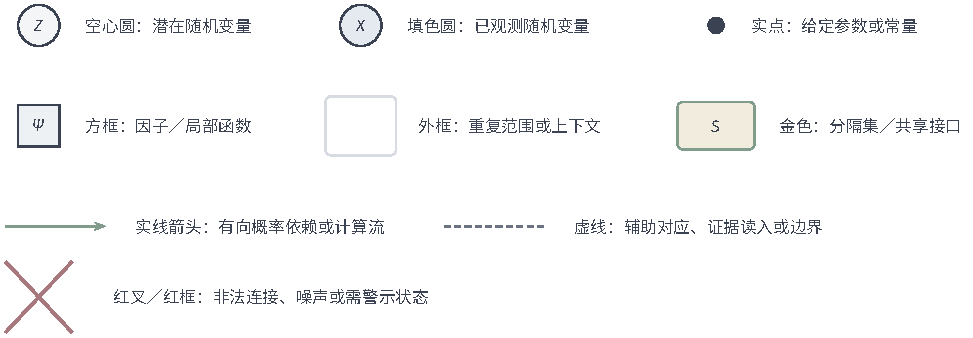
\includegraphics[width=77.646mm]{figures/06-probabilistic-graphical-models/01-representation/tikz/pgm-overview-visual-conventions/figure.pdf}
  \caption{观测信息改变节点填色。(a)仅知报警$A=1$；(b)又测得过热$H=1$。两图使用相同的变量与连线，故障和传感器状态仍未观测；填色表示已有取值，不表示删除随机变量。}
  \label{fig:pgm-overview-visual-conventions}
\end{figure}
\FloatBarrier

\begin{figure}[!htb]
  \centering
  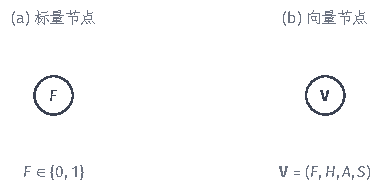
\includegraphics[width=64.703mm]{figures/06-probabilistic-graphical-models/01-representation/tikz/pgm-overview-node-granularity/figure.pdf}
  \caption{圆圈可以表示不同粒度的随机量。(a)一个故障状态$F$；(b)由四种状态组成的随机向量$\bm V$。向量节点并没有把四个分量变成同一个标量，也不表明各分量独立。}
  \label{fig:pgm-overview-node-granularity}
\end{figure}
\FloatBarrier

填色说明这次查询已知什么，不改变变量原本的随机性。空心也不专指模型主动引入的潜变量：尚未观测的故障是当前诊断目标，未来尚未产生的报警也可以是预测目标。对当前记录，模型引入而没有直接观测的内部状态称为潜变量；哪些节点已知、哪些未知，应结合观测条件来读。

只有报警已知而要判断故障时，必须先汇总过热和传感器失灵的可能取值，再按报警概率归一化：
\begin{equation}
  p(f,a)=\sum_{h,s}p(f,h,a,s),
  \qquad
  p(f\mid a)=\frac{p(f,a)}{p(a)},\quad p(a)>0.
  \label{eq:pgm-overview-marginal-conditional}
\end{equation}
这里$\sum_{h,s}$遍历$h,s\in\{0,1\}$的四种组合，$p(a)=\sum_f p(f,a)$；竖线右侧的$a$是已经给定的报警取值。第一式得到故障与报警的边缘概率，第二式使给定报警后故障两种取值的概率之和为$1$。连续变量用相应积分消去，条件分布的基本约定见\BookSectionRef{sec:rv-conditional-distribution}{卷2《数学准备：概率、因果与决策》第1章“随机变量”第1.2.2.2节“条件信息下的分布关系”}。

\paragraph{有向边与局部条件分布}
节点说明模型包含哪些量，连线则组织这些量之间的关系。先不省略任何条件，链式法则给出
\[
  p(f,s,h,a)=p(f)p(s\mid f)p(h\mid f,s)p(a\mid f,s,h).
\]
每一项都保留之前变量的全部取值，因此这种写法并没有减少完整联合表所需的参数。只有进一步指定条件独立关系，才能删去不需要的条件。

条件独立记为$X\perp Y\mid W$，其中$X,Y,W$是随机变量，$x,y,w$是它们各自的取值：给定$W$后，再知道$Y$不会改变$X$的条件分布。对本节的离散变量，在$p(y,w)>0$时可写为$p(x\mid y,w)=p(x\mid w)$；一般条件分布的等式按条件变量的分布几乎处处成立。当前需要的是这些关系怎样简化局部函数，通用独立性约定可参考\BookSectionRef{sec:probability-moments-independence}{卷2《数学准备：概率、因果与决策》第1章“随机变量”第1.2.3节“随机变量的独立关系”}。

设备模型假设故障与传感器失灵独立，过热在给定故障后不再依赖传感器状态，报警在给定过热与传感器状态后不再依赖故障。由此将链式分解中的相应条件删去，得到
\begin{equation}
  p(f,h,a,s)=p(f)p(s)p(h\mid f)p(a\mid h,s).
  \label{eq:pgm-overview-device-joint}
\end{equation}
每个局部条件分布对输出变量归一化，这个乘积就定义了完整联合分布。二值根变量$F,S$各需一个参数；$H$在$F$的两个取值下各需一个参数；$A$在$(H,S)$的四种组合下各需一个参数。总计$8$个自由参数，而完整联合表需要$15$个；减少的参数来自这里采用的独立性假设。

\term{有向图模型}（directed graphical model）用箭头指定局部条件分布使用哪些父变量。进入$A$的两条边$H\to A\leftarrow S$对应$p(a\mid h,s)$；$F\to H$对应$p(h\mid f)$；没有进入$F,S$的边，所以它们分别使用$p(f),p(s)$。图~\ref{fig:pgm-overview-device-graph}画出这一对应。箭头先表示概率分解中的条件关系，因果解释需要额外假设；它也不表示算法必须按箭头方向传递查询信息。第~\ref{chap:pgm-directed}章进一步说明有向分解与条件独立的对应。



\begin{figure}[!htb]
  \centering
  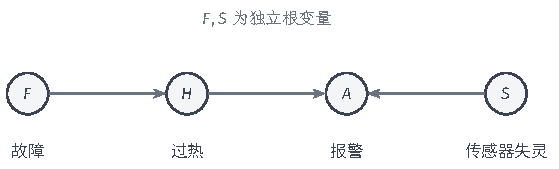
\includegraphics[width=94.590mm]{figures/06-probabilistic-graphical-models/01-representation/tikz/pgm-overview-device-graph/figure.pdf}
  \caption{设备诊断的有向表示。节点表示随机变量，进入节点的箭头指定其局部条件分布所依赖的变量，例如$H\to A\leftarrow S$对应$p(a\mid h,s)$。这里的箭头记录概率分解，因果解释需要另行给出假设。}
  \label{fig:pgm-overview-device-graph}
\end{figure}

\FloatBarrier

\paragraph{固定量与参数节点}
图规定局部函数可以使用哪些变量，函数中的数值还需另外指定。例如，令$\bm\theta_A$收集四种$(h,s)$组合下的报警概率$p(A=1\mid H=h,S=s)$。查询故障时，若这张概率表已经给定，$\bm\theta_A$就是固定量，可以画成小实点，再连到使用它的报警节点。图~\ref{fig:pgm-overview-parameter-roles}(a)只保留报警与其固定参数，显示小实点的作用。

填色大圆圈与小实点承担不同职责：前者是模型中的随机变量，只是本次已经取得取值；后者在当前概率模型中作为给定量使用，不需要对它建立概率分布。固定输入也可以用小实点表示，例如回归中给定的输入位置。参数是否画成实点取决于建模方式，而不是它被称为“参数”：若要为参数本身指定先验并推断其分布，就应将它画成随机变量圆圈。图~\ref{fig:pgm-overview-parameter-roles}(b)用$\bm\Theta_A$表示随机参数，$\bm\theta_A$仍表示它的一种取值。具体参数学习方式由第~\ref{chap:pgm-parameter-learning}章介绍。

\begin{figure}[!htb]
  \centering
  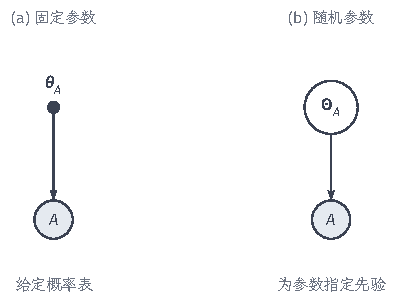
\includegraphics[width=67.165mm]{figures/06-probabilistic-graphical-models/01-representation/tikz/pgm-overview-parameter-roles/figure.pdf}
  \caption{同一参数的两种建模方式。左图将报警表作为固定量，右图为参数$\bm\Theta_A$指定先验，使用随机变量圆圈。两图都观测报警$A$，均省略$H,S$及其入$A$的箭头；实点与填色圆圈不是同一类对象。}
  \label{fig:pgm-overview-parameter-roles}
\end{figure}
\FloatBarrier

同一张图配上不同的局部概率表，会给出不同的诊断结果。图结构组织允许的依赖，参数与局部函数确定具体概率；为保持图简洁，已经在正文说明的固定参数可以不全部画出。

\paragraph{重复框与共享参数}
多台设备采用相同诊断模型时，每条记录都有自己的$F_i,H_i,A_i,S_i$。若逐条画出，节点和连接会大量重复。\term{板表示法}（plate notation）用一个框圈住代表性节点及其连接，再用$N$标出重复次数；下标$i=1,\ldots,N$说明框内变量按记录复制。图~\ref{fig:pgm-overview-plate-expansion}取$N=3$对照展开图和板框图，只保留过热、传感器失灵与报警这三个节点；省略的故障节点也随记录复制。框外的$\bm\theta_A$不复制，而是由每套报警节点共同使用。

\begin{figure*}[!htb]
  \centering
  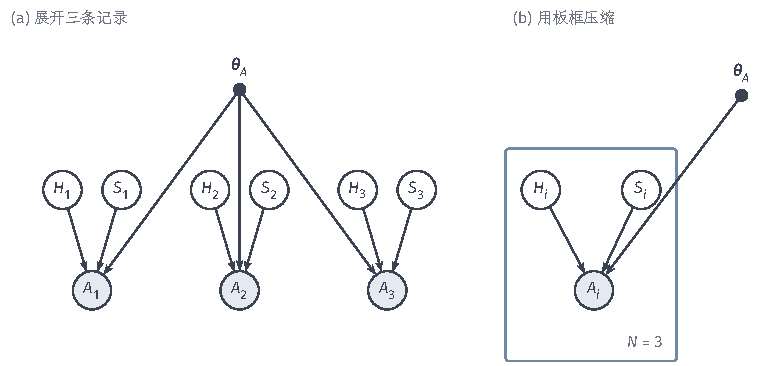
\includegraphics[width=128.926mm]{figures/06-probabilistic-graphical-models/01-representation/tikz/pgm-overview-plate-expansion/figure.pdf}
  \caption{重复框与展开图，取三条记录作图示。左图有三个过热、三个传感器和三个报警变量，三组报警共用一个固定参数；右图用$N=3$的板框压缩这些副本。两图均省略故障变量及相关箭头，框外参数不随记录复制。}
  \label{fig:pgm-overview-plate-expansion}
\end{figure*}
\FloatBarrier

若各记录在给定整组固定参数$\bm\theta$后相互独立，用$p_{\bm\theta}$表示采用这组参数的分布，则重复图对应的联合概率为
\begin{equation}
  p_{\bm\theta}(f_{1:N},h_{1:N},a_{1:N},s_{1:N})
    =\prod_{i=1}^{N}p_{\bm\theta}(f_i,h_i,a_i,s_i).
  \label{eq:pgm-overview-plate-product}
\end{equation}
$\bm\theta$包含四类局部概率表的全部参数，$f_{1:N}$表示$f_1,\ldots,f_N$，其余下标同理。每条记录使用相同的函数形式和参数，但保留自己的状态取值。框本身只表示重复，不单独保证记录独立；若副本之间另有连接，或共享的随机量被边缘化，就要按展开后的依赖关系计算联合分布。

\paragraph{无向边与因子节点}
若重点是邻近部件状态之间的对称相互作用，可以使用\term{无向图模型}（undirected graphical model）。无向边没有箭头，不指定哪个端点作为另一个端点的条件；局部关系由非负势函数评价配置的相对权重。令$\bm x$为全部变量的取值，$c$为局部作用范围的索引，$\bm x_c$为该范围内的取值子向量，则
\[
  p(\bm x)=\frac{1}{Z}\prod_c\psi_c(\bm x_c),
  \qquad
  Z=\sum_{\bm x}\prod_c\psi_c(\bm x_c).
\]
$\psi_c\geq0$是局部势，$Z$是对全部候选配置求和的归一化常数。离散情形下$p(\bm x)$表示联合概率，连续情形下表示密度；连续状态改用积分，且须满足$0<Z<\infty$。无向边表示模型允许的局部相互作用，不等同于两个变量的边缘相关系数。其条件独立语义在第~\ref{chap:pgm-undirected}章展开。

局部函数也可以单独画出来。\term{因子图}（factor graph）用圆圈表示变量、方框表示因子，连接线说明函数用到了哪些变量。例如，令$g_A(a,h,s)=p(a\mid h,s)$，相应的$g_A$方框连接$A,H,S$。这三条无箭头连线表示函数的三个自变量，并不是新增三条随机变量之间的无向边；$g_A$也不需要被观测或赋予一个随机取值。图~\ref{fig:pgm-overview-edge-types}进一步对照无向变量边和一个三变量因子的连线：左图直接连接变量，右图把局部函数单独画出。

\begin{figure}[!htb]
  \centering
  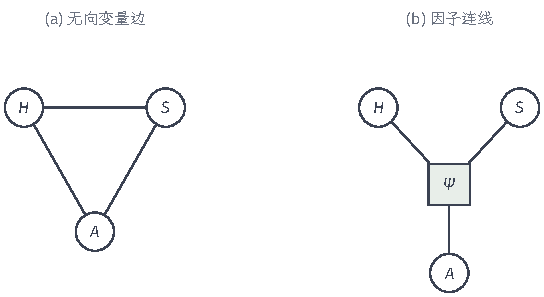
\includegraphics[width=92.135mm]{figures/06-probabilistic-graphical-models/01-representation/tikz/pgm-overview-edge-types/figure.pdf}
  \caption{无向边与变量—因子连线的对象不同。左图允许$H,S,A$组成一个三变量局部作用范围，右图将该范围的势函数$\psi(h,s,a)$显式画成方框。右图的每条线连接一个变量和一个函数，不能读成新增的变量之间连线；两图均不标注观测证据。}
  \label{fig:pgm-overview-edge-types}
\end{figure}
\FloatBarrier

有向模型的条件概率乘积和无向模型的势函数乘积都能画成因子图。圆圈与方框的区别使每个乘积项的作用范围显式可见；原来的父子方向则要由局部函数的含义说明。因此，因子图提供的是乘积分解的计算表示，第~\ref{chap:pgm-representations}章将比较不同表示保留的信息。

算法图中的消息箭头、辅助虚线、分隔集色框和警示颜色由相应图注说明；它们不属于上述概率图节点与边的通用语义，不能只凭颜色或线型判断模型含义。

\FloatBarrier

\section{图模型上的推断与学习}
\label{sec:pgm-overview-inference-learning}

报警记录提出的查询是$p(F=1\mid A=1)$。在图结构和局部概率已知时，根据证据计算这种查询称为\term{概率推断}（probabilistic inference）。过热$H$和传感器状态$S$仍然未知，所以推断要把它们可能处于的每一种状态都纳入后验计算。

为观察计算量如何变化，将诊断范围扩展到更多部件，并设共有$30$个未观测的二值状态，包括$H,S$以及新增的部件或运行状态。将它们统一记为$\bm{Z}=(Z_1,\ldots,Z_{30})$，仍以报警$A=1$为证据、故障$F$为查询目标。后验的分子汇总故障发生时的未知配置，分母汇总故障两种取值下的配置：
\begin{equation}
  p(F=1\mid A=1)
  =
  \frac{
    \displaystyle\sum_{\bm{z}\in\{0,1\}^{30}}
    p(F=1,A=1,\bm{z})
  }{
    \displaystyle\sum_{f\in\{0,1\}}
    \sum_{\bm{z}\in\{0,1\}^{30}}
    p(f,A=1,\bm{z})
  }.
  \label{eq:pgm-overview-expanded-diagnosis}
\end{equation}
直接展开该式时，分子包含$2^{30}$个未观测状态配置，约为$10.7$亿项；分母同时遍历故障的两个取值，包含$2^{31}$个完整配置项，约为$21.5$亿项。这是对状态组合的计数，所需模型参数仍由局部函数决定。

对于一个完整配置$p(f,A=1,\bm{z})$，局部分解允许逐项查表或计算，再将结果相乘。后验却要汇总许多这样的配置，因此主要开销可能来自求和，而非单次乘积评价。若不同配置共享某些局部计算，图结构便可能帮助复用这些结果；复用范围和中间结果大小取决于变量之间的连接方式。

\term{精确推断}（exact inference）重组概率运算，在给定模型下求出原查询的准确答案，其时间和空间开销受问题规模及中间结果大小影响。预算不足以容纳这些中间计算时，可以采用\term{近似推断}（approximate inference），在可承受的时间或空间内估计查询，并分析所引入的误差。第~\ref{chap:pgm-elimination}章至第~\ref{chap:pgm-sampling}章分别讨论这些计算方法及其适用结构。

设备运行记录可以用来确定局部概率的数值。例如，在故障和过热状态均被记录时，故障设备中过热的比例可以用于估计$p(H=1\mid F=1)$。在图结构和局部函数形式给定的前提下估计这些数值，称为\term{参数学习}（parameter learning）。稀有状态只有少量样本时，估计受随机波动影响较大；存在缺失或潜变量时，还需要处理无法直接取得的状态计数。

若设备内部哪些状态应当直接相连也未知，就需要根据数据和领域约束选择图，这称为\term{结构学习}（structure learning）。增加连接可以描述更多依赖，通常也会扩大局部函数并增加估计和推断的开销；减少连接则需要确认相应独立性假设是否适合数据。学习所得的有向结构首先描述概率关系，因果解释仍取决于额外假设和证据。

这两类学习任务确定模型，而推断利用给定模型计算未知状态的概率。含有未观测变量的数据将二者联系起来：参数更新所需的统计量可能依赖潜在状态，于是先用当前模型计算这些状态的后验，再据此更新参数。第~\ref{chap:pgm-parameter-learning}和第~\ref{chap:pgm-structure-learning}章将分别展开参数估计与结构选择。

\section{概率图模型的历史}
\label{sec:pgm-overview-history}

局部相互作用如何组成整体分布，观测如何改变未知状态的概率，未知参数又如何从数据中估计，这些问题推动了概率图模型的发展。图~\ref{fig:pgm-overview-history}与图~\ref{fig:pgm-overview-history-recent}按时间展示代表工作，以下结合各自处理的计算与建模问题说明它们的联系。

\begin{figure*}[p]
\centering
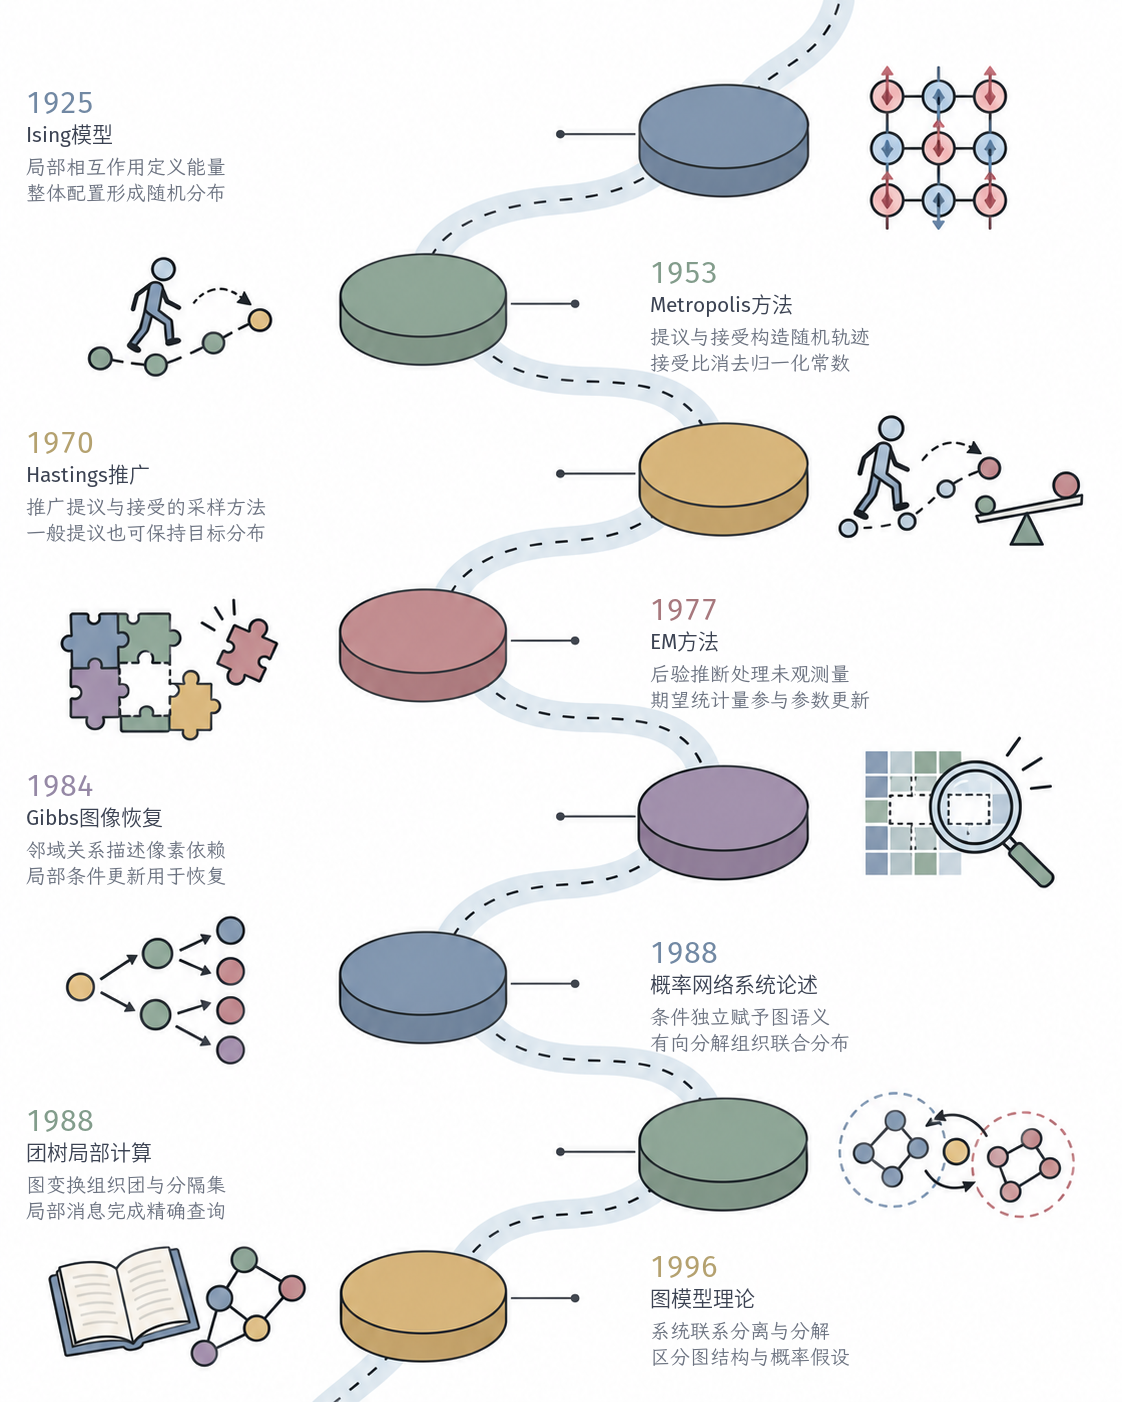
\includegraphics[width=157.406mm,height=.88\textheight,keepaspectratio]{figures/06-probabilistic-graphical-models/04-models/generated/pgm-models-history/figure.png}
\caption{概率图模型发展的代表工作（1925—1996）。沿虚线路线从上向下阅读：局部相互作用组织联合分布，随机更新估计难以直接计算的查询，潜变量学习处理缺失状态，图语义与消息计算联系独立性和推断。1988年Pearl的节点对应系统论述，而非概率网络的首次提出；节点间距不按时间比例绘制。}
  \label{fig:pgm-overview-history}
\end{figure*}
\begin{figure*}[p]
\centering
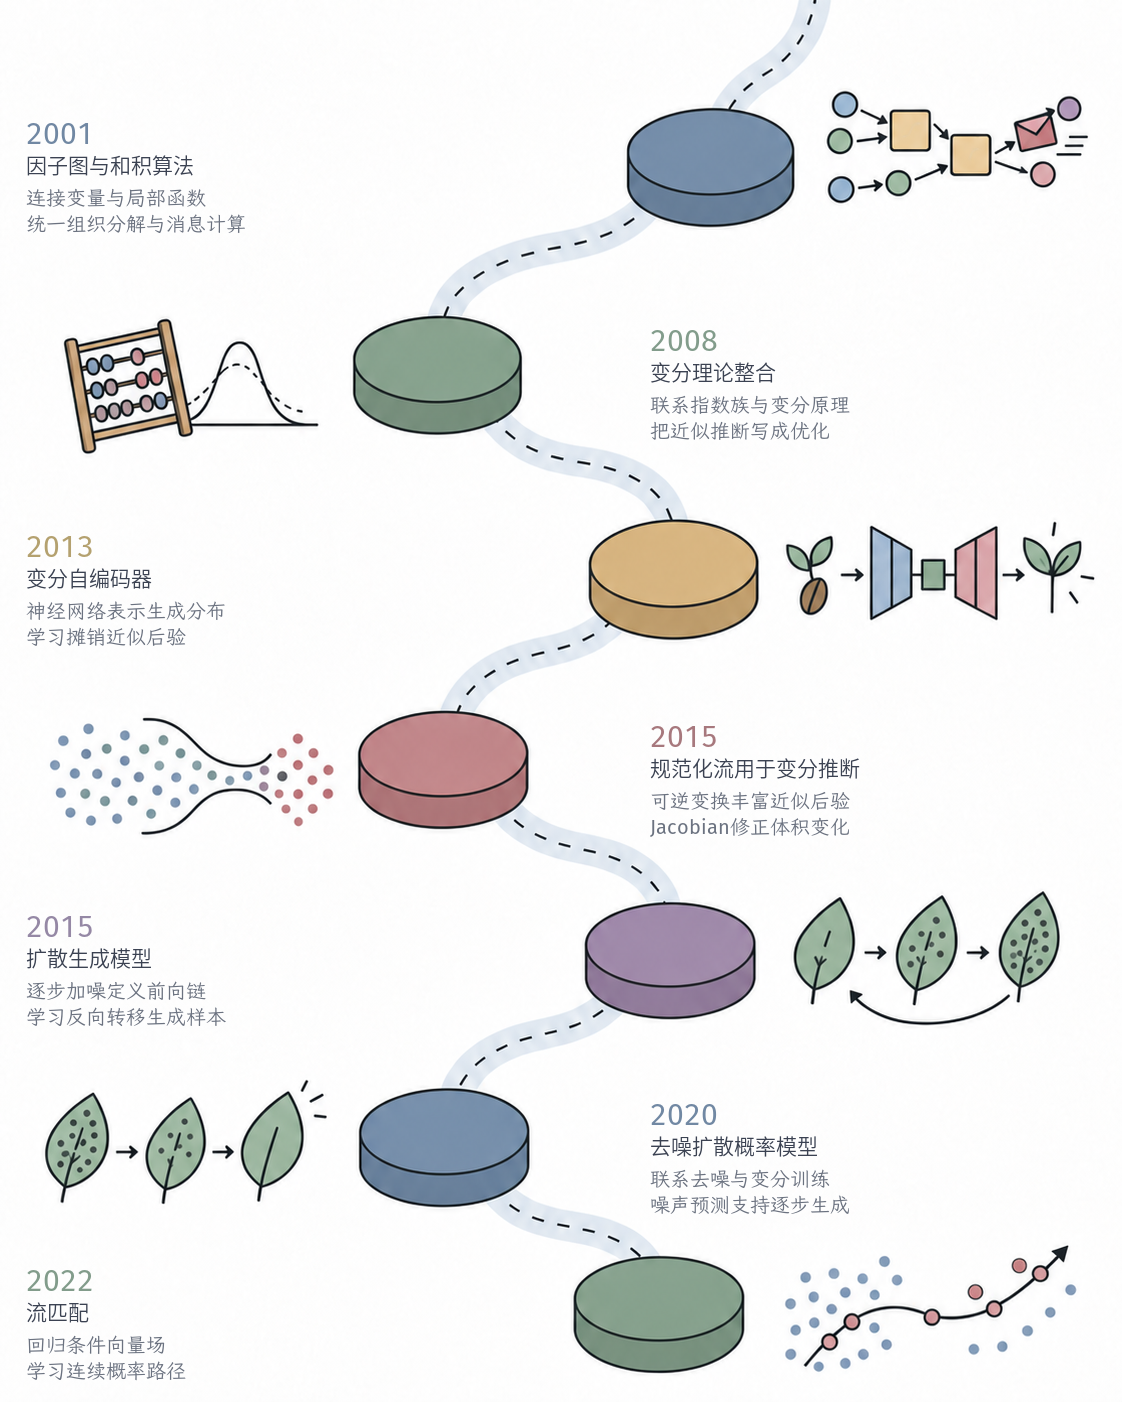
\includegraphics[width=157.406mm,height=.88\textheight,keepaspectratio]{figures/06-probabilistic-graphical-models/01-representation/generated/pgm-models-history-recent/figure.png}
\caption{概率图模型发展的代表工作（2001—2022），承接图~\ref{fig:pgm-overview-history}。因子图组织局部函数与消息，变分理论统一近似推断的优化表述，神经参数化进一步扩展后验近似和生成路径。2008年对应理论整合工作，2015年的规范化流对应流式变分推断；年份采用代表文献的首次公开或发表时间，不表示各类方法的统一起点。}
  \label{fig:pgm-overview-history-recent}
\end{figure*}

\subsection{从局部随机规律到图结构语义}

1925年的Ising模型以相邻自旋的相互作用描述整体配置，是无向局部随机模型的早期代表。每个局部项只涉及少量自旋，而归一化常数与边缘概率仍涉及整体状态的汇总。另一类问题来自数据中的未观测变量：1977年的EM方法利用当前模型推断相关统计量，再让这些统计量参与参数更新\scite{pgm-overview-ising1925,pgm-overview-dempster1977}。

归一化常数难以直接求出时，状态更新提供了另一条计算路线。1953年的Metropolis方法及1970年的Hastings推广通过提议候选状态与决定是否接受，构造随机轨迹；接受比中共同的未知归一化常数可以消去。由轨迹估计查询的效率还取决于链能否充分探索不同状态。1984年的Geman与Geman将局部相互作用定义的Gibbs分布与随机更新用于图像恢复，使局部依赖同时参与分布描述和状态计算\scite{pgm-history-metropolis1953,pgm-history-hastings1970,pgm-history-geman1984}。

1988年Pearl对概率网络的系统论述将条件独立与有向分解联系起来。同年Lauritzen与Spiegelhalter通过图变换组织局部消息，形成一般网络上的精确计算方法；1996年Lauritzen进一步系统整理图模型理论。这些工作分别为概率分解的合法性和查询的计算方式提供依据，而具体查询的开销仍由图结构决定\scite{pgm-pearl1988,pgm-overview-lauritzen1988,pgm-lauritzen1996}。

% 保留小节标题与首段，避免两页历史插画夹断近似推断的说明。
\Needspace{10\baselineskip}
\subsection{学习、近似推断与神经参数化}

大规模模型中的后验计算促使近似推断进一步发展。变分方法在可计算的分布族中优化后验近似，误差与所选分布族及优化结果有关；采样方法通过随机轨迹估计查询，有限时间内的误差与链的探索和混合行为有关。Wainwright与Jordan在2008年的综述系统联系了指数族、变分原理和图上计算\scite{pgm-wainwright2008}。

2013年以来，神经网络进入了分布及推断的参数化：VAE同时表示生成分布与近似后验，规范化流以可逆变换构造密度，扩散模型学习逆转人为加入的噪声过程。各路线提供更灵活的局部函数，同时采用不同的似然评价、后验近似和样本生成方法，因此具有不同的计算代价\scite{kingma2013,pgm-overview-rezende2015,pgm-overview-sohl2015}。

\subsection{当前研究方向}

复杂观测数据需要灵活的分布，同时也需要可承受的后验计算。一类研究设计便于计算的分解，或学习由观测直接给出后验近似的摊销方法，并评价近似误差与校准。另一类研究面向高维条件生成，考察潜变量、可逆变换、扩散和连续流分别怎样表示条件分布、怎样生成样本。流匹配通过拟合条件向量场学习连续生成路径，是其中的代表方法\scite{lipman2023flowmatching}。

对于不完整、多模态或受领域约束的数据，还需检查模型假设的依赖能否由观测识别。除生成样本的质量外，也应分别评价分布表示的准确程度、参数学习的收敛性和预测概率的可靠程度。

\section{本章小结}
\label{sec:pgm-overview-summary}

设备诊断既要判断状态，也要估计状态的概率。联合分布保留了状态间的依赖，却增加了参数和计算量。概率图模型用条件独立假设组织局部函数，并据此简化分布表示与查询计算。

有向图通过局部条件分布分解联合概率，无向图通过势函数乘积与全局归一化表示联合概率，因子图则呈现选定的局部乘积。推断在给定模型下计算概率查询，开销取决于图结构；参数学习与结构学习根据数据确定模型，潜变量使学习与推断相互联系。

下一章从有向图出发，说明条件独立与联合分解的关系。

\paragraph{扩展阅读}
Bishop的PRML第8章解释概率分解与图表示的对应；Koller与Friedman的教材进一步展开表示、推断和学习及其计算结构\scite{bishop2006,pgm-koller2009}。

\chapter{有向图模型}
\label{chap:pgm-directed}

设备报警可以为故障提供线索，传感器失灵却也可以解释同一条报警。若随后确认传感器已经失灵，故障的后验概率就可能下降。同样是增加观测，给定过热状态可以屏蔽故障与报警之间的一条联系，给定报警状态却可能让两种解释产生关联。这些变化取决于观测节点在路径上的位置，有向图为判断它们提供了规则。

本章沿用第~\ref{chap:pgm-overview}章的设备模型，先用一个固定变量顺序写出图所采用的独立性假设，再考察节点邻域及连接两组节点的路径。随后将这些关系与局部条件分布的乘积联系起来，并用离散表和连续条件分布给出可计算的模型。全局性质蕴含局部性质的图论证明随命题给出，其余跨表示证明集中在第~\ref{sec:pgm-representations-directed-proofs}节；这些结论共同说明独立性语义、联合分解和数值参数化怎样配合。

\section{有向图模型的定义}
\label{sec:pgm-directed-definition}

用四个二值随机变量表示设备状态：故障$F$、过热$H$、报警$A$和传感器失灵$S$，取值$1$表示相应状态出现。图~\ref{fig:pgm-directed-device}采用$F\to H\to A\leftarrow S$三条箭头，对应如下局部假设：过热的条件分布以故障为输入，报警的条件分布以过热和传感器状态为输入。这个结构是用于说明概率语义的人工模型，后文的数值例子也采用教学参数。

\begin{figure}[htbp]
  \centering
  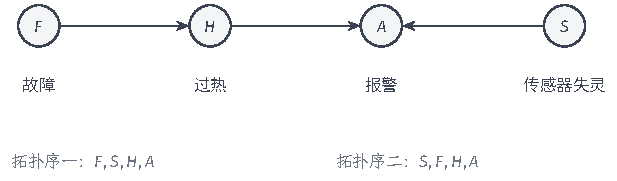
\includegraphics[width=104.482mm]{figures/06-probabilistic-graphical-models/01-representation/tikz/pgm-directed-device/figure.pdf}
  \caption{设备诊断的有向图及两个拓扑序。箭头指定局部条件分布的输入，$F$与$S$是没有父节点的根节点。下方两个序列都把父节点排在子节点之前，对应同一个图结构。}
  \label{fig:pgm-directed-device}
\end{figure}

记图为$\mathcal G=(V,E)$，其中节点对应随机变量。本部分采用有限有向无环图，并排除自环；其他结构将在使用处另行说明（相关图论约定与结论可参考\BookChapterRef{chap:graph-theory}{卷1《数学准备：计算、分析与几何》的“图的表示与计算”章}）。

局部条件分布所用的直接输入，在图中组成节点$i$的\term{父节点}（parent）集合$\operatorname{pa}(i)$；$i$直接指向的节点组成\term{子节点}（child）集合$\operatorname{ch}(i)$。将直接连接扩展为长度至少为一的有向路径，能够到达$i$的节点组成\term{祖先}（ancestor）集合$\operatorname{an}(i)$，从$i$能够到达的节点组成\term{后代}（descendant）集合$\operatorname{de}(i)$，两者都排除$i$自身。在设备图中，$\operatorname{pa}(A)=\{H,S\}$、$\operatorname{an}(A)=\{F,H,S\}$，而$\operatorname{de}(S)=\{A\}$。这些例子用变量名标记节点，一般公式则用$A\subseteq V$表示节点集合、用$\bm{X}_A$表示相应随机向量。

按顺序指定条件分布时，父节点必须先于子节点出现。有限有向无环图总能找到这样的拓扑序，而且可能有多个；图~\ref{fig:pgm-directed-device}中的$F,S,H,A$和$S,F,H,A$便是两个例子。

固定其中一个拓扑序，并将节点按该序重标记为$1,\ldots,d$。在处理节点$i$时，已经出现的节点组成\term{前驱集合}（predecessor set）$\operatorname{pre}(i)=\{1,\ldots,i-1\}$。父节点属于前驱集合，其他前驱则可能只是排在前面，例如互不相连的两个节点仍有先后次序。因此，当前顺序提供的全部条件与局部分布实际采用的父节点条件，需要分别记录。

\begin{definition}[有序Markov假设与有向图模型]
  \label{def:pgm-directed-ordered}
  给定有向图$\mathcal{G}$及一个固定拓扑序，若联合分布$p$对每个$i\in V$满足
  \begin{equation}
    X_i\perp
    \bm{X}_{\operatorname{pre}(i)\setminus\operatorname{pa}(i)}
    \mid\bm{X}_{\operatorname{pa}(i)},
    \label{eq:pgm-directed-ordered}
  \end{equation}
  则称它满足该顺序下的\term{有序Markov假设}（ordered Markov assumption）。\term{有向图模型}（directed graphical model）是有向图及其节点随机变量的联合分布，其中该联合分布满足上述假设。文献中传统上也称这类模型为\term{贝叶斯网络}（Bayesian network）；本书统一使用“有向图模型”。
\end{definition}

式~\eqref{eq:pgm-directed-ordered}将前驱中的父节点与其余节点分开：父节点给定后，其余前驱不再改变$X_i$的条件分布。这里约束的是整个分布，而均值或相关系数只描述它的部分特征。父集为空的根节点省去条件，前驱也为空时则没有需要约束的其他变量。设备顺序$F,S,H,A$中的非平凡假设写为
\[
  S\perp F,\qquad H\perp S\mid F,\qquad A\perp F\mid(H,S).
\]
这些假设当前针对选定的顺序。后面的因子分解等价关系将说明，由一个拓扑序得到的模型也满足其他合法拓扑序下的有序性质，因此所定义的模型类与具体拓扑序无关。完整证明见第~\ref{sec:pgm-representations-directed-proofs}节。

$p$表示相对于坐标参考测度乘积的联合质量或密度，条件分布等式按条件变量的分布几乎处处成立。后文用有限离散求和展示计算，密度情形在相应条件下采用积分，有向模型的结论允许联合分布取零值（条件分布及独立性的概率依据参见\BookSectionRef{sec:rv-conditional-distribution}{卷2《数学准备：概率、因果与决策》第1章“随机变量”第1.2.2.2节“条件信息下的分布关系”}与\BookSectionRef{sec:probability-moments-independence}{卷2《数学准备：概率、因果与决策》第1章“随机变量”第1.2.3节“随机变量的独立关系”}）。

有向边为局部条件分布指定可用的输入，具体参数决定该输入是否实际改变输出分布。用$F$预测$H$描述的是观测条件下的分布，主动改变$F$后的结果则需要干预语义。第~\ref{chap:pgm-structure-learning}章将讨论赋予有向结构因果解释所需的假设与识别条件。

\section{有向图的局部独立性}
\label{sec:pgm-directed-local}

给定父节点以后，哪些其他节点可以从$X_i$的条件中省去？前驱集合只能回答一个固定顺序内的问题，而图上的非后代集合可以摆脱排列。将节点自身与全部后代排除，记为
\[
  \operatorname{nd}(i)=V\setminus\bigl(\{i\}\cup\operatorname{de}(i)\bigr).
\]
父节点属于这个集合，因为父节点若同时是后代，就会与指向$i$的边组成有向环。集合排除$i$自身，随后还要把已经作为条件的父节点从待独立的变量中分出。

\begin{definition}[局部Markov性质]
  \label{def:pgm-directed-local-markov}
  分布$p$满足有向图$\mathcal{G}$的\term{局部Markov性质}（local Markov property），是指对每个节点$i$，
  \begin{equation}
    X_i\perp
    \bm{X}_{\operatorname{nd}(i)\setminus\operatorname{pa}(i)}
    \mid\bm{X}_{\operatorname{pa}(i)}.
    \label{eq:pgm-directed-local-markov}
  \end{equation}
\end{definition}

局部Markov性质用父节点屏蔽其他非后代。后代仍可能反映当前节点的状态，例如在设备模型中给定$F$以后，报警$A$还可以为过热$H$提供观测线索。因此，式~\eqref{eq:pgm-directed-local-markov}限定独立对象为非父、非后代节点。

合法拓扑序中的前驱都属于非后代，局部性质因而可以通过边缘化无须保留的独立变量，得到有序性质。相反方向涉及更多节点：在$F,S,H,A$顺序中，有序性质给出$S\perp F$，局部性质还包括排在$S$后面的$H$，即$S\perp(F,H)$。这一步需要联合分布的因子分解与祖先边缘化，证明见第~\ref{sec:pgm-representations-directed-proofs}节。

若查询要求屏蔽所有其他变量，就还要处理后代所携带的信息。能完成这种屏蔽的一组变量称为\term{Markov毯}（Markov blanket）。有向图为节点$i$提供如下标准集合：
\begin{equation}
  \begin{aligned}
    \operatorname{mb}(i)
    ={}&\operatorname{pa}(i)\cup\operatorname{ch}(i)\\
       &{}\cup\bigcup_{j\in\operatorname{ch}(i)}
           \bigl(\operatorname{pa}(j)\setminus\{i\}\bigr).
  \end{aligned}
  \label{eq:pgm-directed-blanket}
\end{equation}
该集合同时包含父节点、子节点和子节点的其他父节点，图~\ref{fig:pgm-directed-markov-blanket}分别以$P,C,U$标示。标准集合将子节点纳入条件，以处理它们对$X_i$提供的线索；给定子节点还会打开在该处碰撞的路径，于是集合同时纳入其余父节点。给定完整集合后，毯外节点$O$与$X_i$之间的路径得到屏蔽，即使$O$在原图中与毯内变量相连。

\begin{figure}[htbp]
  \centering
  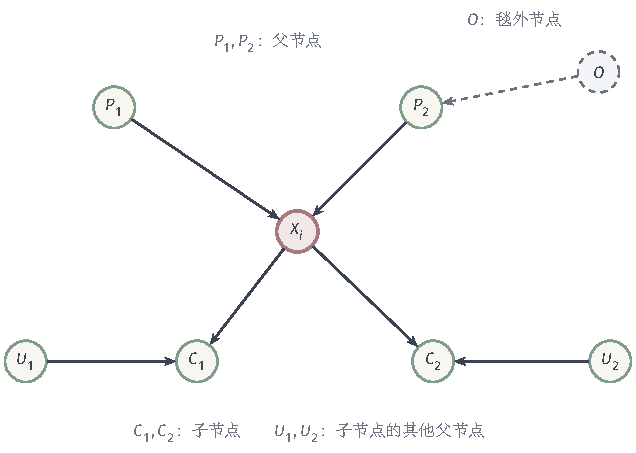
\includegraphics[width=107.685mm]{figures/06-probabilistic-graphical-models/01-representation/tikz/pgm-directed-markov-blanket/figure.pdf}
  \caption{节点$X_i$的图上Markov毯。父节点$P_1,P_2$、子节点$C_1,C_2$以及子节点的其他父节点$U_1,U_2$共同组成$\operatorname{mb}(i)$；以虚线描边的$O$位于毯外。}
  \label{fig:pgm-directed-markov-blanket}
\end{figure}

\begin{theorem}[有向图中的Markov毯]
  \label{thm:pgm-directed-markov-blanket}
  设$\mathcal{G}=(V,E)$为有限有向无环图，$p$为节点随机变量$\bm{X}=(X_i)_{i\in V}$的联合分布，且$(\mathcal{G},p)$构成有向图模型。则对每个节点$i\in V$，
  \[
    X_i\perp
    \bm{X}_{V\setminus(\{i\}\cup\operatorname{mb}(i))}
    \mid\bm{X}_{\operatorname{mb}(i)}.
  \]
\end{theorem}

在设备模型中，$\operatorname{mb}(H)=\{F,A,S\}$，其中$S$作为子节点$A$的另一个父节点进入毯。式~\eqref{eq:pgm-directed-blanket}由结构保证屏蔽关系，特定参数若产生冗余，则还可能使用更小的集合。定理~\ref{thm:pgm-directed-markov-blanket}的证明见第~\ref{sec:pgm-representations-directed-proofs}节。

\section{有向图的全局独立性}
\label{sec:pgm-directed-global}

报警状态给定后，故障与传感器失灵是否独立，涉及两个节点之间的整条路径。全局Markov性质将查询扩展为任意两组节点，由所有连接路径共同判断独立性。本节先建立路径规则，再证明全局性质能够推出局部性质和固定拓扑序下的有序性质；第~\ref{sec:pgm-directed-ci-to-factor}节将把它们与因子分解联系起来。

\subsection{两个变量之间的四种基本关系}
\label{sec:pgm-directed-motifs}

一条连接路径上的中间节点有不同的箭头形状，观测对它们的作用也不同。图~\ref{fig:pgm-directed-motifs}从直接连接、链、分叉和碰撞四种关系说明这种差别。下述三节点结论采用只有图中所画边的小图，描述结构对所有相容分布保证的独立性。在更大的图中，同样的判断用于逐条路径，最终还需检查其他连接路径；一条路径活跃时，实际依赖由具体参数决定。

\begin{figure}[htbp]
  \centering
  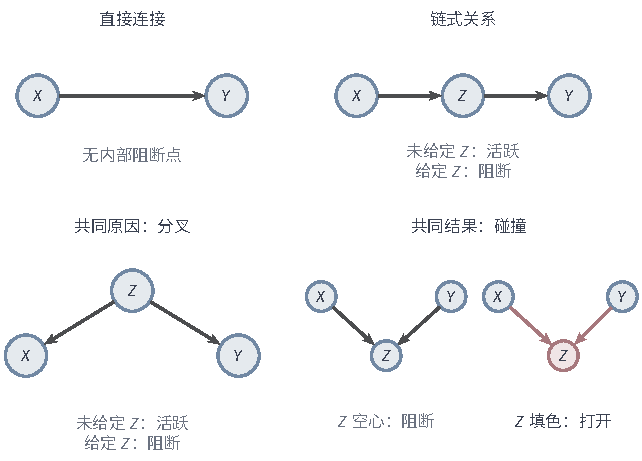
\includegraphics[width=108.793mm]{figures/06-probabilistic-graphical-models/01-representation/tikz/pgm-directed-motifs/figure.pdf}
  \caption{四种局部关系及观测中间节点后的路径变化。链和分叉在同一小图中对照两种状态；碰撞关系分为两列，空心$Z$表示未观测的阻断点，红色填充$Z$表示给定后打开的位置。活跃路径允许两端存在依赖，具体参数决定依赖是否出现。在大图中，观测碰撞点的后代也会打开该位置；直接连接没有内部阻断点。}
  \label{fig:pgm-directed-motifs}
\end{figure}

在直接连接$X\to Y$中，$X$进入$Y$的局部分布，路径中没有可用于阻断的中间节点。具体条件表若满足$p(y\mid x)=p(y)$，这个输入仍可能不改变分布，即该参数下$X\perp Y$。第~\ref{sec:pgm-directed-sound-complete}节将用数值例子说明结构允许的依赖与单个分布实际具有的依赖之间的区别。

链式关系$X\to Z\to Y$通过$Z$连接两端。采用顺序$X,Z,Y$，有序假设给出$Y\perp X\mid Z$，对应乘积$p(x,z,y)=p(x)p(z\mid x)p(y\mid z)$，一般等价证明见第~\ref{sec:pgm-representations-directed-proofs}节。给定一个满足$p(z)>0$的中间状态，条件联合分布为
\[
  p(x,y\mid z)=p(x\mid z)p(y\mid z).
\]
消去$Z$时，各个$z$下的条件分布混合在一起，两端通常仍有关联。将链反向画成$X\leftarrow Z\leftarrow Y$，给定中间节点后的独立关系相同。因此，路径判断考察内部节点的箭头形状，而非从某一端是否能沿箭头走到另一端。

分叉$X\leftarrow Z\to Y$以同一节点作为两端的条件，常用“共同原因”辨认其形状。给定$Z$时，图保证$X\perp Y\mid Z$；消去$Z$后，混合分布则可能相关。设$Z$等概率取$0$或$1$，给定$Z$后$X,Y$独立，并且两者取$1$的概率在$Z=1$时均为$0.9$，在$Z=0$时均为$0.1$。此时$p(X=1)=p(Y=1)=0.5$，而$p(X=1,Y=1)=(0.9^2+0.1^2)/2=0.41\ne0.25$。这个差值来自不同$Z$状态的混合，与每个固定$Z$下的条件独立相容。

碰撞结构$X\to Z\leftarrow Y$将两条箭头的终点放在同一个中间节点，也称“共同结果”结构。两个根节点独立，联合分解为$p(x)p(y)p(z\mid x,y)$，对$z$求和后得到$p(x,y)=p(x)p(y)$。给定$z$时，局部因子$p(z\mid x,y)$参与条件概率，可能使两端产生依赖。设$X,Y$是独立公平二值变量，$Z=1$当且仅当至少一个输入为$1$；给定$Z=1$时，$p(X=1\mid Z=1)=2/3$，再给定$Y=1$时则降为$1/2$。在这个参数设定中，确认$Y$已能解释共同结果，就降低了$X$取$1$的条件概率。这称为\term{解释消除}（explaining away），即观测共同结果后，不同解释之间产生竞争。具体依赖的方向和强弱仍由条件概率决定。

观测碰撞点的后代也可能提供关于碰撞点的信息，因此路径判据将这个位置视为打开。例如，在$X\to Z\leftarrow Y$后接$Z\to D$，若$D=Z$，观测$D$便等价于观测$Z$；若$D$是带噪声的测量，则传递的信息量取决于噪声水平。碰撞点及全部后代均未给定时，该位置才由图保证阻断。这里的“共同原因”和“共同结果”描述箭头形状，其因果解释需要另行建立。

\begin{figure}[htbp]
  \centering
  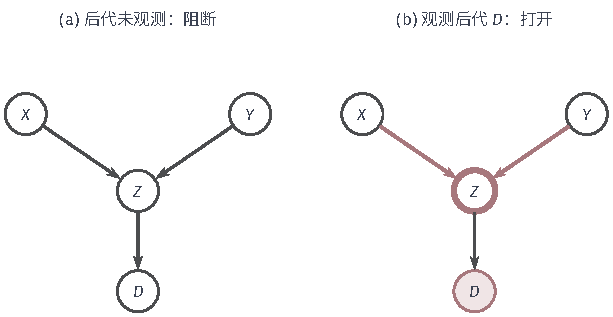
\includegraphics[width=103.720mm]{figures/06-probabilistic-graphical-models/01-representation/tikz/pgm-directed-collider-descendant/figure.pdf}
  \caption{后代观测对碰撞位置的作用。左图中$Z$及其后代均未给定，路径$X\to Z\leftarrow Y$被阻断；右图将后代$D$填色为观测，空心双圈$Z$标出已打开的碰撞位置，红色路径满足$Z\in\operatorname{an}^{+}(S)$。图上打开的路径允许依赖出现，依赖强度由分布决定。}
  \label{fig:pgm-directed-collider-descendant}
\end{figure}

\subsection{d-分离的定义}
\label{sec:pgm-directed-d-separation}

两组节点在给定条件后仍可能通过多条路径联系，因而分离查询需要汇总全部路径的判断。路径上的非碰撞点被给定时阻断路径，碰撞点自身或后代被给定时则打开该位置。对两两不交的$A,B,S\subseteq V$，若$A,B$之间不存在活跃路径，就记$A\perp_{\mathcal G}B\mid S$。这个记号先描述图上的分离，随后将说明它与概率独立的关系。为表达碰撞点的观测条件，后文用$\operatorname{an}^{+}(T)$表示包含$T$自身的祖先闭包。

设备路径中的$A$是碰撞点，$H$是非碰撞点，图~\ref{fig:pgm-directed-active-path}对照了给定它们后的变化。只给定$A$时路径活跃，再给定$H$时路径在$H$处阻断。整条路径活跃需要每个内部位置都满足条件，因此一个位置的打开无法消除另一位置的阻断。

\begin{figure}[htbp]
  \centering
  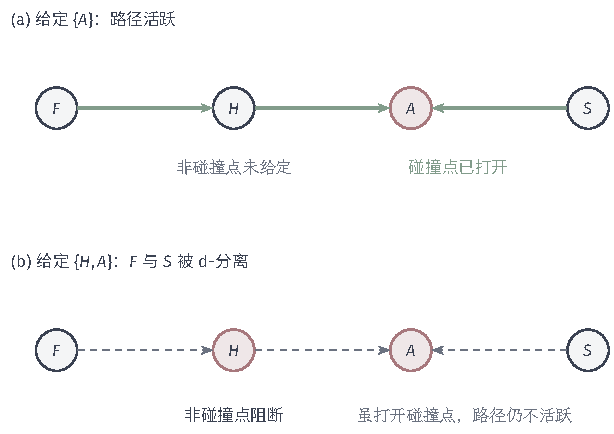
\includegraphics[width=103.904mm]{figures/06-probabilistic-graphical-models/01-representation/tikz/pgm-directed-active-path/figure.pdf}
  \caption{设备路径的活跃状态与d-分离。上图给定碰撞点$A$后，$F\to H\to A\leftarrow S$活跃；下图再给定非碰撞点$H$后，唯一的连接路径被阻断，得到$F\perp_{\mathcal{G}}S\mid(H,A)$。红色节点为给定变量，绿色实线为活跃路径，灰色虚线为阻断路径。}
  \label{fig:pgm-directed-active-path}
\end{figure}

图上的$A\perp_{\mathcal G}B\mid S$与分布中的$\bm{X}_A\perp\bm{X}_B\mid\bm{X}_S$分别描述路径和概率关系。\term{全局Markov性质}（global Markov property）把两者接起来：对每个两两不交的查询$(A,B,S)$，图中的d-分离蕴含相应的分布独立。第~\ref{sec:pgm-directed-sound-complete}节将说明相容分布为何满足这个蕴含。

\begin{lemma}[全局Markov性质蕴含局部Markov性质]
  \label{lem:pgm-representations-global-to-local}
  设$\mathcal{G}=(V,E)$为有限有向无环图，$p$为节点随机变量$\bm{X}=(X_i)_{i\in V}$的联合分布。若$p$满足$\mathcal{G}$的全局Markov性质，则$p$也满足该图的局部Markov性质，并进一步满足任一固定拓扑序下的有序Markov性质。
\end{lemma}

\begin{proof}[引理~\ref{lem:pgm-representations-global-to-local}的证明]
固定节点$i$，逐一考察它到非父、非后代节点的路径。路径若在$i$处经过一条入边，邻接的父节点就是内部非碰撞点，给定$\operatorname{pa}(i)$即可在此阻断。路径若先沿$i$的出边前进，则到达非后代之前必须改变沿箭头前进的方向；第一次转折产生一个碰撞点，并且该点是$i$的后代。这个碰撞点及其后代均在父集之外，否则有向路径与入边会构成环，因而给定父集后该碰撞点保持阻断。两类路径都被阻断，得到
\[
  i\perp_{\mathcal G}
  \operatorname{nd}(i)\setminus\operatorname{pa}(i)
  \mid\operatorname{pa}(i).
\]
将该图分离代入全局Markov性质，便得到局部Markov性质。合法拓扑序的前驱包含于非后代集合，从局部独立陈述中边缘化其他非后代，又得到该拓扑序下的有序Markov性质。
\end{proof}

在设备图中，$F,S$只有$F\to H\to A\leftarrow S$这一条连接路径。无观测时，碰撞点$A$阻断它，得到$F\perp S$；给定报警$A$后，碰撞位置打开而$H$保持未观测，路径转为活跃；再给定$H$后又得到$F\perp S\mid(H,A)$。如果增加$A\to D$，观测$D$同样会打开$A$，因为它提供了碰撞点后代的证据。

条件集合$S$记录被给定的变量，而具体取值另行指定。d-分离所对应的条件独立对条件变量分布几乎处处成立，涵盖整项条件关系。某些参数还可能只在特定条件取值下产生独立，这类上下文性质来自具体分布，须与图上的分离查询分别处理。

\subsection{d-分离的可靠性与特定场景下的完备性}
\label{sec:pgm-directed-sound-complete}

同一张图可以配上不同的条件概率表，路径判据因而需要在分布类上解释。分离查询应对所有相容分布成立，而未分离查询需要考察是否存在实际依赖的相容分布。记$\mathcal{M}(\mathcal{G})$为定义~\ref{def:pgm-directed-ordered}所给模型的分布类；第~\ref{sec:pgm-directed-factorization}节将说明它与按$\mathcal{G}$分解的分布类等价，证明见第~\ref{sec:pgm-representations-directed-proofs}节。

\begin{theorem}[d-分离的可靠性]
  \label{thm:pgm-directed-soundness}
  设$\mathcal{G}=(V,E)$为有限有向无环图，$A,B,S\subseteq V$两两不交且$A,B$非空。对每个$p\in\mathcal{M}(\mathcal{G})$，
  \begin{equation}
    A\perp_{\mathcal{G}}B\mid S
    \quad\Longrightarrow\quad
    \bm{X}_A\perp_p\bm{X}_B\mid\bm{X}_S.
    \label{eq:pgm-directed-soundness}
  \end{equation}
\end{theorem}

\begin{example}[未分离但独立的固定分布]
  \label{ex:pgm-directed-unseparated-independent}
  在只有一条边$X\to Y$的图中，令$X,Y\in\{0,1\}$，并设$p(X=0)=p(X=1)=1/2$。对每个$x\in\{0,1\}$，都取$p(Y=1\mid X=x)=1/3$和$p(Y=0\mid X=x)=2/3$。图上两个节点直接相邻，空集无法将它们d-分离；条件表的两行却相同，边缘化$X$得到$p(Y=1)=1/3$和$p(Y=0)=2/3$。由此对所有$x,y\in\{0,1\}$有
  \[
    p(X=x,Y=y)
    =
    p(X=x)p(Y=y)
    =
    \begin{cases}
      1/6,&y=1,\\
      1/3,&y=0.
    \end{cases}
  \]
  这个乘积等式给出该固定分布中的$X\perp Y$，说明相邻节点在某些参数下也能独立。
\end{example}

示例~\ref{ex:pgm-directed-unseparated-independent}区分了已选定的分布与可选的分布类。该分布中的依赖可以消失，而在充分丰富的分布类中，每项未分离查询仍有至少一个相容分布表现出依赖。后一种存在性结论称为\term{模型类完备性}，以下分别在严格正有限离散模型类与非退化线性高斯模型类中陈述。

\term{严格正有限离散模型}中，每个变量有有限个状态，每个完整配置的联合概率均大于$0$。固定状态空间$\mathcal{X}_i$并要求$|\mathcal{X}_i|\geq2$，将其中严格为正且按$\mathcal{G}$分解的质量函数记为$\mathcal{M}_{\mathrm{disc}}^{+}(\mathcal{G})$。\term{非退化线性高斯模型}则以父节点的线性函数加独立高斯噪声表示当前节点；正噪声方差保证联合分布具有完整维度。将所有由下式生成的分布记为$\mathcal{M}_{\mathrm{LG}}(\mathcal{G})$：
\[
  X_i=a_i+\sum_{j\in\operatorname{pa}(i)}b_{i,j}X_j+\varepsilon_i
\]
其中边系数$b_{i,j}$可取任意实数，噪声$\varepsilon_i$相互独立，满足$\varepsilon_i\sim\mathcal{N}(0,\sigma_i^2)$及$\sigma_i^2>0$。

\begin{theorem}[d-分离在特定模型类中的完备性]
  \label{thm:pgm-directed-completeness}
  设$\mathcal{G}=(V,E)$为有限有向无环图，$A,B,S\subseteq V$两两不交且$A,B$非空。若
  \[
    A\not\perp_{\mathcal{G}}B\mid S,
  \]
  则分别存在$p_{\mathrm{disc}}\in\mathcal{M}_{\mathrm{disc}}^{+}(\mathcal{G})$与$p_{\mathrm{LG}}\in\mathcal{M}_{\mathrm{LG}}(\mathcal{G})$，使
  \begin{equation}
    \bm{X}_A\not\perp_{p_{\mathrm{disc}}}\bm{X}_B\mid\bm{X}_S,
    \qquad
    \bm{X}_A\not\perp_{p_{\mathrm{LG}}}\bm{X}_B\mid\bm{X}_S.
    \label{eq:pgm-directed-completeness}
  \end{equation}
\end{theorem}

可靠性覆盖每个相容分布，模型类完备性则为每项未分离查询提供一个不独立的见证分布，不同查询还可以使用不同见证。两种结论采用不同量词，因此完备性与前面的固定分布反例相容。两个定理的证明见第~\ref{sec:pgm-representations-directed-proofs}节。

从观测到的条件独立反推图结构时，上例的相同行会造成歧义：独立可能来自缺边，也可能来自参数。

对于$p\in\mathcal{M}(\mathcal{G})$，模型的Markov性已经使图分离推出概率独立。忠实性进一步要求，每项分布独立都能由图分离解释（参见\BookDefinitionRef{def:causal-faithfulness}{卷2《数学准备：概率、因果与决策》第3章“因果响应”第3.6.1.1节“观测资料下的关系识别”}）。两个方向共同成立时，图与分布的独立关系集合相同。

确定性关系、强制参数共享和参数抵消都可能产生额外独立性。有向分解允许这些参数，而忠实性对分布施加进一步限制。结构学习在依据独立性删边时，需要说明所采用的忠实性假设及其适用依据。

\subsection{d-分离的检测}
\label{sec:pgm-directed-d-separation-testing}

路径判据可直接用于小图，但大图可能包含很多重复经过同一节点的路径。检测算法可以合并这些路径的到达状态，也可以将当前查询转为无向图的连通性检查。下面分别说明这两种计算方式如何利用结构。

\begingroup
% tufte-book禁用subsubsection；本节局部沿用其支持的第三级paragraph样式。
\let\subsubsection\paragraph

\subsubsection{Bayes--ball算法}
\label{sec:pgm-directed-bayes-ball}

设备图对$F,S$的查询只有一条连接路径，可以按内部节点的角色逐项检查，结果列于表~\ref{tab:pgm-directed-path-tests}。给定$H$使路径阻断，给定$A$则使碰撞位置打开，同时给定两者时仍由$H$阻断。观测增加后的变化由路径位置决定，而非条件集合大小决定。

\begin{table}[htbp]
  \centering
  \begin{tabularx}{\linewidth}{@{}lXX@{}}
    \toprule
    给定节点 & 路径上的检查 & 图的结论 \\
    \midrule
    $\varnothing$ & 碰撞点$A$未打开 & $F$与$S$分离 \\
    $\{H\}$ & 非碰撞点$H$阻断 & $F$与$S$分离 \\
    $\{A\}$ & $A$打开，$H$未阻断 & $F$与$S$连接 \\
    $\{H,A\}$ & $A$虽打开，$H$仍阻断 & $F$与$S$分离 \\
    \bottomrule
  \end{tabularx}
  \caption{设备路径$F\to H\to A\leftarrow S$在不同条件集合下的检查结果。“分离”给出图保证的独立性，“连接”表示结构允许依赖出现，实际依赖仍取决于参数。}
  \label{tab:pgm-directed-path-tests}
\end{table}
\FloatBarrier

为避免枚举可能呈指数增长的路径数，\term{Bayes--ball算法}（Bayes-ball algorithm）将搜索状态设为当前节点及到达方向，相同状态只处理一次。算法~\ref{alg:pgm-directed-bayes-ball}采用专门检测d-分离的版本，按照图结构传播状态；利用已知确定性关系作额外剪枝或计算后验属于其他任务。状态$(i,\uparrow)$表示从$i$的子节点一侧到达，$(i,\downarrow)$表示从父节点一侧到达。

\begin{algorithm}[Bayes--ball的d-分离检测]
  \label{alg:pgm-directed-bayes-ball}
  \begin{algorithmic}[1]
    \Require 有向图$\mathcal{G}=(V,E)$，两两不交的$A,B,S\subseteq V$，且$A,B$非空
    \Ensure “d-连接”或“d-分离”
    \State $R\gets\operatorname{an}^{+}(S)$
    \State 队列$Q\gets\{(a,\uparrow):a\in A\}$
    \State 已处理状态集$M\gets\varnothing$
    \While{$Q$非空}
      \State 从$Q$取出$(i,\delta)$
      \If{$(i,\delta)\in M$}
        \State 转到下一轮循环
      \EndIf
      \State $M\gets M\cup\{(i,\delta)\}$
      \If{$i\in B$}
        \State \Return d-连接
      \EndIf
      \If{$\delta=\uparrow$且$i\notin S$}
        \State 向$Q$加入$\{(j,\uparrow):j\in\operatorname{pa}(i)\}$
        \State 向$Q$加入$\{(j,\downarrow):j\in\operatorname{ch}(i)\}$
      \ElsIf{$\delta=\downarrow$}
        \If{$i\notin S$}
          \State 向$Q$加入$\{(j,\downarrow):j\in\operatorname{ch}(i)\}$
        \EndIf
        \If{$i\in R$}
          \State 向$Q$加入$\{(j,\uparrow):j\in\operatorname{pa}(i)\}$
        \EndIf
      \EndIf
    \EndWhile
    \State \Return d-分离
  \end{algorithmic}
\end{algorithm}

起点以子侧状态入队，使搜索能够沿入边和出边向外传播。从子侧到达$i$时，$i$在接续路径中是非碰撞点，满足$i\notin S$便可向父节点或子节点继续传播。从父侧到达$i$后，向子节点传播仍需$i\notin S$，向另一个父节点传播则在$i$处形成碰撞，需满足$i\in R$，即$i$自身或后代被观测。后两项判断独立执行，因此两种传播都可能发生；它们分别落实了路径定义中的非碰撞与碰撞条件。

在查询$F\perp S\mid A$中，$R=\{F,H,A,S\}$。搜索依次到达$F,H$，再从父侧到达$A$；因为$A$属于$R$，搜索转向其父节点$S$，发现一条活跃路径。将条件集合改为$\{H,A\}$后，观测节点$H$阻止向子节点$A$传播，搜索无法到达$S$。记录到达方向保留了这两类传播的区别，只有节点访问标记则会把不同搜索状态合并。

集合$R$通过从$S$逆向遍历祖先取得。随后每个节点至多处理两个到达状态，每条边由这些状态扫描常数次，因此时间和存储量均为$O(|V|+|E|)$\scite{pgm-directed-shachter1998}。

\subsubsection{祖先道德图检测}
\label{sec:pgm-directed-ancestral-moral-test}
\label{sec:pgm-directed-undirected-test}

同一个查询还可以通过\term{祖先道德图检测}转为连通性问题。保留$A\cup B\cup S$及其全部祖先，在这个子图中将共同子节点的父节点两两相连，再去掉箭头方向；删除条件节点$S$后，检查$A$与$B$是否连通。选取祖先子图这一步使转换依赖当前查询，区别于单纯去掉原图的方向。第~\ref{sec:pgm-representations-ancestral-moralization}节将正式定义该转换，证明它与d-分离等价，并分析代价。祖先道德图检测与Bayes--ball均输出结构分离结果，后验数值仍需概率运算。

\endgroup

\section{有向图中的因子分解}
\label{sec:pgm-directed-factorization}

\subsection{因子分解的定义}
\label{sec:pgm-directed-factor-definition}

设备模型的独立性假设确定了每个节点要保留的父节点条件，存储联合概率时则需要把这些局部分布组合起来。\term{有向因子分解}（directed factorization）将每个节点给定父节点的条件分布相乘。每一项都按当前节点归一化，使其在固定父配置下成为合法的条件分布。

组合局部函数还需要一个统一的联合积分空间。下文采用$\sigma$有限基准测度，即状态空间可由可数个有限测度的集合覆盖；有限或可数状态的计数测度以及实数轴上的Lebesgue测度都符合这一条件。单坐标的可测事件由$\mathcal A_i$记录，它们的笛卡尔积生成乘积$\sigma$代数$\bigotimes_i\mathcal A_i$，作为联合可测事件集合。分解式中的“$\mu$几乎处处”针对乘积基准测度的零测集，改变这些位置的密度不会改变积分所得概率；前面的条件独立等式则以条件变量的边缘分布为参照，两处采用的测度不同。

\begin{definition}[按有向图分解]
  \label{def:pgm-directed-factorization}
  给定有限有向图$\mathcal{G}=(V,E)$，其中$V=\{1,\ldots,d\}$。节点$i$取值于可测空间$(\mathcal{X}_i,\mathcal{A}_i)$，其上指定$\sigma$有限基准测度$\mu_i$；记$(\mathcal{X},\mathcal{A})=(\prod_{i\in V}\mathcal{X}_i,\bigotimes_{i\in V}\mathcal{A}_i)$及$\mu=\bigotimes_{i\in V}\mu_i$。设联合分布$p$对$\mu$绝对连续，并仍用$p(\bm{x})$表示其可测密度。对每个节点$i$，选定局部条件质量函数或条件密度版本
  \[
    q_i:
    \mathcal{X}_i\times
    \prod_{j\in\operatorname{pa}(i)}\mathcal{X}_j
    \longrightarrow[0,\infty).
  \]
  要求$q_i$关于相应乘积$\sigma$代数可测，并对每个父节点配置$\bm{x}_{\operatorname{pa}(i)}$满足
  \[
    \int_{\mathcal{X}_i}
    q_i(x_i\mid\bm{x}_{\operatorname{pa}(i)})\,\mathrm{d}\mu_i(x_i)=1.
  \]
  若
  \begin{equation}
    p(\bm{x})=\prod_{i=1}^{d}
      q_i(x_i\mid\bm{x}_{\operatorname{pa}(i)})
      \qquad\text{$\mu$几乎处处},
    \label{eq:pgm-directed-factorization}
  \end{equation}
  就称$p$按有向图$\mathcal{G}$分解。父集为空时，对应因子$q_i(x_i)$是归一化的边缘质量函数或密度。有限离散变量情形取$\mathcal{A}_i=2^{\mathcal{X}_i}$和计数测度$\mu_i$，上述积分即求和，$p$与$q_i$均为概率质量函数，式~\eqref{eq:pgm-directed-factorization}对每个完整配置$\bm{x}$逐点成立；零质量父配置采用本章约定的归一化条件质量函数版本。连续变量情形中，$q_i$是相对于已指定$\mu_i$的条件密度版本，式~\eqref{eq:pgm-directed-factorization}相对于已定义的乘积测度$\mu$几乎处处成立；在零测集上改变密度版本不改变所表示的分布。
\end{definition}

上述定义判断给定的联合分布$p$是否具有所需分解。实际构造模型时，常常先指定各节点的局部条件函数，再将它们相乘，此时需要验证乘积已经归一化。下面的引理给出这项保证，并进一步说明：若保留的节点集合包含自身的全部祖先，消去其余节点后，边缘密度就是保留节点的局部函数乘积。状态空间、基准测度、可测性和局部归一化的条件在引理中一并列出。

\begin{lemma}[局部归一化与祖先边缘化]
  \label{lem:pgm-directed-normalization}
  设$\mathcal{G}=(V,E)$为有限有向无环图，$V=\{1,\ldots,d\}$。节点$i$取值于可测空间$(\mathcal{X}_i,\mathcal{A}_i)$，其上给定$\sigma$有限基准测度$\mu_i$；有限离散变量取计数测度。对每个节点$i$，设局部函数
  \[
    q_i:
    \mathcal{X}_i\times
    \prod_{j\in\operatorname{pa}(i)}\mathcal{X}_j
    \longrightarrow[0,\infty)
  \]
  关于相应乘积$\sigma$代数可测，并对每个父节点配置满足
  \[
    \int_{\mathcal{X}_i}
    q_i(x_i\mid\bm{x}_{\operatorname{pa}(i)})\,\mathrm{d}\mu_i(x_i)=1.
  \]
  相对于乘积测度$\mu=\bigotimes_{i\in V}\mu_i$定义
  \[
    q(\bm{x})=\prod_{i\in V}
    q_i(x_i\mid\bm{x}_{\operatorname{pa}(i)}).
  \]
  则$q$归一化，因而是某个联合分布$p$的密度。更一般地，若$W\subseteq V$包含其中每个节点的全部祖先，则$p$关于$\mu_W=\bigotimes_{i\in W}\mu_i$的边缘密度满足
  \begin{equation}
    p(\bm{x}_W)=
    \prod_{i\in W}q_i(x_i\mid\bm{x}_{\operatorname{pa}(i)}).
    \label{eq:pgm-directed-ancestral-marginal}
  \end{equation}
  该等式对$\mu_W$几乎处处成立；有限离散情形中则对每个$\bm{x}_W$逐点成立。
\end{lemma}

无环结构使归一化能够从末端节点逐项消元，引理~\ref{lem:pgm-directed-normalization}的完整证明见第~\ref{sec:pgm-representations-directed-proofs}节。有向环的反例说明这个条件的作用：在二值环$X\to Y\to X$上取$q_X(x\mid y)=\mathbf{1}\{x=y\}$、$q_Y(y\mid x)=\mathbf{1}\{y=x\}$，两个条件表各自归一化，乘积在$(0,0)$和$(1,1)$上却都为$1$，总和为$2$。环使末端消元无法进行，所以局部归一化在这里没有给出联合归一化。

设备图中的四个局部表对应如下联合分解：
\begin{equation}
  p(f,h,a,s)=p(f)p(s)p(h\mid f)p(a\mid h,s).
  \label{eq:pgm-directed-device-factor}
\end{equation}
用第~\ref{sec:pgm-directed-discrete}节列出的教学参数，可以逐项求出配置$F=1,H=1,A=1,S=0$的联合概率：
\begin{equation}
  \begin{aligned}
    &p(F=1,H=1,A=1,S=0)\\
    &\quad=p(F=1)p(S=0)p(H=1\mid F=1)
      p(A=1\mid H=1,S=0)\\
    &\quad=0.1\times0.95\times0.8\times0.9
      =0.0684.
  \end{aligned}
  \label{eq:pgm-directed-device-configuration}
\end{equation}
计算结果$0.0684$来自四个局部表项的乘积，因而完整联合表中的这一项可以在使用时求得。消去变量时也能利用分解，例如求$F,H$的边缘分布，可以先汇总报警状态，再汇总传感器状态：
\[
  \begin{aligned}
    p(f,h)
    &=p(f)p(h\mid f)
      \sum_s p(s)\sum_a p(a\mid h,s)\\
    &=p(f)p(h\mid f).
  \end{aligned}
\]
内层报警概率的和为$1$，随后传感器概率的和也为$1$，因此只剩$F,H$的两个因子。有限求和的顺序可以交换，结果保持相同，中间函数的作用域与大小却可能改变。第~\ref{chap:pgm-elimination}章将据此分析消元顺序的计算代价。

\subsection{从因子分解到条件独立性}
\label{sec:pgm-directed-factor-to-ci}

在完整联合乘积中，$x_i$既出现在节点$i$自己的因子，也出现在子节点的因子中。要得到节点$i$给定非后代的条件分布，需要先边缘化后代，利用祖先边缘分解消去这些子节点因子。这样才可从剩余局部项读出所需独立性。

\begin{theorem}[分解蕴含局部与有序Markov性质]
  \label{thm:pgm-directed-factor-local}
  设$\mathcal{G}=(V,E)$为有限有向无环图，$p$为节点随机变量$\bm{X}=(X_i)_{i\in V}$的联合分布。若$p$按$\mathcal{G}$分解，则$p$满足该图的局部Markov性质，并满足该图任一固定拓扑序下的有序Markov性质。
\end{theorem}

定理~\ref{thm:pgm-directed-factor-local}将因子分解连接到局部和有序Markov性质，定理~\ref{thm:pgm-directed-soundness}的可靠性结论再将它连接到全局Markov性质。相应证明集中在第~\ref{sec:pgm-representations-directed-proofs}节。

\subsection{从条件独立性到因子分解}
\label{sec:pgm-directed-ci-to-factor}

反向构造从定义中的固定拓扑序开始。链式法则先为每个节点保留全部前驱条件，有序Markov假设再将其缩为父节点条件，从而得到所需乘积。

\begin{theorem}[有序假设导出有向分解]
  \label{thm:pgm-directed-ordered-factor}
  设$\mathcal{G}=(V,E)$为有限有向无环图，$p$为节点随机变量$\bm{X}=(X_i)_{i\in V}$的联合分布，并采用定义~\ref{def:pgm-directed-factorization}中的有限离散质量函数或连续密度设定。若$p$满足$\mathcal{G}$的某一个固定拓扑序下的有序Markov假设，则$p$按$\mathcal{G}$分解。
\end{theorem}

定理~\ref{thm:pgm-directed-factor-local}和定理~\ref{thm:pgm-directed-ordered-factor}给出有序性质与分解之间的两个方向，局部性质又蕴含有序性质。加上d-分离可靠性及全局到局部的蕴含，四种表述连成如下等价关系：
\begin{equation}
  \begin{aligned}
    \text{固定拓扑序的有序性质}
      &\Longleftrightarrow \text{按有向图分解}\\
      &\Longleftrightarrow \text{局部Markov性质}\\
      &\Longleftrightarrow \text{全局Markov性质}.
  \end{aligned}
  \label{eq:pgm-directed-equivalence}
\end{equation}
这个等价关系说明，一个拓扑序下的有序假设已经确定模型类：先由该序得到分解，再由分解得到任一合法拓扑序下的有序性质。上述有向结论允许零概率配置，与后文无向分解定理的严格正性要求有所区别。全局到局部的方向已由引理~\ref{lem:pgm-representations-global-to-local}证明，其余方向见第~\ref{sec:pgm-representations-directed-proofs}节。

式~\eqref{eq:pgm-directed-equivalence}检验一个给定分布的模型归属。定理~\ref{thm:pgm-directed-completeness}则处理另一种量词：对每个未分离查询，在指定模型类中构造至少一个不独立的见证分布。这项构造的证明也见第~\ref{sec:pgm-representations-directed-proofs}节。

\section{局部参数化}
\label{sec:pgm-directed-local-parameterization}

设备诊断的结构已确定报警使用$H,S$作条件，接下来还要给出每种条件下的报警概率。局部参数化负责记录这些数值，并支持估计和采样。本节分别讨论离散表与连续条件分布，它们提供不同的局部函数形式，共同遵循前面的有向分解。

\subsection{离散变量}
\label{sec:pgm-directed-discrete}

对于离散节点，父配置固定后，只需记录各个子状态的概率。若$X_i$有$r_i$个状态、父节点有$c_i=\prod_{j\in\operatorname{pa}(i)}r_j$种配置，\term{条件概率表}（conditional probability table, CPT）为每个父配置设置一个长度$r_i$的向量。各行非负且和为$1$，每行有$r_i-1$个自由参数，所以无额外约束的表共有$c_i(r_i-1)$个自由参数。对所有节点求和，得到网络的参数自由度：
\begin{equation}
  m=\sum_{i=1}^{d}(r_i-1)
       \prod_{j\in\operatorname{pa}(i)}r_j.
  \label{eq:pgm-directed-cpt-size}
\end{equation}
若每个变量最多有$r$个状态、每个节点最多有$k$个父节点，完整条件表的存储空间为$O(dr^{k+1})$。因此，父集大小决定一张局部表包含多少行，是控制离散表示规模的关键条件。

设备模型中的二值根节点各需一个参数，$H$的两个父配置和$A$的四个父配置分别需要两个、四个参数，总计$1+1+2+4=8$个。相同四变量的无约束联合表则需要$2^4-1=15$个参数。以下教学设定给出根节点与过热节点的局部数值：
\[
  \begin{aligned}
    p(F=1)&=0.1,& p(S=1)&=0.05,\\
    p(H=1\mid F=1)&=0.8,&
    p(H=1\mid F=0)&=0.1.
  \end{aligned}
\]
报警节点的四行列在表~\ref{tab:pgm-directed-alarm-cpt}中，每行取$0$的概率为取$1$概率的余数。

\begin{table}[htbp]
  \centering
  \begin{tabular}{@{}ccrr@{}}
    \toprule
    $h$ & $s$ & $p(A=1\mid h,s)$ & $p(A=0\mid h,s)$ \\
    \midrule
    $0$ & $0$ & $0.01$ & $0.99$ \\
    $1$ & $0$ & $0.90$ & $0.10$ \\
    $0$ & $1$ & $0.70$ & $0.30$ \\
    $1$ & $1$ & $0.99$ & $0.01$ \\
    \bottomrule
  \end{tabular}
  \caption{教学模型的报警条件概率表。每个固定$(h,s)$对应一行二值概率分布，两项之和为$1$；数值为人工设定。}
  \label{tab:pgm-directed-alarm-cpt}
\end{table}

用这些局部数值，可以计算章首所问的观测变化。先消去故障和传感器状态，得到过热与报警的概率：
\[
  \begin{aligned}
    p(H=1)&=0.1\times0.8+0.9\times0.1=0.17,\\
    p(A=1\mid H=1)&=0.95\times0.9+0.05\times0.99=0.9045,\\
    p(A=1\mid H=0)&=0.95\times0.01+0.05\times0.7=0.0445,\\
    p(A=1)&=0.17\times0.9045+0.83\times0.0445=0.1907.
  \end{aligned}
\]
报警后过热概率为$0.153765/0.1907\approx0.8063$。再给定传感器失灵，另一种解释进入条件，过热后验变为
\[
  p(H=1\mid A=1,S=1)
    =\frac{0.17\times0.99}
      {0.17\times0.99+0.83\times0.7}
    \approx0.2246.
\]
将仍未知的过热状态边缘化，同样可以比较故障在两组证据下的后验：
\[
  \begin{aligned}
    p(F=1\mid A=1)&=\frac{0.07325}{0.1907}\approx0.3841,\\
    p(F=1\mid A=1,S=1)&=\frac{0.0932}{0.7493}\approx0.1244.
  \end{aligned}
\]
在这组参数中，传感器失灵解释了一部分报警，使故障后验从约$0.3841$降到约$0.1244$。这是解释消除的一个具体数值结果，路径判据则说明给定报警为何允许两种解释发生关联。

完整观测数据还能直接估计这些表。设有$n$个独立同分布样本$\{\bm{x}_{\ell}\}_{\ell=1}^{n}$，所有节点均已观测，图固定且局部表参数没有共享约束。将父配置为$a$且$X_i=k$的样本数记为$N_{i,a,k}$，行计数记为$N_{i,a}=\sum_kN_{i,a,k}$，该项条件概率记为$\theta_{i,a,k}$。对数似然于是按节点和父配置分开，逐行最大化给出
\[
  \begin{aligned}
    \ell(\bm{\theta})
       &=\sum_i\sum_a\sum_kN_{i,a,k}\log\theta_{i,a,k},\\
    \widehat{\theta}_{i,a,k}&=\frac{N_{i,a,k}}{N_{i,a}}.
  \end{aligned}
\]
每行概率和为$1$的约束下，计数比例给出$N_{i,a}>0$时的极大值。$N_{i,a}=0$的行没有样本支持，数据无法确定该行的参数。加入正伪计数$\alpha_{i,a,k}$，可得到平滑估计$(N_{i,a,k}+\alpha_{i,a,k})/(N_{i,a}+\sum_k\alpha_{i,a,k})$，在Dirichlet先验下它是后验均值。缺失、潜变量与共享参数会改变这种逐行求解方式，第~\ref{chap:pgm-parameter-learning}章将继续讨论。

完整表之外，还可以利用已知局部规律减少参数。\term{参数共享}（parameter sharing）使不同父配置或不同节点复用参数，以较少自由度表示对称性，同时将模型限定在满足这些共享关系的分布中。\term{确定性节点}（deterministic node）由父节点唯一决定，其离散条件分布为$p(x_i\mid\bm{x}_{\operatorname{pa}(i)})=\mathbf{1}\{x_i=g_i(\bm{x}_{\operatorname{pa}(i)})\}$。这种规则允许部分配置具有零概率，有向分解的可靠性仍成立，具体分布也可能出现额外独立。

若父节点的作用只在某些条件取值下出现，可按部分父状态选择较小的表或决策树，这称为\term{上下文特定参数化}（context-specific parameterization）。另设一个报警模型，在传感器失灵时令$p(A=1\mid H=h,S=1)=0.8$对所有$h$相同，在$S=0$时仍保留对$H$的依赖。此时$A\perp H\mid S=1$只描述这一条件取值，完整的$A\perp H\mid S$并不成立，$H\to A$仍需保留。相同行、确定性规则或树状函数可以减少存储；推断若要利用这一节省，还需在运算中保持相应局部结构。

数值化后，完整配置的概率通过查表与乘积取得，条件查询则通常还要汇总未观测状态。朴素枚举的规模随未知变量数指数增长，结构化消元的开销又取决于中间作用域。因此，前面线性时间的d-分离检测描述的是图上查询，其复杂度与后验概率计算分别分析。

\subsection{连续变量}
\label{sec:pgm-directed-continuous}

温度等连续测量具有无限多个取值，需要用函数表示条件密度。一种常用选择是\term{线性高斯条件分布}（linear Gaussian conditional distribution），让父节点的线性函数给出条件均值，再用高斯噪声表示剩余变化。各节点的局部密度写为
\begin{equation}
  \begin{aligned}
    p(x_i\mid\bm{x}_{\operatorname{pa}(i)})
      &=\mathcal N\left(
        x_i;\,a_i+\sum_{j\in\operatorname{pa}(i)}b_{i,j}x_j,\,
        \sigma_i^2\right),\\
    \sigma_i^2&>0.
  \end{aligned}
  \label{eq:pgm-directed-linear-gaussian}
\end{equation}
截距$a_i$与系数$b_{i,j}$决定条件均值，方差$\sigma_i^2$决定固定父取值后的噪声大小。等价的生成方程采用相互独立的$\varepsilon_i\sim\mathcal N(0,\sigma_i^2)$。独立噪声使各局部分布按既定父集组合；若改用相关噪声，就需重新处理由噪声引入的节点间依赖。

为求整个系统的均值和协方差，将方程联立为$\bm X=\bm a+\bm B\bm X+\bm\varepsilon$，并记噪声协方差为$\bm D=\operatorname{diag}(\sigma_1^2,\ldots,\sigma_d^2)$。解这个线性系统得到
\[
  \begin{aligned}
    \bm{\mu}&=(\bm I-\bm B)^{-1}\bm a,\\
    \bm{\Sigma}&=(\bm I-\bm B)^{-1}
      \bm D\bigl((\bm I-\bm B)^{-1}\bigr)^{\top}.
  \end{aligned}
\]
按拓扑序排列后，$\bm B$严格下三角，因而$\bm I-\bm B$可逆；正噪声方差又使$\bm\Sigma$正定。这些局部高斯条件分布由此组成非退化联合高斯分布，归一化已经由有向乘积保证。每个节点包含$|\operatorname{pa}(i)|$个回归系数、一个截距和一个方差，共$|\operatorname{pa}(i)|+2$个参数，全图合计$|E|+2d$。

考虑一个三节点例子：$X_1\sim\mathcal N(0,1)$，$X_2=2X_1+\varepsilon_2$，$X_3=-X_2+\varepsilon_3$，其中$\varepsilon_2,\varepsilon_3$为独立标准高斯噪声，并与$X_1$独立。由链$1\to2\to3$计算得协方差矩阵
\[
  \bm\Sigma=
  \begin{pmatrix}
    1&2&-2\\
    2&5&-5\\
    -2&-5&6
  \end{pmatrix}.
\]
矩阵给出两端的边缘协方差$-2$，给定$X_2$后的条件协方差则为$-2-2(1/5)(-5)=0$。在联合高斯分布中，零条件协方差对应条件独立，与链的d-分离一致。这里的高斯条件至关重要，一般非高斯分布中的独立性还需要考察协方差之外的分布信息。

完整观测且图固定、参数互不共享时，可以逐节点将当前变量对父变量作带截距的最小二乘回归。各节点残差平方和为正的条件下，这给出式~\eqref{eq:pgm-directed-linear-gaussian}的最大似然估计，噪声方差由残差平方和除以$n$估计。设计矩阵满列秩保证系数唯一，秩不足则需加入约束或正则化。若残差完全为零并允许$\sigma_i^2$趋向零，似然无界增大，非退化模型内没有有限最大值。数据若呈非线性、异方差或多峰变化，还可选择相应的局部密度形式，同时保留有向分解语义。

设备运行工况可以是离散状态，温度则是连续测量，两者可用同一张图联合建模。\term{条件线性高斯模型}（conditional linear Gaussian model, CLG）按离散父配置分别设置线性高斯参数。对连续节点$i$，将离散父集记为$D_i$，连续父集记为$C_i$。固定$\bm X_{D_i}=\bm u$后，局部密度及均值写为
\[
  \begin{aligned}
    p(x_i\mid\bm u,\bm{x}_{C_i})
      &=\mathcal N\bigl(
        x_i;\,\mu_i(\bm u,\bm x_{C_i}),\sigma_{i,\bm u}^2\bigr),\\
    \mu_i(\bm u,\bm x_{C_i})
      &=a_{i,\bm u}+\bm b_{i,\bm u}^{\top}\bm{x}_{C_i}.
  \end{aligned}
\]
标准CLG的离散节点只采用离散父节点，连续节点则允许两类父节点。固定离散配置后的噪声方差为正，并且与连续父取值无关，因而给定全部离散变量后，连续部分构成联合高斯分布。消去离散变量后通常得到高斯混合。若以逻辑回归表示具有连续父节点的离散节点，所得分布仍是合法有向图模型，但属于更一般的模型类，其条件计算需要处理超出高斯封闭运算的部分。Koller与Friedman教材第5章介绍了相关模型范围\scite{pgm-koller2009}。

每个离散父配置需要一套系数、截距与方差，所以连续节点的自由参数数目为$\bigl(\prod_{j\in D_i}r_j\bigr)(|C_i|+2)$。离散父节点增多时，配置数仍可能指数增长。固定配置下的高斯条件化可用线性代数完成，汇总未知离散配置却仍可能涉及指数多个混合分量。

给定这些局部条件分布，还可以生成完整状态样本。\term{祖先采样}（ancestral sampling）按拓扑序遍历节点，在采样当前节点之前取得全部父节点的已生成取值，再从对应条件分布抽样。
\begin{algorithm}[有向图上的祖先采样]
  \label{alg:pgm-directed-ancestral-sampling}
  \begin{algorithmic}[1]
    \Require 一个有向图、归一化局部条件分布及拓扑序$1,\ldots,d$
    \Ensure 一个来自联合分布$p$的完整样本$\bm{x}$
    \For{$i=1,\ldots,d$}
      \State 读取已生成的父取值$\bm{x}_{\operatorname{pa}(i)}$
      \State 从$p(x_i\mid\bm{x}_{\operatorname{pa}(i)})$采样$x_i$
    \EndFor
    \State \Return $\bm{x}$
  \end{algorithmic}
\end{algorithm}
算法的采样顺序对应式~\eqref{eq:pgm-directed-factorization}，所以完整样本服从这些局部分布定义的联合分布。拓扑排序需要$O(d+|E|)$时间，随后还需逐节点选择局部分布并采样。表行选择和抽样均为常数时间时，遍历为线性开销；在线性高斯模型中，各节点条件均值计算合计为$O(d+|E|)$。更复杂局部分布的总成本则需加上各自的抽样代价。

例如，设备模型采用顺序$F,S,H,A$，并依次取得四个独立均匀数$0.08$、$0.40$、$0.60$和$0.85$。对二值节点，均匀数小于当前取$1$的概率时置$1$，否则置$0$，于是生成$F=1$、$S=0$、$H=1$、$A=1$。这个配置的联合概率为式~\eqref{eq:pgm-directed-device-configuration}中的$0.0684$。若要从给定$A=1$的后验采样，则需要让证据参与样本的选择或状态更新，例如拒绝完整样本中不满足证据者，或采用第~\ref{chap:pgm-sampling}章的条件采样方法。仅将$A$固定为$1$、其余节点仍按先验采样，会保留错误的父节点分布。这里的祖先顺序用于生成概率样本，其物理因果解释仍需额外假设。

\section{本章小结}
\label{sec:pgm-directed-summary}

报警后故障与传感器状态是否由图保证独立，取决于路径中的非碰撞点和碰撞点。给定链上的中间节点可以屏蔽两端，给定共同结果或其后代则可能建立解释之间的联系。d-分离将这些局部规则应用到全部连接路径，以条件集合和内部节点的角色回答结构上的独立性查询。

一个固定拓扑序下的有序Markov假设通过链式法则得到局部条件分布的乘积。祖先边缘化从乘积导出局部独立，d-分离可靠性导出全局独立，而全局到局部、局部到有序的蕴含又闭合了四种表述。这一等价关系使独立性假设与联合分解描述同一模型类，图还可据此指导归一化和采样。本章给出了全局到局部的图论证明，其余跨表示证明见第~\ref{sec:pgm-representations-directed-proofs}节。

条件表或连续局部密度给图补上参数，具体参数仍可能因抵消、确定性或上下文规律产生额外独立。可靠性为所有相容分布给出分离所保证的独立，模型类完备性为未分离查询提供存在依赖的见证，忠实性则进一步排除分布中的额外独立。数值参数化支持配置评价与生成样本，后验计算还须汇总未知状态，其成本由相应计算结构决定。

局部归一化与无环顺序共同保证了本章乘积的合法性。对适合用对称邻接描述的相互作用，联合分布将通过全局常数归一化。第~\ref{chap:pgm-undirected}章从无向分离出发，建立这种表示的因子分解及其成立条件。

\paragraph{扩展阅读}
Pearl的教材系统论述概率网络的独立性语义，Koller与Friedman的教材将这些关系接到表示、推断和学习算法上。两者对链、分叉、碰撞及后代观测的讨论，可补充本章从路径判断到模型类解释的讲解\scite{pgm-pearl1988,pgm-koller2009}。

\chapter{无向图模型}
\label{chap:pgm-undirected}

图像分割要为多个相邻像素同时分配标签。考虑一张二值化图片：每个区域要么属于前景，要么属于背景，孤立判断某一个区域往往不够可靠，还要借助它周围区域的信息。一个最朴素、也最常用的先验是：空间上相邻的像素更可能属于同一物体，因而更倾向于取相同标签。这种关系没有天然的先后或因果方向——并不是左侧像素“导致”右侧像素取某值，两个相邻区域只是互相约束。要把这种对称的“相邻相容”直接写进概率模型，有向边的父子条件分布就不再是最顺手的工具，于是需要一种不指定方向的图。

第~\ref{chap:pgm-directed}章的有向模型为每条边选定方向，并把联合分布组织成一组条件分布的乘积，每个节点的条件分布只依赖它的父节点。本章改用无向边：边只表示两个变量之间存在直接的局部相互作用，不再区分谁条件于谁。描述时也换成一套对称的语言——为“相邻变量取值协调”的配置赋予较高权重，再把所有局部权重相乘并做全局归一化，得到整个标签配置的概率。给定一部分区域的观测后，还可以进一步判断：被观测区域隔开的另外两组区域，是否还保留依赖。

这两件事正好对应无向图模型的两条主线，也是本章前半与后半的内容。其一是独立性语义：路径被观测节点阻断意味着什么，怎样由图上的邻接关系读出条件独立。本章会依次给出成对、局部和全局三种Markov性质，并比较它们在一般分布与严格正分布下的强弱关系。其二是概率表示：怎样把“局部相容”落实为团上的局部函数乘积，这个乘积与前述独立性之间能否互相推导。由独立性反推乘积分解时，零概率配置会限制可使用的局部组合；连续变量还涉及密度的积分与版本。因此，各个方向的推理都将连同相应的正性、测度和归一化条件一起说明，而不是把在一个方向上成立的结论直接套用到另一方向。

\section{无向图模型的定义}
\label{sec:pgm-undirected-definition}

用$X_1,\ldots,X_4$表示四个相邻区域的二值标签，并将它们按空间邻接连成环：$1$与$2$、$2$与$3$、$3$与$4$、$4$与$1$相邻。之所以选环而不是一条直链，是因为环上两个不相邻的节点之间仍有两条不同的连接路径（例如$1$与$3$既可经过$2$、也可经过$4$相连），这恰好能检验“要给定哪些节点才能真正把两侧隔开”，是后面讨论分离时最小而又不太平凡的例子。环上的每条边记录一对相邻区域之间的直接局部相互作用，边没有方向，只说明这两个区域的取值会彼此影响。后文采用这个人工模型计算条件概率，并通过改变配置的支持集，检查分离关系与严格正性条件的作用。

本章采用有限简单无向图$\mathcal G=(V,E)$，节点集为$V=\{1,\ldots,d\}$，并排除自环与重边。图的表示与邻接约定可参考\BookChapterRef{chap:graph-objects}{卷1《数学准备：计算、分析与几何》“图”部分的“图的对象与表示”章}。与$i$直接相连的节点组成邻居集合：
\[
  N(i)=\{j\in V:\{i,j\}\in E\}.
\]
每个节点$i$对应标量随机变量$X_i$，小写$x_i$表示其取值。将节点集合$A\subseteq V$中的变量组成向量，记为$\bm{X}_A$，其取值记为$\bm{x}_A$。节点编号描述图中的位置，状态描述变量的结果，例如$1\in V$指定节点，$x_1=0$指定该节点的一次取值。

从节点$i$沿现有边走到$j$，并使每个节点只出现一次，所得序列称为\term{路径}（path）。彼此有路径可达且无法继续扩大的节点集合称为\term{连通分量}（connected component）。若只保留节点集合$D$及其内部全部原有边，就得到\term{诱导子图}（induced subgraph）$\mathcal{G}[D]$。删除观测节点后检查剩余连通分量，将是无向分离检测的主要操作。

局部函数若涉及多个变量，需要先说明哪些变量组合由图允许放在同一个局部函数中。自然的要求是：只有两两之间都有直接相互作用的变量，才允许共用一个局部函数，否则就会在没有边的变量之间凭空引入直接依赖。任意两个不同节点都相邻的非空集合称为\term{团}（clique），单节点集合也自然属于团。一个团若加入任何其他节点都会破坏这一性质，就称为\term{极大团}（maximal clique）；这里的极大性针对包含关系，指它已经不能再扩大，并不表示其中的节点数在全图最多。图~\ref{fig:pgm-undirected-cliques}左侧的环有四个二节点极大团，三节点集合都缺少一条边；右侧的两个三角形分别给出极大团$\{1,2,3\}$与$\{3,4,5\}$。

\begin{figure}[htbp]
  \centering
  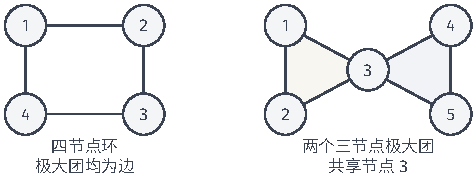
\includegraphics[width=80.652mm]{figures/06-probabilistic-graphical-models/01-representation/tikz/pgm-undirected-cliques/figure.pdf}
  \caption{无向图中的团与邻接。左图的四条边分别构成极大团，整个环因缺少对角边而不构成团；右图的两个三角形为极大团，共享节点$3$。无向线段表示邻接，节点编号对应随机变量下标。}
  \label{fig:pgm-undirected-cliques}
\end{figure}

观察一组节点后，两侧之间若已没有剩余路径，就用条件独立描述两侧的概率关系。采用这种语义的模型称为\term{无向图模型}（undirected graphical model），也称\term{Markov随机场}（Markov random field, MRF）或Markov网络。第~\ref{sec:pgm-undirected-global-independence}节将对任意节点集合正式陈述这项全局要求。

同一张无向图可以配上不同的局部函数，得到不同的分布。图只规定相容分布必须遵守的独立性，是对一整类分布的约束；数值参数则决定相邻变量实际具有多强的依赖。需要强调的是，图的保证只是“不强制相关”：如果某条边对应的相互作用强度取成零，两端变量仍可能独立，这种图没有要求的额外独立性完全可以出现。反过来，图中不存在的路径所对应的独立关系，却是相容分布都必须满足的。此外，无向边首先描述概率相互作用，并不说明干预某一端会如何改变另一端的分布；干预后的因果问题需要额外的因果建模语义，不能直接从无向边读出。这里采用的分离与Markov语义见无向图模型的标准表述\scite{pgm-lauritzen1996}。

\section{无向图的局部独立性}
\label{sec:pgm-undirected-local-independence}

在四节点环中，可以从两个不同粒度提出独立性问题。最直接的一种是盯住一条缺边：既然$1$与$3$之间没有边，那么在其余变量都已知的条件下，它们是否独立？这给出成对Markov性质。另一种是盯住一个节点：要预测$X_1$，需要知道哪些节点的取值，知道哪些之后其余节点就不再提供新信息？这给出局部Markov性质。两种问法涉及的独立侧和条件侧都不同，一个只处理一对节点，一个把一个节点与全部非邻居整体比较。它们看似相近，强弱却不完全相同，本节先分别建立这两种性质并讨论它们的关系，第~\ref{sec:pgm-undirected-global-independence}节再说明怎样由这些局部要求恢复任意集合之间的全局独立性。

\subsection{成对Markov性质}
\label{sec:pgm-undirected-pairwise}

两个非邻接节点$i,j$仍可能经其他节点相连。在环中$1$与$3$没有边，却同时经由$2$和$4$联系；若什么都不给定，两者的取值通常相关。成对Markov性质的想法是：把连接它们的所有中间节点全部给定，让每一条间接路径都被屏蔽，此时再要求这两个非邻接变量条件独立。条件侧取“其余全部节点”，正是为了不漏掉任何一条仍能传递信息的路径。

\begin{definition}[成对Markov性质]
  \label{def:pgm-undirected-pairwise}
  联合分布$p$相对于$\mathcal{G}$满足\term{成对Markov性质}（pairwise Markov property），是指对每一对不同且不相邻的节点$i,j$，都有
  \begin{equation}
    X_i\perp X_j\mid\bm{X}_{V\setminus\{i,j\}}.
    \label{eq:pgm-undirected-pairwise}
  \end{equation}
\end{definition}

四节点环中的非邻接对为$\{1,3\}$和$\{2,4\}$，对应的成对约束为
\[
  X_1\perp X_3\mid(X_2,X_4),
  \qquad
  X_2\perp X_4\mid(X_1,X_3).
\]
第一项同时以$X_2,X_4$为条件，这两个节点分别位于两条连接路径上。只给定$X_2$时，路径$1-4-3$仍然存在，结构尚未保证$X_1\perp X_3\mid X_2$。

这里需要区分离散与连续两种情形，因为它们“给定一个条件”的方式不同。对于离散变量，条件概率由概率的比值定义，只有在条件事件概率$p(\bm{x}_{V\setminus\{i,j\}})>0$时才有意义；二元条件独立就要求在这些正概率的条件配置下，条件联合概率等于两个条件边缘的乘积。若某个条件组合根本不会出现，对应的比值没有定义，自然也不能用同一比值去约束它。连续变量取特定值的概率通常为零，无法再用事件概率作比，因此改用条件密度或正则条件分布来表述，等式按条件变量的分布几乎处处成立；其严格依据与离散情形依赖正概率单点的论证并不相同。

成对性质便于按缺边列出约束，而集合查询还要同时处理多个变量。将一些已给定的变量移回未知侧会改变条件分布，因而从成对约束得到较大集合的独立性，需要相应的概率运算规则。后面的弱并与交性质将分别处理两种集合变化。

\subsection{局部Markov性质}
\label{sec:pgm-undirected-local}

现在换一种问法：固定一个节点$i$，想知道预测它时最少需要观测谁。从$i$出发到任何非邻居的路径，第一步都必须经过它的某个邻居$N(i)$；不经过邻居，就无法沿边走到图的其他部分。因此，一旦把全部邻居的值给定，$i$与所有非邻居之间的图上通道都被挡住。局部Markov性质把这一图上的屏蔽翻译成概率上的条件独立：给定邻居后，$X_i$与其余所有非邻居联合独立。

\begin{definition}[局部Markov性质]
  \label{def:pgm-undirected-local}
  联合分布$p$相对于$\mathcal{G}$满足\term{局部Markov性质}（local Markov property），是指对每个$i\in V$，都有
  \begin{equation}
    X_i\perp\bm{X}_{V\setminus(\{i\}\cup N(i))}
       \mid\bm{X}_{N(i)}.
    \label{eq:pgm-undirected-local}
  \end{equation}
\end{definition}

给定某个节点集合后，若$X_i$与集合以外的其他变量独立，形象地说这个集合像一层“毯子”把$X_i$与外部隔开，就称为$X_i$的\term{Markov毯}（Markov blanket）。满足局部Markov性质时，邻居集合$N(i)$就是图所保证的一层毯：知道邻居后，再知道任何更远的节点都不会改变对$X_i$的判断。图~\ref{fig:pgm-undirected-markov-blanket}以中心、邻居和远端节点三层展示这一结构：所有通向远端的路径都先经过邻居。

\begin{figure}[htbp]
  \centering
  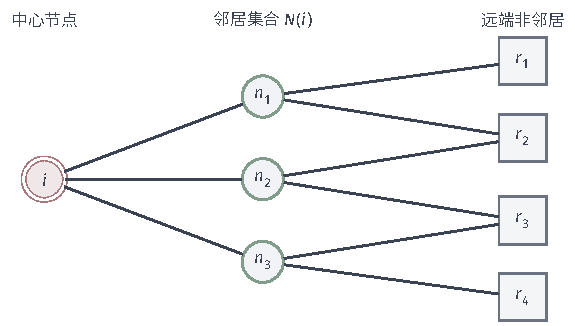
\includegraphics[width=97.402mm]{figures/06-probabilistic-graphical-models/01-representation/tikz/pgm-undirected-markov-blanket/figure.pdf}
  \caption{邻居集合构成的图上Markov毯。双边框圆为中心节点$i$，单边框圆为邻居$n_1,n_2,n_3$，方形为远端非邻居。实线均表示现存的无向边，中心到远端的每条路径先经过$N(i)$中的节点。}
  \label{fig:pgm-undirected-markov-blanket}
\end{figure}

在相应条件分布有定义的取值上，给定全部其他变量与只给定邻居得到相同的局部分布：
\begin{equation}
  p(x_i\mid\bm{x}_{V\setminus\{i\}})
  =p(x_i\mid\bm{x}_{N(i)}).
  \label{eq:pgm-undirected-blanket}
\end{equation}
该式把局部Markov性质落成一个可直接使用的结论：要计算某个节点在给定其余全部节点时的条件分布，只需查看它的邻居，远端节点的取值可以忽略。这正是后面许多局部计算（例如逐节点采样）只需邻居信息的根据。不过$N(i)$只是图在一般情况下保证的一层毯；对某个具体分布$p$，参数上的冗余可能允许更小的毯，例如某个邻居实际上从不改变局部分布，就可以把它省去。还要注意，即使图含有环，邻居仍然能屏蔽离开$i$的所有路径——因为任何这样的路径第一步必经过邻居，与后面是否绕成环无关，所以这项结构保证始终成立。

\begin{figure}[htbp]
  \centering
  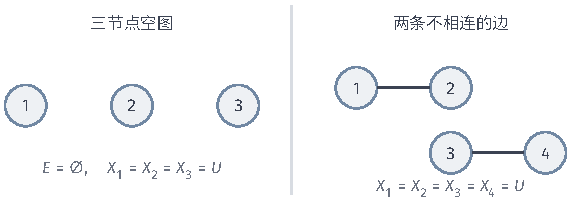
\includegraphics[width=96.686mm]{figures/06-probabilistic-graphical-models/01-representation/tikz/pgm-undirected-markov-counterexamples/figure.pdf}
  \caption{检验Markov性质逆向蕴含的两张图。各节点变量都等于同一个公平二值变量$U$，联合分布只有两个正概率配置。左侧空图满足成对性质而不满足局部性质；右侧两条不相连的边满足局部及成对性质而不满足全局性质。}
  \label{fig:pgm-undirected-markov-counterexamples}
\end{figure}

局部性质的结论强于成对性质：局部性质只给定邻居，却要求$X_i$与全部非邻居联合独立；成对性质给定其余全部节点，只要求其中一对独立。对一般分布，仅凭成对性质推不出局部性质，需要用退化分布说明；反过来，局部性质总能推出成对性质。

\begin{example}[成对性质不蕴含局部性质]
  \label{ex:pgm-undirected-pairwise-not-local}
  在图~\ref{fig:pgm-undirected-markov-counterexamples}左侧的三节点空图中，采用公平Bernoulli变量$U$，将三个节点都设为它的副本：
  \[
    X_1=X_2=X_3=U.
  \]
  空图的三对节点均不相邻，对应的全部成对约束是
  \[
    X_1\perp X_2\mid X_3,\qquad
    X_1\perp X_3\mid X_2,\qquad
    X_2\perp X_3\mid X_1.
  \]
  对第一项，在给定$X_3=u$的正概率事件下，两个未知变量也被确定为$u$。因此，对任意$u,a,b\in\{0,1\}$有
  \[
    \begin{aligned}
      p(X_1=a,X_2=b\mid X_3=u)
      &=\mathbf{1}\{a=u\}\mathbf{1}\{b=u\}\\
      &=p(X_1=a\mid X_3=u)p(X_2=b\mid X_3=u).
    \end{aligned}
  \]
  将$(X_1,X_2;X_3)$分别换为$(X_1,X_3;X_2)$和$(X_2,X_3;X_1)$，其余两项具有同样的指标函数乘积。三个成对约束由此全部成立。

  节点$1$的邻居集合$N(1)=\varnothing$，局部性质因而要求边缘独立$X_1\perp(X_2,X_3)$。比较全零状态的联合概率与边缘乘积，得到
  \[
    p\bigl(X_1=0,(X_2,X_3)=(0,0)\bigr)=\tfrac12
    \neq
    p(X_1=0)p\bigl((X_2,X_3)=(0,0)\bigr)=\tfrac14.
  \]
  两边分别为$1/2$和$1/4$，所以局部性质失败。分布只在$(0,0,0)$与$(1,1,1)$上为正，给定一个副本可以完全确定其他副本，而消去这个条件后，变量仍共同随$U$变化。这说明成对约束与无条件集合独立在当前支持集下有不同含义。
\end{example}

\begin{theorem}[局部Markov性质蕴含成对Markov性质]
  \label{thm:pgm-undirected-local-to-pairwise}
  设$\mathcal{G}=(V,E)$为有限简单无向图，$p$为节点随机变量$\bm{X}=(X_i)_{i\in V}$的任意联合分布。若$p$相对于$\mathcal{G}$满足局部Markov性质，则它满足成对Markov性质；该结论不要求$p$严格为正。
\end{theorem}

\begin{proof}
取一对任意不相邻节点$i,j$，并将$i$的非邻居记为$R=V\setminus(\{i\}\cup N(i))$，其中$j\in R$。由局部性质得到
\[
  X_i\perp\bm{X}_R\mid\bm{X}_{N(i)}.
\]
为了只保留$j$作为独立侧，需要把其余非邻居从独立侧移入条件集合。\term{弱并}（weak union）正是允许这种移动的条件独立运算规则：如果$X$在给定$W$后与$(Y,Z)$整体独立，那么再额外知道$Z$后，$X$仍与$Y$独立——本来就无关的信息，多知道一部分不会使其变得有关。写成式子即
\[
  X\perp(Y,Z)\mid W
  \quad\Longrightarrow\quad
  X\perp Y\mid(W,Z).
\]
前提使$p(x\mid y,z,w)=p(x\mid w)$，再按$p(y\mid z,w)$汇总$y$，得到$p(x\mid z,w)=p(x\mid w)$。两式右侧相同，所以给定$(Z,W)$后，再给定$Y$仍保持$X$的分布。这里使用相应条件分布有定义的配置，连续情形按条件变量分布几乎处处成立；这一转换允许联合分布取零值。

将$R$分为$\{j\}$与$R\setminus\{j\}$，把后一部分通过弱并移入条件，便有
\[
  X_i\perp X_j
  \mid\bigl(\bm{X}_{N(i)},\bm{X}_{R\setminus\{j\}}\bigr).
\]
条件侧合并了邻居与$j$之外的非邻居，恰好是$V\setminus\{i,j\}$。所得独立式就是这对节点的成对Markov约束，任意非邻接对都可采用同样的步骤。
\end{proof}

局部性质以邻居为条件，联合约束全部非邻居；成对性质以其他全部节点为条件，只约束其中一对。四节点环的每个节点恰有一个非邻居，所以该图中两种式子重合。链$1-2-3-4$则呈现差别：节点$1$的局部式是$X_1\perp(X_3,X_4)\mid X_2$，而相应两条成对式为$X_1\perp X_3\mid(X_2,X_4)$和$X_1\perp X_4\mid(X_2,X_3)$。要由后两条合并出前一条，相当于把$X_3,X_4$从条件侧一起移到独立侧；上面的弱并只能把变量从独立侧移到条件侧，方向恰好相反，无法完成这一合并。这需要下一节的交性质，而交性质只在严格正等条件下成立，这也解释了为什么两种性质在一般分布下并不等价。

\section{无向图的全局独立性}
\label{sec:pgm-undirected-global-independence}

成对和局部性质都只处理“一个或一对节点”层面的独立，而实际查询往往涉及两组区域。在图~\ref{fig:pgm-undirected-cliques}右侧，两个三角形区域分别为$\{1,2,3\}$与$\{3,4,5\}$，共享节点$3$。设想已知共享区域$3$的标签，想知道左侧区域$\{1,2\}$与右侧区域$\{4,5\}$是否还相互影响——这正是图像分割中“知道交界处后，左右两块能否分别推断”的问题。它的两侧都含多个变量，不能只靠单节点的局部式回答，需要考察连接两组节点的全部路径。

\subsection{全局Markov性质}
\label{sec:pgm-undirected-global}

左右两组节点被观测集合隔开时，所需结论是两组随机向量条件独立。\term{全局Markov性质}（global Markov property）把“路径阻断”这一图上事实统一翻译成概率约束：只要连接$A$与$B$的每一条路径都经过$S$中的某个节点，给定$\bm{X}_S$后两组变量就条件独立。它允许$A$、$B$是任意节点集合，$S$是任意能挡住全部路径的集合，因而前面的成对、局部性质都可以看作它在取特定集合时的特例。

\begin{definition}[全局Markov性质]
  \label{def:pgm-undirected-model}
  设$p$为$\bm{X}=(X_1,\ldots,X_d)^{\top}$的联合分布。若对任意两两不交的节点集合$A,B,S\subseteq V$，只要从任意$a\in A$到任意$b\in B$的每条路径都经过$S$中的节点，就有
  \begin{equation}
    \bm{X}_A\perp\bm{X}_B\mid\bm{X}_S,
    \label{eq:pgm-undirected-global}
  \end{equation}
  则称$p$相对于$\mathcal{G}$满足全局Markov性质，$(\mathcal{G},p)$构成一个无向图模型。
\end{definition}

定义从路径阻断推出分布独立，具体参数还可以给出图中未记录的额外独立性。在两个三角形共享节点$3$的例子中，从$\{1,2\}$到$\{4,5\}$的每条路径都经过$3$，因此得到
\[
  (X_1,X_2)\perp(X_4,X_5)\mid X_3.
\]
给定$X_3$后，联合条件分布分成左侧和右侧两个二元分布。每一侧内部仍可保留依赖，例如$X_1,X_2$同处一个三节点团，当前分离查询没有将它们分开。

查询集合与条件集合还可以只覆盖部分节点，即$A\cup B\cup S\neq V$。只查询$X_1,X_5$并给定$X_3$时，$X_2,X_4$留在未查询、未观测侧，同一路径判据仍给出$X_1\perp X_5\mid X_3$。证明全局性质因此还需边缘化这些剩余变量，处理三个集合未覆盖全部节点的情形。

\begin{theorem}[全局Markov性质蕴含局部与成对Markov性质]
  \label{thm:pgm-undirected-global-implications}
  设$\mathcal{G}=(V,E)$为有限简单无向图，$p$为节点随机变量$\bm{X}=(X_i)_{i\in V}$的任意联合分布。若$p$相对于$\mathcal{G}$满足全局Markov性质，则它同时满足局部与成对Markov性质。换言之，不附加严格正性时总有
  \begin{equation}
    \text{全局Markov}
    \ \Longrightarrow\ \text{局部Markov}
    \ \Longrightarrow\ \text{成对Markov}.
    \label{eq:pgm-undirected-implication}
  \end{equation}
\end{theorem}

\begin{proof}
固定$i\in V$，考察它到非邻居的路径。每条路径离开$i$后的首个节点都属于$N(i)$，所以$N(i)$分离$\{i\}$与$V\setminus(\{i\}\cup N(i))$。对这三个集合应用全局Markov性质，得到
\[
  X_i\perp\bm{X}_{V\setminus(\{i\}\cup N(i))}
  \mid\bm{X}_{N(i)},
\]
这正是节点$i$的局部约束。对全部节点重复该步骤，$p$便满足局部性质，再由定理~\ref{thm:pgm-undirected-local-to-pairwise}得到成对性质。
\end{proof}

上面的推导只用到“路径必经过邻居”这一图上事实和条件独立的基本运算，没有对概率取零作任何限制，所以“全局$\Rightarrow$局部$\Rightarrow$成对”对任意分布都成立。自然要追问反方向：能否从较弱的成对、局部性质重建出较强的全局性质？如果能，三种表述就只是同一约束的不同写法；如果不能，就需要弄清缺了什么条件。下面考察图~\ref{fig:pgm-undirected-markov-counterexamples}右侧的两个连通分量，用一个退化分布看到反方向确实可能失效：它满足各节点的局部约束，却在两个不相连的分量之间保留了共同随机性。

\begin{example}[局部、成对均不蕴含全局]
  \label{ex:pgm-undirected-local-not-global}
  将边集设为$E=\{\{1,2\},\{3,4\}\}$，四个变量仍取同一个公平二值变量的值：
  \[
    X_1=X_2=X_3=X_4=U,
    \qquad U\sim\operatorname{Bernoulli}(\tfrac12).
  \]
  两条边分别给每个节点提供一个邻居，局部性质要求
  \[
  \begin{aligned}
    X_1&\perp(X_3,X_4)\mid X_2,&
    X_2&\perp(X_3,X_4)\mid X_1,\\
    X_3&\perp(X_1,X_2)\mid X_4,&
    X_4&\perp(X_1,X_2)\mid X_3.
  \end{aligned}
  \]
  第一项给定$X_2=u$后，其他变量也随之确定。因此，对任意$u,a,r_3,r_4\in\{0,1\}$有
  \[
  \begin{aligned}
    &p(X_1=a,X_3=r_3,X_4=r_4\mid X_2=u)\\
    &\quad=\mathbf{1}\{a=u\}
            \mathbf{1}\{r_3=u,r_4=u\}\\
    &\quad=p(X_1=a\mid X_2=u)
            p(X_3=r_3,X_4=r_4\mid X_2=u).
  \end{aligned}
  \]
  将条件变量依次换为$X_1,X_4,X_3$，单节点端点依次换为$X_2,X_3,X_4$，便得到其余三项相同的指标函数分解。每一项都在正概率条件事件上成立，因此四项局部约束均被满足。

  不相邻的节点对为$\{1,3\}$、$\{1,4\}$、$\{2,3\}$与$\{2,4\}$，对应成对约束为
  \[
  \begin{gathered}
    X_1\perp X_3\mid(X_2,X_4),\qquad
    X_1\perp X_4\mid(X_2,X_3),\\
    X_2\perp X_3\mid(X_1,X_4),\qquad
    X_2\perp X_4\mid(X_1,X_3).
  \end{gathered}
  \]
  在任一缺边$\{i,j\}$的查询中，其余两个变量的正概率条件取值均为$(u,u)$。给定这样的取值后，
  \[
    p(X_i=a,X_j=b\mid\bm{X}_{V\setminus\{i,j\}}=(u,u))
    =\mathbf{1}\{a=u\}\mathbf{1}\{b=u\}.
  \]
  两个指标函数分别是条件边缘概率，故该式验证了四项成对独立。

  两个分量之间原本没有路径，全局性质要求$(X_1,X_2)\perp(X_3,X_4)$。然而它们共同随$U$变化，例如
  \[
    p(X_1=0,X_3=0)=\tfrac12
    \neq p(X_1=0)p(X_3=0)=\tfrac14.
  \]
  两个向量若独立，其分量$X_1,X_3$也应独立。上式的联合概率与边缘乘积不同，因此这个分布违背全局性质。
\end{example}

这两个反例能成立，关键都在于条件变量一旦给定，未知状态就被唯一确定，此时条件独立在一个退化为单点的条件分布上“平凡地”成立，它对其余取值组合没有任何约束力。逐变量的成对约束因此无法拼接成更大集合的独立。若要求完整乘积状态空间上的每一个配置都严格为正，任何条件组合就都真正可能发生，每一项条件独立都能在全部相关取值上使用，这就为合并这些约束提供了充分条件。

合并时需要一条与弱并方向相反的概率运算规则——交性质。设各坐标状态集有限且非空，并要求联合质量在完整乘积空间的每个配置上严格为正。对两两不交的索引集$A,B,C,D$，合并时使用的两个前提为
\[
  \bm{X}_A\perp\bm{X}_B\mid(\bm{X}_C,\bm{X}_D),
  \qquad
  \bm{X}_A\perp\bm{X}_D\mid(\bm{X}_C,\bm{X}_B).
\]
前一项表示给定$C,D$后，再知道$B$对$X_A$没有影响；后一项表示给定$C,B$后，再知道$D$对$X_A$也没有影响。交性质把两者合并为更强的结论：只给定$C$时，$X_A$与$(B,D)$整体都独立，即
\[
  \bm{X}_A\perp(\bm{X}_B,\bm{X}_D)\mid\bm{X}_C.
\]
与弱并相反，这条合并并不是无条件成立的——它要求$B$与$D$的每种组合都能在给定$C$时真正出现，否则“分别独立”的信息无法叠加；严格正性恰好排除了那种条件一给、其余状态就被锁死的退化情形，保证两组条件变量的每种组合都能作为条件，因而可以进行这种合并。这里使用的概率规则及其严格正条件，可参考\BookChapterRef{chap:random-variables}{卷2《数学准备：概率、因果与决策》的“随机变量与概率基础”章}。

在上述严格正的有限离散分布中，可以反复使用交性质，将逐变量的独立合并为集合独立。设$A,C,Y\subseteq V$两两不交，非空集合$Y=\{y_1,\ldots,y_m\}$；已知对每个$y_k$都有$\bm{X}_A\perp X_{y_k}\mid(\bm{X}_C,\bm{X}_{Y\setminus\{y_k\}})$。每项都把其他$Y$变量作为条件，合并的目标则是把全部$Y$移到独立侧。

令$D_0=\varnothing$、$D_k=\{y_1,\ldots,y_k\}$、$T_k=Y\setminus D_k$，分别记录已经合并和仍留在条件侧的节点。$k=1$时，原前提就是$\bm{X}_A\perp\bm{X}_{D_1}\mid(\bm{X}_C,\bm{X}_{T_1})$。对$k\geq2$，假设已经得到$\bm{X}_A\perp\bm{X}_{D_{k-1}}\mid(\bm{X}_C,X_{y_k},\bm{X}_{T_k})$，再将$y_k$的原前提写为$\bm{X}_A\perp X_{y_k}\mid(\bm{X}_C,\bm{X}_{D_{k-1}},\bm{X}_{T_k})$。这两项分别在另一侧给定的条件下独立，交性质将它们合成$\bm{X}_A\perp\bm{X}_{D_k}\mid(\bm{X}_C,\bm{X}_{T_k})$。

每一步使$D_k$增加一个节点、$T_k$减少一个节点。到$T_m=\varnothing$时，全部待合并变量已经进入独立侧，得到$\bm{X}_A\perp\bm{X}_Y\mid\bm{X}_C$。下面将对分离集两侧各应用一轮这种操作。

\begin{theorem}[严格正条件下三种Markov性质等价]
  \label{thm:pgm-undirected-markov-equivalence}
  设$\mathcal{G}=(V,E)$为有限简单无向图，每个节点$i\in V$对应取值于有限非空状态空间$\mathcal{X}_i$的随机变量$X_i$。令$p$为$\bm{X}=(X_i)_{i\in V}$在乘积状态空间$\mathcal{X}=\prod_{i\in V}\mathcal{X}_i$上的联合质量函数，并且$p(\bm{x})>0$对所有$\bm{x}\in\mathcal{X}$成立。则$p$相对于$\mathcal{G}$的成对、局部与全局Markov性质等价。
\end{theorem}

\begin{proof}
定理~\ref{thm:pgm-undirected-global-implications}给出了“全局$\Rightarrow$局部$\Rightarrow$成对”，所以剩余任务是由成对性质证明全局性质。取被$S$分离的非空集合$A,B$，在$\mathcal{G}[V\setminus S]$中，将与$A$相交的连通分量合为$U$，其余节点记为$W=V\setminus(S\cup U)$。于是$A\subseteq U$、$B\subseteq W$，且$U,W$之间没有边。先证明这两个较大集合条件独立，再缩到查询集合。

固定$u\in U$，它与每个$w\in W$都不相邻，因此成对性质给出
\[
  X_u\perp X_w
  \mid
  \bigl(\bm{X}_S,\bm{X}_{U\setminus\{u\}},
        \bm{X}_{W\setminus\{w\}}\bigr).
\]
第一轮以$Y=W$为待合并集合，以$C=S\cup(U\setminus\{u\})$为固定条件基集。使用上面的交性质步骤，把$W$逐节点移入独立侧，得到
\[
  X_u\perp\bm{X}_W
  \mid\bigl(\bm{X}_S,\bm{X}_{U\setminus\{u\}}\bigr).
\]
这个结论对每个$u\in U$成立。利用对称性，写成$\bm{X}_W\perp X_u\mid(\bm{X}_S,\bm{X}_{U\setminus\{u\}})$，便可取$Y=U$、条件基集$C=S$进行第二轮合并，得到$\bm{X}_W\perp\bm{X}_U\mid\bm{X}_S$。最后以对称性和分解性质保留$A,B$，得到$\bm{X}_A\perp\bm{X}_B\mid\bm{X}_S$，完成任意分离查询的证明。
\end{proof}

前面的两个反例都只保留两个完整配置：三节点例子由共同$U$确定，两分量例子只取$(0,0,0,0)$或$(1,1,1,1)$。交性质所需的其他条件组合在这些支持集上缺失，所以逐项条件独立无法按同样的步骤合并。严格正性保证合并可行，为三种性质的逆向蕴含提供了充分条件；各性质本身仍适用于一般分布。

\subsection{图分离的定义}
\label{sec:pgm-undirected-separation}

前面反复使用“每条路径都经过$S$”这一判据，现在把它固化成一个纯粹的图论概念，使结构判断不必每次都口头描述路径。最直观的检验方式是删除节点：把条件节点$S$连同与它们相连的边从图中删掉，若此时$A$与$B$之间不再有任何连通路径，就称$S$分离了$A$和$B$。这与“原图中从$A$到$B$的每条路径都经过$S$”完全等价——被删掉的节点正是原路径无法绕行的关卡。本章随后用全局Markov性质把这个结构判据连接到概率独立。

无向路径的内部节点只需检查是否属于条件集合，属于$S$的节点阻断所有经过它的路径。这个规则比第~\ref{chap:pgm-directed}章中需要区分碰撞与非碰撞位置的规则简单，但仍要检查全部连接路径，其他未阻断路径也能维持图上的连通。

图~\ref{fig:pgm-undirected-separation}分别删除四节点环中的$S=\{2\}$和$S=\{2,4\}$。前者留下$1-4-3$，后者把$\{1\}$与$\{3\}$分开。条件集合若继续扩大而保持与$A,B$不交，删除更多节点只会减少路径，所以图分离具有单调性。这里比较的是图上剩余路径，一般分布的条件独立运算还需自己的概率依据。

\begin{figure}[htbp]
  \centering
  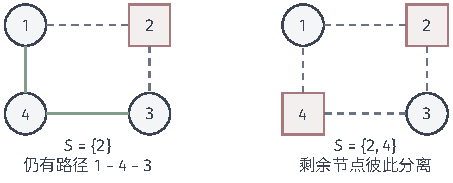
\includegraphics[width=76.652mm]{figures/06-probabilistic-graphical-models/01-representation/tikz/pgm-undirected-separation/figure.pdf}
  \caption{四节点环上的删除检测。方形节点属于条件集合$S$，与它们相接的虚线边一起删除，其余实线边保留。左侧只删$2$，仍可沿$1-4-3$连接；右侧删$2,4$，使$1,3$进入不同连通分量。}
  \label{fig:pgm-undirected-separation}
\end{figure}

\subsection{图分离的检测}
\label{sec:pgm-undirected-separation-test}

删除节点的判据虽然直观，但对有几十上百个节点的图，靠肉眼逐条数路径既慢又容易遗漏，因此需要一个确定的算法把“是否还连通”自动判定出来。做法正是在删去$S$后的诱导子图$\mathcal{G}[V\setminus S]$中，从$A$的全部节点出发搜索：从$A$的全部节点启动广度优先搜索，即可检查剩余连通性。搜索若到达$B$中的节点，就找到一条避开$S$的路径，说明未被分离；若搜索结束仍未到达$B$，则$S$构成分离集。每次扩张都沿保留的节点和边进行，所以访问集恰好覆盖与$A$有剩余路径的节点，这给出算法的正确性依据。采用邻接表和标记数组时，最坏时间为$O(d+|E|)$，额外空间为$O(d)$。这一开销针对结构查询，只回答“路径是否存在”；概率数值计算还要另外处理模型的局部函数与状态汇总。

\subsection{图分离的可靠性与模型类完备性}
\label{sec:pgm-undirected-separation-soundness-completeness}

图分离需要与概率独立严格对应，这种对应包含两个相反方向。\termalias{pgm-soundness}{可靠性}（soundness）要求图上读出的分离对所有按该图构造的分布都保证独立：只要$S$分离$A,B$，相容分布类中的每个分布都满足$\bm{X}_A\perp\bm{X}_B\mid\bm{X}_S$。\term{完备性}（completeness）则要求，对每一项未分离的查询，都至少存在一个相容分布让两端表现出依赖，这样的分布称为依赖见证。两个方向都成立时，图分离恰好刻画模型类强制的独立性：分离的一定独立，未分离的确实可能相关。具体参数仍可能产生图未强制的额外独立；完备性只保证存在依赖的分布，不保证每个分布都依赖。

为了说明具体参数如何带来额外独立，需要先构造由局部权重组成的分布。有向边有明确方向，每个局部表是给定父节点后的条件概率，可以逐行归一化为$1$；无向边没有方向，不能把一条边的一端说成条件于另一端，局部表也不能单独解释成条件分布。无向模型给局部变量组合的状态指定非负权重，所得函数称为\term{势函数}（potential function），简称势。势表达局部取值的相容程度，自身不要求是概率：值越大表示越相容，取$0$表示该局部组合被禁止。将一个完整配置涉及的各团权重相乘，得到未归一化总权重；再除以全部配置的权重总和得到概率。有限离散情形下，这个总和称为\term{配分函数}（partition function）$Z$，要求$Z>0$且有限；归一化由全局总和统一完成，单个局部势只记录相对权重。下面用常数势产生图未要求的独立性。

\begin{example}[不分离不强迫固定分布相关]
  \label{ex:pgm-undirected-fixed-distribution-extra-independence}
  考虑节点集$V=\{1,2\}$、边集$E=\{\{1,2\}\}$的无向图，并令$X_1,X_2\in\{-1,+1\}$。在唯一的二节点团上取常数边势
  \[
    \psi_{\{1,2\}}(x_1,x_2)=1.
  \]
  常数势给四个完整配置同样的权重$1$，总权重为$Z=1+1+1+1=4$。于是各配置的概率都是$p(x_1,x_2)=1/4$，得到一个严格正的联合分布。两个变量各自均匀取值，故对任意$x_1,x_2$，
  \[
    p(x_1,x_2)=\frac14
    =\frac12\cdot\frac12
    =p(x_1)p(x_2),
  \]
  即$X_1\perp X_2$。图中的边保留了两端发生相互作用的可能，常数势却没有使用这种相互作用。因而空集虽然无法分离两个端点，这组参数仍使二者独立。完备性要回答的是同一模型类中能否找到使二者依赖的参数；这个均匀分布只说明，选定参数可以带来图结构之外的独立性。
\end{example}

\begin{theorem}[团因子分解分布上的分离可靠性]
  \label{thm:pgm-undirected-factorization-to-global}
  设$\mathcal{G}=(V,E)$为有限简单无向图，节点$i\in V$取值于可测空间$(\mathcal{X}_i,\mathcal{A}_i)$，其上给定$\sigma$有限基准测度$\mu_i$；记$\mathcal{X}=\prod_{i\in V}\mathcal{X}_i$及$\mu=\bigotimes_{i\in V}\mu_i$，有限离散情形取计数测度。令$\mathcal{C}$为$\mathcal{G}$的有限团族，且对每个$C\in\mathcal{C}$，$\psi_C:\mathcal{X}_C\to[0,\infty)$是可测函数，其中$\mathcal{X}_C=\prod_{i\in C}\mathcal{X}_i$。若$p$相对于$\mu$的密度满足
  \[
    \begin{aligned}
      p(\bm{x})
      &=\frac{1}{Z}\prod_{C\in\mathcal{C}}\psi_C(\bm{x}_C)
        &&\text{$\mu$几乎处处},\\
      Z
      &=\int_{\mathcal{X}}\prod_{C\in\mathcal{C}}
        \psi_C(\bm{x}_C)\,\mathrm{d}\mu(\bm{x}),
        &&0<Z<\infty,
    \end{aligned}
  \]
  则对任意两两不交且$A,B$非空的$A,B,S\subseteq V$，若$S$在$\mathcal{G}$中分离$A$与$B$，就有
  \[
    \bm{X}_A\perp\bm{X}_B\mid\bm{X}_S.
  \]
  势函数可以取零，不要求$p$严格为正。
\end{theorem}

这个可靠性方向的证明要用到“联合分布由团势相乘构成”这一具体形式：图中的分离使团势落在条件集的两侧，分别归一化这两组势，再消去$A\cup B\cup S$以外的变量，就能得到条件概率的乘积。由于下一节才正式给出因子分解，完整证明放到第~\ref{sec:pgm-undirected-factorization-to-markov}节。下面先处理相反的完备性方向：沿一条未被阻断的路径构造依赖，证明模型类中确实存在使两端相关的分布。

\Needspace{14\baselineskip}
\begin{theorem}[严格正二值成对势模型类中的分离完备性]
  \label{thm:pgm-undirected-separation-completeness}
  设$\mathcal{G}=(V,E)$为有限简单无向图，每个节点$i\in V$对应二值随机变量$X_i\in\{-1,+1\}$，且$A,B,S\subseteq V$两两不交、$A,B$非空。若$S$在$\mathcal{G}$中不分离$A$与$B$，则存在一个严格正且按$\mathcal{G}$分解的成对势模型
  \[
    p(\bm{x})=\frac{1}{Z}
      \prod_{\{i,j\}\in E}\psi_{\{i,j\}}(x_i,x_j),
    \qquad \psi_{\{i,j\}}(x_i,x_j)>0,
  \]
  使$\bm{X}_A\not\perp\bm{X}_B\mid\bm{X}_S$。
\end{theorem}

\begin{proof}
从$A$到$B$存在一条避开$S$的路径；去掉路径中重复的节点，可取简单路径
\[
  v_0-v_1-\cdots-v_m,
  \qquad v_0\in A,\quad v_m\in B.
\]
取任意实数$J\neq0$。对路径上的边设
\[
  \psi_{\{v_{r-1},v_r\}}(x_{v_{r-1}},x_{v_r})
  =\exp(Jx_{v_{r-1}}x_{v_r}),
  \qquad r=1,\ldots,m,
\]
其余边的势取常数$1$。这样只让选定路径传递相互作用。所有势严格为正，状态空间有限，故$0<Z<\infty$，所得联合分布属于定理要求的模型类。

为了把这些边权写成转移概率，先固定前一节点的状态$a\in\{-1,+1\}$，对下一状态$b$求和：
\[
  \sum_{b\in\{-1,+1\}}\exp(Jab)
  =e^J+e^{-J}=2\cosh J,
  \qquad \cosh J=\frac{e^J+e^{-J}}{2}.
\]
这个和与$a$无关。对整条路径的权重求和时，可以先消去末端$v_m$，得到因子$2\cosh J$；再消去$v_{m-1}$，又得到同一个因子。依次消去$m$个末端变量后，只剩起点$v_0$的两种状态，所以路径总权重为$2(2\cosh J)^m$。因此
\[
  K(a,b)=\frac{\exp(Jab)}{2\cosh J}
\]
对每个$a$都满足$\sum_bK(a,b)=1$，可以作为下一状态的条件分布。以概率$1/2$选择起点，再逐步使用$K$，所得路径概率正好是原边势乘积除以它的总权重。这里的逐步归一化依赖这条特殊链及其与$a$无关的行和，不能推广为任意无向图上的各势独自归一化。

路径外的变量仅出现在常数势中，因而独立且均匀；连接路径内外的边也没有引入额外作用。完整联合分布由路径分布和路径外的均匀分布相乘得到。由于$\bm{X}_S$都位于路径外，给定它的取值后，路径分布保持原样：对每个$\bm{s}$，
\[
  p(x_{v_0},\ldots,x_{v_m}\mid\bm{s})
  =\frac12\prod_{r=1}^{m}
    \frac{\exp(Jx_{v_{r-1}}x_{v_r})}{2\cosh J}.
\]

把路径分布按相邻节点写成转移概率后，初始状态均匀，每一步都保留相同的耦合。为计算它在均值上的作用，记双曲正切
\[
  \tanh J=\frac{e^J-e^{-J}}{e^J+e^{-J}}.
\]
实数$J\neq0$使分子非零，因而$\rho=\tanh J\neq0$。固定前一状态$a$时，二值条件均值直接算为
\[
  \sum_{b\in\{-1,+1\}}bK(a,b)
  =a\frac{e^J-e^{-J}}{e^J+e^{-J}}
  =a\rho.
\]
所以相邻节点的条件均值满足
\[
  \mathbb{E}[X_{v_r}\mid X_{v_{r-1}}]
  =\rho X_{v_{r-1}}.
\]
转移核乘积还说明，给定$X_{v_0},\ldots,X_{v_{r-1}}$的整段历史后，下一状态的条件分布仍只依赖$X_{v_{r-1}}$。令$c_r=\mathbb{E}[X_{v_0}X_{v_r}]$，先对最后一个变量取条件期望，就有
\[
  \begin{aligned}
    c_r
    &=\mathbb{E}\!\left[
        X_{v_0}\mathbb{E}[X_{v_r}\mid
        X_{v_0},\ldots,X_{v_{r-1}}]\right]\\
    &=\rho\,\mathbb{E}[X_{v_0}X_{v_{r-1}}]
      =\rho c_{r-1}.
  \end{aligned}
\]
起点满足$c_0=\mathbb{E}[X_{v_0}^2]=1$，重复这一步便得到$c_m=\rho^m$。起点的均值为零，而$\mathbb{E}[X_{v_r}]=\rho\mathbb{E}[X_{v_{r-1}}]$，所以路径上各节点的均值也都为零。给定路径外的$\bm{X}_S$不改变这些矩。沿路径逐次取条件期望，每经过一条边便多乘一个耦合系数，因此得到
\[
  \mathbb{E}[X_{v_0}X_{v_m}\mid\bm{X}_S=\bm{s}]
  =\rho^m\neq0,
  \qquad
  \mathbb{E}[X_{v_0}\mid\bm{s}]
  =\mathbb{E}[X_{v_m}\mid\bm{s}]=0.
\]
两个端点的条件均值都是零，而乘积的条件均值非零，因此给定$\bm{X}_S$后仍有依赖。若$\bm{X}_A\perp\bm{X}_B\mid\bm{X}_S$，从两侧各取一个分量便应得到$X_{v_0}\perp X_{v_m}\mid\bm{X}_S$，与上述计算矛盾。选定的非零耦合由此提供了完备性所需的见证分布；换成零耦合，即$J$取零，同一张图也能表示独立分布。
\end{proof}

\section{无向图中的因子分解}
\label{sec:pgm-undirected-factorization}

给定一张无向图，相容的联合分布可以写成一组只依赖局部变量的小函数：图中缺边和分离约束变量间的依赖，具体配置的概率则由数值决定。无向图通过团上的非负权重描述局部相容关系，将这些权重相乘并做一次全局归一化后得到联合分布。这一表示引出两个方向的问题：若分布已经写成团上局部函数的乘积，它是否满足图读出的条件独立；反过来，若分布满足图的全部Markov独立性，是否总能找到这样一组团势表示它。本节先说明团势怎样组织与计算，再依次证明这两个方向，并检查逆向结论在零概率配置和连续变量上的成立条件。

\subsection{因子分解的定义}
\label{sec:pgm-undirected-factorization-definition}

沿用前面的局部权重，为图中每个选定团指定一个势：设$\mathcal{C}$是团的一个族，$\psi_C(\bm{x}_C)$是团$C$上的有限非负函数。将这些势相乘，若能找到$0<Z<\infty$使
\begin{equation}
  p(\bm{x})=\frac{1}{Z}\prod_{C\in\mathcal{C}}\psi_C(\bm{x}_C),
  \label{eq:pgm-undirected-factorization}
\end{equation}
则称$p$按照$\mathcal{G}$进行团因子分解。每个势的自变量来自一个团，实际取值可以只受其中部分变量影响；例如常数势完全不使用团内变量的状态。

势的乘积给出的是一组相对权重，还不是概率：所有配置的权重加起来一般不等于$1$。除以$Z$正是为了把它们等比例缩放成一个合法分布，使全部配置的概率之和为$1$；缩放不改变任意两个配置概率的比值。在离散状态空间上，归一化需要遍历完整配置，将相乘后的权重累加：
\begin{equation}
  Z=\sum_{\bm{x}\in\mathcal{X}}\prod_{C\in\mathcal{C}}\psi_C(\bm{x}_C),
  \qquad
  \mathcal{X}=\prod_{i\in V}\mathcal{X}_i.
  \label{eq:pgm-undirected-partition}
\end{equation}
有限状态空间上，这个有限和给出有限的$Z$；只要至少一个配置权重非零，便有合法的概率分布。可数无限状态空间还需要求和级数收敛。势$\psi_C$记录相对权重，其自身的总和可以异于$1$。不同团共享变量，局部各自归一化后，相乘的函数仍需要全局归一化常数$Z$。

可以用三个二值变量看清最后一点。取两个重叠团$\{1,2\}$与$\{2,3\}$，令两张势表的每项都为$1/4$。每张表按自己的四种配置求和均为$1$，但完整配置共有八种，每种配置的乘积权重为$1/16$，于是
\[
  \sum_{x_1,x_2,x_3}
    \psi_{\{1,2\}}(x_1,x_2)\psi_{\{2,3\}}(x_2,x_3)
  =8\cdot\frac{1}{16}=\frac12.
\]
共享的$x_2$在完整配置中只取一次值，不能把这个求和拆成两张表各自总和的乘积。本例仍需用$Z=1/2$归一化，最终八种配置的概率均为$1/8$。这里按整张团表归一化，与有向条件表在每个父配置下对子状态求和为$1$不同；后者才允许沿无环顺序逐层消去归一化因子。

全局归一化的代价取决于怎样组织求和。若$d$个变量各有$q$个状态，式~\eqref{eq:pgm-undirected-partition}的直接枚举要计算$q^d$项：$20$个二值变量就有$2^{20}=1048576$种配置。链、树或树宽较小的图能让不同配置共享部分计算，从而降低相对于枚举的开销；精确推断章节将说明如何利用这种结构。

全局归一化看似要求把所有配置的权重都算一遍，但有一类查询可以局部完成。给定其余所有变量、只问$X_i$的条件分布时，条件概率是$X_i$各取值权重的相对比值，全局$Z$会在比值中约掉。记未归一化权重为$w(\bm{x})=\prod_{C\in\mathcal C}\psi_C(\bm{x}_C)$，固定$\bm{x}_{-i}=\bm{x}_{V\setminus\{i\}}$，取$p(\bm{x}_{-i})>0$的条件事件。条件概率的分子与分母都带有同一个全局常数：
\begin{equation}
  \begin{aligned}
    p(x_i\mid\bm{x}_{-i})
      &=\frac{w(x_i,\bm{x}_{-i})/Z}
        {\sum_{a\in\mathcal X_i}w(a,\bm{x}_{-i})/Z}\\
      &=\frac{\prod_{C\ni i}\psi_C(\bm{x}_C)}
        {\sum_{a\in\mathcal X_i}
          \prod_{C\ni i}\psi_C(a,\bm{x}_{C\setminus\{i\}})}.
  \end{aligned}
  \label{eq:pgm-undirected-local-conditional}
\end{equation}
在这个比值中，$Z$和所有不含$i$的势都被约去，分母只保留涉及$X_i$的势。记号$\psi_C(a,\bm{x}_{C\setminus\{i\}})$表示将第$i$个变量置为$a$，其余坐标使用已给定的值。二值节点因此只需把两项权重归一化。这个简化利用了其余变量全部已知的条件；若只有少数证据，未观测变量仍需边缘化，通常会留下更大的求和。

任意团都包含于某个极大团，因此小团势可以乘入一个包含它的极大团势。给每个小团选择一次归属，就能将所有势整理为仅以极大团为索引的乘积，同时保持原来的联合分布。“按团分解”与“按极大团分解”由此表示同一分布族，参数组织可以不同。团的阶数则影响所能表示的作用：一般的三节点团势包含三者共同取值的影响，单点势与成对势的乘积未必能表示它。

当势严格为正时，取对数可以把“各团权重相乘”改写成“各项相加”，这在求导、做优化以及借用统计物理语言时都方便得多。令$\varepsilon_C=-\log\psi_C$（势越大，这个量越小），并定义\term{能量函数}（energy function）$E(\bm{x})=\sum_C\varepsilon_C(\bm{x}_C)$为各团“代价”之和，便有
\[
  p(\bm{x})=Z^{-1}\exp[-E(\bm{x})].
\]
指数形式将相乘的相容权重改为相加的能量，较低能量对应较大权重。零势可记作$\varepsilon_C=+\infty$，以表示被禁止的配置；后面需要计算有限对数差分的证明则限于严格正势。

连续变量将求和换成积分。指定各坐标上的$\sigma$有限基准测度$\mu_i$，联合基准测度为$\mu=\bigotimes_{i\in V}\mu_i$，实数变量通常取Lebesgue测度；这是第~\ref{sec:pgm-directed-factor-definition}节采用的密度约定。可测势的乘积需要满足
\begin{equation}
  0<Z=\int_{\mathcal{X}}\prod_{C\in\mathcal{C}}
       \psi_C(\bm{x}_C)\,\mathrm{d}\mu(\bm{x})<\infty.
  \label{eq:pgm-undirected-continuous-partition}
\end{equation}
有限且正的积分使式~\eqref{eq:pgm-undirected-factorization}成为归一化密度。这里检查的是整个势乘积：一些单独不可积的势相乘后可以可积，而$\mathbb{R}^d$上的正的常数势乘积仍会有无穷积分。后面的高斯参数化将用精度矩阵的正定性具体表达这项全局条件。

\begin{example}[四节点环上的相容分数]
  \label{ex:pgm-undirected-cycle}
  令$X_i\in\{0,1\}$，四条边上的势相同：
  \[
    \psi_{\{i,j\}}(x_i,x_j)=
    \begin{cases}
      2,&x_i=x_j,\\
      1,&x_i\neq x_j.
    \end{cases}
  \]
  两端状态相同的一条边将权重乘以$2$，不同的边保持权重。对图~\ref{fig:pgm-undirected-factorization-example}中的$\bm{x}=(0,0,1,1)$，四个边势的乘积是$4$，用$Z=82$归一化便得到概率$2/41$。为计算这个常数，将配置按相同边数分类：沿环回到起点时，状态改变次数为偶数，相同边数因此只能是$4,2,0$。表~\ref{tab:pgm-undirected-cycle-weights}据此汇总全部$16$种配置。
  三类权重相加给出$Z=32+48+2=82$。全相同配置的概率为$p(0,0,0,0)=16/82=8/41$，交替配置的概率为$p(0,1,0,1)=1/82$。相容势由此明确了各配置的相对概率；这些数值只用于演示指定势后的计算。
\end{example}

\begin{figure}[htbp]
  \centering
  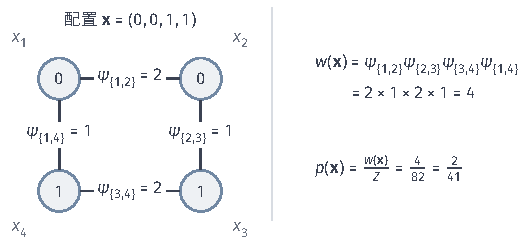
\includegraphics[width=89.701mm]{figures/06-probabilistic-graphical-models/01-representation/tikz/pgm-undirected-factorization-example/figure.pdf}
  \caption{四节点环中配置$\bm{x}=(0,0,1,1)$的权重与概率。四条边的势值相乘为$4$；全部$16$种配置的权重之和为$Z=82$，因此该配置的概率为$2/41$。}
  \label{fig:pgm-undirected-factorization-example}
\end{figure}

\begin{table}[htbp]
  \centering
  \begin{tabular}{crrr}
    \toprule
    相同边数 & 配置数 & 单个权重 & 总权重 \\
    \midrule
    $4$ & $2$ & $16$ & $32$ \\
    $2$ & $12$ & $4$ & $48$ \\
    $0$ & $2$ & $1$ & $2$ \\
    \bottomrule
  \end{tabular}
  \caption{按相同边数汇总四节点二值环的配置。相同边的势为$2$，不同边的势为$1$；各类总权重相加得到配分函数$82$。}
  \label{tab:pgm-undirected-cycle-weights}
\end{table}

\subsection{从因子分解到条件独立性}
\label{sec:pgm-undirected-factorization-to-markov}

删除分离集$S$后，图的连通分量将查询的两组节点隔开。团内节点两两相连，故一个团无法同时跨越这两侧。利用这一点整理团势，就能证明定理~\ref{thm:pgm-undirected-factorization-to-global}中的条件独立性。

\begin{proof}[定理~\ref{thm:pgm-undirected-factorization-to-global}的证明]
取两两不交且被$S$分离的$A,B,S$，其中$A,B$均非空。在$\mathcal{G}[V\setminus S]$中，将所有与$A$相交的连通分量合为$U$，其余节点合为$W=V\setminus(S\cup U)$。这些集合满足$A\subseteq U$、$B\subseteq W$，且$U$与$W$之间无边。

若一个团含有$U$和$W$各一个节点，两节点之间就应有边，这与集合的构造矛盾。因此每个团或者全部在$S$中，或者只涉及$U$与$S$，或者只涉及$W$与$S$。分别将这三类势相乘，联合分布写成
\begin{equation}
  p(\bm{u},\bm{w},\bm{s})
  =Z^{-1}h(\bm{s})f(\bm{u},\bm{s})g(\bm{w},\bm{s}),
  \label{eq:pgm-undirected-separated-factors}
\end{equation}
三组自变量$\bm{u},\bm{w},\bm{s}$分别对应$\bm{X}_U,\bm{X}_W,\bm{X}_S$；某类没有势时，其乘积取$1$。

为了将两侧函数归一化，在离散情形定义$F(\bm{s})=\sum_{\bm{u}}f(\bm{u},\bm{s})$、$G(\bm{s})=\sum_{\bm{w}}g(\bm{w},\bm{s})$；连续情形使用相应乘积测度的积分。取$p_S(\bm{s})$有限且严格为正的条件值，离散情形的所有正概率事件都满足此条件，连续情形中这样的取值承载全部$\bm{X}_S$概率。式~\eqref{eq:pgm-undirected-separated-factors}由此要求$h(\bm{s})$为正。团势非负，Tonelli定理允许先分别积分两侧函数，得到
\[
  p_S(\bm{s})=Z^{-1}h(\bm{s})F(\bm{s})G(\bm{s}).
\]
正且有限的条件密度排除了两侧积分为零或无穷的情形：$F(\bm{s})$或$G(\bm{s})$为零时联合积分为零，一侧积分无穷而另一侧为正时联合积分无穷。所以两侧的$F(\bm{s})$与$G(\bm{s})$均正且有限，条件联合密度成为
\begin{equation}
  p(\bm{u},\bm{w}\mid\bm{s})
  =\frac{f(\bm{u},\bm{s})}{F(\bm{s})}
   \frac{g(\bm{w},\bm{s})}{G(\bm{s})}.
  \label{eq:pgm-undirected-conditional-product}
\end{equation}
右侧各因子分别是两侧的条件密度，这个乘积给出$\bm{X}_U\perp\bm{X}_W\mid\bm{X}_S$。

最后分别消去$U\setminus A$和$W\setminus B$的变量。式~\eqref{eq:pgm-undirected-conditional-product}的两侧仍可独立求和或积分，留下只含$\bm{x}_A,\bm{s}$和只含$\bm{x}_B,\bm{s}$的条件边缘分布。故$\bm{X}_A\perp\bm{X}_B\mid\bm{X}_S$，任意被分离的两组变量都满足所需条件独立性。
\end{proof}

两侧函数的归一化在正概率条件事件或几乎处处的条件密度上完成，所除的常数正且有限。因此团势中的零值也适用于此证明。再结合定理~\ref{thm:pgm-undirected-global-implications}，团分解同时推出局部和成对性质。这个方向直接来自势乘积；下一节的Hammersley--Clifford结论负责相反方向，即从独立性重建团势。

对四节点环，可以直接看到这种两侧归一化。固定示例~\ref{ex:pgm-undirected-cycle}中的$X_2=x_2,X_4=x_4$，将涉及节点1和节点3的边势各自相乘：
\[
  \begin{aligned}
    f(x_1)&=\psi_{\{1,2\}}(x_1,x_2)\psi_{\{1,4\}}(x_1,x_4),\\
    g(x_3)&=\psi_{\{2,3\}}(x_2,x_3)\psi_{\{3,4\}}(x_3,x_4).
  \end{aligned}
\]
两邻居都取零时，即$x_2=x_4=0$，两侧权重满足$f(0)=g(0)=4$和$f(1)=g(1)=1$，因而
\[
  p(x_1,x_3\mid0,0)
  =\frac{1}{25}
    \begin{pmatrix}16&4\\4&1\end{pmatrix}_{x_1+1,x_3+1}.
\]
行与列都按状态$0,1$排列。两侧的条件边缘均为$(4/5,1/5)$，相乘正好得到矩阵的各项。若换成$x_2=0,x_4=1$，$f$与$g$的两种状态权重都为$2$，四个条件联合概率便都为$1/4$。两种条件值产生不同的边缘分布，但每种情况下，给定邻居后的联合分布都由两侧边缘相乘得到。

\subsection{从条件独立性到因子分解}
\label{sec:pgm-undirected-hammersley-clifford}

正向（团乘积$\Rightarrow$独立性）相对直接，逆向（独立性$\Rightarrow$团乘积）则更微妙，也是无向图模型理论的核心：现在只知道联合分布满足图的全部独立性约束，需要为它找到一组团势。构造的思路可以先从直觉上理解：先任意选定一个基准配置作为参照，考察把其中一部分坐标改成当前取值时，对数概率改变了多少；这个改变量原则上可能依赖被改变的任意一组变量。若某一组变量中包含两个在图上不相邻的节点，缺边所要求的条件独立就会保证“它们的联合改变没有额外贡献”，对应的交互项必然为零。于是能留下非零贡献的变量组，恰好都是两两相连的团。下面用Gill笔记中的Möbius交替差分把这一构造严格完成\scite{pgm-undirected-gill2011}。

\term{Hammersley--Clifford定理}在有限离散、严格正的情形下给出独立性与团分解的等价关系。严格正的范围是完整的笛卡尔积$\mathcal{X}=\prod_i\mathcal{X}_i$：每个配置都须满足$p(\bm{x})>0$，范围覆盖各坐标状态组合出的全部配置。定理~\ref{thm:pgm-undirected-markov-equivalence}已证明三种Markov性质在这些条件下等价，所以只需从其中一种构造团势。

\begin{theorem}[有限离散Hammersley--Clifford定理]
  \label{thm:pgm-undirected-hammersley-clifford}
  设$\mathcal{G}=(V,E)$为有限简单无向图，每个节点$i\in V$对应取值于有限非空状态空间$\mathcal{X}_i$的随机变量$X_i$。令$p$为$\bm{X}=(X_i)_{i\in V}$在乘积状态空间$\mathcal{X}=\prod_{i\in V}\mathcal{X}_i$上的联合质量函数，并且$p(\bm{x})>0$对所有$\bm{x}\in\mathcal{X}$成立。则以下四个条件等价：$p$满足相对于$\mathcal{G}$的全局Markov性质；$p$满足相对于$\mathcal{G}$的局部Markov性质；$p$满足相对于$\mathcal{G}$的成对Markov性质；$p$能按$\mathcal{G}$的团分解。分解中的势可以全部取为严格正值。
\end{theorem}

\begin{proof}
团分解到全局性质的方向由定理~\ref{thm:pgm-undirected-factorization-to-global}给出，三种Markov性质的等价由定理~\ref{thm:pgm-undirected-markov-equivalence}给出。剩下的任务是从成对性质重建分布。任选基准配置$\bm{x}^{\circ}\in\mathcal{X}$，对每个$D\subseteq V$，记
\[
  \bm{x}^{D}=(\bm{x}_D,\bm{x}^{\circ}_{V\setminus D}),
  \qquad
  L_D(\bm{x}_D)=\log p(\bm{x}^{D}).
\]
配置只在$D$中的坐标使用当前值，其他坐标都取基准值。每个配置概率严格为正，所以这些对数可作为有限实数参与后面的加减。

改变一组变量$D$引起的对数概率变化，既可能来自这些变量各自的单独作用，也可能来自它们之间的交互作用。要单独留下“$D$中变量同时改变才产生”的那部分，就要把只改变其中更小子集时的贡献逐一扣掉：加回单变量项、再扣掉被多减的部分，如此交替进行，这正是容斥的做法。为分离出每个坐标子集的作用，对每个$D\subseteq V$构造
\begin{equation}
  \phi_D(\bm{x}_D)
  =\sum_{B\subseteq D}(-1)^{|D|-|B|}L_B(\bm{x}_B).
  \label{eq:pgm-undirected-mobius}
\end{equation}
常数项为$\phi_{\varnothing}=\log p(\bm{x}^{\circ})$。这种\term{Möbius分解}（Möbius decomposition）用交替加减剔除较小子集的作用，留下同时改变$D$中各坐标时额外产生的部分。单节点项和二节点项分别为
\[
  \begin{aligned}
    \phi_{\{i\}}&=L_{\{i\}}-L_{\varnothing},\\
    \phi_{\{i,j\}}
      &=L_{\{i,j\}}-L_{\{i\}}-L_{\{j\}}+L_{\varnothing}.
  \end{aligned}
\]

验证这些局部项是否保留了完整分布，可将所有$D$的项重新相加。交换两层有限求和，得到
\begin{align}
  \sum_{D\subseteq V}\phi_D(\bm{x}_D)
  &=\sum_{B\subseteq V}L_B(\bm{x}_B)
      \sum_{D:\,B\subseteq D\subseteq V}(-1)^{|D|-|B|}
      \notag\\
  &=L_V(\bm{x}_V)=\log p(\bm{x}).
  \label{eq:pgm-undirected-mobius-inversion}
\end{align}
为计算固定$B$对应的内层系数，将包含$B$的每个$D$唯一写成$D=B\cup K$，其中$K\subseteq V\setminus B$。此时$|D|-|B|=|K|$，而从$V\setminus B$中选出$k$个额外节点有$\binom{|V\setminus B|}{k}$种方式，所以
\[
  \begin{aligned}
    \sum_{D:\,B\subseteq D\subseteq V}(-1)^{|D|-|B|}
    &=\sum_{k=0}^{|V\setminus B|}
        \binom{|V\setminus B|}{k}(-1)^k\\
    &=(1-1)^{|V\setminus B|}.
  \end{aligned}
\]
$B\neq V$时，额外节点的子集所给出的正负项相消，该系数为零；$B=V$时只剩$K=\varnothing$对应的唯一一项$1$。因此最终仅保留完整配置的对数概率。

成对性质随后决定哪些局部项留下。非空子集$D$若不是团，其内就有不相邻节点$i,j$；令$R=V\setminus\{i,j\}$。固定任意$\bm{x}_R$时，两节点的条件联合概率由各自条件边缘相乘得到。对任意$a,a'\in\mathcal{X}_i$和$b,b'\in\mathcal{X}_j$，先在这个条件分布内比较四个取值：
\[
  \begin{aligned}
    &p(a,b\mid\bm{x}_R)p(a',b'\mid\bm{x}_R)\\
    &\quad=p(a\mid\bm{x}_R)p(a'\mid\bm{x}_R)
            p(b\mid\bm{x}_R)p(b'\mid\bm{x}_R)\\
    &\quad=p(a,b'\mid\bm{x}_R)p(a',b\mid\bm{x}_R).
  \end{aligned}
\]
两边的四个条件边缘因子完全相同，只是组合次序不同。每个条件联合概率乘以$p(\bm{x}_R)$就恢复联合概率，因此两侧同乘$p(\bm{x}_R)^2$，得到
\begin{equation}
  \begin{aligned}
    &p(a,b,\bm{x}_R)p(a',b',\bm{x}_R)\\
    &\qquad=p(a,b',\bm{x}_R)p(a',b,\bm{x}_R).
  \end{aligned}
  \label{eq:pgm-undirected-rectangle}
\end{equation}
也可以从联合概率除以$p(\bm{x}_R)$的条件化公式反向核对：两边的归一化因子相同，可以约去。严格正性使这个条件事件的概率为正。取$a=x_i,a'=x_i^{\circ},b=x_j,b'=x_j^{\circ}$，使$R$中一个子集$B$使用当前值，其余坐标使用基准值。取有限对数后，有
\[
  L_{B\cup\{i,j\}}-L_{B\cup\{i\}}
  -L_{B\cup\{j\}}+L_B=0.
\]
这个零差分说明，其他坐标固定时，两非邻居的联合变化可以完全由各自的变化解释。

令$T=D\setminus\{i,j\}$。在式~\eqref{eq:pgm-undirected-mobius}中，先固定$B\subseteq T$。原来求和中的四个子集是$B$、$B\cup\{i\}$、$B\cup\{j\}$和$B\cup\{i,j\}$；它们含有相同的其他节点，只在是否纳入$i,j$上不同。由于$|D|=|T|+2$，这四项在提出共同系数$(-1)^{|T|-|B|}$后，符号依次为$+,-,-,+$。因此按子集是否含有$i,j$将求和项分为四组，再把同一个$B$的四项放在一起，便对应刚才的矩形差分：
\begin{equation}
  \begin{aligned}
    \phi_D
    =\sum_{B\subseteq T}(-1)^{|T|-|B|}
      \bigl(&L_{B\cup\{i,j\}}-L_{B\cup\{i\}}\\
            &-L_{B\cup\{j\}}+L_B\bigr)=0.
  \end{aligned}
  \label{eq:pgm-undirected-nonclique-vanishes}
\end{equation}
每个括号都为零，故只要一个子集含有非邻接对，它的整个交互项就为零。这一步同时排除了涉及这对节点的所有更高阶项。

留下的非空子集全是团，记其族为$\mathcal{C}_{\mathrm{all}}$。令$\psi_C=\exp(\phi_C)>0$，将式~\eqref{eq:pgm-undirected-mobius-inversion}的和指数化，得到
\[
  p(\bm{x})
  =\exp(\phi_{\varnothing})
     \prod_{C\in\mathcal{C}_{\mathrm{all}}}\psi_C(\bm{x}_C).
\]
联合概率对$\bm{x}$求和为一，所以团势乘积的配分函数是$Z=\exp(-\phi_{\varnothing})$，正且有限。若需仅保留极大团，进一步将每个小团势并入一个包含它的极大团即可。
\end{proof}

Möbius恒等式负责重建对数概率，成对独立性负责消去非团项，两者共同给出团分解。严格正性使每个其余变量配置都能用于条件化，也使矩形等式的对数有限。这是逆向结论在整类分布上成立的充分条件。沿用四节点环，下面给出一个带零概率的分布：它满足所有Markov独立性，却无法按团分解，从而展示严格正性所保护的方向。

\begin{example}[满足全局Markov性质却不能团分解]
  \label{ex:pgm-undirected-zero-support}
  在同一四节点环上，用两个相互独立的公平二值变量$U,V$构造分布：
  \[
    X_1=U,\quad X_2=V,\quad
    X_3=U\mathbin{\oplus}V,\quad X_4=U,
  \]
  $\oplus$表示模$2$加法。两变量的四种取值分别生成表~\ref{tab:pgm-undirected-zero-support}中的四个配置，其他完整配置的概率均为零。
\end{example}

\begin{table}[htbp]
  \centering
  \begin{tabular}{ccccc}
    \toprule
    $x_1$ & $x_2$ & $x_3$ & $x_4$ & 概率 \\
    \midrule
    $0$ & $0$ & $0$ & $0$ & $1/4$ \\
    $0$ & $1$ & $1$ & $0$ & $1/4$ \\
    $1$ & $0$ & $1$ & $1$ & $1/4$ \\
    $1$ & $1$ & $0$ & $1$ & $1/4$ \\
    \bottomrule
  \end{tabular}
  \caption{四节点环中四个正概率配置。给定任意一对对角节点即可确定所在行；边上的取值对允许的组合则多于这个全局支持集。}
  \label{tab:pgm-undirected-zero-support}
\end{table}

先检验独立性。给定$(X_2,X_4)$便知道$(U,V)$，$X_1$与$X_3$都成为常量，所以二者条件独立。给定$(X_1,X_3)$也能确定$(U,V)$，从而$X_2\perp X_4\mid(X_1,X_3)$。四节点环删除一个节点仍连通，非空节点集间的非平凡分离只可能是用一对对角节点隔开另一对。这两项条件独立因此覆盖全局Markov性质要求的所有查询，局部和成对性质也随之成立。

再检验能否分解。假设已有四个边势，单点势可先乘入某个关联的边势。取零概率配置$\bm{y}=(0,0,1,0)$：边$\{1,2\}$的取值$(0,0)$在正概率配置$(0,0,0,0)$中出现；边$\{2,3\}$的取值$(0,1)$在$(1,0,1,1)$中出现；边$\{3,4\}$的取值$(1,0)$在$(0,1,1,0)$中出现；边$\{1,4\}$的取值$(0,0)$则又在$(0,0,0,0)$中出现。每个正概率配置都要求其边势乘积为正，所以上述四个边势值全部为正。在$\bm{y}$处相乘便会给出$p(\bm{y})>0$，与指定的零概率矛盾。

图~\ref{fig:pgm-undirected-zero-support}将这四个取值对标在环的边上。局部投影各自允许这些取值，拼成的完整配置却不属于表~\ref{tab:pgm-undirected-zero-support}的支持集。
\begin{figure}[htbp]
  \centering
  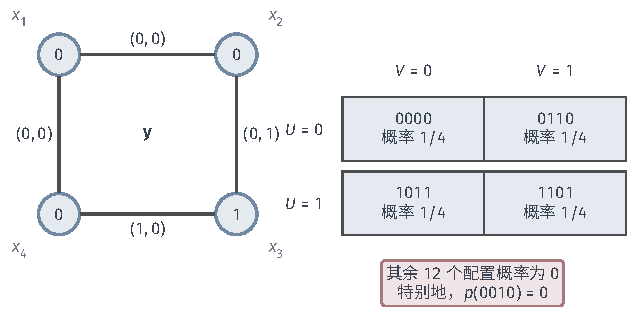
\includegraphics[width=106.825mm]{figures/06-probabilistic-graphical-models/01-representation/tikz/pgm-undirected-zero-support/figure.pdf}
  \caption{全局Markov性质成立而团分解失败的零概率反例。左侧配置$\bm y=(0,0,1,0)$的每个边取值对都出现在正概率配置中；右侧$2\times2$表按$(U,V)$列出四个正概率配置，其余12个配置的概率为0。边势若表示这些正概率配置，$\bm y$处的各势值也须为正，故无法同时满足$p(\bm y)=0$。}
  \label{fig:pgm-undirected-zero-support}
\end{figure}

这个分布的条件独立来自条件变量对其余变量的完全确定。其全局支持约束却超出了边势能表达的范围：四个局部允许的取值对可以拼成一个全局禁止的配置。上述矛盾直接排除了非负团势分解。零概率分布中也有可分解的情形，例如边势$\mathbf{1}\{x_i=x_j\}$能用局部零值施加相等约束；有零值时，逆向分解是否成立取决于具体支持结构。

对连续密度，基准配置构造还遇到逐点值的问题。若只知道$p>0$几乎处处，一个预先固定的坐标截面可能属于零测集，而密度在这样的集合上可任意修改。这会影响在截面上定义$L_D$的逐点推理。一般可测空间中的逆向定理需要处理这些例外集合及密度版本\scite{pgm-lauritzen1996}。

例如，在二维域$(0,1)^2$上取均匀密度$p(x_1,x_2)=1$，再选择下面这个版本：
\[
  \widetilde p(x_1,x_2)=
  \begin{cases}
    0,&x_2=1/2,\\
    1,&x_2\neq1/2.
  \end{cases}
\]
直线$x_2=1/2$的二维Lebesgue测度为零，所以两种密度给出同一个联合分布，且$\widetilde p>0$几乎处处。可是取基准配置$\bm{x}^{\circ}=(1/2,1/2)$、令$D=\{1\}$时，$\bm{x}^{D}=(x_1,1/2)$始终落在这条直线上。沿这个截面读取的$L_D=\log\widetilde p(x_1,1/2)$不再是有限实数，不能直接放入前面的有限对数差分。这不否认该分布有良好的连续版本，而是说明不能对任意密度版本都任取基准截面作逐点推理。

连续性可提供一个便于核验的充分条件。令$\mathcal{X}=\prod_i I_i$，其中$I_i$均为非空开区间，取Lebesgue乘积测度；设$p$连续、处处严格正，且积分为$1$。满足成对Markov性质时，存在连续严格正的团势，其乘积等于$p$乘以一个有限正数。

为证明这一点，先固定一对不相邻节点$i,j$，记其余坐标为$R$。条件独立首先是在$\bm{X}_R$的分布$P_R$几乎处处的条件值上成立。由$p$处处正，对$a,b$积分得到的边缘密度$p_R$也为正；其总积分为$1$，又保证它在Lebesgue几乎处处有限。因此$p_R$在Lebesgue几乎处处正且有限。在这部分条件值上，$P_R$零概率集合也必为Lebesgue零测集：若一个集合具有正的Lebesgue测度，对其上的正函数$p_R$积分就会得到正概率。这样，条件独立关系可以在Lebesgue几乎处处的条件值$\bm r$上使用。此时条件联合密度按两侧边缘相乘，因而对Lebesgue几乎处处的$(a,b)$有
\[
  p(a,b,\bm r)
  =p_R(\bm r)\,p(a\mid\bm r)\,p(b\mid\bm r).
\]
利用Fubini定理，可以在$(a,a',b,b')$的乘积空间中去掉四个配对各自的零测例外，使$(a,b)$、$(a',b')$、$(a,b')$、$(a',b)$的上述分解同时成立。两边相乘后，各个条件边缘因子和$p_R(\bm r)^2$相同，就得到式~\eqref{eq:pgm-undirected-rectangle}。再对$\bm r$使用Fubini定理，便知该矩形等式相对于$(a,a',b,b',\bm{x}_R)$的Lebesgue乘积测度几乎处处成立。

矩形等式两侧之差连续，若有一点非零，便会在该点某个正测度邻域中非零，与几乎处处相等矛盾。矩形等式因而处处成立，可以选取任意域内基准配置，再应用有限节点集合的Möbius分解。这里有限的是节点数，子集求和仍只有有限项，并不要求各个连续状态空间有限。团势乘积与$p$成正比例，可积性也随之得到保证。

上述连续性只用于将几乎处处的矩形等式推广为逐点等式，一般可测版本可以采用其他条件。若要进一步利用$\log p$的混合偏导，则还需相应的可微性，例如二阶连续可微。实际建模时选定光滑势或神经参数化势后，也须检查整个乘积的可积性；存在某组团函数的分解定理，并未替具体函数族及参数完成这项检查。

\section{局部参数化}
\label{sec:pgm-undirected-local-parameterization}

前面的因子分解只说明联合分布“可以写成团势乘积”，但势函数仍是抽象的非负函数，还不能直接拿去计算或从数据中学习。要让模型真正可用，需要给每个团势指定具体的数学形式，并用一组可调的数值参数来描述它，这一步称为局部参数化。离散变量可以直接用表格，或用配置特征的加权组合；连续变量则常取二次函数，使积分与条件分布都有闭式解。无论采用哪种形式，都必须满足同一个全局约束：所有势相乘后能被一个正且有限的常数归一化，否则它根本不定义概率分布。

\subsection{离散变量的局部参数化}
\label{sec:pgm-undirected-discrete-parameterization}

以离散状态的偏好为例，单点势$\psi_{\{i\}}(x_i)$给每个状态指定权重，成对势$\psi_{\{i,j\}}(x_i,x_j)$给状态对指定相容权重，高阶势则记录多个状态组合的额外作用。最直接的表示是势表；每个变量有$q$个状态时，一般的$k$节点团需要$q^k$个表项。增加团的阶数能容纳更丰富的共同作用，也相应增加存储量。

下面的对数线性形式与学习公式都先限制在有限状态空间上，并只使用有限个、取有限实值的固定特征。这样配分函数是有限和，对参数求导时可以逐项计算。可数无限状态空间的扩展仍须另行检查收敛、可微性以及交换求导与求和的条件。

势表虽直观，却把团的每一种配置都当成独立参数，参数数随团的阶数指数增长，也难以表达“所有边都偏好相同标签”这类可共享的规律。更紧凑的做法是挑出若干有意义的局部特征，用它们的加权组合决定势的对数，让一个参数同时控制许多配置。若势严格为正，就可用团内特征$f_{C,r}(\bm{x}_C)$表示它的对数。选择“两个状态相同”或“团取某个配置”等指示特征后，为每个特征指定一个系数：
\[
  \log\psi_C(\bm{x}_C;\bm{\theta})
  =\sum_r\theta_{C,r}f_{C,r}(\bm{x}_C).
\]
将各团特征与系数分别汇总为$\bm{f}(\bm{x})$和$\bm{\theta}$，势乘积就对应特征内积的指数，形成\term{对数线性模型}（log-linear model）：
\begin{equation}
  \begin{aligned}
    p_{\bm{\theta}}(\bm{x})
      &=\exp\{\bm{\theta}^{\top}\bm{f}(\bm{x})-A(\bm{\theta})\},\\
    A(\bm{\theta})
      &=\log\sum_{\bm{x}}
          \exp\{\bm{\theta}^{\top}\bm{f}(\bm{x})\}.
  \end{aligned}
  \label{eq:pgm-undirected-exponential-family}
\end{equation}
参数通过特征内积进入指数，归一化由$A=\log Z$完成，故该模型属于\term{指数族}（exponential family）。为每个团配置都设置一个指示特征，可以表示任意严格正的团势表；减少特征或让多处特征共享系数，可以节省参数，同时缩小图结构允许的分布族\scite{pgm-wainwright2008}。

对数线性模型最简单、也最常用的特例来自统计物理，只用“节点自己的取值”和“相邻两节点取值的乘积”两类特征。\term{Ising模型}用$x_i\in\{-1,+1\}$表示两个状态，分别以状态值和相邻状态乘积为特征：
\begin{equation}
  p(\bm{x})=\frac{1}{Z}
  \exp\left\{\sum_i h_i x_i+
             \sum_{\{i,j\}\in E}J_{i,j}x_i x_j\right\}.
  \label{eq:pgm-undirected-ising}
\end{equation}
单点系数$h_i>0$提高$+1$状态的权重，边系数$J_{i,j}>0$提高相同状态对的权重，$J_{i,j}<0$则提高不同状态对的权重。这些系数控制对数相容分数，边缘概率还由其余势及全局归一化共同确定。把示例~\ref{ex:pgm-undirected-cycle}的状态通过$s_i=2x_i-1$换为$\{-1,+1\}$，原来的边势可写成
\[
  \psi_{\{i,j\}}(x_i,x_j)
  =\sqrt{2}\exp\left\{\frac{\log2}{2}s_i s_j\right\}.
\]
四条边的$\sqrt{2}$相乘只产生一个常数，可并入$Z$。因此该例对应单点系数为零、边耦合为$J_{i,j}=(\log2)/2$的Ising环。

当状态不止两个、而是$q$个类别$x_i\in\{1,\ldots,q\}$时（例如图像有多种区域类别），“取值乘积”不再有定义，但“两个邻居是否属于同一类”仍然有意义。\term{Potts模型}就用类别是否相同作为特征，其常见边势为
\[
  \psi_{\{i,j\}}(x_i,x_j)
  =\exp\{J_{i,j}\mathbf{1}\{x_i=x_j\}\}.
\]
类别编号只用于区分状态，势通过是否相同来奖励或惩罚组合，无需定义类别间的数值距离。更高阶的特征还可表达共同作用：对三个取值为$\{-1,+1\}$的变量，三节点团中的对数势$\lambda x_i x_j x_k$能区分乘积为正与为负的配置。使用该特征需要相应的团结构；在不含该团的图上增加这样的势，一般会改变原来的独立性约束。第~\ref{chap:pgm-energy-models}章继续讨论Ising、Potts及其他能量模型的建模和计算。

势的系数刻画了“相邻变量有多倾向于一致”，但在实际问题中这些系数往往事先并不知道，需要从观测到的完整配置中估计出来。与上一章估计有向条件表的思路一致，可以采用极大似然：固定图和特征函数后，未知量就是系数$\bm{\theta}$，选择使整批观测出现概率最大的系数。全局归一化常数$Z$也依赖$\theta$，这会让优化比逐行归一化的有向条件表更复杂。给定$n$个完整、独立同分布的样本向量$\bm{x}_1,\ldots,\bm{x}_n$，样本独立性给出似然$L(\bm{\theta})=\prod_{k=1}^n p_{\bm{\theta}}(\bm{x}_k)$。取对数并除以$n$，代入对数线性形式，得到
\[
  \begin{aligned}
    \ell(\bm{\theta})
    &=\frac1n\log L(\bm{\theta})\\
    &=\frac1n\sum_{k=1}^n
       \left[\bm{\theta}^{\top}\bm{f}(\bm{x}_k)
             -A(\bm{\theta})\right].
  \end{aligned}
\]
对数是严格递增函数，除以正数$n$也不改变最大化方向。将经验特征均值记为\allowbreak$\overline{\bm{f}}=n^{-1}\sum_{k=1}^n\bm{f}(\bm{x}_k)$，求和中的线性项就成为$\bm{\theta}^{\top}\overline{\bm{f}}$；每条样本共用同一个归一化函数，所以平均后仍减去$A(\bm{\theta})$。

梯度还需要计算归一化函数的导数。记$Z(\bm{\theta})=\exp A(\bm{\theta})$，即当前系数下的配分函数。对第$r$个系数，有限状态空间允许逐项求导，链式法则给出
\[
  \begin{aligned}
    \frac{\partial A}{\partial\theta_r}
    &=\frac1{Z(\bm{\theta})}
       \sum_{\bm{x}}f_r(\bm{x})
          e^{\bm{\theta}^{\top}\bm{f}(\bm{x})}\\
    &=\sum_{\bm{x}}p_{\bm{\theta}}(\bm{x})f_r(\bm{x})
      =\mathbb{E}_{p_{\bm{\theta}}}[f_r(\bm{X})].
  \end{aligned}
\]
第二个等号把指数权重除以$Z$认作模型概率。因此平均对数似然及梯度为
\begin{equation}
  \begin{aligned}
    \ell(\bm{\theta})
      &=\bm{\theta}^{\top}\overline{\bm{f}}-A(\bm{\theta}),\\
    \nabla_{\bm{\theta}}\ell(\bm{\theta})
      &=\overline{\bm{f}}
        -\mathbb{E}_{p_{\bm{\theta}}}[\bm{f}(\bm{X})].
  \end{aligned}
  \label{eq:pgm-undirected-learning-gradient}
\end{equation}
上面的逐项求导说明，梯度的第二项来自归一化函数对参数的导数。它要求将数据中的特征平均与当前联合分布中的特征期望比较；沿最大化方向更新时，某项经验均值高于当前模型期望，就给相应系数一个增大的梯度分量。参数学习因此反复调用推断。式~\eqref{eq:pgm-undirected-local-conditional}的单节点条件归一化解决的是给定其余变量的查询，这里的期望则针对整个联合分布。树上可通过消息计算，一般图的开销取决于消元所形成的中间因子。第~\ref{chap:pgm-elimination}章介绍这类推断，第~\ref{chap:pgm-parameter-learning}章进一步说明它在参数估计中的作用。

\subsection{连续变量的局部参数化}
\label{sec:pgm-undirected-continuous-parameterization}

离散势表解决的是取值为有限类别的变量。对连续变量（例如像素的亮度、温度场），最常用、也最便于精确计算的局部势是二次函数：它把“相邻变量取值相差太大”按平方大小施加惩罚，得到的联合分布正是熟悉的高斯分布，因而均值、协方差和条件分布都有闭式解。\term{高斯Markov随机场}（Gaussian Markov random field, GMRF）就是用无向图表示联合高斯分布的条件独立性，其势乘积能否在整个$\mathbb{R}^d$上归一化，由二次型系数矩阵是否正定决定。先考虑$\mathbb{R}^d$上相对于Lebesgue测度的非退化分布，令
\begin{equation}
  \begin{aligned}
    p(\bm{x})&=Z^{-1}
      \exp\left\{-\tfrac12\bm{x}^{\top}\bm{Q}\bm{x}
                   +\bm{h}^{\top}\bm{x}\right\},\\
    \bm{Q}&=\bm{Q}^{\top}\succ0.
  \end{aligned}
  \label{eq:pgm-undirected-gaussian}
\end{equation}
$\bm{Q}$称为\term{精度矩阵}（precision matrix），是协方差矩阵的逆；在二次型$-\tfrac12\bm{x}^{\top}\bm{Q}\bm{x}$中，它的非对角元$Q_{i,j}$正是连接$i,j$的边势系数，因此$Q_{i,j}=0$就意味着$i,j$之间没有直接的二次耦合。$\bm{h}\in\mathbb{R}^d$控制线性项，相当于整体上对各个取值方向的偏好。为了从这个表达式读出均值和协方差，先解$\bm{Q}\bm{m}=\bm{h}$，得到$\bm{m}=\bm{Q}^{-1}\bm{h}$。利用$\bm{Q}$对称，将指数中的二次式配方为
\[
  \begin{aligned}
    -\tfrac12\bm{x}^{\top}\bm{Q}\bm{x}
      +\bm{h}^{\top}\bm{x}
    ={}&-\tfrac12(\bm{x}-\bm{m})^{\top}
               \bm{Q}(\bm{x}-\bm{m})\\
       &{}+\tfrac12\bm{h}^{\top}\bm{Q}^{-1}\bm{h}.
  \end{aligned}
\]
第一项以$\bm{m}$为中心，第二项不再依赖$\bm{x}$，只影响归一化常数。与标准高斯密度比较，均值为$\bm{m}$，协方差为$\bm{\Sigma}=\bm{Q}^{-1}$。计算积分时，先平移到$\bm{x}-\bm{m}$，再沿$\bm{Q}$的正交特征向量取坐标$\bm{z}$；这两步的体积因子均为$1$。若正特征值为$\lambda_1,\ldots,\lambda_d$，中心二次项的积分分成
\[
  \prod_{i=1}^d\int_{\mathbb{R}}
       e^{-\lambda_i z_i^2/2}\,\mathrm{d}z_i
  =\prod_{i=1}^d\sqrt{\frac{2\pi}{\lambda_i}}
  =(2\pi)^{d/2}\det(\bm{Q})^{-1/2}.
\]
再乘回与$\bm{x}$无关的指数因子，积分得到
\begin{equation}
  Z=(2\pi)^{d/2}\det(\bm{Q})^{-1/2}
     \exp\left\{\tfrac12\bm{h}^{\top}\bm{Q}^{-1}\bm{h}\right\}.
  \label{eq:pgm-undirected-gaussian-partition}
\end{equation}
为什么归一化必须要求$\bm{Q}$正定，可以从几何上理解：把坐标轴旋转到$\bm{Q}$的特征向量方向后，二次型化成$\sum_i\lambda_i z_i^2$。若所有特征值$\lambda_i>0$，权重沿每个方向都按$e^{-\lambda_i z_i^2/2}$衰减，远离原点时迅速趋于零，积分因而有限；这正是正定性的作用。对于这种全空间二次能量，正定性也是必要条件。将坐标轴变换到$\bm{Q}$的特征向量方向后，负特征值会让指数沿相应方向按正二次项增长，权重不衰减反而趋向无穷；零特征值则只留下线性指数或常数，沿该方向既不奖励也不惩罚。在整条实轴上，这两种情形的积分都发散。

展开二次型，就能将单节点项与节点对的作用分开：
\[
  \begin{aligned}
    &-\tfrac12\bm{x}^{\top}\bm{Q}\bm{x}+\bm{h}^{\top}\bm{x}\\
    &\qquad=\sum_i\left(-\tfrac12 Q_{i,i}x_i^2+h_i x_i\right)
             -\sum_{i<j}Q_{i,j}x_i x_j.
  \end{aligned}
\]
记$Q_{i,j}$为$\bm{Q}$的第$(i,j)$个元素。单点项指数化后成为单点势，非零交叉项则成为边势$\exp(-Q_{i,j}x_i x_j)$。这个边势单独可能不可积，其用途是参与全局势乘积，后者由正定性保证可积。所有缺边都满足$Q_{i,j}=0$时，交叉项仅出现在图的边上，得到所需团分解。

无向图关心的是“给定其余全部变量后谁与谁独立”。在高斯分布中，这个问题有一个异常简洁的答案：它由精度矩阵的非对角零元、而不是协方差矩阵的非对角零元决定。非退化高斯分布中，精度的非对角零元恰好对应成对条件独立性：
\begin{equation}
  Q_{i,j}=0
  \quad\Longleftrightarrow\quad
  X_i\perp X_j\mid\bm{X}_{V\setminus\{i,j\}},
  \qquad i\neq j.
  \label{eq:pgm-undirected-precision-independence}
\end{equation}
为了看出固定其余变量后哪些系数会保留，记$I=\{i,j\}$、$R=V\setminus I$。把二次型按这两组坐标拆开，并固定$\bm{x}_R$，与$\bm{x}_I$有关的指数项为
\[
  -\tfrac12\bm{x}_I^{\top}\bm{Q}_{I,I}\bm{x}_I
  +(\bm{h}_I-\bm{Q}_{I,R}\bm{x}_R)^{\top}\bm{x}_I.
\]
跨组交叉项在固定$\bm{x}_R$后变成线性项，完全不含$\bm{x}_I$的项则被条件归一化吸收。因此二次项仍使用$\bm{Q}_{I,I}$；固定坐标与对这些坐标积分是不同操作，不能把条件分布的系数按边缘化来读取。

固定其余坐标，$(X_i,X_j)$的条件分布仍为高斯，其二次项的精度是主子矩阵
\[
  \begin{pmatrix}Q_{i,i}&Q_{i,j}\\Q_{i,j}&Q_{j,j}\end{pmatrix}.
\]
该矩阵正定，故$Q_{i,i}Q_{j,j}-Q_{i,j}^2>0$。求这个$2\times2$矩阵的逆，条件协方差的非对角元素为
\[
  -\frac{Q_{i,j}}{Q_{i,i}Q_{j,j}-Q_{i,j}^2}.
\]
两个高斯分量独立当且仅当协方差为零，上述非对角元素又恰在精度非对角元素为零时消失，得到式~\eqref{eq:pgm-undirected-precision-independence}。这里的查询包含其余全部变量作为条件。相比之下，$\Sigma_{i,j}=0$给出边缘独立性，$Q_{i,j}=0$给出条件独立性；两种矩阵的稀疏结构回答不同的问题。

若只留下第$i$个坐标，先记固定其余变量后的线性系数为$b_i=h_i-\sum_{j\neq i}Q_{i,j}x_j$。与$x_i$有关的项可以配方为
\[
  \begin{aligned}
    -\tfrac12Q_{i,i}x_i^2+b_i x_i
    ={}&-\tfrac12Q_{i,i}
          \left(x_i-\frac{b_i}{Q_{i,i}}\right)^2\\
       &{}+\frac{b_i^2}{2Q_{i,i}}.
  \end{aligned}
\]
正定性使$Q_{i,i}>0$，所以条件均值是$b_i/Q_{i,i}$，条件方差是$1/Q_{i,i}$；最后的常数项不影响这两个量。代回$b_i$，就得到单节点条件分布
\begin{equation}
  X_i\mid\bm{x}_{V\setminus\{i\}}
  \sim\mathcal{N}\left(
    \frac{h_i-\sum_{j\neq i}Q_{i,j}x_j}{Q_{i,i}},
    \frac{1}{Q_{i,i}}\right).
  \label{eq:pgm-undirected-gaussian-conditional}
\end{equation}
非邻居的精度系数为零，因而条件均值只用到邻居。反过来，若先指定每个节点的高斯条件分布，其参数就须与同一个联合精度匹配。给定条件方差$1/\tau_i$和条件均值$\alpha_i+\sum_{j\neq i}\beta_{i,j}x_j$，匹配上式需要$Q_{i,i}=\tau_i$、$Q_{i,j}=-\tau_i\beta_{i,j}$以及$h_i=\tau_i\alpha_i$。因此$\tau_i\beta_{i,j}=\tau_j\beta_{j,i}$保证$\bm{Q}$对称，整个$\bm{Q}$还须正定。所有$\tau_i>0$只保证各条件方差为正；这些局部合法的条件分布还要满足上述兼容条件，才构成所要求的联合高斯分布\scite{pgm-undirected-rue2005}。

仍以四节点环为例，令$\bm{h}=\bm{0}$，选精度矩阵
\[
  \bm{Q}=
  \begin{pmatrix}
    3&-1&0&-1\\
    -1&3&-1&0\\
    0&-1&3&-1\\
    -1&0&-1&3
  \end{pmatrix}.
\]
用该环的图Laplacian矩阵$\bm{L}$表示时，其对角元素为节点度数，相邻处为$-1$，其他元素为$0$，于是$\bm{Q}=\bm{I}+\bm{L}$。对任意非零$\bm{v}$，
\[
  \bm{v}^{\top}\bm{Q}\bm{v}
  =\sum_i v_i^2+\sum_{\{i,j\}\in E}(v_i-v_j)^2>0,
\]
二次型严格为正，保证了这个精度对应合法密度。求逆得到协方差矩阵
\[
  \bm{\Sigma}=\frac{1}{15}
  \begin{pmatrix}
    7&3&2&3\\
    3&7&3&2\\
    2&3&7&3\\
    3&2&3&7
  \end{pmatrix}.
\]
两矩阵在同一位置给出$Q_{1,3}=0$与$\Sigma_{1,3}=2/15$，因此两对角节点边缘相关，给定另外两节点后独立。具体到节点$1$，条件均值为$(x_2+x_4)/3$，条件方差为$1/3$，不随$x_3$变化。它与离散环共享同一组图分离关系，条件分布的形式则由高斯参数化确定。

上面的讨论假定精度正定，但许多实际的空间平滑先验只惩罚相邻取值的差异、不惩罚所有像素整体平移同一个常数，其二次型矩阵只是半正定的，存在一个无惩罚方向。这会带来归一化困难，值得单独说明。若将上例的$\bm{Q}$换为图Laplacian$\bm{L}$，情况便不同。令$\bm{1}$为全$1$向量，有$\bm{L}\bm{1}=\bm{0}$；同时平移全部坐标时能量不变，积分沿常数方向发散。这种奇异半正定精度在$\mathbb{R}^d$上无法产生非退化的归一化密度。\term{内蕴高斯Markov随机场}（intrinsic GMRF）使用的正是这类未完全归一化的模型。这里的全空间权重总积分为无穷，因而无法通过除以某个有限常数完成归一化。

约束子空间可以去掉这个无衰减方向。对当前连通的四节点环，取
\[
  \mathcal H=\{\bm{x}\in\mathbb{R}^4:
                    \bm{1}^{\top}\bm{x}=0\}.
\]
这个约束固定了四个状态的总和，只允许与常数向量正交的变化。对$\bm{v}\in\mathcal H$，若$\bm{v}^{\top}\bm{L}\bm{v}=\sum_{\{i,j\}\in E}(v_i-v_j)^2=0$，每条边两端的值就都相同。环连通使全部坐标相等，而总和为零又迫使它们全为零。因此$\bm{L}$限制在$\mathcal H$上时，对每个非零向量的二次型都严格为正。在$\mathcal H$的正交基坐标下采用三维Lebesgue测度，权重$\exp(-\bm{x}^{\top}\bm{L}\bm{x}/2)$便有正且有限的积分，能够在这个子空间上归一化。

另一条路线是在合适条件下结合似然，得到可归一化的后验。似然必须控制原来未受惩罚的常数方向，并使整个权重乘积可积；若它沿共同平移仍为常数，就没有消除这里的发散。子空间约束和似然修正都需要各自的归一化论证，不能把原来的奇异$\bm{L}$直接代入式~\eqref{eq:pgm-undirected-gaussian-partition}。子空间上的分布放回$\mathbb{R}^4$后具有确定的总和约束，这类退化高斯也须重新判断条件独立性。若结合高斯似然后得到全空间上的正定后验精度，则可以对新的精度和线性项使用该归一化公式；仍须先检查修正后的对象是否满足公式的条件。

前面建的都是全部变量的联合分布。但在预测、标注等任务中，通常已经观测到一批输入变量（如图像的原始特征），只需要对输出变量（如各像素标签）建模，输入之间如何分布并不是关心的对象。此时可以让输入只出现在势函数中、固定后用来调节输出之间的耦合强度，而不对输入本身建分布。以$\bm{x}$表示输入、$\bm{y}$表示待预测输出，\term{条件Markov网络}（conditional Markov network）直接定义输出的条件分布：
\begin{equation}
  p_{\bm{\theta}}(\bm{y}\mid\bm{x})
  =\frac{1}{Z_{\bm{\theta}}(\bm{x})}
    \prod_{C\in\mathcal{C}}
    \psi_C(\bm{y}_C;\bm{x},\bm{\theta}).
  \label{eq:pgm-undirected-conditional-network}
\end{equation}
图的节点只对应输出变量，固定的$\bm{x}$可以影响每个势。归一化对$\bm{y}$求和或积分，且每个使用的输入都需满足$0<Z_{\bm{\theta}}(\bm{x})<\infty$；输入本身的联合分布留在这个模型之外。输出可为离散或连续状态，高斯输出相应要求$\bm{Q}(\bm{x})$在每个允许输入下对称正定。第~\ref{chap:pgm-energy-models}章将介绍条件随机场等具体模型。

在结束参数化之前，需要指出团势表示的一个特点：同一个联合分布往往可以由不止一组势产生，势的数值并不像概率那样唯一。这一点在解释单个势、或想从数据中唯一估计势时尤其要小心。一个势的参数虽然只涉及局部变量，更新它通常会改变$Z$，从而改变许多配置的概率，影响也可能传至远处变量的边缘分布。另一方面，同一联合分布可以有多组势表示。若只将一个势乘以正常数$c$，完整配置的权重和配分函数就都乘以$c$，归一化后的概率保持不变。

共享节点的两个团还允许一种不改变总权重的调整。设团$C,D$有非空交集，选择只依赖共同坐标、取有限严格正值的可测函数$r(\bm{x}_{C\cap D})$，并令
\[
  \begin{aligned}
    \psi'_C(\bm{x}_C)
      &=\psi_C(\bm{x}_C)r(\bm{x}_{C\cap D}),\\
    \psi'_D(\bm{x}_D)
      &=\frac{\psi_D(\bm{x}_D)}{r(\bm{x}_{C\cap D})}.
  \end{aligned}
\]
共同函数在乘积中约去，所以总权重、$Z$和联合分布均不变。将$r$限制在交集上，才能保证两边仍分别是原团上的势；若$r$还依赖其中一个团之外的变量，就会扩大另一势的作用域。这里不唯一的是同一分布的势表示，若估计任务要求参数唯一，就需为这些自由度另设约定。

表示与计算还要共同考虑图的规模和结构。高阶团增加势表大小，环可能让消元形成比原始团更大的中间团。四节点环可以直接枚举核算，大图的中间因子则可能成为主要成本。高斯参数化将积分化为线性方程求解与行列式计算，稠密情形通常需$O(d^3)$量级运算；稀疏结构的收益取决于消元中产生的填充。选择势表、二次能量或输入依赖势时，所需的表达能力、全局归一化条件及查询成本共同决定合适的参数化。

\section{本章小结}
\label{sec:pgm-undirected-summary}

本章围绕开篇的图像分割问题，分别回答了“相邻相容怎样对应条件独立”和“怎样把这种相容写成可计算的概率”两件事。在独立性一侧，无向图通过路径被观测节点阻断来表达条件独立；全局、局部与成对Markov性质分别从任意集合分离、给定邻居这层Markov毯、以及单条缺边三个粒度描述同一类约束。对一般分布，蕴含方向是全局性质推出局部性质、局部性质再推出成对性质；反向合并需要严格正性等条件，副本型退化分布说明缺少这些条件时反方向会失效。在表示一侧，团势乘积在分离集两侧分别归一化后成为条件概率的乘积，因此团分解可以推出全局性质，而且势中允许取零。

在有限离散严格正的情形，Möbius分解从对数概率中分离各子集的作用，成对独立性使非团项消失，由此得到Hammersley--Clifford逆向结论。零支持反例展示了该方向在去掉严格正性后的失效情形，连续密度则还需处理测度、密度版本与可积性。具体模型的势决定局部相容关系，配分函数完成全局归一化；离散特征和高斯精度分别实现不同的参数化，也带来不同的推断代价。下一章据此比较有向图、无向图与因子图的表示及转换，见第~\ref{chap:pgm-representations}章。

\paragraph{扩展阅读}
Lauritzen的教材系统讨论图分离、Markov性质与因子分解，适合进一步考察逆向结论的严格正条件；Bishop的PRML第8章用具体图结构解释这些关系。结合本章的势乘积计算，可从两书中的例子继续研究势函数尺度的自由度与配分函数的作用\scite{pgm-lauritzen1996,bishop2006}。

\chapter{图表示的转换与因子图}
\label{chap:pgm-representations}

前面两章分别建立了有向图与无向图两套语言：有向图用箭头和条件分布乘积描述“谁依赖谁的给定值”，无向图用团上的对称势和路径阻断描述“哪些相邻状态彼此相容”。同一个分布可以在两种图之间改写，但转换后的图未必声明完全相同的条件独立关系。将报警系统的条件分布改写为无向图上的局部权重，可以逐配置保留相同的概率；无向图的分离规则却不能直接表达“观测碰撞点反而接通两端”的现象，因而可能少读出一些独立性。第~\ref{chap:pgm-directed}章与第~\ref{chap:pgm-undirected}章给出的两种分离规则，是比较这类差别的依据。用$F,H,A,S$分别表示故障、过热、报警与传感器失灵，模型$F\to H\to A\leftarrow S$中的根节点$F$与$S$边缘独立；观察报警$A$后，故障$F$与传感器失灵$S$可能变为条件依赖，这正是“解释消除”现象。

结构转换同时牵动三件不同的事。其一是分布本身：只要局部函数重组得当，每个配置的联合概率可以完全不变，所有概率查询得到相同答案。其二是图声明的独立性：加边通常会让图少保证一些独立，这些独立仍可能被具体参数满足，却不再能仅凭图读出。其三是计算结构：转换会改变因子的分组和大小，从而影响后续推断的代价。转换可以通过添加边、减少图所声明的独立性，同时保持函数乘积及所有概率查询不变；本章的核心是区分哪些性质保持不变，哪些独立性被有意放宽。

本章依次考察结构操作、独立性约束和局部函数重组。道德化与弦化先把有向图或无向图改造成适合统一处理的结构；随后比较这些操作如何改变分离关系与因子分解，明确何时能无损保留独立性、何时只能保留分布。最后的因子图把每一个局部函数也画成节点，显式记录函数的输入变量，使有向分解与无向分解都保留可计算的局部结构，并为下一部分的推断算法建立统一表示。

以下转换比较同一有限节点集合$V$上的图，节点与变量保持一一对应，不增加辅助变量或潜变量。节点$i$表示标量随机变量$X_i$，节点集合$A$对应由这些变量组成的随机向量$\bm{X}_A$。条件表与数值例子采用有限离散状态；涉及连续密度时，另行说明测度和归一化等条件。

\section{有向图与无向图的结构转换}
\label{sec:pgm-representations-structural-conversions}

有向图改写成无向图时，带方向的条件因子$p(x_i\mid\bm{x}_{\operatorname{pa}(i)}$要变成不区分方向、只依赖同一组变量的局部函数。条件因子$p(a\mid h,s)$同时使用$A,H,S$三个变量，因此在无向图里这三个变量必须两两相连、同属一个团；但原图中$H\to A\leftarrow S$的两个父节点$H,S$之间并没有边，需要补上。变量消除也会产生补边：消去某个变量时，相乘后的新函数往往同时依赖它尚未删除的若干邻居，这些邻居必须连成一个团。道德化和弦化分别实现这两种结构操作，随后再分析它们各自保留了哪些独立性。

\subsection{骨架、祖先图与道德图}
\label{sec:pgm-representations-ancestral-graphs}

d-分离判断需要分辨链、分叉、碰撞以及碰撞点后代，规则较细。祖先道德图把这项判断改写为无向路径检测，从而复用第~\ref{chap:pgm-undirected}章“删掉条件节点后看连通性”的方法。转换不能对整图直接进行，而要先针对当前查询$(A,B\mid S)$挑选相关节点；与查询无关的碰撞点后代是否保留，会改变补边结果。对给定查询，d-分离检查哪些碰撞点被自身或后代的观测激活，选节点和补边把这些判断预先吸收到无向图中。

具体分两步。第一步选出与当前查询有关的节点：先取端点、条件节点及其全部祖先，记为
$U=\operatorname{an}^{+}(A\cup B\cup S)$，上标$+$表示包含集合自身。
在诱导有向图上，将共同子节点的父节点两两连接，再去掉箭头，得到道德图$\operatorname{mor}(\mathcal G[U])$。
祖先闭包确定当前查询需要保留的节点，道德化保留局部条件因子的共同作用域；因而选节点在先、补边在后。这些图论操作的约定及本章后续使用的消元、定向条件，可参考\BookChapterRef{chap:graph-theory}{卷1《数学准备：计算、分析与几何》中“图的表示与计算”章}。

\begin{figure*}[htbp]
  \centering
  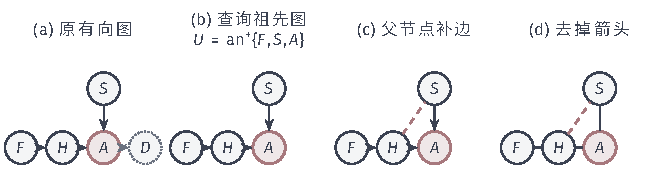
\includegraphics[width=156.951mm]{figures/06-probabilistic-graphical-models/01-representation/tikz/pgm-representations-ancestral-moralization/figure.pdf}
  \caption{报警查询的祖先道德图构造。原图以点线表示后代$D$及边$A\to D$。检验$F\perp S\mid A$时，祖先闭包为$U=\{F,H,A,S\}$，因此先去掉$D$及这条边。随后将$A$的父节点$H,S$相连，虚线表示新增的$H-S$边；再去掉原箭头，得到祖先道德图。红色的$A$是给定节点，检测分离时将其删除。}
  \label{fig:pgm-representations-ancestral-moralization}
\end{figure*}

图~\ref{fig:pgm-representations-ancestral-moralization}依次展示原有向图、查询祖先图、父节点补边和去箭头。点线标出随后筛除的后代，$H-S$虚线记录报警因子涉及的两个父节点。删除条件节点$A$后，路径$F-H-S$仍然连接，因此图不能推出$F\perp S\mid A$。若查询不包含$A$及其后代，祖先集合及由它产生的补边都可能不同。

\subsection{弦化与完美消元序}
\label{sec:pgm-representations-chordal-conversion}

推断时常常要逐个消去变量：第~\ref{chap:pgm-elimination}章会看到，消去$x_i$的标准做法是先把所有涉及$x_i$的局部因子相乘，再对$x_i$的各个状态求和。相乘后的新因子通常同时依赖$x_i$的若干个尚未删除的邻居；要让这个新作用域在无向图上仍是一个合法的团，这些邻居之间最好本来就有边。若它们缺边，就临时补一条边把作用域记录下来，这条边称为填充边；它也为无向表示改写成有向表示提供所需邻域结构。

图中不再有长度至少为四的诱导环时，就得到弦图。
给定节点顺序，本章将剩余邻域记为$N_k^+=\{v_\ell:\ell>k,\{v_k,v_\ell\}\in E\}$。
每个$N_k^+$中的剩余邻居都两两相连时，该顺序称为完美消元序；消元沿此顺序无需补边，边沿反序定向后，各节点的父节点也两两相连，形成完美有向图。

有限无向图存在完美消元序，当且仅当它是弦图。图~\ref{fig:pgm-representations-chordal-conversion}为四环加入$1-3$后，可按$(4,2,1,3)$消元：删除$4$或$2$时，剩余邻居$1,3$已由填充边相连；再删除$1$与$3$时，至多剩一个邻居，邻居两两相连的条件自动满足。将每条边从序中较晚的节点指向较早的节点，就得到无环且父集成团的有向图。定向采用消元次序的反序，因为当前节点的父节点正是尚未消去的邻居。

\begin{figure}[htbp]
  \centering
  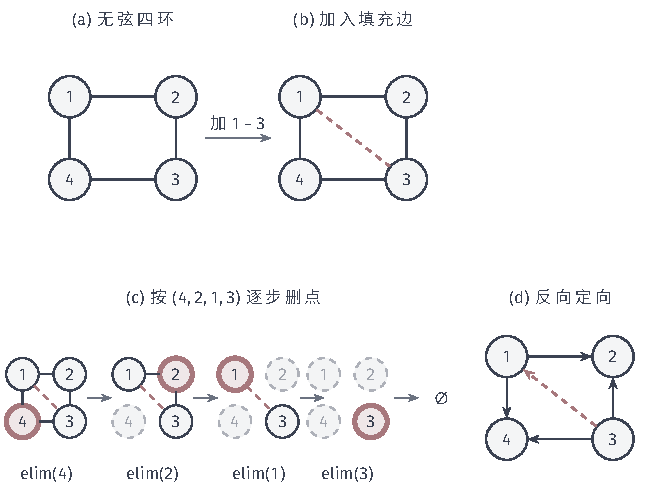
\includegraphics[width=112.000mm]{figures/06-probabilistic-graphical-models/01-representation/tikz/pgm-representations-chordal-conversion/figure.pdf}
  \caption{四环弦化及反序定向。加入虚线边$1-3$后，按完美消元序$(4,2,1,3)$删点；红色双圈为当前节点，灰色虚线轮廓为已删节点。各步下方的$\operatorname{elim}$标签记录被删除的节点，每一步的剩余邻居都两两相连。最后从序中较晚节点指向较早节点，实线箭头对应原四环的边，虚线箭头对应填充边。}
  \label{fig:pgm-representations-chordal-conversion}
\end{figure}

\Needspace{6\baselineskip}
\section{有向图与无向图的条件独立性关系}
\label{sec:pgm-representations-independence}

比较转换前后的独立性，需要精确描述两个集合：一个具体分布$p$实际满足的条件独立关系，以及一张图$\mathcal{G}$通过分离规则声明的条件独立关系。前者可能包含特殊参数造成的独立，后者则是结构对整类分布的保证。转换前后比较的，正是这两个集合之间的包含方向。下面先把它们写成集合，再定义三种刻画图与分布吻合程度的映射。

\subsection{独立性映射}
\label{sec:pgm-representations-maps}

将分布$p$的所有条件独立关系记为$\mathcal{I}(p)$：
\begin{equation}
  \mathcal{I}(p)
  =
  \bigl\{(A,B\mid S):
  \bm{X}_A\perp\bm{X}_B\mid\bm{X}_S\bigr\},
  \label{eq:pgm-representations-distribution-independences}
\end{equation}
查询集合$A,B,S\subseteq V$两两不交，$A,B$非空，条件集$S$允许为空。图的规则所蕴含的同类查询组成$\mathcal{I}(\mathcal{G})$：有向图按d-分离确定，无向图按无向分离确定。每项独立性按条件变量的分布成立；只在某个特殊条件值下成立的等式，未必属于这个集合。

这两个集合的包含方向决定图与分布的关系。图声明的独立越少，越不容易把本该相关的变量误判为独立；图声明的独立越多，对分布独立结构的限制越强。若图声明的关系全都属于分布的真实独立性，则称图为\term{独立性映射}（independency map, I-map）：图给出的每条独立保证都在分布中成立，但图可以只表达部分真实关系。若分布的全部独立性都能从图上读出，则称图为\term{依赖性映射}（dependency map, D-map）：图没有遗漏分布的任何独立，图上未被分离的变量在分布中也不独立。两个集合相等时，两项要求同时成立，图恰好刻画分布的全部独立结构，称为\term{完美映射}（perfect map）。

\begin{definition}[三类独立性映射]
  \label{def:pgm-representations-maps}
  对同一组随机变量的分布$p$与图$\mathcal{G}$，有
  \begin{equation}
    \begin{aligned}
      \mathcal{G}\text{是}p\text{的I-map}
      &\iff \mathcal{I}(\mathcal{G})\subseteq\mathcal{I}(p),\\
      \mathcal{G}\text{是}p\text{的D-map}
      &\iff \mathcal{I}(p)\subseteq\mathcal{I}(\mathcal{G}),\\
      \mathcal{G}\text{是}p\text{的完美映射}
      &\iff \mathcal{I}(\mathcal{G})=\mathcal{I}(p).
    \end{aligned}
    \label{eq:pgm-representations-map-inclusions}
  \end{equation}
\end{definition}

有向模型的可靠性保证$\mathcal{G}$是$p$的I-map；忠实性的反向蕴含再要求D-map方向成立，使有向图$\mathcal{G}$成为$p$的完美映射。这里的忠实性要求分布中的条件独立都能由图的d-分离解释，它用于排除特殊参数产生的额外独立性；其在关系识别中的作用可参考\BookChapterRef{chap:causal-inference}{卷2《数学准备：概率、因果与决策》中“因果响应”章}。

完全无向图与无边图提供了两个包含关系的极端。完全图没有分离任何两个非空节点集，因此没有独立性声明，对任意$p$都是I-map。无边图则声明所有互不相交的变量组在给定其他不交变量后独立，它的声明集包含任意$p$的真实关系，故总是D-map，通常却不是$p$的I-map。D-map的“依赖”可从逆否关系理解：对给定的$A,B,S$，图没有用$S$分离$A,B$时，$\bm{X}_A$与$\bm{X}_B$在$p$中给定$\bm{X}_S$也不独立。该保证覆盖全部查询。建模通常先满足I-map要求，因为任何错误的独立性约束都会将目标分布$p$排除在模型类之外\scite{pgm-koller2009}。

任何完全图都是I-map，但它一条独立都不声明，作为模型过于臃肿。建模时通常在保证I-map（不产生错误独立）的前提下尽量删边，因为边越少、因子越小、推断越省。若一张I-map的任一边被删后都会产生分布并不满足的错误声明，就称为\term{最小I-map}（minimal I-map）：再删任何一条边都会破坏安全性。这种最小性只针对当前图的单边删除，既不决定全体候选图中的最少边数，也不决定唯一图。例如两个二元变量取
\[
  p(0,0)=p(1,1)=0.4,\qquad
  p(0,1)=p(1,0)=0.1.
\]
两边缘都满足$p(X_1=0)=p(X_2=0)=0.5$，但$p(0,0)\ne0.25$，所以两变量依赖。$X_1\to X_2$与$X_1\leftarrow X_2$都没有额外独立声明；删边则会要求两变量独立，因此两图都是最小I-map。由此可见，单边删除的最小性保留了依赖，却无法确定方向。在一般图中，这种最小性还可能与遗漏其他真实独立性同时出现。

比较两张图时也可用同一包含方向：若$\mathcal{I}(\mathcal{G}_2)\subseteq\mathcal{I}(\mathcal{G}_1)$，称$\mathcal{G}_2$为$\mathcal{G}_1$的I-map。$\mathcal{G}_2$的独立性约束较少，仅受这些Markov约束、没有额外参数限制的分布族就较大。道德化与添加填充边通常给出这类较弱的独立性描述。

\subsection{d-分离的无向判据}
\label{sec:pgm-representations-ancestral-moralization}

第~\ref{sec:pgm-representations-ancestral-graphs}节构造的祖先道德图不只是示意，它恰好给出一个可操作的判据：d-分离不必再逐条路径分辨碰撞点，而可以完全转成无向图上的“删节点看连通”。选取查询祖先后，保留节点中的每个条件因子都只涉及这些节点；道德化再将其共同父节点相连。对所得无向图检查分离，可以精确回答原有向图的d-分离查询。

对有限DAG中两两不交的$A,B,S$，其中$A,B$非空，先取$U=\operatorname{an}^{+}(A\cup B\cup S)$，再在诱导图$\mathcal G[U]$上道德化。此时删去$S$后的无向分离，与原图中给定$S$的d-分离等价。这个等价关系只涉及图；后文将结合函数分解，证明分离查询所要求的概率独立性。

该判据在图上成立，因而与条件表参数及分布正性无关。检测按祖先闭包、诱导子图、道德化、删除条件节点$S$的次序进行：一个已观测的碰撞点在最后一步被删去，它的两个父节点之间的补边却应保留。先删除碰撞点会漏掉这条边，改变查询结果。Lauritzen的教材系统讨论祖先道德图与全局Markov性质\scite{pgm-lauritzen1996}。

对图~\ref{fig:pgm-representations-ancestral-moralization}中的$F\perp S\mid A$查询，最后删去$A$后，新增的$H-S$边仍留下路径$F-H-S$，所以当前图没有条件独立的保证。检验$F\perp S$时，祖先集合只有$\{F,S\}$，其余$H,A,D$都被去掉，剩余无边图给出独立性。同一原图的两个查询因此使用不同的祖先图，补边随$(A,B\mid S)$变化；未分离的查询仍可能在特殊参数下独立。

祖先闭包既保留端点，也保留导致间接联系的节点。例如$X_1\leftarrow X_0\to X_2$中，查询$X_1\perp X_2$需要$X_0$这个共同祖先；若仅留下$\{1,2\}$，两节点之间的联系会被误删。观测节点的祖先也有作用：在$X_1\to X_3\leftarrow X_2$、$X_3\to X_4$中，给定$X_4$激活了$X_3$处的碰撞点。查询$\{1\}$与$\{2\}$给定$\{4\}$时，祖先图保留$X_3$，随后道德化生成$1-2$边，记录这条被激活的联系。

若改为一次性道德化整个报警模型，新增边在所有查询中都保留。即使没有给定$A$，路径$F-H-S$也存在，原来的$F\perp S$就无法从整张道德图读出。\emph{整个有向图的道德图}用于重组联合函数的全部作用域，\emph{为查询构造的祖先道德图}则用于精确回答某项分离；整体图通常声明的独立性更少，其关系为
\begin{equation}
  \mathcal{I}\bigl(\operatorname{mor}(\mathcal{G})\bigr)
  \subseteq \mathcal{I}(\mathcal{G}),
  \label{eq:pgm-representations-moral-inclusion}
\end{equation}
整体图中被$S$分离的两侧，在较小的查询祖先道德图中仍被分离，所以整体图能证明部分d-分离。整体图中连通时，查询祖先图却可能已删除造成连通的节点或补边，因此原有向图仍可能满足这项d-分离。

\subsection{有向图独立性结论的证明}
\label{sec:pgm-representations-directed-proofs}

本节集中补全第~\ref{chap:pgm-directed}章引用但未展开的几个证明，第一次阅读时若主要关心结论与转换方法，也可以先跳过本节、直接进入第~\ref{sec:pgm-representations-factorizations}节的因子分解比较。证明的主线是：先用祖先道德图让局部因子的作用域全部落成团，从而把第~\ref{chap:pgm-undirected}章“分离后两侧分别归一化”的技巧搬到有向图上；再据此依次证明d-分离的可靠性、有向Markov毯以及模型类完备性。下面先说明局部条件分布如何归一化并产生联合分解，作为后续证明的共同基础。

\begin{proof}[引理~\ref{lem:pgm-directed-normalization}的证明]
取拓扑序中最后的节点，它没有子节点，只出现在自己的局部条件因子内。对其取值关于$\mu_i$积分，该因子由局部归一化变成$1$。继续逆拓扑序消去剩余节点，非负性允许用Tonelli定理交换积分次序，最后整个乘积的积分为$1$。有限离散状态下，同一操作就是逐节点求和。

求祖先集合的边缘分布时，仅需消去$V\setminus W$。集合$W$包含各节点的全部祖先，故$V\setminus W$中的节点没有位于$W$的子节点。逆拓扑序处理补集时，当前节点在补集中的子节点也已被消去，所以它仍只出现在自己的因子中。每次积分都将此因子变为一，最终留下式~\eqref{eq:pgm-directed-ancestral-marginal}中祖先节点的因子。
\end{proof}

\begin{proof}[定理~\ref{thm:pgm-directed-ordered-factor}的证明]
使用有序Markov假设指定的拓扑序，将联合概率按链式法则展开：
\[
  p(x_1,\ldots,x_d)=
  \prod_{i=1}^{d}p(x_i\mid x_1,\ldots,x_{i-1}).
\]
父节点都在当前节点之前。式~\eqref{eq:pgm-directed-ordered}使每个节点的条件分布只需保留前驱中的父节点变量：
\[
  p(x_i\mid\bm{x}_{\operatorname{pre}(i)})
    =p(x_i\mid\bm{x}_{\operatorname{pa}(i)}).
\]
代回链式法则，就得到式~\eqref{eq:pgm-directed-factorization}的父子分解。条件等式按前驱配置的分布几乎处处成立，因此还需说明零概率配置不会破坏乘积相等。

在有限离散情形，将按父配置选定的条件表记为$q_i$。父配置具有正概率时，$q_i$就是原分布的相应条件概率；父配置概率为零时，才可任选一行归一化概率来补全。完整前驱配置为零，未必意味着它包含的父配置也为零，所以不能据此前缀任意改变一行已经确定的父条件表。链式条件分布在零概率前驱上的版本可任意选择，与父条件表的补全范围需要分开。

记原分布前$k$个变量的边缘质量函数为$p_k$，并定义局部乘积
\[
  \widehat p_k(x_1,\ldots,x_k)
    =\prod_{i=1}^k q_i(x_i\mid\bm{x}_{\operatorname{pa}(i)}),
  \qquad \widehat p_0=p_0=1.
\]
我们按前缀长度证明$\widehat p_k=p_k$。若某个前缀满足$p_k(x_1,\ldots,x_k)>0$，下一节点的父配置也有正概率。有序Markov性质便将该前缀下的链式条件概率约简为已选定的$q_{k+1}$，因而
\[
  \begin{aligned}
    \widehat p_{k+1}
      &=\widehat p_k\,q_{k+1}
       =p_k\,p(x_{k+1}\mid x_1,\ldots,x_k)\\
      &=p_{k+1}.
  \end{aligned}
\]
若旧前缀的概率为零，归纳假设给出$\widehat p_k=0$，乘上下一张合法条件表后仍为零；原分布中任一延长前缀的概率也不超过旧前缀概率，所以$p_{k+1}=0$。这一步不改变正概率父配置上的条件表，也允许在零概率父配置上采用先前任意补全的行。两种情况覆盖全部前缀，从而在$k=d$得到所需联合分解。

连续密度则使用相应条件版本和积分的链式法则，得到几乎处处相同的联合密度。某个点的密度为零并不等同于离散前缀事件的概率为零，所以上面的逐配置归纳只用于有限离散情形。这一展开及约简都沿最初指定的同一拓扑序进行。
\end{proof}

\begin{proof}[定理~\ref{thm:pgm-directed-factor-local}的证明]
固定节点$i$，取非后代集合$N=\operatorname{nd}(i)$。其中各节点的祖先都仍在$N$中：若祖先是$i$或其后代，该节点就会成为$i$的后代；而$i$本身的祖先也在$N$内。因此，$N$与$N\cup\{i\}$都是祖先闭合集合，可以用引理~\ref{lem:pgm-directed-normalization}边缘化：
\[
  \begin{aligned}
    p(x_i,\bm{x}_N)
      &=q_i(x_i\mid\bm{x}_{\operatorname{pa}(i)})
        \prod_{j\in N}q_j(x_j\mid\bm{x}_{\operatorname{pa}(j)})\\
      &=q_i(x_i\mid\bm{x}_{\operatorname{pa}(i)})p(\bm{x}_N).
  \end{aligned}
\]
在有效条件值上约去非后代的边缘分布，得到$p(x_i\mid\bm{x}_N)=q_i(x_i\mid\bm{x}_{\operatorname{pa}(i)})$。再消去$N\setminus\operatorname{pa}(i)$，可见$q_i$也给出$p(x_i\mid\bm{x}_{\operatorname{pa}(i)})$的一个版本。给定父节点后，其他非后代不再改变节点的条件分布，局部Markov性质因而成立。

任一固定拓扑序都满足$\operatorname{pre}(i)\subseteq N$。在刚得到的局部独立关系中消去其余非后代，就获得该顺序下的有序Markov性质。由此，一个父子分解先推出局部性质，再推出所有拓扑序的有序性质。
\end{proof}

全局证明将查询祖先图内的因子分为两组。下面以离散求和书写；连续变量具有联合密度时，使用相应基准测度的积分，非负性使Tonelli定理适用。

\begin{proof}[定理~\ref{thm:pgm-directed-soundness}的证明]
取$p\in\mathcal{M}(\mathcal{G})$，并设查询满足$A\perp_{\mathcal{G}}B\mid S$。定理~\ref{thm:pgm-directed-ordered-factor}将$p$写成$\mathcal{G}$上的条件因子乘积，以$q_i(x_i\mid\bm{x}_{\operatorname{pa}(i)})$记节点$i$的因子。取查询祖先集合$R=\operatorname{an}^{+}(A\cup B\cup S)$，由引理~\ref{lem:pgm-directed-normalization}消去$V\setminus R$，留下
\[
  p(\bm{x}_R)=
  \prod_{i\in R}q_i(x_i\mid\bm{x}_{\operatorname{pa}(i)}).
\]
每个因子的作用域$\{i\}\cup\operatorname{pa}(i)$都在$\operatorname{mor}(\mathcal{G}[R])$中构成团。因此，删去$S$后，同一个因子剩余的节点都在同一连通分量中；两两相连的节点无法分属不同分量。

在$\operatorname{mor}(\mathcal{G}[R])\setminus S$中，将与$A$相交的分量合为$C$，其他节点合为$D=R\setminus(C\cup S)$。祖先道德化判据保证$B\subseteq D$。将涉及$C$的因子相乘记为$g(\bm{x}_C,\bm{x}_S)$，涉及$D$的因子相乘记为$h(\bm{x}_D,\bm{x}_S)$，其余只涉及$S$的因子相乘记为$k(\bm{x}_S)$，得到
\[
  p(\bm{x}_R)=
  g(\bm{x}_C,\bm{x}_S)
  h(\bm{x}_D,\bm{x}_S)
  k(\bm{x}_S).
\]
将未查询的$C\setminus A$和$D\setminus B$变量分别从两侧消去，所得函数记为$g_A,h_B$。乘积因此仍分为查询的两侧：
\[
  p(\bm{x}_A,\bm{x}_B,\bm{x}_S)=
  g_A(\bm{x}_A,\bm{x}_S)
  h_B(\bm{x}_B,\bm{x}_S)
  k(\bm{x}_S).
\]
固定具有正且有限边缘质量或密度的$\bm{x}_S$，将两侧总权重分别记为$G(\bm{x}_S)=\sum_{\bm{x}_A}g_A(\bm{x}_A,\bm{x}_S)$和$H(\bm{x}_S)=\sum_{\bm{x}_B}h_B(\bm{x}_B,\bm{x}_S)$。归一化条件联合分布时，这两个常数各自归一化一侧函数：
\[
  \begin{aligned}
    p(\bm{x}_A,\bm{x}_B\mid\bm{x}_S)
      &=\frac{g_A(\bm{x}_A,\bm{x}_S)}{G(\bm{x}_S)}
        \frac{h_B(\bm{x}_B,\bm{x}_S)}{H(\bm{x}_S)}\\
      &=p(\bm{x}_A\mid\bm{x}_S)
        p(\bm{x}_B\mid\bm{x}_S).
  \end{aligned}
\]
上述比值使用正概率条件事件或几乎处处的有效条件密度。两侧条件边缘相乘，便得到目标条件独立性。函数可以在部分联合配置取零，这个证明仍然成立。
\end{proof}

\begin{proof}[定理~\ref{thm:pgm-directed-markov-blanket}的证明]
以$O=V\setminus(\{i\}\cup\operatorname{mb}(i))$表示毯外节点。$O=\varnothing$时，独立侧为空，结论平凡成立。取$O\neq\varnothing$，考察从$i$到$O$中任一节点的路径。它的首步必经父节点或子节点，两类节点都在$\operatorname{mb}(i)$中。

首步经过父节点$j\to i$时，$j$在路径上有一个箭尾，是非碰撞点；它又满足$j\in\operatorname{mb}(i)$，所以被观测后阻断路径。首步经$i\to j$再沿$j\to k$离开时，子节点$j$同样是已观测的非碰撞点。若路径以$i\to j\leftarrow k$开始，$j$是已观测的碰撞点，但$k$是子节点的另一个父节点，也在$\operatorname{mb}(i)$内。此时$k$仍不是路径终点，且$k\to j$的箭尾使它成为已观测的非碰撞点，路径转而在这里被阻断。

三种首段覆盖了从$i$到$O$的所有路径，每条都被$\operatorname{mb}(i)$阻断，故$i\perp_{\mathcal G}O\mid\operatorname{mb}(i)$。应用定理~\ref{thm:pgm-directed-soundness}的可靠性，得到节点与毯外变量的条件独立。

在有效条件分布上，局部函数也给出同一屏蔽关系。按定理~\ref{thm:pgm-directed-ordered-factor}分解联合概率，给定其余变量后，只有节点$i$及其子节点的因子仍含$x_i$：
\begin{equation}
  \begin{aligned}
    p(x_i\mid\bm{x}_{V\setminus\{i\}})
      &\propto q_i(x_i\mid\bm{x}_{\operatorname{pa}(i)})\\
      &\quad{}\times
      \prod_{j\in\operatorname{ch}(i)}
        q_j(x_j\mid\bm{x}_{\operatorname{pa}(j)}).
  \end{aligned}
  \label{eq:pgm-directed-blanket-conditional}
\end{equation}
右侧的其他自变量全在$\operatorname{mb}(i)$中，因而对$x_i$归一化后，条件分布仍只使用毯内变量。这里的比例式用于条件分布有定义的配置；零概率条件配置采用第~\ref{chap:pgm-directed}章说明的条件分布版本。
\end{proof}

上述结果连起了第~\ref{chap:pgm-directed}章的四种表述：定理~\ref{thm:pgm-directed-ordered-factor}由有序Markov性质得到因子分解，定理~\ref{thm:pgm-directed-soundness}再由分解得到全局性质，引理~\ref{lem:pgm-representations-global-to-local}由全局得到局部，最后定理~\ref{thm:pgm-directed-factor-local}的边缘化论证由局部得到任一拓扑序的有序性质。于是式~\eqref{eq:pgm-directed-equivalence}的等价关系成立；各步都允许联合分布在某些配置取零。

可靠性只回答了“被d-分离的一定独立”，完备性还要回答相反的一面：没有被d-分离的查询，模型类中是否真的存在一个分布让两端相关？若不存在，d-分离规则就漏报了某些结构强制的独立。完备性证明通过构造“依赖见证”分布完成。最简单的连续情形只含一个碰撞点（或其后代被观测），可用高斯条件协方差直接算出非零依赖；一般图含多个碰撞点、多条路径时，不同路径的数值作用可能相互抵消，需要随后的非平凡性引理统一处理。对于图$X\to Z\leftarrow Y$及$Z\to D$，定义
\[
  \begin{aligned}
    X&=\varepsilon_X,& Y&=\varepsilon_Y,\\
    Z&=X+Y+\varepsilon_Z,& D&=Z+\varepsilon_D,
  \end{aligned}
\]
四个噪声相互独立，均取$\mathcal{N}(0,1)$分布。独立根节点使$X,Y$边缘独立，整个系统满足上述有向分解。噪声方差相加得到$\operatorname{Var}(Z)=3$，而$D=Z+\varepsilon_D$再增加一项独立噪声，所以$\operatorname{Var}(D)=4$。两个根变量与$Z$的协方差均为$1$；与$D$的协方差也均为$1$，因为新增噪声与根变量独立。观测碰撞点或其后代后，可用这些量和高斯条件协方差公式直接计算两根节点的关系：
\[
  \begin{aligned}
    \operatorname{Cov}(X,Y\mid Z)
      &=0-\frac{1\cdot1}{3}=-\frac13,\\
    \operatorname{Cov}(X,Y\mid D)
      &=0-\frac{1\cdot1}{4}=-\frac14.
  \end{aligned}
\]
条件协方差可由回归残差得到：分别将两个根变量对观测作线性回归，再计算残差的协方差。例如观测$Z$时，两个回归系数均为$1/3$，残差为$X-Z/3$与$Y-Z/3$，其协方差是$0-1/3-1/3+3/9=-1/3$；观测$D$时同理将系数换为$1/4$。联合高斯的残差与观测独立，因而该值就是条件协方差。上面两个非零结果分别给出观测碰撞点及其后代后的依赖；要覆盖一般有向图的所有活跃路径，还需要下一步的非平凡性结果。

一般图的活跃路径可含多个碰撞点，通向条件节点的路径也可能交会。不同路径的数值作用可能抵消，因此非零边系数本身不足以提供依赖见证。图~\ref{fig:pgm-directed-cancellation}展示一个明确的抵消参数：
\[
  X=\varepsilon_X,\qquad
  Z=X+\varepsilon_Z,\qquad
  Y=-X+Z+\varepsilon_Y,
\]
噪声仍相互独立且服从$\mathcal N(0,1)$。代入中间变量后得到$Y=\varepsilon_Z+\varepsilon_Y$，故$X\perp Y$：三个边系数虽然非零，直接与间接路径上的作用却恰好相消。若将$X\to Y$的系数改为$-1+\delta$，就有$\operatorname{Cov}(X,Y)=\delta$。当$\delta\ne0$时，这项额外独立性消失。

\begin{figure}[htbp]
  \centering
  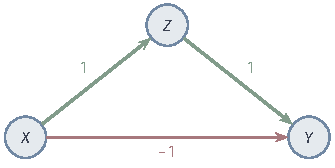
\includegraphics[width=56.653mm]{figures/06-probabilistic-graphical-models/01-representation/tikz/pgm-directed-cancellation/figure.pdf}
  \caption{直接与间接作用相消的高斯模型。$X\to Y$的系数为$-1$，经$Z$的两个系数均为$1$，代入后两项相消。两条路径对空条件集都活跃，这组参数却使$X$与$Y$独立。}
  \label{fig:pgm-directed-cancellation}
\end{figure}

完备性需要证明，对每项活跃查询，其条件独立约束并未在整个相容参数空间中恒成立。为检验这一点，先将条件独立写为一个等式，再将等式改写成模型参数的多项式取零。这样，图上的依赖见证问题就转成了参数空间中能否找到违反该等式的点。

高斯情形可以沿用刚才的条件协方差判据。记全体变量的协方差矩阵为$\bm\Sigma$；在非退化联合高斯模型中，两个标量条件独立，等价于它们的条件协方差为零。计算这个条件协方差需要对条件变量的协方差块$\bm\Sigma_{S,S}$求逆；乘以正的$\det(\bm\Sigma_{S,S})$后，可将逆矩阵带来的分母消去。所得量正是行指标为$(u,S)$、列指标为$(v,S)$的交叉子式，后面的分块行列式计算会给出这一关系。因此，这个子式取零等价于对应的标量条件协方差取零。

离散情形在$p(\bm x_S)>0$的配置上，将条件独立等式两侧的条件概率换成联合概率比值，再交叉相乘，得到下面的两项概率乘积之差。若$p(\bm x_S)=0$，相关联合质量也都为零，交乘式自动成立，无需在零概率事件上取比值。联合概率是有限个条件表项的乘积，边缘概率又是联合概率的有限和，所以该差也是条件表自由参数的多项式。

这里的“非零多项式”表示它不恒等于零，允许在特殊参数处取零；抵消例正是这样的特殊取值。下面的引理将活跃路径的图论条件转为多项式不恒为零的保证，之后的代数步骤由此选择一个违反独立约束的参数。离散结论及路径构造采用Meek的强完备性结果，高斯结论采用线性高斯有向图的多项式完备性结果\scite{pgm-directed-meek1995,pgm-koller2009}。

\begin{lemma}[条件独立约束的非平凡性]
  \label{lem:pgm-directed-nontrivial}
  设$\mathcal{G}=(V,E)$为有限有向无环图，$u,v\in V$为不同节点，$S\subseteq V\setminus\{u,v\}$，且$u,v$在$\mathcal{G}$中给定$S$时d-连接，则以下两项成立。
  \begin{enumerate}
    \item 对$i\in V$，在线性高斯系统
    \[
      X_i=\sum_{j\in\operatorname{pa}(i)}b_{i,j}X_j+\varepsilon_i,
      \qquad
      \varepsilon_1,\ldots,\varepsilon_d
      \mathrel{\overset{\mathrm{ind}}{\sim}}\mathcal N(0,1)
    \]
    中，记边系数为$\bm{\theta}$、协方差矩阵为$\bm{\Sigma}(\bm{\theta})$，则
    \[
      f_{u,v,S}(\bm{\theta})
      =\det\bm{\Sigma}_{(u,S),(v,S)}(\bm{\theta})
    \]
    是非零多项式。行指标按$u$及$S$排列，列指标按$v$及同一顺序的$S$排列；$S=\varnothing$时，该式为$\Sigma_{u,v}$。
    \item 固定每个节点至少含两个状态的有限状态空间，并用各行前$r_i-1$个概率参数化局部条件表。将联合概率与边缘概率写成这些参数的多项式后，在所有状态配置对应的条件独立多项式
    \[
      p(x_u,x_v,\bm{x}_S)p(\bm{x}_S)
      -p(x_u,\bm{x}_S)p(x_v,\bm{x}_S)
    \]
    中，至少有一个不是零多项式。
  \end{enumerate}
\end{lemma}

本章采用这一外部引理，下面的证明以它为前提。引理所处理的是活跃路径及碰撞点通向$S$的有向路径：从中提取保留连接的子图，并控制路径交会时的代数抵消。高斯模型可以使用任意正噪声方差，这里的单位方差子类已足够构造所需见证；逐坐标可逆缩放也保持条件独立性。具体地，若原噪声标准差为$\sigma_i>0$，令$Y_i=X_i/\sigma_i$，新噪声就具有单位方差，边系数则变为$b_{i,j}\sigma_j/\sigma_i$。这种缩放没有丢掉任何坐标信息，所以不会改变条件独立关系。

\begin{proof}[定理~\ref{thm:pgm-directed-completeness}的线性高斯部分]
集合$A,B$未被$S$ d-分离时，可选由活跃路径连接的$u\in A,v\in B$。将引理~\ref{lem:pgm-directed-nontrivial}的线性系统按拓扑序写为矩阵形式，得到$\bm X=\bm B\bm X+\bm\varepsilon$；系数矩阵$\bm{B}$严格下三角，非边元素为零。于是$\bm X=(\bm I-\bm B)^{-1}\bm\varepsilon$，再利用$\bm{B}^d=\bm 0$，得到
\[
  \begin{aligned}
    \bm{L}&=(\bm{I}-\bm{B})^{-1}
       =\bm{I}+\bm{B}+\cdots+\bm{B}^{d-1},\\
    \bm{\Sigma}(\bm{\theta})&=\bm{L}\bm{L}^{\top}.
  \end{aligned}
\]
有限矩阵和使协方差各元素都成为边系数的多项式；对任意实边系数，可逆的线性变换又保证$\bm{\Sigma}$正定。将条件协方差写入分块行列式，可得
\[
  f_{u,v,S}(\bm{\theta})
    =\det(\bm{\Sigma}_{S,S})
      \bigl(\Sigma_{u,v}
        -\bm{\Sigma}_{u,S}\bm{\Sigma}_{S,S}^{-1}
         \bm{\Sigma}_{S,v}\bigr).
\]
括号给出$\operatorname{Cov}(X_u,X_v\mid\bm X_S)$。$S$为空时，空矩阵行列式取$1$，矩阵求逆项无需执行。高斯条件分布的两个标量独立当且仅当这个协方差为零。引理保证$f_{u,v,S}$为非零多项式，所以可以选取使条件协方差非零的系数。

存在性还可落实为有限终止的枚举：逐渐增大有理数分子绝对值及正分母的上界，枚举有理边系数向量，用有理数运算计算行列式，找到非零值即停止。非零多项式在某个实参数点附近仍非零，有理向量的稠密性保证枚举能进入这个邻域。输出系数与单位独立高斯噪声定义了$\mathcal{M}_{\mathrm{LG}}(\mathcal{G})$中的分布，满足$X_u\not\perp X_v\mid\bm X_S$。若向量$\bm X_A,\bm X_B$条件独立，每对分量也应条件独立，因而与上述结果矛盾。这给出了查询的见证构造，但并未给出高效寻找见证的算法。
\end{proof}

有限离散模型改用条件表参数。每一行取前若干状态概率为自由参数，末状态概率由行和为$1$确定。各自由坐标大于$0$且每行自由坐标之和小于$1$，恰好保证整行严格为正。这些都是严格不等式，多行参数的笛卡尔积因而在有限维参数空间中形成开集；每行均匀分布给出其中一个点，说明该开集非空。联合概率与边缘概率都是这些参数的多项式。严格正性保证$p(\bm x_S)>0$，所以给定$S$时$X_u$与$X_v$条件独立，等价于每种状态配置都满足
\[
  \begin{aligned}
    &p(x_u,x_v,\bm x_S)p(\bm x_S)\\
    &\qquad{}-p(x_u,\bm x_S)p(x_v,\bm x_S)=0.
  \end{aligned}
\]

要从不恒为零走到这个严格正参数域内的见证，还需知道：非零多项式的零点不可能占满一个非空开集。下面用零点集的测度说明这一事实，也为随后同时避开多项额外独立约束作准备。

\begin{lemma}[非零多项式的零点集]
  \label{lem:pgm-representations-polynomial-zero-set}
  设$f$是$\mathbb R^m$上不恒为零的实多项式，$m\geq1$。其零点集具有$m$维Lebesgue测度零，因此不能包含非空开集。
\end{lemma}

\begin{proof}
记$\lambda_m$为$m$维Lebesgue测度。$m=1$时，非零多项式只有有限个实根，故零点集的测度为零。设结论对$m-1$个变量成立，将$m$元多项式按最后一个坐标$t$展开为
\[
  f(\bm y,t)=\sum_{\ell=0}^{K}a_\ell(\bm y)t^\ell,
  \qquad \bm y\in\mathbb R^{m-1}.
\]
至少有一个系数多项式$a_{\ell_0}$不恒为零。使所有系数同时为零的底点集合记为$E$，它包含在$a_{\ell_0}$的零点集中，因归纳假设而有$\lambda_{m-1}(E)=0$。在$E$之外，每个固定$\bm y$对应一元非零多项式，它的零点只有有限个，故沿$t$方向的截面测度为零。

先将零点集限制在盒$[-M,M]^m$内，其中$M$为正整数。在坏底点$E$上，截面长度至多为$2M$；在其余底点上，截面长度为零。零点集是闭集，可以对其非负指标函数使用Tonelli定理，按底点与最后一个坐标分别积分。积分只可能在零测的$E$上贡献至多$2M$，所以整个盒内零点集的$m$维测度仍为零。再令$M=1,2,\ldots$，这些盒覆盖全空间，可数个零测集的并仍为零测集。任一非空开集含有边长为正的小盒，具有正测度，因此不能包含在该零点集中。
\end{proof}

\begin{proof}[定理~\ref{thm:pgm-directed-completeness}的有限离散部分]
取活跃路径连接的$u\in A,v\in B$。引理~\ref{lem:pgm-directed-nontrivial}的第二项保证，有限组条件独立多项式中至少一项非零。由引理~\ref{lem:pgm-representations-polynomial-zero-set}，非零多项式在参数空间的非空开集上无法恒为零。严格正条件表参数域正是这样的开集，所以其中必有一点使选定多项式非零，至少一个独立等式随之失败。所得联合分布属于$\mathcal{M}_{\mathrm{disc}}^{+}(\mathcal{G})$，并满足$X_u\not\perp X_v\mid\bm X_S$。向量$\bm X_A\perp\bm X_B\mid\bm X_S$若成立，会推出所有坐标对条件独立，与选定坐标对的结论矛盾。故$\bm X_A\not\perp\bm X_B\mid\bm X_S$，有限离散类也存在所需见证。
\end{proof}

对固定有限图，所有节点对及条件集合的查询只有有限多组。为每项未分离查询选定一个非零检验多项式：高斯情形选上述交叉子式，离散情形选引理保证不恒为零的某一状态配置等式。该查询若出现额外独立性，选定多项式就必须取零。因此，导致该查询额外独立的坏参数集包含在一个零测集中，而不要求它恰好等于整个零点集。有限个这样的零点集之并仍为零测集，无法覆盖具有非空内部的合法参数域。选取并集之外的同一组参数，就能同时避免所有节点对查询的额外独立性；任何未分离的向量查询又含有一对活跃连接的坐标，故也不可能额外独立。

这一论证也覆盖正噪声方差自由变化的线性高斯模型，而不限于构造见证所用的单位方差子类。令$\tau_i>0$为第$i$项噪声方差，协方差变为$\bm\Sigma=\bm L\operatorname{diag}(\tau_1,\ldots,\tau_d)\bm L^\top$，其元素仍是边系数和方差坐标的多项式。每个检验多项式在所有$\tau_i=1$的子类中已不恒为零，所以在更大的参数空间中也不恒为零；正方差条件给出的域仍是非空开集。截距只改变均值，不影响这些条件独立判据，把截距也列作自由坐标后仍可使用同一零点集结论。因此，在上述没有额外约束的离散或线性高斯参数族中，忠实分布存在，不忠实参数组成零测集。真实系统可能具有特殊参数；接近抵消集合时，依赖还可能很弱，使有限样本难以分辨。

\subsection{两类独立性表示的差异}
\label{sec:pgm-representations-independence-differences}

查询祖先道德图随端点和条件集合而变化；一张固定的无向图未必能同时复现所有d-分离。例如碰撞结构$X_1\to X_3\leftarrow X_2$声明$X_1\perp X_2$，没有声明$X_1\perp X_2\mid X_3$。无向图若使$1$与$2$被空集分离，两节点之间原本就无路径；再删$3$仍然分离。这个单调性与碰撞查询的变化冲突，所以同一节点集合上无法找到完全相同的无向分离集合。特殊参数产生的分布仍可由两类图共同表示，当前反例比较的是图的全部独立性声明。

从无向图转向有向图也存在表达边界。图~\ref{fig:pgm-representations-chordal-conversion}左侧四环$1-2-3-4-1$没有对角边$1-3$或$2-4$，同时声明
\begin{equation}
  X_1\perp X_3\mid(X_2,X_4),\qquad
  X_2\perp X_4\mid(X_1,X_3).
  \label{eq:pgm-representations-cycle-independences}
\end{equation}
给这个骨架作无环定向，至少一个节点会同时接收两条环边。例如$2\to1\leftarrow4$的两父节点$2$与$4$不相邻，形成未遮蔽碰撞点。给定$\{1,3\}$会打开路径$2\to1\leftarrow4$，所以d-分离无法得到式~\eqref{eq:pgm-representations-cycle-independences}的第二项。

这一碰撞点可由拓扑序直接找出：四环中排在最后的节点，其两个邻居都在前，故两条边都指向它。更换拓扑序会改变碰撞的位置，仍会留下一个未遮蔽碰撞点。

改变骨架也无法保留原来的全部独立性。对有向图中两个不相邻节点$i,j$，无环性保证可以选一个节点，例如$i$，使$j$是它的非后代。$j$又不是$i$的父节点，第~\ref{chap:pgm-directed}章证明局部Markov性质时所用的图分离关系便给出$i\perp_{\mathcal G}j\mid\operatorname{pa}(i)$。这一步只涉及图；再应用可靠性，才得到相容分布中的$X_i\perp X_j\mid\bm{X}_{\operatorname{pa}(i)}$。无向图中的非邻接对则被其余全部节点分离。相邻对在两类图中都保留长度为一的路径，任何不含端点的条件集都无法阻断它。由此，全部图分离关系能确定邻接关系，两张图独立性集合相同时也必有同一骨架。

碰撞结构的观测激活与四环的两项对角条件独立，分别超出了另一类图在同一节点集上的完美表示范围，所以两类图的独立性表达能力一般互不包含。第~\ref{sec:pgm-representations-chordal-conversion}节的弦图和完美有向图则提供了可相互保留全部分离关系的结构条件。

\subsection{完美表示的条件}
\label{sec:pgm-representations-perfect-dags}

碰撞结构和无弦四环说明两类图的独立性表达能力一般互不包含。能够无损保留全部分离关系的结构由弦图以及“父集成团”的有向图给出，二者是同一性质在两种图上的体现。以下两个判定分别用于无向到有向、有向到无向的完美表示。

对于有限无向图，要在同一节点集合上用DAG保留全部分离关系，原图必须是弦图，而弦图也允许这种改写。选取一个完美消元序，将每条边从序中较晚的节点指向较早的节点，便得到所需的完美有向图。此时原剩余邻域成为父集，每个父集中的节点两两相连。


对有限DAG，同一节点集合上的完美无向表示，要求各节点父集内的节点两两相连；这个条件也足以保证表示存在。每个父集内的节点已经两两相连时，道德化无需额外补父节点之间的边，去掉方向后的骨架就是弦图，并保留同样的分离关系。

“完美有向图”的判定只用父集是否成团；“$\mathcal{D}$是$p$的完美映射”则比较图与某个分布的独立性。即使$\mathcal{D}$和$\mathcal{U}$的分离集合完全相等，特殊参数仍可能让$p$具有额外独立性。这两种转换保证的是图之间的完美表示，具体分布的完美映射还需忠实性。

原图不满足弦性时，可以添加边后再定向。图~\ref{fig:pgm-representations-chordal-conversion}为四环补$1-3$，产生极大团$\{1,2,3\}$与$\{1,3,4\}$。以$\mathcal{U}$记原图、$\widetilde{\mathcal{U}}$记弦化图，则有
\[
  \mathcal{I}(\widetilde{\mathcal{U}})
  \subseteq \mathcal{I}(\mathcal{U}).
\]
填充边增加可用路径，因而新分离集合只能缩小。四环的$X_2\perp X_4\mid(X_1,X_3)$仍能从新图读出，$X_1\perp X_3\mid(X_2,X_4)$却因为新增对角边而失去图上的保证。弦化换来了所需的消元和定向结构，也可能减少可见的独立性。

\section{有向图与无向图的因子分解关系}
\label{sec:pgm-representations-factorizations}

前两节从结构和独立性两个层面比较了两种图，本节转向第三个层面：局部函数怎样重组，才能在换图的同时保持联合分布的每一个概率值都不变。以下固定一个给定分布$p$，说明它的条件分布与团势如何互相改写，同时区分“对这一个分布的精确改写”与“转换后那张图所允许的整类自由参数模型”。后者通常比原来的分布族更大，因为一旦不再约束新表项之间的关系，模型就能表达转换前没有的分布。两种分解在归一化方式上的差异，决定了转换时必须额外处理的内容。

\subsection{两类因子分解的差异}
\label{sec:pgm-representations-normalization}

有向图把联合分布写成每个节点给定父节点的条件分布乘积：
\begin{equation}
  p(\bm{x})=\prod_{i\in V}
  p(x_i\mid\bm{x}_{\operatorname{pa}(i)}).
  \label{eq:pgm-representations-directed-product}
\end{equation}
每个父配置下，局部条件表都满足$\sum_{x_i}p(x_i\mid\bm{x}_{\operatorname{pa}(i)})=1$。从没有子节点的节点开始求和，它只在自己的条件因子中出现，这个因子因此变成$1$。剩余图仍无环，可以继续同样的操作，最后得到$\sum_{\bm{x}}p(\bm{x})=1$。局部归一化与无环结构共同保证了联合归一化。

Markov网络使用团上的非负势，另以全局配分函数归一化：
\begin{equation}
  p(\bm{x})=\frac{1}{Z}
  \prod_{C\in\mathcal{C}}\psi_C(\bm{x}_C),
  \qquad
  Z=\sum_{\bm{x}}\prod_{C\in\mathcal{C}}\psi_C(\bm{x}_C),
  \label{eq:pgm-representations-undirected-product}
\end{equation}
所选团作用域组成$\mathcal{C}$，其中可含极大团或较小团，且需满足$0<Z<\infty$。势表给出相对权重，对单个变量的求和可以异于$1$。不同势共享坐标，逐表归一化后，整体乘积仍需自己的归一化常数。将一个势乘以正常数时，$Z$同比缩放，分布$p$保持原样；这种尺度自由度构成势参数的冗余。

连续变量改用指定乘积测度的积分，函数需可测、非负且可归一化，局部密度也以积分为一理解。已给定非负团分解时，全局Markov性质允许零配置；从独立性反推团分解，则采用上一章说明的严格正性等条件。下面的条件表重组使用有限离散严格正分布，使每步条件归一化的分母都为正。

\subsection{从有向因子分解到无向因子分解}
\label{sec:pgm-representations-directed-to-undirected}

从有向因子分解转换到无向因子分解更直接。有向条件因子$p(x_i\mid\bm{x}_{\operatorname{pa}(i)})$虽然带有“$i$条件于父节点”的方向含义，但作为普通多变量函数，它只依赖$\{i\}\cup\operatorname{pa}(i)$这一组变量，见式~\eqref{eq:pgm-representations-directed-product}。只要在无向图中把这个“家庭集合”连成一个团，就可以直接把整张条件表当成该团上的势，函数值保持不变。整体道德化恰好完成补边，使每个家庭集合都成为团，因此原条件分布可作为该团的势：
\[
  \psi_{\{i\}\cup\operatorname{pa}(i)}
  (x_i,\bm{x}_{\operatorname{pa}(i)})
  =
  p(x_i\mid\bm{x}_{\operatorname{pa}(i)}),
\]
全部势相乘仍是原来的条件分布乘积；相同作用域的因子可以保留，也可以合并。原联合分布已归一化，故此时$Z=1$。若只保留极大团势，就给每个因子选择一个包含它的极大团，在团内相乘；未接收因子的团用常数$1$。每个因子参与一次，联合函数因此不变。极大团按包含关系覆盖局部作用域，适合完成这种分配；仅选节点数最多的团，可能遗漏其他作用域。

将报警模型的四个条件或先验因子分配给两个极大团，就得到
\begin{equation}
  \begin{aligned}
    p(f,h,a,s)&=p(f)p(s)p(h\mid f)p(a\mid h,s)\\
    &=\psi_{\{F,H\}}(f,h)\,
      \psi_{\{H,A,S\}}(h,a,s),\\
    \psi_{\{F,H\}}(f,h)&=p(f)p(h\mid f),\\
    \psi_{\{H,A,S\}}(h,a,s)&=p(s)p(a\mid h,s).
  \end{aligned}
  \label{eq:pgm-representations-alarm-potentials}
\end{equation}
新增的$H-S$边让道德图容纳报警因子的三元作用域，也使图上无法读出$F\perp S$。原因子保留的分布仍有这项独立性，对$a,h$求和便可验证：
\[
  \sum_h\sum_a p(f)p(s)p(h\mid f)p(a\mid h,s)
  =p(f)p(s).
\]
两势中的条件归一化关系让该等式继续成立，而新图的路径规则没有编码这些关系。若把两势表作为自由权重任意修改，图所允许的其他分布就可能失去$F\perp S$。

用人工参数可计算报警观测后的关系变化。取$p(F=1)=0.1$、$p(S=1)=0.05$，以及$p(H=1\mid F=1)=0.8$、$p(H=1\mid F=0)=0.1$，得到$p(H=1)=0.17$。在$(h,s)=(0,0),(1,0),(0,1),(1,1)$四种配置下，令$p(A=1\mid h,s)$依次为$0.01,0.9,0.7,0.99$。这些值只用于演示模型计算。因$H$与$S$边缘独立，报警概率为
\[
  \begin{aligned}
    p(A=1)
    &=0.83\times0.95\times0.01
      +0.17\times0.95\times0.9\\
    &\quad+0.83\times0.05\times0.7
      +0.17\times0.05\times0.99\\
    &=0.1907.
  \end{aligned}
\]
观测到报警后，再给定不同的传感器状态，过热的后验概率分别为
\begin{equation}
  \begin{aligned}
    p(H=1\mid A=1,S=0)
    &=\frac{0.17\times0.9}
    {0.17\times0.9+0.83\times0.01}
    \approx0.9485,\\
    p(H=1\mid A=1,S=1)
    &=\frac{0.17\times0.99}
    {0.17\times0.99+0.83\times0.7}
    \approx0.2246.
  \end{aligned}
  \label{eq:pgm-representations-alarm-posteriors}
\end{equation}
两个后验概率不同，说明这组参数在给定碰撞点后产生了依赖。式~\eqref{eq:pgm-representations-alarm-potentials}的团势积与原有向积相同，因而得到同样的计算结果。$H-S$补边记录无向函数所需的作用域，分布中的概率关系在转换前后保持不变。

道德化让有$k$个父节点的子节点及其父节点组成$k+1$元团，父节点间至多增加$\binom{k}{2}$条边。每变量有$r$种状态时，稠密$(k+1)$元表包含$r^{k+1}$项。原来的一般条件表已使用同一家庭作用域，所以这张团表本身未必增加存储量。多个家庭叠加却可能形成更大的最大团；若将原小因子全部合成该团的一般表，就会增加需要保存的组合，并失去可利用的细分计算结构。

推断的主要开销由消元时形成的联合因子决定，输入边数只提供部分结构信息。道德图仍可能含无弦环，随后消元还需填充边。道德化完成的是原因子作用域的无向表示；寻找较低代价的消元结构，还要另外选择顺序。

\subsection{从无向因子分解到有向因子分解}
\label{sec:pgm-representations-undirected-to-directed}

反方向（从无向势恢复成一组有向条件表）更有讲究。最省事的做法是直接套用链式法则：沿任意顺序把联合分布写成每个变量给定全部前驱的条件分布乘积，但这样每个节点的父集几乎包含所有前驱，得到的是一张稠密有向图，完全丢掉了原无向图的稀疏邻接。若希望保留原邻接、让每个节点的父集只含它在消元时的剩余邻居，就必须借助弦图的完美消元序——这正是第~\ref{sec:pgm-representations-chordal-conversion}节引入弦化的原因。

具体做法是逐次消元，每消去一个变量就把它“当时涉及的全部因子”整理成一张以剩余邻居为条件的条件表。设$p$严格为正，在弦图$\mathcal{U}$上已有团分解，取完美消元序$v_1,\ldots,v_d$。逐次消元时，要保持如下作用域条件：处理$v_k$前，每个具有非空作用域的当前因子，都定义在剩余诱导图$\mathcal{U}[\{v_k,\ldots,v_d\}]$的团上；作用域为空的常数因子也保留在乘积中。初始因子满足此条件，所以第$1$步可用。

若第$k$步开始时条件成立，含$v_k$的团因子，其余坐标必是$v_k$尚未删除的邻居，属于$N_k^+$。相乘并消去$v_k$后，新的作用域仍包含在$N_k^+$中；该集合的节点在完美消元序下两两相连，所以非空的新作用域仍是下一张剩余图的团。若新作用域为空，就得到常数因子。不含$v_k$的因子保持原样，作用域条件由此逐步保持。

第$k$步将当前含$v_k$的因子收集为$\mathcal{B}_k$，相乘后只需$v_k$及$N_k^+$的取值。对$v_k$求和得到剩余邻居上的新因子，再用它归一化当前节点：
\begin{equation}
  \begin{aligned}
    b_k(x_{v_k},\bm{x}_{N_k^+})
    &=\prod_{\psi\in\mathcal{B}_k}\psi,\\
    a_k(\bm{x}_{N_k^+})
    &=\sum_{x_{v_k}}b_k(x_{v_k},\bm{x}_{N_k^+}),\\
    q_k(x_{v_k}\mid\bm{x}_{N_k^+})
    &=\frac{b_k(x_{v_k},\bm{x}_{N_k^+})}
    {a_k(\bm{x}_{N_k^+})}.
  \end{aligned}
  \label{eq:pgm-representations-bucket-normalization}
\end{equation}
函数可以实际忽略部分已列坐标。将$\mathcal{B}_k$的因子从当前乘积中移除，换入$a_k$，就将$v_k$边缘化了。当新因子有非空作用域时，它仍定义在团上，$a_k$所用的邻接关系都已存在于原弦图中。末步$N_d^+=\varnothing$，此时$a_d$是常数，无需给它指定一个非空团。

所得$q_k$还需与原联合分布的条件概率对应。消去$v_1,\ldots,v_{k-1}$后，当前乘积正比于剩余变量的联合边缘分布。给定其他剩余坐标时，$\mathcal{B}_k$之外的因子都不含$v_k$，在条件比值中可约掉。因而$q_k$正是该边缘分布中$v_k$给定所有剩余变量的条件分布，并且按式~\eqref{eq:pgm-representations-bucket-normalization}只依赖$N_k^+$。这个结果使用消元到当前步骤的全部相关因子，原来一张团势单独归一化通常不会给出同一条件表。

每步的归一化给出$b_k=q_k a_k$。将这些等式依次代回原势乘积，全部节点消去后留下的常数乘积等于$Z$，得到
\begin{equation}
  \begin{aligned}
    \prod_{C\in\mathcal{C}}\psi_C(\bm{x}_C)
    &=Z\prod_{k=1}^d q_k(x_{v_k}\mid\bm{x}_{N_k^+}),\\
    p(\bm{x})&=\prod_{k=1}^d q_k(x_{v_k}\mid\bm{x}_{N_k^+}).
  \end{aligned}
  \label{eq:pgm-representations-telescoping-product}
\end{equation}
以$N_k^+$为$v_k$的父集，便获得按完美消元序反向定向的有向图。父节点在消元时晚于当前节点，所以拓扑序是消元序的逆序。每张新条件表已归一化，而求出它们的过程包含了原分布的边缘化和全局归一化计算；这些工作随表重组一同完成\scite{pgm-koller2009}。

原图非弦时，剩余邻居可能缺边。消元通常产生同时依赖这些邻居的新因子，需要添加填充边容纳作用域；在填充后的弦图上仍可按上述方法精确转换。这个结构要求针对整类严格正团分布：同一构造要处理所有可能参数，就需要容纳相应的中间作用域。固定参数时，新因子还可能进一步分解，独立分布甚至无需这些联系，因此实际保留的边还可受函数结构影响。

对例~\ref{ex:pgm-undirected-cycle}的四节点环，可将每步消元与新条件表直接算出。四变量都取$\{0,1\}$，四条环边使用相同势：
\begin{equation}
  \psi_{\{i,j\}}(x_i,x_j)=
  \begin{cases}
    2,&x_i=x_j,\\
    1,&x_i\ne x_j.
  \end{cases}
  \label{eq:pgm-representations-cycle-potentials}
\end{equation}
先将四势相乘作为未归一化权重。按图~\ref{fig:pgm-representations-chordal-conversion}的顺序消去$4$，涉及它的两个边势产生
\begin{equation}
  \begin{aligned}
    m(x_1,x_3)
    &=\sum_{x_4}\psi_{\{1,4\}}(x_1,x_4)
    \psi_{\{3,4\}}(x_3,x_4)\\
    &=
    \begin{cases}
      5,&x_1=x_3,\\
      4,&x_1\ne x_3.
    \end{cases}
  \end{aligned}
  \label{eq:pgm-representations-cycle-message}
\end{equation}
在$x_1=x_3=0$时，求和的两项为$2\times2$与$1\times1$，合为$5$；两端不同时，各项为$2$，合为$4$。新函数$m$同时使用$1,3$，对应新增的$1-3$填充边。再消去$2$得到同样的$m(x_1,x_3)$，两函数相乘后的剩余权重为$m(x_1,x_3)^2$，故
\[
  Z=2\times5^2+2\times4^2=82.
\]

前两步的条件分布记为$q_4(x_4\mid x_1,x_3)$和$q_2(x_2\mid x_1,x_3)$，下标表示对应变量节点。各自的分子是两个关联边势的乘积，分母为$m$。当$x_1=x_3$，中间变量取同一状态的概率为$4/5$，另一状态为$1/5$；当$x_1\ne x_3$，两状态概率均为$1/2$。

消去$4$和$2$后，对剩余权重$m(x_1,x_3)^2$继续消去$1$。无论$x_3$取何值，都有
\[
  \sum_{x_1}m(x_1,x_3)^2=5^2+4^2=41,
\]
由此$q_1(x_1\mid x_3)=m(x_1,x_3)^2/41$。最后两个状态$x_3=0,1$各留下权重$41$，总和$Z=82$使$q_3(x_3)=41/82=1/2$。后两张条件表因此为
\begin{equation}
  q_3(x_3)=\frac12,\qquad
  q_1(x_1\mid x_3)=
  \begin{cases}
    25/41,&x_1=x_3,\\
    16/41,&x_1\ne x_3.
  \end{cases}
  \label{eq:pgm-representations-cycle-root-tables}
\end{equation}
根据各条件表的输入，父集分别是$\operatorname{pa}(3)=\varnothing$、$\operatorname{pa}(1)=\{3\}$及$\operatorname{pa}(2)=\operatorname{pa}(4)=\{1,3\}$，对应边$3\to1$、$1\to2$、$3\to2$、$1\to4$和$3\to4$。把四条件表相乘，两分母$m$与分子中的平方约去，得到原来的联合概率：
\[
  \begin{aligned}
    q_3q_1q_2q_4
    &=\frac12\,
      \frac{m(x_1,x_3)^2}{41}\,
      \frac{\psi_{\{1,2\}}\psi_{\{2,3\}}}{m(x_1,x_3)}\,
      \frac{\psi_{\{1,4\}}\psi_{\{3,4\}}}{m(x_1,x_3)}\\
    &=\frac{
      \psi_{\{1,2\}}\psi_{\{2,3\}}
      \psi_{\{1,4\}}\psi_{\{3,4\}}}{82}.
  \end{aligned}
\]

新图有$3\to1$，原来的$X_1\perp X_3\mid(X_2,X_4)$仍保留在所转换的分布中。固定$x_2=x_4=0$，以$x_1=0,1$为行、$x_3=0,1$为列，条件联合表为
\[
  \bigl[p(x_1,x_3\mid X_2=0,X_4=0)\bigr]
  =\frac1{25}
  \begin{pmatrix}16&4\\4&1\end{pmatrix}
  =
  \begin{pmatrix}4/5\\1/5\end{pmatrix}
  \begin{pmatrix}4/5&1/5\end{pmatrix}.
\]
任意给定$x_2,x_4$，原四势都可分别按$x_1$与$x_3$分组，所以每种条件取值都满足这项独立性。新有向图的$1$与$3$相邻，d-分离却无法声明它。任意修改各张转换后的条件表，会失去原边势分组所隐含的约束，因而可能使该独立性消失。

对这组数值，还可验证新图是最小I-map。$q_1$依赖$x_3$，$q_2$与$q_4$在一个父节点固定后，也分别依赖另一父节点：例如固定$x_3=0$，将$x_1$从$0$改为$1$，$q_2(X_2=0\mid x_1,x_3)$由$4/5$变为$1/2$。删去任一父边会将这种依赖排除，从而不再容纳当前分布。然而，图仍漏掉原环的一个条件独立查询，所以这个最小I-map并非完美映射。

保存表项的数量与可以独立改变的参数数量不同。一般离散有向模型每行归一化后，其自由参数总数为
\[
  \sum_{i\in V}(r_i-1)
  \prod_{j\in\operatorname{pa}(i)}r_j,
\]
这里$r_i$为$X_i$的状态数，每个父配置的行和为$1$，所以每行只有状态数减一的自由参数。无向势表还允许在因子间转移权重，同一分布有多组参数表示，因此总表项数也需去掉这类冗余后才得到自由度。

表~\ref{tab:pgm-representations-cycle-costs}以四环的\emph{完整严格正二元图模型族}为对象。式~\eqref{eq:pgm-representations-cycle-potentials}的固定数值只是其中一个分布。对取值$0,1$的两个变量，任意严格正边势的对数都可写成常数、两个一元项和一个乘积项之和：这四种函数足以逐一匹配二元表的四个值。将四条边的项收集起来，一元项合并，常数项由配分函数吸收，整类原环因而可写为
\[
  \log p(\bm x)
    =-\log Z(\bm a,\bm b)
      +\sum_{i=1}^{4}a_i x_i
      +\sum_{\{i,j\}\in E_{\mathrm{cyc}}}b_{i,j}x_ix_j,
\]
其中$E_{\mathrm{cyc}}=\{\{1,2\},\{2,3\},\{3,4\},\{1,4\}\}$为原四环的边集，$\bm a$与$\bm b$分别收集四个一元系数和四个边交互系数。四个$a_i$与四个$b_{i,j}$可以自由改变，有限状态空间保证每组有限系数都定义严格正分布。它们也没有进一步的线性冗余：先在全零配置取值，再分别在只有一个坐标为$1$和只有一条边的两端为$1$的配置取值，就能依次识别常数、一元系数和边交互系数。因此，这个模型族共有$8$个自由参数，与上一章的二元对数线性表示一致。填充后若各条件表自由变化，模型有$1+2+4+4=11$个自由参数。精确转换的条件表仍满足原$8$维族的约束；只有将它们作为自由表变化，才进入更大的模型族。

\begin{table}[htbp]
  \centering
  \begin{tabularx}{\linewidth}{@{}lXX@{}}
    \toprule
    比较项 & 原四环的边势表示 & 填充后DAG的自由条件表模型族 \\
    \midrule
    输入最大作用域 & $2$个变量 & $3$个变量 \\
    稠密表存储 & $4\times4=16$项 & $2+4+8+8=22$项 \\
    模型族自由度 & $8$ & $11$ \\
    归一化约束 & 全局配分函数$Z$ & 每张条件表逐行归一化 \\
    图独立性 & 式~\eqref{eq:pgm-representations-cycle-independences}的两项 & 只保留第二项 \\
    \bottomrule
  \end{tabularx}
  \caption{四环表示的作用域、存储及自由度。表项数按保存完整稠密表计，含归一化冗余；自由度已去掉冗余。新有向图族允许$11$个自由参数，而精确转换的表仍受原四环分布族的约束。}
  \label{tab:pgm-representations-cycle-costs}
\end{table}

最大团虽从二元变为三元，原环的消元本来就涉及三变量组合：消去$4$时，相乘的两个边势共有三个坐标，稠密计算通常枚举$r^3$种配置，再生成$r^2$项的新因子。填充图显式记录了这次已有的计算。若局部组合有$k$个变量、每变量$r$种状态，稠密表规模便为$r^k$，消元序决定可能出现的作用域。转换因而可以改变输入存储和图声明，也能显示原先隐含的中间运算；最优推断成本的变化还取决于可选的顺序及函数结构。

\section{因子图}
\label{sec:pgm-representations-factor-graphs}

前面几节用的图都只画变量：节点是随机变量，边表示它们之间的依赖。但要真正做推断计算，光知道“哪些变量相连”还不够，还必须知道联合分布被拆成了哪几个局部函数、每个函数读取哪些变量。问题在于，同一张变量邻接图可能对应完全不同的函数拆分：同一个三变量作用域，可以由一张三元表$f_{123}(x_1,x_2,x_3)$给出，也可以由三张二元表的乘积$f_{12}f_{23}f_{13}$给出——两者在变量图上都画出同样的三角形，但推断时前者要一次性读取三个变量、后者只需成对读取，计算量和中间结果都不同。变量图无法区分这两种输入，推断程序却恰恰需要据此收集函数、计算乘积。因子图就是为补上这层信息而引入的表示：它把局部函数本身也画成一类节点，显式保留“函数—变量”的归属，让有向条件分布和无向势都能以同一套结构进入局部计算。

\subsection{因子图的定义}
\label{sec:pgm-representations-factor-graph-definition}

同一张变量邻接图可能隐藏不同的函数分解。例如，一个三变量因子$f_{123}(x_1,x_2,x_3)$与三个二变量因子的乘积$f_{12}f_{23}f_{13}$都会在无向表示中连接三个变量，却需要不同的局部计算：前者要同时读取三个输入，后者分别读取三对输入。为了保留这种差别，可以把局部函数本身也画成节点，再连接它实际使用的变量。将待计算函数的局部分解写为
\begin{equation}
  g(\bm{x})=\prod_{\alpha\in\mathcal{F}}
  f_\alpha(\bm{x}_{D_\alpha}),
  \qquad D_\alpha\subseteq V.
  \label{eq:pgm-representations-factor-graph-product}
\end{equation}
因子以$\mathcal{F}$为索引，函数$f_\alpha$需要输入的变量集为$D_\alpha$，称作其\term{作用域}（scope）。用一类节点表示变量，另一类表示局部函数，将每个因子与其输入变量相连，就形成二部的\term{因子图}（factor graph）。连接记录函数的输入关系；若它来自有向模型，生成方向另保留在条件分布的语义中\scite{pgm-overview-kschischang2001}。

\begin{definition}[因子图]
  \label{def:pgm-representations-factor-graph}
  式~\eqref{eq:pgm-representations-factor-graph-product}对应的因子图记为
  \[
    \mathcal{G}_{\mathrm F}
    =(V\mathbin{\dot\cup}\mathcal{F},E_{\mathrm F}),
    \qquad
    E_{\mathrm F}=\{(i,\alpha):i\in D_\alpha\}.
  \]
  变量节点与因子节点属于互不重叠的两类节点，只有不同类别之间可以连边。本文用圆形表示变量，用方形表示因子。
\end{definition}

函数$g$可以表示联合概率，也可以只给未归一化权重。对有限离散取值变量，各因子非负且$Z=\sum_{\bm{x}}g(\bm{x})$满足$0<Z<\infty$时，$p=g/Z$定义合法分布。连续变量的函数乘积仍可用同样的因子图表示，但归一化要改用指定基准测度的积分，并检查可测性与可积性。常数$1/Z$的作用域为空，画成因子节点时没有连接，通常可直接在图外记录。因子节点代表参与乘法的函数，观测和边缘化操作则作用于随机变量节点。

\subsection{有向图和无向图的因子图表示}
\label{sec:pgm-representations-two-factor-graphs}

有向模型的节点$i$产生条件因子$f_i=p(x_i\mid\bm{x}_{\operatorname{pa}(i)})$，与$i$及其全部父节点相连。原来的$j\to i$由变量$j,i$共同连接到$f_i$来记录，其连接为$j-f_i$和$i-f_i$，而非变量之间的$j-i$。根节点的先验则形成一个单变量因子。

图~\ref{fig:pgm-representations-alarm-factor-graph}把报警模型的四个局部函数逐一画出。$f_A$连接$H,A,S$，函数定义$f_A(h,a,s)=p(a\mid h,s)$说明$H$与$S$为条件输入，$A$为逐条件归一化的输出。无向连接只记录三者都在作用域内；原模型的方向和d-分离语义还需要这个条件定义。

\begin{figure}[htbp]
  \centering
  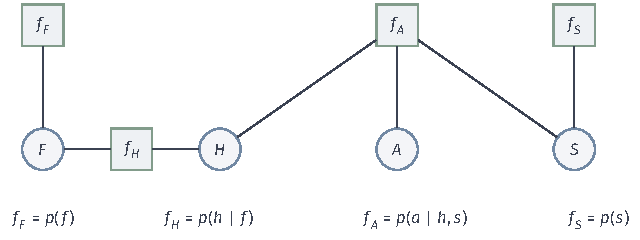
\includegraphics[width=108.433mm]{figures/06-probabilistic-graphical-models/01-representation/tikz/pgm-representations-alarm-factor-graph/figure.pdf}
  \caption{报警模型的四因子表示。圆形表示随机变量，方形表示局部条件分布或先验函数；$f_H$使用$F,H$，$f_A$使用$H,A,S$，连线记录函数的输入变量。}
  \label{fig:pgm-representations-alarm-factor-graph}
\end{figure}

Markov网络的每个势也对应一个因子节点，连接所有作用域变量。边势和一元势可以各自保留为小因子，无需预先合成极大团表。将每个因子的输入变量两两连接，又可得到无向变量图；该图记录共同作用域，但不再区分它由多少个局部函数组成。

三个二元势相乘的$g=\psi_{\{1,2\}}\psi_{\{2,3\}}\psi_{\{1,3\}}$生成一个无向三角形，一般三元势$\psi_{\{1,2,3\}}$也对应同一个团。前者明确分为三个二元函数，后者可能包含不可约的三元作用。三角形本身没有条件独立性来区分两种表示，因子图却显示了局部函数的数量和阶数。这些额外信息来自输入函数的分解。

\subsection{表示的非唯一性}
\label{sec:pgm-representations-nonuniqueness}

合并局部函数会改变因子图，而整个函数可以保持原样。图~\ref{fig:pgm-representations-factor-grouping}将三个二元因子相乘为一个三元因子，六边环随之变成星形。星形虽无环，中心表却从单个二元因子的$r^2$项变为$r^3$项。计算开销因此需要同时看连接结构与因子大小。

\begin{figure}[htbp]
  \centering
  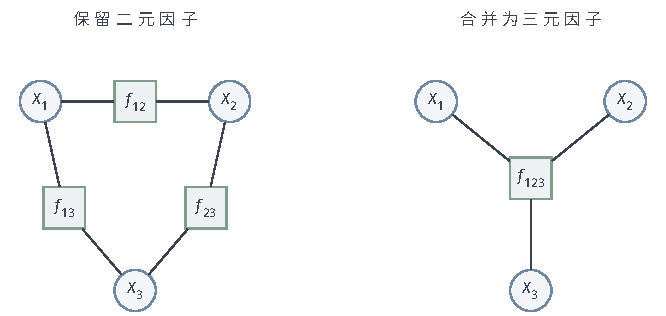
\includegraphics[width=112.000mm]{figures/06-probabilistic-graphical-models/01-representation/tikz/pgm-representations-factor-grouping/figure.pdf}
  \caption{合并因子前后的同一联合函数。左图由三个二元因子构成环，右图以$f_{123}=f_{12}f_{23}f_{13}$形成一个三元因子的星形。两种因子图都生成三角形变量图，局部表规模与连接结构不同。}
  \label{fig:pgm-representations-factor-grouping}
\end{figure}

函数相乘可以合并，能否拆分则要看函数值。若二元函数可以写成两个一元函数的乘积，即满足
\[
  f_{12}(x_1,x_2)=u(x_1)v(x_2),
\]
它的离散函数表就是外积，秩至多为$1$。式~\eqref{eq:pgm-representations-cycle-potentials}的表$\left(\begin{smallmatrix}2&1\\1&2\end{smallmatrix}\right)$行列式为$3$，无法写成两个一元函数的乘积。三元势拆成三个二元势时，同样需要核验具体函数是否具有相应结构。

共享变量还允许在两个因子间转移权重，同时保持总乘积。这种\term{重新参数化}（reparameterization）可以保留原作用域。例如用严格正的$h(x_2)$定义
\[
  \widetilde f_{12}=f_{12}h(x_2),\qquad
  \widetilde f_{23}=\frac{f_{23}}{h(x_2)}.
\]
两新因子的$h$恰好约去，总乘积与原来相同。若仅将一个因子乘以正常数，未归一化函数$g$便同比缩放，调整$Z$后仍得到同一分布$p$。前一种变换保留联合函数，后一种保留归一化分布，二者的代数要求不同。

变量节点的删除也能从因子图读出一些独立性。设$A,B,S\subseteq V$两两不交，$A,B$非空。对非负概率因子分解，删除\emph{变量节点}$S$后，若$A$与$B$分处不同连通分量，给定$\bm{X}_S=\bm{s}$便可按分量整理乘积，并分别归一化，得到$\bm{X}_A\perp\bm{X}_B\mid\bm{X}_S$。运算使用条件分布有效的$\bm{s}$；有限离散情形要求$p(\bm{X}_S=\bm{s})>0$。该分离提供充分保证，具体函数还可能隐含其他独立性。

报警因子图一直有连接$H-f_A-S$，函数却满足$\sum_a f_A(h,a,s)=1$，消去报警后，两原因仍然边缘独立。这条条件归一化等式保留在函数内，拓扑没有显示它。因子图适合据作用域安排计算；碰撞关系仍需原有向图的条件语义，无向Markov约束则由相应变量图的分离判断。

\subsection{因子图上的局部计算}
\label{sec:pgm-representations-local-computation}

有了因子图，就可以在它上面组织推断计算了。本章只说明最基本的局部操作如何由图的连接决定，具体的消元顺序选择、复杂度分析和消息复用留给第~\ref{chap:pgm-elimination}章与第~\ref{chap:pgm-junction-tree}章。先从最常见的问题说起：观测到一部分变量后，想求另一部分（查询）变量的后验分布，就要把既未观测、也不查询的变量全部求和消去。下面的局部计算采用有限离散取值变量和有限个非负实值因子，乘积可以归一化为合法分布。所给证据满足$p(\bm X_S=\bm s)>0$。这些条件保证下面的求和都是有限和，后验归一化分母为正，有限候选集上的最大值也能取得。一般函数的因子图定义本身不要求变量离散；连续查询还需另行处理积分、条件密度版本以及最大值是否取得，不能仅靠下述有限运算公式得到这些保证。

观测$\bm{X}_S=\bm{s}$后，将相关因子中的证据坐标固定在该值。以$Q\subseteq V\setminus S$为查询集，其他待消变量组成$R=V\setminus(Q\cup S)$。将它们求和消去，得到查询的未归一化边缘函数：
\begin{equation}
  \widetilde p(\bm{x}_Q,\bm{s})
  =\sum_{\bm{x}_R}
  \prod_{\alpha\in\mathcal{F}}
  f_\alpha(\bm{x}_{D_\alpha\setminus S},\bm{s}_{D_\alpha\cap S}).
  \label{eq:pgm-representations-marginal-query}
\end{equation}
若$p(\bm{s})>0$，对$\bm{x}_Q$求和得到的常数可将$\widetilde p$归一化，得到后验边缘分布。

分配律使每步计算可以只处理相关因子：$u$不含$x_i$时，有$\sum_{x_i}u\,v=u\sum_{x_i}v$。因此，收集与$x_i$相连的因子，相乘再求和，将所得新函数接到剩余作用域即可。式~\eqref{eq:pgm-representations-cycle-message}就是将两个边因子经消元变为$\{1,3\}$上的新因子。连接关系由此给出每步的输入函数及输出变量集。

求后验边缘回答的是“各状态分别有多可能”，但很多实际问题要的不是概率，而是“最可能的完整情形是什么”：如图像分割中要给出一整幅最可能的标签配置，故障诊断中要给出一组最可能的状态。这时汇总未知变量的算子要从“求和”换成“取最大值”。寻找全部非证据变量的最可能联合配置时，改对其完整配置取最大值：
\[
  \max_{\bm{x}_{V\setminus S}}
  \prod_{\alpha\in\mathcal{F}}f_\alpha.
\]
该查询称为\term{最可能解释}（most probable explanation, MPE）。$Z$对所有候选配置相同，最大化未归一化权重就能比较候选；每步记录取得最大值的状态，结束后回溯，才能恢复最优配置。若仅对部分变量求最优，其他未观测变量需先求和，则形成\term{边缘最大后验推断}（marginal maximum a posteriori inference, marginal MAP）问题。沿用查询集$Q$与其余待消集$R$，它寻找的是
\begin{equation}
  \bm x_Q^\star\in
  \argmax_{\bm x_Q}\left\{
    \sum_{\bm x_R}
    \prod_{\alpha\in\mathcal F}
      f_\alpha(\bm x_{D_\alpha\setminus S},
        \bm s_{D_\alpha\cap S})
  \right\}.
  \label{eq:pgm-representations-marginal-map}
\end{equation}
内层求和汇总没有被选作优化目标的变量，外层最大化再选择查询配置；证据的归一化常数不随$\bm x_Q$改变，所以不影响这个选择。边缘概率查询输出每个查询配置的后验概率，MPE输出全部非证据变量的最优联合配置，边缘MAP则输出查询变量的最优配置。这三个任务保留和消去的信息不同。

边缘MAP混合求和与最大化，两种算子的先后次序会影响结果。用一个人工构造的严格正二元概率表即可看出差别：以$x=0,1$为行、$y=0,1$为列，取
\[
  \bigl[p(x,y)\bigr]=
  \begin{pmatrix}
    0.36&0.04\\
    0.30&0.30
  \end{pmatrix}.
\]
四项之和为$1$，MPE选择最大单格$(x,y)=(0,0)$，概率为$0.36$。若只希望选择$x$，两行的边缘概率分别是$0.40$与$0.60$，边缘MAP便选择$x=1$。先求和再取最大值得到$\max_x\sum_y p(x,y)=0.60$；若颠倒次序，两列最大值相加却得到$\sum_y\max_x p(x,y)=0.36+0.30=0.66$。后一个计算允许第一列选$x=0$、第二列选$x=1$，不再要求同一个$x$配置解释全部$y$状态，因此改变了原查询。

一般混合查询不能任意交换这两个算子，但作用域相互分开时可能提前处理某个最大化。例如固定其余变量$\bm z$后，若乘积为$h(x,\bm z)u(y,\bm z)$，非负性使
\[
  \max_x\sum_y h(x,\bm z)u(y,\bm z)
    =\bigl[\max_x h(x,\bm z)\bigr]
      \bigl[\sum_y u(y,\bm z)\bigr].
\]
这里$h$不含$y$、$u$不含$x$，所以$x$的最佳选择不随被汇总的$y$改变。是否合法换序，要检查当前相关因子的作用域；一个通用的正确顺序是先消去全部$R$，再最大化$Q$，具体图结构可能允许更多安排。

边缘概率查询和完整配置MPE都用乘法组合函数，区别在于汇总状态的算子：\term{和积}（sum-product）随后求和，\term{最大积}（max-product）随后取最大值。在四环的式~\eqref{eq:pgm-representations-cycle-message}中，将求和换为最大化，两端相同时得到$4$，不同时得到$2$；原来的求和结果则为$5$和$4$。输入因子相同，消元算子决定了当前函数回答的是概率汇总还是最优权重。边缘MAP同时使用两种汇总，仍需保留刚才说明的顺序约束。

和积与最大积两套计算的步骤几乎完全相同：都是收集相邻因子加以组合，再对待消变量的取值做汇总，唯一区别是组合用乘法、汇总分别用求和或取最大值。既然流程相同，可将其抽象成一种统一形式，使同一套消息传递实现只需替换两个运算就能服务不同查询；这种抽象还能说明“合法重组”依赖哪些代数性质。将组合函数与汇总状态两项操作抽象出来，就得到\term{半环}（semiring）形式：以$\otimes$组合局部函数，以$\oplus$汇总待消变量的不同取值。采用交换半环时，两运算都满足结合律、交换律，$\otimes$对$\oplus$还满足分配律。以$e_\oplus$记$\oplus$的单位元、$e_\otimes$记$\otimes$的单位元，并有吸收关系$a\otimes e_\oplus=e_\oplus$。这组运算条件让收集因子后的消元写成
\begin{equation}
  \begin{aligned}
    h(\bm{x}_{D\setminus\{i\}})
    &=
    \bigoplus_{x_i}
    \ \bigotimes_{\alpha:\,i\in D_\alpha}
    f_\alpha(\bm{x}_{D_\alpha}),\\
    D&=\bigcup_{\alpha:\,i\in D_\alpha}D_\alpha.
  \end{aligned}
  \label{eq:pgm-representations-semiring-elimination}
\end{equation}
在非负实数上，$(\oplus,\otimes)=(+,\times)$就是和积，其$(e_\oplus,e_\otimes)=(0,1)$；最大积用$(\max,\times)$，单位元也为$0$和$1$。取对数后，在$\mathbb{R}\cup\{-\infty\}$上使用$(\max,+)$，有$(e_\oplus,e_\otimes)=(-\infty,0)$，零权重变为$-\infty$。每种运算都具备上述分配关系，所以同样的收集因子、局部消元步骤可以用于相应的纯和积或纯最大积查询\scite{pgm-overview-kschischang2001}。这里每次汇总只有有限项，普通半环的公理已足以支持重组；若要进行无穷汇总或连续积分，还需相应的收敛与交换运算条件。一个固定的交换半环也不会自动消除边缘MAP混用求和与最大化的顺序限制。

一次消元留下剩余变量上的函数，它概括了被消变量对后续计算的影响。沿图传递这样的函数，就是消息传递的基本操作。在无环因子图上，移除一条边将计算分成不重叠的两部分，一侧的消息能汇总该侧全部影响，因而和积可精确求边缘。有环图反复更新消息时，传回的信息可能已包含先前从当前节点发出的影响，两侧不再分离；后文的环置信传播将讨论这一问题。另一种精确组织是先按顺序消元形成大团，再在团之间安排消息。第~\ref{chap:pgm-elimination}章讨论消元顺序与复杂度，第~\ref{chap:pgm-junction-tree}章介绍消息的组织及复用。

\section{本章小结}
\label{sec:pgm-representations-summary}

图转换会同时涉及分布值、独立性声明和计算结构，三者需分别比较。I-map要求图声明属于分布的真实独立性，即$\mathcal{I}(\mathcal{G})\subseteq\mathcal{I}(p)$，D-map方向相反。当前查询的祖先道德图精确复现d-分离，整图道德化通常减少可见的独立性。碰撞结构与无弦四环分别展示两类图完美表示的边界；弦图与父集成团的有向图则可互相保留全部图分离关系。

祖先道德图将查询两侧的因子分开归一化，从而证明d-分离的可靠性。对未分离查询，离散条件表与线性高斯参数的非平凡多项式提供相容分布中的依赖见证，给出这两个模型类的完备性。若一个固定分布的全部独立性都要对应图的d-分离，还需忠实性，将模型类的存在保证加强到该分布的完美映射。

局部函数的重组可以保留完整分布：有向条件因子成为道德图的团势，弦图团势沿完美消元序生成条件表，非弦图则借填充边容纳中间函数。四环的数值计算中，新增边让图少声明一项独立性，原函数却继续满足它。只有允许新条件表各自自由变化，转换后的完整图模型族才更大。

因子图用变量与函数的连接保留输入分解，按查询选择求和或最大化，实现局部组合与消元。同一分布有多种因子图，连接方式和局部函数的阶数共同决定开销。给定因子和查询后，接下来的任务是选择消元顺序，控制中间函数的大小，并复用已完成的局部计算。

\paragraph{扩展阅读}
Koller与Friedman的教材系统比较有向、无向及因子化表示。书中的转换例子可结合本章的三项比较继续阅读：哪些联合概率保持原样，哪些独立性仍由新图保证，以及局部函数的重组怎样影响推断所需的中间表\scite{pgm-koller2009}。

\chapter{基于变量消除的精确推断}
\label{chap:pgm-elimination}

设备报警后，诊断任务可以有两种输出：给出故障的后验概率，或选出一组最可能的故障、过热和传感器状态。两种输出使用同一组局部因子，却以不同方式汇总未知状态。本章从第~\ref{sec:pgm-representations-local-computation}节的因子组合与消元操作出发，给出完整算法及其正确性证明。对$d$个二元变量，直接枚举需访问$2^d$个配置；利用局部分解减少重复计算，是精确推断的主要任务。

查询通常只保留部分变量，其余变量的影响可以汇总成剩余变量上的函数，供后续步骤使用。\term{变量消除}（variable elimination, VE）据此逐个收集含有当前变量的因子，将它们相乘，再以求和、积分或最大化消去该变量；所得新因子替换桶内函数，保存它们对剩余变量的共同影响。本章分别说明替换为何保留查询答案、查询为何选择不同算子，以及顺序怎样改变中间作用域。离散因子以状态组合数表示规模，高斯因子则以矩阵块维度表示规模，两种表示由此产生不同的计算代价。

\section{推断问题与因子运算}
\label{sec:pgm-elimination-factor-operations}

\subsection{查询、证据与消元变量}
\label{sec:pgm-elimination-query-evidence}

求故障后验时，要固定报警证据，保留故障变量，并汇总其余未知状态。一般地，模型的节点集合为$V$，节点$i$对应随机变量$X_i$；已观测节点组成$O\subseteq V$，取值为$\bm{x}_O=\bm{e}$，查询节点组成$Q\subseteq V\setminus O$。待消元节点为$R=V\setminus(O\cup Q)$。三个大写集合指定变量角色，$\bm{x}_Q$才是一组查询状态。证据集合用$O$记，以便与图的边集合$E$区分。

以下把模型参数视为已知输入。设共有$m$个非负因子$\psi_a$，其完整乘积具有有限且非零的归一化常数$Z$，联合分布写为
\begin{equation}
  p(\bm{x})=\frac{1}{Z}\prod_{a=1}^{m}\psi_a(\bm{x}_{S_a}),
  \qquad S_a\subseteq V.
  \label{eq:pgm-elimination-factorization}
\end{equation}
有向模型采用局部条件概率作为因子，完整积已归一化，故$Z=1$。无向模型的势需由全局$Z$归一化。这些函数都是当前推断的输入，第~\ref{chap:pgm-parameter-learning}章再讨论如何从数据估计它们。

把证据坐标固定在观测值后，原乘积成为未观测变量上的函数：
\begin{equation}
  F_{\bm{e}}(\bm{x}_{V\setminus O})
  =\left.\prod_{a=1}^{m}\psi_a(\bm{x}_{S_a})
  \right|_{\bm{x}_O=\bm{e}}.
  \label{eq:pgm-elimination-evidence-function}
\end{equation}
先取各变量状态数有限的离散情形。汇总$R$的联合状态得到查询权重，再对$Q$的所有状态归一化：
\begin{equation}
  \begin{aligned}
    g_Q(\bm{x}_Q)
      &=\sum_{\bm{x}_R}F_{\bm{e}}(\bm{x}_Q,\bm{x}_R),\\
    Z_{\bm{e}}&=\sum_{\bm{x}_Q}g_Q(\bm{x}_Q),\\
    p(\bm{x}_Q\mid\bm{e})&=\frac{g_Q(\bm{x}_Q)}{Z_{\bm{e}}}.
  \end{aligned}
  \label{eq:pgm-elimination-marginal-query}
\end{equation}
下标$\bm{x}_R$遍历待消元变量的联合状态。总权重满足$Z_{\bm{e}}=Zp(\bm{e})$，因此计算条件概率时原$Z$在分子分母中抵消，可以直接从因子积开始。后验比值在$Z_{\bm{e}}>0$的证据事件上有定义；模型赋予观测零概率时，该比值的分母为零。

连续变量用积分汇总未知坐标。联合密度存在且积分有限时，式~\eqref{eq:pgm-elimination-marginal-query}的积分版本给出边缘条件密度。连续观测处的$p(\bm{e})$表示边缘密度值，比值只在密度有限且为正的观测处使用。形式相同的查询还需配合适当的函数表示，才能解析完成积分。

\subsection{因子乘积}
\label{sec:pgm-elimination-factor-product}

相乘两张因子表时，需要按变量身份及状态含义对齐坐标。\term{作用域}（scope）指定因子的自变量，也指定消元后需要保留的坐标。若$D_i$是$X_i$的取值集合，作用域为$S$的离散因子是非负函数$\psi_S:\prod_{i\in S}D_i\to[0,\infty)$。存储表时还要记下$S$内变量的排列和状态编码：同一变量可以位于不同表轴上，但相乘时同一个状态必须有相同含义。

两个函数分别使用$A$与$B$中的变量，乘积便使用它们的并集$A\cup B$：
\begin{equation}
  (\psi_A\psi_B)(\bm{x}_{A\cup B})
  =\psi_A(\bm{x}_A)\psi_B(\bm{x}_B).
  \label{eq:pgm-elimination-product}
\end{equation}
对$A\cup B$的一组取值，两因子各读取自己的坐标，其中共享变量取同一状态。例如，$\psi_{\{F,H\}}(f,h)\psi_{\{H,S\}}(h,s)$以$(f,h,s)$为索引；计算$(0,1,0)$时，分别读取前表$(0,1)$与后表$(1,0)$。三个变量均为二元时，两张$4$项表的乘积共有$8$项，新增的坐标来自两表作用域的并集。

因子保存相对权重，其全表求和可以异于$1$。空作用域的因子是标量，也参与完整乘积；条件概率比较中的公共尺度可约去，而证据概率或绝对得分需要这些尺度。乘积还要保留函数的出现次数：两个数值相同的因子仍相乘两次。以下的$\mathcal{F}$因此按多重集合使用。

\subsection{因子约简与边缘化}
\label{sec:pgm-elimination-reduction-marginalization}

观测把一个变量的状态固定后，可以从因子表读取相应切片。把证据代入并从作用域移去固定坐标，称为\term{因子约简}（factor reduction）。报警证据$A=1$将$p(a\mid h,s)$变为$\ell_A(h,s)=p(A=1\mid h,s)$，表示各$(h,s)$状态对该报警的支持权重。结合先验与其他因子、再统一归一化，才能得到这些原因的后验分布。

对状态仍未知的变量，概率查询要汇总其全部取值。\term{边缘化}（marginalization）把这些权重相加，留下其余坐标上的函数：若$i\in S$，则
\begin{equation}
  (\mathop{\textstyle\sum}_{x_i}\psi_S)
    (\bm{x}_{S\setminus\{i\}})
  =\sum_{x_i\in D_i}\psi_S(\bm{x}_{S\setminus\{i\}},x_i).
  \label{eq:pgm-elimination-factor-marginal}
\end{equation}
约简读取已知状态下的切片，边缘化累加未知状态。两种操作都减少自变量数，分别保留观测条件下的权重与未知变量的总贡献。

一个未知变量可能同时影响多个因子，汇总时需要让它们共享同一个状态。若$X_i$同时出现在$\psi_1(x_i,y)$和$\psi_2(x_i,z)$中，先将因子相乘，再对共同的$x_i$求和，所得新因子为
\[
  \sum_{x_i}\psi_1(x_i,y)\psi_2(x_i,z)\text{。}
\]
分别求和后相乘，会允许两张表使用不同的$x_i$，改变原函数的共享坐标约束。因此，消元先收集所有含$X_i$的因子，再对共同乘积汇总；新函数保留它们在剩余坐标上的联合影响。

完成非查询变量的边缘化后，查询权重可以统一归一化。中途若用一个与全部自变量无关的正常数缩放因子，最终条件概率的公共尺度仍会抵消，但计算$Z_{\bm{e}}$需记录并补回该常数。逐行归一化的除数随剩余坐标变化，会改变各查询配置的相对权重，因而属于对函数的实质修改。

\section{边缘概率的变量消除算法}
\label{sec:pgm-elimination-sum-product}

\subsection{从朴素枚举到分配律}
\label{sec:pgm-elimination-distributivity}

沿用报警模型作为可逐项计算的例子：故障$F$、过热$H$、报警$A$和传感器失灵$S$均取$0$或$1$。联合分解为
\begin{equation}
  p(f,h,a,s)=p(f)p(h\mid f)p(s)p(a\mid h,s).
  \label{eq:pgm-elimination-alarm-model}
\end{equation}
有向结构$F\to H\to A\leftarrow S$使两个根节点$F,S$独立。设置$p(F=1)=0.1$、$p(S=1)=0.05$，并取
\[
  p(H=1\mid F=0)=0.1,\qquad
  p(H=1\mid F=1)=0.8.
\]
表~\ref{tab:pgm-elimination-alarm-cpt}给出四种$(h,s)$下的报警概率；二元分布的状态$0$概率都由$1$减去状态$1$概率得到。这组人工参数只用于解释消元步骤。

\begin{table}[htbp]
  \centering
  \begin{tabular}{ccc}
    \toprule
    $h$ & $s$ & $p(A=1\mid h,s)$\\
    \midrule
    $0$ & $0$ & $0.01$\\
    $1$ & $0$ & $0.90$\\
    $0$ & $1$ & $0.70$\\
    $1$ & $1$ & $0.99$\\
    \bottomrule
  \end{tabular}
  \caption{报警模型的人工条件表。每行固定$(h,s)$并列出$p(A=1\mid h,s)$，同一行的不报警概率为$1-p(A=1\mid h,s)$。}
  \label{tab:pgm-elimination-alarm-cpt}
\end{table}

将$A=1$代入报警因子后，故障查询需要累加过热和传感器的全部状态：
\[
  g_F(f)=\sum_h\sum_s p(f)p(h\mid f)p(s)\ell_A(h,s).
\]
直接枚举对每个$f$访问全部$(h,s)$，共需访问$8$个三元配置。其中$p(s)\ell_A(h,s)$不使用$f$，可以让两种故障状态共享这部分结果。利用乘法对加法的分配律，先对$s$汇总与它相关的两个函数：
\begin{equation}
  g_F(f)
  =p(f)\sum_h p(h\mid f)
    \underbrace{\sum_s p(s)\ell_A(h,s)}_{\tau_S(h)}.
  \label{eq:pgm-elimination-alarm-reorder}
\end{equation}
所得$\tau_S(h)$替换$p(s)$与$\ell_A(h,s)$，对每种$h$计算一次，供所有$f$使用。下一步将$p(h\mid f)\tau_S(h)$对$h$求和，生成$f$上的函数。图~\ref{fig:pgm-elimination-alarm-buckets}将每步输入与输出的坐标分别画出。

\begin{figure}[htbp]
  \centering
  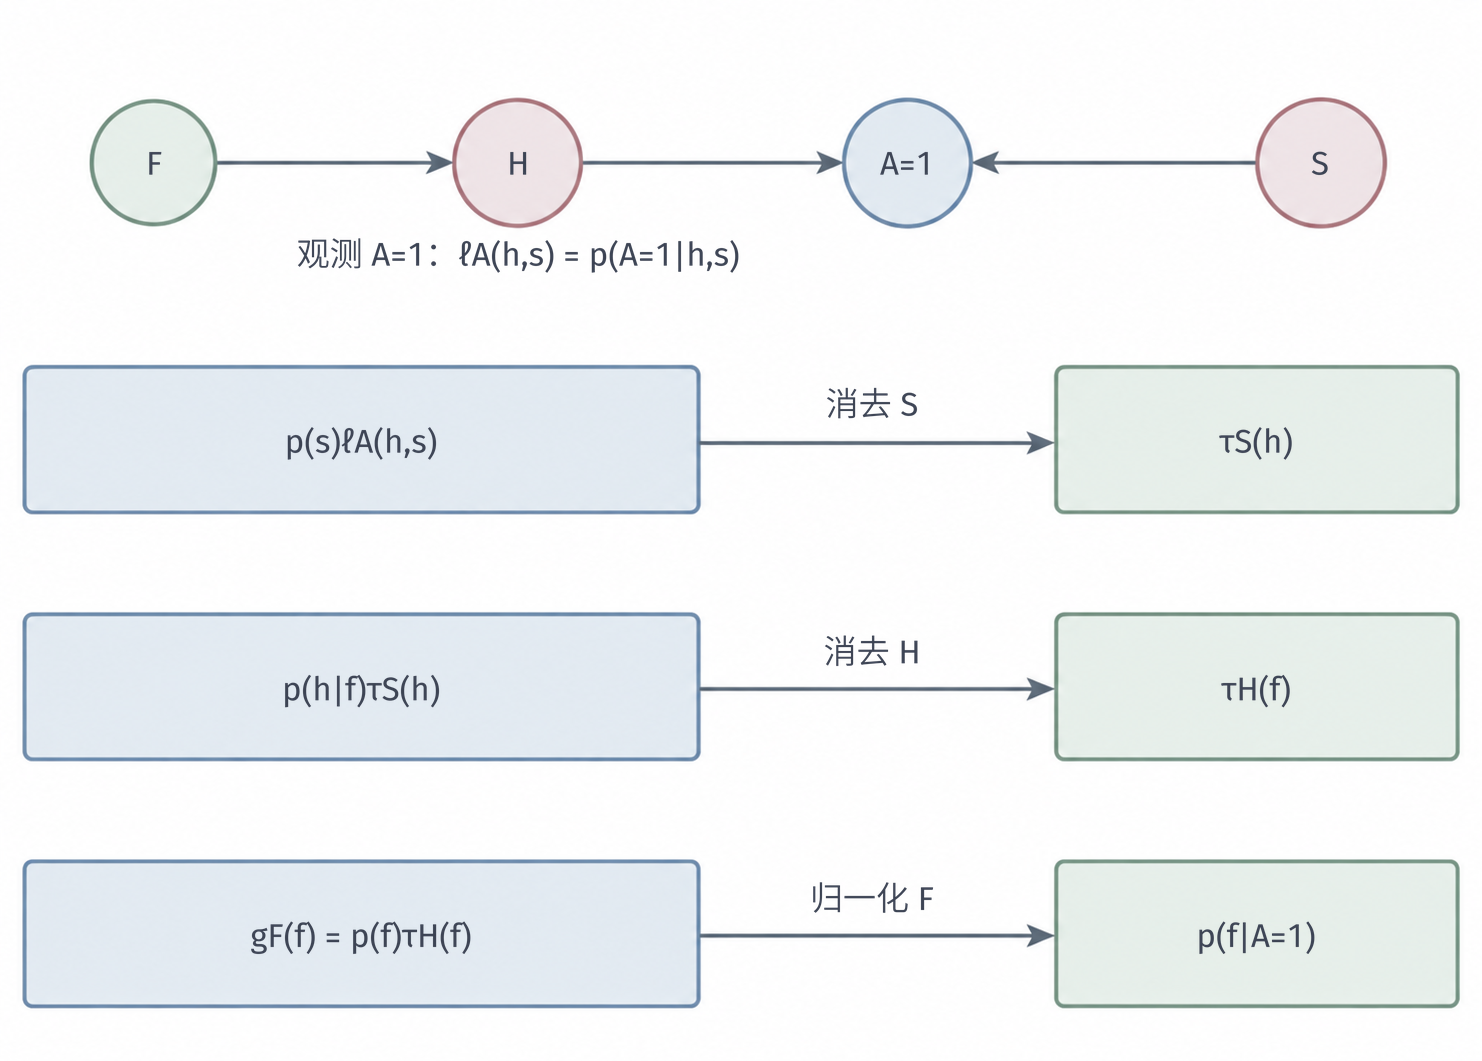
\includegraphics[width=112.000mm]{figures/06-probabilistic-graphical-models/02-inference/generated/pgm-elimination-alarm-buckets/figure.png}
  \caption{故障后验查询的两步消元。上方有向图以蓝色$A=1$标出证据；下方先从$p(s)\ell_A(h,s)$求和得到$\tau_S(h)$，再从$p(h\mid f)\tau_S(h)$求和得到$\tau_H(f)$。每步输出只保留尚未消去的坐标，$F$最终结合$p(f)$并归一化。}
  \label{fig:pgm-elimination-alarm-buckets}
\end{figure}

这种重排让后续故障状态复用同一局部汇总，每个$s,h$状态仍以原权重参与求和，所以代数结果与完整枚举相同。节省多少取决于输出函数的作用域：若一桶包含几乎全部剩余变量，形成的新表仍可能过大。选择顺序的目的，就是控制这类中间函数的坐标数和状态组合数。

\subsection{变量消除算法}
\label{sec:pgm-elimination-ve-algorithm}

一般因子分解也按同一方式替换局部乘积。证据约简后的初始因子多重集合记为$\mathcal{F}^{(0)}$，顺序$\pi=(i_1,\ldots,i_k)$将待消元集合$R$的每个节点列出恰好一次。第$t$步收集全部含$X_{i_t}$的因子：
\[
  \mathcal{B}_t
  =\{\psi\in\mathcal{F}^{(t-1)}:
      i_t\in\operatorname{scope}(\psi)\}.
\]
$\operatorname{scope}(\psi)$给出函数的作用域。当前收集的多重集合称为变量的\term{桶}（bucket），其中的函数需要共同参与本步求和。令$U_t$为它们作用域的并集，去掉当前变量后的集合为$N_t=U_t\setminus\{i_t\}$，局部更新写为
\begin{equation}
  \begin{aligned}
    \phi_t(\bm{x}_{U_t})&=\prod_{\psi\in\mathcal{B}_t}\psi,\\
    \tau_t(\bm{x}_{N_t})&=\sum_{x_{i_t}}\phi_t(\bm{x}_{U_t}).
  \end{aligned}
  \label{eq:pgm-elimination-local-sum}
\end{equation}
计算$\phi_t$时，先按式~\eqref{eq:pgm-elimination-product}对齐每个函数的坐标。桶外函数不含$X_{i_t}$，从本步求和提出后仍留在当前集合中。

\begin{algorithm}[离散边缘概率的变量消除]
  \label{alg:pgm-elimination-marginal}
  \begin{algorithmic}[1]
    \Require 非负有限因子$\{\psi_a\}$，证据$\bm{x}_O=\bm{e}$，查询集$Q$
    \Require $R=V\setminus(O\cup Q)$的排列$\pi=(i_1,\ldots,i_k)$
    \Ensure 查询因子$g_Q$及$Z_{\bm{e}}>0$时的条件分布
    \State 将证据代入各因子，得到$\mathcal{F}^{(0)}$；保留标量因子
    \State 对未出现在任何作用域中的未观测变量，加入其恒为$1$的一元因子
    \For{$t=1,\ldots,k$}
      \State 收集$\mathcal{B}_t$，令$U_t$为其作用域的并集
      \State 对齐坐标并求乘积$\phi_t=\prod_{\psi\in\mathcal{B}_t}\psi$
      \State 对$x_{i_t}$求和，得到$\tau_t(\bm{x}_{U_t\setminus\{i_t\}})$
      \State $\mathcal{F}^{(t)}\gets
        (\mathcal{F}^{(t-1)}\setminus\mathcal{B}_t)\cup\{\tau_t\}$
    \EndFor
    \State 在查询取值空间上计算$g_Q=\prod_{\psi\in\mathcal{F}^{(k)}}\psi$
    \State 计算$Z_{\bm{e}}=\sum_{\bm{x}_Q}g_Q(\bm{x}_Q)$
    \If{$Z_{\bm{e}}=0$}
      \State 返回证据与模型不相容，条件分布未定义
    \Else
      \State 返回$g_Q$、$Z_{\bm{e}}$及$g_Q/Z_{\bm{e}}$
    \EndIf
  \end{algorithmic}
\end{algorithm}

算法~\ref{alg:pgm-elimination-marginal}按出现次数移除桶内函数并加入新因子。若某个未观测变量未进入任何函数，加入恒为$1$的一元因子后，它的求和仍贡献状态数。$R=\varnothing$时没有消元步骤，$Q=\varnothing$时最终乘积是证据权重标量$Z_{\bm{e}}$。边缘查询输出汇总后的函数，各个已消变量的状态都参与了累加，因此输出无需配置回溯。

报警查询从$p(f)$、$p(h\mid f)$、$p(s)$和$\ell_A(h,s)$四因子开始。$S$桶由$p(s)$与$\ell_A(h,s)$组成，两种$h$下的新函数值分别为
\begin{equation}
  \begin{aligned}
    \tau_S(0)&=0.95\times0.01+0.05\times0.70=0.0445,\\
    \tau_S(1)&=0.95\times0.90+0.05\times0.99=0.9045.
  \end{aligned}
  \label{eq:pgm-elimination-alarm-s}
\end{equation}
用$\tau_S(h)$替换$S$桶后，当前集合为$\{p(f),p(h\mid f),\tau_S(h)\}$。接着将含$H$的两个函数相乘并求和，得到
\begin{equation}
  \begin{aligned}
    \tau_H(0)&=0.9\times0.0445+0.1\times0.9045=0.1305,\\
    \tau_H(1)&=0.2\times0.0445+0.8\times0.9045=0.7325.
  \end{aligned}
  \label{eq:pgm-elimination-alarm-h}
\end{equation}
余下$p(f)$与$\tau_H(f)$相乘，给出$g_F(0)=0.11745$、$g_F(1)=0.07325$，总权重为$0.19070$。原有向联合积的$Z=1$，因此此值也是证据概率$p(A=1)$。把故障状态$1$的权重除以总权重，得到
\begin{equation}
  p(F=1\mid A=1)
  =\frac{0.07325}{0.19070}
  \approx0.384111.
  \label{eq:pgm-elimination-alarm-posterior}
\end{equation}
报警使故障概率从$0.1$升至约$0.384$。无故障过热、传感器失灵以及小概率误报也能解释报警，它们的概率都进入求和分母；保留这些解释使后验仍低于$1$。

这个顺序只产生$\tau_S(h)$、$\tau_H(f)$两张一元表。变量较多的模型可先按消元顺序分桶：将输入因子交给作用域中最早待消的变量，每步新函数再交给后续相应桶。这种收集、合并、汇总的组织方式对应Dechter的桶消除算法\scite{pgm-elimination-dechter1999}

\subsection{多变量查询}
\label{sec:pgm-elimination-multivariate-query}

联合查询故障与传感器状态时，保留$Q=\{F,S\}$，仅消去$H$。所需结果使用$(f,s)$共同索引：
\begin{equation}
  g_{F,S}(f,s)
  =p(f)p(s)\sum_h p(h\mid f)\ell_A(h,s).
  \label{eq:pgm-elimination-joint-query}
\end{equation}
以$f=s=0$为例，先汇总两种过热状态，得到
\[
  \begin{aligned}
    g_{F,S}(0,0)
    &=0.9\times0.95\times(0.9\times0.01+0.1\times0.90)\\
    &=0.084645.
  \end{aligned}
\]
对其余三种$(f,s)$执行相同求和，即得到表~\ref{tab:pgm-elimination-joint-query}。

\begin{table}[htbp]
  \centering
  \begin{tabular}{ccc}
    \toprule
    $f$ & $g_{F,S}(f,0)$ & $g_{F,S}(f,1)$\\
    \midrule
    $0$ & $0.084645$ & $0.032805$\\
    $1$ & $0.068590$ & $0.004660$\\
    \bottomrule
  \end{tabular}
  \caption{报警证据下的未归一化$(F,S)$联合权重。四项共用归一化常数$0.19070$，得到$p(f,s\mid A=1)$；若各行分别归一化，则得到给定$f$后的传感器条件分布。}
  \label{tab:pgm-elimination-joint-query}
\end{table}

四项总权重为$0.19070$，各行之和是$g_F(f)$，各列之和是$g_S(s)$。虽然$F,S$观测前独立，报警后的两种原因相互影响：一种解释的后验权重会改变另一种解释的相对可信度。联合表保留了这种关系，两个一元后验的乘积一般给不出它。显式联合输出还有自身的存储代价；保留的查询变量越多，即使各消元桶较小，最后的联合表也可能很大。

\subsection{连续变量的边缘消除}
\label{sec:pgm-elimination-gaussian}

连续推断同样先乘相关函数再积分；不含当前坐标的因子可以提出积分号，非负可测性允许按Tonelli定理交换积分次序。条件密度还要求总积分有限且为正。一般函数积分后可能无法用有限参数精确保存，因此函数表示决定是否能解析消元。高斯二次指数在乘法和积分下保留同类形式，提供了一个可完整计算的连续例子。

高斯核的自变量记为$\bm{x}\in\mathbb{R}^{q}$。将其写成\term{规范形式}（canonical form），以二次项、一次项及常数项系数保存函数，便于相乘时合并参数：
\begin{equation}
  \psi(\bm{x})
  =\exp\!\left\{-\frac12\bm{x}^{\top}\bm{J}\bm{x}
                  +\bm{h}^{\top}\bm{x}+c\right\}.
  \label{eq:pgm-elimination-gaussian-canonical}
\end{equation}
参数$\bm{J}\in\mathbb{R}^{q\times q}$对称，$\bm{h}\in\mathbb{R}^{q}$，$c$为标量。对均值$\bm{\mu}$、协方差$\bm{\Sigma}$的非退化高斯密度，\term{精度矩阵}（precision matrix）$\bm{J}=\bm{\Sigma}^{-1}$以逆协方差表示二次项，$\bm{h}=\bm{J}\bm{\mu}$，归一化常数进入$c$。局部因子可以在部分方向没有二次约束；所有因子组合后的联合精度要求正定，使完整高斯核可归一化。

规范形式相乘会将指数相加，因此对齐坐标后分别累加$\bm{J}$、$\bm{h}$和$c$即可。不在某因子作用域内的坐标补零，与离散表相乘时扩展坐标的操作对应。吸收证据仍是代入：将变量分为保留块$\bm{x}_A$和观测块$\bm{x}_O=\bm{e}$，参数变为
\[
  \begin{aligned}
    \bm{J}'&=\bm{J}_{A,A},\\
    \bm{h}'&=\bm{h}_A-\bm{J}_{A,O}\bm{e},\\
    c'&=c+\bm{h}_O^{\top}\bm{e}
       -\frac12\bm{e}^{\top}\bm{J}_{O,O}\bm{e}.
  \end{aligned}
\]
这组参数保存固定$\bm{x}_O$后的函数，未观测变量仍全部保留。接下来积分消元才汇总未知坐标的贡献。

一次积分先收集所有含待消变量的因子，将桶积写成式~\eqref{eq:pgm-elimination-gaussian-canonical}。作用域分为待消块$B$和保留块$A$，令$\bm{y}=\bm{x}_B\in\mathbb{R}^{b}$、$\bm{z}=\bm{x}_A\in\mathbb{R}^{a}$，相应参数为
\[
  \bm{J}=
  \begin{pmatrix}
    \bm{J}_{B,B}&\bm{J}_{B,A}\\
    \bm{J}_{A,B}&\bm{J}_{A,A}
  \end{pmatrix},
  \qquad
  \bm{h}=
  \begin{pmatrix}\bm{h}_B\\\bm{h}_A\end{pmatrix}.
\]
关于$\bm{y}$的积分使用正定主块$\bm{J}_{B,B}\succ0$。在非退化联合高斯模型中，完整当前精度和后续Schur补都保持正定。桶已收集全部含$\bm{y}$的二次项，其$B,B$块与完整当前精度的同一主块相同，因而满足该条件。

提取指数中的$\bm{y}$项，得到
\[
  -\frac12\bm{y}^{\top}\bm{J}_{B,B}\bm{y}
  +\bm{y}^{\top}(\bm{h}_B-\bm{J}_{B,A}\bm{z}).
\]
将线性系数记为$\bm{u}(\bm{z})=\bm{h}_B-\bm{J}_{B,A}\bm{z}$。对$\bm{y}$配方，可以分离需要积分的高斯核与保留的$\bm{z}$函数：
\begin{equation}
  \begin{aligned}
    &-\frac12
      \bigl(\bm{y}-\bm{J}_{B,B}^{-1}\bm{u}\bigr)^{\top}
      \bm{J}_{B,B}
      \bigl(\bm{y}-\bm{J}_{B,B}^{-1}\bm{u}\bigr)\\
    &\hspace{2em}
      +\frac12\bm{u}^{\top}\bm{J}_{B,B}^{-1}\bm{u}.
  \end{aligned}
  \label{eq:pgm-elimination-complete-square}
\end{equation}
高斯核的积分为$(2\pi)^{b/2}|\bm{J}_{B,B}|^{-1/2}$，与核中心无关。余项$\bm{u}^{\top}\bm{J}_{B,B}^{-1}\bm{u}/2$依赖保留变量。展开$\bm{u}$，重新收集$\bm{z}$的二次、一次及常数系数，所得参数为
\begin{equation}
  \begin{aligned}
    \bm{J}'&=\bm{J}_{A,A}
      -\bm{J}_{A,B}\bm{J}_{B,B}^{-1}\bm{J}_{B,A},\\
    \bm{h}'&=\bm{h}_A
      -\bm{J}_{A,B}\bm{J}_{B,B}^{-1}\bm{h}_B,\\
    c'&=c+\frac12\bm{h}_B^{\top}\bm{J}_{B,B}^{-1}\bm{h}_B\\
      &\quad+\frac b2\log(2\pi)-\frac12\log|\bm{J}_{B,B}|.
  \end{aligned}
  \label{eq:pgm-elimination-schur}
\end{equation}
积分输出仍写成$\exp\{-\bm{z}^{\top}\bm{J}'\bm{z}/2+\bm{h}'^{\top}\bm{z}+c'\}$。更新矩阵$\bm{J}'$是$\bm{J}_{B,B}$在$\bm{J}$中的\term{Schur补}（Schur complement），其中减去的矩阵项保存了被消块对保留块的影响。取高斯边缘时，协方差表示直接保留相应主块；精度表示则使用这个Schur补。两种更新各对应自己的参数化。

完整当前精度正定还保证它的Schur补正定。对任意$\bm{z}\ne\bm{0}$，选取$\bm{y}=-\bm{J}_{B,B}^{-1}\bm{J}_{B,A}\bm{z}$，其联合二次型为
\[
  \begin{pmatrix}\bm{y}\\\bm{z}\end{pmatrix}^{\top}
  \bm{J}
  \begin{pmatrix}\bm{y}\\\bm{z}\end{pmatrix}
  =\bm{z}^{\top}\bm{J}'\bm{z}>0.
\]
这个正二次型保证最终查询核可以归一化，均值为$(\bm{J}')^{-1}\bm{h}'$，协方差为$(\bm{J}')^{-1}$。论证使用完整联合矩阵；局部桶输出尚需与其它函数组合，本身可以在部分方向没有约束。

均值计算呈现相同的块消元结构。规范形式满足$\bm{J}\bm{\mu}=\bm{h}$，其$B$块给出$\bm{\mu}_B=\bm{J}_{B,B}^{-1}(\bm{h}_B-\bm{J}_{B,A}\bm{\mu}_A)$。代入$A$块便得到$\bm{J}'\bm{\mu}_A=\bm{h}'$。概率边缘化和线性方程消元由此共用Schur补；概率计算另需$c'$中的行列式项，保存积分质量。Lauritzen的教材系统介绍这种高斯消元关系\scite{pgm-lauritzen1996}

\begin{example}[一个二维高斯核的积分]
  \label{ex:pgm-elimination-gaussian-numeric}
  以$\bm{x}=(x_1,x_2)^{\top}$的二次核演示一次更新，设置
  \[
    \bm{J}=\begin{pmatrix}2&-1\\-1&2\end{pmatrix},
    \qquad
    \bm{h}=\begin{pmatrix}1\\0\end{pmatrix},
    \qquad c=0.
  \]
  $\bm{J}$的特征值为$1,3$，完整核因而可归一化。积分消去$x_1$，使用$\bm{J}_{B,B}=2$、$\bm{J}_{B,A}=-1$，式~\eqref{eq:pgm-elimination-schur}给出
  \[
    \bm{J}'=\frac32,\qquad \bm{h}'=\frac12,\qquad
    c'=\frac14+\frac12\log\pi.
  \]
  将这三个参数代回一维核，积分输出为
  \[
    \tau(x_2)=\sqrt{\pi}\exp\!\left\{
      \frac14-\frac34x_2^2+\frac12x_2\right\}.
  \]
  对一维输出配方并归一化，得到$x_2\sim\mathcal{N}(1/3,2/3)$。也可从原联合核计算
  \[
    \bm{J}^{-1}=\frac13
      \begin{pmatrix}2&1\\1&2\end{pmatrix},
    \qquad
    \bm{J}^{-1}\bm{h}=
      \begin{pmatrix}2/3\\1/3\end{pmatrix}.
  \]
  所得联合均值的第二项为$1/3$，协方差第二主块为$2/3$，与积分结果相同。仅取原精度的$\bm{J}_{2,2}=2$会对应方差$1/2$，与正确的边缘方差不同；Schur补中的$1/2$修正项恰好保留了$x_1$的影响。
\end{example}

解析更新依靠二次指数函数在乘法和积分下的闭包性。含离散潜变量时，各离散配置下的高斯经求和通常成为高斯混合，分量数还可能随消元增加；非二次势则需另行分析积分是否仍属于二次指数形式。数值求积或将混合压缩成单高斯，是针对这些情形另引入的近似。

\section{MPE与MAP的变量消除算法}
\label{sec:pgm-elimination-max-product}

两种最优查询的区别在于如何处理未要求作答的变量：MPE对全部未观测变量选出一组联合配置，边缘MAP则先求和汇总非目标变量，再选目标配置。MPE用纯最大化消元，保存每步选择以恢复全部未知状态；边缘MAP的通用正确算法分为先求和、后最大化两阶段，只在第二阶段记录并恢复目标状态。

\subsection{MPE变量消除}
\label{sec:pgm-elimination-mpe}

诊断还可以要求给出一组最有可能的完整解释。\term{最可能解释}（most probable explanation, MPE）在全部非证据变量的联合状态中比较后验权重，每个候选是一组相容的完整配置。令$U=V\setminus O$，目标为
\begin{equation}
  \begin{aligned}
    \bm{x}_U^\star
    &\in\argmax_{\bm{x}_U}p(\bm{x}_U\mid\bm{e})\\
    &=\argmax_{\bm{x}_U}F_{\bm{e}}(\bm{x}_U).
  \end{aligned}
  \label{eq:pgm-elimination-mpe-objective}
\end{equation}
候选配置共用正常数$Z_{\bm{e}}$，因此可直接比较未归一化的$F_{\bm{e}}$寻找最优配置。报告该配置的后验概率时，再用$Z_{\bm{e}}$归一化其权重。

局部最大化使用非负权重的分配关系：与$x_i$无关的乘数可提出最大化算子，
\[
  \max_{x_i}\{\rho(\bm{z})\phi(x_i,\bm{z})\}
  =\rho(\bm{z})\max_{x_i}\phi(x_i,\bm{z}),
  \qquad \rho(\bm{z})\geq0.
\]
沿用VE的收集和替换操作，将桶内求和改为最大化即可得到最优权重。最大值本身没有保存取得它的状态，因此还需\term{回溯表}（backpointer table）：对剩余变量的每组配置，记录当前变量的一个最优取值。局部输出和记录分别为
\begin{equation}
  \begin{aligned}
    \tau_t(\bm{x}_{N_t})
      &=\max_{x_{i_t}}\phi_t(x_{i_t},\bm{x}_{N_t}),\\
    b_t(\bm{x}_{N_t})
      &\in\argmax_{x_{i_t}}\phi_t(x_{i_t},\bm{x}_{N_t}).
  \end{aligned}
  \label{eq:pgm-elimination-max-backpointer}
\end{equation}
多个状态并列时，可按约定顺序选取一个并写入回溯表，由此恢复一个最优配置。若输出需要全部最优配置，则保存全部并列选择，回溯输出的数量也可能很大。

\begin{algorithm}[MPE消元及配置回溯]
  \label{alg:pgm-elimination-mpe}
  \begin{algorithmic}[1]
    \Require 约简后的非负因子$\mathcal{F}^{(0)}$及$U$的排列$\pi$
    \Require 各变量取值有限，$Z_{\bm{e}}>0$，每个变量有对应作用域
    \Ensure 最优配置$\bm{x}_U^\star$及未归一化得分$v^\star$
    \For{$t=1,\ldots,|U|$}
      \State 收集含$X_{i_t}$的因子，形成局部乘积$\phi_t$
      \State 令$N_t=\operatorname{scope}(\phi_t)\setminus\{i_t\}$
      \State 按式~\eqref{eq:pgm-elimination-max-backpointer}计算$\tau_t$和$b_t$
      \State 用$\tau_t$替换桶内因子，并保存$(i_t,N_t,b_t)$
    \EndFor
    \State 将剩余标量因子相乘，得到$v^\star$
    \For{$t=|U|,\ldots,1$}
      \State $x_{i_t}^\star\gets b_t(\bm{x}_{N_t}^\star)$
    \EndFor
    \State 返回$\bm{x}_U^\star$和$v^\star$
  \end{algorithmic}
\end{algorithm}

第$t$步的$N_t$只含当时尚未消去的变量，它们在顺序中晚于$i_t$。按逆序恢复时，这些变量已有取值，能够索引$b_t$并确定$x_{i_t}$。最后一个变量的回溯表以空配置为索引，从它开始逐步查表，即可得到完整配置。

报警模型也可逐桶计算MPE。按$S,H,F$消元，先比较每种$h$下传感器两状态的权重：
\[
  \begin{aligned}
    \tau_S^{\max}(0)&=\max\{0.0095,0.0350\}=0.0350,\\
    \tau_S^{\max}(1)&=\max\{0.8550,0.0495\}=0.8550.
  \end{aligned}
\]
取最大值的状态记录为$b_S(0)=1$、$b_S(1)=0$：$H=0$时失灵传感器的报警权重较大，$H=1$时正常传感器的权重较大。当前尚未确定$H$，所以表中保留两种后续状态各自的选择。

对$H$最大化时，$f=0$下的两候选为$0.9\times0.0350=0.0315$与$0.1\times0.8550=0.0855$，记录$\tau_H^{\max}(0)=0.0855$、$b_H(0)=1$。$f=1$下比较$0.2\times0.0350=0.0070$与$0.8\times0.8550=0.6840$，记录$\tau_H^{\max}(1)=0.6840$、$b_H(1)=1$。最后结合故障先验，比较
\[
  \begin{aligned}
    p(F=0)\tau_H^{\max}(0)&=0.07695,\\
    p(F=1)\tau_H^{\max}(1)&=0.06840.
  \end{aligned}
\]
两候选中$f^\star=0$的权重较大。逆序用$b_H(0)$得到$h^\star=1$，再用$b_S(1)$得到$s^\star=0$，完整解释为$(F,H,S)=(0,1,0)$。代入原因子积，其联合证据权重是$0.9\times0.1\times0.95\times0.9=0.07695$，与最大化结果一致；除以证据概率，后验为约$0.403513$。

模型为无故障但过热的状态赋予正概率，因而$(0,1,0)$是合法候选。它的后验约为$0.404$，表示所有完整候选中最大的单项概率，余下候选仍有总概率。$\tau_t^{\max}$保存最佳完成配置的权重，边缘概率则汇总全部完成配置，两种函数有不同的含义。

算法~\ref{alg:pgm-elimination-mpe}使用有限离散状态，保证每桶可枚举并达到最大值。连续版本还需每次最大值存在且局部优化精确。对正定高斯核，配方式~\eqref{eq:pgm-elimination-complete-square}给出$\bm{y}^\star=\bm{J}_{B,B}^{-1}(\bm{h}_B-\bm{J}_{B,A}\bm{z})$，回溯保存这个关于后续变量的仿射函数；二次项与一次项仍按Schur补更新，常数项则没有积分产生的$(b/2)\log(2\pi)-(1/2)\log|\bm{J}_{B,B}|$。一般连续密度的上确界未必可达到，密度众数还随坐标参数化改变，应按指定密度的众数解释。

\subsection{MAP变量消除}
\label{sec:pgm-elimination-map}

若诊断只选择故障状态，过热与传感器的各种解释需先汇总到每个故障候选中。\term{边缘最大后验推断}（marginal maximum a posteriori inference, marginal MAP）据此寻找部分目标变量的联合后验众数：对其它未观测变量求和，再比较目标状态。记目标集合为$M\subseteq V\setminus O$，待求和集合为$R=V\setminus(O\cup M)$，目标写为
\begin{equation}
  \bm{x}_M^\star
  \in\argmax_{\bm{x}_M}\sum_{\bm{x}_R}
       F_{\bm{e}}(\bm{x}_M,\bm{x}_R).
  \label{eq:pgm-elimination-map-objective}
\end{equation}
取$M=V\setminus O$、$R=\varnothing$，这一目标就退化为MPE。部分文献也以“MAP”指MPE，本节用“边缘MAP”指明同时含求和与最大化的查询。

求和与最大化的次序决定是否先汇总每个固定目标状态。表~\ref{tab:pgm-elimination-map-counterexample}设置二元目标$X$和二元未知变量$Y$的联合分布，用一个无证据例子比较两种次序。

\begin{table}[htbp]
  \centering
  \begin{tabular}{cccc}
    \toprule
    $x$ & $p(x,Y=0)$ & $p(x,Y=1)$ & $\sum_y p(x,y)$\\
    \midrule
    $0$ & $0.40$ & $0.05$ & $0.45$\\
    $1$ & $0.28$ & $0.27$ & $0.55$\\
    \bottomrule
  \end{tabular}
  \caption{不同查询及算子次序的数值反例。边缘MAP对每行求和后取较大行，选择$X=1$；MPE取最大单元格$(X,Y)=(0,0)$，两者给出不同的$X$状态。}
  \label{tab:pgm-elimination-map-counterexample}
\end{table}

先累加每个$x$行再取最大值，得到$\max_x\sum_y p(x,y)=0.55$，故边缘MAP选择$x^\star=1$。先对每列选$x$则给出$\sum_y\max_x p(x,y)=0.40+0.27=0.67$：它在$Y=0$列选$X=0$，在$Y=1$列选$X=1$，把不同目标状态的收益合并。这个值没有对应的固定$x$候选。原表中最大的完整配置是$(0,0)$，故MPE的$X$分量也异于边缘MAP答案。

两种次序的比较可推广至任意有限非负表$f(x,y)$：
\begin{equation}
  \max_x\sum_y f(x,y)
  \leq \sum_y\max_x f(x,y).
  \label{eq:pgm-elimination-sum-max-bound}
\end{equation}
取左侧的一个最优$x^\star$，每列都有$f(x^\star,y)\leq\max_x f(x,y)$，相加便得到不等式。等号要求存在同一个$x^\star$同时最大化所有列：各列差值非负，总差为零恰要求每列差都为零。反例表的两列各选不同的$x$，所以这里严格小于。

对任意非负因子，先消去全部求和变量$R$、再最大化全部目标变量$M$，可保证边缘MAP目标保持原样。第一阶段沿用算法~\ref{alg:pgm-elimination-marginal}的桶求和，保留其输出因子分解即可，无需先物化完整$M$表或归一化。第二阶段采用算法~\ref{alg:pgm-elimination-mpe}的最大化与回溯，只恢复$M$中的目标状态；已求和的$R$贡献保留在函数中。

特定函数结构可以放宽两阶段次序。例如目标分解为$f(x)g(y,\bm{z})$时，非负性使$\max_x$与$\sum_y$能在两个独立部分交换；所有列共用最优$x$等数值结构也可使等号成立。仅根据任意非负因子的作用域安排通用消元时，采用两阶段顺序保留正确性保证。其它换序有时给出式~\eqref{eq:pgm-elimination-sum-max-bound}的上界，与精确MAP目标不同。Park与Darwiche分析了这类次序约束及计算困难\scite{pgm-elimination-park2004}

报警例若只选$F$，先对$S,H$求和后比较$g_F(0)=0.11745$和$g_F(1)=0.07325$，取$F=0$。若同时选择$(F,S)$，先消$H$得到表~\ref{tab:pgm-elimination-joint-query}，再对$F$取最大：$s=0$时保留$0.084645$、记录$b_F(0)=0$，$s=1$时保留$0.032805$、记录$b_F(1)=0$。最后最大化$S$取$s^\star=0$，回溯恢复$f^\star=0$。输出只有目标$(F,S)$，$H$的两种状态已在第一阶段汇总。

报警例的目标答案恰与MPE相应分量一致，而前面的二元表给出了不一致的例子。查询角色因此同时影响输出和可用顺序；固定某些变量必须先求和后，稀疏输入图也可能产生很大的中间函数。

\section{算法分析}
\label{sec:pgm-elimination-analysis}

\subsection{算法正确性}
\label{sec:pgm-elimination-correctness}

多步局部替换的正确性可以用当前乘积的含义来证明：每消去一个变量，就把它的全部贡献汇总进剩余函数。记已消节点为$I_t=\{i_1,\ldots,i_t\}$，初始$I_0=\varnothing$，第$t$步后的乘积为$P^{(t)}=\prod_{\psi\in\mathcal{F}^{(t)}}\psi$。下面分别给出求和、积分与纯最大化的不变式。

\begin{theorem}[同类消元的不变式]
  \label{thm:pgm-elimination-invariant}
  设$U=V\setminus O$为有限非观测节点集，$X_i$的状态空间为$\mathcal{X}_i$；对$A\subseteq U$记$\mathcal{X}_A=\prod_{i\in A}\mathcal{X}_i$，空指标集采用单点空间。令$\pi=(i_1,\ldots,i_k)$为$U$中互异节点的消元序列，并令$I_0=\varnothing$、$I_t=\{i_1,\ldots,i_t\}$。初始因子多重集合$\mathcal{F}^{(0)}$中的因子均取有限非负值，其乘积为$F_{\bm{e}}$。第$t$步令$\mathcal{B}_t=\{\psi\in\mathcal{F}^{(t-1)}:i_t\in\operatorname{scope}(\psi)\}$、$N_t=(\bigcup_{\psi\in\mathcal{B}_t}\operatorname{scope}(\psi))\setminus\{i_t\}$和$\phi_t=\prod_{\psi\in\mathcal{B}_t}\psi$，以对$X_{i_t}$精确求和、积分或最大化所得的新因子替换$\mathcal{B}_t$，并保留所有标量因子。记$\mathcal{F}^{(t)}$为更新后的因子多重集合，$P^{(t)}=\prod_{\psi\in\mathcal{F}^{(t)}}\psi$。

  若每个变量的状态空间有限非空，则对每个$t=0,\ldots,k$，求和消元满足
  \[
    P^{(t)}(\bm{x}_{(V\setminus O)\setminus I_t})
    =\sum_{\bm{x}_{I_t}}F_{\bm{e}}(\bm{x}_{V\setminus O}).
  \]
  对积分消元，设每个$(\mathcal{X}_i,\mathcal{A}_i)$带有$\sigma$有限基准测度$\mu_i$，各因子非负可测；对$A\subseteq U$记$\mu_A=\bigotimes_{i\in A}\mu_i$，空指标集采用单位测度。要求对每个$t=1,\ldots,k$，局部输出
  \[
    \tau_t(\bm{x}_{N_t})
      =\int_{\mathcal{X}_{i_t}}
         \phi_t(x_{i_t},\bm{x}_{N_t})\,\mathrm{d}\mu_{i_t}(x_{i_t})
  \]
  对$\mu_{N_t}$几乎处处的$\bm{x}_{N_t}$有限。此时对每个$t=0,\ldots,k$，积分消元满足
  \[
    P^{(t)}(\bm{x}_{(V\setminus O)\setminus I_t})
    =\int_{\mathcal{X}_{I_t}}
       F_{\bm{e}}(\bm{x}_{V\setminus O})\,
       \mathrm{d}\mu_{I_t}(\bm{x}_{I_t})
  \]
  对$\mu_{U\setminus I_t}$几乎处处成立。若要将$F_{\bm e}$归一化为概率密度，还须有
  \[
    0<Z_{\bm e}\mathrel{:=}
      \int_{\mathcal{X}_U}F_{\bm e}(\bm{x}_U)\,
      \mathrm{d}\mu_U(\bm{x}_U)<\infty.
  \]

  对纯最大化消元，设各变量状态空间非空，并要求对每个$t=1,\ldots,k$及每个$\bm{x}_{N_t}\in\mathcal{X}_{N_t}$，
  \[
    \varnothing\neq
    \argmax_{x_{i_t}\in\mathcal{X}_{i_t}}
      \phi_t(x_{i_t},\bm{x}_{N_t}),
    \qquad
    \tau_t^{\max}(\bm{x}_{N_t})
      \mathrel{:=}\max_{x_{i_t}\in\mathcal{X}_{i_t}}
        \phi_t(x_{i_t},\bm{x}_{N_t})<\infty.
  \]
  此时对每个$t=0,\ldots,k$及每个剩余配置，均有
  \[
    P^{(t)}(\bm{x}_{(V\setminus O)\setminus I_t})
    =\max_{\bm{x}_{I_t}\in\mathcal{X}_{I_t}}
       F_{\bm{e}}(\bm{x}_{V\setminus O}).
  \]
\end{theorem}

\begin{proof}
  初始未消去任何变量，$P^{(0)}=F_{\bm{e}}$，满足目标等式。设不变式在第$t-1$步成立，将当前函数分成桶外乘积$\rho_t$和桶积$\phi_t$，即$P^{(t-1)}=\rho_t\phi_t$。桶已包含全部使用$X_{i_t}$的函数，故$\rho_t$不含$x_{i_t}$，本步更新满足
  \[
    \begin{aligned}
      P^{(t)}
      &=\rho_t\sum_{x_{i_t}}\phi_t\\
      &=\sum_{x_{i_t}}P^{(t-1)}\\
      &=\sum_{x_{i_t}}\sum_{\bm{x}_{I_{t-1}}}F_{\bm{e}}
       =\sum_{\bm{x}_{I_t}}F_{\bm{e}}.
    \end{aligned}
  \]
  第一行把桶积换为局部求和输出；第二行用分配律将桶外乘积并入本步求和；第三行用归纳假设并合并有限求和。所得等式正是第$t$步的不变式。

  积分版本同样将桶外有限乘数提出积分号，再由非负可测性和Tonelli定理合并迭代积分。逐步输出有限的条件保证新因子及等式在剩余变量的乘积测度下几乎处处有限。纯最大化则利用$\rho_t\geq0$，将$\rho_t\max_{x_{i_t}}\phi_t$写为$\max_{x_{i_t}}(\rho_t\phi_t)$，代入归纳假设后合并同类最大化。$\rho_t=0$时两侧都为零，所以证明使用非负性即可。
\end{proof}

边缘查询消去$I_k=R$后，不变式给出最终乘积$P^{(k)}=g_Q$，用$Z_{\bm{e}}$归一化即得到后验。MPE消去全部$U$后，剩余标量为$v^\star=\max_{\bm{x}_U}F_{\bm{e}}$。回溯还需恢复达到该值的配置：后续变量取值已确定时，选取$b_t(\bm{x}_{N_t}^\star)$会使本步桶积等于$\tau_t(\bm{x}_{N_t}^\star)$。结合桶外函数，消元前后的乘积在这一扩展配置上相同。由最终标量逆序重复该扩展，得到$F_{\bm{e}}(\bm{x}_U^\star)=v^\star$，同时验证最优得分和所输出配置。

边缘MAP的不变式需要保留两个算子的嵌套次序。第一阶段对$R$逐个求和，当前乘积仍为$P^{(t)}=\sum_{\bm{x}_{I_t}}F_{\bm{e}}$。待全部$R$汇总后，记第二阶段已最大化的目标节点为$J_s\subseteq M$，则
\begin{equation}
  P^{(|R|+s)}
  =\max_{\bm{x}_{J_s}}\sum_{\bm{x}_R}F_{\bm{e}}.
  \label{eq:pgm-elimination-map-invariant}
\end{equation}
第二阶段在已边缘化的目标函数上应用纯最大化不变式。$J_s=M$时得到边缘MAP最优得分，逆序查最大化阶段的回溯表恢复目标配置。若改为交错执行，局部替换保持的是实际顺序对应的嵌套表达式，它是否与MAP目标相同还取决于算子可交换条件。

数学上的精确等式，在浮点实现中仍可能产生误差。浮点加法的舍入使结合顺序影响结果，长乘积可能下溢，病态矩阵求解还会放大输入误差。有限表的完整汇总和高斯解析积分在实数代数中保持等式，计算机结果却可能有舍入差异，近乎并列的候选还可能交换排名。下面的实现段将说明相应的尺度控制与矩阵检查。

\subsection{消元顺序与计算复杂度}
\label{sec:pgm-elimination-complexity}

同一查询的合法顺序保留答案，却可能使用不同的桶作用域。报警后按$S,H$消元，依次处理$\{S,H\}$和$\{H,F\}$两个二元桶；先消$H$时，$p(h\mid f)\ell_A(h,s)$使用$F,H,S$三变量，再生成$(f,s)$上的函数。输入因子数相同，首桶访问的状态数不同，因此成本分析要从作用域并集开始。

五节点二元星形图使差距更明显，如图~\ref{fig:pgm-elimination-order-cost}。先消叶节点时，每桶至多含一个叶与中心，访问至多$4$项；先消中心时，桶含五变量，访问$32$项并留下四叶共同函数。两种顺序的最终标量相同，所需中间表规模不同。
\begin{figure*}[htbp]
  \centering
  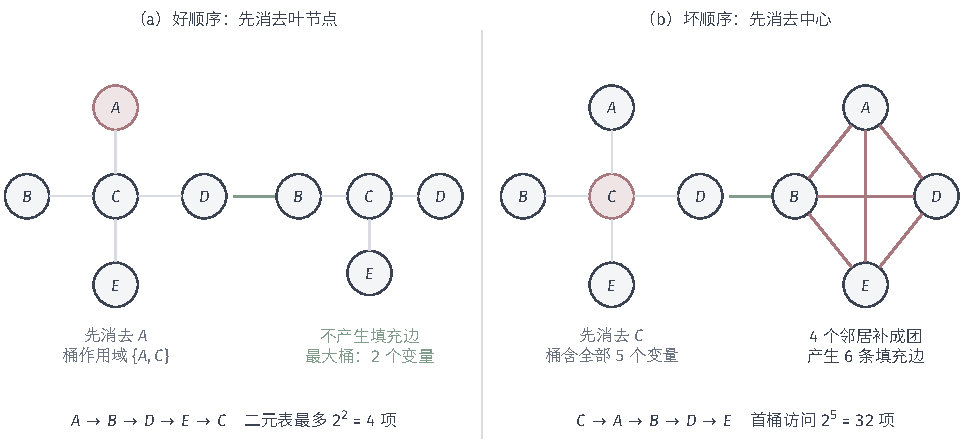
\includegraphics[width=163.153mm]{figures/06-probabilistic-graphical-models/02-inference/tikz/pgm-elimination-order-cost/figure.pdf}
  \caption{五节点二元星形图的两种消元顺序。（a）先消叶节点，每桶至多两个变量且没有填充边；（b）先消中心，首桶枚举$2^5=32$个配置，四个剩余邻居被补成团。红色节点是本步待消变量，红边是新填充边。两边比较稠密表算法的结构代价，最终数值答案保持相同。}
  \label{fig:pgm-elimination-order-cost}
\end{figure*}

在读取函数值前，可以先从作用域预测中间表。构造\term{原始关系图}（primal graph）：把每个当前因子的输入节点两两相连，以图邻接记录同一局部函数中的共同坐标。证据代入后，按剩余实际作用域建图；有向条件表的家庭先形成团，再去掉已固定坐标。这个构造保留因子输入，所得图可以异于原DAG骨架。

当前图中节点$i$的邻居记为$N(i)$。桶积使用$\{i\}\cup N(i)$，消去$i$后输出的作用域为$N(i)$，因此将这些剩余节点两两相连并删除$i$。其中新增的边称为\term{填充边}（fill edge），表示新函数的潜在共同作用域；特定参数仍可能使输出抵消或进一步分解。把该顺序产生的填充边全部保留，得到\term{诱导图}（induced graph）。

消元把内部变量的贡献保存到邻域函数。例如先消$H$，$\sum_h p(h\mid f)\ell_A(h,s)$仍以$f,s$为坐标，填充边$F-S$记录这个输出范围。对每组邻域状态，新表保存桶中子问题的完整汇总，后续直接读取它即可。图的填充说明需要保存哪些坐标，函数值说明每组坐标的数值贡献。

\begin{definition}[诱导宽度与树宽]
  \label{def:pgm-elimination-treewidth}
  对无向交互图$\mathcal{G}$的一条完整消元顺序$\pi$，令$N_t$为消去第$t$个节点之前、已经加入前面填充边后的剩余邻居集合。该顺序的\term{诱导宽度}（induced width）是
  \[
    w(\pi)=\max_t|N_t|.
  \]
  图的\term{树宽}（treewidth）定义为所有完整消元顺序中的最小诱导宽度：
  \[
    \operatorname{tw}(\mathcal{G})=\min_\pi w(\pi).
  \]
  宽度不包含本步被消去的节点，所以最大桶作用域的大小为$w(\pi)+1$。
\end{definition}

树宽给出能够达到的最小剩余邻域上界。森林可逐个消叶；含至少一条边时，其树宽为$1$。$d$节点完全图的首节点总有$d-1$个邻居，故树宽为$d-1$。这两个例子说明，节点数之外还需考虑局部作用域的重叠和可选顺序。

每个离散桶需访问多少状态，由变量基数共同决定。记$r_i=|D_i|$，定义作用域状态数
\[
  D(A)=\prod_{i\in A}r_i,\qquad D(\varnothing)=1.
\]
$D(A)$统计状态组合，集合$A$则指定变量。第$t$桶有$c_t$个因子，合并作用域$U_t=\{i_t\}\cup N_t$；稠密对齐、相乘及汇总使用$O(c_tD(U_t))$次标量操作，输出有$D(N_t)$项。完整保存乘积$\phi_t$需另有$D(U_t)$项工作存储。也可枚举每组$\bm{x}_{N_t}$，在$x_{i_t}$轴累加或取最大，把新增工作表缩至$D(N_t)$项；输入及其它未处理函数仍同时占用空间。

所有状态数至多$r$、输入因子数$m=O(d)$时，宽度$w$的完整顺序给出总运算上界
\begin{equation}
  T=O(d\,r^{w+1}).
  \label{eq:pgm-elimination-discrete-time}
\end{equation}
每个因子只在首个收集它的桶中消耗，每步再产生一个新因子，所以总处理出现次数为$O(m+d)$。去掉$m=O(d)$假设时，上式的$d$相应换为$m+d$。此处按标量运算单位成本计，精确有理数位数的增长另属位复杂度。完整物化桶积的峰值为$O(r^{w+1})$，全部新因子及MPE回溯表可由$O(d\,r^w)$上界，实际同时存活部分可能较小。总空间还包括原输入，因而需分别报告输入、临时乘积及保留输出。

边缘查询只消去$R$，保留$Q$。若显式输出完整查询联合表，最后还需$D(Q)$项。设消元阶段的最大$|N_t|$为$w_R$，无消元步骤时取$w_R=0$，将输出规模也纳入指标：
\[
  \bar w=\max\{w_R,|Q|-1,0\}.
\]
在同一基数条件下，消元与最终表乘积的总时间上界为$O((m+d)r^{\bar w+1})$，输出空间为$D(Q)$项。分析显式输出时，也可预先把$Q$补成团并安排在顺序末尾。普通树宽在全部节点的顺序中优化，此查询则要求保留$Q$，两者的候选顺序集合不同。

两种常用启发式通过当前诱导图选择下一变量。\term{最小度启发式}（min-degree）取剩余邻居最少的节点，控制当前桶的变量数；\term{最小填充启发式}（min-fill）取邻居之间缺边最少的节点，试图减少后续填充。每步补边后重新计算这些指标，才能反映当前函数作用域。局部指标可给出可用顺序，但一般不保证全局最优；最小树宽排序在一般图上是NP难问题，通常先用启发式估计中间表规模，再决定是否执行精确消元\scite{pgm-koller2009}

基数不等时，较少变量也可能组成较大表。例如三个大基数变量的桶可能超过五个二元变量的桶。\term{最小权重启发式}（min-weight）的一种约定据此比较新输出表项数，优先取$\prod_{j\in N(i)}r_j$最小的$i$，等价地比较$\sum_{j\in N(i)}\log r_j$。

若指标针对当前桶的枚举量，则比较$\sum_{j\in\{i\}\cup N(i)}\log r_j$，多计入待消变量的基数。加权填充还可对新增边$(i,j)$使用$r_ir_j$计分，它衡量新连接的成本，与前两种状态数指标不同。这些权重代理计算量，不表示概率。边缘MAP的候选还需满足阶段限制：求和完成前，先在允许求和的节点中选择。

高斯作用域的扩大增加矩阵维度及非零块。一次块消元消去$b$维、保留$a$维，对齐并累加$c_t$个稠密规范因子需$O(c_t(a+b)^2)$。式~\eqref{eq:pgm-elimination-schur}可通过分解与求解实现：Cholesky分解$\bm{J}_{B,B}$需$O(b^3)$，求解$\bm{J}_{B,B}\bm{W}=\bm{J}_{B,A}$需$O(b^2a)$，形成$\bm{J}_{A,B}\bm{W}$需$O(a^2b)$；一次项和常数更新的量级不超过这些主操作。核心更新因此使用
\begin{equation}
  T_{\mathrm{Gauss}}
  =O(b^3+b^2a+ba^2),\qquad
  S_{\mathrm{Gauss}}=O((a+b)^2).
  \label{eq:pgm-elimination-gaussian-cost}
\end{equation}
逐个消标量时$b=1$，对$a$邻居做二次规模更新，总消元典型代价为$O(\sum_t(|N_t|+1)^2)$，另计输入装配。总维度$q$的稠密高斯系统使用$O(q^3)$时间和$O(q^2)$空间，规模按矩阵维数增长。节点代表不同维度块时，成本比较需使用实际$a,b$。

\begin{table}[htbp]
  \centering
  \begin{tabularx}{\linewidth}{@{}lXX@{}}
    \toprule
    比较项 & 离散稠密表格 & 单个高斯规范形式\\
    \midrule
    作用域的表示 & 每种联合状态一项 & 二次项矩阵、一次项向量、常数\\
    合并因子 & 坐标对齐后逐项乘 & 坐标对齐后参数相加\\
    边缘消元 & 对被消去状态求和 & 配方积分与Schur补\\
    主要规模 & 基数乘积$D(U_t)$ & 矩阵块维度$a,b$\\
    填充的后果 & 新表可能指数增大 & 更多非零块与矩阵运算\\
    \bottomrule
  \end{tabularx}
  \caption{离散表与单高斯核的局部计算比较。前者以联合状态索引保存函数，后者以二次矩阵、线性向量和常数保存函数。右列的解析积分适用于单个可归一化高斯核；含离散隐变量后可能增长的混合分量另需计数。}
  \label{tab:pgm-elimination-representation-cost}
\end{table}

边缘MAP把可选顺序限制为两阶段，因而采用查询相关宽度。以$\Pi_{R\prec M}$记全部先排$R$、后排$M$的完整顺序，两组各自内部可任意排列，定义\term{受约束树宽}（constrained treewidth）为
\begin{equation}
  w_{\mathrm{c}}(\mathcal{G};R,M)
  =\min_{\pi\in\Pi_{R\prec M}}w(\pi).
  \label{eq:pgm-elimination-constrained-width}
\end{equation}
某条合法顺序的$w(\pi)$是受约束诱导宽度。候选集合是全部顺序的子集，所以最小值$w_{\mathrm{c}}\geq\operatorname{tw}(\mathcal{G})$。这个指标针对保证任意非负因子正确的两阶段稠密消元，计结构作用域成本；特定函数可交换算子的优势或其它MAP算法的时间下界属于不同分析对象。

执行一条已选合法顺序时，离散时间式~\eqref{eq:pgm-elimination-discrete-time}采用该顺序的实际宽度$w(\pi)$。采用最佳合法顺序才可用$w_{\mathrm{c}}$，得到$O((m+d)r^{w_{\mathrm{c}}+1})$上界；启发式顺序仍可能更宽。受约束树宽因此描述这组顺序可达到的最好结构上界。

以二元星形模型展示普通宽度与受约束宽度的差距。中心$X_0$连接$k$个叶$X_1,\ldots,X_k$，联合积为$p(x_0)\prod_{j=1}^k p(x_j\mid x_0)$。纯求和或MPE先消叶，每步仅一个邻居，普通树宽为$1$。若边缘MAP目标是全部叶，中心需先求和，两阶段算法的第一步为
\begin{equation}
  g(x_1,\ldots,x_k)
  =\sum_{x_0}p(x_0)\prod_{j=1}^{k}p(x_j\mid x_0).
  \label{eq:pgm-elimination-star-map}
\end{equation}
消中心后，$k$个叶成为同一函数的输入并补成团，所以受约束树宽为$k$。物化$g$需要$2^k$项，中心桶要枚举$2^{k+1}$个配置，而初始仅有$O(k)$张常数大小表。图~\ref{fig:pgm-elimination-constrained-star}显示$k=4$时的填充。

\begin{figure}[htbp]
  \centering
  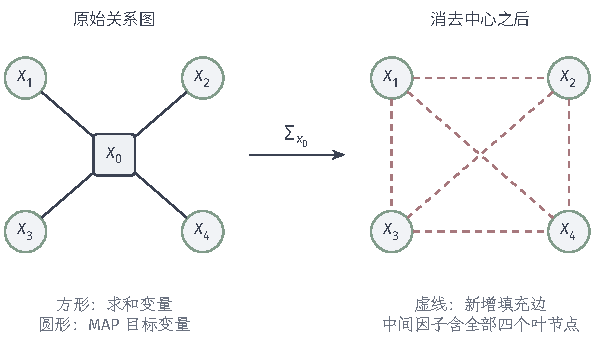
\includegraphics[width=100.651mm]{figures/06-probabilistic-graphical-models/02-inference/tikz/pgm-elimination-constrained-star/figure.pdf}
  \caption{四叶星形模型的边缘MAP消元。左图的目标是四个叶，中心$X_0$先求和；右图用虚线标出新叶间连接，记录四元输出作用域。MPE则允许先消叶，沿此顺序没有这些填充边。}
  \label{fig:pgm-elimination-constrained-star}
\end{figure}

特定参数可让式~\eqref{eq:pgm-elimination-star-map}的输出再次分解，其它算法也可利用这种结构。对仅按作用域操作的通用稠密消元，原图树宽$1$与查询受约束宽度$k$的差别却直接反映中间表增长。这解释了同一图上的边缘MAP为何可能比纯求和和MPE代价更大\scite{pgm-elimination-park2004}

\subsection{实现与适用边界}
\label{sec:pgm-elimination-implementation}

离散表的每一项需要以变量轴和状态编码定位，作用域信息随数值一起保存。相乘前按变量名对齐，或先转置再广播，可以使共享坐标确实表示同一状态。确定性约束产生的零项可用稀疏存储省去；消元后是否继续节省，则取决于新表非零项数。求和合并不同支持、填充扩大坐标范围，都可能令表变稠密，因此先估计峰值作用域，并在运行时记录非零项的实际增长。

高斯模型可用\term{稀疏Cholesky分解}（sparse Cholesky factorization）实现消元：将正定精度矩阵分解为三角因子，保存原非零项及新填充项。排序和符号分析先确定可能填充的位置，数值阶段再计算系数。相同稀疏模式可复用排序与符号结果；复用已有数值分解还要求矩阵值相同。Schur式~\eqref{eq:pgm-elimination-schur}的逆矩阵运算可用三角求解完成，$\log|\bm{J}_{B,B}|$可由分解的对角线计算。

很小的权重连续相乘时，浮点数可能下溢。\term{对数域}（log domain）保存$\log\psi$，将因子乘积改为对数相加，零权重记为$-\infty$。MPE对这些和取最大值，保留同样的回溯索引。边缘查询仍需汇总所有状态，使用对数求和指数式实现这项操作：
\begin{equation}
  \log\sum_i\exp a_i
  =a_{\max}+\log\sum_i\exp(a_i-a_{\max}),
  \qquad a_{\max}=\max_i a_i.
  \label{eq:pgm-elimination-logsumexp}
\end{equation}
当$a_{\max}$有限时，减去它后至少一个指数为$1$，其余不超过$1$，避免直接对大数取指数。全体$a_i=-\infty$表示总权重零，此时直接返回$-\infty$，绕过无定义的无穷相减。若最终查询表处处零，归一化分母也为零，程序返回证据与模型不相容。

中途缩放因子也可控制数值量级。取一个与全部因子坐标无关的$s_t>0$，将$\tau_t$保存为$\widehat{\tau}_t=\tau_t/s_t$；记累计尺度$C_t=\prod_{j=1}^t s_j$，当前不变式相应为
\[
  C_t\prod_{\psi\in\widehat{\mathcal{F}}^{(t)}}\psi
  =\text{原始函数按已执行顺序聚合后的结果}.
\]
累计尺度以$\log C_t=\sum_{j=1}^t\log s_j$保存。条件分布的公共尺度最终抵消，而证据权重及最优绝对得分需恢复它。空作用域的标量因子同样参与这个累计尺度，才能保留原权重。

高斯核的可归一化性需要说明所用空间和测度。完整精度仅半正定、却仍在整个欧氏空间使用规范形式密度时，无二次约束方向的积分会发散。模型若限定在低维仿射子空间，应明确支持及子空间测度，在该空间上积分；伪逆和伪行列式本身不足以表达这些约定。理论正定但数值接近奇异时，检查条件数、变量尺度和分解残差以判断误差放大。对角扰动可以改善数值条件，却同时改动概率模型，应在采用时说明大小及影响。

已知因子分解和明确查询后，可按预计中间作用域判断是否使用精确VE。离散表的高树宽或大受约束宽度可能耗尽内存；单高斯核按矩阵块维度增长，巨大块及填充也会带来高昂代价。相关信息无法全部保存时，第~\ref{chap:pgm-variational}章与第~\ref{chap:pgm-sampling}章分别通过变分和采样完成近似推断。

多次查询还涉及局部计算的复用。同一模型先问$F$再问$S$，从头消元会重复构造部分中间函数。模型与证据允许共享时，可缓存这些汇总，并在后续查询中读取或组合。第~\ref{chap:pgm-junction-tree}章据此组织消息与团树，减少重复工作；作用域本身很大时，其存储成本仍需承担。

\section{本章小结}
\label{sec:pgm-elimination-summary}

故障后验可以从局部因子直接计算：代入报警证据，逐桶相乘并汇总非查询状态，再统一归一化。当前乘积始终等于原函数对已消变量的聚合结果，保证局部替换和完整查询一致。报警例的$p(F=1\mid A=1)\approx0.384111$汇总全部解释，MPE的$(F,H,S)=(0,1,0)$则选择单个联合最优配置，回答不同诊断任务。

查询指定了汇总算子及输出所需信息。边缘概率累加未知状态；MPE取最大值并保存选择，逆序恢复完整配置；边缘MAP先汇总非目标状态，再选目标配置，两算子顺序一般影响答案。目标角色限制可用顺序后，受约束树宽可能大于普通树宽，星形模型也可能生成多叶联合表。

计算代价由顺序产生的作用域和所用函数表示共同决定。离散表按基数乘积保存状态组合，中间规模随诱导宽度指数增长；单高斯规范形式通过矩阵参数相加和Schur补解析更新，成本由块维度及填充决定。选择精确推断时，还需保证归一化合法，并控制浮点尺度与求解误差。中间函数可存放时，VE给出可逐步验证的查询结果；重复查询可进一步共享已有函数，过大的作用域则需要额外结构或明确的近似。

\paragraph{扩展阅读}
Koller与Friedman的教材从因子运算推导变量消除。书中不同顺序的例子可用于比较每桶的输入坐标、输出作用域及状态组合数，进一步理解中间函数为何比原节点总数更直接地决定成本\scite{pgm-koller2009}

\chapter{基于团树传播的精确推断}
\label{chap:pgm-junction-tree}

设备报警后，诊断程序先询问故障概率，随后又要计算过热概率，以及故障与传感器失灵的联合概率。对这几个查询分别运行第~\ref{chap:pgm-elimination}章的变量消除，会多次完成相同的局部求和。把这些中间表连同其依赖的因子和证据保存下来，后续查询就能接着计算。

这种按依赖关系保存的中间因子称为\term{消息}（message）。消息以边界变量的取值为输入，记录边界一侧的因子在消去内部变量后的结果。树的一条边把计算分成两侧，因而可以直接确定消息汇总的范围。对于含环的图，本章先把需要共同处理的变量组成团，再把团连成保留全部共享变量的树，随后用双向消息支持多次查询和局部证据更新。

以下以有限离散变量为对象，使用取有限非负值的因子。变量索引组成集合$V$，$X_i$的状态集合记为$\mathcal{X}_i$；$\bm{x}_A$表示索引集合$A\subseteq V$上一组变量取值。推断过程中模型参数固定，每个求和都遍历所标变量的全部状态，空乘积取$1$。

\section{从变量消除到消息传递}
\label{sec:pgm-junction-tree-from-elimination}

继续考虑设备诊断：二元变量$F,H,A,S$依次表示故障、过热、报警和传感器失灵，联合分布分解为
\begin{equation}
  p(f,h,a,s)=p(f)p(h\mid f)p(s)p(a\mid h,s).
  \label{eq:pgm-junction-tree-device}
\end{equation}
取$p(F=1)=0.1$、$p(S=1)=0.05$，以及$p(H=1\mid F=0)=0.1$、$p(H=1\mid F=1)=0.8$。表~\ref{tab:pgm-junction-tree-alarm-cpt}给出各状态下的报警概率；对应的未报警概率由$1$减去该值获得。这组人工设置的参数用于展示计算过程。

\begin{table}[htbp]
  \centering
  \begin{tabular}{ccc}
    \toprule
    $h$ & $s$ & $p(A=1\mid h,s)$\\
    \midrule
    $0$ & $0$ & $0.01$\\
    $1$ & $0$ & $0.90$\\
    $0$ & $1$ & $0.70$\\
    $1$ & $1$ & $0.99$\\
    \bottomrule
  \end{tabular}
  \caption{设备诊断例的报警条件概率。传感器正常时，过热使报警概率由$0.01$升至$0.90$；传感器失灵时，即使没有过热，报警概率也达到$0.70$。}
  \label{tab:pgm-junction-tree-alarm-cpt}
\end{table}

给定报警证据$A=1$，查询故障概率时先对传感器状态求和，形成关于$H$的表
\begin{equation}
  u(h)=\sum_s p(s)p(A=1\mid h,s),
  \qquad (u(0),u(1))=(0.0445,0.9045).
  \label{eq:pgm-junction-tree-boundary-likelihood}
\end{equation}
表$u(h)$已把传感器状态汇总完毕。保持模型参数和报警证据不变，故障查询和过热查询都可以读取这张表；它记录的是给定过热状态时报警侧的贡献。从另一侧消去故障变量，则得到
\begin{equation}
  v(h)=\sum_f p(f)p(h\mid f),
  \qquad (v(0),v(1))=(0.83,0.17).
  \label{eq:pgm-junction-tree-boundary-prior}
\end{equation}
表$v(h)$仅由故障先验和过热条件概率形成，可以在报警证据变化后继续使用。两侧通过同一个$h$组合，得到$p(h,A=1)=u(h)v(h)$。再对$h$归一化或求和，就能回答不同查询。

消息传递把中间表的变量、来源和更新方向一并记录。图~\ref{fig:pgm-junction-tree-factor-cut}给出本例的树状因子图：切断$H$与报警因子的连接后，两侧只共享$H$。给定$h$，左侧对故障求和得到$v(h)$，右侧对报警和传感器状态求和得到$u(h)$。保存整个关于$h$的函数表，使后续计算可以按所需边界状态读取；单次变量消除也可以采用这种缓存方式。

\begin{figure}[htbp]
  \centering
  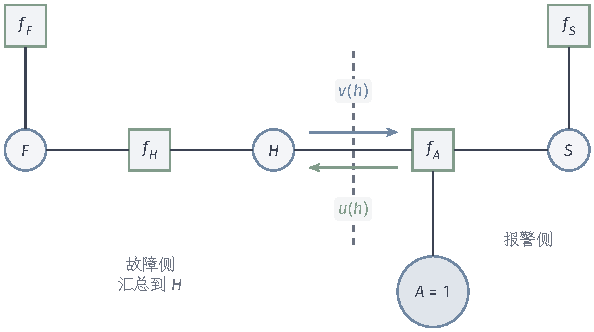
\includegraphics[width=100.651mm]{figures/06-probabilistic-graphical-models/02-inference/tikz/pgm-junction-tree-factor-cut/figure.pdf}
  \caption{设备诊断例的树状因子图。圆节点是变量，方框是因子，证据$A=1$附在报警变量处。虚线所切的两侧以$H$为共同边界，蓝色消息$v(h)$汇总故障侧，绿色消息$u(h)$汇总报警侧；箭头指示消息的发送方向。}
  \label{fig:pgm-junction-tree-factor-cut}
\end{figure}

按边界状态保存子问题结果，是动态规划在这里的具体形式。树边两侧的内部变量互不重叠，各侧的结果可以直接组合。含环图上的消息可能沿不同路径再次带回同一因子的贡献，因此需要另行处理重叠的依赖范围。

\section{树结构上的消息传递}
\label{sec:pgm-junction-tree-tree-messages}

在因子图中，因子$f_\alpha$对作用域$D_\alpha\subseteq V$中的变量进行局部计算，全部因子的索引组成$\mathcal{F}$。每个变量至少连接一个因子；孤立变量可接入恒为$1$的一元因子，以便用统一的消息形式处理。变量$i$处的证据记为$\ell_i(x_i)$：未观测时取$1$，观测$X_i=e_i$时取$\mathbf{1}\{x_i=e_i\}$。全部证据$\bm e$对应的权重和条件分布为
\begin{equation}
  \begin{aligned}
    q_{\bm{e}}(\bm{x})
      &=\prod_{\alpha\in\mathcal{F}}f_\alpha(\bm{x}_{D_\alpha})
        \prod_{i\in V}\ell_i(x_i),\\
    Z_{\bm{e}}&=\sum_{\bm{x}}q_{\bm{e}}(\bm{x}),\qquad
    p(\bm{x}\mid\bm{e})=\frac{q_{\bm{e}}(\bm{x})}{Z_{\bm{e}}}.
  \end{aligned}
  \label{eq:pgm-junction-tree-evidence-weight}
\end{equation}
当$Z_{\bm e}>0$时，归一化得到条件分布。观测变量仍留在图中，其后验质量集中在观测值上，因此证据变化时可以继续使用同一组变量和连接。对于无证据配分函数为$Z_0$的未归一化模型，硬证据概率等于$Z_{\bm e}/Z_0$；只有$Z_0=1$时才直接等于$Z_{\bm e}$。

\subsection{和积消息}
\label{sec:pgm-junction-tree-sum-product}

先设因子图连通且无环。变量$i$的相邻因子集合为$N(i)$，因子$\alpha$的相邻变量集合为$N(\alpha)=D_\alpha$。\term{和积消息}（sum-product message）将各分支的权重相乘，再对内部变量求和，留下接收方需要的变量。两类节点的更新式分别是
\begin{equation}
  m_{i\to\alpha}(x_i)
    =\ell_i(x_i)
      \prod_{\beta\in N(i)\setminus\{\alpha\}}
      m_{\beta\to i}(x_i),
  \label{eq:pgm-junction-tree-variable-message}
\end{equation}
\begin{equation}
  m_{\alpha\to i}(x_i)
    =\sum_{\bm{x}_{D_\alpha\setminus\{i\}}}
      f_\alpha(\bm{x}_{D_\alpha})
      \prod_{j\in D_\alpha\setminus\{i\}}
      m_{j\to\alpha}(x_j).
  \label{eq:pgm-junction-tree-factor-message}
\end{equation}
变量节点处的证据和入站消息都依赖同一个$x_i$，逐项相乘即可得到发出的表。因子节点则先固定接收变量$x_i$，把因子与其余变量的入站消息相乘，再遍历这些变量的状态求和。两类消息的输出都以$x_i$为索引。

乘积中排除接收方，是为了让消息只汇总发送侧。切断边$(i,\alpha)$，来自$\alpha$的消息汇总另一侧，乘入它就会重复计数。因子发送消息时，删除$\alpha$使其余邻接变量分属互不重叠的分支；给定这些变量的状态，各分支先独立求和。将结果与$f_\alpha$相乘，再消去接收变量以外的变量，便得到式~\eqref{eq:pgm-junction-tree-factor-message}。

把本例的四个因子写成$f_F=p(f)$、$f_H=p(h\mid f)$、$f_S=p(s)$、$f_A=p(a\mid h,s)$。从叶端开始，故障和传感器变量分别发送$m_{F\to f_H}(f)=p(f)$、$m_{S\to f_A}(s)=p(s)$；报警变量发送证据表$m_{A\to f_A}(a)=\mathbf{1}\{a=1\}$。两个相邻因子随后向$H$发送
\[
  \begin{aligned}
    m_{f_H\to H}(h)&=\sum_f p(h\mid f)p(f)=v(h),\\
    m_{f_A\to H}(h)&=\sum_{a,s}p(a\mid h,s)
       \mathbf{1}\{a=1\}p(s)=u(h).
  \end{aligned}
\]
$H$处没有额外证据，因此发往报警因子的消息为$m_{H\to f_A}=v$，发往故障因子的消息为$m_{H\to f_H}=u$。同一条边的两个方向分别携带两侧的汇总结果，各自具有不同的因子来源。树上的许多动态规划都可写成这样的局部和积运算\scite{pgm-overview-kschischang2001}

\subsection{消息调度与边缘恢复}
\label{sec:pgm-junction-tree-scheduling}

每次发送前，节点先等待除接收方之外的全部入站消息。选一个变量节点为根，从叶端向根进行\term{收集}（collect）：叶变量发送$\ell_i$，叶因子发送自身的一元函数，其余节点在分支结果到齐后继续向上发送。根收到各侧贡献后，再向叶端进行\term{分发}（distribute），使每个节点都能收到来自父侧的贡献。

有$M$条边的因子树共计算$2M$条有向消息，每条边的两个方向各一次。收集按叶到根的依赖顺序完成，分发再按根到叶的顺序完成，这两轮计算就能结束。根的边缘只需收集结果；查询其他位置的边缘时，分发提供它们所缺的另一侧信息。

把全部入站消息与节点处的局部输入组合，得到
\begin{equation}
  \begin{aligned}
    B_i(x_i)&=\ell_i(x_i)\prod_{\alpha\in N(i)}
       m_{\alpha\to i}(x_i),\\
    B_\alpha(\bm{x}_{D_\alpha})
      &=f_\alpha(\bm{x}_{D_\alpha})
        \prod_{j\in D_\alpha}m_{j\to\alpha}(x_j).
  \end{aligned}
  \label{eq:pgm-junction-tree-factor-beliefs}
\end{equation}
围绕$i$或$\alpha$切开树，各分支汇总其余因子，因而$B_i=\sum_{\bm{x}_{V\setminus\{i\}}}q_{\bm e}$、$B_\alpha=\sum_{\bm{x}_{V\setminus D_\alpha}}q_{\bm e}$。除以$Z_{\bm e}$，两者就是相应的后验边缘。若$i,j\in D_\alpha$，还可对$B_\alpha$的其余变量求和，得到$p(x_i,x_j\mid\bm e)$。成对因子的作用域正好覆盖原变量交互图的一条边；在二部因子图中，这两个变量通过同一个因子节点相连。

报警例的$H$处给出
\begin{equation}
  (B_H(0),B_H(1))=(0.036935,0.153765),
  \qquad Z_{\bm{e}}=0.19070.
  \label{eq:pgm-junction-tree-alarm-normalizer}
\end{equation}
据此得到$p(H=1\mid A=1)\approx0.806319$。向故障侧分发时，先计算$m_{f_H\to F}(f)=\sum_h p(h\mid f)u(h)=(0.1305,0.7325)$，再乘故障先验。故障状态$F=1$的权重为$0.07325$，归一化得到$p(F=1\mid A=1)=0.07325/0.19070\approx0.384111$。

这些数值保留了消息的原始尺度。为降低连乘下溢的风险，可以将非零消息整体除以正数；最终将局部汇总表归一化，后验边缘保持不变。此时$B_i$的总和带有消息缩放后的尺度，计算证据概率还需要保存并恢复缩放常数。全零消息表示发送侧在所有边界状态下都没有与证据相容的正权重配置，应保留这项零权重信息。

\subsection{最大积消息}
\label{sec:pgm-junction-tree-max-product}

寻找完整状态的最优解释时，要比较各配置的权重，而非累加它们。\term{最大积消息}（max-product message）以边界状态为索引，保存一侧子树能取得的最大权重。用$\nu$表示这套消息，将和积公式中的求和换成最大化，得到
\begin{equation}
  \begin{aligned}
    \nu_{i\to\alpha}(x_i)
      &=\ell_i(x_i)\prod_{\beta\in N(i)\setminus\{\alpha\}}
         \nu_{\beta\to i}(x_i),\\
    \nu_{\alpha\to i}(x_i)
      &=\max_{\bm{x}_{D_\alpha\setminus\{i\}}}
         f_\alpha(\bm{x}_{D_\alpha})
         \prod_{j\in D_\alpha\setminus\{i\}}
         \nu_{j\to\alpha}(x_j).
  \end{aligned}
  \label{eq:pgm-junction-tree-factor-max}
\end{equation}
由于分支变量互不重叠且因子非负，$\max_{\bm y,\bm z}g(\bm y)h(\bm z)=(\max_{\bm y}g)(\max_{\bm z}h)$，各侧最优值可以相乘。为了恢复最优配置，计算$\nu_{\alpha\to i}(x_i)$时，同时保存一组达到最大值的$\bm{x}_{D_\alpha\setminus\{i\}}$。这张从边界状态查找内部最优选择的表称为\term{回溯记录}（backpointer）。

将最大积入站消息全部组合，形成$\widehat{B}_i(x_i)=\ell_i(x_i)\prod_{\alpha\in N(i)}\nu_{\alpha\to i}(x_i)$。它记录固定$x_i$时全图的最大权重，称为\term{最大边缘}（max-marginal）。同一边界状态下，最大边缘取一组最优配置的权重，概率边缘则累加全部配置的权重。

收集后先在根处选择使证据与入站消息乘积最大的状态，再逐层读取回溯表：父变量状态确定后，查出相邻因子其余变量的状态，继续进入各分支。出现平局时，按固定顺序记录其中一组选择，回溯保持这组条件选择的关联。例如两个二元变量仅在$(0,0)$和$(1,1)$上权重为$1$，其余权重为零；两处最大边缘都对$0,1$平局，独立选择可能得到零权重的$(0,1)$。沿回溯记录选择，才能取得一组相容的最优解。

在设备诊断例中，以$H$为根，故障侧发送的最大权重为
\[
  \begin{aligned}
    \nu_{f_H\to H}(0)&=\max(0.9\times0.9,\;0.1\times0.2)=0.81,\\
    \nu_{f_H\to H}(1)&=\max(0.9\times0.1,\;0.1\times0.8)=0.09.
  \end{aligned}
\]
这两个$h$状态的回溯表都选$f=0$。报警侧在$h=0$时比较$0.95\times0.01$和$0.05\times0.70$，选$s=1$，权重为$0.035$；在$h=1$时比较$0.95\times0.90$和$0.05\times0.99$，选$s=0$，权重为$0.855$。根处的两个候选值为$0.02835$和$0.07695$，分别来自$0.81\times0.035$和$0.09\times0.855$，因此选$h=1$。回溯得到MPE配置$(f,h,s)=(0,1,0)$，未归一化权重为$0.07695$；报警变量保持证据值$A=1$。式~\eqref{eq:pgm-junction-tree-boundary-prior}和式~\eqref{eq:pgm-junction-tree-boundary-likelihood}中的和积表汇总全部配置，需与这套最大积表分别保存。

对于隐状态链，记状态为$Z_t$、观测为$X_t=x_t$。最大积收集依次向时间后端汇总，写成
\[
  \delta_t(z_t)=p(x_t\mid z_t)
    \max_{z_{t-1}}\{\delta_{t-1}(z_{t-1})p(z_t\mid z_{t-1})\}.
\]
从$\delta_1(z_1)=p(z_1)p(x_1\mid z_1)$开始，为每个$z_t$保存最优前驱状态，再由末端向前回溯，就得到Viterbi动态规划。它求解全部隐状态的联合最优配置，第~\ref{sec:pgm-dynamic-discrete}节将用于离散时序模型。若查询仅最大化部分变量，其余变量仍须求和，应采用第~\ref{sec:pgm-elimination-map}节的边缘MAP顺序。

\section{团树的构造}
\label{sec:pgm-junction-tree-construction}

含环因子图的两侧可能共享多个变量。将这些变量共同保留在消息中，便可以把一片局部计算组合成新的节点。\term{团树}（junction tree）的节点就是这样的变量团，边上的分隔集记录相邻团共享的变量。一个变量可能出现在多个团中，树上连接这些团的整条路径都须保留它，才能按同一个状态组合各处的因子。

图~\ref{fig:pgm-junction-tree-triangulation}以四环说明构造过程。消元产生的共同作用域先由填充边记录，随后用极大团容纳这些变量。将极大团连接起来，以交集为消息边界，再为原始因子选择存放位置，即可沿树边汇总两侧贡献。填充边和团节点用于组织计算，原联合分布仍由原始因子的乘积给出。

\begin{figure*}[htbp]
  \centering
  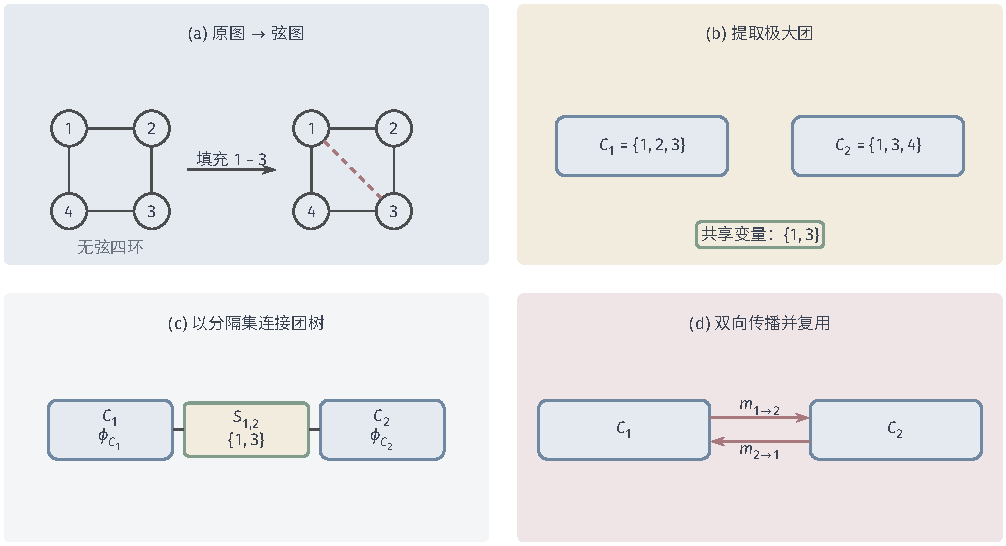
\includegraphics[width=169.000mm]{figures/06-probabilistic-graphical-models/02-inference/tikz/pgm-junction-tree-triangulation/figure.pdf}
  \caption{四环模型的团树构造与传播。添加填充边$1-3$后，两个极大团为$C_1=\{1,2,3\}$、$C_2=\{1,3,4\}$，共享变量组成分隔集$S_{1,2}=\{1,3\}$。最后一个面板在团间保存双向消息，用分隔集的状态组合两侧计算结果。}
  \label{fig:pgm-junction-tree-triangulation}
\end{figure*}

\subsection{从原图到弦图}
\label{sec:pgm-junction-tree-chordalization}

每个原始因子的全部变量需要放在同一个团内。有向模型的因子$p(x_i\mid\bm{x}_{\operatorname{pa}(i)})$涉及$i$及其父节点，因此先把共同子节点的父节点相连，再去掉方向，形成承载全部因子的道德图。这里保留全部变量，而条件独立检验会按具体查询选取祖先子图。在报警例中，两个报警父节点$H,S$由此相连，形成团$\{F,H\}$和$\{H,A,S\}$。

无向模型直接使用承载因子作用域的变量图；因子图则先将每个作用域中的变量两两相连。选定消元顺序后，每次把当前节点的剩余邻居全部相连，再移去该节点。将新增边保留在原变量集合上，得到\term{三角化}（triangulation）或弦化后的图；其中长度至少为$4$的环都有弦。

第~\ref{sec:pgm-elimination-complexity}节的最小度和最小填充启发式分别按剩余邻居数和缺失邻居边数选节点。填充记录消元后新因子的共同变量，每一步的求和仍完整保留被消变量的贡献。合法顺序给出相同的概率答案，但中间表和后续消息的规模可能不同。

完成填充后，所选顺序中每个节点的剩余邻居都两两相连，所以该顺序是完美消元序，所得图为弦图（参见\BookTheoremRef{thm:graph-theory-chordal-perfect-elimination}{卷1《数学准备：计算、分析与几何》第9章“图的表示与计算”第9.3.2.3节“弦图条件下的无填充分解”}）。

填充保留消元需要的共同作用域，数值计算继续使用原因子和原参数。

对四环$1-2-3-4-1$，先消去$2$会添加$1-3$，形成极大团$\{1,2,3\}$、$\{1,3,4\}$；先消去$1$则添加$2-4$，形成$\{1,2,4\}$、$\{2,3,4\}$，如图~\ref{fig:pgm-junction-tree-triangulation}所示。两种计算都保留原分布，消息的索引却分别为$\{1,3\}$和$\{2,4\}$。这两个变量组的状态数决定了不同的消息表成本。

\subsection{极大团、分隔集与运行交集性质}
\label{sec:pgm-junction-tree-running-intersection}

团中的变量两两相连。\term{极大团}（maximal clique）指已无法加入其他节点的团；它可以小于全图节点数最多的团。记全部极大团为$\mathcal C$，以它们为节点构造树$\mathcal T=(\mathcal C,\mathcal E_{\mathcal T})$。相邻团$C,D$的交集$S_{C,D}=C\cap D$称为\term{分隔集}（separator），消息以其中变量的共同取值为索引。

图~\ref{fig:pgm-junction-tree-running-intersection}上排把$\{1,2\}$、$\{2,3\}$、$\{3,4\}$依次连接。含$2$的两团相邻，含$3$的两团也相邻，$1,4$各只出现在一团中。下排把$\{3,4\}$移到中间，连接含$2$的两团时就需要经过一个不含$2$的团，消息无法在这条路径上保留$x_2$。

共享变量需要沿整条团间路径传递。若路径中途删去$i$，另一端的因子仍需与发送端按同一个$x_i$组合，而传到那里时已经没有这个索引。因此对团的连接还要施加以下条件。

\begin{definition}[运行交集性质]
  \label{def:pgm-junction-tree-running-intersection}
  团树满足\term{运行交集性质}（running intersection property），是指对任意变量$i$，包含$i$的全部团构成连通子树。等价地，对任意两个团$C,D$，从$C$到$D$的唯一路径上的每个团都包含$C\cap D$。
\end{definition}

树中任意两团之间只有一条路径。包含$i$的团若构成连通子树，这条路径上的团都含$i$；反过来，若任意两处之间的路径都保留$i$，含$i$的团就相互连通。

\begin{figure}[htbp]
  \centering
  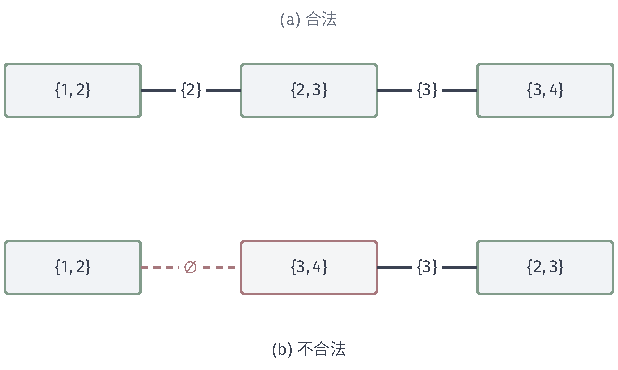
\includegraphics[width=104.652mm]{figures/06-probabilistic-graphical-models/02-inference/tikz/pgm-junction-tree-running-intersection/figure.pdf}
  \caption{运行交集性质的两种连接示例。上排每个变量出现的团都连续相连；下排连接含$2$的两团时，中间团$\{3,4\}$缺少$2$，沿该路径计算的消息会丢失共同状态$x_2$。}
  \label{fig:pgm-junction-tree-running-intersection}
\end{figure}

运行交集确定了每条消息需要保留的完整边界。删除边$(C,D)$，记$C$侧的团集合为$\mathcal C_{C\mid D}$，其中所有变量的并集为$U_{C\mid D}=\bigcup_{K\in\mathcal C_{C\mid D}}K$，则两侧的共同变量满足
\begin{equation}
  U_{C\mid D}\cap U_{D\mid C}=S_{C,D}.
  \label{eq:pgm-junction-tree-cut-intersection}
\end{equation}
$S_{C,D}$中的变量属于边的两端，所以一定出现在两侧。反之，若$i$在两侧的某个团中各出现一次，连接这两个团的路径经过$(C,D)$，运行交集迫使$C,D$都含$i$。因此两侧交集恰为$S_{C,D}$，消息可以消去其余内部变量。

给定分隔集状态，两侧便可各自求和，再相乘，这正是团树动态规划的分解方式。分配律和完整的边界保证结果精确；稠密离散表的成本仍指数依赖所选顺序的诱导宽度。实际计算需要团的状态空间足够小，能够存储并遍历这些表。

遗漏共享变量会改变求和结果。为二元链的三个团依次分配$\mathbf{1}\{x_1=x_2\}$、$\mathbf{1}\{x_2=x_3\}$、$\mathbf{1}\{x_3=x_4\}$，全局仅全$0$和全$1$的配置有非零权重，权重总和为$2$。若使用下排的错误连接，并以$\{1,2\}$为根，$\{2,3\}$先向$\{3,4\}$发送常数$1$，后者再经空分隔集向根发送标量$2$。根的求和得到$2\times2=4$：本应共享的$x_2$被分别消去，使两个局部求和组合了彼此不相容的状态。

\subsection{团树构造与因子分配}
\label{sec:pgm-junction-tree-spanning-tree}

弦图的极大团可以通过\term{团交图}（clique intersection graph）选择连接：以极大团为节点，将两团的交集大小
\[
  w(C,D)=|C\cap D|
\]
用作边权。非空交集产生正权边；对于不连通的原图，可用零权边连接不同分量，此时消息只携带空分隔集上的标量。以下把零权边也加入候选，以统一处理各连通分量。

对于非空有限弦图，把全部极大团作为节点，以交集大小为边权构成完全团图，其中保留交集为空的零权边。满足运行交集的生成树，恰好是总交集权最大的生成树（参见\BookTheoremRef{thm:graph-theory-clique-tree-maximum-weight}{卷1《数学准备：计算、分析与几何》第9章“图的表示与计算”第9.3.2.3节“弦图条件下的无填充分解”}）。选好团间连接后，还要为团分配概率因子，计算消息和边缘。

可以用最大权Kruskal算法选边。将候选边按权重从大到小排列，平局按固定顺序处理；从空边集开始，只有两端尚未连通时才加入当前边，以保持无环。选出$|\mathcal C|-1$条边、使全部团连通后，即得到所需的最大权生成树。

对于图~\ref{fig:pgm-junction-tree-running-intersection}中的三个团，$\{1,2\}$与$\{2,3\}$共享$2$，$\{2,3\}$与$\{3,4\}$共享$3$，首尾两团交集为空。候选边权为$1,1,0$，先加入的两条正权边已经形成上排的链。余下的零权边连接已连通的两端，会形成环，因此跳过。

定理适用于已完成三角化的弦图。四环的四个边团就无法组成运行交集树，选最大权生成树也会丢失某个共享变量。三角化先决定极大团的规模，最大权选边随后保证同一变量所在的团连续相连；这一步并不优化先前的消元顺序。图模型教材进一步讨论了分解图、团树与局部计算的关系\scite{pgm-lauritzen1996}

确定树以后，将每个原始因子$f_\alpha$存入一个覆盖其全部变量的团$a(\alpha)$，即$D_\alpha\subseteq a(\alpha)$。每个因子恰好分配一次，从而得到无证据团势
\begin{equation}
  \phi_C^0(\bm{x}_C)
    =\prod_{\alpha:\,a(\alpha)=C}f_\alpha(\bm{x}_{D_\alpha}),
  \qquad
  \prod_{C\in\mathcal{C}}\phi_C^0
    =\prod_{\alpha\in\mathcal{F}}f_\alpha.
  \label{eq:pgm-junction-tree-factor-assignment}
\end{equation}
未分到因子的团取势$1$。一个因子即使被多个团覆盖，也只存放一份，否则重复乘入会改变原乘积。报警例中取$C_1=\{F,H\}$、$C_2=\{H,A,S\}$，分别存放$\phi_{C_1}^0=p(f)p(h\mid f)$、$\phi_{C_2}^0=p(s)p(a\mid h,s)$，两团通过$H$组合。

合法的分配位置、最大权树和三角化可能有多种选择，它们都保留原始因子乘积，却形成不同的局部表和缓存依赖。选择时需同时考虑消息复用和表格规模：即使团树只有很少节点，一个大团也可能需要难以容纳的状态表。

\section{团树传播}
\label{sec:pgm-junction-tree-propagation}

运行交集已经确定两团之间的完整边界。下面沿这些边界进行数值计算，将因子树上的单变量消息推广为多变量表。本节分别保存每条边的双向消息，每次从局部输入和其他入站消息重新形成输出；公式只含乘法与求和，可以保留因子和证据中的零表项。

\subsection{团势与团间消息}
\label{sec:pgm-junction-tree-clique-messages}

\term{团势}（clique potential）保存分配给该团的原始因子及证据，取值非负，通常尚未归一化。它是局部计算的输入，传播完成后的边缘还需汇合全树的消息。为变量证据$\ell_i$选择一个含$i$的团$h(i)$，定义
\begin{equation}
  \phi_C(\bm{x}_C)=\phi_C^0(\bm{x}_C)
    \prod_{i:\,h(i)=C}\ell_i(x_i).
  \label{eq:pgm-junction-tree-local-evidence}
\end{equation}
每个原始因子和证据都恰好出现一次，因此$\prod_C\phi_C=q_{\bm e}$。多变量观测似然也可按相同方式吸收，但需由一个团覆盖全部作用域，并给出该似然的观测含义。一般软证据重复分配会重复乘入其权重，改变目标分布。

记团$C$的邻居集合为$N_{\mathcal T}(C)$。图~\ref{fig:pgm-junction-tree-message}展示发送$C\to D$的步骤：将$\phi_C$与除$D$之外的入站消息相乘，再对$C\setminus S_{C,D}$求和，留下分隔集上的表。反向消息按同一公式汇总$D$侧；两条消息一起提供共享变量两侧的完整贡献。

\begin{figure*}[htbp]
  \centering
  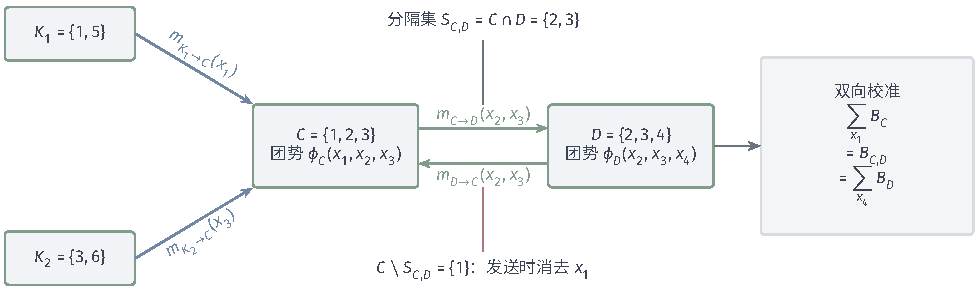
\includegraphics[width=165.650mm]{figures/06-probabilistic-graphical-models/02-inference/tikz/pgm-junction-tree-message/figure.pdf}
  \caption{团间消息与共享变量的汇总。蓝色入站消息与$\phi_C$相乘后，消去$C\setminus S_{C,D}=\{1\}$，得到以$\{2,3\}$为索引的$m_{C\to D}$；$D$侧消息留待后续组合。右侧两个方向的绿色消息共同形成$B_{C,D}$，校准后相邻团分别消去非共享变量，也得到这张分隔集表。}
  \label{fig:pgm-junction-tree-message}
\end{figure*}

对应的消息公式为
\begin{equation}
  m_{C\to D}(\bm{x}_{S_{C,D}})
    =\sum_{\bm{x}_{C\setminus S_{C,D}}}
      \phi_C(\bm{x}_C)
      \prod_{K\in N_{\mathcal{T}}(C)\setminus\{D\}}
        m_{K\to C}(\bm{x}_{S_{K,C}}).
  \label{eq:pgm-junction-tree-clique-message}
\end{equation}
计算乘积时，各函数按共同变量的状态对齐，较小作用域的函数在其余坐标上重复取值。局部势$\phi_C$保留原来的输入；新的消息另行保存，供其他方向的发送和后续查询使用。

将局部势与全部入站消息组合，并将一条边的两个方向消息组合，分别定义
\begin{equation}
  \begin{aligned}
    B_C(\bm{x}_C)
      &=\phi_C(\bm{x}_C)
        \prod_{K\in N_{\mathcal{T}}(C)}
          m_{K\to C}(\bm{x}_{S_{K,C}}),\\
    B_{C,D}(\bm{x}_{S_{C,D}})
      &=m_{C\to D}(\bm{x}_{S_{C,D}})
        m_{D\to C}(\bm{x}_{S_{C,D}}).
  \end{aligned}
  \label{eq:pgm-junction-tree-clique-separator-beliefs}
\end{equation}
传播完成后，$B_C$作为团的汇总势，包含全树对该团状态的贡献。边上的\term{分隔集势}（separator potential）$B_{C,D}$由两侧消息相乘形成，用于读取共同变量的权重。它是传播结果，原模型仍由局部团势的乘积定义。不同边即使交集相同，也各自保存双向消息和分隔集表。

把报警指示函数$\ell_A(a)=\mathbf{1}\{a=1\}$存入$C_2$，本例的局部势为
\[
  \begin{aligned}
    \phi_{C_1}(f,h)&=p(f)p(h\mid f),\\
    \phi_{C_2}(h,a,s)&=p(s)p(a\mid h,s)\ell_A(a).
  \end{aligned}
\]
每团都只有一个邻居，因此发往对方的消息直接对自身局部势求和：
\begin{equation}
  \begin{aligned}
    m_{C_1\to C_2}(h)&=\sum_f p(f)p(h\mid f)=v(h),\\
    m_{C_2\to C_1}(h)&=\sum_{a,s}p(s)p(a\mid h,s)\ell_A(a)=u(h).
  \end{aligned}
  \label{eq:pgm-junction-tree-device-clique-messages}
\end{equation}
两张表仍是前面得到的$v(h)$和$u(h)$。团树把多步局部消元合并到一次团间发送中，使用的数值运算仍是因子乘法和内部变量求和。

\subsection{收集、分发与校准}
\label{sec:pgm-junction-tree-calibration}

选团$R$为根后，先从叶团向上收集；非叶团等所有子团消息到齐，再向父团发送。根取得全部入站消息后，向各子团分发，逐层传下根侧的贡献。算法~\ref{alg:pgm-junction-tree-calibrate}按后序和先序遍历实现这两轮调度；尚未收到的消息需要等待计算，空邻居集合的乘积则取$1$。

\begin{algorithm}[团树上的和积校准]
  \label{alg:pgm-junction-tree-calibrate}
  \begin{algorithmic}[1]
    \Require 满足运行交集的团树、局部势$\{\phi_C\}$、根$R$
    \Ensure 全部双向消息、汇总势$\{B_C,B_{C,D}\}$和$Z_{\bm{e}}$
    \State 将树定根，记录每个非根团的父团
    \For{按后序遍历访问的非根团$C$}
      \State 按式~\eqref{eq:pgm-junction-tree-clique-message}发送$C$到父团的消息
    \EndFor
    \For{按先序遍历访问的团$C$}
      \For{$C$的每个子团$D$}
        \State 按式~\eqref{eq:pgm-junction-tree-clique-message}发送$C\to D$
      \EndFor
    \EndFor
    \State 按式~\eqref{eq:pgm-junction-tree-clique-separator-beliefs}形成汇总势
    \State 计算$Z_{\bm{e}}=\sum_{\bm{x}_R}B_R(\bm{x}_R)$
    \If{$Z_{\bm{e}}=0$}
      \State 报告证据与模型不相容，不输出条件概率
    \Else
      \State 令$b_C=B_C/Z_{\bm{e}}$、$b_{C,D}=B_{C,D}/Z_{\bm{e}}$
    \EndIf
  \end{algorithmic}
\end{algorithm}

双向传播后，相邻团对同一分隔集给出一致的边缘。这种重叠边缘的一致性称为\term{校准}（calibration）：各团消去非共享变量，得到同一张分隔集表。图~\ref{fig:pgm-junction-tree-message}右侧显示了这个条件；这里的校准涉及概率表之间的一致性，与分类置信度的经验校准含义不同。

对边$(C,D)$，从$C$的汇总势消去$C\setminus S_{C,D}$。入站消息$m_{D\to C}$仅依赖分隔集，能够提出求和号，于是
\begin{equation}
  \begin{aligned}
    &\sum_{\bm{x}_{C\setminus S_{C,D}}}B_C(\bm{x}_C)\\
      &\quad=m_{D\to C}
        \sum_{\bm{x}_{C\setminus S_{C,D}}}
          \phi_C\prod_{K\in N_{\mathcal{T}}(C)\setminus\{D\}}m_{K\to C}\\
      &\quad=m_{D\to C}m_{C\to D}=B_{C,D}.
  \end{aligned}
  \label{eq:pgm-junction-tree-local-calibration}
\end{equation}
从$D$侧求和也得到两条消息的乘积$B_{C,D}$，所以共享变量的汇总一致。第~\ref{sec:pgm-junction-tree-correctness}节还会把消息与原始因子的全局求和联系起来，说明这些一致的表正是输入模型的边缘。

表~\ref{tab:pgm-junction-tree-calibrated-separator}列出报警例的双向消息。固定每行的$h$，乘积给出$H=h$且发生报警的权重；最后一列的总和$0.19070$为报警概率。

\begin{table}[htbp]
  \centering
  \begin{tabular}{cccc}
    \toprule
    $h$ & $m_{C_1\to C_2}(h)$ & $m_{C_2\to C_1}(h)$ & $B_{C_1,C_2}(h)$\\
    \midrule
    $0$ & $0.83$ & $0.0445$ & $0.036935$\\
    $1$ & $0.17$ & $0.9045$ & $0.153765$\\
    \bottomrule
  \end{tabular}
  \caption{报警例的消息与分隔集权重。两条消息分别汇总故障侧和报警侧，乘积给出$p(h,A=1)$；将末列归一化便得到过热后验。}
  \label{tab:pgm-junction-tree-calibrated-separator}
\end{table}

两个团的完整汇总表如下。第一张以$f$为行、$h$为列，第二张以$h$为行、$s$为列，并只列出$a=1$切片；证据将$a=0$切片置零。
\begin{equation}
  \begin{aligned}
    \bigl[B_{C_1}(f,h)\bigr]_{f,h}
      &=\begin{pmatrix}
          0.036045&0.081405\\
          0.000890&0.072360
        \end{pmatrix},\\
    \bigl[B_{C_2}(h,1,s)\bigr]_{h,s}
      &=\begin{pmatrix}
          0.007885&0.029050\\
          0.145350&0.008415
        \end{pmatrix}.
  \end{aligned}
  \label{eq:pgm-junction-tree-device-calibrated-tables}
\end{equation}
第一张矩阵沿$f$求和，第二张沿$s$求和，都得到$(0.036935,0.153765)$，两者的总和也同为$0.19070$。这两个方向的边缘化直接显示了团表在$H$上的一致性，也核对了本例的因子分配和消息计算。

消息若分别缩放，团汇总表也会带有各自的尺度。先归一化各团表，再比较分隔集上的概率边缘，即可检查一致性。通过局部表示吸收证据并沿连接传播，是经典精确图模型推断的方法\scite{pgm-overview-lauritzen1988}

\subsection{查询与证据更新}
\label{sec:pgm-junction-tree-queries-updates}

校准后的团表已经汇总全部证据。若查询集合$Q$由团$C$覆盖，对其余团内变量求和就得到
\begin{equation}
  p(\bm{x}_Q\mid\bm{e})
    =\sum_{\bm{x}_{C\setminus Q}}b_C(\bm{x}_C).
  \label{eq:pgm-junction-tree-covered-query}
\end{equation}
这一步复用现有消息，只计算团内的边缘化及输出表。报警例的$F,H$在$C_1$中，$H,S$在$C_2$中；相应地消去$H$，得到$p(F=1\mid A=1)\approx0.384111$和$p(S=1\mid A=1)\approx0.196460$。

查询$\{F,S\}$需要结合两个团。两团的汇总势各自包含全图贡献，直接相乘会再次计入共同的$H$权重。将这份重复权重除去，再消去$H$，本例得到
\begin{equation}
  p(f,s\mid A=1)
    =\frac{1}{Z_{\bm{e}}}
      \sum_h
       \frac{B_{C_1}(f,h)B_{C_2}(h,1,s)}
            {B_{C_1,C_2}(h)}.
  \label{eq:pgm-junction-tree-cross-clique-device}
\end{equation}
本例两种$h$状态的分母都为正。固定$(f,s)=(0,0)$，归一化前的两个$h$项为
\[
  \begin{aligned}
    &\frac{0.036045\times0.007885}{0.036935}
     +\frac{0.081405\times0.145350}{0.153765}\\
    &=0.007695+0.076950=0.084645.
  \end{aligned}
\]
除以分隔集势以后，每个$h$状态的共同贡献只保留一份。表~\ref{tab:pgm-junction-tree-cross-query}给出四组$(f,s)$的结果，与直接消去$H$的联合表一致。

\begin{table}[htbp]
  \centering
  \begin{tabular}{cccc}
    \toprule
    $f$ & $s$ & $p(f,s,A=1)$ & $p(f,s\mid A=1)$\\
    \midrule
    $0$ & $0$ & $0.084645$ & $0.443865$\\
    $0$ & $1$ & $0.032805$ & $0.172024$\\
    $1$ & $0$ & $0.068590$ & $0.359675$\\
    $1$ & $1$ & $0.004660$ & $0.024436$\\
    \bottomrule
  \end{tabular}
  \caption{跨团查询$(F,S)$的联合权重与后验。先按分隔集$H$组合两团的汇总表，再消去$H$；末列保留六位小数，显示两个查询变量在报警证据下的联合分布。}
  \label{tab:pgm-junction-tree-cross-query}
\end{table}

重复的分隔集权重随$h$变化，因此会改变相对概率。直接把两团表相乘再求和，将得到
\[
  \widetilde{q}(f,s)=\sum_h B_{C_1}(f,h)B_{C_2}(h,1,s).
\]
对这个$\widetilde q$归一化后，故障概率约为$0.446232$，偏离正确的$0.384111$。多乘的$B_{C_1,C_2}(h)$改变了两种$h$状态的相对权重，整体归一化只能消去常数尺度。

一般跨团查询可以保留连接查询变量的团子树。先为每个查询变量选一个包含它的团，将连接这些团的子树节点记为$\mathcal H\subseteq\mathcal C$，所有相关变量的并集记为$W=\bigcup_{C\in\mathcal H}C$。把树外分支的既有消息吸收到子树局部势，计算
\begin{equation}
  \begin{aligned}
    \widetilde{\phi}_C
      &=\phi_C
        \prod_{D\in N_{\mathcal{T}}(C)\setminus\mathcal{H}}m_{D\to C},\\
    g_Q(\bm{x}_Q)
      &=\sum_{\bm{x}_{W\setminus Q}}
         \prod_{C\in\mathcal{H}}\widetilde{\phi}_C(\bm{x}_C),\\
    p(\bm{x}_Q\mid\bm{e})&=g_Q(\bm{x}_Q)/Z_{\bm{e}}.
  \end{aligned}
  \label{eq:pgm-junction-tree-subtree-query}
\end{equation}
运行交集使每个外部分支只经自己的分隔集连接这棵子树，入站消息已完成对$V\setminus W$的求和。随后在子树内部消元，即可得到$g_Q$；可以逐步计算中间表，避免直接展开整个$W$联合表。这一表达只用乘法和求和，也适用于零表项。

若只保存校准后的团边缘与分隔集边缘，则可在分隔集概率为正的状态上重构
\begin{equation}
  p(\bm{x}_W\mid\bm{e})
    =\frac{\prod_{C\in\mathcal{H}}b_C(\bm{x}_C)}
           {\prod_{(C,D)\in\mathcal{E}_{\mathcal{H}}}
                b_{C,D}(\bm{x}_{S_{C,D}})},
  \label{eq:pgm-junction-tree-calibrated-factorization}
\end{equation}
其中$\mathcal E_{\mathcal H}$为子树的内部边集，再消去$W\setminus Q$便得到查询结果。代入式~\eqref{eq:pgm-junction-tree-clique-separator-beliefs}，每条内部边的两个方向消息各约去一次，剩下$\prod_C\widetilde\phi_C$。树的节点数比边数多一，归一化因子也相应剩下$1/Z_{\bm e}$，得到与式~\eqref{eq:pgm-junction-tree-subtree-query}相同的结果。

分隔集概率为零时，所有与该状态一致的完整配置概率也为零。可直接用无除法的式~\eqref{eq:pgm-junction-tree-subtree-query}计算；也可对子树定根，仅在正概率的父分隔集状态上用$b_C/b_{C,D}$形成条件表，其余分支整体赋零。这样可为式~\eqref{eq:pgm-junction-tree-calibrated-factorization}在零概率状态上补零。查询少量边缘时可继续局部消元，而大规模联合表还需要支付写出全部表项的成本。

查询一组MPE时，另行计算最大积消息$\nu_{C\to D}$。消息内部使用最大化，并为每个分隔集状态保存内部最优选择
\begin{equation}
  \rho_{C\to D}(\bm{x}_{S_{C,D}})
    \in\argmax_{\bm{x}_{C\setminus S_{C,D}}}
       \left\{\phi_C
          \prod_{K\in N_{\mathcal{T}}(C)\setminus\{D\}}\nu_{K\to C}\right\}.
  \label{eq:pgm-junction-tree-clique-backpointer}
\end{equation}
先在根团选择最优配置，再根据已确定的分隔集状态向外回溯。运行交集把已赋值部分与新分支的全部重叠保留在分隔集中，因而各步能共享同一组变量值。求一组MPE只需收集和回溯；读取所有团的最大边缘时，再计算双向最大积消息，并用最大化检查重叠一致性。这套汇总表存储最优权重，需与概率边缘分别使用。和积传播的结果提供求和信息，MPE仍需完成相应的最大化与配置恢复运算。

更换查询可以继续使用同一证据下的消息，改变证据则需要更新相关缓存。设局部势改变的团组成$\mathcal D$。消息$m_{C\to D}$只汇总源侧$\mathcal C_{C\mid D}$的局部势，因此
\begin{equation}
  \mathcal{C}_{C\mid D}\cap\mathcal{D}=\varnothing
  \quad\Longrightarrow\quad
  m_{C\to D}\text{可原样复用}.
  \label{eq:pgm-junction-tree-update-dependency}
\end{equation}
若源侧包含变化团，该消息需标记为可能失效。个别数值变化可能恰好抵消，使消息仍相同，但源侧依赖关系只保证式~\eqref{eq:pgm-junction-tree-update-dependency}中的复用条件。

只有$C_0$变化时，朝向它的消息汇总其他侧的局部势，可原样保留；以$C_0$为根重新分发，重算每条边向外的一个方向即可。图~\ref{fig:pgm-junction-tree-evidence-update}给出这组方向。若只查询$C_q$覆盖的变量，更新$C_0$到$C_q$的路径就已足够，其他分支向路径发来的消息仍有效。路径以外尚未重算的团表继续保留失效标记，因为一个局部输入变化也可能影响全树后验。多个团同时改变时，分别按源侧是否包含变化团判断，某条边的两个方向都可能失效。

\begin{figure}[htbp]
  \centering
  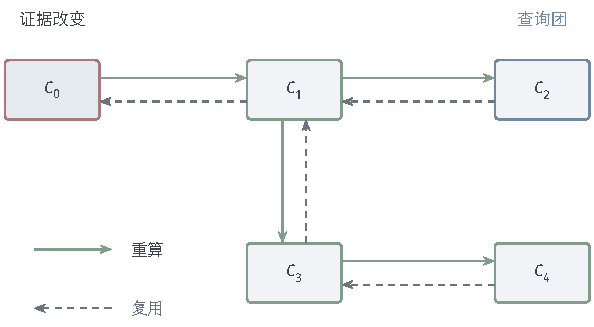
\includegraphics[width=100.651mm]{figures/06-probabilistic-graphical-models/02-inference/tikz/pgm-junction-tree-evidence-update/figure.pdf}
  \caption{单个团势变化后的消息更新。$C_0$改变后，实线方向重新汇总含$C_0$一侧的贡献，反向虚线消息继续复用。查询$C_2$只需更新$C_0-C_1-C_2$路径；其他团表需在其入站消息也更新后才能用于新证据。团的具体变量集合仍须满足运行交集性质。}
  \label{fig:pgm-junction-tree-evidence-update}
\end{figure}

报警例中新观测到$S=0$，变化仅发生在$C_2$。保留$m_{C_1\to C_2}=(0.83,0.17)$，重算$m_{C_2\to C_1}=(0.0095,0.855)$，得到$Z_{\bm e}=p(A=1,S=0)=0.153235$，故障后验为$0.068590/0.153235\approx0.447613$。若将原先单独的报警证据改为$A=0$，反向消息变为$(0.9555,0.0955)$，证据概率为$0.80930$，故障后验为$0.02675/0.80930\approx0.033053$。这两次修改都保留故障侧的先验汇总。

撤回硬证据需要从原始输入恢复团势。旧指示函数已把部分表项置零，对其相除无法找回这些值，因此保留$\phi_C^0$及每条当前证据，按式~\eqref{eq:pgm-junction-tree-local-evidence}重新形成受影响的局部势。随后按源侧依赖重算消息及其缩放常数。若先前还按证据删去变量或裁剪连接，撤回时需一并恢复这些结构。

在原有作用域内修改因子数值，或加入被现有团覆盖的观测似然，都可以沿当前团树更新。新作用域超出现有团时，则要重新分配因子、扩大团或重新三角化，以容纳新增的共同变量。更新后若$Z_{\bm e}=0$，包括硬证据互相矛盾的情形，传播得到零总权重，条件后验没有定义。缓存更新因而同时依赖作用域覆盖、消息来源和正的归一化常数。

\section{算法分析}
\label{sec:pgm-junction-tree-analysis}

\subsection{正确性与校准}
\label{sec:pgm-junction-tree-correctness}

校准给出重叠表的一致性，消息的子树含义则把这些表与原始模型联系起来。下面将一条消息写成源侧全部局部势的求和，进而证明团表确实是所需边缘；同一含义也确定跨团查询的边界和证据更新的依赖范围。

\begin{theorem}[子树消息与团边缘]
  \label{thm:pgm-junction-tree-correctness}
  设$V$为有限变量索引集，每个$X_i$的状态空间有限非空；$\mathcal{T}=(\mathcal{C},\mathcal{E}_{\mathcal T})$是以$V$的子集为团节点、满足$\bigcup_{C\in\mathcal C}C=V$和运行交集性质的有限树。有限个取有限非负值的因子与证据因子恰好各分配给一个覆盖其作用域的团，所得团势为$\phi_C$，并记未归一化目标$q_{\bm e}(\bm{x})=\prod_{C\in\mathcal C}\phi_C(\bm{x}_C)$。对边$(C,D)$，令$S_{C,D}=C\cap D$；删除该边后，记$C$侧的团集合为$\mathcal{C}_{C\mid D}$，并令$U_{C\mid D}=\bigcup_{K\in\mathcal{C}_{C\mid D}}K$。若按式~\eqref{eq:pgm-junction-tree-clique-message}完成全部未缩放和积消息，则对每条有向边$C\to D$，
  \begin{equation}
    m_{C\to D}(\bm{x}_{S_{C,D}})
      =\sum_{\bm{x}_{U_{C\mid D}\setminus S_{C,D}}}
         \prod_{K\in\mathcal{C}_{C\mid D}}\phi_K(\bm{x}_K).
    \label{eq:pgm-junction-tree-subtree-invariant}
  \end{equation}
  完整传播后，定义
  \[
    \begin{aligned}
      B_C(\bm{x}_C)&\mathrel{:=}
        \phi_C(\bm{x}_C)
        \prod_{K\in N_{\mathcal{T}}(C)}
          m_{K\to C}(\bm{x}_{S_{K,C}}),\\
      B_{C,D}(\bm{x}_{S_{C,D}})&\mathrel{:=}
        m_{C\to D}(\bm{x}_{S_{C,D}})
        m_{D\to C}(\bm{x}_{S_{C,D}}),\\
      Z_{\bm e}&\mathrel{:=}
        \sum_{\bm{x}_V}q_{\bm e}(\bm{x}).
    \end{aligned}
  \]
  则对任意团$C$及边$(C,D)$，
  \begin{equation}
    \begin{aligned}
      B_C(\bm{x}_C)
        &=\sum_{\bm{x}_{V\setminus C}}q_{\bm{e}}(\bm{x}),\\
      B_{C,D}(\bm{x}_{S_{C,D}})
        &=\sum_{\bm{x}_{V\setminus S_{C,D}}}q_{\bm{e}}(\bm{x}).
    \end{aligned}
    \label{eq:pgm-junction-tree-true-marginals}
  \end{equation}
  若$Z_{\bm e}>0$，则$B_C/Z_{\bm e}$与$B_{C,D}/Z_{\bm e}$分别为相应的后验团边缘和后验分隔集边缘。
\end{theorem}

\begin{proof}
  按源侧$\mathcal C_{C\mid D}$的团数归纳。若只有叶团$C$，这一侧的全部输入就是$\phi_C$，消去$C\setminus S_{C,D}$即得到式~\eqref{eq:pgm-junction-tree-subtree-invariant}。

  对源侧含多个团的情况，删除$C$后，除$D$侧外的每个邻团$K$各形成一个分支，内部变量为$R_K=U_{K\mid C}\setminus S_{K,C}$。若变量同时出现在该分支和$C$，连接两处的路径经过$K$，运行交集使它属于$S_{K,C}$，所以$R_K$与$C$不交。若两个分支的内部集合共享某变量，连接这两处的路径经过$C$，运行交集又要求它属于$C$，与内部变量定义矛盾。因此各$R_K$彼此也不交。

  要消去的$U_{C\mid D}\setminus S_{C,D}$由$C\setminus S_{C,D}$和各分支内部$R_K$组成。固定$\bm{x}_C$后，这些分支可以分别求和，归纳假设将每一项识别为$m_{K\to C}$。再用有限求和的分配律，可得
  \[
    \begin{aligned}
      &\sum_{\bm{x}_{U_{C\mid D}\setminus S_{C,D}}}
         \prod_{L\in\mathcal{C}_{C\mid D}}\phi_L\\
      &\quad=\sum_{\bm{x}_{C\setminus S_{C,D}}}\phi_C
         \prod_{K\in N_{\mathcal{T}}(C)\setminus\{D\}}
          \left[
            \sum_{\bm{x}_{R_K}}
              \prod_{L\in\mathcal{C}_{K\mid C}}\phi_L
          \right]\\
      &\quad=\sum_{\bm{x}_{C\setminus S_{C,D}}}\phi_C
         \prod_{K\in N_{\mathcal{T}}(C)\setminus\{D\}}m_{K\to C}.
    \end{aligned}
  \]
  该式最后一行就是$C\to D$的更新公式，因此归纳式对整个源侧成立。

  固定任意团$C$，用同样的分解纳入全部邻接分支。它们的内部变量互不重叠，与$C$共同覆盖$V$，局部势又各出现一次，乘积为$q_{\bm e}$。先对各分支内部求和，就留下$\phi_C\prod_Km_{K\to C}=B_C$，得到团边缘等式。再对$C\setminus S_{C,D}$求和，式~\eqref{eq:pgm-junction-tree-local-calibration}给出分隔集边缘$B_{C,D}$。将任一表对其全部状态求和，均得$Z_{\bm e}$；若它为正，归一化即得后验边缘。
\end{proof}

这项证明逐一使用了两个结构条件：运行交集把全部共享变量留在分隔集中，使各分支的内部变量互不重叠；唯一因子分配使局部势的乘积恰为输入模型。于是分配律可以把全局求和拆成消息。仅从一组归一化且相邻一致的表出发，可以重构满足它们的分布，但要确认它就是原模型，还需要上述与原始因子乘积的联系。

在相同的子树分解中，将求和换成最大化，非负因子的分配律给出最大积消息的最优值。给定分隔集状态，回溯表保存的内部选择取得这条消息的值；每次展开时，已有赋值与新分支仅在分隔集中重叠。沿树代入这些选择，最终配置的联合权重就达到根的最大值。根最大值为零时，全部配置的权重都为零，条件分布及其条件MPE均没有定义。

因子和消息可以含零表项，和积与最大积证明都仍成立；正表项主要便于采用比值形式重构。连续变量的和积消息改用积分，需要合适的密度、有限且为正的归一化常数，以及能够精确计算的局部积分。Tonelli定理允许交换非负函数的积分次序，实际积分表达仍取决于函数形式。连续观测还需要相应的条件密度或观测模型，单点指示函数在通常连续测度下无法直接产生离散硬证据那样的概率质量。

\subsection{与变量消除的关系}
\label{sec:pgm-junction-tree-ve-relation}

三角化记录了变量消除产生的共同作用域。消去$v_i$时，相关因子的乘积作用域包含在$\{v_i\}\cup N_i^+$中，输出以剩余邻居$N_i^+$为边界。保存每个消元集合及其生成的新因子，就可以记录这些局部计算之间的消息依赖。最大权团树选择进一步为极大团之间确定满足运行交集的连接（参见\BookTheoremRef{thm:graph-theory-clique-tree-maximum-weight}{卷1《数学准备：计算、分析与几何》第9章“图的表示与计算”第9.3.2.3节“弦图条件下的无填充分解”}）。

收缩被相邻较大集合包含的非极大集合，相当于将数步局部消元合并为一次团间计算，得到更紧凑的团树。此时一条极大团间消息可以汇总连续消去的多个变量，消息与单个消元步骤之间未必一一对应。

从团树也可以恢复消元过程。选定根后，在叶团中消去不属于父分隔集的变量；运行交集保证这些变量已不在其他未处理团中出现。把生成的分隔集因子送入父团，继续处理，便完成收集阶段。因此两种算法使用同样的乘法和边缘化，并由同样的子问题分解保证精确性。

以报警例的$C_1=\{F,H\}$为根时，先在$C_2$内用报警指示函数固定$A$，再对$A,S$求和形成$u(h)$；根结合自身势，再消去$H$得到故障查询。以$C_2$为根时，$C_1$消去$F$形成$v(h)$。保存这两个方向的表，后续就能读取$F,H,S$的边缘，避免重新进行故障侧或报警侧的消元。

查询次数决定了保存消息的收益。只求一次目标边缘时，变量消除可以及时释放已经用完的中间表，收集到目标位置即可。固定模型上反复读取不同位置的边缘，或多次局部修改证据时，团树的双向消息提供持续复用。缓存同样可以用于变量消除；团树将它组织成明确的源侧依赖和失效规则\scite{pgm-koller2009}

\subsection{复杂度与适用边界}
\label{sec:pgm-junction-tree-complexity}

一轮传播只发送与树边数成正比的消息，每张消息的计算量还取决于团的状态空间。令$k=|\mathcal C|$、$r_i=|\mathcal X_i|$，团表和分隔集表分别有
\begin{equation}
  r_C=\prod_{i\in C}r_i,\qquad
  r_{C,D}=\prod_{i\in S_{C,D}}r_i.
  \label{eq:pgm-junction-tree-table-sizes}
\end{equation}
发送$C\to D$输出$r_{C,D}$个数。通用稠密实现通常先遍历$r_C$个团状态，组合势和各入站消息，再累加到对应的分隔集状态。因此，即使分隔集表很小，形成它仍可能需要枚举一个大团。

若团$C$的度为$\deg(C)$，逐条出站消息都重乘其余入站消息，会重复执行$O(\deg(C)^2r_C)$次乘法。可以对每个团状态计算入站值的前缀积和后缀积，以$O(\deg(C))$次乘法得到排除任意邻居的乘积，再分别累加。这种做法保留零表项，避免除以某个零消息。配合收集和分发，完整传播的时间上界为
\begin{equation}
  O\!\left(\sum_{C\in\mathcal{C}}(\deg(C)+1)r_C\right),
  \label{eq:pgm-junction-tree-time}
\end{equation}
这个上界从已建好的局部势开始计算，并假定表索引等基本操作成本有界；$+1$计入形成团汇总表的遍历。如果每条消息各自重新组合全部输入，则还需计入重复乘法产生的度数因子。

局部势、团汇总表以及边的两个方向消息需要持久保存，内存规模为
\begin{equation}
  O\!\left(
    \sum_{C\in\mathcal{C}}r_C+
    2\sum_{(C,D)\in\mathcal{E}_{\mathcal{T}}}r_{C,D}
  \right),
  \label{eq:pgm-junction-tree-memory}
\end{equation}
输入因子、工作空间和最大积回溯表需另外计入。前缀积与后缀积可逐个团状态临时计算，使用后释放。只保存消息、查询时再重建团表，也可减少持久存储的常数开销；每张实际需要的稠密团表仍取决于团状态数。

若单变量状态数至多为$r$，所选三角化的最大团大小为$w+1$，则$r_C\le r^{w+1}$。树上$\sum_C\deg(C)=2(k-1)$，代入式~\eqref{eq:pgm-junction-tree-time}得到$O(kr^{w+1})$；对$m$个原始因子，按稠密表建立局部势的保守成本为$O(mr^{w+1})$。不同极大团的分隔集至多含$w$个变量，因此消息表至多有$r^w$项，团势表则至多有$r^{w+1}$项。这里$w$属于已选顺序，最优三角化才使它等于原交互图的树宽。

变量状态数不同时，同样大小的团也可能需要不同规模的表。对图~\ref{fig:pgm-junction-tree-triangulation}中的四环，取$r_1=r_3=10$、$r_2=r_4=2$，表~\ref{tab:pgm-junction-tree-triangulation-cost}展示两种填充选择。两个方案都产生三变量团，但团表和分隔集表项数显著不同，因此排序时还需考虑各变量状态数。

\begin{table}[htbp]
  \centering
  \begin{tabular}{cccc}
    \toprule
    填充边 & 极大团 & 各团表项数 & 分隔集表项数\\
    \midrule
    $1-3$ & $\{1,2,3\},\{1,3,4\}$ & $200,\;200$ & $100$\\
    $2-4$ & $\{1,2,4\},\{2,3,4\}$ & $40,\;40$ & $4$\\
    \bottomrule
  \end{tabular}
  \caption{四环的两种三角化及其表规模。人工设置$r_1=r_3=10$、$r_2=r_4=2$，两种方案的未加权树宽同为$2$，但填充边$2-4$对应的团表与消息表更小。}
  \label{tab:pgm-junction-tree-triangulation-cost}
\end{table}

大团很快会占满内存：$30$个二元变量组成的团有$2^{30}$个表项，一张双精度表就占$8$\,GiB，还需保存其他团、消息和工作空间。最大权选树发生在极大团形成之后，无法缩小这些表。单团证据变化最坏仍需向全树传播；跨团联合查询还要进行子树内消元，并写出可能很大的查询表。

上述指数界针对稠密离散表表示。满足积分条件的高斯势使用精度矩阵和一次项，消息通过块矩阵消元形成，成本取决于矩阵维数和填充。紧凑表示依赖函数族在乘法与积分下保持闭包；混合分量增加或一般非线性势可能使消息变得更复杂。因此评估成本时，应把实际的局部积分、最大化或枚举方式一并计入。

团树适用于作用域固定、可摊销编译成本且团表可容纳的重复推断。稠密团表的规模过大时，需要改用更紧凑的函数表示或近似推断。第~\ref{sec:pgm-variational-bethe}节会讨论直接在含环图上迭代消息的方法；那时分支可能重叠，须另行分析固定点和近似误差。

\section{本章小结}
\label{sec:pgm-junction-tree-summary}

消息将一侧子问题的内部变量汇总掉，保留后续计算所需的边界状态。因子树可以直接按边切分，一般图则先以道德化和三角化确定共同作用域，再将团连成运行交集树。共享变量沿路径连续保留，原始因子各分配一次，这两项条件使消息能够精确组合为原模型的边缘。

收集汇总根的各侧贡献，分发为其他团补齐根侧信息。若$Z_{\bm e}>0$，$B_C/Z_{\bm e}$给出团的后验边缘，$\phi_C$继续保存本团的原始输入。单团覆盖的查询在团内求和；跨团查询借助边界消息继续消元，或用分隔集势修正重叠权重。MPE另用最大积消息和回溯表恢复最优配置。证据改变时，按源侧依赖更新缓存；撤回硬证据则从原始团势恢复输入。

团树保存的不仅是数值结果，还有每张表与局部因子的依赖关系，使多次查询和局部更新可以共享已经完成的计算。最大团的状态空间、各变量状态数和查询输出大小仍决定存储与算术成本，缓存主要节省重复消元的工作。

\paragraph{扩展阅读}
Lauritzen与Spiegelhalter的局部计算论文介绍如何通过图变换组织概率计算，Koller与Friedman的教材系统推导团树传播。两者可结合本章的子树不变量阅读：运行交集确定完整边界，证据分配确定输入乘积，校准则给出共享变量上一致的边缘\scite{pgm-overview-lauritzen1988,pgm-koller2009}

\chapter{变分推断与确定性近似}
\label{chap:pgm-variational}

第~\ref{chap:pgm-elimination}章的变量消元和第~\ref{chap:pgm-junction-tree}章的团树传播，都是\emph{精确}推断：它们在数学上给出后验边缘和配分函数的准确值。但前面已经反复看到一个瓶颈——计算成本取决于消元过程中出现的最大因子（诱导宽度）。一旦图比较稠密，这个中间团可能包含很多变量，精确推断的时间和存储随团的大小\emph{指数}增长，在现实规模的模型上根本算不动。既然精确答案要不起，一个自然的妥协是\emph{主动放弃一部分精确性、换取可承受的计算量}，但要用可量化的方式做这件事，并能说清近似误差来自哪里。

本章的近似方法沿两条性质不同的路线展开，对应两类不同的查询。第一条针对\textbf{分布查询}（“故障的后验概率是多少”“某统计量的后验期望是多少”）：我们仍然要保留完整的概率与不确定性，做法是\emph{限制后验分布的表达形式}——不在所有可能分布里找后验，而是在一个简单、好算的分布族（如独立乘积分布、高斯）里挑一个“最接近”真实后验的，这就是变分推断。第二条针对\textbf{配置查询}（“所有变量最可能取哪一组值”，即MPE）：此时只要一个最优配置、不需要完整分布，做法是\emph{放宽离散配置的约束}，先把它变成一个更容易解的连续优化问题，再从松弛解恢复出合法配置。两条路线输出不同、误差也要分别衡量。

消元和团树通过中间因子保存变量之间的依赖（第~\ref{chap:pgm-elimination}、\ref{chap:pgm-junction-tree}章）。局部因子虽然很小，中间团却可能包含许多变量，使联合推断的时间和存储成本迅速增长。面对这一瓶颈，我们可以限制后验分布的表达形式，在可计算的分布族中寻找近似；若任务只需要一组最可能的配置，则可以放宽配置约束，先求解较容易的连续优化问题。前一条路线保留概率和不确定性，后一条路线选择离散配置，其误差需要分别衡量。

本章设模型参数已知。对于观测$\bm{x}$和潜变量$\bm{z}$，分布查询以$p(\bm{z}\mid\bm{x})$为目标，计算边缘概率和期望；近似方法可能输出全局分布、局部概率表或高斯近似。配置查询则将证据吸收到因子中，为全部未观测变量选择一组联合最优值，即最可能解释（most probable explanation, MPE）。围绕这两类查询，后文依次讨论近似对象的选择、优化求解与误差诊断。

\section{变分推断的统一视角}

\label{sec:pgm-variational-unified}
\label{sec:pgm-variational-duality}

设备报警后，要判断故障有多大可能，我们需要的是给定报警的状态分布，而不是先选定一种故障状态。推广到一般模型，固定观测$\bm x$和模型参数，用随机向量$\bm Z$表示尚未观测、需要推断的变量。联合模型给出了各个配置的权重$p(\bm x,\bm z)$，后验则要把这些权重归一化：
\[
  \pi(\bm z):=p(\bm z\mid\bm x)
    =\frac{p(\bm x,\bm z)}{p(\bm x)},
  \qquad p(\bm x)=\int p(\bm x,\bm z)\,d\bm z.
\]
本章用积分统一表示连续与离散情形；离散变量的积分改为求和。假设$0<p(\bm x)<\infty$；连续观测下，$p(\bm x)$是观测位置的边缘密度。单个配置的联合权重即使容易评价，累加所有配置仍可能很昂贵。例如，$d$个二元未知变量共有$2^d$种配置；局部分解可减少重复运算，但消元中出现的大团仍可能使计算难以承受。连续变量还可能留下无法解析计算的高维积分。

既然精确后验求不出来，变分法的核心思路是“\emph{用一个好算的分布去近似它}”。但这里立刻冒出两个必须回答的问题：一是用什么标准衡量“近似得像不像”，二是这个标准里仍含着我们算不出的$p(\bm x)$，怎么把它消掉。下面先建立近似分布与候选族的概念，再一步步推出可实际优化的ELBO。如果暂时无法求出$\pi$，可以先构造一个容易查询的分布$q$，用它给同一组未知变量分配概率。对设备模型，固定$A=1$后，$q$仍是$(F,H,S)$上的联合分布，故障概率就用$q(F=1)$近似。若查询的是某个实值统计量$f(\bm Z)$的后验期望，则用$\mathbb E_q f(\bm Z)$近似$\mathbb E_\pi f(\bm Z)$，两者均须存在。这里改变的是计算所用的分布，观测和原模型保持固定。只输出一个配置无法保留这些概率与期望，因此$q$需要描述未知变量的整个分布。

接下来要决定允许使用哪些$q$，以及怎样选出其中较合适的一个。记候选分布族为$\mathcal Q$；例如可用高斯的均值和协方差调整$q$，也可用每个二元变量取$1$的概率规定一个独立乘积分布。若候选写成$q_{\bm\lambda}$，$\bm\lambda\in\Lambda$就是待调整的分布参数，$\Lambda$包含方差为正或概率位于$[0,1]$等约束。调整$\bm\lambda$便是在候选族中选择一个分布，这就是\term{变分推断}（variational inference, VI）将后验计算改写为分布优化的含义\scite{bishop2006,pgm-cmu2017-vi}。

选择$q$需要一个比较准则。反向KL以$q$为积分权重，衡量它与目标后验$\pi$的差异；两者相同时KL为零。因此，我们希望在$\mathcal Q$中减小$D_{\mathrm{KL}}(q\Vert\pi)$。“反向”指参数顺序；本章的$D_{\mathrm{KL}}$和$\operatorname{KL}$表示同一散度。若改用$D_{\mathrm{KL}}(\pi\Vert q)$，期望要在难以查询的真实后验下计算。反向KL把期望放到我们能够控制的$q$下，但它的定义仍含未知的$p(\bm x)$，还需要消去这个计算障碍。

将$\pi(\bm z)=p(\bm x,\bm z)/p(\bm x)$代入KL。因为$\bm x$固定，$\log p(\bm x)$对所有$\bm z$都是同一个常数，又因为$q$的总质量为$1$，便有
\[
  \begin{aligned}
    D_{\mathrm{KL}}(q\Vert\pi)
      &=\mathbb E_q\log\frac{q(\bm Z)}{p(\bm x,\bm Z)}
          +\log p(\bm x)\\
      &=\log p(\bm x)
          -\mathbb E_q\log\frac{p(\bm x,\bm Z)}{q(\bm Z)}.
  \end{aligned}
\]
这一步把目标拆成两项：第一项对所有候选$q$相同，第二项只涉及联合权重和候选分布。比较候选时无需知道第一项的数值，只要增大第二项，就会减小KL。于是将第二项记为证据下界（evidence lower bound, ELBO）：
\begin{equation}
  \begin{aligned}
    \mathcal L(q)
      &:=\mathbb E_q\log\frac{p(\bm x,\bm Z)}{q(\bm Z)},\\
    \log p(\bm{x})
      &=\mathcal L(q)+D_{\mathrm{KL}}(q\Vert\pi).
  \end{aligned}
  \label{eq:pgm-variational-elbo}
\end{equation}
KL非负，所以$\mathcal L(q)\leq\log p(\bm x)$；这解释了“下界”的名称。最大化ELBO同时选择了反向KL意义下更接近后验的候选，而不仅是在估计证据。若采用参数化候选，实际求解的是$\max_{\bm\lambda\in\Lambda}\mathcal L(q_{\bm\lambda})$；所学的是近似后验的参数，原模型参数仍然固定。分布逼近准则、指数族矩表示与最大熵对偶的背景可参考\BookChapterRef{chap:information-theory-and-statistical-geometry}{卷2《数学准备：概率、因果与决策》的“概率分布的分析与优化”章}。下面在本章推断问题中说明所需的关系。

上述有限值分解要求$q\ll\pi$且$D_{\mathrm{KL}}(q\Vert\pi)<\infty$，即$q$不在后验概率为零的集合上放置正质量，并满足相应可积性。这里将ELBO定义为整体对数比的期望；只有两项分别有定义时，才进一步拆成$\mathbb E_q\log p(\bm x,\bm Z)+H(q)$。KL无限时可令ELBO取$-\infty$，但不能在原分解中相加无穷项。消去$p(\bm x)$也不自动保证ELBO容易计算：还需让$q$下的这些期望可以解析求出，或能用采样估计。近似族与计算方法正是围绕这一要求共同选择的\scite{pgm-stanford-cs228-variational}。

从近似族到实际解，还要经过目标选择和数值优化。若$\mathcal Q$无法表示后验，其最优解$q^\star$也会留下近似误差；换用正向KL或矩匹配，则改变了衡量分布差距的准则。对于选定的ELBO，算法得到$\widehat q$后，$\mathcal L(q^\star)-\mathcal L(\widehat q)$衡量尚未消除的优化误差；最优值未取得时，以上确界代替$\mathcal L(q^\star)$。增加迭代主要作用于这一优化差距，近似族的表达限制仍由$\mathcal Q$决定。

反向KL只在$q$分配质量的位置计算对数密度比。若$q$在目标概率为零的区域放置正质量，KL为无穷大；获得有限值要求$q$避开这些区域。这种支持限制称为\term{零强制}（zero forcing），即目标为零迫使近似也为零。正向$\operatorname{KL}(p\Vert q)$的积分权重来自$p$，获得有限值要求$q$覆盖目标的正质量区域，称为\term{零回避}（zero avoiding）。两个名称均描述$q$受到的支持限制\scite{bishop2006}。

支持限制也为模态选择提供了直觉。若正密度目标的两个模态之间存在深谷，单峰$q$同时覆盖两者时，可能在谷底放置较多质量，从而增大反向KL。集中于一个模态可减少这部分代价，因此某些受限近似族会遗漏其他模态。这一倾向取决于目标形状和近似族；足够丰富的混合分布仍可表示多个模态。

相关高斯给出了近似族限制影响方差的可解析例子。设目标$p$是零均值二维高斯，协方差为
\[
  \bm{\Sigma}=
  \begin{pmatrix}1&r\\r&1\end{pmatrix},
  \qquad |r|<1,
\]
并限制$q=\mathcal N(\bm{m},\operatorname{diag}(v_1,v_2))$，其中$v_1,v_2>0$。这个限制允许调整两个边缘的均值和方差，却不能用协方差表达目标中的相关性。记精度矩阵为
\[
  \bm\Lambda=\bm\Sigma^{-1}
    =\frac{1}{1-r^2}
      \begin{pmatrix}1&-r\\-r&1\end{pmatrix}.
\]
将两个高斯的对数密度代入反向KL，并使用$\mathbb E_q\bm Z=\bm m$及$\operatorname{Cov}_q(\bm Z)=\operatorname{diag}(v_1,v_2)$，得到
\[
  \operatorname{KL}(q\Vert p)
    =\frac12\left\{
       \bm m^\top\bm\Lambda\bm m
       +\sum_i\bm\Lambda_{i,i}v_i-2
       +\log\det\bm\Sigma-\sum_i\log v_i\right\}.
\]
其中$-2+\log\det\bm\Sigma$只依赖固定目标。舍去这类与候选参数无关的常数后，需要最小化的有关项为
\[
  \frac12\left\{\bm{m}^{\top}\bm{\Lambda}\bm{m}
     +\sum_i\bm{\Lambda}_{i,i}v_i-\sum_i\log v_i\right\}.
\]
均值项的梯度为$\bm\Lambda\bm m$；$\bm\Lambda$正定，因此这一项在$\bm m=\bm0$处取得唯一最小值。每个方差项的导数为$\tfrac12(\bm\Lambda_{i,i}-1/v_i)$，二阶导数为$1/(2v_i^2)>0$。令一阶导数为零，便得到唯一最优方差
\[
  v_i=\frac{1}{\bm\Lambda_{i,i}}=1-r^2.
\]

取$r=0.8$时，目标的两个边缘方差均为$1$，最优独立近似却均为$0.36$。二维高斯中，给定另一坐标后的条件方差为$1-r\cdot1^{-1}\cdot r=1-r^2$，恰好等于这里的独立近似方差。它比目标的边缘方差更小。

换成正向$\operatorname{KL}(p\Vert q)$时，积分权重来自目标$p$。因为目标每个坐标的均值为$0$、二阶矩为$1$，依赖候选参数的部分变成
\[
  \frac12\sum_i\left\{\log v_i+\frac{1+m_i^2}{v_i}\right\}.
\]
对固定$v_i$，$m_i^2/v_i$在$m_i=0$处最小；代回后，对$v_i$求导得到$\tfrac12(1/v_i-1/v_i^2)$，其符号在$v_i=1$两侧由负变正。于是正向KL的最优解匹配边缘矩，得到$\bm m=\bm0$和$v_i=1$。因此，在这一相关高斯和独立高斯近似族的设定下，反向KL最优解低估边缘方差；结论的范围由这两个分布族共同限定。

优化整个$q$后，可以由它计算各个节点或因子的边缘概率。不过，许多查询只需这些小表，我们也希望直接以局部概率表作为优化变量。两种表示怎样连接？对离散节点，事件$Z_i=k$的概率等于指示函数$\mathbb I\{Z_i=k\}$的期望；一组变量的联合配置概率同样可以这样表示。将所需指示函数收集为统计量向量$\bm T$，其期望就收集了局部概率表。下面先用指数族说明模型得分怎样作用于这些期望，再检查哪些局部表能够来自同一个联合分布。记自然参数为$\bm\theta$，它在此表示固定模型的得分系数：
\begin{equation}
  \begin{aligned}
    p_{\bm{\theta}}(\bm{z})
      &=h(\bm{z})\exp\{\langle\bm{\theta},\bm{T}(\bm{z})\rangle
                      -A(\bm{\theta})\},\\
    A(\bm{\theta})
      &=\log\int h(\bm{z})
          e^{\langle\bm{\theta},\bm{T}(\bm{z})\rangle}\,d\bm{z}.
  \end{aligned}
  \label{eq:pgm-variational-exponential-family}
\end{equation}
$h$为不依赖参数的基准项，$A$为对数配分函数。

要由模型参数读出这些局部概率，需要计算$\bm T$的期望。自然参数位于$A<\infty$的开域内且可交换微分与积分时，对归一化积分求导，再除以该积分，得到
\[
  \frac{\partial A}{\partial\theta_j}
    =\frac{\int T_j(\bm z)h(\bm z)
                  e^{\langle\bm\theta,\bm T(\bm z)\rangle}\,d\bm z}
           {\int h(\bm z)e^{\langle\bm\theta,\bm T(\bm z)\rangle}\,d\bm z}
    =\mathbb E_{\bm\theta}T_j(\bm Z).
\]
再次对$\theta_k$求导时，分子的导数产生$\mathbb E(T_jT_k)$，分母的导数产生$\mathbb E T_j\mathbb E T_k$。两项相减就是协方差，因此
\begin{equation}
  \nabla A(\bm{\theta})=\mathbb E_{\bm{\theta}}\bm{T}(\bm{Z})
      =:\bm{\mu},\qquad
  \nabla^2 A(\bm{\theta})
      =\operatorname{Cov}_{\bm{\theta}}[\bm{T}(\bm{Z})].
  \label{eq:pgm-variational-moments}
\end{equation}
$\bm{\mu}$称为\term{均值参数}（mean parameter），直接记录期望统计量。

均值参数能否反过来确定自然参数，取决于统计量是否重复记录了同一信息。例如，若保留某节点全部状态的指示函数，就恒有$\sum_k\mathbb I\{Z_i=k\}=1$。沿这些自然参数同时加上同一个常数，只会把每个配置的未归一化权重乘以同一常数；归一化后的分布和均值参数都不改变。这就是一条仿射冗余：某个非零系数向量$\bm a$使$\langle\bm a,\bm T(\bm z)\rangle$在共同支持上几乎处处为常数。

式~\eqref{eq:pgm-variational-moments}还说明了冗余为何产生Hessian零方向，因为
\[
  \bm a^\top\nabla^2A(\bm\theta)\bm a
    =\operatorname{Var}_{\bm\theta}
          [\langle\bm a,\bm T(\bm Z)\rangle]=0.
\]
删去这些关系中可由其余统计量和常数表示的冗余分量，保留足以表示同一分布族的一组统计量，便得到这里所需的最小表示。在共同支持上密度为正、协方差存在且上述求导有效时，最小表示中的每个非零方向都有正方差，Hessian因而正定。自然参数取合法开域中的有限值时，逆函数定理便给出$\bm\theta\mapsto\bm\mu$的局部一一对应。

这里的内部条件同时限定参数和待匹配的矩。我们要求使用合法开域中的有限自然参数，并要求目标矩属于这些参数能够实现的内部均值域；仅仅写下一组数值，并不能保证它们是该分布族的矩。下文的有限离散模型在删除仿射冗余后，其内部均值域就是可实现集合的相对内部，即在该集合实际所在的仿射空间内取内部。边界矩可能仍能由某个分布实现，却只能由指数族中的参数极限逼近，不能套用上述局部可逆性。

将局部表直接当作优化变量时，逐表归一化还不够。例如，两个表若都包含同一节点，却给该节点不同的边缘概率，就不可能来自同一个联合分布。我们因此需要描述所有可由联合分布实现的统计量期望。以下对偶与多面体陈述先限定为有限离散状态、$h=1$。以$V=\{1,\ldots,d\}$记节点集，$Z_i$的有限非空状态集为$\mathcal X_i$，节点集$A\subseteq V$上的配置集为$\mathcal X_A=\prod_{i\in A}\mathcal X_i$，全部联合配置组成$D=\mathcal X_V$。定义\term{边缘多面体}（marginal polytope）
\begin{equation}
  \mathcal M
    =\left\{\mathbb E_q\bm{T}(\bm{Z}):q\text{为全局分布}\right\}
    =\operatorname{conv}\{\bm{T}(\bm{z}):\bm{z}\in D\},
  \label{eq:pgm-variational-marginal-polytope}
\end{equation}
其中$\operatorname{conv}$表示凸包。这个等号来自$\mathbb E_q\bm T=\sum_{\bm z\in D}q(\bm z)\bm T(\bm z)$：概率$q(\bm z)$是非负且总和为$1$的凸组合系数；反过来，每一组这样的系数都定义一个全局分布。当$\bm{T}$由节点和因子配置的指示函数组成时，$\bm{\mu}$就是相应边缘概率。$\mathcal M$要求这些局部表格能够同时来自某个全局分布，而不只是每张表各自归一化。

有了可实现的均值参数，还要说明为什么只看期望得分不足以计算配分函数。在当前有限离散、$h=1$的设定下，对任意全局分布$q$，将$p_{\bm\theta}$代入KL可得
\[
  \operatorname{KL}(q\Vert p_{\bm\theta})
    =A(\bm\theta)-\langle\bm\theta,\mathbb E_q\bm T\rangle-H(q).
\]
KL非负，且$q=p_{\bm\theta}$时取零，所以在所有$q$中最大化期望得分加熵，恰好得到$A(\bm\theta)$。这里的熵保留了不同配置共同贡献的概率质量；只取一个配置的得分，还没有累计这些贡献。

现在按$\mathbb E_q\bm T=\bm\mu$将候选分布分组。同一组中，$\langle\bm\theta,\bm\mu\rangle$完全相同，差别只在熵，因此先选这一组中熵最大的分布，再比较不同的$\bm\mu$。对$\bm\mu\in\mathcal M$，令$H^\star(\bm\mu)=\max_{q:\mathbb E_q\bm T=\bm\mu}H(q)$，即满足这些统计量约束的分布所能达到的最大熵。有限状态下，约束分布集合非空且紧，熵连续，所以这一最大值存在。这样便得到
\begin{equation}
  A(\bm\theta)=\max_{\bm\mu\in\mathcal M}
    \{\langle\bm\theta,\bm\mu\rangle+H^\star(\bm\mu)\}.
  \label{eq:pgm-variational-gibbs}
\end{equation}
这一优化包含$\mathcal M$的边界，不要求每个候选均值都由有限自然参数实现。例如，对单个伯努利变量取$T(z)=z$，确定性分布$q(Z=1)=1$给出边界均值$\mu=1$和熵$0$；有限自然参数产生的概率$e^\theta/(1+e^\theta)$始终小于$1$，只有$\theta\to+\infty$才到达该边界极限。边界仍是合法候选，因为这里的优化域由所有全局分布确定。

还可以反过来，固定$\bm\mu$，考察线性项减去对数配分函数所得的差值，并在自然参数上取上确界：
\[
  A^*(\bm\mu)
    :=\sup_{\bm\theta}
          \{\langle\bm\theta,\bm\mu\rangle-A(\bm\theta)\}.
\]
这个函数称为$A$的凸共轭。式~\eqref{eq:pgm-variational-gibbs}说明，对可实现的$\bm\mu$，花括号中的量始终不超过$-H^\star(\bm\mu)$。有限离散模型的熵对偶进一步给出
\[
  A^*(\bm\mu)=
    \begin{cases}
      -H^\star(\bm\mu),&\bm\mu\in\mathcal M,\\
      +\infty,&\bm\mu\notin\mathcal M.
    \end{cases}
\]
内部均值处，可以用实现最大熵分布的自然参数达到等号；边界处需要允许上确界由参数极限实现。这一关系的用途是把分布优化改写为均值坐标上的优化：可实现性由$\mathcal M$承担，分布在相同矩约束下还能保留多少不确定性由$H^\star$承担。该表示因此将图推断的困难集中到可行域$\mathcal M$和最大熵$H^\star$上。

凸共轭中的负熵对应给定统计量约束下的最大熵。少量边缘统计量通常容许多个全局分布；这些分布具有相同的得分期望，熵却可能不同，故它们各自的熵未必等于$H^\star$。基准项为一般$h$时，熵项相应变为$H(q)+\mathbb E_q\log h$。连续变量还涉及可积性、闭性和对偶成立条件，其均值可实现集合通常也超出有限多面体的范围。指数族与变分对偶的系统论述见Wainwright和Jordan\scite{pgm-wainwright2008}。

式~\eqref{eq:pgm-variational-gibbs}中的计算困难有两个来源：描述$\mathcal M$可能需要大量全局一致性约束，计算$H^\star$可能需要恢复联合分布。平均场限制全局分布族并计算真实熵，从而得到对数配分函数下界；局部自由能方法则同时近似可行集合和熵，界的方向取决于具体构造。对于配置优化，目标中没有熵，扩大可行集合直接给出最大得分上界。

同一坐标也能表示MPE。令$S(\bm z)=\langle\bm{\theta},\bm T(\bm z)\rangle$为吸收证据后的有限离散得分，$D$为全部未观测变量的完整配置集合，则
\begin{equation}
  \max_{\bm z\in D}S(\bm z)
    =\max_{\bm{\mu}\in\mathcal M}
       \langle\bm{\theta},\bm{\mu}\rangle.
  \label{eq:pgm-variational-mpe}
\end{equation}
这一等号可直接由凸组合看出：任意$\bm\mu\in\mathcal M$都给出$\langle\bm\theta,\bm\mu\rangle=\sum_{\bm z}q(\bm z)S(\bm z)$，加权平均不超过最大配置得分；把$q$集中在某个最大得分配置上，又能取到这个最大值。右侧没有熵项，因为答案只需保留一个最大得分配置，而无须累计其他配置的概率质量。对数配分函数查询若替换$\mathcal M$或$H^\star$，误差落在分布、边缘或归一化常数上；MPE若扩大$\mathcal M$，则得到连续松弛及最大得分上界，还必须从松弛解恢复合法配置。这正是两条主线共享几何表示而输出、保证和诊断不同的原因。

共同的统计量坐标便于比较近似方法所改变的对象。拉普拉斯近似用众数附近的二阶展开替代对数密度，EP通过临时放回真实因子后的分布匹配矩，两者将在第~\ref{sec:pgm-variational-laplace-ep}节说明。LP从无熵的式~\eqref{eq:pgm-variational-mpe}出发，放宽配置的一致性约束（第~\ref{sec:pgm-variational-lp}节）。这三种机制分别改变密度形状、局部矩和可行集合，对应不同的误差与诊断。

\begin{example}[三角图的精确基准]
  \label{ex:pgm-variational-triangle}
  以下人工构造的二元模型贯穿本章。三个变量$Z_i\in\{0,1\}$组成三角图，每条边奖励端点取不同值：
  \begin{equation}
    p_\beta(\bm{z})=\frac{\exp S_\beta(\bm{z})}{Z_\beta},
    \qquad
    S_\beta(\bm{z})
      =\beta\sum_{(i,j)\in E}\mathbb I[z_i\ne z_j],
    \quad \beta=\log2.
    \label{eq:pgm-variational-triangle}
  \end{equation}
  两个全相同配置的得分为$0$，其余六个配置恰有两条不相等边，得分为$2\beta$。将八个配置的权重相加，得到
  \[
    Z_\beta=2+6e^{2\beta}=26.
  \]
  接着固定边$(1,2)$的状态，只对$Z_3$求和。若$(Z_1,Z_2)=(0,0)$，$Z_3=0$和$Z_3=1$的权重分别为$1$和$e^{2\beta}=4$，所以这一边状态的边缘概率为$5/26$。若$(Z_1,Z_2)=(0,1)$，无论$Z_3$取何值，都恰有两条异值边；两个权重均为$4$，相加得到$8/26=4/13$。同时翻转全部变量不会改变得分，因此$(1,1)$与$(0,0)$同概率，$(1,0)$与$(0,1)$同概率。每条边的概率表于是为
  \[
    p_\beta(Z_i,Z_j)=
      \begin{pmatrix}5/26&4/13\\4/13&5/26\end{pmatrix},
      \qquad (i,j)\in E,
  \]
  其中行、列依次按状态$0,1$排列。由表格沿任一行或列求和，得到$p_\beta(Z_i=1)=5/26+4/13=1/2$；将两个非对角项相加，得到$p_\beta(Z_i\ne Z_j)=8/13$。每条边的两个同值状态$(0,0)$与$(1,1)$因而各有概率$5/26$，两个异值状态$(0,1)$与$(1,0)$各有概率$4/13$。节点边缘都是均匀的，但节点并不独立；三个二元变量也不可能在每条边上都取不同值：若$Z_1\ne Z_2$且$Z_2\ne Z_3$，二元性就迫使$Z_1=Z_3$，与第三条边也要求异值矛盾。
\end{example}

图~\ref{fig:pgm-variational-triangle}把同一模型的三种描述并列起来。中间面板使用本例的均匀平均场解，即每个$q_i(Z_i=1)=1/2$；后文将求出这个解并检查它的最优性。在这个特定乘积分布中，一条边取不同值的概率是$1/2$。一般乘积分布的这一概率还会随两个节点的边缘改变，不能仅由完全因子化就断定为$1/2$。完全因子化近似丢失节点相关性，局部一致表则可能提出无法共同实现的边缘。后文用这个模型分别检查分布近似和配置松弛的误差。
\begin{figure}[htbp]
  \centering
  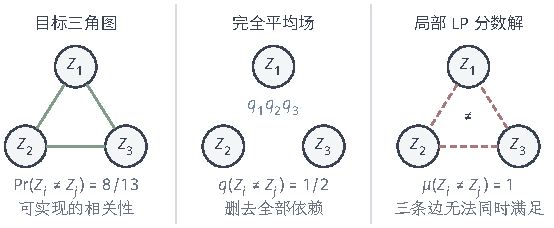
\includegraphics[width=92.445mm]{figures/06-probabilistic-graphical-models/02-inference/tikz/pgm-variational-triangle/figure.pdf}
  \caption{三角图、完全因子化分布和局部一致的边缘表。中间为本例均匀平均场解$q_i(Z_i=1)=1/2$，其边异值概率为$1/2$。右侧让每条边都以概率$1$取不同值，节点边缘仍都是$(1/2,1/2)$；它满足局部一致性，却不可能由任何全局二元分布实现。}
  \label{fig:pgm-variational-triangle}
\end{figure}

\section{近似后验分布与边缘概率}

\label{sec:pgm-variational-posterior}

后验分布或边缘概率难以精确求出时，需要回答三个问题：怎样构造可计算的近似，怎样求出这个近似，以及它能否可靠地回答所需的查询。下面依次讨论后验分布与边缘概率的近似、近似的计算和近似的可靠性。

\subsection{后验分布与边缘概率的近似}
\label{sec:pgm-variational-laplace-ep}

限制全局分布、放宽局部边缘的一致性、匹配分布矩和近似局部曲率，改变的是不同的概率对象与近似准则。各方法的更新公式在构造中一并给出；随后再讨论如何组织这些计算。

\subsubsection{基于因子化分布的近似}

\label{sec:pgm-variational-mean-field}
\label{sec:pgm-variational-mean-field-structured}
\label{sec:pgm-variational-coordinate}

完整联合概率表要记录每一种变量组合，$d$个二元变量就需要$2^d-1$个自由概率，这正是精确推断扛不住的原因。最简单的“砍参数”办法是假设推断时各变量\emph{相互独立}：只保存每个变量自己的边缘分布（$d$个二元变量只需$d$个数），再把它们相乘当作联合分布。这样做当然丢掉了变量之间的相关性——但原模型里的耦合并没有消失，它会在逐个更新某个变量时、通过“其他变量的期望”重新进入计算。\term{平均场近似}（mean-field approximation）采用
\[
  q(\bm{z})=\prod_{i=1}^{d}q_i(z_i).
\]
在$q$中，各变量相互独立，条件分布因而不随其他变量的取值改变。原模型的耦合仍通过期望进入坐标更新，因子化简化的是近似分布的表达。

因子化之后，仍要选择各个$q_i$，使整个乘积分布的ELBO尽量大。可以先保持其他因子不变，只调整一个$q_i$，再依次轮换；这相当于把一次联合优化拆成多次单因子优化。这里固定的是其他变量的分布，而非其他变量的某个取值。记$q_{-i}=\prod_{j\ne i}q_j$，并定义$a_i(z_i)=\mathbb E_{q_{-i}}\log p(\bm{x},z_i,\bm{Z}_{-i})$。ELBO中依赖$q_i$的部分为
\[
  \int q_i(z_i)a_i(z_i)\,dz_i-\int q_i(z_i)\log q_i(z_i)\,dz_i.
\]
假设$C_i=\int e^{a_i(z_i)}dz_i$有限且为正，令$q_i^\star=e^{a_i}/C_i$，上述表达式就等于$\log C_i-\operatorname{KL}(q_i\Vert q_i^\star)$。KL在两分布相同时取唯一最小值，因此得到最优坐标更新：
\begin{equation}
  q_i^\star(z_i)
    \propto\exp\left\{\mathbb E_{q_{-i}}
      [\log p(\bm{x},z_i,\bm{Z}_{-i})]\right\}.
  \label{eq:pgm-variational-coordinate}
\end{equation}
期望只对其他变量计算，$z_i$在这一步是保留的自变量。更新使用的是对数联合分布的期望，再取指数；一般不等于$\mathbb E_{q_{-i}}p(z_i\mid\bm{x},\bm{Z}_{-i})$，也不等于把其他变量一律替换为其均值。

若原模型按因子分解，所有不含$z_i$的项都是归一化时可去掉的常数。平均场因此仍能局部更新。对例~\ref{ex:pgm-variational-triangle}，现在直接使用未归一化得分$S_\beta$，定义对数配分函数下界
\begin{equation}
  \begin{aligned}
    \mathcal L_Z(q)&=\mathbb E_qS_\beta(\bm Z)+H(q),\\
    \operatorname{KL}(q\Vert p_\beta)
      &=\log Z_\beta-\mathcal L_Z(q).
  \end{aligned}
  \label{eq:pgm-variational-partition-lower-bound}
\end{equation}
因此$\mathcal L_Z(q)\leq\log Z_\beta$。若使用已归一化的$p_\beta$计算$\mathbb E_q\log p_\beta+H(q)$，结果则是$\mathcal L_Z(q)-\log Z_\beta\leq0$，两者相差一个与$q$无关的常数。

令$m_i=q_i(Z_i=1)$。在乘积分布中，两节点取不同值分为互斥的两种情况：$Z_i=1,Z_j=0$与$Z_i=0,Z_j=1$。由独立性，它们的概率之和为
\[
  q(Z_i\ne Z_j)
    =m_i(1-m_j)+(1-m_i)m_j
    =m_i+m_j-2m_im_j.
\]
每条边的期望得分就是这个概率乘以$\beta$。乘积分布的熵等于各伯努利熵之和；记$h_{\mathrm B}(m)=-m\log m-(1-m)\log(1-m)$，并按连续延拓约定$h_{\mathrm B}(0)=h_{\mathrm B}(1)=0$。将得分与熵合并，并记$\mathcal L_{\mathrm{MF}}(\bm m)=\mathcal L_Z(\prod_iq_i)$，便得到下面第一行的目标；第二行是由它求出的坐标更新：
\begin{equation}
  \begin{aligned}
    \mathcal L_{\mathrm{MF}}(\bm m)
      &=\beta\sum_{(i,j)\in E}
           (m_i+m_j-2m_im_j)+\sum_i h_{\mathrm B}(m_i),\\
    m_i^{\mathrm{new}}
      &=\sigma\left(\beta\sum_{j\in N(i)}(1-2m_j)\right),
  \end{aligned}
  \label{eq:pgm-variational-triangle-mf}
\end{equation}
其中$\sigma(u)=1/(1+e^{-u})$，$N(i)$是相邻节点集合。为了看清第二行的来源，固定其他$m_j$，对第一行关于$m_i$求导：
\[
  \frac{\partial\mathcal L_{\mathrm{MF}}}{\partial m_i}
    =\beta\sum_{j\in N(i)}(1-2m_j)
       +\log\frac{1-m_i}{m_i}.
\]
令该导数为零并移项，就得到$\log\{m_i/(1-m_i)\}=\beta\sum_{j\in N(i)}(1-2m_j)$。解出$m_i$，正是式~\eqref{eq:pgm-variational-triangle-mf}中的坐标更新。若两个邻居的$m_j$均为$1/4$，两项$(1-2m_j)$之和为$1$，新$m_i=\sigma(\log2)=2/3$；邻居偏好$0$，当前变量便更偏好$1$。更新后的$m_i$仍表示伯努利分布中的概率，保留当前变量的不确定性。

均匀初始化给出固定点$m_i=1/2$，因为每个$(1-2m_j)$都为零，更新仍返回$\sigma(0)=1/2$。此时三条边各以概率$1/2$取不同值，期望得分为$3\beta/2$；三个节点各贡献熵$\log2$。因此其对数配分函数下界为$\mathcal L_{\mathrm{MF}}=(9/2)\log2\approx3.119162$，低于$\log26\approx3.258097$。

这一例中，均匀固定点还是平均场的唯一全局最优点。先在$0<m_i<1$内计算目标Hessian：对角元为$-1/[m_i(1-m_i)]\leq-4$，相邻两节点对应的非对角元为$-2\beta$。三角图中每行恰有两个这样的非对角元，所以对任意向量$\bm u$，利用$2|u_i u_j|\leq u_i^2+u_j^2$可得
\[
  \bm u^\top\nabla^2\mathcal L_{\mathrm{MF}}\bm u
    \leq(-4+4\beta)\lVert\bm u\rVert_2^2.
\]
这里$\beta=\log2<1$，故最大特征值不超过$-4+4\beta<0$，目标在内部严格凹。

还须排除最大值出现在边界的可能。固定其他节点时，得分关于$m_i$是斜率有限的线性函数，而伯努利熵的导数$\log\{(1-m_i)/m_i\}$在$m_i\to0$时趋于$+\infty$，在$m_i\to1$时趋于$-\infty$。因此从任一端点向内部移动足够小的距离，都能增加目标。目标在闭立方体$[0,1]^3$上连续，最大值存在；边界不能取最大值，内部严格凹且均匀点的梯度为零，所以均匀点就是唯一全局最大点。

即使如此，该最优乘积分布仍给出$q(Z_i\ne Z_j)=1/2$，低于真实的$8/13$。这一差距来自独立近似族的表达限制，即使达到其全局最优仍会保留。

\par\noindent\begin{minipage}{\linewidth}
\begin{algorithm}[循环坐标平均场]
  \label{alg:pgm-variational-cavi}
  \begin{algorithmic}[1]
    \Require 联合分布、因子化近似族、有限ELBO的初值$q$、可归一化的坐标更新、容差$\varepsilon>0$、最大轮数$T_{\max}\in\mathbb N_{>0}$
    \Ensure 近似分布$q$及其ELBO
    \State 计算当前ELBO，令轮数$t\gets0$
    \Repeat
      \State 保存本轮开始时的ELBO
      \For{$i=1,\ldots,d$}
        \State 用其他因子的最新值计算式~\eqref{eq:pgm-variational-coordinate}
        \State 归一化并替换$q_i$
      \EndFor
      \State 重新计算ELBO及本轮增量，令$t\gets t+1$
    \Until{增量不超过$\varepsilon$，或$t\geq T_{\max}$}
  \end{algorithmic}
\end{algorithm}
\end{minipage}\par

算法~\ref{alg:pgm-variational-cavi}将一遍完整坐标扫描记为一轮，以$T_{\max}$给出计算预算。停止时输出的是当前近似分布；达到预算本身不表示目标增量已经小于容差。算法依次使用其他因子的最新值，精确最大化每个坐标。因此，把同一更新持续执行时，ELBO单调不减，又以对数证据为上界，目标值序列收敛。参数序列收敛和一般模型的全局最优还需要其他条件。同时使用旧值并行更新所有坐标时，更新之间相互影响，上述逐坐标单调性论证不适用。

完全独立的平均场有时砍得太狠——比如一条隐藏状态链上相邻状态高度相关，硬把它们当独立会丢掉最关键的轨迹协调关系。一个折中是\emph{有选择地}在近似分布$q$里保留一部分依赖：把变量分成若干块，块与块之间独立，块内部仍做（可能精确的）联合推断。这样表达力比完全平均场强，代价是每块的更新更贵。单变量因子化会拆开后验中的重要依赖。例如，相邻隐状态高度相关时，独立边缘无法表达一条轨迹上状态选择的协调关系。\term{结构化变分推断}（structured variational inference）在$q$中保留选定的依赖，通过块内推断计算相关状态的联合概率。表达能力由此增强，局部更新的成本也随之增加。
\label{sec:pgm-variational-structured}

一种直接选择是把节点划分成互不相交的块$B_1,\ldots,B_K$，并让不同块独立，即
\[
  q(\bm z)=\prod_k q_k(\bm z_{B_k}).
\]
与单变量推导相同，固定其余块后，当前块的最优分布满足
\begin{equation}
  q_k^\star(\bm z_{B_k})
     \propto\exp\left\{
       \mathbb E_{q_{-B_k}}\log p(\bm x,\bm z_{B_k},\bm Z_{-B_k})
     \right\}.
  \label{eq:pgm-variational-block}
\end{equation}
块内部原有相互作用被保留，跨块作用转成期望势。链与小树都可以沿用第~\ref{sec:pgm-junction-tree-sum-product}节的和积消息；在链上向两个方向传递消息，就是后文时序模型使用的前向--后向计算。若是稠密大块，更新仍会遇到指数级枚举。因此，块大小只是粗略指标，块内树宽和因子的代数结构才决定计算代价。

回到三角图，取$q(z_1,z_2)q(z_3)$并令$q(z_3=1)=1/2$。固定任一$z_1,z_2$时，均匀的$Z_3$与$z_1$取不同值的概率是$1/2$，与$z_2$取不同值的概率也是$1/2$。因此对$Z_3$求期望后，两条跨块边的得分总和恒为$\beta$，不会改变块$(Z_1,Z_2)$内各配置的相对权重。块内得分仍为$\beta\mathbb I[z_1\ne z_2]$，将四个配置的权重归一化便得
\[
  q(z_1,z_2)=
    \frac{e^{\beta\mathbb I[z_1\ne z_2]}}{2+2e^\beta}.
\]
记$C=2+2e^\beta$。两个异值配置的总权重是$2e^\beta$，所以当$\beta=\log2$时，块内不同值的概率为$2e^\beta/C=2/3$。同时翻转$Z_1,Z_2$不会改变块分布，因此两个节点的边缘仍均为$(1/2,1/2)$。反过来更新$q(z_3)$时，这两个均匀边缘使两条跨块边对任一固定$z_3$的期望得分都为$\beta/2$；总得分不随$z_3$改变，更新仍返回均匀分布。这样就验证了两个方向的块坐标更新都不再改变当前解，故它是块坐标固定点。两条跨块边的不同值概率仍为$1/2$。

为了计算这一近似给出的下界，对块分布的对数取期望，得到
\[
  H(q_{1,2})=\log C-\beta q(Z_1\ne Z_2).
\]
块内期望得分为$\beta q(Z_1\ne Z_2)$，恰好与上式第二项相消。再加上跨块期望得分$\beta$和$q_3$的熵$\log2$，便有$\mathcal L_Z=\log(2+2e^\beta)+\beta+\log2=\log24\approx3.178054$。这个下界高于完全平均场的$3.119162$，但仍低于$\log26$。与完全平均场相比，块内联合分布提高了该下界，但两条跨块边的相关性仍未进入$q$。

若$\mathcal Q_1\subseteq\mathcal Q_2$，对同一ELBO有$\sup_{\mathcal Q_1}\mathcal L\leq\sup_{\mathcal Q_2}\mathcal L$；这一关系比较的是近似族中的最优目标值。有限预算下的实际解还受优化误差影响。更一般的树结构$q$未必能分成互不相交的块，可以用树边缘及条件分布参数化，其熵仍能精确计算。这些结构均需定义合法的全局$q$，并正确计算期望和真实熵，才能继续使用ELBO下界。结构化变分补回了选定依赖，却提高了每次坐标更新的成本。若直接维护全局分布仍然困难，还可以改变近似对象，只维护局部概率表；下面考察这种安排。

\subsubsection{基于局部边缘的近似}

\label{sec:pgm-variational-bethe-kikuchi}
\label{sec:pgm-variational-local-free-energy}
\label{sec:pgm-variational-bethe}

平均场和结构化变分都还是先构造一个合法的全局分布$q$，只是限制了它的形式。另一个更激进的思路是\emph{干脆不构造全局$q$}，直接维护我们最终真正想要的那些局部概率表（每个变量的边缘、每个因子上的联合边缘），让它们在重叠处彼此一致，然后用第6章的和积消息在含环图上\emph{反复}迭代——这就是环置信传播。它在树上精确，在环上是近似，而且这些局部表未必能拼成同一个全局分布，因此被谨慎地称为“伪边缘”。结构化平均场把部分依赖保存在一个合法$q$中。另一种思路是不先构造全局$q$，而是直接维护节点和因子的局部概率表。以下设有限离散因子图的目标为$p(\bm z)=Z^{-1}\prod_a\psi_a(\bm z_{S_a})$，所有因子严格正，每个变量至少邻接一个因子。观测已吸收到$\psi_a$中。令$N(i)$为变量$i$的邻接因子集合，$d_i=|N(i)|$。树上的和积消息是
\begin{equation}
  \begin{aligned}
    n_{i\to a}(z_i)
      &\propto\prod_{b\in N(i)\setminus\{a\}}m_{b\to i}(z_i),\\
    m_{a\to i}(z_i)
      &\propto\sum_{\bm z_{S_a\setminus\{i\}}}
            \psi_a(\bm z_{S_a})
            \prod_{j\in S_a\setminus\{i\}}n_{j\to a}(z_j).
  \end{aligned}
  \label{eq:pgm-variational-lbp}
\end{equation}
树上去掉一条边会分离两个子图，因此消息汇总的是互不重复的变量集合；完整的双向传递可得精确边缘。在含环图上照用同一更新，就是\term{环置信传播}（loopy belief propagation, LBP）。环使传回的信息可能已经受过当前节点的影响，树上的独立分支解释随之失效。

算法从消息读出
\[
  b_i(z_i)\propto\prod_{a\in N(i)}m_{a\to i}(z_i),
  \qquad
  b_a(\bm z_{S_a})\propto\psi_a(\bm z_{S_a})
                         \prod_{i\in S_a}n_{i\to a}(z_i).
\]
这些$b_i,b_a$称为\term{伪边缘}（pseudomarginal）：它们被当成边缘概率使用，但暂未保证存在一个共同的全局分布。将非负、归一化及
\begin{equation}
  \sum_{\bm z_{S_a\setminus\{i\}}}b_a(\bm z_{S_a})=b_i(z_i),
  \qquad i\in S_a
  \label{eq:pgm-variational-local-consistency}
\end{equation}
组成的约束集合记为$\mathcal L$，称为\term{局部多面体}（local polytope）。它只检查因子与节点是否一致，故$\mathcal M\subseteq\mathcal L$；在含环图上包含关系可能严格。

每个因子熵已经包含其中节点的熵，因此直接相加需要校正重复计数。树结构恰好允许减掉多算的部分：
\begin{equation}
  \begin{aligned}
    H_{\mathrm B}(\bm b)
      &=\sum_aH(b_a)+\sum_i(1-d_i)H(b_i),\\
    F_{\mathrm B}(\bm b)
      &:=-\sum_a\mathbb E_{b_a}\log\psi_a-H_{\mathrm B}(\bm b).
  \end{aligned}
  \label{eq:pgm-variational-bethe}
\end{equation}
$F_{\mathrm B}$是\term{Bethe自由能}（Bethe free energy），即负的期望对数得分再减去局部熵近似。最小化自由能等价于最大化相应的得分加熵，其中使用的是局部熵近似，在一般含环图上未必对应合法$q$的真实熵。

在树上，可以通过构造全局分布验证熵公式的精确性。对正的局部一致$\bm b$，构造
\[
  q_{\mathrm T}(\bm z)=
    \frac{\prod_a b_a(\bm z_{S_a})}
         {\prod_i b_i(z_i)^{d_i-1}}.
\]
从叶端向内求和时，每次用局部一致性消去一个分支，最终得到$1$；保留任一节点或因子而消去其余分支，就得到对应的$b_i$或$b_a$。对$\log q_{\mathrm T}$求期望给出$H(q_{\mathrm T})=H_{\mathrm B}(\bm b)$。任何具有相同局部边缘的分布$q$都满足$\mathbb E_q\log q_{\mathrm T}=\mathbb E_{q_{\mathrm T}}\log q_{\mathrm T}$，于是$\operatorname{KL}(q\Vert q_{\mathrm T})=H_{\mathrm B}(\bm b)-H(q)\geq0$。因此$H_{\mathrm B}$正是这些边缘下的最大熵，$\mathcal L=\mathcal M$，式~\eqref{eq:pgm-variational-gibbs}适用。含零边缘的树情形可由条件分布构造或取极限处理；含环图无法通过消叶分离全部分支，这一精确性论证限于树结构。

\begin{theorem}[正消息固定点与Bethe驻点]
  \label{thm:pgm-variational-bp-stationary}
  设有限因子图中的每个变量具有有限非空状态空间且至少邻接一个因子，每个因子$\psi_a$均取有限严格正值。令$\mathcal L$为由非负性、归一化及式~\eqref{eq:pgm-variational-local-consistency}定义的局部多面体，$F_{\mathrm B}$为式~\eqref{eq:pgm-variational-bethe}定义的Bethe自由能。按任一固定正归一化约定，LBP正消息固定点所产生的伪边缘是$F_{\mathrm B}$在$\mathcal L$相对内部的驻点。反之，$\mathcal L$中的每个正内部驻点都能由一组满足式~\eqref{eq:pgm-variational-lbp}的正消息表示，消息的正比例缩放不影响伪边缘。
\end{theorem}
\begin{proof}
  我们先从自由能驻点构造消息，再验证消息固定点满足同一组驻点条件。正内部的非负约束尚未激活，只需处理归一化与局部一致性。为约束$\sum_{\bm z_{S_a\setminus\{i\}}}b_a-b_i=0$引入乘子$\lambda_{a,i}(z_i)$，为每张表的归一化引入$\alpha_a,\alpha_i$。完整的拉格朗日函数为
  \[
    \begin{aligned}
      \mathscr J={}&F_{\mathrm B}(\bm b)
        +\sum_a\alpha_a\left[\sum_{\bm z_{S_a}}b_a-1\right]\\
       &+\sum_i\alpha_i\left[\sum_{z_i}b_i-1\right]\\
       &+\sum_a\sum_{i\in S_a}\sum_{z_i}\lambda_{a,i}(z_i)
          \left[\sum_{\bm z_{S_a\setminus\{i\}}}
                         b_a(\bm z_{S_a})-b_i(z_i)\right].
    \end{aligned}
  \]
  对因子表和节点表分别求偏导。由于$\partial(b\log b)/\partial b=\log b+1$，两类方程为
  \[
    \begin{aligned}
      0={}&\log b_a-\log\psi_a+1
                    +\sum_{i\in S_a}\lambda_{a,i}+\alpha_a,\\
      0={}&(1-d_i)(\log b_i+1)
                    -\sum_{a\in N(i)}\lambda_{a,i}+\alpha_i.
    \end{aligned}
  \]
  因子表方程中的$1+\alpha_a$不依赖配置，可并入归一化常数。令$n_{i\to a}=e^{-\lambda_{a,i}}>0$，得到
  \[
    b_a\propto\psi_a\prod_{i\in S_a}n_{i\to a},
    \qquad n_{i\to a}=e^{-\lambda_{a,i}}.
  \]
  节点表方程则给出$(1-d_i)\log b_i-\sum_a\lambda_{a,i}=\text{常数}$。移项并取指数，可写成
  \[
    \prod_{a\in N(i)}n_{i\to a}(z_i)
       \propto b_i(z_i)^{d_i-1}.
  \]
  定义$m_{a\to i}$为式~\eqref{eq:pgm-variational-lbp}第二行的求和。把$b_a$向$z_i$边缘化时，$n_{i\to a}(z_i)$与被求和的变量无关，可移到求和号外；局部一致性因此给出$b_i\propto n_{i\to a}m_{a\to i}$。对$a\in N(i)$连乘，便有
  \[
    b_i^{d_i}\propto
       \left(\prod_a n_{i\to a}\right)
       \left(\prod_a m_{a\to i}\right)
      \propto b_i^{d_i-1}\prod_a m_{a\to i}.
  \]
  每个$b_i(z_i)>0$，所以可以约去$b_i^{d_i-1}$，得到$b_i\propto\prod_a m_{a\to i}$。再代回任一$b_i\propto n_{i\to a}m_{a\to i}$，约去正的$m_{a\to i}$，便得$n_{i\to a}\propto\prod_{b\ne a}m_{b\to i}$，即第一行消息方程。这里没有除以$d_i-1$；度为$1$时，被约去的是$b_i^0=1$，所以推导也覆盖叶节点。

  反过来，给定正消息固定点，先按定理前的读出公式将$b_a,b_i$分别归一化。因子消息更新使$b_a$对其余变量求和后正比于$n_{i\to a}m_{a\to i}$，变量消息更新又使这一乘积正比于$\prod_b m_{b\to i}$；两张归一化的节点表因而相等，局部一致性成立。将$n_{i\to a}\propto\prod_{b\ne a}m_{b\to i}$对$a$连乘，每条$m_{b\to i}$恰出现$d_i-1$次，所以$\prod_a n_{i\to a}\propto b_i^{d_i-1}$也成立。取$\lambda_{a,i}=-\log n_{i\to a}$，便恢复两类驻点方程中依赖状态的部分；剩余与状态无关的常数由$\alpha_a,\alpha_i$吸收，即满足全部驻点条件。
\end{proof}

定理建立了固定点与驻点的对应。驻点可能是局部极小点、鞍点或退化点，一般含环图的Bethe熵也未必凹。普通LBP迭代还可能振荡，或从不同初值到达不同固定点。为减小一次更新对当前消息的改变，可以先用当前邻居消息按LBP规则算出正的候选$\widetilde m$，再取$0<\gamma\leq1$，作阻尼更新
\[
  \log m^{\mathrm{new}}\leftarrow
      (1-\gamma)\log m^{\mathrm{old}}+\gamma\log\widetilde m.
\]
这一步先在对数尺度上混合旧消息与候选，再指数化，并按所选消息规范归一化；$\gamma=1$恢复未阻尼更新，较小的$\gamma$保留更多旧消息。阻尼可以减轻某些振荡，普遍收敛仍需要额外条件。硬约束产生零概率时，还需处理边界和消息比值的定义。固定点与自由能关系的原始论证见Yedidia等人\scite{pgm-variational-yedidia2005}。

三角图的均匀消息固定点仍有边缘误差。先保留一般$\beta$并令$r=e^\beta>0$，边势表的同值项为$1$、异值项为$r$。每行的和都等于$1+r$，所以输入均匀消息后，对任一端点状态求出的新消息仍相同；归一化后依旧是均匀消息，确为固定点。读出公式给出$b_i=(1/2,1/2)$，边表则只需归一化势表：两个同值项各为$1/[2(1+r)]$，两个异值项各为$r/[2(1+r)]$。当$r=2$时，$b_{i,j}(0,1)=b_{i,j}(1,0)=1/3$，$b_{i,j}(0,0)=b_{i,j}(1,1)=1/6$。边上不同值的概率$2/3$不同于真实的$8/13$。

为了计算这个固定点的自由能，注意每条边的期望对数得分为$\beta r/(1+r)$，边熵为
\[
  H(b_{i,j})=\log[2(1+r)]-\frac{r}{1+r}\log r,
  \qquad H(b_i)=\log2.
\]
三角图每个节点的度为$2$，因此Bethe熵要从三个边熵之和中减去三个节点熵。将期望得分也加回来，并用$\beta=\log r$，得到
\[
  \begin{aligned}
    -F_{\mathrm B}
      &=3\frac{r\log r}{1+r}
        +3\left\{\log[2(1+r)]
                     -\frac{r\log r}{1+r}\right\}\\
      &\qquad-3\log2\\
      &=3\log(1+r).
  \end{aligned}
\]
当$r=2$时，$-F_{\mathrm B}=3\log3=\log27>\log26$，所以它不是对数配分函数下界。

这个例子还能检验界方向。在上面$\beta$为任意实数、$r=e^\beta>0$的模型中，同一均匀固定点给出$Z_{\mathrm B}=(1+r)^3$，精确值是$Z=2+6r^2$，二者相差$(r-1)^3$。当$r=2$时Bethe高估，当$r=1/2$时$Z_{\mathrm B}=27/8<7/2=Z$，则低估。两种情形中的节点边缘都仍然精确。这说明节点边缘的正确性与配分函数、联合依赖的误差是不同的诊断结果。

\label{sec:pgm-variational-kikuchi}

Bethe近似只维护节点和因子这两级小表，因此无法捕捉“短环上几个因子\emph{共同}施加的约束”——三角图里三条边必须同时满足的那种闭合关系，就被拆开看丢了。改进办法是把作用域扩大：直接维护覆盖短环（如网格的一个小方格）的\emph{大区域}联合表，再让大区域在重叠的交集上保持边缘一致，并仔细用“计数数”抵消重复计数。这就是Kikuchi（聚类）近似与广义置信传播。三角图中的边表可以分别满足节点一致性，却遗漏三条边共同闭合的约束。Bethe只维护节点和原因子作用域上的伪边缘，因而无法直接检查这一短环关系。Kikuchi近似扩大表格的作用域：维护覆盖短环的联合表格，再使重叠区域上的边缘一致。这里的\term{区域}（region）包含一组变量及分配给它的模型因子，区域大小决定一次能够检查哪些联合关系。

一种标准构造从覆盖全部原因子的最大区域出发，加入所需非空交集，形成按包含关系连接的有向无环区域图。用$R$表示区域的变量集合，$b_R$是其归一化伪边缘。对父区域$R$及子区域$S\subset R$要求$\sum_{\bm z_{R\setminus S}}b_R=b_S$。每个区域的\term{计数数}（counting number）$c_R$纠正重叠造成的重复计数；对按包含关系闭合的构造，可递归设
\begin{equation}
  c_R=1-\sum_{R'\supsetneq R}c_{R'}.
  \label{eq:pgm-variational-counting}
\end{equation}
这一构造要求每个原变量和原因子在覆盖它的区域中的计数总和为$1$，且涉及同一变量或因子的区域通过相应包含边连通。覆盖、计数和连通条件共同确定可使用的区域近似。

令$\Theta_R(\bm z_R)=\sum_{a:S_a\subseteq R}\log\psi_a(\bm z_{S_a})$，并假设上述因子计数条件成立，则
\begin{equation}
  \begin{aligned}
    H_{\mathrm K}(\bm b)&=\sum_R c_R H(b_R),\\
    F_{\mathrm K}(\bm b)
      &=\sum_R c_R\left[
          \sum_{\bm z_R}b_R(\bm z_R)\log b_R(\bm z_R)
          -\mathbb E_{b_R}\Theta_R\right].
  \end{aligned}
  \label{eq:pgm-variational-kikuchi}
\end{equation}
这是\term{Kikuchi自由能}（Kikuchi free energy）的一种区域表示。因子计数和区域一致性使能量项仍把每个原因子计算一次，近似发生在熵及全局一致性上。若不同因子作用域至多共享一个变量，Bethe对应只用因子区域和单节点区域的特殊选择。一般因子图的Bethe仍属于区域自由能，但当因子共享多个变量时，未必等同于上述按全部交集闭合的Kikuchi构造。Kikuchi通过更大的联合表格和交集约束检查短环关系，消息的作用域也随之扩大。

例如，在$3\times3$节点网格中选择四个小方格为最大区域，如图~\ref{fig:pgm-variational-regions}。将左上、右上、左下、右下的方格依次记为$A,B,C,D$。四个方格的非空交集去重后，只有四条共享内部边$e_{A,B},e_{A,C},e_{B,D},e_{C,D}$及中央节点$o$；其中$e_{A,B}=A\cap B$，其余记号同理。四个方格各计$+1$；两方格共享的四条内部边各计$1-1-1=-1$；中央节点被四个方格及四条内部边共同覆盖，故还需计$1-4+4=+1$。相应熵为“四个方格熵之和，减四条内部边熵，再加中央节点熵”。若各节点独立且熵均为$h$，它给出$4(4h)-4(2h)+h=9h$，恰好没有重复计算任何节点。这个计算验证了独立情形中的计数。相关分布的联合熵还涉及这些局部表格之外的依赖。

网格的外边界边不属于上述四个方格之间的非空交集。若为记录边表而额外保留它们，就得到冗余子区域。例如，最上方左侧的外边只被$A$覆盖，其计数为$1-c_A=0$。它的表可直接由$b_A$边缘化得到；再保留该边上的外角节点时，该节点的计数也为$1-c_A-0=0$，其表由同一条边继续边缘化即可。这类零计数区域不增加熵项，可以保留作显式一致性约束；只有在删除后仍能通过已有约束得到相同的边缘关系时，才可省去它们。下面的消息示例使用四方格、四内部边和中央点组成的区域图，不额外加入这些外边界子区域。

\begin{figure}[htbp]
  \centering
  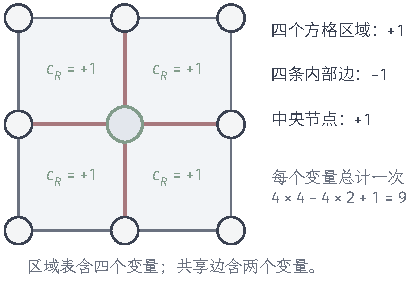
\includegraphics[width=70.831mm]{figures/06-probabilistic-graphical-models/02-inference/tikz/pgm-variational-regions/figure.pdf}
  \caption{四方格区域近似的计数。浅色块表示四个计数为$+1$的四变量区域，粗线标出四个计数为$-1$的共享内部边区域，中央节点区域的计数为$+1$。外边界线是原网格边，不表示本构造额外维护了外边界区域。每条区域一致性约束都要求大表格向子区域边缘化后与小表格相同；颜色之外还用区域面积、线条和节点区分三个层次。}
  \label{fig:pgm-variational-regions}
\end{figure}

区域消息可以由自由能的约束驻点条件导出。对约束$\sum_{\bm z_{R\setminus S}}b_R-b_S=0$引入乘子$\lambda_{R,S}(\bm z_S)$。对某张$b_R$求导时，$R$作为父区域产生正的出边乘子，作为子区域产生负的入边乘子；将它们移到等式右侧，内部驻点满足
\begin{equation}
  c_R(\log b_R-\Theta_R)
    =\sum_{P:\,P\to R}\lambda_{P,R}
       -\sum_{S:\,R\to S}\lambda_{R,S}+\text{常数}.
  \label{eq:pgm-variational-region-stationarity}
\end{equation}
归一化项及$c_R$带来的常数已经合并。每个乘子都是子区域配置上的函数，用来协调父、子两张表；因此它的指数可以作为正的校正因子。不过，直接指数化这里的$\lambda_{R,S}$，通常不能得到下面标准父子形式中的同名边消息，因为驻点方程还含$c_R$，同一约束也可能有冗余表示。需要先把一致性约束重新组合，再给新乘子取指数。消息以整个子区域的配置为索引，负计数区域的校正还会在更新中产生分母，计算对象因此比单节点消息更大。$c_R=0$时，上式只给出乘子之间的约束，不能除以$c_R$来求$b_R$；这一约束及原有的边缘一致性都应保留。

为说明计数怎样进入这种重组，记$\mathcal A(R)$为$R$的严格祖先集合，$b_A^{\downarrow S}$为将$b_A$向$S$边缘化所得的表。对一条父子边$P\to S$，考察加权约束
\begin{equation}
  G_{P,S}:=c_Sb_S+
    \sum_{A\in\mathcal A(S)\setminus(\{P\}\cup\mathcal A(P))}
         c_A b_A^{\downarrow S}=0.
  \label{eq:pgm-variational-region-weighted-constraint}
\end{equation}
原有的逐边一致性保证其中每张祖先表都边缘化为$b_S$。又因为区域及其全部祖先的计数之和为$1$，将$S$与$P$的这两个计数恒等式相减，便得
\[
  c_S+
    \sum_{A\in\mathcal A(S)\setminus(\{P\}\cup\mathcal A(P))}
      c_A=0.
\]
因此$G_{P,S}=0$确实是原一致性约束的线性组合。在四方格例中，边区域$S=e_{A,B}$只有两个祖先$A,B$，而$c_S=-1,c_A=c_B=1$，所以$G_{A,S}=0$就是$-b_S+b_B^{\downarrow S}=0$，$G_{B,S}=0$则是$-b_S+b_A^{\downarrow S}=0$。两条约束交换了原来分别协调的父区域，负计数已包含在这个组合中。

在当前四方格这种所有保留区域计数均非零的有效构造中，还能反向恢复原一致性。具体地，从最大区域向下归纳，设当前子区域$S$上方的表已经一致，记$v_S=c_Sb_S+\sum_{A\in\mathcal A(S)}c_A b_A^{\downarrow S}$。对任一父区域$P$，$P$及其祖先的计数和为$1$，而相应表已与$b_P$一致，所以$G_{P,S}=0$给出$v_S=b_P^{\downarrow S}$。各父表在$S$上的边缘因而相同，所有祖先的边缘也都等于$v_S$。将这一结果代回$v_S$的定义，得到$v_S=c_Sb_S+(1-c_S)v_S$；由$c_S\ne0$即得$b_S=v_S=b_P^{\downarrow S}$。重组约束因而不改变这些表所需满足的边缘关系。

为把这些约束写成消息，记$\mathcal D(R)$为$R$及其全部后代，$\partial R$为所有从$\mathcal D(R)$外进入$\mathcal D(R)$的有向区域边。在每个子区域配置上，以$-\xi_{P,S}(\bm z_S)$作为$G_{P,S}=0$的乘子。一个$G_{P,S}$含$b_R$，恰好意味着$S=R$，或$S$是$R$的后代而$P$在$\mathcal D(R)$外；其中$b_R$的系数都是$c_R$。因此，对非零计数区域$R$求导，约束项的贡献为$-c_R\sum_{(P\to S)\in\partial R}\xi_{P,S}$，既包括进入$R$的边，也包括从外部进入其后代的边。将它与自由能导数合并并除以$c_R$，驻点条件就写成$\log b_R=\Theta_R+\sum_{\partial R}\xi_{P,S}+\text{常数}$。取$m_{P\to S}=e^{\xi_{P,S}}$，才得到下面的边界消息表示。

含零计数区域时，上面的反推步骤不能除以$c_S$，加权约束也可能退化，故仍须保留原父子一致性，并由父表边缘确定这些区域的表；有多个父区域时，还要检查它们给出的边缘相同。不能从一条除以零的驻点式定义零计数表。一般有效区域图的父子参数化与驻点关系见Yedidia等人\scite{pgm-variational-yedidia2005}。

在标准父子区域参数化中，还能把消息方程写成可直接计算的形式。令$\Psi_R=e^{\Theta_R}$，伪边缘写为
\[
  b_R(\bm z_R)\propto
    \Psi_R(\bm z_R)
       \prod_{(P\to Q)\in\partial R}m_{P\to Q}(\bm z_Q).
\]

这里$\partial R$中的每条边都终止于$R$或其某个子区域，故相应消息只依赖$\bm z_R$内的变量。例如，四方格区域图只连接方格到其内部边、内部边到中央点。对$R=A$及$S=e_{A,B}$，后代集合及外部入边分别为
\[
  \begin{aligned}
    \mathcal D(A)&=\{A,e_{A,B},e_{A,C},o\},\\
    \partial A&=\{B\to e_{A,B},\ C\to e_{A,C},\\
              &\qquad e_{B,D}\to o,\ e_{C,D}\to o\},\\
    \mathcal D(S)&=\{S,o\},\\
    \partial S&=\{A\to S,\ B\to S,\ e_{A,C}\to o,\\
              &\qquad e_{B,D}\to o,\ e_{C,D}\to o\}.
  \end{aligned}
\]
例如$e_{B,D}\to o$进入了$A$的后代中央点，虽然没有直接进入$A$，仍须出现在$b_A$中。这些入边组合承担了计数校正，不能只保留直接指向当前区域的消息。

再把消息表示代入父子一致性。设$C_R,C_S>0$分别为两张表的归一化常数，则
\[
  \frac{1}{C_R}\sum_{\bm z_{R\setminus S}}
        \Psi_R\prod_{\partial R}m
    =\frac{1}{C_S}\Psi_S\,m_{R\to S}
        \prod_{\partial S\setminus\{R\to S\}}m.
\]
将除$m_{R\to S}$以外的子区域项移到分母，且将与$\bm z_S$无关的$C_S/C_R$吸收到消息归一化中，得到更新方程
\begin{equation}
  m_{R\to S}(\bm z_S)\propto
  \frac{\displaystyle
    \sum_{\bm z_{R\setminus S}}
      \Psi_R(\bm z_R)
       \prod_{(P\to Q)\in\partial R}m_{P\to Q}(\bm z_Q)}
  {\displaystyle
    \Psi_S(\bm z_S)
       \prod_{\substack{(P\to Q)\in\partial S\\(P\to Q)\ne(R\to S)}}
          m_{P\to Q}(\bm z_Q)}.
  \label{eq:pgm-variational-gbp}
\end{equation}

同时出现在分子、分母且只依赖$\bm z_S$的项可先约去；若还依赖被求和的变量，就不能移出求和号约去。上面的四方格例中，$m_{B\to S}$、$m_{e_{B,D}\to o}$及$m_{e_{C,D}\to o}$在两边公共，且都只依赖$S$内的变量，所以更新可化为
\[
  m_{A\to S}(\bm z_S)\propto
     \frac{\displaystyle\sum_{\bm z_{A\setminus S}}
          \Psi_A(\bm z_A)
          m_{C\to e_{A,C}}(\bm z_{e_{A,C}})}
          {\Psi_S(\bm z_S)m_{e_{A,C}\to o}(z_o)}.
\]
分母中的中央点消息正是为避免重复计入其余重叠区域而保留的校正。消息用正值初始化，每次在父区域求和、在子区域上比较并归一化，然后继续更新其他区域。这就是\term{广义置信传播}（generalized belief propagation, GBP）的一种父子消息形式。这一参数化以覆盖、计数和连通条件为前提；不同冗余约束与消息规范会给出不同但相关的更新式。固定点关系和算法构造的完整论述见Yedidia等人\scite{pgm-variational-yedidia2005}。

对贯穿例子，只要把三变量三角形本身选为最大区域，就需维护$8$项的表格；区域自由能退化为整个联合分布的真实自由能，最优值恰为$-\log26$。整个三角形区域保留了例子中的全部依赖，但也需要存储完整联合表格。若每个变量有$k$个状态，大小为$r$的区域需要$k^r$项，交集一致性还带来额外存储与通信。一般图上不断加入区域未必单调改善Kikuchi目标或每个边缘的误差，因为熵近似也随区域选择改变。满足运行交集性质的精确团树等特殊区域结构，可以建立全局一致性；一般区域图的自由能凸性和GBP收敛则需要分别分析。

区域扩张同时改变伪边缘及其一致性约束；另一条路线保持成对局部多面体不变，改用树分布构造可控的熵近似。以下仍是有限离散成对模型，先设原图连通。选取一族生成树，令参与求和的每棵树$T$都有权重$\rho_T>0$且$\sum_T\rho_T=1$；没有选入的树等价于权重为$0$。为使每条原图边都参与树熵，本节所选树族覆盖全部边。记$\rho_{i,j}=\sum_{T:(i,j)\in T}\rho_T$为边$(i,j)$的出现率，即按树权重随机选一棵树时该边被选中的概率。不连通图可按各连通分量应用同一构造，或等价地使用覆盖各分量的生成森林。

此处的目标仍是累计所有配置的概率质量，因此要在期望得分之外保留熵。若给熵乘一个系数$\tau>0$，通常称为正温度的目标；当前对数配分函数采用$\tau=1$，后面的配置推断才讨论$\tau\downarrow0$时熵消失的情形。在这个口径下，\term{树重加权}（tree-reweighted, TRW）熵定义为
\begin{equation}
  \begin{aligned}
    H_{\mathrm{TRW}}(\bm b)
      &=\sum_iH(b_i)-\sum_{(i,j)\in E}\rho_{i,j}I(b_{i,j}),\\
    I(b_{i,j})
      &=\sum_{k,l}b_{i,j}(k,l)
            \log\frac{b_{i,j}(k,l)}{b_i(k)b_j(l)}.
  \end{aligned}
  \label{eq:pgm-variational-trw-entropy}
\end{equation}
这里$I$是两节点的互信息，比较同一条边的联合表$b_{i,j}$与其两个节点边缘的乘积。以三角图为例，三棵生成树各取$1/3$权重，每条边在其中两棵树中出现，故$\rho_{i,j}=2/3$；这些系数来自一个共同的树分布。

每棵树的熵为$\sum_iH(b_i)-\sum_{(i,j)\in T}I(b_{i,j})$，所以$H_{\mathrm{TRW}}$是树熵的凸组合。对任意全局$q$，给定其树边缘的最大熵树分布的熵不小于$H(q)$；逐树加权便得$H(q)\leq H_{\mathrm{TRW}}(\bm b(q))$。因此
\begin{equation}
  A(\bm{\theta})\leq
    \max_{\bm b\in\mathcal L}
       \{\langle\bm{\theta},\bm b\rangle+H_{\mathrm{TRW}}(\bm b)\}.
  \label{eq:pgm-variational-trw-partition}
\end{equation}

树熵在树的局部一致边缘上是凹函数，可由根节点熵加沿树条件熵之和看出；其凸组合仍凹。因此这是凹目标的凸约束最大化。熵上界的依据是树熵的凸组合，边出现率因此需要来自一个树分布。关于配分函数上界的原始构造见Wainwright等人\scite{pgm-variational-wainwright2005partition}。

成对图的Bethe熵将每条边的互信息减去一次。在含环图上，这组系数通常无法成为生成树分布的边出现率，因此上述树熵上界论证不适用。TRW控制的是最优配分函数目标值，其边缘误差仍需单独检查。TRW用树熵的凸组合获得可控上界，Kikuchi用更大区域加强局部依赖约束；两者改变的机制不同。

\subsubsection{基于矩匹配的近似}

\label{sec:pgm-variational-ep}

前面的平均场/Bethe都在\emph{限制变量依赖或放松一致性}，期望传播（EP）则换了一个出发点：当模型里有一两个特别难处理的因子时，先用一个好算的“替身因子”代替它，得到一个整体好算的近似$q$；然后\emph{轮流}把每个真实因子临时放回去、算出它对关键矩（均值、方差）的影响，再调整替身，使近似分布能\emph{匹配这些矩}。这个“移除替身、放回真因子、匹配矩、写回替身”的循环就是EP。除了限制变量依赖，也可以用容易计算的分布匹配目标的局部特征。若难处理的因子使完整密度的计算成本过高，可以用易计算的指数族因子替代它们。每次暂时恢复一个真实因子，计算它对重要矩的影响，再将这些矩纳入近似分布。

设目标$p(\bm z)\propto p_0(\bm z)\prod_a f_a(\bm z)$，其中$p_0$容易处理，近似取$q(\bm z)\propto p_0(\bm z)\prod_a\widetilde f_a(\bm z)$。站点$\widetilde f_a$是替代真实因子$f_a$的指数族因子，不必单独归一化。若直接将$f_a$乘入当前$q$，真实因子与它的近似替身就会同时出现，相当于重复计入同一份作用。因此先除去$\widetilde f_a$，再放回$f_a$，得到仅在这一处恢复真实因子的临时分布。计算这个分布的均值、方差等所需矩，再寻找能够复现这些矩的近似分布，最后将修正写回站点。\term{期望传播}（expectation propagation, EP）依次在各站点重复这一过程；下面四行分别对应移除、恢复、投影和写回：
\begin{equation}
  \begin{aligned}
    q^{\setminus a}(\bm z)&\propto q(\bm z)/\widetilde f_a(\bm z),\\
    \widehat p_a(\bm z)&=
       \frac{f_a(\bm z)q^{\setminus a}(\bm z)}{Z_a},\\
    q^{\mathrm{new}}&=
       \argmin_{q'\in\mathcal Q}
           \operatorname{KL}(\widehat p_a\Vert q'),\\
    \widetilde f_a^{\mathrm{new}}(\bm z)&\propto
       q^{\mathrm{new}}(\bm z)/q^{\setminus a}(\bm z).
  \end{aligned}
  \label{eq:pgm-variational-ep}
\end{equation}
移除当前近似站点后的$q^{\setminus a}$称为\term{空腔分布}（cavity distribution），它避免同一因子被重复计算；放回真实因子得到的$\widehat p_a$称为\term{倾斜分布}（tilted distribution）。这一更新要求空腔与倾斜分布可归一化，所匹配的矩存在。$Z_a$归一化的是本次倾斜分布。第三行的有限KL投影还要求支持相容、至少一个候选的KL有限，以及最小值在候选族中取得。

具体地，设$q'_{\bm{\lambda}}=h\exp\{\langle\bm{\lambda},\bm T\rangle-A_q(\bm{\lambda})\}$具有固定支持，$\widehat p_a$不在$h=0$处放置质量，$\mathbb E_{\widehat p_a}\lVert\bm T\rVert_2<\infty$。选取一个满足$\operatorname{KL}(\widehat p_a\Vert q'_{\bm{\lambda}_0})<\infty$的候选，便有
\[
  \begin{aligned}
    \operatorname{KL}(\widehat p_a\Vert q'_{\bm{\lambda}})
      ={}&\operatorname{KL}(\widehat p_a\Vert q'_{\bm{\lambda}_0})\\
       &+A_q(\bm{\lambda})-A_q(\bm{\lambda}_0)\\
       &-\langle\bm{\lambda}-\bm{\lambda}_0,
                  \mathbb E_{\widehat p_a}\bm T\rangle.
  \end{aligned}
\]
有限矩使两个候选的对数密度比可积，因此该差值表示可由有限KL候选推得。

在自然参数域内部，按式~\eqref{eq:pgm-variational-moments}对目标求导，得到
\begin{equation}
  \mathbb E_{q^{\mathrm{new}}}\bm T
     =\mathbb E_{\widehat p_a}\bm T.
  \label{eq:pgm-variational-moment-matching}
\end{equation}
在这些有限KL条件下，投影才等价于矩匹配。若目标矩在正则最小指数族的内部均值域中，严格凸性给出唯一的投影参数；若落在边界，可能只能取极限。

矩存在且可实现时，式~\eqref{eq:pgm-variational-moment-matching}可以定义矩匹配更新。若全部候选的KL均为无穷大，该更新仍有矩匹配含义，却缺少有限KL投影解释；矩不存在时，更新本身也无定义。对高斯族，充分统计量是$\bm z$及$\bm z\bm z^\top$，故需匹配均值和协方差。

一维例子可完整算出一次更新。令$p_0(z)=\mathcal N(z;0,1)$，只有一个因子$f(z)=\mathbb I[z\geq0]$，初始近似站点为$1$。此时$q=p_0$，除去常数站点后的空腔仍是标准正态。记其密度为$\varphi(z)=(2\pi)^{-1/2}e^{-z^2/2}$，放回真实因子便将它截在非负半轴上；由对称性，半轴质量$Z_a=\int_0^\infty\varphi(z)\,dz=1/2$，故倾斜密度为$2\varphi(z)\mathbb I[z\geq0]$，即半正态分布。在它的支持上，与标准正态的密度比恒为$2$，所以两者的KL为$\log2<\infty$，满足上述有限性条件。

为求投影高斯，需要先计算两个矩。由$\varphi'(z)=-z\varphi(z)$，有$\int_0^\infty z\varphi(z)\,dz=\varphi(0)$，所以倾斜分布的均值为$2\varphi(0)=\sqrt{2/\pi}$。标准正态的$z^2\varphi(z)$是偶函数，全空间积分为$1$，因此半轴积分为$1/2$，倾斜分布的二阶矩恰为$1$。从二阶矩减去均值平方，得到
\[
  Z_a=\frac12,\qquad
  \mathbb E_{\widehat p_a}Z=\sqrt{\frac2\pi},\qquad
  \operatorname{Var}_{\widehat p_a}(Z)=1-\frac2\pi.
\]
于是$q^{\mathrm{new}}=\mathcal N(m,v)$，$m\approx0.797885$、$v\approx0.363380$。写回站点要用新高斯除以空腔。两者的对数密度分别含$-z^2/(2v)+(m/v)z$和$-z^2/2$，相减后得
\[
  \log\widetilde f_a^{\mathrm{new}}(z)
      =-\frac12(v^{-1}-1)z^2+\frac{m}{v}z+\text{常数}.
\]
若高斯自然参数写成$\eta z-\tau z^2/2$，新站点参数因此为$\tau_a=v^{-1}-1$、$\eta_a=m/v$。站点与空腔重新相乘，恰好恢复投影所得的$q^{\mathrm{new}}$。该高斯匹配均值和方差，同时在$z<0$处保留正概率。将它用于反向$\operatorname{KL}(q\Vert p)$时，目标的硬支持使KL为无穷大。矩匹配与反向KL由此对支持施加了不同要求。

EP每次投影的$\widehat p_a$依赖其他近似站点，所以其局部投影目标也随迭代变化。固定点可以与特定自由能的驻点联系起来，普通站点更新的单调性和收敛性则需要另外分析。高斯站点是不归一化的指数族因子，其精度允许为负；总体$q$以及实际使用的空腔和倾斜分布仍需合法。计算中可以采用自然参数阻尼，并检查协方差正定性和矩匹配残差。EP的站点替换与矩匹配构造来自Minka\scite{pgm-variational-minka2001}。

\subsubsection{基于局部曲率的近似}

\label{sec:pgm-variational-laplace}

对连续后验，还有一个最简单直观的近似：如果后验的质量主要集中在一个光滑的峰附近，那它在峰附近看起来就很像一个高斯——只需知道\emph{峰在哪里}（众数）和\emph{峰有多陡}（众数处的曲率，即负Hessian），就能完全确定这个高斯。拉普拉斯近似因此不需要迭代积分，只要做一次优化求众数、再算一次二阶导数。与逐因子修正的EP并行，若连续后验的主要质量集中在一个光滑峰附近，可以直接近似整个对数密度的局部形状。\term{拉普拉斯近似}（Laplace approximation）在众数附近作二阶展开，用峰的位置和曲率决定一个高斯。令$\ell(\bm z)=\log p(\bm x,\bm z)$，$\widehat{\bm z}$是内部严格局部极大点，且$\bm H=-\nabla^2\ell(\widehat{\bm z})$正定，则
\begin{equation}
  \begin{aligned}
    \ell(\bm z)&\approx\ell(\widehat{\bm z})
       -\frac12(\bm z-\widehat{\bm z})^\top
                  \bm H(\bm z-\widehat{\bm z}),\\
    q_{\mathrm L}(\bm z)&=\mathcal N(\widehat{\bm z},\bm H^{-1}),\\
    p(\bm x)&\approx
       e^{\ell(\widehat{\bm z})}(2\pi)^{d/2}|\bm H|^{-1/2}.
  \end{aligned}
  \label{eq:pgm-variational-laplace}
\end{equation}
线性项因众数处梯度为零而消失，高斯积分产生行列式项。计算上需要求众数、计算Hessian，再用Cholesky分解求解线性系统及对数行列式，不必显式求逆。负Hessian存在零方向或负方向时，上述协方差无法定义。强制正定的曲率修正可以得到其他高斯近似，但已改变原始二阶展开。

以Gamma密度$p(z)\propto z^{a-1}e^{-bz}$、$z>0$为例，取$a>1,b>0$。与$z$有关的对数密度为$\ell(z)=(a-1)\log z-bz+\text{常数}$，其两阶导数为
\[
  \ell'(z)=\frac{a-1}{z}-b,\qquad
  \ell''(z)=-\frac{a-1}{z^2}.
\]
令一阶导数为零，得到内部众数$\widehat z=(a-1)/b$；代入负二阶导数，得$-\ell''(\widehat z)=b^2/(a-1)>0$，取倒数便是近似方差。因此拉普拉斯近似为$\mathcal N((a-1)/b,(a-1)/b^2)$。当$a=3,b=1$时，它的均值、方差为$2,2$，而Gamma真实值分别为$a/b=3$、$a/b^2=3$。记标准正态分布函数为$\Phi$，近似高斯落在非法负半轴的质量为$\Phi((0-2)/\sqrt2)=\Phi(-\sqrt2)\approx7.865\%$。这里的偏差来自众数不等于均值、曲率不等于整体方差，以及二阶展开没有保留支持边界。

若改用$y=\log z$，则$z=e^y$且$dz/dy=e^y$，必须把Jacobian计入新坐标的密度：
\[
  p_Y(y)=p_Z(e^y)e^y
       \propto e^{(a-1)y-be^y}e^y
       =\exp(ay-be^y).
\]
正是Jacobian的$e^y$将对数密度中$y$的系数从$a-1$改为$a$。新对数密度的一阶导数为$a-be^y$，二阶导数为$-be^y$，故众数为$\widehat y=\log(a/b)$，众数处负曲率为$a$，近似为$Y\sim\mathcal N(\log(a/b),1/a)$。变回$Z=e^Y$便得到对数正态近似，保证正支持，却不等于直接在$z$坐标中得到的高斯。因此，拉普拉斯近似依赖展开所用的坐标；保留Jacobian后，坐标变换同时改变近似的形状和支持。

局部二阶展开近似整个积分，还需要主峰支配和尾部可控。若$\ell_n$随样本量$n$集中，唯一主峰附近的曲率按$n$增长，且高阶导数与尾部满足相应正则性，拉普拉斯法可给出渐近展开。有限样本误差则取决于峰外质量、偏斜和尾部等性质。单个高斯会遗漏其他模态；将多个峰的贡献相加时，需要找到相关峰并避免重复计数。拉普拉斯法依据局部曲率构造近似，一般没有ELBO最优性或证据上下界保证\scite{bishop2006}。

\subsection{近似的计算}
\label{sec:pgm-variational-stochastic-amortized}
\label{sec:pgm-variational-complexity}

\label{sec:pgm-variational-scalable}
选定近似族后，还要把更新公式变成可执行的计算，需处理四类问题：平均场坐标更新中的期望何时能\emph{闭式}算出（条件共轭，对应VMP）；全局参数每更新一次都要\emph{遍历全部}$n$个样本时如何降低成本（小批量的随机变分推断SVI）；ELBO中的期望积不出来时梯度如何估计（重参数化与分数函数两种梯度）；每来一个新样本都重新优化后验过于重复时如何复用（摊销推断，用共享网络一次给出后验）。下面先利用局部结构计算更新，再降低数据遍历成本，随后处理难解期望的梯度，最后减少新观测的重复优化；满足各自条件时，这些方法可以组合使用。

\subsubsection{计算局部更新}

\label{sec:pgm-variational-coordinate-vmp}
\label{sec:pgm-variational-vmp}

式~\eqref{eq:pgm-variational-coordinate}虽然形式简洁，指数中的期望仍可能难算。若完整条件分布属于指数族，
\[
  \log p(z_i\mid\bm{z}_{-i},\bm{x})
    =\log h_i(z_i)
      +\langle\bm{\eta}_i(\bm{z}_{-i},\bm{x}),\bm T_i(z_i)\rangle
      +c(\bm{z}_{-i},\bm{x}),
\]
且相关期望存在，则更新后的$q_i$保持同一家族，自然参数为
\begin{equation}
  \bm{\lambda}_i
    =\mathbb E_{q_{-i}}\bm{\eta}_i(\bm{Z}_{-i},\bm{x}).
  \label{eq:pgm-variational-conjugacy}
\end{equation}
这一结论可直接从坐标更新看出。完整条件分布与联合分布的对数只相差一个不依赖$z_i$的项，代回式~\eqref{eq:pgm-variational-coordinate}后，便得到
\[
  \log q_i^{\mathrm{new}}(z_i)
    =\log h_i(z_i)
      +\left\langle\mathbb E_{q_{-i}}\bm\eta_i,
                       \bm T_i(z_i)\right\rangle+c_i^{\mathrm{norm}},
\]
其中$c_i^{\mathrm{norm}}$只负责归一化。因此，取期望改变的是$\bm T_i$前面的自然参数，不改变关于$z_i$的函数形式。这就是条件共轭带来的计算闭合。这里不要求$\bm{\eta}_i$对其他变量线性，但必须能够计算其期望，并确认结果落在合法自然参数域内；一般不能用$\bm\eta_i(\mathbb E\bm Z_{-i},\bm x)$代替$\mathbb E\bm\eta_i(\bm Z_{-i},\bm x)$。

在因子图中，设每个邻接因子的对数中与$z_i$有关的部分能写成$\langle\bm{\eta}_{a\to i}(\bm z_{S_a\setminus\{i\}}),\bm T_i(z_i)\rangle$。把$\log h_i$只计入一次，定义消息
\[
  \bm m_{a\to i}
    =\mathbb E_{q_{S_a\setminus\{i\}}}\bm{\eta}_{a\to i},
  \qquad
  \bm{\lambda}_i=\sum_{a:\,i\in S_a}\bm m_{a\to i}.
\]
在标准共轭构造中，局部自然参数对邻居的充分统计量具有可分解的形式。例如，若某个贡献为不同邻居的$T_j(z_j)T_k(z_k)$，平均场独立性使其期望等于$\mathbb E_{q_j}T_j\,\mathbb E_{q_k}T_k$。因此变量可以把$\mathbb E_{q_i}\bm T_i$发给邻接因子，由因子组合这些期望，得到下一次所需的自然参数消息。这里需要检查的是这些统计量是否足以完成当前期望计算。若$\bm\eta_{a\to i}$包含未被所传统计量覆盖的非线性函数，就还需计算相应的高阶矩，或根据已知的$q_j$形式进行额外积分；只发送均值不会自动使任意非线性期望可算。

\term{变分消息传递}（variational message passing, VMP）就是这种利用局部结构、以所需充分统计量和自然参数交换实现坐标优化的方式。消息不必是归一化概率表，也不同于和积算法对原因子先乘后求和的消息。闭式VMP利用所选因子化及条件共轭求出期望；非共轭模型则需结合局部界、数值积分或梯度更新完成这一计算\scite{pgm-variational-winn2005}。

例如，全局成功率$\Pi\sim\operatorname{Beta}(a_0,b_0)$，$Z_i\mid\Pi\sim\operatorname{Bernoulli}(\Pi)$，观测因子为$p(x_i\mid z_i)$。取$q(\pi)\prod_iq_i(z_i)$，记$r_i=q_i(Z_i=1)$。先更新$q(\pi)$，与$\pi$有关的期望对数联合项为
\[
  \left(a_0-1+\sum_i r_i\right)\log\pi
   +\left(b_0-1+\sum_i(1-r_i)\right)\log(1-\pi).
\]
这正是Beta密度的两个对数项，说明成功与失败的整数计数被软计数替代。再更新$q_i$时，把$z_i=1$与$z_i=0$的期望对数得分相减，先验部分给出$\mathbb E\log\Pi-\mathbb E\log(1-\Pi)$，观测部分给出对数似然比。因此
\begin{equation}
  \begin{aligned}
    q(\pi)&=\operatorname{Beta}(a,b),\\
    a&=a_0+\sum_i r_i,\qquad
    b=b_0+\sum_i(1-r_i),\\
    \log\frac{r_i}{1-r_i}
      &=\mathbb E_q\log\Pi-\mathbb E_q\log(1-\Pi)
         +\log\frac{p(x_i\mid1)}{p(x_i\mid0)}.
  \end{aligned}
  \label{eq:pgm-variational-beta-bernoulli}
\end{equation}
其中$\mathbb E\log\Pi=\psi(a)-\psi(a+b)$、$\mathbb E\log(1-\Pi)=\psi(b)-\psi(a+b)$，$\psi(u)=d\log\Gamma(u)/du$是双伽马函数。局部变量向全局因子发送的是软计数$(r_i,1-r_i)$，全局变量返回的是期望对数概率，而不是$\log\mathbb E\Pi$。

取$a_0=b_0=1$，两个样本的似然比分别为$4$和$1/4$。从$q(\pi)=\operatorname{Beta}(1,1)$开始，局部更新给出$r_1=0.8,r_2=0.2$；全局更新得到$\operatorname{Beta}(2,2)$。由于新的两个期望对数概率仍相等，再次局部更新不变。这次更新通过两个软计数和两个期望完成，避免枚举$(Z_1,Z_2,\Pi)$的联合状态。相应的表达代价是$q$将$\Pi$与各$Z_i$独立化，丢失它们的后验相关性。

近似方法的单轮成本取决于需要存储和更新的局部对象。设有限离散成对图有$d$个节点、$m$条边，每节点至多$k$个状态。存储一般的稠密边势需$O(mk^2)$。一次完全平均场扫描在直接计算全部边期望时通常需$O(mk^2)$，变分边缘本身只需$O(dk)$空间；Ising等特殊代数结构可以更快。一次成对LBP扫描也通常需$O(mk^2)$，但需要$O(mk)$条目保存有向消息，若显式保存边伪边缘则另需$O(mk^2)$。在这一稠密成对设定下，两者单轮成本量级相近；总成本还取决于迭代轮数，近似误差还取决于所保留的依赖。

对于作用域$S_a$的稠密高阶因子，单次朴素局部求和本身就可能涉及$k^{|S_a|}$个配置。VMP可利用充分统计量期望的简洁形式减少枚举，其实际代价取决于这些期望的计算方式。块变分若内部树宽为$w$，表格推断通常带有$k^{w+1}$因子；Kikuchi最大区域有$r$个变量时，至少要面对$k^r$级区域表。区域方法的通信按交集状态数增长，增加区域既增加局部成本，也增加一致性校正工作。

连续近似的瓶颈常在矩阵运算。一个$d$维稠密高斯的协方差需要$O(d^2)$空间，通用Cholesky分解需$O(d^3)$时间；拉普拉斯近似与高斯EP都可能遇到它。稀疏精度、低秩更新、分块或对角表示能改变实际代价，但也可能改变近似族。EP若每个站点作用于低维投影，可局部计算倾斜矩并利用低秩更新；此时一次站点替换的代价由局部矩计算和低秩更新决定。

\subsubsection{降低数据遍历成本}

\label{sec:pgm-variational-svi}

即使每个局部更新便宜，遍历全部$n$个样本才能改变一次全局参数，也会拖慢大数据推断。设全局潜变量为$\bm u$，样本局部潜变量为$\bm z_i$，
\[
  p(\bm u,\bm z_{1:n},\bm x_{1:n})
    =p(\bm u)\prod_{i=1}^n p(\bm x_i,\bm z_i\mid\bm u),
  \qquad
  q=q_{\bm{\lambda}}(\bm u)\prod_iq_{\bm{\phi}_i}(\bm z_i).
\]
假设共轭使全局完整条件分布的自然参数等于$\bm{\lambda}_0+\sum_i\bm s(\bm x_i,\bm z_i)$。其中$\bm\lambda_0$来自先验，$\bm s_i=\bm s(\bm x_i,\bm z_i)$是第$i$个样本对全局参数的统计量贡献。固定局部因子时，最优全局自然参数为$\bm{\lambda}^\star=\bm{\lambda}_0+\sum_i\mathbb E_{q_i}\bm s_i$。

这个最优参数还给出一个适合随机更新的方向。为看清方向的来源，把全局近似写为
\[
  \log q_{\bm\lambda}(\bm u)
    =\log h(\bm u)+\langle\bm\lambda,\bm T(\bm u)\rangle
       -A_q(\bm\lambda).
\]
在固定局部因子后，期望对数联合分布中依赖$\bm u$的项具有同一基准项$\log h$，其统计量系数为$\bm\lambda^\star$。两者相减时，基准项抵消，且$\mathbb E_{q_{\bm\lambda}}\bm T=\nabla A_q(\bm\lambda)$，于是全局ELBO中依赖$\bm{\lambda}$的部分为
\[
  \mathcal L(\bm\lambda)
    =\langle\bm{\lambda}^\star-\bm{\lambda},
            \nabla A_q(\bm{\lambda})\rangle+A_q(\bm{\lambda})+C,
\]
其中$C$不依赖当前全局参数。对内积使用乘积求导，得到
\[
  \begin{aligned}
    \nabla_{\bm\lambda}\mathcal L
      &=-\nabla A_q(\bm\lambda)
        +\nabla^2 A_q(\bm\lambda)(\bm\lambda^\star-\bm\lambda)
        +\nabla A_q(\bm\lambda)\\
      &=\nabla^2 A_q(\bm\lambda)(\bm\lambda^\star-\bm\lambda).
  \end{aligned}
\]
两个一阶矩项抵消，剩下的Hessian来自矩对参数的变化率。

普通欧氏梯度以参数坐标的距离衡量更新大小，但相同长度的参数改动，可能引起不同程度的分布变化。在最小、正则指数族的自然参数域内部，Fisher信息矩阵为$\bm F(\bm\lambda)=\nabla^2 A_q(\bm\lambda)$，且正定。对于足够小的参数改动$\Delta\bm\lambda$，局部KL的二阶项为$\tfrac12\Delta\bm\lambda^\top\bm F(\bm\lambda)\Delta\bm\lambda$，所以$\bm F$给出了分布变化的局部尺度。\term{自然梯度}（natural gradient）采用$\widetilde\nabla\mathcal L=\bm F^{-1}\nabla\mathcal L$，按这一尺度校正欧氏梯度。将刚才的普通梯度代入，$\bm F^{-1}$与Hessian抵消，从而
\begin{equation}
  \widetilde\nabla_{\bm{\lambda}}\mathcal L
    =\bm{\lambda}_0+\sum_i\mathbb E_{q_i}\bm s_i-\bm{\lambda}.
  \label{eq:pgm-variational-natural-gradient}
\end{equation}
式~\eqref{eq:pgm-variational-natural-gradient}先对固定局部因子的ELBO成立。若局部因子在其参数域内部达到给定全局参数下的光滑最优值，且局部最优解及优化后的目标满足相应可微条件，包络定理允许用同一偏导计算优化掉局部变量后的目标梯度。其原因是局部最优点处关于局部参数的一阶变化为零，链式求导中由局部解随全局参数移动而产生的项随之消失；局部最优解位于约束边界、解不唯一或最优点处不可微时，需要核对相应的一阶条件与包络条件，不能直接沿用内部驻点处梯度为零的解释。

均匀抽取大小为$b$的小批量$B$，更新其中局部因子后，用
\begin{equation}
  \begin{aligned}
    \widehat{\bm{\lambda}}
      &=\bm{\lambda}_0+\frac{n}{b}
           \sum_{i\in B}\mathbb E_{q_i}\bm s_i,\\
    \bm{\lambda}^{(t)}
      &=(1-\rho_t)\bm{\lambda}^{(t-1)}
          +\rho_t\widehat{\bm{\lambda}}
  \end{aligned}
  \label{eq:pgm-variational-svi}
\end{equation}
构造\term{随机变分推断}（stochastic variational inference, SVI）的全局更新。这里还要保证每一步仍对应合法分布。记$\Omega=\operatorname{int}\{\bm\lambda:A_q(\bm\lambda)<\infty\}$为当前正则族所用的自然参数域，并选取$\bm\lambda^{(0)}\in\Omega$。指数族的自然参数域是凸的；若本批目标$\widehat{\bm\lambda}\in\Omega$，且$0<\rho_t\leq1$，上式便是域内两点的凸组合，因而仍在$\Omega$内。小批量缩放后的目标是否在域内，需要由具体共轭模型确认；若不满足，不能直接使用该次更新，应修正目标的构造或采用另外有合法性保证的更新。对于非凸的其他约束，还需检查这些约束本身。步长大于$1$会变成外推，即使两个端点都合法，也不保证新参数合法。

在给定当前全局参数并精确求解相应局部问题时，缩放的统计量和是全数据和的无偏估计。非均匀抽样需要按纳入概率加权；局部问题未充分求解时，估计中还包含局部优化误差，精确局部解下的无偏结论需要相应调整\scite{pgm-variational-hoffman2013}。

在式~\eqref{eq:pgm-variational-beta-bernoulli}中，若$n=1000$，抽到的$10$个样本的$r_i$之和为$7$，先验仍为$\operatorname{Beta}(1,1)$，则小批量给出的目标分布是$\operatorname{Beta}(701,301)$。若当前分布为$\operatorname{Beta}(501,501)$，取步长$0.1$，更新为$\operatorname{Beta}(521,481)$。缩放发生在统计量而不是先验上，否则会把先验重复计算。

随机更新以有噪声的小批量方向替代全数据方向，因此单步ELBO可能下降。在保持上述每步合法性的基础上，常用递减步长还满足$\sum_t\rho_t=\infty$、$\sum_t\rho_t^2<\infty$。例如，从$t=1$起取$\rho_t=(t+t_0)^{-\kappa}$，其中$t_0\geq0$、$1/2<\kappa\leq1$，就同时有$0<\rho_t\leq1$与这两个和式条件。式~\eqref{eq:pgm-variational-svi}中的当前参数因此记为$\bm\lambda^{(t-1)}$，更新后记为$\bm\lambda^{(t)}$。和式条件约束长期累计的更新及噪声，并不能代替参数域检查。在光滑性、迭代有界、噪声矩受控等随机逼近条件下，可以分析迭代趋向驻点的行为。局部计算解释当前批次的样本，全局计算汇总缩放后的统计量，这一分工使每次更新只需读取部分数据。

SVI将每次全数据局部计算从$n$个样本改为$b$个样本，代价约为$bC_{\mathrm{local}}+C_{\mathrm{global}}$，其中两项分别是单样本局部更新和全局更新成本。若无需保留所有局部因子，还可避免$O(n)$份局部状态存储；总训练成本仍取决于达到目标精度所需的小批量数。

近似族的选择取决于需要估计的量。主要计算单变量边缘且内存有限时，完全平均场提供成本较低的起点；其遗漏的相关性仍可能影响这些边缘。若查询涉及相邻状态的联合概率或整段轨迹，保留链或小块依赖能直接表达所需的联合事件，代价是块内推断。是否增加结构，需要比较相关查询的误差和计算成本。

计算方式可以叠加在选定的近似族上。条件共轭且统计量期望可算时，VMP组织解析更新；模型还具有可分解的局部统计量和全局更新时，SVI通过小批量减少一次遍历的数据量。例如，每个样本是一段序列时，可在$q_{\bm\phi_i}(\bm z_i)$中保留整条链，精确计算链内统计量，再用小批量更新共轭的全局参数。这一组合同时保留局部结构并降低数据遍历成本，单条链内部的推断复杂度仍由链的模型决定。

\subsubsection{估计难解期望的梯度}
\label{sec:pgm-variational-gradient-estimation}

小批量抽样减少了需要处理的数据量，但每个样本的ELBO仍可能包含无法解析计算的期望。非共轭模型中，局部更新因而常需改为梯度优化，并通过潜变量采样估计梯度。困难在于：改变近似参数时，$q$既改变被平均的函数，也改变样本落在哪里。若把已经抽到的样本当成固定输入，只对函数求导，就可能漏掉分布变化的影响。为了保留这一影响，可以先抽取分布固定的噪声，再把噪声变换为$q$的样本；改变参数时，沿同一份噪声追踪样本位置的变化。对于能够写成$\bm z=g_{\bm{\phi}}(\bm\epsilon)$、$\bm\epsilon\sim r(\bm\epsilon)$且$r$不依赖$\bm{\phi}$的分布，随机性可以与参数分开。例如高斯分布可写为$\bm z=\bm m+\bm L\bm\epsilon$，$\bm\epsilon\sim\mathcal N(\bm0,\bm I)$，$\bm L\bm L^\top$为协方差。令$F_{\bm{\phi}}(\bm z)=\log p(\bm x,\bm z)-\log q_{\bm{\phi}}(\bm z)$，当$g_{\bm\phi}$和$F_{\bm\phi}$在所需参数与样本处可微，且链式导数满足可交换微分与期望的可积支配条件时，
\begin{equation}
  \begin{aligned}
    \nabla_{\bm{\phi}}\mathcal L
      =\mathbb E_r\big[
        &(\nabla_{\bm{\phi}}g_{\bm{\phi}})^\top
           \nabla_{\bm z}F_{\bm{\phi}}
                (g_{\bm{\phi}}(\bm\epsilon))\\
        &+\left.\nabla_{\bm{\phi}}F_{\bm{\phi}}(\bm z)
          \right|_{\bm z=g_{\bm{\phi}}(\bm\epsilon)}
        \big].
  \end{aligned}
  \label{eq:pgm-variational-pathwise}
\end{equation}
第二行对$\bm z$保持固定，只微分$F$的显式参数依赖；第一行则跟踪样本位置随参数移动的影响。这是\term{重参数化梯度}（reparameterization gradient），也称路径导数估计：先把期望写到固定噪声上，再用链式法则求导。样本位置的参数依赖由第一项显式保留；模型含待学习参数时，还需计算对应的显式偏导。第~\ref{chap:pgm-generative}章将在VAE中使用这一梯度估计\scite{kingma2013}。

以$q=\mathcal N(m,s^2)$、$s>0$和$f(z)=z^2$为例，$z=m+s\epsilon$，路径导数的单样本估计分别是$2(m+s\epsilon)$与$2(m+s\epsilon)\epsilon$，期望为$2m$与$2s$，恰与$\partial_m(m^2+s^2)$、$\partial_s(m^2+s^2)$一致。这些单样本导数的期望给出正确梯度，但有限样本估计仍有方差。与其他估计器的方差比较，需要固定目标函数和分布。

离散变量的普通采样映射对参数通常是阶梯函数，几乎处处导数为零，直接套用路径导数不能得到正确梯度。另一种办法直接微分概率权重，而不追踪单个样本的位置。为使用这一办法，先假设$q_{\bm\phi}$相对于同一基准测度，在一个不随$\bm\phi$变化的支持集上为正，且$q_{\bm\phi}$与$f_{\bm\phi}$对参数可微。有限状态空间中，可在各项有限时逐项求导；对于可数无穷或连续支持，还需要允许微分与求和或积分交换。例如，在当前参数的一个邻域内，$q_{\bm\phi}f_{\bm\phi}$及$q_{\bm\phi}$的各参数偏导分别受可积函数支配，并且下面乘积求导后的两项均绝对可积，就是一组足够条件。此时，按同一测度积分，有
\[
  \begin{aligned}
    \nabla_{\bm\phi}\int q_{\bm\phi}(\bm z)f_{\bm\phi}(\bm z)\,d\bm z
      &=\int\big[(\nabla_{\bm\phi}q_{\bm\phi})f_{\bm\phi}
                   +q_{\bm\phi}\nabla_{\bm\phi}f_{\bm\phi}\big]\,d\bm z.
  \end{aligned}
\]
再在正支持集上代入$\nabla q=q\nabla\log q$，可得
\begin{equation}
  \nabla_{\bm{\phi}}\mathbb E_{q_{\bm{\phi}}}f_{\bm{\phi}}(\bm Z)
    =\mathbb E_q\!\left[
       f_{\bm{\phi}}(\bm Z)\nabla_{\bm{\phi}}\log q_{\bm{\phi}}(\bm Z)
       +\nabla_{\bm{\phi}}f_{\bm{\phi}}(\bm Z)\right].
  \label{eq:pgm-variational-score-function}
\end{equation}
这称为\term{分数函数估计}（score-function estimator），其中“分数”指对数密度对参数的导数。固定支持排除了移动积分边界的影响，可微性与求导交换条件则支持上面的乘积求导，二者承担不同职责。在同样允许对归一化等式求导的条件下，
\[
  \mathbb E_q\nabla_{\bm\phi}\log q_{\bm\phi}
    =\int\nabla_{\bm\phi}q_{\bm\phi}\,d\bm z
    =\nabla_{\bm\phi}\int q_{\bm\phi}\,d\bm z=\bm0.
\]
因此，从第一项的$f_{\bm\phi}$中减去不依赖所采变量的基线，不改变这一项的期望，却可能降低方差。若基线还依赖参数，这个结论是把它作为该梯度估计器中的系数使用，并不意味着可以把整个目标换成$f_{\bm\phi}$减基线后再忽略其显式导数。小状态空间也可以精确求和；连续松弛则用可微随机变量替代离散变量，一般改变了目标或引入偏差。支持集随参数变化时，求导还涉及积分边界，上式需要加入相应的边界处理。

\subsubsection{降低重复推断成本}

\label{sec:pgm-variational-amortized}

小批量减少了每次读取的数据，却仍需为每个新样本求解局部优化。若样本不断到来，可以学习一个共享映射$\bm{\phi}_i=f_{\bm{\omega}}(\bm x_i)$，直接输出$q_{\bm{\phi}_i}(\bm z_i)$的参数。\term{摊销推断}（amortized inference）把许多样本的推断计算转移到一次共享训练中；测试时主要执行前向计算，也可以在其输出上继续作样本级优化。

摊销推断将测试时的迭代换成网络前向计算，共享训练还需计入反向传播和模型存储。小批量SVI与摊销映射可以结合：每次只抽取一批样本，用共享映射生成它们的局部参数，再计算这一批的统计量或梯度。小批量减少每次处理的数据量，摊销映射减少每个样本单独执行的优化；网络输出若未达到局部最优，仍须保留前述局部优化误差的限制。

共享映射减少了逐样本优化，也限制了各样本的局部参数如何取值。为分解其逐样本误差，以下改用固定生成参数$\bm\theta$、样本间相互独立的局部潜变量模型，并定义局部ELBO：
\[
  \begin{aligned}
    p_{\bm\theta}(\bm x_{1:n},\bm z_{1:n})
      &=\prod_i p_{\bm\theta}(\bm x_i,\bm z_i),\\
    \mathcal L_i(\bm\phi)
      &=\mathbb E_{q_{\bm\phi}}
          \log p_{\bm\theta}(\bm x_i,\bm Z_i)+H(q_{\bm\phi}).
  \end{aligned}
\]
前面的SVI层次模型包含共享随机量$\bm u$，积分掉它通常产生样本间依赖，联合对数证据因而不能逐样本相加，其ELBO还包括全局因子的贡献。

在上述独立模型中，令$\mathcal L_i^\star=\sup_{\bm{\phi}}\mathcal L_i(\bm{\phi})$；设共享网络达到其最优参数$\bm{\omega}^\star$，实际训练结果为$\widehat{\bm{\omega}}$。假设以下各目标值有限，对同一批样本有
\begin{equation}
  \begin{aligned}
    &\sum_i\log p_{\bm\theta}(\bm x_i)
       -\sum_i\mathcal L_i(f_{\widehat{\bm{\omega}}}(\bm x_i))\\
    ={}&\sum_i[\log p_{\bm\theta}(\bm x_i)-\mathcal L_i^\star]\\
     &+\left[\sum_i\mathcal L_i^\star
          -\sum_i\mathcal L_i(f_{\bm{\omega}^\star}(\bm x_i))\right]\\
     &+\left[\sum_i\mathcal L_i(f_{\bm{\omega}^\star}(\bm x_i))
          -\sum_i\mathcal L_i(f_{\widehat{\bm{\omega}}}(\bm x_i))\right].
  \end{aligned}
  \label{eq:pgm-variational-amortization-gap}
\end{equation}
三项分别是近似族误差、共享映射限制带来的摊销误差和网络优化误差，按定义均非负。若最优值未取得，改用上确界解释。网络最优性针对同一固定模型下的样本总目标，个别样本上的ELBO可能低于实际训练结果。关于近似与摊销两类误差的区分，可参见Cremer等人的分析\scite{pgm-variational-cremer2018}。

式~\eqref{eq:pgm-variational-amortization-gap}衡量近似结果对模型后验的偏离。生成模型遗漏现实中的因素时，精确后验也可能产生失准预测，这属于模型失配。若共享训练同时调整生成参数，后验和近似族会共同变化，ELBO的改善也同时包含模型和推断两方面的变化。

\subsection{近似的可靠性}

\label{sec:pgm-variational-results-diagnostics}
\label{sec:pgm-variational-analysis}
\label{sec:pgm-variational-convergence}
\label{sec:pgm-variational-diagnostics}

近似方法给出的不是精确答案，需要判断其可靠性、误差来源以及是否影响目标查询。分布近似和配置近似的诊断方式不同：前者要检查支持是否相容、相关性是否被丢掉、能否用ELBO间隙或重要性加权给出误差界；后者要看原始--对偶间隙。诊断首先要与输出对象相符。平均场和结构化VI定义合法的全局$q$，可在其下计算联合事件，但可表达的依赖受近似族限制。Bethe和Kikuchi维护局部一致的伪边缘，联合查询还需确认这些表能否来自共同的全局分布。拉普拉斯法与高斯EP输出高斯或指数族近似，其支持、尾部和多峰结构需要与目标比较。诊断所检查的概率或期望，应与这些对象实际能回答的查询一致。

求解近似目标涉及另一层误差。精确平均场坐标更新使ELBO单调且有界，因此目标值收敛。若要进一步证明迭代点趋向驻点，还需连续性、紧的水平集、坐标子问题解的适当唯一性等条件；一般非凹的联合目标也可能有多个坐标最优点。随机变分允许单步ELBO下降，其收敛分析还需控制梯度噪声，通常得到相应条件下的渐近驻点结论。

对于LBP，我们可以先单独考察固定点的存在性。对本章有限离散、严格正的情形，记$\psi_a$的最小、最大值为$u_a>0,v_a$，$k_i=|\mathcal X_i|$。对任意正输入，归一化后的因子到变量消息都满足$m_{a\to i}(z_i)\geq u_a/(k_iv_a)$：求和中的其他消息乘积不依赖$z_i$，用$u_a$控制分子、用$k_iv_a$控制归一化分母即可。把每条消息限制在具有这一正下界的概率单纯形内，所有消息组成的集合非空、紧且凸；将变量消息代入式~\eqref{eq:pgm-variational-lbp}后，同步更新是这个集合上的连续自映射。由Brouwer不动点定理，它至少有固定点。正下界保证消息乘积及归一化有定义；若允许任意零消息，乘积可能处处为零，连续自映射的前提便可能失效。

上述证明给出至少一个固定点，但未建立它对迭代的吸引性。LBP仍可能周期振荡，局部稳定性和自由能极小性也需要分别判断。因子含零时，正下界消失，固定点存在性还需其他论证。EP固定点满足的是局部矩匹配，拉普拉斯法使用的是找到的众数与曲率；评估边缘精度仍需比较这些结果与目标分布。

表~\ref{tab:pgm-variational-objectives}按输出和目标列出各方法的界。具有界的目标值可以形成相应证书；没有一般界方向时，边缘比较、残差和其他诊断提供补充证据。
\begin{table*}[htbp]
  \centering
  \begin{tabularx}{\linewidth}{l*{3}{>{\raggedright\arraybackslash}X}}
    \toprule
    方法与输出 & 优化或匹配对象 & 可用的界 & 不由此推出的结论\\
    \midrule
    平均场、结构化VI & 合法$q$的期望得分与真实熵 & ELBO不高于对数证据 & 所有边缘及尾概率都准确\\
    Bethe、Kikuchi & 局部一致表与近似熵 & 一般没有统一上下界方向 & 固定点是全局最优或真实边缘\\
    EP & 倾斜分布的局部矩匹配 & 一般没有证据界方向 & 站点更新单调提高同一ELBO\\
    拉普拉斯近似 & 众数处对数密度的二阶展开 & 一般没有证据界方向 & 峰附近曲率控制整体分布误差\\
    配分函数TRW & 树熵上界与局部多面体 & 理论最优值不低于对数配分函数 & 每个近似边缘都更准确\\
    MPE的LP与对偶 & 配置得分的线性松弛 & 对偶值不低于最大得分 & 分数解就是可行配置\\
    \bottomrule
  \end{tabularx}
  \caption{各方法的目标与证书。分布近似的ELBO界针对对数证据；配置近似的LP界针对最大得分。二者可以使用相同的局部统计量，但对应不同的目标值。TRW行的界针对精确优化后的值；实际计算要报告经验证的上界证书，不能把尚未最优的原始可行目标直接当作上界。}
  \label{tab:pgm-variational-objectives}
\end{table*}
\FloatBarrier

分布诊断需要覆盖实际查询。单峰$q$可能遗漏目标的其他模态，独立$q$可能丢失强相关性，支持不相容还可能使反向KL为无穷大。三角图已经显示，正确的单节点边缘可以与错误的联合依赖同时出现。因此，变量组合的概率、预测尾部或相关系数等所需统计量，应直接进入检查。

对同一固定模型，提高精确ELBO等价于降低反向KL。这里继续用$\pi=p(\bm z\mid\bm x)$表示目标后验，避免与联合模型$p(\bm x,\bm z)$混淆。若能得到有限的$\varepsilon=\log p(\bm x)-\mathcal L(q)=D_{\mathrm{KL}}(q\Vert\pi)$，Pinsker不等式给出
\[
  \|q-\pi\|_{\mathrm{TV}}
    :=\sup_A|q(A)-\pi(A)|\leq\sqrt{\varepsilon/2}.
\]
这里的全变差采用事件概率差的上确界口径；有共同密度时，它等于密度差绝对值积分的一半。为把事件概率误差转为统计量误差，先考虑$0\leq g\leq1$。由$g(\bm z)=\int_0^1\mathbb I[g(\bm z)>t]\,dt$，期望差可写为这些阈值事件概率差的积分，所以$|\mathbb E_qg-\mathbb E_\pi g|\leq\|q-\pi\|_{\mathrm{TV}}$。对于值域在$[a,b]$且$a<b$的函数$f$，取$g=(f-a)/(b-a)$，便有
\[
  |\mathbb E_qf-\mathbb E_\pi f|
    \leq(b-a)\|q-\pi\|_{\mathrm{TV}}
    \leq(b-a)\sqrt{\varepsilon/2}.
\]
$a=b$时函数为常数，两边的期望差直接为零。这是误差上界，单个统计量的实际误差未必随每次ELBO更新下降。对数证据通常未知，所以ELBO绝对值本身无法确定$\varepsilon$；方差等无界统计量还需要额外矩条件。蒙特卡洛ELBO估计有采样波动，单次估计值可能高于真实对数证据；理论下界约束的是精确ELBO。

可以利用重要性权重进行补充检查。若$q(\bm z)>0$覆盖$p(\bm x,\bm z)>0$的全部区域，独立采样$\bm z^{(1)},\ldots,\bm z^{(K)}\sim q$，定义
\begin{equation}
  w_k=\frac{p(\bm x,\bm z^{(k)})}{q(\bm z^{(k)})},
  \qquad
  \widehat Z_K=\frac1K\sum_{k=1}^K w_k.
  \label{eq:pgm-variational-importance}
\end{equation}
此时$\mathbb E\widehat Z_K=p(\bm x)$，而Jensen不等式给出$\mathbb E\log\widehat Z_K\leq\log p(\bm x)$，其中允许$\log0=-\infty$。该界约束重复采样下的期望，单次$\log\widehat Z_K$仍可能高于真实值。仅当$\sum_kw_k>0$时，后验期望才可用$\sum_kw_kf(\bm z^{(k)})/\sum_kw_k$作自归一化估计；该比值通常存在有限样本偏差。一个保证其一致性的充分条件是$\mathbb E_\pi|f|<\infty$，因为支持覆盖使
\[
  \mathbb E_qw=p(\bm x)>0,
  \qquad
  \mathbb E_q|wf|=p(\bm x)\mathbb E_\pi|f|<\infty.
\]
独立同分布采样下，大数定律分别给出$K^{-1}\sum_kw_k\to p(\bm x)$与$K^{-1}\sum_kw_k\allowbreak f(\bm z^{(k)})\to p(\bm x)\allowbreak\mathbb E_\pi f$，均几乎必然成立。分母极限严格为正，所以其比值几乎必然趋于$\mathbb E_\pi f$；有限批次的分母仍可能为零。这组一阶可积条件用于一致性，尚不保证有限方差或常规标准误差。这里要求目标被$q$覆盖，与反向KL要求$q$避开目标零区域是不同方向的支持条件。

同样仅在$\sum_kw_k>0$时，才计算基于权重的\term{有效样本量}（effective sample size, ESS）
\[
  \widehat{\mathrm{ESS}}
  =\frac{(\sum_kw_k)^2}{\sum_kw_k^2}.
\]
它衡量本批权重是否集中在少数样本上，取值介于$1$与$K$之间。$K$个样本的权重相等且为正时，ESS为$K$；只有一个权重非零时，ESS为$1$。例如实际抽了四次，权重为$(9,1,0,0)$，则ESS为$10^2/(9^2+1^2)=100/82\approx1.22$。两个样本的权重非零，但主要贡献集中于其中一个，所以ESS接近$1$。它描述贡献的集中程度。

即使提议覆盖目标支持，也可能抽到全零权重批次。以前面的半正态为目标，取未归一化密度$\mathcal N(z;0,1)\mathbb I[z\geq0]$和标准正态提议，则$w_k=\mathbb I[z^{(k)}\geq0]$，全零批次的概率为$2^{-K}$。此时证据估计为$0$，自归一化比值和ESS无定义，可记录为“无有效加权样本”。计算中还需区分真实零权重与数值下溢：用对数权重检查数值范围，检查提议与目标的重叠，再决定是否增加采样量。如果把这批全零权重强行改成均匀正权重，再报告后验期望或ESS，就改变了原来由目标与提议密度比规定的加权估计，不能保留这批样本的原始权重信息。

权重集中于少数样本时，低ESS提示提议与目标重叠不足，或采样量偏少。但若整批样本都未到达某个目标模态，已观测到的权重仍可能平稳。因此，ESS检查的是本批权重的集中程度，后验统计量精度还需其他证据；权重二阶矩不存在时，常规标准误差也失去相应依据。多初值比较、小规模精确枚举、较丰富近似族，以及第~\ref{chap:pgm-sampling}章的采样诊断，可以相互补充。

\term{后验预测检查}（posterior predictive check）将推断结果接回观测模型。先从近似后验抽取潜变量或参数，再生成复制数据，比较复制数据与真实数据中有意义的统计量。若某种结构未被复现，问题可能来自模型失配，也可能来自推断误差。在小规模问题上改用精确推断，或对同一模型比较不同近似方法，有助于区分这两个来源\scite{pgm-murphy2012}。

\section{近似MPE}

\label{sec:pgm-variational-mpe}

\subsection{完整配置的连续松弛}

\label{sec:pgm-variational-ilp-local-polytope}
\label{sec:pgm-variational-lp}

现在转到本章第二条主线：从“求整个后验\emph{分布}”转为“求一组最可能的\emph{配置}”（MPE）。两者看似都在做优化，但有本质区别——分布推断要给所有候选配置累计概率质量（求和里带着熵），MPE则只要找出\emph{得分最高的那一个}配置（没有熵项）。一个关键的转化技巧是：离散的“选标签”可以先写成0/1指示变量、变成整数规划；再把0/1约束放松成$[0,1]$连续值，就得到一个线性规划松弛，它给出最优得分的\emph{上界}，且分数解常可借助图结构恢复成合法配置。现在将查询从后验分布转为完整配置：给定证据，为全部非证据变量选择一组联合最优值。这里采用MPE的纯最大化定义（第~\ref{sec:pgm-elimination-mpe}节）。一般边缘MAP的目标是$\max_{\bm z_Q}\log\sum_{\bm z_R}\exp S(\bm z_Q,\bm z_R)$，还包含对其余变量的求和。后文LP近似处理完整配置的最大化；保留求和的边缘MAP需要使用相应的查询与消元顺序（第~\ref{sec:pgm-elimination-map}节）。

设所有变量有限离散，证据吸收后的对数得分为
\begin{equation}
  S(\bm z)=\sum_i\theta_i(z_i)
              +\sum_a\theta_a(\bm z_{S_a}),
  \qquad M=\max_{\bm z\in D}S(\bm z).
  \label{eq:pgm-variational-mpe-score}
\end{equation}
这里的得分暂不含$-\log Z$；它不影响最优配置。先设得分有限且可行配置非空。硬约束可以通过删除禁止状态或增加显式约束表示，使后文LP的系数保持有限。下文给出的局部LP及其分解公式，先针对节点状态和因子允许配置上的归一化与局部一致性约束；可由局部因子表示的禁配状态，应从相应因子配置集中删除。若另有显式的非局部约束，也必须在LP中保留，并在分解时相应增加约束乘子或子问题，不能把这些限制随二值条件一同丢掉。

为把配置写成线性变量，对每个节点状态$k\in\mathcal X_i$引入$\delta_i(k)\in\{0,1\}$，对每个因子配置$\bm s\in\mathcal X_{S_a}$引入$\delta_a(\bm s)\in\{0,1\}$。要求
\begin{equation}
  \begin{aligned}
    &\sum_{k\in\mathcal X_i}\delta_i(k)=1,\qquad
       \sum_{\bm s\in\mathcal X_{S_a}}\delta_a(\bm s)=1,\\
    &\sum_{\bm s:\,s_i=k}\delta_a(\bm s)=\delta_i(k),
        \qquad i\in S_a.
  \end{aligned}
  \label{eq:pgm-variational-ilp-constraints}
\end{equation}
每个节点恰选一个标签，每个因子恰选一个与其节点标签相容的配置。最大化
\[
  \sum_{i,k}\theta_i(k)\delta_i(k)
     +\sum_{a,\bm s}\theta_a(\bm s)\delta_a(\bm s)
     =\langle\bm{\theta},\bm{\delta}\rangle
\]
就得到\term{整数线性规划}（integer linear programming, ILP）表示。给定$\bm z$可唯一构造这些指示变量；反过来，节点的唯一标签及一致性迫使每个因子也选中对应配置。整数可行解因此与原配置一一对应，线性目标保留原配置得分。

由于$\mathcal M$是全部配置指示向量的凸包，
\begin{equation}
  M=\max_{\bm{\mu}\in\mathcal M}
          \langle\bm{\theta},\bm{\mu}\rangle.
  \label{eq:pgm-variational-mpe-marginal}
\end{equation}
证明只需观察：凸组合的得分是配置得分的加权平均，不会高于最大配置得分，而最优配置本身就在凸包里。精确MPE由此转为连续线性优化，但描述$\mathcal M$仍需要完整的全局一致性条件。

丢掉二值要求，只保留$\mu_i,\mu_a\geq0$及式~\eqref{eq:pgm-variational-ilp-constraints}中的线性等式，就得到局部多面体$\mathcal L$上的\term{线性规划松弛}（linear programming relaxation, LP relaxation）：
\begin{equation}
  U_{\mathrm{LP}}
     =\max_{\bm{\mu}\in\mathcal L}
               \langle\bm{\theta},\bm{\mu}\rangle,
  \qquad
  S(\widehat{\bm z})\leq M\leq U_{\mathrm{LP}}.
  \label{eq:pgm-variational-lp-bound}
\end{equation}
左侧要求$\widehat{\bm z}$是真实可行配置，右侧来自$\mathcal M\subseteq\mathcal L$。若求得的LP最优解为整数，它就是全局最优配置；分数最优解给出上界及伪边缘，合法配置还需恢复。迭代中的原始可行分数解尚未达到最优值时，其目标可能低于$M$。可以用于证书的上界来自LP对偶可行解，或经验证的LP最优值。

LP近似保留原配置得分，放宽可行域，其上界直接来自集合包含关系。拉普拉斯法和EP近似的是分布形状或局部矩（第~\ref{sec:pgm-variational-laplace-ep}节）。LP的数值证书回答最大得分查询，后验概率和不确定性则需要分布推断。

三角图中，取$\mu_i(0)=\mu_i(1)=1/2$，每条边$\mu_{i,j}(0,1)=\mu_{i,j}(1,0)=1/2$，其余为$0$。这是图~\ref{fig:pgm-variational-triangle}右侧的局部一致点，得分为$3\beta$，且每条边的期望奖励至多为$\beta$，故$U_{\mathrm{LP}}=3\beta$。真实最优值只有$M=2\beta$。这个分数点要求三个二元变量两两不同，缺少对应的合法配置。增加三角不等式$\sum_{(i,j)\in E}\Pr(Z_i\ne Z_j)\leq2$即可把本例的最优值压回$2\beta$，但一般图需要哪些更高阶约束，仍是计算问题。

配置优化也可看成熵消失的极限。对$\tau>0$，有限状态空间上
\[
  \max_{\bm z}S(\bm z)
  \leq \tau\log\sum_{\bm z}e^{S(\bm z)/\tau}
  \leq \max_{\bm z}S(\bm z)+\tau\log|D|.
\]
左侧取最大的一项，右侧把每一项都用最大项控制，故$\tau\downarrow0$时夹逼到$M$。由熵对偶，中间量等于$\max_{\bm{\mu}\in\mathcal M}\{\langle\bm{\theta},\bm{\mu}\rangle+\tau H^\star(\bm{\mu})\}$。这说明分布推断与配置推断为何共享几何工具，也说明两者并非同一个查询：正温度下要计入全部配置的质量，零温度下只关心最大值。

\subsection{松弛问题的分解求解}
\label{sec:pgm-variational-decomposed-solving}

松弛后的LP变量和约束依然很多，直接喂给通用求解器不够高效。对偶分解的思路是\emph{分而治之}：把节点和因子各自看成一个容易独立求解的小问题，让共享变量在各子问题里先各拿一份副本、暂时独立地选，再用乘子反复\emph{协调}这些副本的分歧、最终达成一致。连续松弛仍可能包含大量变量和约束。将目标分到可求解的因子或树上，再协调重复变量，可以把整体求解转为局部计算，并保留用于评价配置的上界。

\subsubsection{基于因子分解的求解}

\label{sec:pgm-variational-dual-decomposition}
\label{sec:pgm-variational-dual-trw}

局部LP包含许多节点和因子变量，直接求解时还要同时维护它们的一致性。各因子自身的配置优化可能较容易，难点在于共享变量的取值协调。\term{对偶分解}（dual decomposition）为共享变量建立子问题副本，暂时分别求解，再通过乘子重分配得分，协调这些副本。

一个能直接核验的分解将每个节点和每个因子作为子问题。局部LP要求$\mu_i(k)-\sum_{\bm s:s_i=k}\mu_a(\bm s)=0$，这正是节点表与因子表对同一状态的意见一致。对每个这样的等式引入实数乘子$\lambda_{a,i}(k)$，并把它乘以等式左端加到目标中，得到Lagrangian
\[
  \begin{aligned}
    \mathscr L(\bm\mu,\bm\lambda)
      ={}&\sum_{i,k}\theta_i(k)\mu_i(k)
          +\sum_{a,\bm s}\theta_a(\bm s)\mu_a(\bm s)\\
       &+\sum_{a,i\in S_a,k}\lambda_{a,i}(k)
           \left[\mu_i(k)-\sum_{\bm s:s_i=k}\mu_a(\bm s)\right]\\
      ={}&\sum_{i,k}\left[\theta_i(k)+\sum_{a:i\in S_a}\lambda_{a,i}(k)\right]\mu_i(k)\\
       &+\sum_{a,\bm s}\left[\theta_a(\bm s)-\sum_{i\in S_a}\lambda_{a,i}(s_i)\right]\mu_a(\bm s).
  \end{aligned}
\]
最后两行分别收集每张节点表与因子表的系数，解释了同一乘子为何在节点处取正号、在因子处取负号。暂时去掉节点与因子之间的一致性，只保留各表自身的非负与归一化约束。单纯形上的线性函数是各状态系数的概率加权平均，其最大值就是最大系数，并可在相应状态的指示向量处取得。因此，对各表独立最大化$\mathscr L$，得到
\begin{equation}
  \begin{aligned}
    D(\bm{\lambda})
       ={}&\sum_i\max_{k\in\mathcal X_i}
          \left[\theta_i(k)+\sum_{a:\,i\in S_a}\lambda_{a,i}(k)\right]\\
        &+\sum_a\max_{\bm s\in\mathcal X_{S_a}}
          \left[\theta_a(\bm s)-\sum_{i\in S_a}\lambda_{a,i}(s_i)\right].
  \end{aligned}
  \label{eq:pgm-variational-dual}
\end{equation}
对任意共同配置，把同一$z_i$代入所有副本，乘子逐项抵消，子问题得分之和等于$S(\bm z)$；各子问题独立取最大只会提高这个和。因此$D(\bm{\lambda})\geq M$对任意有限乘子成立。$D$是仿射函数的最大值之和，故凸，目标是最小化这个上界。

设节点子问题选出$k_i^\star$，因子子问题选出$\bm s_a^\star$，则
\[
  g_{a,i}(k)=\mathbb I[k_i^\star=k]-\mathbb I[s_{a,i}^\star=k]
\]
是一个次梯度。具体而言，把当前选中的局部最优状态固定后，式~\eqref{eq:pgm-variational-dual}中对应的是一个关于乘子的仿射分支；$\lambda_{a,i}(k)$在该分支里的系数，正是节点指示值减因子指示值。当前分支达到最大值，它的斜率便给出凸函数$D$的一个次梯度。于是可用更新$\lambda_{a,i}^{(t+1)}(k)=\lambda_{a,i}^{(t)}(k)-\eta_t g_{a,i}(k)$。若节点选择了$k$而因子没有，更新降低节点对$k$的奖励，同时提高该因子对$k$的奖励，促使分歧缩小。平局时可选择任一最优配置，或在最优指示向量之间取凸组合。次梯度法单步不保证上界下降，实际应保留历次最小的$D$；也可使用有针对性的块坐标或平滑方法。

上述Lagrangian展开同时说明，这个上界是局部LP的对偶，而不仅是某个独立构造的估计。局部LP的一致性等式在对偶中由乘子协调，各节点和因子自己的单纯形仍保留在子问题中。当前有限、非空且有界的LP满足强对偶，因而
\begin{equation}
  \min_{\bm{\lambda}}D(\bm{\lambda})=U_{\mathrm{LP}}\geq M.
  \label{eq:pgm-variational-dual-lp}
\end{equation}
强对偶使LP最优值与其对偶最优值相等，整数问题与LP之间的松弛间隙仍可能存在。若全部子问题有一个共同的最优配置，代入便同时达到$D$，于是获得精确MPE证书；若没有协调成功，则需另外构造可行配置作为下界。三角例中零乘子已经给出$D=3\beta=U_{\mathrm{LP}}$，继续优化乘子不能消除$\beta$的整数松弛间隙。

\subsubsection{基于树分解的求解}

\label{sec:pgm-variational-trw-mpe}

单因子分解以节点和因子为子问题；树分解则把多条边组合成仍可精确求解的子问题，改变上界的计算与协调方式。以下限于成对模型，且先假设原图连通；不连通时可分别处理各连通分量。令$T$遍历覆盖原图边的若干生成树，权重$\rho_T>0$满足$\sum_T\rho_T=1$。在各树上选取得分参数$\bm{\theta}^T$，树外边的参数为$0$，并要求$\bm{\theta}=\sum_T\rho_T\bm{\theta}^T$。加权关系保证各树得分之和恢复原配置得分。于是
\begin{equation}
  M\leq U_{\mathrm{TRW}}
     :=\sum_T\rho_T\max_{\bm z}
                    \langle\bm{\theta}^T,\bm T(\bm z)\rangle.
  \label{eq:pgm-variational-trw-mpe}
\end{equation}
每棵树可用最大和消息及回溯求解，乘子在树间重新分配共享项而保持加权参数和不变。\term{树重加权}（tree-reweighted, TRW）消息传递利用这种加权树分解构造和优化上界。

式~\eqref{eq:pgm-variational-trw-mpe}对任何固定参数分解都成立，但固定分解给出的$U_{\mathrm{TRW}}$可能高于$U_{\mathrm{LP}}$，因而比局部LP上界更松。若树族覆盖原图全部边，并在$\sum_T\rho_T\bm{\theta}^T=\bm{\theta}$下对所有树参数分解最小化，就能达到局部LP的最优值。为理解这里的等价关系，先给每棵树引入一份节点、边的边缘表$\bm\mu^T$。在树上，局部一致表能够实现为全局树分布，所以树配置的最大得分也等于其树边缘表上线性目标的最大值。

接着要求各树对重复出现的同一节点或同一条边使用相同的边缘表，即施加跨树共识约束。任一共享局部表$\bm\mu\in\mathcal L$限制到每棵树上，都满足该树的局部一致性，因而给出一组可行的$\bm\mu^T$。反过来，若各树表满足树内局部一致性及跨树共识，全部边都被覆盖，就可以把它们拼成原图的一组局部一致表；这里只保证节点与边的局部一致，不要求共同的全局含环分布。消去重复的树表后，剩下的可行集合恰是成对局部多面体$\mathcal L$。

在共识约束上引入乘子，会把共享得分在树之间重新分配；$\rho_T>0$保证每棵树的系数都能用$\bm\theta^T$参数化。由于加权参数和固定，共识成立时的总目标仍为$\langle\bm\theta,\bm\mu\rangle$。于是，最小化全部允许参数分解的树上界，就是这一共识LP的对偶。沿用有限LP的强对偶，得到
\[
  \inf_{\{\bm{\theta}^T\}}
     U_{\mathrm{TRW}}=U_{\mathrm{LP}}.
\]
因此，标准树对偶充分优化后，得到的是成对局部LP的最优值。要把上界压到$U_{\mathrm{LP}}$以下，必须加入环或高阶一致性等更强约束，或引入能够施加这些约束的更大子问题；固定树分解或调整树权重改变上界的求解方式，松弛强度仍取决于施加的一致性约束。

第~\ref{sec:pgm-variational-posterior}节的正温度TRW也能说明这一关系。把式~\eqref{eq:pgm-variational-trw-partition}中的熵乘以$\tau$并令$\tau\downarrow0$，局部集合上有界的熵项消失，得到$U_{\mathrm{LP}}$，而不必得到整数最优值$M$。更具体地，令$V_\tau=\max_{\bm b\in\mathcal L}\{\langle\bm\theta,\bm b\rangle+\tau H_{\mathrm{TRW}}(\bm b)\}$。每份树熵均在$[0,\sum_i\log|\mathcal X_i|]$内，凸组合也满足同一界，因此
\[
  U_{\mathrm{LP}}\leq V_\tau
    \leq U_{\mathrm{LP}}+\tau\sum_i\log|\mathcal X_i|.
\]
这一统一界说明极限中消失的是熵项，局部可行集合并未随温度收紧成$\mathcal M$。零温度极限保留LP松弛和MPE上界，对应的查询由概率质量累计转为最大得分。

\begin{lemma}[树一致的最优性证书]
  \label{lem:pgm-variational-tree-agreement}
  设$D$为有限非空配置集，$\mathfrak T$为有限树子问题集合，且$\rho_T>0$、$\sum_{T\in\mathfrak T}\rho_T=1$。每个树得分$S_T:D\to\mathbb R$均取有限值，并满足原问题得分分解$S(\bm z)=\sum_{T\in\mathfrak T}\rho_TS_T(\bm z)$。令
  \[
    M=\max_{\bm z\in D}S(\bm z),
    \qquad
    U_{\mathrm{TRW}}
      =\sum_{T\in\mathfrak T}\rho_T
         \max_{\bm z\in D}S_T(\bm z).
  \]
  则$U_{\mathrm{TRW}}=M$当且仅当所有树子问题具有一个共同最优配置。
\end{lemma}
\begin{proof}
  若$\bm z^\star$同时在每棵树上最优，则加权求和得到$U_{\mathrm{TRW}}=S(\bm z^\star)\leq M$，与上界合并即得等号。反之，取原问题的最优配置$\widehat{\bm z}$，则
  \[
    U_{\mathrm{TRW}}-M
      =\sum_T\rho_T
         \left[\max_{\bm z}S_T(\bm z)-S_T(\widehat{\bm z})\right].
  \]
  每个方括号非负且每个$\rho_T>0$。总和为零迫使每项为零，所以$\widehat{\bm z}$在每棵树上都最优。
\end{proof}

树一致证书要求同一完整配置在每棵树上最优。节点候选标签的逐点交集只能检查部分兼容性，平局下仍需整体回溯构造配置。三角图有三棵生成树，各取权重$1/3$，每条边出现概率为$2/3$。将出现的边参数放大为$3\beta/2$后，加权和恢复原参数。每棵树都能使两条边不同，最优得分为$3\beta$；但三个树问题没有共同最优配置，所以其上界$3\beta$不紧。TRW的最优性证书及其与LP的关系见Wainwright等人\scite{pgm-variational-wainwright2005map}。

\subsection{特殊能量结构的图割求解}

\subsubsection{二元次模能量的精确求解}

\label{sec:pgm-variational-graph-cut-special}
\label{sec:pgm-variational-graph-cuts}

大多数含环图的MPE松弛并不紧、只能给上界；但有一类重要特例——\textbf{二元变量、且成对能量满足“次模”条件}（直观上就是“两个变量取相同标签\emph{不比}取不同标签更贵”，鼓励一致）——此时松弛是紧的，而且能归约成网络最小割问题，用成熟的最大流算法一次求出\emph{全局最优}的0/1配置。对于某些能量结构，局部松弛是紧的，还可以用图割直接求得整数最优配置。为说明图割，以下改用最小化能量$E(\bm z)=-S(\bm z)$；从这一处起，上界和下界的方向随符号翻转。设$z_i\in\{0,1\}$，$E(\bm z)=\sum_iD_i(z_i)+\sum_{(i,j)\in E}V_{i,j}(z_i,z_j)$，其中$D_i$和$V_{i,j}$分别为一元代价和成对代价。二元成对项满足
\begin{equation}
  V_{i,j}(0,0)+V_{i,j}(1,1)
    \leq V_{i,j}(0,1)+V_{i,j}(1,0)
  \label{eq:pgm-variational-submodular}
\end{equation}
时称为\term{次模}（submodular）。判据比较同值项之和与异值项之和，因此单个同值项仍可能大于某个异值项。

对于有限图上的二元标签，若所有一元代价和成对代价均为有限实数，而且每个成对项满足式~\eqref{eq:pgm-variational-submodular}，能量就能转为非负容量网络上的割代价。

次模成对项可分解为一元修正、常数与非负的$w_{i,j}|z_i-z_j|$。为具体构造这一步，对一条边暂记$V_{a,b}=V_{i,j}(a,b)$，并令
\[
  \begin{aligned}
    c_{i,j}&=V_{0,0},\qquad
    w_{i,j}=\frac{V_{0,1}+V_{1,0}-V_{0,0}-V_{1,1}}2,\\
    a_i^{(i,j)}&=V_{1,0}-V_{0,0}-w_{i,j},\qquad
    a_j^{(i,j)}=V_{0,1}-V_{0,0}-w_{i,j}.
  \end{aligned}
\]
于是
\[
  V_{i,j}(z_i,z_j)
    =c_{i,j}+a_i^{(i,j)}z_i+a_j^{(i,j)}z_j
            +w_{i,j}|z_i-z_j|.
\]
代入$(0,0)$得到$c_{i,j}=V_{0,0}$；代入$(1,0)$和$(0,1)$分别得到$V_{1,0}$与$V_{0,1}$；代入$(1,1)$得到$V_{1,0}+V_{0,1}-V_{0,0}-2w_{i,j}=V_{1,1}$。四个值逐项相同，说明这个分解保留整张代价表。次模不等式又恰好保证$w_{i,j}\geq0$。

把每条边的一元修正合并到相应的原代价$D_i$中，再从每个节点的一元项减去其两个值中的较小者。所得非负一元代价记为$D'_i$，移出的全部常数之和记为$C$，于是
\[
  E(\bm z)=C+\sum_iD'_i(z_i)
    +\sum_{\{i,j\}\in E}w_{i,j}|z_i-z_j|.
\]
采用源侧取$0$、汇侧取$1$的编码，为每个节点设置终端弧容量$c(s,i)=D'_i(1)$、$c(i,t)=D'_i(0)$，为每条原图边设置容量为$w_{i,j}$的无向边。节点在源侧时，割断的是通向汇点的终端弧，支付$D'_i(0)$；节点在汇侧时，割断的是来自源点的终端弧，支付$D'_i(1)$。中间无向边仅在两端标签不同的时候被割断，贡献$w_{i,j}$。因此，每个割的容量恰为$E(\bm z)-C$，每个二元配置也对应一个这样的割，最小割便给出全局最优的合法二元配置。图割表示的相应结论可参考\BookChapterRef{chap:graph-theory}{卷1《数学准备：计算、分析与几何》“图的表示与计算”章}。

该表示使用二元标签和成对项。网络容量需要非负，因此负的$w_{i,j}$超出这一构造；高阶项则需要其他图表示条件。更一般的可表示条件与必要性结果见Kolmogorov和Zabih\scite{pgm-variational-kolmogorov2004}。

一个最小网络即可检查终端方向。取$D_1=(0,2)$、$D_2=(2,0)$、$w_{1,2}=1$，则$(0,0),(0,1),(1,0),(1,1)$的能量依次为$2,1,5,2$。图~\ref{fig:pgm-variational-cut}中最小割把节点$1$留在源侧、节点$2$放在汇侧，只支付中间容量$1$，得到最优配置$(0,1)$。这里图割不仅报告数值，还直接报告合法标签。

\begin{figure}[htbp]
  \centering
  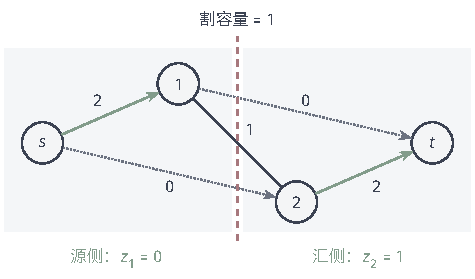
\includegraphics[width=80.405mm]{figures/06-probabilistic-graphical-models/02-inference/tikz/pgm-variational-cut/figure.pdf}
  \caption{两变量次模能量的$s$--$t$割网络。源侧编码为$0$，汇侧编码为$1$；实线终端边容量为$2$，点线终端边容量为$0$，中间无向边容量为$1$。虚线表示分开$\{s,1\}$和$\{2,t\}$的割，容量为$1$，对应配置$(0,1)$。}
  \label{fig:pgm-variational-cut}
\end{figure}

\subsubsection{多标签能量的局部优化}
\label{sec:pgm-variational-multilabel-cuts}

次模图割只解决二值问题。当每个变量有多个标签（不止0/1）时，一次割无法表达全部选择，常用的局部搜索是\emph{反复把多标签问题临时化成二元问题}：$\alpha$扩展每轮挑一个候选标签$\alpha$、让每个节点决定“保留现标签还是改成$\alpha$”（这一步在度量型代价下次模、可精确用图割解），逐轮尝试所有标签直到没有改进；$\alpha$-$\beta$交换则只允许当前标为$\alpha$或$\beta$的节点在这两个标签间重排。它们只保证局部最优，$\alpha$扩展在Potts能量下还有一个“至多两倍最优”的近似比保证。对多标签变量，一次$s$--$t$割只能表达两个选项。\term{$\alpha$扩展}（$\alpha$-expansion）固定当前标签$\ell_i$，让每个节点选择保留$\ell_i$或改为$\alpha$，把这一步化为二元问题。令动作变量$y_i=0$表示保留$\ell_i$、$y_i=1$表示改为$\alpha$，则一条边在四种动作下的代价为
\[
  \begin{array}{ccc}
      &y_j=0&y_j=1\\
    y_i=0&V_{i,j}(\ell_i,\ell_j)&V_{i,j}(\ell_i,\alpha)\\
    y_i=1&V_{i,j}(\alpha,\ell_j)&V_{i,j}(\alpha,\alpha)
  \end{array}.
\]
因此，能够使用上一小节的图割，取决于这张二元表是否次模。若成对项为$w_{i,j}d(k,l)$，$w_{i,j}\geq0$且$d$是标签上的度量，三角不等式给出
\[
  d(\ell_i,\ell_j)+d(\alpha,\alpha)
    \leq d(\ell_i,\alpha)+d(\alpha,\ell_j).
\]
所以每个扩展子问题次模，能精确求解。循环标签并只接受严格改善，有限状态下会停在对所有扩展动作都无法改进的配置，但未必是全局最优。

$\alpha$--$\beta$交换采用另一种二元动作：当前标为$\alpha$或$\beta$的节点是活跃节点，每个活跃节点独立选择$\alpha$或$\beta$，其他节点的标签保持固定。这不是强制两个节点互换标签；活跃节点可以共同改成同一标签。两个活跃节点之间的次模条件为
\[
  V_{i,j}(\alpha,\alpha)+V_{i,j}(\beta,\beta)
    \leq V_{i,j}(\alpha,\beta)+V_{i,j}(\beta,\alpha).
\]
例如，非负、对称且对角值为零的成对代价满足这一条件，即使它不满足标签间的三角不等式。只有一个端点活跃的边，在非活跃端标签固定后成为一元项，因此不会增加二元次模限制。交换由此可处理这类不能直接用于所有扩展动作的代价。

近似比保证还要固定原始能量的形式。对于
\[
  E(\bm\ell)=\sum_iD_i(\ell_i)
       +\sum_{(i,j)\in E}w_{i,j}\mathbb I[\ell_i\ne\ell_j],
  \qquad D_i(k)\geq0,\quad w_{i,j}\geq0,
\]
即非负一元项与非负边权的Potts能量，完全达到扩展局部最优的返回配置$\bm\ell_{\mathrm{return}}$满足经典保证$E(\bm\ell_{\mathrm{return}})\leq2E^\star$，其中$E^\star=\min_{\bm\ell}E(\bm\ell)$。这里要求对每个标签都已没有改善的扩展动作，提前停止并不能直接使用该保证。其他度量或不同停止状态需要相应的近似比分析；能量平移也会改变乘法比值，不能在任意移去常数后仍照用两倍界。更一般的扩展、交换与近似比结果参见Boykov等人\scite{pgm-variational-boykov2001}。

标签本身若有自然次序，还可能利用更强的代价结构。例如，标签为$0,\ldots,K-1$，成对代价为$w_{i,j}g(\ell_i-\ell_j)$、$w_{i,j}\geq0$，且$g$在允许的整数差值上满足$g(r+1)-2g(r)+g(r-1)\geq0$。这个二阶差分条件表示标签差每增加一单位所带来的增量代价不会下降，即离散凸性。在一元代价有限的这一设定下，可以把一个标签编码为一串有序阈值：标签为$k$，就表示它越过前$k$层阈值。多层图用这些阈值节点及保持次序的约束表示标签，在满足相应图表示条件时可一次精确求解。这条路线依赖有序标签和凸代价的结构，不能直接覆盖一般多标签能量\scite{pgm-variational-ishikawa2003}。

一般多标签或非次模能量仍可能需要其他松弛与搜索方法。二元变量的任意成对代价可写成常数、一次项和$z_iz_j$项之和；因为变量取布尔值而函数值取实数，这类目标称为二次伪布尔函数。某些相应松弛，例如具有持久性性质的图割松弛，可返回部分确定的$0/1$标签，其余节点标为未定。这里“确定”的保证是：至少存在一个全局最优配置，与所有已给出的标签相容；它不保证任意补全其余标签都最优。未定部分仍需继续求解、搜索或补全，并在原能量下评价最终配置\scite{pgm-variational-kolmogorov2007qpbo}。

\subsection{可行配置恢复与最优性诊断}

\label{sec:pgm-variational-tightness-rounding}

用松弛/对偶求得可计算上界，再通过取整或图割得到合法配置后，可用原始--对偶间隙评价该配置与最优值的距离。松弛值给出上界，已找到配置的真实得分给出下界；二者之差构成无需知道真值的次优性证书，间隙为零即证明全局最优。分数解在次模或树结构下可以无损取整，此时松弛是紧的。对于二元次模能量，共同阈值取整可以直接证明局部LP松弛是紧的。令$m_i=\mu_i(1)$。对任何局部一致的边表，$\Pr(Z_i\ne Z_j)\geq|m_i-m_j|$，因为$m_i-m_j=\mu_{i,j}(1,0)-\mu_{i,j}(0,1)$。非负$w_{i,j}$使松弛能量不小于
\[
  C+\sum_i[(1-m_i)D'_i(0)+m_iD'_i(1)]
       +\sum_{(i,j)}w_{i,j}|m_i-m_j|.
\]

令所有节点共用$U\sim\operatorname{Uniform}(0,1)$，取$z_i=\mathbb I[U<m_i]$，则节点均值为$m_i$，不同值概率恰为$|m_i-m_j|$。这个全局分布的期望能量等于上式，所以至少有一个阈值配置的能量不高于原LP解。用于LP最优解时，结合松弛下界便得到整数最优值等于LP最优值。因此LP存在整数最优解；存在平局时，若干整数最优解的分数混合也可能达到同一最优值。按排序后的$m_i$检查至多$d+1$个阈值区间即可寻找相应配置。

树图上的局部LP同样是紧的。局部一致表可以构造全局树分布，其期望得分不超过某个配置的得分，因此松弛最优值等于整数最优值，并存在整数最优解。树上的一般边缘仍可以是分数。含环图的紧性需要结合结构、势函数与参数判断，消息收敛本身只说明更新的状态。

对于一般LP分数解，可以逐点选择最大伪边缘、联合取整、局部搜索，或使用切平面和分支定界。逐点选择可能破坏变量之间的协调；存在硬约束时，还需检查恢复的配置是否可行，并在原目标下计算其得分。

对得分最大化，保留已找到的最好可行值$L=S(\widehat{\bm z})$及一个经验证的对偶上界$U$，则
\begin{equation}
  0\leq M-S(\widehat{\bm z})\leq U-S(\widehat{\bm z}).
  \label{eq:pgm-variational-gap}
\end{equation}
右侧是可计算的\term{原始--对偶间隙}（primal--dual gap），在此处比较整数可行解与松弛对偶证书。若还记录一个LP原始可行解$\bm\mu$的目标值$P=\langle\bm\theta,\bm\mu\rangle$，就能增加对求解过程的诊断，但要区分几个不同对象。对同一个LP及其对偶，有
\[
  U\geq U_{\mathrm{LP}}\geq M\geq L,
  \qquad P\leq U_{\mathrm{LP}}.
\]
其中$U$是对偶可行值，$U_{\mathrm{LP}}$是LP真正的最优值；$P$只是在当前分数可行点达到的值。由第一条链可知，$U-L$确实控制当前整数配置的次优损失。由第二条关系可知，$U-P\geq0$是可计算的LP求解差距，并且同时满足$0\leq U-U_{\mathrm{LP}}\leq U-P$与$0\leq U_{\mathrm{LP}}-P\leq U-P$。所以$U-P$小时，LP原始、对偶两侧的目标值都已接近LP最优值。

$P$与$L$之间却没有固定的大小关系。尚未充分优化的分数点可能比已经找到的合法配置得分还低，因此$P-L$不能无条件称为非负的“取整损失”。即使已经知道$P=U_{\mathrm{LP}}$，$P-L$也同时包含LP与整数问题的差别以及当前配置尚未最优的差别。更完整的关系为
\[
  U-L
    =(U-U_{\mathrm{LP}})
       +(U_{\mathrm{LP}}-M)+(M-L).
\]
三项依次是对偶尚未优化到LP最优值的差距、LP松弛间隙、当前配置相对整数最优值的次优损失，均非负。通常$U_{\mathrm{LP}}$和$M$并未知晓，后两项尤其不能仅凭当前$U,P,L$分别观测；记录三个当前值能提供证据，却不能自动完成这一分解。

对能量最小化，方向反过来：松弛或对偶提供下界，可行配置提供上界。在三角例中，逐点按平局选$0$得到得分$0$；把任一变量翻转便达到$2\beta$，但LP上界仍为$3\beta$。由于本例的整数真值与LP最优值都能独立算出，可以明确判断局部改进消除了当前配置的次优损失，却没有修复$\beta$的松弛间隙。再取三角例的均匀独立分布所诱导的局部表，得到LP原始可行值$P=3\beta/2$；与刚才的合法配置$L=2\beta$相比，$P-L=-\beta/2<0$，直接显示两者不具有固定顺序。

LP对偶的凸性支持全局求解，但求得$U_{\mathrm{LP}}$后，整数最优值仍可能更低。若一个合法配置达到对偶值，则配置与上界之间的间隙为零，可以立即形成全局最优证书。对于TRW消息算法，还需检查具体调度如何优化上界；目标的凸性与某种更新的单调性属于不同的论证。

MPE分解把计算分配给子问题。成对树上的一次最大和及回溯需$O(|E_T|k^2)$；多棵树可并行，但共享乘子的协调和通信仍在。显式局部LP有约$O(dk+mk^2)$个变量，其求解时间不只由变量数决定，还受求解器、约束和容差影响。图割属于多项式时间的特殊精确子问题，一次扩展只解一个二元动作，整体还要计入标签轮数。衡量可扩展性时，应同时报告单轮计算、存储、通信和达到所需诊断标准的轮数。

MPE近似需要另一套记录：原约束是否满足、可行配置得分是多少、对偶上界是多少，以及它们的差距。三角图的结论可同时列出：完全平均场的对数配分函数下界为$3.119162$，结构化固定点的同类下界为$3.178054$，精确$\log Z_\beta=3.258097$，Bethe固定点的对数配分函数近似为$3.295837$。MPE方面，最好可行得分为$2\log2=1.386294$，LP与该树分解的上界为$3\log2=2.079442$。前一组数值比较对数配分函数，后一组比较最大配置得分；它们需要分别展示对应的真值与界。

原始--对偶间隙直接控制当前配置相对于最优得分的损失。后验是否集中在该配置附近，以及各变量的边缘概率，还需由分布查询回答。间隙较大时，先用可计算的$U-P$检查LP是否还未求解充分，再尝试改进合法配置或加强一致性约束。对偶优化误差、松弛间隙和配置次优损失是不同来源；除非另有精确解或证书，不能声称已经把它们分别测出。可以根据现有上下界及改进结果，选择继续求解、加强松弛或接受已量化的总误差范围。配置推断的结果应同时包含合法配置及其得分证书。

\section{本章小结}

\label{sec:pgm-variational-summary}

本章以已知模型下的两类查询组织近似推断。对于后验分布，ELBO用反向KL连接近似分布与目标；平均场和结构化VI通过限制$q$的依赖，使期望和真实熵可计算。共轭消息、小批量更新与摊销映射分别减少局部期望计算、数据遍历和逐样本优化的成本，近似族误差则取决于所保留的结构。

局部自由能维护伪边缘，以局部一致性和熵近似替代全局分布计算。树上这些关系精确，推广到含环图后形成Bethe与Kikuchi近似；更大的区域保留更多联合约束，也增加表格和通信成本。EP以倾斜分布的矩修正站点，拉普拉斯法用峰附近曲率构造高斯。各方法的优化或固定点性质需要与实际概率查询的误差分别检查。

对于全部非证据变量的MPE，目标是最大配置得分。边缘多面体上的线性优化与这一查询等价，局部多面体松弛给出上界，对偶分解与TRW便于计算证书，二元次模等特殊结构可用图割直接返回整数最优解。配置结果通过可行性和原始--对偶间隙诊断，分布结果通过支持、相关性和预测诊断。含求和变量的边缘MAP还需保留其求和运算，另按对应查询求解。

\paragraph{扩展阅读}
Wainwright与Jordan系统联系了指数族、变分目标和图结构，可用于进一步理解边缘多面体与熵对偶。阅读时可围绕近似边缘、最优配置和配分函数分别比较目标、可行域及界的方向，并考察局部计算所保留的依赖\scite{pgm-wainwright2008}。

\chapter{基于采样的近似推断}
\label{chap:pgm-sampling}

第~\ref{chap:pgm-elimination}、\ref{chap:pgm-junction-tree}章的精确推断和第~\ref{chap:pgm-variational}章的变分近似，都用确定的数值或近似分布描述后验。采样推断不直接求出整个后验分布，而是从后验中抽取一批代表性随机样本：估计故障的后验概率时，统计样本中故障出现的比例；估计期望时，对样本上的函数值取平均。当中间因子过大、高维积分没有闭式解，或合适的变分分布族难以选定时，样本统计量通常较少依赖模型的具体解析形式。它的代价是答案带随机误差且通常只能近似；增加样本可以压低误差，同一批样本还能回答多个查询。

从后验采样通常并不比求后验更容易，因为实际往往只知道未归一化的联合权重$p(\bm{x},\bm{z})$，不知道归一化常数。本章讨论四种间接获得后验代表性样本的机制及其成立条件。直接从目标生成独立样本时，可用大数定律分析样本均值；目标难以直接采样时，重要性采样从提议分布生成候选，再用权重修正差异；高维下难以构造全局提议时，MCMC从当前状态作局部移动，靠满足条件的Markov链使长期访问比例逼近后验；观测随时间逐步到来时，序贯蒙特卡洛/粒子滤波递推样本与权重，并淘汰低质量样本。每种机制分别讨论估计量的极限条件、有限计算误差和诊断方法。

\section{采样推断的定义}
\label{sec:pgm-sampling-definition}

采样估计建立在一个共同事实上：如果存在一批独立且服从后验的样本，就可以用样本平均代替后验期望，并量化估计误差。后续各种采样器主要解决如何获得这样的样本。先设观测为$\bm{x}$，潜变量为$\bm{z}$，固定模型参数并省略其记号。把目标后验写为
\begin{equation}
  \begin{aligned}
    p(\bm{z}\mid\bm{x})&=\frac{\gamma(\bm{z})}{Z_{\bm{x}}},&
    \gamma(\bm{z})&=p(\bm{x},\bm{z}),\\
    Z_{\bm{x}}&=\int\gamma(\bm{z})\,\mathrm{d}\bm{z},&
    I_h&=\mathbb{E}_{p(\bm{z}\mid\bm{x})}[h(\bm{z})].
  \end{aligned}
  \label{eq:pgm-sampling-target}
\end{equation}
其中$0<Z_{\bm{x}}<\infty$，$h$是待求期望的实值函数。本章的积分也涵盖离散情形，此时改为求和，$p$表示概率质量而非密度。$\gamma$可以计算到一个与$\bm{z}$无关的正比例常数；这足以计算后验期望，却不足以确定原模型的证据$Z_{\bm{x}}$。估计证据时，必须知道$\gamma$的实际尺度。

若能直接从后验获得独立同分布的$\bm{z}_1,\ldots,\bm{z}_n$，就可以用函数值的样本均值估计$I_h$：
\begin{equation}
  \widehat I_{h,n}=\frac{1}{n}\sum_{i=1}^{n}h(\bm{z}_i).
  \label{eq:pgm-sampling-direct-estimator}
\end{equation}
选择$h(\bm{z})=\mathbb{I}\{\bm{z}\in B\}$，即事件$B$发生时取$1$、否则取$0$的指示函数，就得到后验事件概率的估计；选择某个分量或分量乘积，则得到均值或二阶矩。同一批样本可以用于多个查询，各查询的误差由相应的函数$h$决定。采样平均、方差缩减和Markov链长期平均的概率基础可参考\BookChapterRef{chap:random-sequences-and-processes}{卷2《数学准备：概率、因果与决策》的“随机序列与随机过程”章}。

独立样本的极限理论提供这一估计量的正确性依据。可积$h$使样本均值几乎必然收敛；方差$\sigma_h^2=\operatorname{Var}_p(h)$有限时，估计量还满足下列方差与极限关系：
\begin{equation}
  \begin{aligned}
    \mathbb{E}[\widehat I_{h,n}]&=I_h,&
    \operatorname{Var}(\widehat I_{h,n})&=\frac{\sigma_h^2}{n},\\
    \sqrt n(\widehat I_{h,n}-I_h)&\xrightarrow{\mathrm{d}}
      \mathcal{N}(0,\sigma_h^2).
  \end{aligned}
  \label{eq:pgm-sampling-iid-clt}
\end{equation}
\term{蒙特卡洛标准误}（Monte Carlo standard error, MCSE）衡量重复运行估计过程时答案的波动，即再独立抽取同样多的一批样本时平均答案的变动幅度。独立样本下可用$s_h/\sqrt n$估计，其中$s_h^2$是$h(\bm z_i)$的样本方差。它与后验标准差有明确区别：后者描述模型本身固有的不确定性（故障是否可能发生），不随样本增多而消失；MCSE描述有限采样带来的计算波动（对该概率估计的偏差程度），随$n$增大趋于零。


\begin{example}[报警后的故障概率]
  \label{ex:pgm-sampling-device}
  沿用人工构造的设备模型$F\to H\to A\leftarrow S$：$F$表示故障，$H$表示过热，$A$表示报警，$S$表示传感器失灵。根节点$F,S$独立，且
  \[
    \begin{aligned}
      p(F=1)&=0.1,&p(S=1)&=0.05,\\
      p(H=1\mid F=1)&=0.8,&
      p(H=1\mid F=0)&=0.1.
    \end{aligned}
  \]
  报警条件表仍与前面的精确推断相同：
  \[
    \begin{array}{ccccc}
      (h,s)&(0,0)&(1,0)&(0,1)&(1,1)\\
      p(A=1\mid h,s)&0.01&0.9&0.7&0.99
    \end{array}
  \]
  边缘化故障得到$p(H=1)=0.17$，从而
  \[
    \begin{aligned}
      p(A=1\mid H=0)&=0.95\times0.01+0.05\times0.7=0.0445,\\
      p(A=1\mid H=1)&=0.95\times0.9+0.05\times0.99=0.9045,\\
      p(A=1)&=0.83\times0.0445+0.17\times0.9045=0.1907,\\
      p(F=1,A=1)&=0.1(0.2\times0.0445+0.8\times0.9045)=0.07325.
    \end{aligned}
  \]
  因此精确答案为$p(F=1\mid A=1)=0.07325/0.1907\approx0.384111$。若能够取得$10000$个独立后验样本，故障比例的理论标准误约为$\sqrt{0.384111(1-0.384111)/10000}=0.004864$。这个小模型的精确答案用于校验采样计算，不是实际设备数据。
\end{example}

改变样本生成机制后，误差分析也要随之改变。重要性样本由提议生成，估计方差取决于加权函数；一条Markov链上的状态通常相关，样本均值的方差需要计入协方差；重采样粒子还可能共享祖先。后文分别建立这些机制下的正确性条件，再分析相应的计算误差。普通蒙特卡洛误差与方差缩减的系统论述见Owen\scite{pgm-sampling-owen2013}。

\section{独立蒙特卡洛方法}
\label{sec:pgm-sampling-independent}

这一节讲独立蒙特卡洛的三种递进办法：能直接按目标生成时直接采样；直接采样困难但能找到一个“罩住”目标的简单分布时，用拒绝采样筛选；连罩住都困难时，保留所有候选、改用连续权重修正，即重要性采样。三者每次都使用新的独立随机输入，候选彼此独立，但自归一化权重共用一个随机分母，估计量的分析还需考虑这一比值结构。

\subsection{直接采样、祖先采样与拒绝采样}
\label{sec:pgm-sampling-direct-rejection}

当目标分布本身带有容易操作的生成规则（例如有向图的局部条件分布）时，可以按变量之间的依赖顺序把一个完整样本“逐步抽出来”，无需知道难算的归一化常数。每次生成完整记录时使用新的独立随机输入，得到的记录之间才具有独立性。

在有向无环图上，\term{祖先采样}（ancestral sampling）按拓扑顺序逐个生成节点，使每个节点采样时都已知道其父节点的取值。若一次生成$\bm{x}$时，第$i$个节点使用$p(x_i\mid\bm{x}_{\operatorname{pa}(i)})$，则整次生成的概率恰为这些条件概率之积，也就是图模型的联合分布。样本内部的各节点通常不独立，独立的是从头运行得到的不同完整样本。一次生成的成本包括拓扑遍历和所有局部条件分布的采样成本；后者取决于各条件分布的实现。

祖先采样很容易抽到联合分布，但我们真正想要的是给定证据（如$A=1$）后的后验。一个朴素办法是：照常按先验抽完整样本，然后只保留恰好符合证据的样本、丢弃其余。在设备模型上，若按先验生成$F,S,H$后直接把$A$强行设为$1$，保留下来的故障比例仍是先验的$0.1$，并不是后验；只有连同$A$一起按模型生成、再仅保留$A=1$的样本，所保留记录才服从后验，故障概率为$0.384111$。这种“先从简单分布生成候选、再按某个规则决定去留”的做法就是\term{拒绝采样}（rejection sampling）的特例。

拒绝采样的一般设定是：找一个容易采样的提议分布$q$，并让它的密度在每一处都不低于目标密度（允许差一个常数倍），候选落在目标密度相对越高的位置就越可能被接受、越低则越可能被拒绝。设$q(\bm{z})$为提议密度，已知常数$c<\infty$使$\gamma(\bm{z})\leq c q(\bm{z})$在整个目标支撑集上成立。独立生成$\bm{z}\sim q$和$u\sim\operatorname{Uniform}(0,1)$，当$u\leq\gamma(\bm{z})/[c q(\bm{z})]$时接受。对任意可测集合$B$，
\begin{equation}
  \begin{aligned}
    \mathbb{P}(\bm{z}\in B,\text{接受})
      &=\int_B q(\bm{z})\frac{\gamma(\bm{z})}{c q(\bm{z})}
        \,\mathrm{d}\bm{z}
        =\frac{1}{c}\int_B\gamma(\bm{z})\,\mathrm{d}\bm{z},\\
    \mathbb{P}(\text{接受})&=\frac{Z_{\bm{x}}}{c}.
  \end{aligned}
  \label{eq:pgm-sampling-rejection}
\end{equation}
相除便得到$\mathbb{P}(\bm{z}\in B\mid\text{接受})=\int_B p(\bm{z}\mid\bm{x})\,\mathrm{d}\bm{z}$。因此按固定规则独立重复试验，直到得到指定数量的接受样本，会产生独立同分布的目标样本。每个接受样本平均需要$c/Z_{\bm{x}}$次提议。这一结论依赖全局包络条件。只检查已生成的位置，无法保证未访问区域也满足相同的接受规则。

在报警例子中，匹配证据的接受率为$0.1907$，平均约$5.244$次联合采样得到一个后验样本。若有多个稀有离散证据，联合匹配概率可能很小；连续证据的精确等值事件通常概率为零，需要使用密度条件化等其他采样构造。高维包络也容易变松：若归一化目标和提议分别按坐标分解，每维包络常数为$m>1$，乘积包络的接受率便是$m^{-d}$。后验越集中而提议越分散，越多计算会用在最终丢弃的候选上。

\subsection{重要性采样}
\label{sec:pgm-sampling-importance}

拒绝采样的最大问题是大量候选会被白白丢弃，尤其当证据稀有、维度很高时接受率极低。换个角度：与其把不太符合目标的候选直接扔掉，不如全都保留，但让每个候选对最终估计的“话语权”按它与目标的吻合程度加权——吻合得好的权重大、吻合得差的权重小。\term{重要性采样}（importance sampling, IS）正是这样做的：从易采样的$q$生成候选，并以目标与提议的密度比修正抽样频率。这要求$p\ll q$，即$q$必须覆盖目标的所有正概率区域（否则目标在那些区域的质量永远采不到、也无从修正）；连续情形按测度理解，零测集上的密度取值不影响结论。

如果目标密度已归一化，令$r(\bm{z})=p(\bm{z}\mid\bm{x})/q(\bm{z})$，便有
\begin{equation}
  \begin{aligned}
    I_h&=\int h(\bm{z})r(\bm{z})q(\bm{z})\,\mathrm{d}\bm{z},\\
    \widehat I_{h,n}^{\mathrm{IS}}
      &=\frac{1}{n}\sum_{i=1}^{n}r(\bm{z}_i)h(\bm{z}_i).
  \end{aligned}
  \label{eq:pgm-sampling-is}
\end{equation}
只要$\mathbb{E}_p|h|<\infty$，这个估计无偏且一致；有限方差还要求$\mathbb{E}_q[r^2h^2]<\infty$。目标区域若只被$q$赋予很小概率，偶尔出现的巨大权重会主导结果。支持覆盖保证目标区域有机会被提议访问，加权矩条件进一步控制罕见访问带来的波动。

图模型往往只提供$\gamma$。令$w_i=\gamma(\bm{z}_i)/q(\bm{z}_i)$，同时估计分子积分和归一化常数，得到\term{自归一化重要性采样}（self-normalized importance sampling, SNIS）：
\begin{equation}
  \begin{aligned}
    \widehat Z_{\bm{x}}&=\frac{1}{n}\sum_{i=1}^{n}w_i,&
    \bar w_i&=\frac{w_i}{\sum_{j=1}^{n}w_j},\\
    \widehat I_{h,n}^{\mathrm{SNIS}}
      &=\frac{\frac{1}{n}\sum_i w_i h(\bm{z}_i)}
              {\frac{1}{n}\sum_i w_i}
       =\sum_i\bar w_i h(\bm{z}_i).
  \end{aligned}
  \label{eq:pgm-sampling-snis}
\end{equation}
要求本次权重和非零。$\widehat Z_{\bm{x}}$无偏，但两个无偏估计的比值通常有偏，因为随机分母不能移到期望之外。在支撑集覆盖、$0<\mathbb{E}_q w=Z_{\bm{x}}<\infty$和$\mathbb{E}_q|wh|<\infty$时，分子、分母分别由大数定律收敛，故比值仍然一致。因此，比值的有限样本偏差与样本数增长后的渐近一致性可以同时成立。

设备例子可以令$q(f,h,s)=p(f)p(s)p(h\mid f)$，不抽取已知的$A$，而令$w(f,h,s)=p(A=1\mid h,s)$。这称为\term{似然加权}（likelihood weighting）：证据通过似然而非硬性筛选影响候选。图~\ref{fig:pgm-sampling-importance}比较先验与报警后的$(H,S)$分布。先验最常生成“既不过热也未失灵”，但这一状态很难解释报警；乘上似然以后，它只占约$4.13\%$的后验质量。

\begin{figure}[!t]
  \centering
  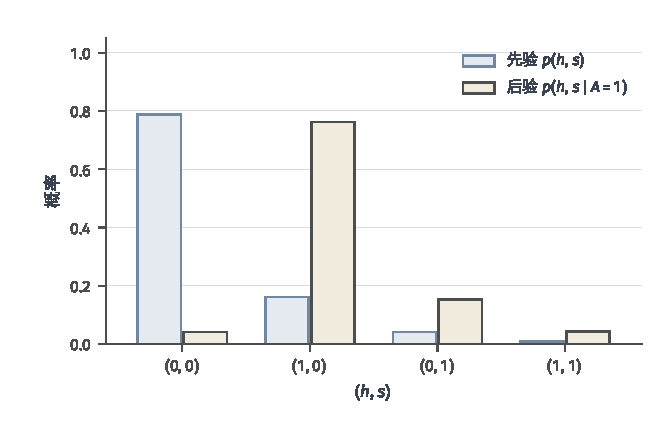
\includegraphics[width=105.412mm]{figures/06-probabilistic-graphical-models/02-inference/matplotlib/pgm-sampling-importance/figure.pdf}
  \caption{人工设备模型中$(H,S)$的先验与给定$A=1$后的后验。横轴每组的两位数依次为$h,s$；淡蓝柱表示先验，淡黄色柱表示后验。权重改变已有候选的贡献；未被抽到的类别仍需依靠后续生成访问。}
  \label{fig:pgm-sampling-importance}
\end{figure}

表~\ref{tab:pgm-sampling-weight-example}用四个可能的独立先验样本展示似然加权。直接计数的故障比例为$1/4$，加权比例为$0.9/(0.01+0.9+0.9+0.7)\approx0.358566$。权重按目标修正了候选贡献，但四次抽样仍有明显的有限样本波动，所得比例与精确后验不同。

\begin{table}[!t]
  \centering
  \begin{tabular}{ccccc}
    \toprule
    样本$i$ & $(f_i,h_i,s_i)$ & $w_i$ & $\mathbb{I}\{f_i=1\}$ & $w_i\mathbb{I}\{f_i=1\}$\\
    \midrule
    1 & $(0,0,0)$ & $0.01$ & $0$ & $0$\\
    2 & $(1,1,0)$ & $0.90$ & $1$ & $0.90$\\
    3 & $(0,1,0)$ & $0.90$ & $0$ & $0$\\
    4 & $(0,0,1)$ & $0.70$ & $0$ & $0$\\
    \bottomrule
  \end{tabular}
  \caption{似然加权的四样本教学计算。分母是全部权重之和，分子仅累加故障样本的权重。}
  \label{tab:pgm-sampling-weight-example}
\end{table}

提议的尾部决定极端权重出现的频率。即使提议很好地匹配后验峰附近，尾部事件估计仍需要足够的尾部覆盖。以一维标准正态目标$p=\mathcal{N}(0,1)$和$q=\mathcal{N}(0,s^2)$为例，其中$s>0$。二者的支撑集相同，但这只保证每个目标区域都有机会被访问。要判断权重的波动是否具有有限二阶矩，需要计算
\[
  \mathbb{E}_q[r^2]
    =\int \left(\frac{p(z)}{q(z)}\right)^2q(z)\,\mathrm{d}z
    =\int\frac{p(z)^2}{q(z)}\,\mathrm{d}z.
\]
将两个高斯密度代入，被积函数除去与$z$无关的正常数以后为
\[
  \frac{p(z)^2}{q(z)}
    \ \propto\ \exp\left[\left(-1+\frac{1}{2s^2}\right)z^2\right].
\]
当二次项系数$-1+1/(2s^2)$为负时，被积函数在两端都按高斯速度衰减，积分有限。系数为零时，被积函数是正常数，在整条实线上积分仍然发散；系数为正时，它随$|z|$增长，积分也发散。因此$\mathbb{E}_q r^2$只有在$s^2>1/2$时才有限。这是权重本身的二阶矩判据；具体查询的IS方差还要检查前述$\mathbb{E}_q[r^2h^2]$，不能仅凭权重二阶矩替任意$h$作保证。

提议过窄时，算法可以满足一致性的条件，却没有通常所需的有限权重二阶矩；重复运行中偶发的大权重会破坏熟悉的误差估计。如何构造尾部足够宽、同时不过度浪费样本的提议，是重要性采样的主要计算问题；相关分析可参见Owen教材的第9章\scite{pgm-sampling-owen2013}

\subsection{方差缩减}
\label{sec:pgm-sampling-variance-reduction}

增加样本数$n$总能压低误差，但代价是采更多样本。蒙特卡洛里还有另一类不增加样本、而是巧妙利用解析计算来减小单次随机贡献波动的办法，统称为方差缩减。这里介绍两种最常用的：一种用一个期望已知的相关量去抵消共同波动（控制变量），另一种把原本要靠抽样的部分改用精确积分算掉（Rao–Blackwell化）。

除了增加独立样本数，还可以通过减小单次随机贡献的方差来降低MCSE。设一次独立抽样原本给出随机贡献$Y$，待求量为$\mathbb{E}Y$。若能同时计算另一个随机量$G$，且其期望$\mu_G$已知，就可以用$G-\mu_G$记录这次抽样相对已知均值的偏离。对预先固定的系数$a$，以$Y-a(G-\mu_G)$替换$Y$不会改变期望，因为被减去部分的期望为零。这就是控制变量（control variates）的作用：利用已知期望修正样本函数。在$Y,G$均有有限方差时，
\[
  \operatorname{Var}\bigl(Y-a(G-\mu_G)\bigr)
    =\operatorname{Var}(Y)-2a\operatorname{Cov}(Y,G)
       +a^2\operatorname{Var}(G).
\]
若$\operatorname{Var}(G)>0$，使该二次式最小的系数为
\[
  a=\frac{\operatorname{Cov}(Y,G)}{\operatorname{Var}(G)}.
\]
代入这个系数后，方差的减少量为$\operatorname{Cov}(Y,G)^2/\operatorname{Var}(G)$。因此收益来自两种贡献之间可被抵消的共同波动，并非任意选择控制变量和系数都会减小方差。若总体协方差未知，可以用独立的先导样本估计$a$，再在正式抽样中固定该系数；若用同一批样本估计$a$并回代，系数与样本贡献会相互依赖，需另查偏差，不能直接继承固定系数时的无偏结论。

另一种波动来自完整记录中并非必须抽取的变量。若保留随机量$U$以后，仍能解析计算其余随机性下的条件平均，就可以把$Y$替换为$\widetilde Y=\mathbb{E}[Y\mid U]$。这种Rao--Blackwell化（Rao--Blackwellization）将部分抽样替换为条件积分。在图模型中，局部消元可以解析消去部分节点，仅对保留变量采样。条件积分必须使用原联合分布在给定$U$后的条件分布；这样的相容条件期望才保持原均值。由迭代期望和全方差关系，有限二阶矩下有
\[
  \begin{aligned}
    \mathbb{E}\widetilde Y&=\mathbb{E}Y,\\
    \operatorname{Var}(Y)
      &=\operatorname{Var}(\widetilde Y)
        +\mathbb{E}\bigl[\operatorname{Var}(Y\mid U)\bigr]
       \geq\operatorname{Var}(\widetilde Y).
  \end{aligned}
\]
被消去的是给定$U$以后仍会发生的抽样波动，右侧的条件方差项正好度量这部分波动。在相同独立抽样次数下，样本均值的方差也随之不增。

若目标是设备的先验报警概率，可以抽取完整$(F,H,S,A)$并平均$\mathbb{I}\{A=1\}$，也可以只抽取$F$，把其余节点解析消去。这里原贡献是$Y=\mathbb{I}\{A=1\}$，保留变量是$U=F$，所以替换后的贡献为$\mathbb{E}[Y\mid F]=p(A=1\mid F)$。它按原模型的$p(H,S,A\mid F)$积分，而非另换一个容易计算的条件分布。当$F=0$时，这个条件报警概率为$0.1305$；当$F=1$时为$0.7325$。两者均值都是$0.1907$，但前者单样本方差为$0.1907(1-0.1907)=0.15433351$，后者为$0.1\times0.9(0.7325-0.1305)^2=0.03261636$。解析计算减少了相同独立抽样次数下的方差；是否节约总时间，还要比较条件积分的成本。

方差缩减需要作用于完整估计量。SNIS的分子贡献为$wh$，分母贡献为$w$，因此要按提议的条件分布同时积分这两个量，保持权重与函数的相容关系。具体地，把提议下的变量分为$(U,V)$，仅抽取$U_i\sim q_U$，再计算
\[
  \begin{aligned}
    A(U)&=\mathbb{E}_q[w(U,V)h(U,V)\mid U],\\
    B(U)&=\mathbb{E}_q[w(U,V)\mid U],\\
    \widehat I_{h,n}^{\mathrm{RB\text{-}SNIS}}
      &=\frac{\sum_{i=1}^{n}A(U_i)}{\sum_{i=1}^{n}B(U_i)}.
  \end{aligned}
\]
这两个条件平均都使用$q(V\mid U)$，所以分子与分母的期望仍分别为$Z_{\bm{x}}I_h$和$Z_{\bm{x}}$。权重和非零且原来的可积性条件成立时，比值仍然一致；它通常仍有有限样本偏差。在对应二阶矩存在时，分子和分母各自的方差不增，仍不能单独推出其比值在每个有限样本量下也有更小方差，还须分析两者的共同波动。

为观察这一共同波动，可以在分析中把两者组合成$A(U)-I_hB(U)=\mathbb{E}_q[w(h-I_h)\mid U]$，实现上述估计时仍只需分别计算$A$和$B$。后文的比值展开会说明，$w(h-I_h)$正是原SNIS一阶误差的单样本贡献。因此在对应中心极限定理的矩条件下，对这个贡献取条件平均会使渐近方差不增；这个结论针对样本量增长时的一阶误差，不是所有有限样本比值的方差排序。MCMC均值的渐近方差还包括时间相关性，单次函数方差减小后，需要继续检查自相关如何变化。

\section{Markov链蒙特卡洛}
\label{sec:pgm-sampling-mcmc}

前面的独立方法（包括重要性采样）都隐含一个要求：能一次性构造一个在整个高维空间都覆盖良好的提议分布。但在高维、强相关的后验中，找到这样的全局提议往往和直接求后验一样难。换个思路：不必一次想清楚要跳到哪里，只要规定“站在当前位置时，下一步往附近怎么走”即可——用一个只依赖当前状态的局部规则反复走，走出一条状态序列；只要这个局部规则设计得当，长期来看序列造访各个状态的频率就会正比于其后验概率。\term{Markov链蒙特卡洛}（Markov chain Monte Carlo, MCMC）就是通过这样的局部转移形成\emph{相关}样本序列，再用长期平均近似目标期望。注意这些样本不再独立（相邻状态很接近），所以误差分析与独立样本不同；其正确性依赖两件事：转移规则保持目标分布，以及链长期运行能够充分访问目标的各个区域。

\subsection{Markov转移与目标分布}
\label{sec:pgm-sampling-markov-kernel}

局部转移规则必须保持目标分布不变。令$\bm z^{(k)}$为第$k$次迭代状态，$K(\bm z,B)$表示从当前状态转移到集合$B$的概率。若某一步的状态分布已经等于目标后验，再用该规则更新一步后仍应得到目标后验；否则这条链不能把目标分布作为稳定状态。把每个起点的后验权重与它转移到$B$的概率相乘并积分，就得到下一状态落入$B$的概率。要求它仍等于目标对$B$分配的概率，即
\begin{equation}
  \int p(\bm{z}\mid\bm{x})K(\bm{z},B)\,\mathrm{d}\bm{z}
    =\int_B p(\bm{z}'\mid\bm{x})\,\mathrm{d}\bm{z}'.
  \label{eq:pgm-sampling-invariance}
\end{equation}
满足此式时，$p$称为\term{平稳分布}（stationary distribution）：若当前状态已服从$p$，再转移一步仍服从$p$。该条件描述状态分布，单条轨迹仍可移动。但保持目标并不保证能从任意初值走到目标。例如，每一步都停在原地的规则保持任何分布，却只会反复输出同一个初值；它无法估计未访问区域的概率。从指定初值到达目标还需可达性等条件。

使往返概率流相等的细致平衡，是上述不变性的一个充分条件。在当前后验与转移核上，它写为
\begin{equation}
  p(\mathrm{d}\bm{z}\mid\bm{x})K(\bm{z},\mathrm{d}\bm{z}')
    =p(\mathrm{d}\bm{z}'\mid\bm{x})K(\bm{z}',\mathrm{d}\bm{z}).
  \label{eq:pgm-sampling-detailed-balance}
\end{equation}
测度记号包含拒绝后原地停留的点质量。对一端积分即可得到不变性。
顺次组合多个保持$p$的核仍保持$p$，但组合后的核未必可逆。

不变性之外，时间平均还需要链能够访问并返回目标的相关区域。对有限状态空间，不可约表示任意两个状态之间都能经有限步以正概率到达；这排除了被隔开的封闭状态类。有限不可约链的时间平均可收敛，但逐步状态分布收敛还需要非周期性，也就是返回时刻没有共同的、严格大于一的周期约束。例如，链确定地在$0$和$1$之间轮换，时间平均中两者的比例都趋于$1/2$；若从$0$启动，第$k$步的位置却由奇偶性决定，逐步状态分布不会趋于均匀分布。这个例子区分了长期访问比例与某一步位置的分布。

一般状态空间中，单点的目标概率可能为零，因而要把可达和返回的要求放在具有正目标概率的集合上。后文使用正Harris常返性：在所声明的状态类内，从每个起点出发，都以概率一反复访问每个具有正目标概率的可测集合，并且该类具有可归一化为概率分布的平稳测度。它把“能进入相关区域”加强为足以支持长期平均的返回性质。结合查询函数对目标分布可积，便可在这个状态类内讨论时间平均的几乎必然收敛；状态类之外的任意初值不自动包含在保证中。后文据此构造后验更新，再分别说明误差分析所用的起点条件，检查有限预算中的探索。

采样核的设计先检验不变性、可达性与返回条件，再分析探索速度。\term{混合}（mixing）描述链摆脱初值并访问目标分布的快慢。两个高概率区域之间存在低概率通道时，局部移动可能很难跨过它，即使渐近平均正确，有限预算中的估计仍可能偏向已访问的区域。

\subsection{Metropolis--Hastings方法}
\label{sec:pgm-sampling-mh}

现在给出最通用的MCMC规则Metropolis–Hastings（MH）：提议分布可以随便选，再用接受率校正它，使整条链保持目标分布，且不需要归一化常数。给定当前位置$\bm{z}$，设易采样提议为$q(\bm{z}'\mid\bm{z})$。若直接接受，往返概率流一般不相等。\term{Metropolis--Hastings方法}（Metropolis--Hastings, MH）通过位置相关的接受率，让实际往返流量都等于提议流量中较小的一方：
\begin{equation}
  \alpha(\bm{z},\bm{z}')
    =\min\left\{1,\,
      \frac{\gamma(\bm{z}')q(\bm{z}\mid\bm{z}')}
           {\gamma(\bm{z})q(\bm{z}'\mid\bm{z})}\right\}.
  \label{eq:pgm-sampling-mh-acceptance}
\end{equation}
从$\gamma(\bm{z})>0$的有效状态开始，提议到目标质量为零或无法反向提议的状态时拒绝；未实际提议到的零分母情形不参与该比值的计算。对两个不同状态，接受后的概率流为
\[
  \begin{aligned}
    &p(\bm{z}\mid\bm{x})q(\bm{z}'\mid\bm{z})\alpha(\bm{z},\bm{z}')\\
    &\qquad=\frac{\min\{\gamma(\bm{z})q(\bm{z}'\mid\bm{z}),
                    \gamma(\bm{z}')q(\bm{z}\mid\bm{z}')\}}
         {Z_{\bm{x}}}.
  \end{aligned}
\]
右侧交换$\bm{z},\bm{z}'$后不变；拒绝产生的原地停留也满足细致平衡。因此MH保持目标分布，并且不需要知道$Z_{\bm{x}}$。

MH每次先抽取提议，再用独立均匀数决定接受。接受时记录$\bm{z}'$，拒绝时继续记录$\bm{z}$。重复记录保留链在各状态停留的时间，删除这些记录会改变访问比例。独立拒绝采样以筛选得到目标独立样本，MH则以包含停留的相关轨迹保持目标。

随机游走提议常写作$\bm{z}'=\bm{z}+\epsilon\bm{\eta}$，其中$\bm{\eta}\sim\mathcal{N}(\bm{0},\bm{C})$，$\epsilon$为尺度，$\bm{C}$为给定正定矩阵。提议对称时，接受率只剩目标密度比。对标准正态目标，从$z=0$提议到$z'=2$的接受率是$\exp(-2)\approx0.1353$，反向提议则总被接受。尺度过小时，接受率虽高，每步位移却很小；尺度过大时，候选常落入低密度区域，链又因拒绝而停留。

维度会加重这一矛盾。对$p(\bm{z})\propto\exp(-\lVert\bm{z}\rVert_2^2/2)$，记$U(\bm{z})=-\log p(\bm{z})$并忽略其中与位置无关的常数。这个负对数密度也称势能：目标密度越小，势能越高。对称提议的接受率于是为$\min\{1,\exp[-\Delta U]\}$，其中$\Delta U=U(\bm{z}')-U(\bm{z})$。为看清维度的作用，这里固定每个坐标的噪声方差为$1$，取各向同性的$\bm{\eta}\sim\mathcal{N}(\bm 0,\bm I_d)$。势能变化为
\[
  \frac{\lVert\bm{z}+\epsilon\bm{\eta}\rVert_2^2
             -\lVert\bm{z}\rVert_2^2}{2}
    =\epsilon\bm{z}^{\top}\bm{\eta}
       +\frac{\epsilon^2}{2}\lVert\bm{\eta}\rVert_2^2.
\]
在这个固定噪声方差的设定下，$\mathbb{E}\lVert\bm{\eta}\rVert_2^2=d$，且其方差为$2d$，所以噪声平方范数通常与$d$同阶。若当前位置已服从标准高斯目标，且提议噪声独立，则交叉项$\epsilon\bm{z}^{\top}\bm{\eta}$的均值为零、方差为$\epsilon^2d$；正的二次项均值则为$\epsilon^2d/2$。固定$\epsilon>0$并增大$d$时，后者的增长快于交叉项的典型波动，使提议的势能差通常很大，接受率随之降低。将$\epsilon$缩小到与$d^{-1/2}$同阶可以控制这两个项的尺度，但每个坐标的提议位移也同时缩小，探索需要更多步。这些关系解释了固定尺度会让接受困难、缩小尺度又减缓单坐标探索的矛盾；它们针对当前高斯目标和固定坐标噪声方差的例子。一般后验的合适尺度还取决于其几何结构。

\term{独立提议}（independence proposal）取$q(\bm{z}'\mid\bm{z})=q(\bm{z}')$。候选不依赖当前位置，但接受后的链仍然相关。它能一次跨越很远的区域；为判断这种远距离候选能否被接受，把独立提议代入MH比值，得到
\[
  \frac{\gamma(\bm{z}')q(\bm{z})}
       {\gamma(\bm{z})q(\bm{z}')}
    =\frac{\gamma(\bm{z}')/q(\bm{z}')}
            {\gamma(\bm{z})/q(\bm{z})}
    =\frac{w(\bm{z}')}{w(\bm{z})},\qquad w=\frac{\gamma}{q}.
\]
因此接受率变成$\min\{1,w(\bm{z}')/w(\bm{z})\}$。一旦当前位置落入$q$严重低估的目标区域，当前权重$w(\bm{z})$就会很大；而从$q$生成的通常候选可能具有小得多的权重，使接受率很低。反复拒绝便使链在这一位置停留很久，尽管候选本身每次独立生成。独立提议依赖全局覆盖，随机游走依赖局部尺度。比较两者需要同时检查移动距离、停留和所需查询的估计误差。

\subsection{Gibbs采样}
\label{sec:pgm-sampling-gibbs}

MH需要自己设计提议和接受率。对图模型有一个更省事的特例：一次只更新一个变量，而该变量“在其余所有变量给定时的条件分布”往往因为Markov毯而形式简单、可以直接抽样——此时连接受率都是$1$，提议即被无条件接受。这就是Gibbs采样。图模型常允许直接计算一个变量在其余变量给定时的条件分布。\term{Gibbs采样}（Gibbs sampling）固定其余坐标，仅从待更新坐标的\term{满条件分布}（full conditional distribution）重新抽样；“满”表示已经给定其他全部未知变量及证据。记$\bm{z}_{-j}$为去掉第$j$个坐标后的向量，则单坐标更新使用$p(z_j\mid\bm{z}_{-j},\bm{x})$。顺序扫描时，一轮中已更新的坐标使用新值，尚未更新的坐标使用旧值。

满条件抽样可以看成接受率为一的MH更新。把固定$\bm{z}_{-j}$时的提议写成$q(z'_j\mid z_j,\bm{z}_{-j})=p(z'_j\mid\bm{z}_{-j},\bm{x})$，MH比值为
\begin{equation}
  \frac{p(z'_j,\bm{z}_{-j}\mid\bm{x})p(z_j\mid\bm{z}_{-j},\bm{x})}
       {p(z_j,\bm{z}_{-j}\mid\bm{x})p(z'_j\mid\bm{z}_{-j},\bm{x})}
    =1.
  \label{eq:pgm-sampling-gibbs-acceptance}
\end{equation}
等式来自联合分布的条件分解，并要求涉及的条件分布定义良好。每个更新核都保持后验，故依次组合一整轮也保持后验。若用近似满条件作提议，就不再有这个抵消；必须加入相应MH校正，或另行证明近似更新的偏差与收敛性质。随机扫描每次选一个坐标与确定性顺序扫描都可构造正确核，但整轮顺序扫描一般不满足细致平衡。

满条件虽然写成“给定所有其他变量”，实际计算通常只涉及邻近因子。有向图中，一个节点的\term{Markov毯}（Markov blanket）由父节点、子节点以及子节点的其他父节点组成；给定这些变量以后，其余节点不再改变该节点的条件分布。用$\operatorname{ch}(j)$记子节点集合，含有$z_j$的局部因子给出
\[
  p(z_j\mid\bm{z}_{-j},\bm{x})
    \ \propto\ p(z_j\mid\text{父节点})
       \prod_{\ell\in\operatorname{ch}(j)}
          p(v_\ell\mid\text{其父节点}),
\]
其中$v_\ell$表示子节点的当前取值，证据节点使用已观测值。无向图只需相乘所有包含该节点的势函数，再对候选$z_j$归一化。局部因子减少了单步计算范围，样本的跨迭代相关性仍取决于整个更新过程。

在设备后验$p(f,h,s\mid A=1)$上，更新$F$时只需$H$；若$H=1$，
\[
  p(F=1\mid H=1,A=1,S)
    =\frac{0.1\times0.8}{0.1\times0.8+0.9\times0.1}
    =\frac{8}{17}.
\]
更新$H$时则需$F,S,A$；若$F=1,S=0,A=1$，取$H=1$和$H=0$的未归一化概率分别为$0.8\times0.9=0.72$和$0.2\times0.01=0.002$，故前者的满条件概率是$0.72/0.722\approx0.997230$。更新$S$时，若$H=0,A=1$，则
\[
  p(S=1\mid H=0,A=1,F)
    =\frac{0.05\times0.7}{0.05\times0.7+0.95\times0.01}
    \approx0.786517.
\]
这三步展示了证据如何通过局部更新传播，而无须每次重新消去整张图。对有$K$个取值的节点，一次朴素更新需评估$K$组相关因子；块越大，联合条件分布的构造和抽样成本通常越高。

满条件更新的接受率为一，但强相关仍会限制每步移动。以零均值、相关系数$\rho\in(-1,1)$、边缘方差为$1$的二维高斯为例，其协方差矩阵为$\bigl(\begin{smallmatrix}1&\rho\\\rho&1\end{smallmatrix}\bigr)$。把联合密度中含$z_1$的二次项配方，有
\[
  z_1^2-2\rho z_1z_2+z_2^2
    =(z_1-\rho z_2)^2+(1-\rho^2)z_2^2.
\]
联合密度的指数是上述二次型乘以$-1/[2(1-\rho^2)]$。固定$z_2$后，配方后的第二项不影响$z_1$的条件密度，剩余部分正是均值$\rho z_2$、方差$1-\rho^2$的高斯密度，所以$z_1\mid z_2\sim\mathcal{N}(\rho z_2,1-\rho^2)$；交换两个坐标便得到$z_2\mid z_1$的相应表达式。满条件方差均为$1-\rho^2$，因此当$\rho$接近$1$时，给定一个坐标后另一个只能小幅移动。顺序更新满足
\[
  \begin{aligned}
    z_1^{(k+1)}&=\rho z_2^{(k)}+\sqrt{1-\rho^2}\epsilon_1,\\
    z_2^{(k+1)}&=\rho z_1^{(k+1)}+\sqrt{1-\rho^2}\epsilon_2,
  \end{aligned}
\]
其中每轮使用两个新的独立标准正态噪声$\epsilon_1,\epsilon_2$，它们也独立于此前的状态。把第一式代入第二式，得到
\[
  z_2^{(k+1)}
    =\rho^2z_2^{(k)}
      +\sqrt{1-\rho^2}(\rho\epsilon_1+\epsilon_2).
\]
新噪声独立于$z_2^{(k)}$，方差为$(1-\rho^2)(1+\rho^2)=1-\rho^4$，所以$z_2$跨一轮的自回归系数为$\rho^2$。若链已处于目标平稳分布，$\operatorname{Var}(z_2^{(k)})=\operatorname{Var}(z_2^{(k+1)})=1$，相邻两轮的协方差就是$\rho^2$，相邻相关系数也为$\rho^2$。因此即使每次都接受，$\rho=0.99$时平稳轨迹仍有$0.9801$的一步相关。非平稳启动时递推中的系数仍为$\rho^2$，但不能在尚未具有平稳方差时直接把它称为实际相邻相关系数。

要减少这种逐坐标移动的限制，可以把强相关坐标合为一块。\term{分块Gibbs采样}（blocked Gibbs sampling）从这一块在其余坐标给定时的联合条件分布抽样，使多个坐标在一次更新中沿联合条件的相关方向共同移动。在上述二维高斯例子中，若将两个坐标组成完整的块，就可以直接从二维联合高斯重新抽取；这避免了必须轮流等待另一个坐标改变的限制。对更大的图，构造和抽取块条件分布也会增加单步成本。

若部分变量可以解析积分，还可以先减少需要在链上更新的对象。\term{折叠Gibbs采样}（collapsed Gibbs sampling）将潜变量分为$(U,V)$，先解析消去$V$，得到边缘目标$p(U\mid\bm{x})=\int p(U,V\mid\bm{x})\,\mathrm{d}V$，再对$U$的各坐标构造这一边缘目标下的满条件。完整样本可在取得$U$以后，从$p(V\mid U,\bm{x})$补抽；当$U$服从边缘目标时，边缘分布与这个条件分布相乘恰好重建原联合后验。折叠减少采样维度，也可能形成稠密因子并提高单步成本。所有保留坐标的更新都应与折叠后的同一边缘目标相容，不能任意混用消元前后的条件分布。

确定性约束还可能使单坐标链完全无法离开当前配置。例如，两个二值变量的合法状态只有$(0,0)$和$(1,1)$，且两者目标概率均为正。处于$(0,0)$时，固定任一坐标为$0$，另一个坐标的满条件也只能取$0$，所以两个单坐标更新都不会移动；从$(1,1)$启动同样会停住。把两个坐标联合更新，则可以按目标概率在这两个合法状态之间切换。此时需要改变分块或参数化以恢复可达性，接受率为一也不能替代这一要求。Koller与Friedman的第12章讨论了这些构造及其限制\scite{pgm-koller2009}。

\subsection{Hamiltonian Monte Carlo}
\label{sec:pgm-sampling-hmc}

逐坐标的Gibbs在变量高度相关时会“走不动”：每步只能沿一个坐标轴小幅移动。对连续、可微且变量强相关的后验，Hamiltonian Monte Carlo（HMC）借鉴物理思想，引入一个“动量”让状态像粒子一样沿势能坡滑行，从而一次提议就能朝相关方向移动较远。\term{哈密顿蒙特卡洛}（Hamiltonian Monte Carlo, HMC）引入辅助动量，让当前位置沿由梯度决定的轨迹移动，再把轨迹末端作为一次整体提议。梯度在这里决定扩展状态的动力学轨迹，后文将说明这一轨迹如何构成保持目标的采样更新。

以下讨论$\mathbb{R}^{d}$上$\gamma>0$且足够光滑的情形，使用固定的对称正定\term{质量矩阵}（mass matrix）$\bm{M}\in\mathbb{R}^{d\times d}$控制不同方向的运动尺度。令辅助动量$\bm{r}\in\mathbb{R}^{d}$服从$\mathcal{N}(\bm{0},\bm{M})$。该正态密度的负对数除去常数后为$\frac12\bm{r}^{\top}\bm{M}^{-1}\bm{r}$；我们把这一项作为动能，与负对数目标给出的势能$U(\bm{z})=-\log\gamma(\bm{z})$相加。这样定义总能量，就能把原位置密度和辅助动量密度写成同一个指数形式：
\begin{equation}
  \begin{aligned}
    H(\bm{z},\bm{r})&=U(\bm{z})+\frac12\bm{r}^{\top}\bm{M}^{-1}\bm{r},\\
    \widetilde p(\bm{z},\bm{r})
      &=p(\bm{z}\mid\bm{x})\mathcal{N}(\bm{r};\bm{0},\bm{M})
        \ \propto\ \exp[-H(\bm{z},\bm{r})].
  \end{aligned}
  \label{eq:pgm-sampling-hamiltonian}
\end{equation}
把动量积分掉，仍得到原目标后验。动量只是计算辅助变量；其分布与$\bm{z}$独立，因而每轮在保持$\bm{z}$不变时重新抽取$\bm{r}$，就是扩展分布上的一次精确条件更新。这一\term{动量刷新}（momentum refreshment）保持$\widetilde p$，并使相邻轨迹能具有不同能量和方向。若只做确定性能量守恒运动而不刷新，轨迹会局限在某个能量面，通常无法遍历扩展分布。

有了扩展密度，我们还需要选择如何沿轨迹移动。用$s$表示轨迹内部的人工连续时间，避免与观测时间混淆。动能对动量的梯度为$\nabla_{\bm r}H=\bm M^{-1}\bm r$，可以用作位置的运动速度；势能梯度$\nabla U$指向负对数目标增大的方向，动量沿相反方向改变。把这两个变化配成Hamilton方程，便得到
\begin{equation}
  \frac{\mathrm{d}\bm{z}}{\mathrm{d}s}=\bm{M}^{-1}\bm{r},
  \qquad
  \frac{\mathrm{d}\bm{r}}{\mathrm{d}s}=-\nabla U(\bm{z}).
  \label{eq:pgm-sampling-hamilton-equations}
\end{equation}
这一对变化的符号使能量交换恰好抵消。沿轨迹对$H$求导，可得
\[
  \frac{\mathrm dH}{\mathrm ds}
  =\nabla U(\bm z)^{\top}\bm M^{-1}\bm r
   +(\bm M^{-1}\bm r)^{\top}[-\nabla U(\bm z)]
  =0.
\]
位置移动导致的势能变化，恰好由动量变化导致的动能变化补偿，因此精确轨迹守恒总能量。方程还有另一项作用：位置速度$\bm M^{-1}\bm r$不依赖位置，动量速度$-\nabla U(\bm z)$不依赖动量，所以扩展空间速度场的散度为
\[
  \nabla_{\bm z}\!\cdot(\bm M^{-1}\bm r)
  +\nabla_{\bm r}\!\cdot[-\nabla U(\bm z)]=0.
\]
散度描述一个微小体积在流动中的相对变化率；这里为零，说明流不会压缩或膨胀扩展状态的小体积。在流存在且光滑的区间内，这就给出体积保持。能量守恒使$\exp(-H)$的密度值沿轨迹不变，体积保持使同一小块所承载的概率质量也不变，两项性质共同保证精确流保持$\widetilde p$。相关动力系统背景可参考\BookChapterRef{chap:dynamical-systems-and-state-estimation}{卷2《数学准备：概率、因果与决策》的“动力系统”章}。

实际计算通常不能直接求出精确流，需要用离散轨迹近似。先固定位置，动量便按当前的恒定力$-\nabla U(\bm z)$变化；再固定动量，位置便按速度$\bm M^{-1}\bm r$匀速变化。这两种简单更新都能直接计算。\term{蛙跳积分}（leapfrog integration）把动量半步、位置整步和动量半步对称排列，以组合近似原来的同时运动。令$\epsilon>0$为一步的人工时间长度，对后验势能$U$的一步更新为
\begin{equation}
  \begin{aligned}
    \bm{r}_{1/2}&=\bm{r}-\frac{\epsilon}{2}\nabla U(\bm{z}),\\
    \bm{z}'&=\bm{z}+\epsilon\bm{M}^{-1}\bm{r}_{1/2},\\
    \bm{r}'&=\bm{r}_{1/2}-\frac{\epsilon}{2}\nabla U(\bm{z}').
  \end{aligned}
  \label{eq:pgm-sampling-leapfrog}
\end{equation}
下标$1/2$只是一步内部的半步标记，两个动量半步各用时$\epsilon/2$，中间位置步用时$\epsilon$。蛙跳通常有能量误差，但在精确算术下保留体积和可逆性，便于下一步作概率校正。固定正整数$L$作为步数，重复上述更新后就得到人工时间长度$\tau=L\epsilon$的离散轨迹。

保体积可以逐步验证。动量更新的Jacobian是对角块均为单位矩阵的下三角块矩阵，位置更新则是相应的上三角块矩阵；二者行列式均为$1$。三步复合以及重复$L$步后的映射$\Phi_{\epsilon}^{L}$仍保体积。可逆性来自对称的半步排列：把末端动量变号，按相同步长和步数再运行，再次变号，就回到起点。令$R(\bm{z},\bm{r})=(\bm{z},-\bm{r})$，则
\begin{equation}
  R\Phi_{\epsilon}^{L}R=(\Phi_{\epsilon}^{L})^{-1},
  \qquad
  T=R\Phi_{\epsilon}^{L},\qquad T^2=\operatorname{id}.
  \label{eq:pgm-sampling-hmc-reversibility}
\end{equation}
因此“积分后翻转动量”的提议$T$是一个自身为逆的保体积映射。翻转不改变动能，其作用是让提议明确具有可对应的反向路径。

设$\bm{y}=(\bm{z},\bm{r})$、$\bm{y}'=T\bm{y}$，末端\term{Metropolis校正}（Metropolis correction）的接受率为
\begin{equation}
  \alpha_H(\bm{y},\bm{y}')
    =\min\{1,\exp[-H(\bm{y}')+H(\bm{y})]\}.
  \label{eq:pgm-sampling-hmc-acceptance}
\end{equation}
这一接受率利用了$T$的两项性质：自身为逆使正反提议配对，保体积使Jacobian修正为$1$。两方向的接受流量都正比于
\[
  \min\bigl\{\exp[-H(\bm{y})],\exp[-H(\bm{y}')]\bigr\},
\]
因而满足扩展空间的细致平衡。刷新动量与该接受／拒绝更新各自保持$\widetilde p$，两者复合也保持它；只保留位置就得到保持原后验的转移核。因此，可逆性建立反向路径，体积保持控制坐标变换，末端接受率修正能量误差，三者共同形成保持目标的更新\scite{pgm-sampling-neal2011}。

\Needspace{22\baselineskip}
\begin{algorithm}[固定步长与轨迹长度的HMC]
  \label{alg:pgm-sampling-hmc}
  \begin{algorithmic}[1]
    \Require 有效初始位置$\bm{z}^{(0)}$，可计算的$U,\nabla U$
    \Require 固定对称正定$\bm{M}$、$\epsilon>0$、正整数$L,n$
    \Ensure 含拒绝后重复位置的$n$个MCMC样本
    \For{$k=0,\ldots,n-1$}
      \State 抽取$\bm{r}\sim\mathcal{N}(\bm{0},\bm{M})$，记$\bm{y}=(\bm{z}^{(k)},\bm{r})$
      \State 从$\bm{y}$按式~\eqref{eq:pgm-sampling-leapfrog}积分$L$步
      \State 翻转末端动量，得到$\bm{y}'=(\bm{z}',-\bm{r}')$
      \State 抽取$u\sim\operatorname{Uniform}(0,1)$
      \If{$u\leq\alpha_H(\bm{y},\bm{y}')$}
        \State $\bm{z}^{(k+1)}\gets\bm{z}'$
      \Else
        \State $\bm{z}^{(k+1)}\gets\bm{z}^{(k)}$
      \EndIf
      \State 记录$\bm{z}^{(k+1)}$；本轮动量随后丢弃
    \EndFor
  \end{algorithmic}
\end{algorithm}

算法中的有效初始位置要求目标密度为正，且势能和梯度可计算；上述$\mathbb R^d$上的正光滑目标设定正是为此服务。算法描述理想算术下的更新，数值实现还须检测积分和能量是否有限；积分失败时应拒绝本轮提议、保留原位置，并记录失败，不能把未定义的能量送入接受率计算。

对$p(z)=\mathcal{N}(0,1)$、$M=1$，有$U(z)=z^2/2$。从$(z,r)=(0,1)$以$\epsilon=0.5$走一步，得到$r_{1/2}=1$、$z'=0.5$和$r'=0.875$。这里$r'$是蛙跳积分末端、尚未翻转的动量；提议映射$T$再把它变为$-0.875$，位置仍为$0.5$。翻转不改变动能，故起点能量为$0.5$，末端为$(0.5^2+0.875^2)/2=0.5078125$，接受率为$\exp(-0.0078125)\approx0.992218$。图~\ref{fig:pgm-sampling-hmc}把这个离散步与精确能量圆并列，展示离散化造成的能量偏移。Metropolis步骤按这一偏移校正接受率；有限链长与慢混合仍需通过运行和诊断处理。

\begin{figure*}[!t]
  \centering
  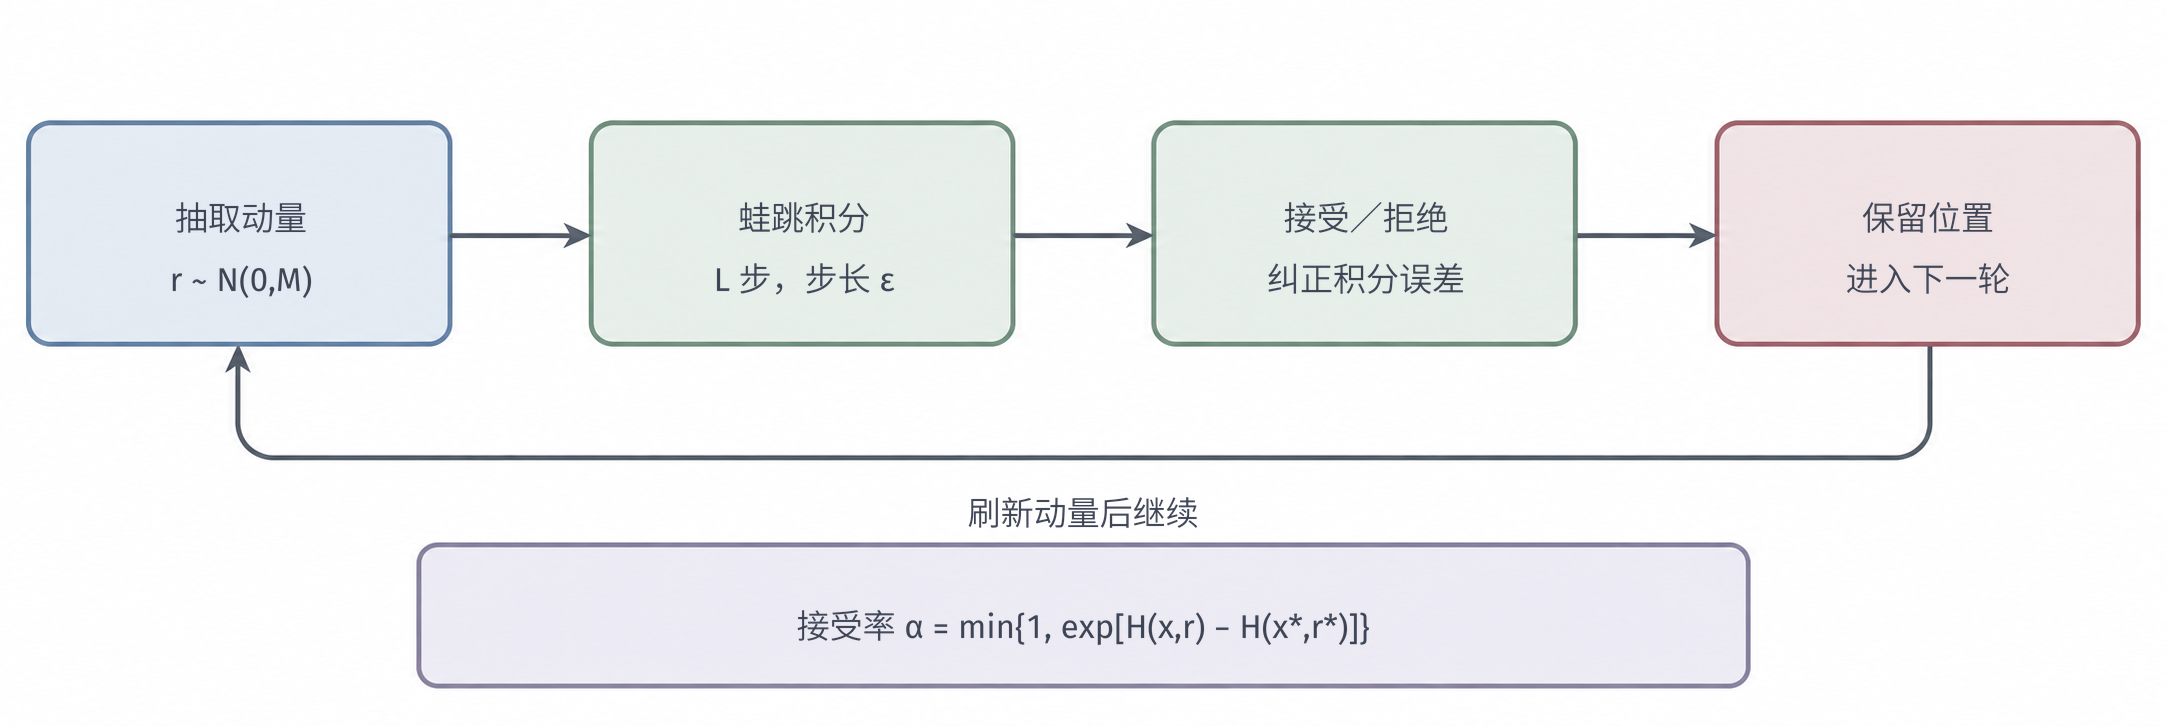
\includegraphics[width=169.000mm]{figures/06-probabilistic-graphical-models/02-inference/generated/pgm-sampling-hmc/figure.png}
  \par\medskip
  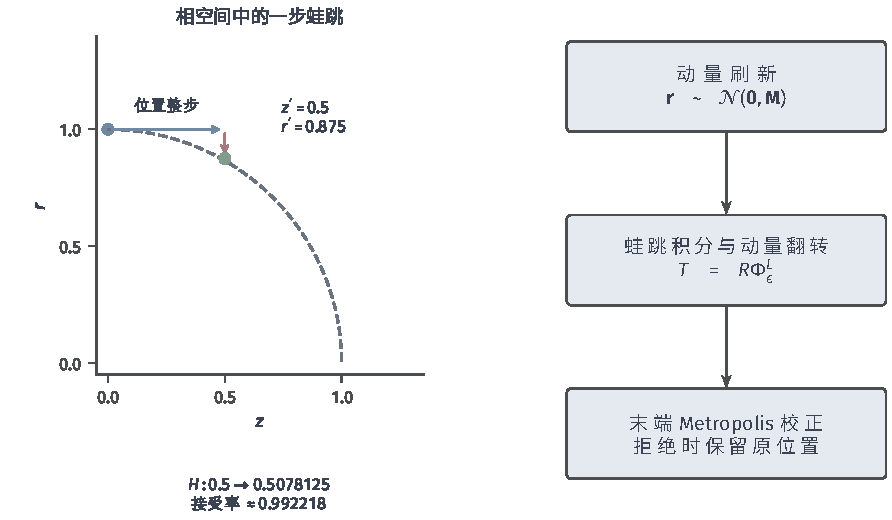
\includegraphics[width=142.118mm]{figures/06-probabilistic-graphical-models/02-inference/matplotlib/pgm-sampling-hmc/figure.pdf}
  \caption{HMC的更新流程与标准正态目标的一步数值计算。上方依次刷新动量、执行蛙跳并翻转末端动量、接受或拒绝提议、记录位置；$\bm z$是位置，$H$表示扩展状态的哈密顿量。下方的数值图由解析式生成：虚线圆弧属于$H=1/2$的精确轨迹，折线表示$\epsilon=0.5$的蛙跳整步与末端动量半步；初始动量半步因$z=0$不移动。动量翻转未画在相图上，接受率约为0.992218。}
  \label{fig:pgm-sampling-hmc}
\end{figure*}

步长$\epsilon$决定局部积分精度，轨迹长度$\tau=L\epsilon$决定一次提议运动多久。在足够光滑、数值稳定且$\tau$固定的条件下，蛙跳的全局状态误差为$O(\epsilon^2)$；在相应有界区域内，能量误差也可控制在这一阶。误差常数依赖曲率、维度和轨迹，采样误差还取决于链的探索。过大步长可能造成能量误差突然增大、非有限数值或拒绝；此类积分失败应拒绝并记录。过短轨迹探索不足，过长轨迹可能绕回原处，增加梯度计算却没有相应收益。

质量矩阵改变的是运动几何。为了看清它与目标尺度的关系，考虑高斯目标$\mathcal{N}(\bm{0},\bm{\Sigma})$，其中$\bm\Sigma$对称正定。此时$U(\bm z)=\tfrac12\bm z^{\top}\bm\Sigma^{-1}\bm z$加上常数，故$\nabla U(\bm z)=\bm\Sigma^{-1}\bm z$。由于$\bm M$固定，对位置方程再求一次导数，并代入动量方程，就得到
\[
  \frac{\mathrm{d}^2\bm{z}}{\mathrm{d}s^2}
     =\bm M^{-1}\frac{\mathrm d\bm r}{\mathrm ds}
     =-\bm{M}^{-1}\bm{\Sigma}^{-1}\bm{z}.
\]
按本章动量协方差等于$\bm M$的约定，取$\bm M=\bm\Sigma^{-1}$后，右侧变为$-\bm z$。每个坐标都满足$\mathrm d^2z_j/\mathrm ds^2=-z_j$，即频率为$1$的简谐运动；原来不同方向的快慢因而在人工时间下得到统一。软件中的“度量”和“逆质量”可能采用相反矩阵约定，使用时应先核对动量协方差与动能公式。固定矩阵补偿的是全局线性尺度；随位置变化的狭窄区域和多峰障碍需要其他几何或采样处理。通常在预热阶段调整尺度，正式保留样本时固定参数；任意依赖历史的持续调整不能直接套用上述齐次链证明。

若一次梯度求值成本为$C_{\nabla U}$，一轮HMC约需$O(L C_{\nabla U})$，另加动量生成和质量矩阵运算。对角矩阵的线性代数成本为$O(d)$每步，稠密矩阵通常为$O(d^2)$每步，并需预先分解。标准HMC不能直接更新离散变量；受约束连续变量常需先变换到无约束空间，并把变换的Jacobian加入密度。

计算出一条长轨迹也不保证位置移动有效。以标准正态和$M=1$的精确流为例，位置满足$z(s)=z(0)\cos s+r(0)\sin s$。若固定轨迹长度为$2\pi$，则不论本轮刷新出什么动量，末端位置都回到$z(0)$；精确积分的接受率虽为$1$，位置链却不移动。这就是固定长度与运动周期\term{共振}（resonance）妨碍遍历的一个最小例子。因此，积分误差控制之外仍需另外检查链的探索能力。

\section{序贯蒙特卡洛}
\label{sec:pgm-sampling-smc}

前面的MCMC针对“一个固定的后验分布”反复采样。但在很多实际问题里，观测是随时间一个接一个到来的（传感器持续上报、目标不断移动），目标分布每个时刻都在变；若每来一个观测就从头跑一条MCMC链，代价太高。自然的想法是让一群带权样本（粒子）随时间一起“向前走”，并在新观测到来时调整它们的权重。\term{序贯蒙特卡洛}（sequential Monte Carlo, SMC）复用上一阶段的样本及权重，逐步追踪一列目标分布。带权样本称为\term{粒子}（particle），每个粒子表示一个可能的潜在状态或状态历史。

为建立最小动态设定，令潜在状态为$\bm{z}_t$、观测为$\bm{x}_t$，真实时间$t=1,\ldots,T$写作下标。初始分布为$p(\bm{z}_1)$，转移分布为$p(\bm{z}_t\mid\bm{z}_{t-1})$，观测分布为$p(\bm{x}_t\mid\bm{z}_t)$。其联合分布分解为
\begin{equation}
  \begin{aligned}
    &p(\bm{z}_{1:T},\bm{x}_{1:T})\\
    &\qquad=p(\bm{z}_1)p(\bm{x}_1\mid\bm{z}_1)
       \prod_{t=2}^{T}
         p(\bm{z}_t\mid\bm{z}_{t-1})p(\bm{x}_t\mid\bm{z}_t).
  \end{aligned}
  \label{eq:pgm-sampling-state-space}
\end{equation}
这里假设给定上一潜状态后，更早状态不再影响当前状态；给定当前潜状态后，当前观测不再依赖其余变量。\term{滤波}（filtering）的目标是$p(\bm{z}_t\mid\bm{x}_{1:t})$，只利用截至当前的观测估计当前状态。若利用未来观测估计过去状态，则是平滑问题。本节只建立粒子计算所需的模型；第~\ref{sec:pgm-dynamic-common}节将从动态有向分解系统建立这些查询，第~\ref{sec:pgm-dynamic-continuous}节再比较何时可以用解析滤波代替粒子近似。

SMC不只适用于物理时间。一列$\gamma_\ell(\bm{z})=p(\bm{z})p(\bm{x}\mid\bm{z})^{\beta_\ell}$，其中$0=\beta_0<\cdots<\beta_L=1$，也可让粒子逐步从先验迁移到后验。这里的$\beta_\ell$是似然的指数，通常称为逆温度参数；指数从$0$增至$1$，表示逐步增强同一组观测对目标的影响，而不是增加新的观测。设各阶段归一化常数有限且为正，先验阶段按$\gamma_0=p(\bm z)$定义。对已有粒子，相邻阶段在其取值处的目标比为
\[
  \frac{\gamma_\ell(\bm z)}{\gamma_{\ell-1}(\bm z)}
    =p(\bm x\mid\bm z)^{\beta_\ell-\beta_{\ell-1}},
\]
其中比值只在前一阶段目标为正的位置计算；零似然位置在正指数阶段得到零权重。粒子据此更新权重，再按需要重采样，并进行保持当前归一化目标的MCMC移动。权重负责相邻目标的改变，MCMC核则在目标固定的当前阶段移动粒子。这里的$\ell$标记逆温度递增的算法阶段，与观测时间不同。本节以\term{粒子滤波}（particle filtering）为主，即用SMC近似式~\eqref{eq:pgm-sampling-state-space}的滤波分布。

\subsection{序贯重要性采样}
\label{sec:pgm-sampling-sis}

序贯重要性采样（SIS）就是把重要性采样改造成可随时间递推的形式：旧粒子继续保留，每步只需让它按状态转移“向前走一步”，再用新观测更新权重，而不必重算整条路径。路径后验涉及截至当前的全部潜状态，路径中的潜状态数量随时间增长。利用Markov分解，可以保留旧路径，只生成当前状态并更新权重。\term{序贯重要性采样}（sequential importance sampling, SIS）把路径提议写成
\[
  q_{1:t}(\bm{z}_{1:t}\mid\bm{x}_{1:t})
    =q_1(\bm{z}_1\mid\bm{x}_1)
      \prod_{s=2}^{t}
        q_s(\bm{z}_s\mid\bm{z}_{1:s-1},\bm{x}_{1:s}),
\]
其中每个$q_s$保持该阶段生成路径时所用的规则，使旧路径的提议密度仍由同一公共前缀表示。选择未归一化路径目标$\gamma_t=p(\bm{z}_{1:t},\bm{x}_{1:t})$。对$t\geq2$，新目标与新提议分别等于旧前缀乘上一个当前因子：
\[
  \begin{aligned}
    \gamma_t(\bm z_{1:t})
      &=\gamma_{t-1}(\bm z_{1:t-1})
          p(\bm z_t\mid\bm z_{t-1})p(\bm x_t\mid\bm z_t),\\
    q_{1:t}(\bm z_{1:t}\mid\bm x_{1:t})
      &=q_{1:t-1}(\bm z_{1:t-1}\mid\bm x_{1:t-1})
          q_t(\bm z_t\mid\bm z_{1:t-1},\bm x_{1:t}).
  \end{aligned}
\]
把两行相除，旧目标与旧提议的比值正是上一时刻的路径权重。因而不必重新计算整条路径的所有因子，只需保留旧权重，再乘新增目标因子与新增提议因子的比值。逐粒子写出这一关系，得到
\begin{equation}
  \begin{aligned}
    w_{1,i}&=
      \frac{p(\bm{z}_{1,i})p(\bm{x}_1\mid\bm{z}_{1,i})}
           {q_1(\bm{z}_{1,i}\mid\bm{x}_1)},\\
    w_{t,i}&=w_{t-1,i}
      \frac{p(\bm{z}_{t,i}\mid\bm{z}_{t-1,i})
            p(\bm{x}_t\mid\bm{z}_{t,i})}
           {q_t(\bm{z}_{t,i}\mid\bm{z}_{1:t-1,i},\bm{x}_{1:t})}.
  \end{aligned}
  \label{eq:pgm-sampling-sis-weight}
\end{equation}
下标$i=1,\ldots,n$标记粒子，$\bm{z}_{1:t,i}$是第$i$条路径。提议必须覆盖其对应的目标条件支撑集。权重的绝对尺度对归一化均值无影响，因此递推时可用上一时刻的归一化权重，再统一归一化当前权重。

路径后验中关于当前状态的查询，只使用$h(\bm z_t)$，与同一路径上更早坐标的具体记法无关。把路径经验分布对旧坐标边缘化，就相当于保留每条路径的权重和末端位置；这个操作不会把原来的不同权重自动变为等权。只保留路径末端，就得到滤波分布的经验近似
\begin{equation}
  \begin{aligned}
    \widehat p_t(\mathrm{d}\bm{z})
      &=\sum_{i=1}^{n}\bar w_{t,i}\delta_{\bm{z}_{t,i}}(\mathrm{d}\bm{z}),\\
    \widehat I_{t,h}&=\sum_{i=1}^{n}\bar w_{t,i}h(\bm{z}_{t,i}).
  \end{aligned}
  \label{eq:pgm-sampling-particle-measure}
\end{equation}
其中$\delta_{\bm{z}_{t,i}}$是把全部概率质量放在该粒子位置的点质量分布，不是连续密度曲线。若连续目标没有点质量，则有限粒子近似与它不可能在总变差距离下趋近。为看清这一点，取本次全部粒子位置组成的有限集合$B_n$：经验分布对$B_n$赋予概率$1$，无原子的目标却对$B_n$赋予概率$0$。按事件概率差的上确界定义，两者的总变差距离每次都是$1$。即使$n$增加，这个可随样本改变的有限集合仍能把两者区分开。因此，通常讨论的是适当测试函数$h$的积分是否收敛；这并不要求经验分布在总变差下收敛，也不把有限粒子解释为平滑的后验密度。

最简单的提议是模型转移$q_t=p(\bm{z}_t\mid\bm{z}_{t-1})$，此时新权重只是旧权重乘以当前观测似然。传播时尚未利用$\bm{x}_t$，所以新观测极具信息时，可能生成许多观测似然很低的候选。对预测似然有限且为正的父粒子，更有针对性的提议是
\begin{equation}
  \begin{aligned}
    q_t^\star(\bm{z}_t\mid\bm{z}_{t-1},\bm{x}_t)
      &=\frac{p(\bm{z}_t\mid\bm{z}_{t-1})
                p(\bm{x}_t\mid\bm{z}_t)}
              {p(\bm{x}_t\mid\bm{z}_{t-1})},\\
    p(\bm{x}_t\mid\bm{z}_{t-1})
      &=\int p(\bm{x}_t\mid\bm{z}_t)
             p(\bm{z}_t\mid\bm{z}_{t-1})\,\mathrm{d}\bm{z}_t.
  \end{aligned}
  \label{eq:pgm-sampling-optimal-proposal}
\end{equation}
它使式~\eqref{eq:pgm-sampling-sis-weight}中的增量变成只依赖父粒子的$p(\bm{x}_t\mid\bm{z}_{t-1,i})$，因而在给定父粒子的条件下，增量权重方差为零。这个“最优”只针对一步条件方差：不同父粒子的预测似然和旧权重仍可能不同，且$q_t^\star$本身可能难以计算或抽样。预测似然为零的父粒子对当前未归一化目标没有贡献，此时式中的条件提议无定义。

不重采样的SIS会把许多个增量相乘。若少数路径持续更符合观测，其权重会逐步占据总和的大部分，其他粒子虽仍占用计算，却几乎不影响答案。这称为\term{权重退化}（weight degeneracy）。在对数尺度上累加权重，并减去最大对数权重后再指数化，可以防止数值下溢，却不能消除这种真实的统计退化。

\subsection{粒子滤波与重采样}
\label{sec:pgm-sampling-particle-filter}

SIS有个随时间必然恶化的毛病：权重不断连乘，几步之后少数粒子会占据几乎全部权重，其余粒子形同虚设。一个自然的补救是“汰弱留强”——按权重概率性地复制好粒子、丢弃差粒子，使下一阶段的计算集中在更有希望的轨迹上。这就是重采样，加上它就成了粒子滤波。一个自然的补救是把下一轮计算资源更多地分给高权重粒子。\term{重采样}（resampling）按当前权重随机复制或淘汰粒子，把带权经验分布转成等权样本集合。若$N_i$为第$i$个原粒子的后代数，基本要求是
\begin{equation}
  \sum_i N_i=n,\qquad
  \mathbb{E}[N_i\mid\mathcal{F}_t]=n\bar w_{t,i},
  \label{eq:pgm-sampling-offspring}
\end{equation}
其中$\mathcal{F}_t$表示重采样前已有的全部粒子信息。由此，
\[
  \mathbb{E}\left[
     \left.\frac1n\sum_i N_i h(\bm{z}_{t,i})\right|\mathcal{F}_t
  \right]
    =\sum_i\bar w_{t,i}h(\bm{z}_{t,i}).
\]
重采样保持当前经验估计的条件期望。单次复制后的估计仍有随机波动，得到的后代也共享原粒子及路径信息。

三种常见方法都可以通过累积权重$C_j=\sum_{i=1}^{j}\bar w_{t,i}$实现。给定$u\in(0,1)$，取最小的$j$使$C_j\geq u$，便选中原粒子$j$。差异只在如何选择$n$个$u$，见表~\ref{tab:pgm-sampling-resampling}。

\begin{table}[htbp]
  \centering
  \begin{tabularx}{\linewidth}{@{}lXX@{}}
    \toprule
    方法 & 均匀数的构造 & 主要性质\\
    \midrule
    多项式 & $n$个独立的$u_i\sim\operatorname{Uniform}(0,1)$ & 后代数服从多项式分布，条件方差易分析\\
    分层 & 各区间$((i-1)/n,i/n)$独立抽一个$u_i$ & 每层均被使用，估计的条件方差不高于多项式法\\
    系统 & 抽一个$u\sim\operatorname{Uniform}(0,1/n)$，令$u_i=u+(i-1)/n$ & 只需一个随机偏移，结果受粒子排列影响\\
    \bottomrule
  \end{tabularx}
  \caption{固定粒子数的三种重采样。分层法的方差比较针对相同加权粒子集合和相同测试函数；系统法的方差还取决于排列与函数，需分别比较。}
  \label{tab:pgm-sampling-resampling}
\end{table}

\term{多项式重采样}（multinomial resampling）在给定$\mathcal{F}_t$后独立选取$n$个祖先，其均值估计的条件方差是
\begin{equation}
  \frac1n\left[
    \sum_i\bar w_{t,i}h(\bm{z}_{t,i})^2
      -\left(\sum_i\bar w_{t,i}h(\bm{z}_{t,i})\right)^2
  \right].
  \label{eq:pgm-sampling-resampling-variance}
\end{equation}
\term{分层重采样}（stratified resampling）用独立分层均匀数消除层间抽样次数的随机波动。其方差优势可以在同一组固定粒子和同一函数$h$上直接看出。令$a(u)$为累积权重规则选出的祖先索引，$g(u)=h(\bm z_{t,a(u)})$，并将$(0,1)$分成$n$个等长区间$J_j$。记均匀数落在第$j$层时，$g$的均值和方差分别为$\mu_j$和$s_j^2$，再令$\mu=n^{-1}\sum_j\mu_j$。给定重采样前的粒子后，多项式法的每个定位点先随机选层、再随机选层内位置，全方差公式给出
\[
  \begin{aligned}
    \operatorname{Var}(\widehat I_{\mathrm{mult}}\mid\mathcal F_t)
      &=\frac{1}{n^2}\sum_{j=1}^n s_j^2
          +\frac{1}{n^2}\sum_{j=1}^n(\mu_j-\mu)^2,\\
    \operatorname{Var}(\widehat I_{\mathrm{strat}}\mid\mathcal F_t)
      &=\frac{1}{n^2}\sum_{j=1}^n s_j^2.
  \end{aligned}
\]
这里两种$\widehat I$都表示复制后的等权函数均值。分层法在每层独立抽取一次，固定了各层的抽样次数，因而去掉了第二个非负的层间均值方差项。这会使条件方差不高于多项式法。\term{系统重采样}（systematic resampling）则共用一个随机偏移，容易实现。选中位置因共享偏移而相关，其方差比较需要考虑粒子排列和测试函数，不能直接继承分层法的上述独立求和。两者的比较和系统法反例见Douc等人的分析\scite{pgm-sampling-douc2005}

\term{自举粒子滤波}（bootstrap particle filter）将提议选为模型状态转移。下面依次传播粒子、按观测加权、输出本时刻估计，并在权重集中时重采样。也可以先重采样再传播，此时祖先提议及权重递推应与该顺序匹配。

\begin{algorithm}[带阈值重采样的自举粒子滤波]
  \label{alg:pgm-sampling-bootstrap}
  \begin{algorithmic}[1]
    \Require 状态空间模型、观测$\bm{x}_{1:T}$与时刻数$T\geq1$，查询函数$h$
    \Require 粒子数$n\geq1$，其中$n,T$为整数；阈值$\eta\in(0,1]$及重采样方案
    \Ensure 各时刻的滤波期望估计$\widehat I_{t,h}$
    \For{$t=1,\ldots,T$}
      \For{$i=1,\ldots,n$}
        \If{$t=1$}
          \State 抽取$\bm{z}_{1,i}\sim p(\bm{z}_1)$，置$v_i=1/n$
        \Else
          \State 抽取$\bm{z}_{t,i}\sim p(\bm{z}_t\mid\bm{z}_{t-1,i})$
          \State 置$v_i=\bar w_{t-1,i}$
        \EndIf
        \State $w_{t,i}\gets v_i p(\bm{x}_t\mid\bm{z}_{t,i})$
      \EndFor
      \State 若权重全零，报告本轮退化并停止；否则归一化为$\bar w_{t,i}$
      \State 输出$\widehat I_{t,h}=\sum_i\bar w_{t,i}h(\bm{z}_{t,i})$
      \If{$1/\sum_i\bar w_{t,i}^2<\eta n$且$t<T$}
        \State 按所选方案和$\bar w_{t,1:n}$抽取祖先索引$a_{t,1:n}$
        \State 同时复制旧$\bm{z}_{t,a_{t,i}}$为新$\bm{z}_{t,i}$，置$\bar w_{t,i}=1/n$
      \EndIf
    \EndFor
  \end{algorithmic}
\end{algorithm}

算法输入的$h$应是目标滤波分布下期望有定义的查询，$n$始终表示每轮粒子数，$T$表示输入观测的时刻数；它们不表示同一条MCMC链的运行长度。模型应能在生成粒子的位置给出非负有限的观测似然；若出现非有限值，应先报告模型或数值计算失败，不能把它作为有效权重继续归一化。所选重采样方案至少应满足式~\eqref{eq:pgm-sampling-offspring}的固定总后代数与条件后代均值。多项式、分层或系统方案均有前述构造，但其依赖结构和方差性质不同，不能只凭该均值条件就直接套用同一个中心极限定理。

阈值中的$1/\sum_i\bar w_{t,i}^2$衡量当前权重的集中程度，其含义和局限将在第~\ref{sec:pgm-sampling-diagnostics}节说明。重采样增加当前估计的随机性，多项式法的条件方差由式~\eqref{eq:pgm-sampling-resampling-variance}给出，所以算法先输出当前加权估计，再为后续传播重新分配粒子。权重全零时，归一化的粒子估计尚未定义，应检查提议覆盖、观测模型及粒子数，记录本轮退化。

\begin{example}[二状态设备的粒子滤波]
  \label{ex:pgm-sampling-filter}
  为单独观察时间递推，另设一个二状态教学模型。$Z_t\in\{0,1\}$表示当前故障状态，$X_t\in\{0,1\}$表示传感器读数。设
  \[
    \begin{aligned}
      p(Z_1=1)&=0.1,\\
      p(Z_t=1\mid Z_{t-1}=1)&=0.8,&
      p(Z_t=1\mid Z_{t-1}=0)&=0.1,\\
      p(X_t=1\mid Z_t=1)&=0.8,&
      p(X_t=1\mid Z_t=0)&=0.2.
    \end{aligned}
  \]
  收到$x_1=x_2=1$。精确滤波给出
  \[
    \begin{aligned}
      p(Z_1=1\mid x_1=1)&=\frac{0.1\times0.8}{0.1\times0.8+0.9\times0.2}
        =\frac4{13},\\
      p(Z_2=1\mid x_1=1)&=0.8\frac4{13}+0.1\frac9{13}
        =\frac{41}{130},\\
      p(Z_2=1\mid x_1=x_2=1)&=\frac{0.8\times41}{0.8\times41+0.2\times89}
        =\frac{164}{253}\approx0.648221.
    \end{aligned}
  \]
  假设上一轮已经得到等权粒子，传播到$t=2$的四个候选恰为$(0,1,1,0)$。其似然为$(0.2,0.8,0.8,0.2)$，归一化权重为$(0.1,0.4,0.4,0.1)$，故重采样前故障概率估计为$0.8$。

  用系统重采样，取偏移$u=0.05$，四个定位点为$0.05,0.30,0.55,0.80$；累积权重为$0.1,0.5,0.9,1$，因而祖先索引为$(1,2,3,3)$，新粒子为$(0,1,1,1)$。这次等权估计为$0.75$，不同于重采样前的$0.8$和精确答案。式~\eqref{eq:pgm-sampling-offspring}只保证对随机偏移再取期望后保持重采样前估计。
\end{example}

图~\ref{fig:pgm-sampling-resampling}展示第$3$个粒子被复制两次的过程。两个后代在复制瞬间相同，也共享过去的路径；后续随机转移可以分散当前位置，复制本身则无法恢复已经丢失的历史。\term{样本贫化}（sample impoverishment）指不同状态或祖先数量减少，它与权重集中对应不同的损失。状态噪声较小时，频繁重采样可能加重贫化；高维观测还可能使许多粒子的似然同时接近零。

\begin{figure}[htbp]
  \centering
  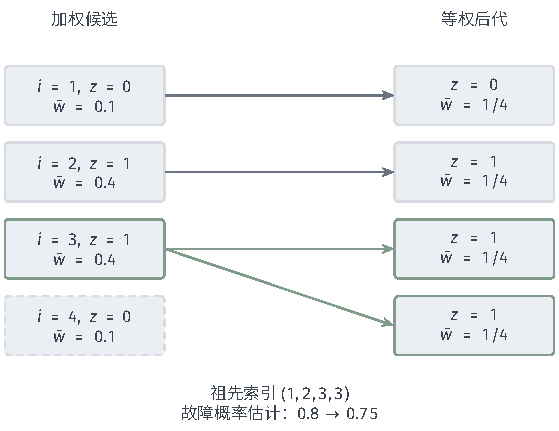
\includegraphics[width=94.650mm]{figures/06-probabilistic-graphical-models/02-inference/tikz/pgm-sampling-resampling/figure.pdf}
  \caption{二状态例子的系统重采样。左侧为四个带权候选，右侧为等权后代；连线标明复制来源。候选$4$没有后代，候选$3$被复制两次。后代等权，但状态及祖先多样性仍由复制来源决定。}
  \label{fig:pgm-sampling-resampling}
\end{figure}

若一次传播及似然计算成本分别为$C_{\mathrm{tr}},C_{\mathrm{obs}}$，一轮基础滤波成本约为$O(n(C_{\mathrm{tr}}+C_{\mathrm{obs}}))$，再加重采样成本。分层和系统法可沿累积权重单次扫描，在$O(n)$时间内完成；多项式法可用累积分布二分查找得到$O(n\log n)$实现，也有预处理后线性总成本的实现。只保存当前$d$维状态需$O(nd)$空间，保存所有粒子历史则随$T$增长。增加粒子数可改善固定时刻近似，长期平滑和高维滤波的效率还取决于路径与权重退化。

\subsection{Rao--Blackwell化粒子滤波}
\label{sec:pgm-sampling-rbpf}

粒子滤波对每个状态都要采样。若模型中一部分状态在给定其余状态时恰好有解析的条件分布（典型如离散模式下的连续状态服从线性高斯），就没必要也对它们采样——可以对这部分做精确Kalman递推，只对真正难处理的模式采样。这相当于在粒子滤波里再做一次Rao–Blackwell化。潜状态具有可解析的条件结构时，可以把随机计算集中到其余部分。\term{Rao--Blackwell化粒子滤波}（Rao--Blackwellized particle filtering, RBPF）只采样难以积分的状态部分，同时为每条粒子路径维护其余状态的条件分布。设$\bm{z}_t=(\bm{b}_t,\bm{u}_t)$，有
\begin{equation}
  \begin{aligned}
    &p(\bm{b}_{1:t},\bm{u}_t\mid\bm{x}_{1:t})\\
    &\qquad=p(\bm{b}_{1:t}\mid\bm{x}_{1:t})
        p(\bm{u}_t\mid\bm{b}_{1:t},\bm{x}_{1:t}).
  \end{aligned}
  \label{eq:pgm-sampling-rbpf-factor}
\end{equation}
若第二项可用有限维参数精确递推，则粒子只表示$\bm{b}_{1:t}$，每个粒子附带一份描述$\bm{u}_t$的解析状态。估计$h(\bm{b}_t,\bm{u}_t)$时，使用其条件期望
\[
  \widehat I_{t,h}^{\mathrm{RB}}
    =\sum_i\bar w_{t,i}
      \int h(\bm{b}_{t,i},\bm{u})
       p(\bm{u}\mid\bm{b}_{1:t,i},\bm{x}_{1:t})\,\mathrm{d}\bm{u}.
\]
查询中的条件分布已经使用当前观测$\bm x_t$，粒子加权却需要先计算看到该观测的概率。为区分这两个时刻，给定一条已扩展到$t$的模式路径，记
\[
  \begin{aligned}
    \pi_t^-(\bm u)
      &=p(\bm u_t=\bm u\mid\bm b_{1:t},\bm x_{1:t-1}),\\
    \ell_t(\bm b_{1:t})
      &=\int p(\bm x_t\mid\bm b_{1:t},\bm u)
                \pi_t^-(\bm u)\,\mathrm d\bm u.
  \end{aligned}
\]
这里$\pi_t^-$是当前观测进入之前的条件预测密度，$\ell_t$则是把连续状态积分掉后的预测观测密度。若$0<\ell_t<\infty$，看到$\bm x_t$后的条件密度才由Bayes公式给出：
\[
  \pi_t^+(\bm u)
    =\frac{p(\bm x_t\mid\bm b_{1:t},\bm u)\pi_t^-(\bm u)}
           {\ell_t(\bm b_{1:t})}.
\]
因此，查询积分使用$\pi_t^+$，权重计算使用$\pi_t^-$。把更新后的$\pi_t^+$再次当成预测分布来加权，会把同一次观测的影响重复算入。

模式路径本身也需要匹配提议。记模型在已有路径下的模式预测分布为
$a_t(\bm b_t)=p(\bm b_t\mid\bm b_{1:t-1},\bm x_{1:t-1})$，模式提议为$q_t^b(\bm b_t\mid\bm b_{1:t-1},\bm x_{1:t})$。对$t\geq2$，目标路径增加的因子为$a_t(\bm b_t)\ell_t(\bm b_{1:t})$，所以相应增量权重为
\[
  w_{t,i}\ \propto\ \bar w_{t-1,i}
    \frac{a_t(\bm b_{t,i})}
         {q_t^b(\bm b_{t,i}\mid\bm b_{1:t-1,i},\bm x_{1:t})}
    \ell_t(\bm b_{1:t,i}).
\]
比例常数在该轮粒子之间相同，重采样后的旧权重则按前述规则置为$1/n$。提议仍须覆盖有正目标贡献的模式；若模式按独立于连续状态的Markov链转移，则$a_t$简化为$p(\bm b_t\mid\bm b_{t-1})$。选择这一模式转移作为提议时，分式抵消，增量只剩积分预测似然；选择利用当前观测的其他模式提议时，分式必须保留。初始时刻同样使用模式先验与初始提议之比，并乘对应的初始积分观测密度。

典型例子是给定离散模式$b_t$后，连续状态服从线性高斯模型。每条模式路径维护高斯均值与协方差，通过Kalman递推完成条件滤波；模式仍用粒子表示。用标量的一步更新说明这一计算：给定某条模式路径及过去观测，连续状态预测分布为$U_t\sim\mathcal{N}(m^-,v^-)$，其中$v^->0$；观测满足$X_t=U_t+\varepsilon_t$，$\varepsilon_t\sim\mathcal{N}(0,\sigma_x^2)$，$\sigma_x^2>0$且噪声与$U_t$条件独立。预测观测是两个独立高斯量之和，故均值仍为$m^-$，方差为$v^-+\sigma_x^2$。这一步对未知$U_t$积分，也就是高斯卷积，得到用于模式权重的预测似然。

接着固定已经看到的$x_t$，更新连续状态。将先验预测密度与似然相乘，关于$u$的指数为
\[
  -\frac12\left[
       \left(\frac1{v^-}+\frac1{\sigma_x^2}\right)u^2
       -2\left(\frac{m^-}{v^-}+\frac{x_t}{\sigma_x^2}\right)u
       \right]+\text{与$u$无关的项}.
\]
因此，后验精度为$1/v_t=1/v^-+1/\sigma_x^2$，均值满足$m_t=v_t(m^-/v^-+x_t/\sigma_x^2)$。把分母通分，再把均值写成“预测均值加观测残差修正”的形式，便得到
\begin{equation}
  \begin{aligned}
    &p(x_t\mid b_{1:t},x_{1:t-1})
       =\mathcal{N}(x_t;m^-,v^-+\sigma_x^2),\\
    &k_t=\frac{v^-}{v^-+\sigma_x^2},\\
    &m_t=m^-+k_t(x_t-m^-),\qquad v_t=(1-k_t)v^-.
  \end{aligned}
  \label{eq:pgm-sampling-rbpf-gaussian}
\end{equation}
第一行对应观测前的积分预测似然，用于粒子权重；后两行给出观测后的条件高斯参数，用于查询和下一轮预测。$k_t$是标量Kalman增益，控制当前观测对条件均值的修正幅度：预测方差相对于观测噪声越大，当前残差得到的权重越大。上述卷积与配方承担不同计算，不能把观测后的条件高斯再次代入同一次预测似然。

假设两个等先验模式分别给出$U_t\sim\mathcal{N}(0,1)$和$\mathcal{N}(0,4)$，共同观测噪声方差$\sigma_x^2=1$，观测$x_t=1$。两模式的预测似然分别为$\mathcal{N}(1;0,2)\approx0.219696$和$\mathcal{N}(1;0,5)\approx0.161434$，归一化模式权重约为$0.576433,0.423567$。更新后的连续状态分别服从$\mathcal{N}(0.5,0.5)$和$\mathcal{N}(0.8,0.8)$，故混合均值约为$0.627070$。连续状态通过两个条件高斯表示，均值可直接积分，同时保留条件不确定性。从这些高斯额外抽样再估计均值，会引入额外的条件抽样波动。

RBPF利用可精确递推的条件分布减少随机性，但每个粒子需要存储协方差并进行矩阵运算，模式路径也可能退化。若用扩展Kalman等近似替代精确条件积分，结果中还包含条件滤波的近似误差。全方差公式解释相容条件化下的方差缩减；相同运行时间下的整体收益，则需比较粒子数、重采样和解析运算成本。Doucet等人的工作详细讨论了这一构造\scite{pgm-sampling-doucet2000}。

\section{算法分析}
\label{sec:pgm-sampling-analysis}

采样估计是否可信，需要同时说明目标、渐近规模与有限计算误差。渐近正确不代表有限时间内准确，不同机制的误差来源也不同：独立样本看权重和矩，MCMC看链的相关性与遍历性，粒子滤波还要看权重退化和祖先多样性。保持正确目标的核可能因探索缓慢而给出不可靠的有限估计，有有限样本偏差的比值估计也可能随样本数趋于一致。下面先逐一建立独立样本、加权样本、链与粒子的极限条件，再讨论能够从有限输出中直接检查的诊断量。

\subsection{一致性、偏差与方差}
\label{sec:pgm-sampling-consistency}

独立直接采样的条件最清楚。对固定查询$h$，独立同分布与$\mathbb{E}_p|h|<\infty$给出强一致性；$\mathbb{E}_p h^2<\infty$进一步给出式~\eqref{eq:pgm-sampling-iid-clt}的方差与中心极限定理。对于有界指示函数，这些矩条件自动成立。对于Cauchy等重尾分布，某些均值不存在，此时需要选择有定义的查询量。$n^{-1/2}$误差尺度也只描述随机计算误差，不包括模型失配。

重要性采样把这些矩条件移到了$q$下的加权函数。归一化目标的普通IS需要$r h$可积；有限方差与普通中心极限定理需要$\mathbb{E}_q(rh)^2<\infty$。SNIS的一致性条件见式~\eqref{eq:pgm-sampling-snis}之后。为了得到一个方便使用的SNIS中心极限定理，仍令候选独立来自固定$q$，要求目标支撑被覆盖、$0<Z_{\bm x}=\mathbb E_qw<\infty$，并进一步要求$\mathbb{E}_q w^2<\infty$和$\mathbb{E}_q(wh)^2<\infty$。

先把比值中同时变化的两部分写清。令$Y_i=w_i h(\bm z_i)$、$\bar Y_n=n^{-1}\sum_iY_i$与$\bar W_n=n^{-1}\sum_iw_i$，则$\widehat I_{h,n}^{\mathrm{SNIS}}=\bar Y_n/\bar W_n$，而$\mu_Y=\mathbb E_qY=Z_{\bm x}I_h$。记$\Delta_Y=\bar Y_n-\mu_Y$和$\Delta_W=\bar W_n-Z_{\bm x}$。联合中心极限定理使这两个偏差均为$O_{\mathbb P}(n^{-1/2})$；$\bar W_n$则依概率趋向严格正的$Z_{\bm x}$，所以分母为正的概率趋于$1$。有限样本的全零权重仍应按前文报告，不能输出归一化估计；讨论渐近分布时，可在这类事件上任意补定一个固定值，因为该事件概率趋零，不改变下面的分布极限。函数$f(a,b)=a/b$在该点对分子、分母的导数分别为$1/Z_{\bm x}$和$-I_h/Z_{\bm x}$，因而一阶展开为
\[
  \begin{aligned}
    \widehat I_{h,n}^{\mathrm{SNIS}}-I_h
      &=\frac{\Delta_Y-I_h\Delta_W}{Z_{\bm x}}
           +o_{\mathbb P}(n^{-1/2}),\\
    \Delta_Y-I_h\Delta_W
      &=\frac1n\sum_{i=1}^n w_i\bigl(h(\bm z_i)-I_h\bigr).
  \end{aligned}
\]
第二行利用$\mu_Y=Z_{\bm x}I_h$抵消常数项。它表明分母波动与分子波动共同形成中心化贡献，并且$\mathbb E_q[w(h-I_h)]=0$。对这个贡献应用独立样本中心极限定理，得到
\begin{equation}
  \begin{aligned}
    \sqrt n(\widehat I_{h,n}^{\mathrm{SNIS}}-I_h)
       &\xrightarrow{\mathrm{d}}\mathcal{N}(0,v_h^{\mathrm{IS}}),\\
    v_h^{\mathrm{IS}}
       &=\frac{\mathbb{E}_q[w^2(h-I_h)^2]}{Z_{\bm{x}}^2}.
  \end{aligned}
  \label{eq:pgm-sampling-snis-clt}
\end{equation}
关键的一阶随机量是$w(h-I_h)$，不是单独的$w$。这解释了为什么同一组权重对于不同查询可能具有不同精度。

SNIS的偏差也可由同一个比值展开看清，但这次需要控制取期望后的余项，只有一阶的依概率结论还不够。为简化书写，在以下展开中暂记$Z=Z_{\bm x}$。将$f(a,b)=a/b$在$(\mu_Y,Z)$处展开到二阶，得到
\[
  \begin{aligned}
    \widehat I_{h,n}^{\mathrm{SNIS}}-I_h
      &=\frac{\Delta_Y-I_h\Delta_W}{Z}\\
      &\quad-\frac{\Delta_Y\Delta_W}{Z^2}
         +\frac{I_h\Delta_W^2}{Z^2}+R_n,\\
    R_n&=\frac{\Delta_W^2(\Delta_Y-I_h\Delta_W)}
                  {Z^2\bar W_n}.
  \end{aligned}
\]
这里写出的$R_n$在$\bar W_n>0$时还是精确的余项表达。若在全零权重事件上将估计量补定为常数$c_0$，也应在该事件上把$R_n$定义为$c_0-I_h$。这是因为此时$\bar Y_n=\bar W_n=0$，已经显示的一阶和二阶项相互抵消，余项必须承接补定估计量与$I_h$的差。独立候选下，全零事件概率为$\mathbb P_q(w=0)^n$；由$\mathbb E_qw>0$可知$\mathbb P_q(w=0)<1$，所以这一补定对余项期望的贡献随$n$指数衰减，不改变下面的偏差阶。由于比值对分子线性，没有$\Delta_Y^2$项；分子与分母的交叉项带负号，反映分子固定时，分母增大会使比值减小。两个一次项的期望均为零，而独立候选给出
\[
  \mathbb E[\Delta_Y\Delta_W]
      =\frac{\operatorname{Cov}_q(wh,w)}n,\qquad
  \mathbb E[\Delta_W^2]=\frac{\operatorname{Var}_q(w)}n.
\]
在足够高阶矩和分母尾部控制使$\mathbb E R_n=o(n^{-1})$的条件下，对二阶展开取期望，便得到
\begin{equation}
  \mathbb{E}[\widehat I_{h,n}^{\mathrm{SNIS}}]-I_h
    =\frac{I_h\operatorname{Var}_q(w)-\operatorname{Cov}_q(wh,w)}
            {n Z_{\bm{x}}^2}+o(n^{-1}).
  \label{eq:pgm-sampling-snis-bias}
\end{equation}
例如$w\geq a>0$且$\mathbb{E}_q[w^4+|wh|^4]<\infty$，是控制分母和展开余项的一组较强充分条件。此时$\bar W_n\geq a$，两个样本均值偏差的二阶矩为$O(n^{-1})$、四阶矩为$O(n^{-2})$。将这些界代入$R_n$并使用Cauchy--Schwarz不等式，可得$\mathbb E|R_n|=O(n^{-3/2})=o(n^{-1})$。因此，常见的$O(n^{-1})$偏差来自交叉协方差与分母方差，而不是无条件的比值性质；这一阶数所需的余项和分母控制，比一致性所需的可积性与支持覆盖更强。

MCMC考察运行长度增长时的时间平均，其中样本通常相关。先说明强大数定律涵盖哪些起点。设固定的齐次转移核$K$在所声明的状态空间或闭合Harris类上正Harris常返，并保持概率分布$p$。对实值且满足$\mathbb E_p|h|<\infty$的$h$，从该类中的任意初始状态出发，时间平均都几乎必然收敛到$I_h$。这里“任意”限定在已经声明具有该性质的类内；仅知道某个核保持$p$，不足以把另一个封闭类中的起点也包括进来。非周期性另用于保证每一步的分布收敛；上述时间平均结论本身不要求非周期性。

若链从平稳分布启动，有限样本均值在期望存在时仍无偏，只是有相关性；从指定点启动时，有限预热用于减轻初值影响，剩余的初始化偏差还取决于核的混合速度。有限预热并不会把当前分布自动变成$p$，也不能替代一个结论所要求的起点条件。

MCMC中心极限定理还需额外条件。一组常用充分条件是\term{几何遍历性}（geometric ergodicity），即到平稳分布的距离按几何速率衰减，且允许系数依赖起点。具体地，在标准Borel状态空间上，设固定的齐次核$K$不可约、非周期且保持$p$，存在$0<a<1$及对$p$几乎处处起点有限的$C(\bm z)$，使
\[
  \lVert K^k(\bm z,\cdot)-p\rVert_{\mathrm{TV}}
    =\sup_B|K^k(\bm z,B)-p(B)|\leq C(\bm z)a^k.
\]
总变差距离在这里比较运行$k$步后的事件概率与目标事件概率，几何界控制两者相差的速率。标准Borel包括本章的欧氏空间及离散状态空间；这一可测性设定使常用条件分布和耦合论证能够适用。再要求某个$\delta>0$满足$\mathbb{E}_p|h|^{2+\delta}<\infty$，先从$\bm z^{(0)}\sim p$的平稳启动得到
\[
  \sqrt n(\widehat I_{h,n}-I_h)
     \xrightarrow{\mathrm{d}}\mathcal{N}(0,v_h^{\mathrm{MC}}).
\]
在上述一般几何遍历条件下，这个结论还可以扩展到$p$几乎处处的固定起点。这里允许排除$p$概率为零的异常起点。若进一步采用前面整类正Harris常返的设定，并保持非周期性，则该类中的每个起点都在总变差下收敛到$p$；将其与平稳链耦合，同一中心极限定理便可扩展到类内全部起点。这个扩展依据的是核在整类上的遍历性质，不是已经完成了有限预热。未被声明为该类成员的其他指定点，不能自动继承这个保证。

长期依赖的控制是推导正态误差分布所需的环节。再生方法把路径在特定随机返回时刻切成可以独立处理的完整区段，再控制初末不完整区段；Poisson方程方法则把中心化求和转为鞅差求和及可忽略的边界项，其中每个鞅差增量在给定过去信息时的条件均值为零。两者都需要证明相应矩和余项条件，不能只靠目标不变性得到正态误差。其他条件组合也可能建立中心极限定理，本章保留上述一组充分条件；更一般的证明以及从平稳启动扩展到$p$几乎处处固定起点的论证，见Roberts与Rosenthal的综述\scite{pgm-sampling-roberts2004}

SMC的样本数极限又不同：通常先固定一个有限时刻$t$，再令粒子数$n\to\infty$。为看清这一区别，可以考察一组较强而易检查的充分条件：初始粒子独立来自模型初始分布，传播使用正确的Markov转移；每个固定时刻的观测似然作为状态函数有正下界和有限上界；测试函数$h$有界；采用固定日程的多项式重采样。此时滤波积分估计一致，并满足适当的$\sqrt n$中心极限定理。一般提议需要相应的重要性权重矩条件，其他重采样方案和自适应日程还需要各自的方差与依赖条件，后代数条件无偏只是其中一项要求。

固定时刻一致性的证明思路是归纳。给定旧粒子后，新传播条件独立，因此对有界函数，传播抽样相对于其条件均值的方差为$O(1/n)$。条件均值是旧经验分布对转移后函数的积分，由归纳假设收敛。乘有界似然并除以远离零的归一化常数，仍保持收敛；多项式重采样再增加一个由式~\eqref{eq:pgm-sampling-resampling-variance}控制的$O(1/n)$条件方差。固定步数下反复使用这三个步骤便得到一致性。这是证明纲要，中心极限定理还需追踪每一代随机扰动如何传播，渐近方差包含历史各代贡献，而不只是当前粒子的样本方差\scite{pgm-sampling-chopin2004}

上述证明中的误差常数可以随$t$迅速增大。固定$n$让时间无限延长，与固定$t$让$n$趋向无穷，是不同的极限；要获得时间一致误差界，通常还需状态转移的遗忘或混合性质，以及适当的似然控制。归一化粒子滤波均值一般有有限$n$偏差。边缘似然却可以有无偏的粒子估计，因为它保留的是未归一化积分，而不是随机分母下的比值。

先把需要保存的尺度接回算法~\ref{alg:pgm-sampling-bootstrap}。记$g_t(\bm z)=p(\bm x_t\mid\bm z)$，传播后、归一化前的权重为$w_{t,i}=v_i g_t(\bm z_{t,i})$，其中$v_i$就是算法中的旧归一化权重，初始时为$1/n$。每轮归一化除掉的总和为
\begin{equation}
  \begin{aligned}
    \widehat c_t&=\sum_{i=1}^n v_i g_t(\bm z_{t,i}),\\
    \widehat Z_t&=\prod_{s=1}^t\widehat c_s,\qquad \widehat Z_0=1.
  \end{aligned}
  \label{eq:pgm-sampling-evidence-product}
\end{equation}
$\widehat c_t$近似预测观测密度$p(\bm x_t\mid\bm x_{1:t-1})$，$\widehat Z_t$近似边缘似然$p(\bm x_{1:t})$。初始时刻及上一轮已经重采样时$v_i=1/n$，因子是当前似然的粒子平均；上一轮未重采样时必须继续使用保留的非等权$v_i$。只保存归一化权重会丢掉这些总和。若为数值稳定对全部权重乘了共同尺度，计算$\widehat c_t$时还须还原该尺度，或在对数域保存对应的加数。

乘积的无偏性不能由“各因子分别无偏”推出，因为各轮使用的粒子相互依赖。可以直接对未归一化经验积分作条件递推。固定有限时刻和粒子数，先考虑初始独立模型采样、正确模型转移及每轮多项式重采样。观测似然非负有界、查询$h$有界，是使以下期望与积分均存在的一组充分条件。先约定：仅在截至当前每轮总权重都为正的存活事件上定义归一化经验积分；若某轮总权重为零，则直接把该运行的$\widehat Z_t$和$\Gamma_t^n(h)$定义为零，并在后续各轮维持为零，避免用零乘一个未定义的归一化积分。在存活分支上，令$\eta_t^n(h)$表示完成本轮可选重采样后的经验积分，$\Gamma_t^n(h)=\widehat Z_t\eta_t^n(h)$；未重采样时仍使用原来的加权积分。给定传播后的粒子，条件无偏的重采样使$\eta_t^n(h)$的条件均值等于$\sum_i\bar w_{t,i}h(\bm z_{t,i})$。因此，复制前的未归一化积分为
\[
  \widehat Z_{t-1}\sum_i v_i g_t(\bm z_{t,i})h(\bm z_{t,i}),
\]
复制后的$\Gamma_t^n(h)$在当前粒子信息下的条件期望与它相同；其中$\widehat c_t$恰好消去了归一化权重中的随机分母。对$t\geq2$，再对本轮传播取条件期望，有
\begin{equation}
  \begin{aligned}
    \mathbb E[\Gamma_t^n(h)\mid\mathcal F_{t-1}]
      &=\widehat Z_{t-1}\sum_i\bar w_{t-1,i}
          Q_t h(\bm z_{t-1,i}),\\
    Q_t h(\bm z)
      &=\int p(\bm z'\mid\bm z)g_t(\bm z')
                    h(\bm z')\,\mathrm d\bm z'.
  \end{aligned}
  \label{eq:pgm-sampling-evidence-recursion}
\end{equation}
这里$\mathcal F_{t-1}$包含上一轮重采样后的全部信息，$Q_t h$把一次状态转移、观测加权和当前查询合成一个旧状态的函数。含粒子状态与归一化权重的和式在对应存活分支上使用；若上一轮已经灭绝，递推两端都按零定义，无需再生成后续粒子。右侧正是$\Gamma_{t-1}^n(Q_t h)$。初始独立采样给出$\mathbb E\Gamma_1^n(h)=\int p(\bm z_1)g_1(\bm z_1)h(\bm z_1)\,\mathrm d\bm z_1$。据此逐轮取期望，便得到
\[
  \begin{aligned}
    \mathbb E\Gamma_t^n(h)
      &=\int h(\bm z_t)p(\bm z_t,\bm x_{1:t})\,\mathrm d\bm z_t,\\
    \mathbb E\widehat Z_t&=p(\bm x_{1:t}).
  \end{aligned}
\]
第二行取$h\equiv1$。它证明的是未归一化估计的无偏性；$\Gamma_t^n(h)/\widehat Z_t$仍有随机分母，因而不能据此判定滤波均值有限样本无偏。

若某轮权重全零，则当前滤波分布无法归一化，算法按原规则报告退化并停止。为了把证据估计定义在所有随机运行上，可将这种运行的$\widehat Z_t$及后续$\widehat Z_s$记为零，未归一化经验积分也记为零；此时不再要求定义对应的归一化滤波估计。零贡献必须保留在重复运行的平均中，不能丢弃失败运行、只对成功运行求平均后仍声称无偏。此前的一致性示例使用严格正下界，已经排除了全零事件；此处非负有界的设定则容许它出现。

按当前已有粒子信息决定是否重采样，例如算法中的权重ESS阈值，只要决策不使用未来随机量，且所选方案在该信息条件下仍保持后代均值，重采样或不重采样都保持同一个经验积分的条件期望，上述无偏递推仍可逐步应用。这个论证固定粒子数和要估计的时刻；任意改变粒子数、停止时刻、提议或目标的自适应规则需要重新核对权重与条件期望。即使某种自适应重采样保留了证据无偏性，其中心极限定理和方差公式也仍须满足该规则的额外条件。

\subsection{有效样本量与收敛诊断}
\label{sec:pgm-sampling-diagnostics}

估计精度既取决于样本数量，也取决于样本如何贡献以及如何相关。\term{有效样本量}（effective sample size, ESS）借独立样本的尺度描述这些影响。权重ESS衡量贡献集中，自相关ESS匹配具体查询的长期方差，两者需要分别解释。

先只考察归一化非负权重如何分配本批贡献。若恰有$m$个粒子各占$1/m$、其余为零，则平方权重和为$m(1/m)^2=1/m$，取倒数正好返回贡献相等的粒子数$m$。更一般地，按权重独立抽取两次索引，两次选中同一原粒子的概率为$\sum_i\bar w_i^2$。这一概率越大，权重越集中；其倒数用“等贡献粒子数”的尺度表示集中程度。由此引出常用的\term{权重有效样本量}（weight-based ESS）
\begin{equation}
  n_{\mathrm{eff}}^{w}
    =\frac{1}{\sum_i\bar w_i^2}
    =\frac{(\sum_i w_i)^2}{\sum_i w_i^2},
  \qquad 1\leq n_{\mathrm{eff}}^{w}\leq n.
  \label{eq:pgm-sampling-weight-ess}
\end{equation}
上下界来自非负性和Cauchy--Schwarz不等式：等权时等于$n$，一个权重占满总和时等于$1$。若候选确实独立来自固定$q$且$\mathbb{E}_q w^2<\infty$，大数定律还给出
\[
  \frac{n_{\mathrm{eff}}^{w}}{n}
    \longrightarrow
    \frac{(\mathbb{E}_q w)^2}{\mathbb{E}_q w^2}
    =\frac{1}{1+\operatorname{CV}_q(w)^2},
\]
其中$\operatorname{CV}_q(w)$为权重的标准差与均值之比。因此，权重ESS描述已抽到的贡献集中程度；对具体$h$的方差等价样本数，还需考虑函数值与权重的关系。真正的IS渐近方差还含有式~\eqref{eq:pgm-sampling-snis-clt}中的$(h-I_h)^2$。

表~\ref{tab:pgm-sampling-weight-example}中，$n_{\mathrm{eff}}^w=2.51^2/(0.01^2+0.9^2+0.9^2+0.7^2)\approx2.986$。这一数值只反映已抽到的权重，未访问的罕见状态仍需其他检查。粒子滤波例子重采样前的权重ESS为$1/(0.1^2+0.4^2+0.4^2+0.1^2)\approx2.941$，重采样后立即变成$4$；但图~\ref{fig:pgm-sampling-resampling}已经显示祖先反而减少。在SMC中，权重ESS主要帮助选择重采样时刻，滤波误差还需要考虑状态和祖先多样性。

MCMC常常所有样本等权，权重ESS因而为$n$。重复停留和缓慢移动带来的时间相关，需要通过样本均值的协方差分析。设链已平稳，$0<\sigma_h^2=\operatorname{Var}_p(h)<\infty$，令$\rho_h(\ell)$为$h(\bm{z}^{(k)})$与$h(\bm{z}^{(k+\ell)})$的相关系数。展开样本均值的协方差和，有
\begin{equation}
  \operatorname{Var}(\widehat I_{h,n})
    =\frac{\sigma_h^2}{n}
      \left[1+2\sum_{\ell=1}^{n-1}
          \left(1-\frac{\ell}{n}\right)\rho_h(\ell)\right].
  \label{eq:pgm-sampling-autocorrelation-variance}
\end{equation}
滞后$\ell$的样本对恰有$n-\ell$个，因而出现括号中的系数。若自相关绝对可和，定义\term{积分自相关时间}（integrated autocorrelation time）
\begin{equation}
  \tau_h=1+2\sum_{\ell=1}^{\infty}\rho_h(\ell),\qquad
  v_h^{\mathrm{MC}}=\sigma_h^2\tau_h,\qquad
  n_{\mathrm{eff},h}^{\mathrm{MC}}=\frac{n}{\tau_h}.
  \label{eq:pgm-sampling-mcmc-ess}
\end{equation}
这里假定$0<\tau_h<\infty$；还需前述中心极限定理条件，才能据此使用正态近似误差区间。$\tau_h$依赖函数$h$，故均值、尾概率和不同坐标通常有不同ESS；负相关还可能使$\tau_h<1$，此时ESS大于$n$，并不矛盾，因为它匹配的是估计方差而非独立点的实际数量。

例如平稳自回归序列的$\rho_h(\ell)=0.9^\ell$，则$\tau_h=1+2(0.9/0.1)=19$，$10000$次迭代对该查询只有约$526$个独立样本的渐近精度。对前述强相关高斯的Gibbs坐标，$\rho=0.99$给出的每轮相关系数为$0.9801$，对应$\tau_h=(1+0.9801)/(1-0.9801)\approx99.50$。两个例子将运行长度与该查询的渐近精度联系起来，高接受率仍可能伴随低有效样本量。简单地每隔若干步保留一个点虽然降低保留序列的相关性，也丢弃了已付费的计算；除非有存储或后续处理约束，稀疏保留不是改善采样效率的通用办法。

样本相关系数的高滞后估计噪声较大，不能把所有可计算滞后的样本相关系数直接相加。截断方法只累计到预先选定或按稳定规则选出的滞后，再检查截断位置改变时结论是否稳定；谱方差方法对样本自协方差施加随滞后衰减的窗权重，估计零频率处的长期波动尺度。批均值方法则把序列分成若干连续长批，使每批内部的相关都进入批均值，再用批间波动估计长期方差。

例如将$n$个保留的$h$值分为$a$个长为$b$的等长批，暂设$n=ab$，$a\geq2$。记第$j$批均值为$\bar H_j$、总均值为$\bar H$，可构造
\[
  \widehat v_h^{\mathrm{MC}}
    =\frac{b}{a-1}\sum_{j=1}^a(\bar H_j-\bar H)^2.
\]
若单批已经足够长，批均值的方差约为$v_h^{\mathrm{MC}}/b$，所以样本批方差乘以$b$对应所需的长期方差尺度。渐近使用时应让批长和批数都增长，并满足相应遍历与矩条件；前述中心极限定理本身不自动保证任意截断、窗宽或批长规则都一致。用$\sqrt{\widehat v_h^{\mathrm{MC}}/n}$报告具体查询的MCSE，可以把估计出的长期方差直接换回该查询的均值误差，而不是只报告一个全局ESS。

独立SNIS可以对式~\eqref{eq:pgm-sampling-snis-clt}作样本代入。在该式的覆盖与二阶矩条件下，以$\bar W_n$代替$Z_{\bm x}$、以$\widehat I_h$代替$I_h$，把期望代为样本平均，得到
\[
  \begin{aligned}
    \frac{\widehat v_h^{\mathrm{IS}}}{n}
       &=\frac{n^{-1}\sum_iw_i^2(h_i-\widehat I_h)^2}
               {n\bar W_n^2}\\
       &=\sum_i\bar w_i^2(h_i-\widehat I_h)^2,\\
    \widehat{\operatorname{MCSE}}(\widehat I_h)
       &=\left[\sum_i\bar w_i^2(h_i-\widehat I_h)^2\right]^{1/2},
       \qquad h_i=h(\bm z_i).
  \end{aligned}
\]
这里依赖候选独立与相应加权矩；若权重重尾到没有所需方差，代入一个有限数值不能恢复中心极限定理。共享祖先的粒子系统还包含额外依赖，不能直接把独立SNIS的式子当作其全部误差。SMC可通过多次独立运行整个粒子滤波比较估计波动，或采用专门的粒子方差估计。

单条链可能在一个局部区域内看起来很稳定。多链诊断从分散的有效初值运行若干条独立链，比较链内与链间变化。\term{$\widehat R$诊断}（R-hat diagnostic）用两种变化尺度之比发现不同链尚未探索相同分布的迹象。设共有$m\geq2$条链，每条保留$n\geq2$个函数值$h_{j,k}$，链均值为$\bar h_j=n^{-1}\sum_kh_{j,k}$，总体均值为$\bar h=m^{-1}\sum_j\bar h_j$，链内样本方差采用
\[
  s_j^2=\frac1{n-1}\sum_{k=1}^n(h_{j,k}-\bar h_j)^2.
\]
这里$n$表示每条链的保留长度，不是多条链合计长度。经典形式先计算链内平均方差$W$和按$n$放大后的链均值样本方差$B$，再构造
\begin{equation}
  \begin{aligned}
    W&=\frac1m\sum_{j=1}^{m}s_j^2,&
    B&=\frac{n}{m-1}\sum_{j=1}^{m}(\bar h_j-\bar h)^2,\\
    \widehat V&=\frac{n-1}{n}W+\frac{B}{n},&
    \widehat R&=\sqrt{\widehat V/W}.
  \end{aligned}
  \label{eq:pgm-sampling-rhat}
\end{equation}
$B/n$是各链均值之间的样本方差，$B$与$W$则都以单个函数值的方差为尺度。若各链已经近似探索同一分布且相关较弱，链均值方差约为单点方差除以$n$，所以$B$与$W$应大致相当；若链还停留在不同区域，链均值差异就可能使$B$明显增大。$\widehat V$将链内估计乘$(n-1)/n$，再补入链均值差异$B/n$，因而能够暴露只看链内波动遗漏的位置差异。样本相关与有限长度会影响这些估计，不能要求每次运行都恰有$\widehat R=1$。

该比值的通常解释要求$W>0$。所有链完全不动而使$W=0$时，比值无定义或缺少通常的尺度比较含义，应先检查链的移动，而不能将常数输出当成已经充分探索。

秩归一化的分裂诊断先把每条链的保留序列分成前后两半，并把各半段当成单独链。两半的位置差异因而能进入链间比较，帮助发现链内漂移；每半段仍需至少两个值，长度为奇数时可舍去中间一个值以保持两半等长。随后将全部半链样本合并排序，对并列值使用平均秩。若合计有$S$个值、某个值的秩为$r$，用$\Phi^{-1}((r-3/8)/(S+1/4))$将它映射为标准正态分位数，其中$\Phi$是标准正态分布函数。将变换后的值放回各自半链，按式~\eqref{eq:pgm-sampling-rhat}计算秩归一化的分裂$\widehat R$。这一变换保留排序信息，减轻原始重尾值对方差估计的影响。

位置相近的链仍可能具有不同尺度。为检查这一点，再计算每个原始样本到合并中位数的绝对偏差，对这些折叠值重新取秩、映射为正态分位数并计算分裂$\widehat R$。最终报告原始秩归一化分裂值与折叠后的值中的较大者，使位置或尺度差异中的任一种都能触发检查。

多链ESS还需要把每条链的时间相关与链间差异合在一起，不能简单相加各链单独报告的ESS。对当前要诊断的序列，仍以$m$表示半链数、$n$表示每条半链长度，并按式~\eqref{eq:pgm-sampling-rhat}重新计算$s_j^2,W,\widehat V$。沿第$j$条半链，用除数$n$计算各滞后的样本自协方差，再除以该链滞后零的自协方差，得到$\widehat\rho_{j,\ell}$。一种常用合并方式为
\begin{equation}
  \begin{aligned}
    \widehat\rho_\ell
      &=1-\frac{W-m^{-1}\sum_j s_j^2\widehat\rho_{j,\ell}}
                     {\widehat V},\\
    \widehat\tau&=1+2\sum_{\ell=1}^{L}\widehat\rho_\ell,\qquad
    \widehat n_{\mathrm{eff}}=\frac{mn}{\widehat\tau}.
  \end{aligned}
  \label{eq:pgm-sampling-multichain-ess}
\end{equation}
这里$L<n$是相关和的截断滞后，不是HMC的积分步数。若各链已经充分混合，使$\widehat V$与$W$接近，合并式近似对各链自相关按方差加权；若链均值差异使$\widehat V$增大，合并相关也随之增大，从而降低ESS。方差为零的单条半链不定义其相关系数，而把该链的自协方差贡献$s_j^2\widehat\rho_{j,\ell}$记为零；若合并方差也为零，则应报告退化并检查序列。

实际求和时，仍需避免高滞后噪声。常用做法将滞后$0,1$、$2,3$等相邻相关系数成对求和，保留从开头起连续为正的成对和；也可将后一个成对和限制为不大于前缀最小值，再整理为式~\eqref{eq:pgm-sampling-multichain-ess}的相关和。这给出初始正序列及其单调调整的截断规则。它们的理论性质与核的条件有关，不能把对任意短序列的数值输出当成已验证的长期方差；若估出的$\widehat\tau$非正或对截断极不稳定，应先检查运行长度和探索。总样本数在这里为$mn$，而不是任意一条半链的长度。

\term{主体ESS}（bulk ESS）根据秩变换后的序列，经上述合并与截断衡量主体区域的探索，却不直接给出原始均值的MCSE。\term{尾部ESS}（tail ESS）则针对两端分位的累计概率。令$\widehat q_\alpha$为合并样本的$\alpha$分位数，分别对$\alpha=0.05$和$0.95$构造沿链排列的指示序列$\mathbb{I}\{h_{j,k}\leq\widehat q_\alpha\}$，按同一多链合并与截断步骤分别计算两组序列的ESS，并取两个ESS的较小值。这些序列表示“落在分位阈值以下”的累计事件，不是“落在分位点附近某个小区间”的事件；上端累计事件也可取补集表示上尾，其相关结构相同。分位数误差还涉及分位处密度等条件，尾部ESS提供相应累计概率的探索诊断，不能代替所有尾部查询的精度分析。

原始均值和其他非线性查询的MCSE仍需按相应函数单独估计。常用的$\widehat R<1.01$是经验筛查标准，用于判断有限输出是否暴露出明显的多链差异；它不是已经收敛的证明。上述秩、折叠与尾部诊断的构造见Vehtari等人的论文\scite{pgm-sampling-vehtari2021}

有限输出的诊断可以共同检查多链轨迹、秩分布、查询函数的MCSE、主体和尾部ESS；HMC还需检查能量误差、积分失败与长时间拒绝。若所有链都局限于同一个模态，这些量仍可能正常。使用分散的有效初值，增加预算，检查模型几何，并与可解析特例或独立算法比较，有助于发现部分遗漏。诊断提供有限探索的证据，其范围仍受已访问区域限制。

\subsection{方法选择与计算边界}
\label{sec:pgm-sampling-choice}

采样器选择应从具体模型可计算的部件出发，而不是从方法的流行程度出发。若已有准确且廉价的直接采样器，独立平均通常最容易分析和并行；只有联合采样器而证据并不稀有时，拒绝采样能得到独立后验样本。若能够构造充分覆盖目标的提议，重要性采样便于并行且可估计归一化常数，但应优先检查权重尾部，而非仅拟合后验峰附近。

若只有未归一化密度及局部条件，MCMC可以避免全局提议的要求。满条件易抽样且相关适中时，Gibbs利用图结构获得低成本更新；强相关变量应考虑分块、折叠或重新参数化。连续密度可微时，HMC能用较贵的一次轨迹换取更远移动，但高维离散结构、多峰分离或复杂约束可能需要其他构造。若目标随新观测递推，粒子滤波直接复用过去计算；存在条件线性高斯部分时，RBPF可以把预算集中到真正需要采样的状态。

实际比较应固定查询与计算预算。一个每步便宜但高度相关的链，可能比一个每步较贵的链花更多时间才能达到同样MCSE。独立重要性采样虽可并行生成候选，若少数极端权重支配估计，多数候选对该查询的有效贡献仍然很小；独立MH则可能在到达高权重状态后长时间拒绝普通候选，表现为相关的重复停留。这两种损失分别通过贡献集中与链的时间依赖发生，不能只因都使用独立提议就混为同一种误差。因此应比较具体查询的MCSE随时间变化，或该查询的ESS每秒，并把预热、提议构造、梯度和解析积分计入成本。模型中的条件独立性帮助局部计算，却不保证后验中的统计相关很弱。

变分推断在可优化分布族中选择后验近似（第~\ref{chap:pgm-variational}章），采样则用随机经验表示估计后验积分。两者分别具有表达、求解和有限计算误差，表~\ref{tab:pgm-sampling-vi-comparison}在同一后验任务下比较这些因素。

\begin{table}[htbp]
  \centering
  \begin{tabularx}{\linewidth}{@{}lXX@{}}
    \toprule
    方面 & 采样近似 & 变分近似\\
    \midrule
    渐近目标 & 在相应覆盖、矩与遍历条件下，可逼近原后验积分 & 受分布族与目标函数限制，充分优化后仍可能有近似误差\\
    有限预算 & 有抽样波动，SNIS与非平稳MCMC等还可能有偏差 & 有分布族误差、优化误差，随机优化也有波动\\
    后验覆盖 & 漏模态、权重退化或慢混合会破坏有限样本覆盖 & 某些族与散度倾向集中于局部区域；覆盖行为取决于具体族与目标\\
    并行与规模 & 独立候选、多链和粒子可并行；单链有顺序依赖，重采样需同步 & 易利用小批量和摊销网络，但依赖相应模型与优化结构\\
    精度判断 & 查询相关的标准误与多种诊断并用 & 目标函数改善不等于所有后验查询都已准确\\
    \bottomrule
  \end{tabularx}
  \caption{在同一后验推断任务上比较采样与变分。渐近保证都有适用条件，有限预算下均需检查遗漏的后验结构。}
  \label{tab:pgm-sampling-vi-comparison}
\end{table}

两类方法还可以结合。拟合的变分分布可作为重要性采样或独立MH的提议，其支持覆盖与权重尾部决定后续校正和探索的效果。小规模、可高精度采样的问题则可提供变分误差的参照。具体方案需要在相同查询、计算预算和误差要求下比较。

\Needspace{8\baselineskip}
\section{本章小结}
\label{sec:pgm-sampling-summary}

采样推断用样本统计量估计后验概率和期望。独立候选通过目标生成、接受规则或权重匹配后验；Markov链通过保持目标的转移及充分探索计算时间平均；粒子系统通过传播、加权和后代分配追踪变化的目标。设备报警例说明，先验候选与后验候选回答不同的概率查询，相应的条件化或权重是得到所需答案的环节。

HMC以动量刷新、可逆保体积积分和Metropolis校正形成完整的后验更新。刷新改变轨迹方向和能量，可逆积分构造可配对的提议，末端校正处理离散能量误差。粒子滤波则以重采样把后续计算集中于高权重路径，但复制可能减少状态和祖先的多样性。两种方法均需将保持目标的构造与实际探索的效率分别检查。

误差分析与查询量和渐近条件对应。独立样本使用可积性与有限矩，重要性采样检查支持覆盖和加权矩，MCMC检查遍历及长期依赖，SMC通常先固定时间再增加粒子。权重ESS描述本批贡献集中，自相关ESS匹配具体函数的长期方差，多链诊断检查探索是否一致。可解析特例、查询相关的标准误和针对失效方式的诊断，为有限计算结果提供互补证据。

到这里，精确消元、变分优化和随机采样都在给定模型下回答查询。若局部概率本身还未知，后验期望便会进入参数更新，推断误差也可能影响学习结果。第~\ref{chap:pgm-parameter-learning}章接着说明这种依赖何时出现，以及观测完整且不含潜变量时为什么有些模型能免去内层推断。

\paragraph{扩展阅读}
Murphy的教材可用于扩展重要性采样和Markov链方法。进一步阅读时，可分别考察目标不变性、遍历条件、有限步混合以及查询相关的估计方差，理解接受率和轨迹形状为何只反映其中一部分性质\scite{pgm-murphy2012}。

\chapter{参数学习}
\label{chap:pgm-parameter-learning}

到此为止，图的结构和每个局部分布的数值都被当作已知，前八章解决的是“模型给定后怎样做推断”。但这些局部概率（故障率是多少、过热条件下报警有多可能）并不会凭空得到，它们通常要从一批历史设备记录中估计出来。这就是第三部分“学习”的主题，本章先处理其中最基础的\emph{参数学习}：图结构和局部分布的形式（用哪种表、哪种高斯）已经定好，只缺里面的数值参数。设备故障模型$F\to H\to A\leftarrow S$规定了故障、过热、报警和传感器失灵之间的概率分解；要用它预测，还需确定故障率、过热条件概率等局部参数。前面的推断将参数视为已知，本章根据一批设备记录估计参数。

学习的难易首先取决于数据“看得到多少”。所有变量都已记录时，有向模型的参数往往只需数一数各种组合出现多少次，连续情形则退化为局部回归；一旦存在模型主动引入却从未观测的潜在状态，或某些本该记录的字段漏记了，就无法直接计数——此时每更新一次参数，都要先推断这些未观测量的后验分布、用“软计数”代替真实计数，学习于是和前两部分的推断耦合在一起。其次取决于想要什么形式的答案：是给出一个最合适的参数值（点估计），还是给出参数的整个后验分布、把“参数本身有多不确定”也保留下来。这两条选择相互正交、可以组合。后文先说明因子分解与归一化如何决定学习所需的统计量，再讨论潜变量和缺失值怎样引入推断，最后说明参数不确定性如何进入预测。

\section{参数学习的定义}
\label{sec:pgm-parameter-learning-definition}

本节固定学习问题的记号和两种基本准则，后续各节在不同数据可见性下落实它们。设$\mathcal{G}=(V,E)$为固定图，$d=|V|$。记全部节点随机变量为$\bm{W}=(W_1,\ldots,W_d)^\top$，按照数据设计，将其划分为直接记录的字段$\bm{X}$与模型主动设置的潜变量$\bm{Z}$，即在固定排列下$\bm{W}=(\bm{X}^\top,\bm{Z}^\top)^\top$。局部条件分布或势函数由参数向量$\bm{\theta}\in\Theta$控制。可行域$\Theta$包含参数维度以及概率和为$1$、方差为正、配分函数有限等约束。\term{参数学习}（parameter learning）利用记录在这一固定模型族内估计参数点或参数后验。边、潜变量与局部分布族的选择属于模型结构问题，本章把这些选择作为学习的前提。

\term{观测变量}（observed variable）是在当前数据获取设计中直接记录的模型变量，\term{潜变量}（latent variable）则是模型为了表达未观测状态而主动引入的随机量。\term{缺失值}（missing value）指本应记录、却在某条记录中未取得的字段值，它描述数据单元的状态。控制变量分布的参数$\bm{\theta}$则属于估计对象：MLE与MAP将其视为未知的固定优化量，分布估计用先验和后验描述其不确定性。这三个对象分别回答变量如何获取、某个值是否取得，以及分布参数如何估计。

本章用\term{观测完整}表示$\bm{X}$中原定记录的字段均已取得。因此，观测完整且不含潜变量时，每条记录给出全部模型变量；观测完整但含潜变量时，$\bm{X}$没有漏记，$\bm{Z}$仍按模型设定不可见；观测缺失时，$\bm{X}$还要按实际缺失模式拆成已观测部分与缺失部分。潜变量和缺失字段都通过求和或积分从观测似然中消去；缺失字段还涉及值为何未被记录的问题。

以观测完整且不含潜变量的独立记录为例，数据集记为$\mathcal{D}=\{\bm{x}_j\}_{j=1}^n$，其中$x_{j,i}$是第$j$条记录中节点$i$的取值。默认不同记录在给定共同参数后独立同分布，因而$p_{\bm{\theta}}(\mathcal{D})=\prod_jp_{\bm{\theta}}(\bm{x}_j)$。独立性作用于不同完整记录，一条记录内部的节点依赖仍由图描述。同一设备的连续时间观测可能相关，可用第~\ref{chap:pgm-dynamic}章的序列模型或另行处理时间相关性。

局部分布可以使用不同参数块，也可以共享参数。\term{参数共享}（parameter sharing）让多个节点或多条记录使用同一个未知参数，例如同型号传感器共用误报率。同一个共享参数受所有使用位置的局部项约束，估计时应汇总这些项共同优化。逐节点的独立最优值只有满足共享约束时才能构成可行解。

确定了数据记号后，还要规定“什么样的参数算好”。最常用的准则是看这批数据在该参数下出现的可能性有多大：让观测数据的（对数）似然最大的参数称为极大似然估计；若还对参数事先有偏好（先验），就把先验密度也加进去一起最大化，得到极大后验估计。MLE以数据似然比较候选参数，MAP再加入先验密度。令$\ell(\bm{\theta})=\log p_{\bm{\theta}}(\mathcal{D})$。在最优解存在时，两种点估计分别求解
\begin{equation}
  \begin{aligned}
    \widehat{\bm{\theta}}_{\mathrm{ML}}
      &\in\argmax_{\bm{\theta}\in\Theta}\ell(\bm{\theta}),\\
    \widehat{\bm{\theta}}_{\mathrm{MAP}}
      &\in\argmax_{\bm{\theta}\in\Theta}
        \{\ell(\bm{\theta})+\log p(\bm{\theta})\}.
  \end{aligned}
  \label{eq:pgm-parameter-learning-point-objectives}
\end{equation}
似然固定数据后随参数变化，MAP的密度及众数还依赖参数坐标与基准测度。非线性换坐标时，Jacobian进入密度变换。候选集上的最优点可能不唯一；目标也可能只有上确界，因而需要先判断解是否存在（相关统计基础可参考\BookChapterRef{chap:statistical-inference}{卷2《数学准备：概率、因果与决策》的“统计推断”章}）。

MLE和MAP最终都只给出一个参数值，相当于认定“这就是最合适的参数”。但数据有限时，往往有多组参数都与观测相容；要把这种不确定性也保留下来用于预测，就要转而估计参数的后验分布，这就是贝叶斯式的基于分布估计的参数学习。若预测还需要反映多组参数与数据相容的程度，可采用\term{基于分布估计的参数学习}，保留
\begin{equation}
  p(\bm{\theta}\mid\mathcal{D})
  =\frac{p_{\bm{\theta}}(\mathcal{D})p(\bm{\theta})}
  {\int_\Theta p_{\bm{\vartheta}}(\mathcal{D})
    p(\bm{\vartheta})\,\mathrm{d}\bm{\vartheta}},
  \label{eq:pgm-parameter-learning-parameter-posterior}
\end{equation}
分母有限且为正时，先验与数据共同为各参数分配后验权重。这里的随机对象是参数$\bm{\theta}$；固定参数下的变量后验$p_{\bm{\theta}}(\bm{Z}\mid\bm{X})$则用于恢复未观测统计量，两者在学习中承担不同职责。后验均值$\mathbb{E}[\bm{\theta}\mid\mathcal{D}]$在相应平方损失下给出贝叶斯点估计，它是整个参数分布的一项摘要，通常与MLE、MAP不同。

训练准则决定哪些数据分布受到约束。把一条记录分成输入$\bm{x}_j$与输出$\bm{y}_j$后，联合训练与条件训练分别使用
\[
  \begin{aligned}
    \ell_{\mathrm{joint}}(\bm{\theta})
      &=\sum_j\log p_{\bm{\theta}}(\bm{x}_j,\bm{y}_j),\\
    \ell_{\mathrm{cond}}(\bm{\theta})
      &=\sum_j\log p_{\bm{\theta}}(\bm{y}_j\mid\bm{x}_j).
  \end{aligned}
\]
前者同时约束输入和输出的分布；后者把输入当作给定条件，不要求为输入建立概率模型。有向或无向描述因子组织，联合或条件训练描述归一化与拟合的对象，二者可以交叉组合。若两种训练共用某个联合模型的参数，由于
\[
  \log p_{\bm{\theta}}(\bm{x},\bm{y})
  =\log p_{\bm{\theta}}(\bm{y}\mid\bm{x})
   +\log p_{\bm{\theta}}(\bm{x}),
\]
两种目标一般会选择不同的参数。第~\ref{sec:pgm-parameter-learning-complete}至\ref{sec:pgm-parameter-learning-incomplete}节先沿数据可见性轴讨论MLE与MAP点估计，第~\ref{sec:pgm-parameter-learning-bayesian}节再沿分布估计轴说明怎样保留$p(\bm{\theta}\mid\mathcal{D})$；各种数据可见性设定都可以采用点估计或分布估计\scite{pgm-koller2009}

\section{观测完整且不含潜变量的参数学习}
\label{sec:pgm-parameter-learning-complete}

本节处理所有模型变量都被完整观测、没有潜变量和漏记的情形。三类图模型的学习难度并不相同，差别来自归一化方式：有向图的每个局部条件分布各自归一化，所以学习可以拆成彼此独立的小问题，常常退化为计数；联合无向图的势函数乘积靠全局配分函数一起归一化，改一个势会牵动全局，学习时必须做模型推断；条件无向图则对每个给定输入只在标签上归一化。本节比较三类图模型的MLE与MAP点估计。

\subsection{有向图模型}
\label{sec:pgm-parameter-learning-directed}

完整数据下，有向模型的参数学习可拆成若干独立的局部条件分布估计，因为联合似然天然分解为只含一组局部参数的条件分布之积。取对数后乘积变求和，再对样本求和，就得到
\begin{equation}
  \begin{aligned}
    \ell(\bm{\theta})
      &=\sum_{j=1}^n\sum_{i=1}^d
        \log p_{\bm{\theta}_i}
        (x_{j,i}\mid\bm{x}_{j,\operatorname{pa}(i)})\\
      &=\sum_{i=1}^d\ell_i(\bm{\theta}_i).
  \end{aligned}
  \label{eq:pgm-parameter-learning-dag-likelihood}
\end{equation}
若不同节点的参数块没有共享约束，且$\Theta=\prod_i\Theta_i$，最大化每个$\ell_i$就能最大化总似然。目标可加、参数域可分使这些局部最优点组合成全局最优点。本节父节点均有实测值，因此可以直接拟合子节点的条件分布，父节点彼此的相关性仍由其他局部项描述。

对离散节点，\term{条件概率表}（conditional probability table, CPT）逐行列出每种父节点配置下的子节点分布。设$X_i$有$r_i$个状态，以$a$索引其父节点的取值配置。用$\theta_{i,a,k}$表示该配置下$X_i=k$的条件概率，约束为$\theta_{i,a,k}\geq0$及$\sum_k\theta_{i,a,k}=1$。把相同局部事件的出现次数归并，得到
\begin{equation}
  \begin{aligned}
    N_{i,a,k}
      &=\sum_{j=1}^n
        \mathbf{1}\{x_{j,i}=k,\,
          \bm{x}_{j,\operatorname{pa}(i)}=a\},\\
    N_{i,a}&=\sum_{k=1}^{r_i}N_{i,a,k},\qquad
    \ell_i=\sum_a\sum_{k=1}^{r_i}
      N_{i,a,k}\log\theta_{i,a,k}.
  \end{aligned}
  \label{eq:pgm-parameter-learning-counts}
\end{equation}
于是离散有向模型的MLE朴素得惊人：每个条件概率就等于“相应父配置下，子节点取某值的次数除以该父配置出现的总次数”，即按经验频率填表。关于参数的似然仅通过这些计数依赖记录，故它们构成当前局部模型的\term{充分统计量}（sufficient statistic）——有了这些计数，逐条数据的其他细节对估计参数不再提供额外信息。根节点只有一个空的父配置，其计数就是通常的类别频数。

固定一行$a$，在内部解上加入约束项$\lambda(1-\sum_k\theta_{i,a,k})$。对$\theta_{i,a,k}$求导得到$N_{i,a,k}/\theta_{i,a,k}=\lambda$，再对$k$求和得到$\lambda=N_{i,a}$。允许零计数对应边界解，并约定$0\log0=0$，可得
\begin{equation}
  \widehat{\theta}_{i,a,k,\mathrm{ML}}
    =\frac{N_{i,a,k}}{N_{i,a}},\qquad N_{i,a}>0.
  \label{eq:pgm-parameter-learning-cpt-mle}
\end{equation}
$N_{i,a}=0$时没有记录使用该父配置，整行概率在似然中都不受约束，此时需要先验或额外数据来确定它。若可行域要求概率严格为正，含零计数的行可能只能趋近边界上确界，内部最优点未必存在。

纯经验频率有个问题：某种父配置若一次都没出现（$N_{i,a}=0$），对应那行概率数据完全没给出信息；即使出现了，次数很少时估计也极不稳。一个自然的补救是先往每个格子里放一些“虚拟的先验计数”，把先验知识和数据计数合在一起。用逐行独立的\term{Dirichlet先验}（Dirichlet prior）为整行概率分配先验权重，可以将已有知识加入局部估计：
\[
  p(\bm{\theta}_{i,a})
  \propto\prod_{k=1}^{r_i}
    \theta_{i,a,k}^{\alpha_{i,a,k}-1},
  \qquad \alpha_{i,a,k}>0.
\]
把对数先验加入局部对数似然，仍可逐行求MAP。记$\alpha_{i,a,0}=\sum_k\alpha_{i,a,k}$；当所有$\alpha_{i,a,k}+N_{i,a,k}>1$时，内部众数为
\begin{equation}
  \widehat{\theta}_{i,a,k,\mathrm{MAP}}
    =\frac{N_{i,a,k}+\alpha_{i,a,k}-1}
            {N_{i,a}+\alpha_{i,a,0}-r_i}.
  \label{eq:pgm-parameter-learning-cpt-map}
\end{equation}
上述条件保证众数位于内部；其余情形应根据边界密度判断众数及唯一性。均匀Dirichlet先验下，内部MAP与MLE相同。“加一平滑”来自该先验的后验均值，第~\ref{sec:pgm-parameter-learning-conjugacy}节将给出完整后验及其摘要。

以下用人工构造的设备记录贯穿计数、EM与参数后验计算。样本频数描述本批教学记录，前章的模型概率描述生成分布，二者承担不同角色。表~\ref{tab:pgm-parameter-learning-device-counts}列出$20$条完整记录在$(F,H)$上的边缘计数；$A,S$的记录不参与这里展示的两个局部参数块。

\begin{table}[htbp]
  \centering
  \begin{tabular}{lrrr}
    \toprule
    故障状态 & $H=1$ & $H=0$ & 合计\\
    \midrule
    $F=1$ & $4$ & $1$ & $5$\\
    $F=0$ & $2$ & $13$ & $15$\\
    \midrule
    合计 & $6$ & $14$ & $20$\\
    \bottomrule
  \end{tabular}
  \caption{人工构造的局部计数，所有观测字段均无缺失。根节点故障率使用总记录数为分母，条件过热率使用相应故障行的合计为分母。}
  \label{tab:pgm-parameter-learning-device-counts}
\end{table}

由计数可得$\widehat p(F=1)=5/20=0.25$，而$\widehat p(H=1\mid F=1)=4/5=0.8$、$\widehat p(H=1\mid F=0)=2/15$。若只对故障率$\pi=p(F=1)$使用$\operatorname{Beta}(2,2)$先验，即二元Dirichlet先验，则MLE为$1/4$，MAP为$6/22=3/11\approx0.2727$。MAP将先验加入点估计目标。第~\ref{sec:pgm-parameter-learning-conjugacy}节将用同一组计数计算参数后验及后验均值。

连续节点也能利用局部分解。对线性高斯条件分布，设父节点数为$m_i$，将截距与父节点组成$\bm{u}_{j,i}=(1,\bm{x}_{j,\operatorname{pa}(i)}^\top)^\top$，并令
\[
  X_i\mid\bm{X}_{\operatorname{pa}(i)}
  \sim\mathcal{N}(\bm{\beta}_i^\top\bm{u}_i,\sigma_i^2).
\]
去掉与参数无关的常数，局部负对数似然为
\[
  -\ell_i
  =\frac{n}{2}\log\sigma_i^2+
    \frac{1}{2\sigma_i^2}
      \sum_{j=1}^n(x_{j,i}-\bm{\beta}_i^\top\bm{u}_{j,i})^2.
\]
将$\bm{u}_{j,i}^\top$按样本顺序堆叠为设计矩阵$\bm{U}_i$，它有$n$行、$m_i+1$列。响应向量为$\bm{y}_i=(x_{1,i},\ldots,x_{n,i})^\top$。固定正方差，对回归系数求导得到正规方程；在$\bm{U}_i$列满秩且残差平方和为正时，
\begin{equation}
  \begin{aligned}
    \widehat{\bm{\beta}}_i
      &=(\bm{U}_i^\top\bm{U}_i)^{-1}\bm{U}_i^\top\bm{y}_i,\\
    \widehat{\sigma}_i^2
      &=\frac{1}{n}
        \lVert\bm{y}_i-\bm{U}_i\widehat{\bm{\beta}}_i\rVert_2^2.
  \end{aligned}
  \label{eq:pgm-parameter-learning-gaussian-mle}
\end{equation}
这里估计的是似然最优方差，分母为$n$；无偏残差方差估计则使用$n-m_i-1$。秩亏会使回归系数不唯一，零残差与任意接近$0$的方差会使似然无界。实现时可用设计矩阵的QR分解求解回归系数，避免显式逆矩阵。完整有向模型因而将学习分解为局部计数或回归，数据覆盖、设计秩及参数共享决定局部解能否组成所需估计。

\subsection{联合无向图}
\label{sec:pgm-parameter-learning-undirected}

有向模型的局部归一化使学习成为数数，无向模型则要麻烦得多：势函数本身未归一化，它们要靠一个对所有变量求和的全局配分函数$Z$归一化，而$Z$依赖全部参数。这意味着改一个势的参数，所有配置的归一化概率都会随之改变，似然不再能拆成彼此独立的局部项。联合无向模型通过全局配分函数归一化局部势的乘积。考虑固定支持集$\mathcal{X}$上的正指数族模型
\begin{equation}
  \begin{aligned}
    p_{\bm{\theta}}(\bm{x})
      &=h(\bm{x})
        \exp\{\bm{\theta}^\top\bm{T}(\bm{x})-A(\bm{\theta})\},\\
    A(\bm{\theta})&=\log Z(\bm{\theta}),\\
    Z(\bm{\theta})
      &=\int_{\mathcal{X}}h(\bm{x})
        e^{\bm{\theta}^\top\bm{T}(\bm{x})}\,\mathrm{d}\mu(\bm{x}).
  \end{aligned}
  \label{eq:pgm-parameter-learning-exponential-model}
\end{equation}
$\bm{T}$收集团上的充分统计量，$h$是与参数无关的基准因子，$\mu$在离散情形取计数测度，在连续情形取相应基准测度。要求$0<Z(\bm{\theta})<\infty$。令$\overline{\bm{T}}=n^{-1}\sum_j\bm{T}(\bm{x}_j)$，平均对数似然中与参数有关的部分为$\bm{\theta}^\top\overline{\bm{T}}-A(\bm{\theta})$。

参数改变一个局部势时，也会改变全局归一化常数。在可交换微分与积分的条件下，对数归一化项的导数为
\begin{equation}
  \begin{aligned}
    \nabla_{\bm{\theta}} A(\bm{\theta})
      &=\frac{1}{Z(\bm{\theta})}
        \int h(\bm{x})e^{\bm{\theta}^\top\bm{T}(\bm{x})}
             \bm{T}(\bm{x})\,\mathrm{d}\mu(\bm{x})\\
      &=\mathbb{E}_{p_{\bm{\theta}}}[\bm{T}(\bm{X})],\\
    \frac{1}{n}\nabla_{\bm{\theta}}\ell(\bm{\theta})
      &=\overline{\bm{T}}
        -\mathbb{E}_{p_{\bm{\theta}}}[\bm{T}(\bm{X})].
  \end{aligned}
  \label{eq:pgm-parameter-learning-moment-gradient}
\end{equation}
有限离散支持下可逐项求导；连续情形可由参数邻域内的可积支配函数等正则条件保证交换。梯度比较了数据实际呈现的统计量与模型预期的统计量：沿梯度上升时，经验统计量大于模型期望的坐标增加，小于模型期望的坐标减小。梯度的含义非常直观：它比较的是“数据里实际观察到的统计量平均$\overline{\bm T}$”与“模型在当前参数下预期会产生的统计量$\mathbb E_{\bm\theta}\bm T$”。数据中出现得比模型预期更频繁的模式（梯度为正）就增强对应参数，出现得更少的模式（梯度为负）就减弱；当两者完全吻合时梯度为零，正是MLE的驻点条件。最优内部点满足矩匹配，但数据矩落在可实现矩集合的边界时，有限参数MLE可能不存在。

再求一次导数，得到$\nabla^2A=\operatorname{Cov}_{p_{\bm{\theta}}}[\bm{T}(\bm{X})]$，所以线性自然参数下的对数似然是凹函数。冗余统计量可使协方差奇异，因而仍可能有多个参数最优点。凹性建立在线性自然参数化上；使用非线性网络势时，应重新分析关于网络参数的曲率。指数族与矩匹配的关系可回顾第~\ref{chap:pgm-variational}章\scite{pgm-wainwright2008}

一个只有两个节点的例子可以直接核验梯度。设$X_1,X_2\in\{-1,1\}$，$p_\theta(x_1,x_2)\propto e^{\theta x_1x_2}$。同号和异号各有两个配置，因此$Z(\theta)=2e^\theta+2e^{-\theta}=4\cosh\theta$，模型期望为$\mathbb{E}_\theta[X_1X_2]=\tanh\theta$。若$10$条记录中有$8$条同号、$2$条异号，则经验统计量为$0.6$，平均似然梯度为$0.6-\tanh\theta$。令它为零，得到$\widehat\theta=\operatorname{arctanh}(0.6)=\log2$；代回模型，同号概率$e^\theta/(e^\theta+e^{-\theta})=0.8$，恰好匹配记录。

四配置例可以枚举所有模型状态。这个梯度里的模型期望$\mathbb E_{\bm\theta}\bm T$正是第~\ref{chap:pgm-elimination}章起讨论的推断问题——它要在当前参数下对全部配置求和；图一大就和精确推断一样困难。这暴露出无向模型学习的核心特征：\emph{学习的内层嵌套着推断}。大图中的模型期望则可能需要高维求和，即使梯度计算没有显式输出$Z$，求期望仍是推断任务。降低成本有两条路线：一是老老实实用前两章的（精确或近似）推断算准这个期望，二是干脆换一个不含全局归一化、更容易优化的替代学习准则。

第一条路线保留式~\eqref{eq:pgm-parameter-learning-moment-gradient}的模型期望。用MCMC产生近似服从$p_{\bm{\theta}}$的样本，再用样本均值估计模型期望；链混合不足带来偏差，样本相关性降低有效样本量。也可以通过变分推断取得近似边缘分布，计算所需的局部统计量。若使用的是某个近似对数配分函数$\widetilde A$的梯度，实际优化的便是$\bm{\theta}^\top\overline{\bm{T}}-\widetilde A(\bm{\theta})$。近似边缘所给的更新方向，需要通过相应近似目标或误差分析来解释。若这些边缘并非由同一近似配分函数的导数产生，更新可能无法对应一个固定标量目标，精确似然的单调性也需另行判断。

另一条路线主动更换准则。\term{伪似然}（pseudolikelihood）把每个节点在其余节点已知时的条件概率相乘，用一组容易归一化的预测问题替代联合密度拟合。沿用第~\ref{sec:pgm-undirected-local}节的邻居集合$N(i)$，正无向模型满足
\begin{equation}
  \ell_{\mathrm{PL}}(\bm{\theta})
  =\sum_{j=1}^n\sum_{i=1}^d
    \log p_{\bm{\theta}}
      (x_{j,i}\mid\bm{x}_{j,N(i)}).
  \label{eq:pgm-parameter-learning-pseudolikelihood}
\end{equation}
固定邻居后，不含$i$的势函数与全局$Z$一起约掉，只需对$X_i$归一化。二值节点只涉及两个候选值，因此常比全局求和容易。这些条件项组成伪似然训练准则，其数值衡量局部条件预测；联合预测评价仍需原模型的归一化联合概率。

\term{复合似然}（composite likelihood）进一步组合若干低维边缘或条件似然，其对数形式是这些局部对数似然按固定非负权重相加，伪似然是其中一个特例。选择可计算的条件块可以避开全局归一化；若选择的边缘块本身仍难以求出，则并没有消除推断困难。在模型正确、所用局部项能够识别参数且满足通常的估计正则条件时，这类估计可以一致，但有限样本解和统计效率一般不同于MLE。相应标准误需采用适合复合准则的方差估计\scite{pgm-parameter-learning-varin2011}

若模型只给出非归一化密度，还可以把估计转化为区分数据与已知噪声的分类任务。\term{噪声对比估计}（noise-contrastive estimation, NCE）选择已知且覆盖数据支持的噪声密度$p_{\mathrm{N}}$，对每个数据样本抽取$\nu$个噪声样本，这里$\nu$为正整数。在合并后的样本中，$D=1$表示来自数据，$D=0$表示来自噪声，来源先验为$P(D=1)=1/(1+\nu)$、$P(D=0)=\nu/(1+\nu)$。若真实数据密度为$p_*$，则贝叶斯公式给出
\[
  \begin{aligned}
    P(D=1\mid\bm{x})
      &=\frac{p_*(\bm{x})P(D=1)}
        {p_*(\bm{x})P(D=1)+p_{\mathrm{N}}(\bm{x})P(D=0)}\\
      &=\frac{p_*(\bm{x})}
        {p_*(\bm{x})+\nu p_{\mathrm{N}}(\bm{x})}.
  \end{aligned}
\]
因此，分母中的$\nu$来自两类样本的数量比例。

用$\widetilde p_{\bm{\theta},c}(\bm{x})=\exp\{f_{\bm{\theta}}(\bm{x})+c\}$拟合数据密度，并把负对数归一化常数作为额外标量$c$学习，就得到来源分类概率模型
\[
  a_{\bm{\theta},c}(\bm{x})
  =\frac{\widetilde p_{\bm{\theta},c}(\bm{x})}
         {\widetilde p_{\bm{\theta},c}(\bm{x})
                +\nu p_{\mathrm{N}}(\bm{x})}.
\]
$a_{\bm{\theta},c}(\bm{x})$是给定样本后“它来自数据”的概率，$\widetilde p_{\bm{\theta},c}(\bm{x})$则是待学习的数据密度形式；优化过程中后者未必已经归一化。

最大化二分类对数似然
\[
  \begin{aligned}
    J_{\mathrm{NCE}}
      &=\sum_{j=1}^n\log a_{\bm{\theta},c}(\bm{x}_j)\\
      &\quad+\sum_{l=1}^{\nu n}
        \log\{1-a_{\bm{\theta},c}(\bm{y}_l)\},
        \qquad \bm{y}_l\sim p_{\mathrm{N}},
  \end{aligned}
\]
无需在每一步计算$Z$。在正确设定和可识别等条件下，NCE可以一致估计密度；有限噪声样本下优化的是来源分类似然，与MLE的数据似然不同。噪声覆盖不足或分类任务过易会影响参数信息。来源标签$D$是估计构造的辅助变量，原图中的预测任务仍由学得的数据模型承担\scite{pgm-parameter-learning-gutmann2012}

对连续、光滑且正的密度，还有另一种消去归一化常数的方法。\term{分数匹配}（score matching）以数据空间中的对数密度梯度$\bm{s}_{\bm{\theta}}(\bm{x})=\nabla_{\bm{x}}\log p_{\bm{\theta}}(\bm{x})$为匹配对象；对参数求导的似然得分则是另一种导数。由于$\log Z(\bm{\theta})$不依赖$\bm{x}$，它在这里消失。若真实密度$p_*$及模型满足可积性条件，且分部积分的边界项为零，则
\begin{equation}
  \begin{aligned}
    J_{\mathrm{SM}}(\bm{\theta})
      &=\frac12\mathbb{E}_{p_*}
          \lVert\bm{s}_{\bm{\theta}}-\nabla_{\bm{x}}\log p_*\rVert_2^2\\
      &=\mathbb{E}_{p_*}\!\left[
          \frac12\lVert\bm{s}_{\bm{\theta}}\rVert_2^2+
          \nabla_{\bm{x}}\!\cdot\bm{s}_{\bm{\theta}}
        \right]+C.
  \end{aligned}
  \label{eq:pgm-parameter-learning-score-matching}
\end{equation}
$C$与模型参数无关。关键一步是分部积分：
\[
  -\int\bm{s}_{\bm{\theta}}^\top\nabla p_*\,\mathrm{d}\bm{x}
  =\int p_*\nabla\cdot\bm{s}_{\bm{\theta}}\,\mathrm{d}\bm{x}.
\]
因此未知的真实分数从可优化部分消失，可以用训练样本均值替代期望。标准形式的适用范围是可微且满足边界条件的连续密度，离散变量和受限支持需另作构造。所优化的量是两个数据分数的平方差\scite{pgm-parameter-learning-hyvarinen2005}

还可以用短链降低模型期望的计算成本。\term{对比散度}（contrastive divergence, CD）通常从训练样本启动以$p_{\bm{\theta}}$为平稳分布的Markov链，运行$k$步，以终点统计量替代模型期望。若经验分布为$\widehat p$、转移核为$K_{\bm{\theta}}$，则其期望更新方向为
\[
  \bm{g}_{\mathrm{CD},k}
    =\mathbb{E}_{\widehat p}[\bm{T}]
      -\mathbb{E}_{\widehat pK_{\bm{\theta}}^k}[\bm{T}].
\]
有限$k$时，$\widehat pK_{\bm{\theta}}^k$通常不同于$p_{\bm{\theta}}$，因此增加平行链数虽能消除Monte Carlo波动，有限步终点分布与模型分布的差异仍可留下偏差。虽然名称来自两个KL散度之差，但链终点分布也依赖参数；通常更新省略了这部分导数，相应方向一般与该KL差的精确梯度不同。二值受限玻尔兹曼机已有更新方向无法对应一般标量目标的反例；特殊转移核的对应关系需限定其构造\scite{pgm-parameter-learning-sutskever2010}

\term{持久链}（persistent chain）在下一次参数更新时沿用上次的链状态，避免每次都从数据重新启动。它试图在模型缓慢变化时持续跟踪模型分布，但固定的少量转移并不保证链已达到新参数下的平稳状态。充分混合的MCMC与有限步持久链使用同一个模型期望公式，区别在于后者依赖跨迭代跟踪的近似；CD还固定采用数据初始化。它们与伪似然、NCE和分数匹配的区别，则在于后几种方法明确改变了学习准则。比较这些方法时，可分别报告期望近似的误差、实际训练准则和计算预算\scite{goodfellow2016}

\subsection{条件无向图}
\label{sec:pgm-parameter-learning-conditional}

很多任务只关心“给定输入预测输出”（如图像标注、序列标注），并不需要对输入本身建模。此时可以把输入当作固定条件，归一化只在可能的标签上进行——这既省去了对输入建模，也让每个样本有自己的归一化项。若目标是根据已经给出的测量$\bm{x}$预测一组标签$\bm{y}$，就可以只归一化标签空间。\term{条件随机场}（conditional random field, CRF）通过局部特征组织一个条件联合分布，让多个标签在给定输入以后仍能相互依赖。在线性参数化下写为
\begin{equation}
  \begin{aligned}
    p_{\bm{\theta}}(\bm{y}\mid\bm{x})
      &=\frac{\exp\{\bm{\theta}^\top\bm{f}(\bm{x},\bm{y})\}}
              {Z_{\bm{\theta}}(\bm{x})},\\
    Z_{\bm{\theta}}(\bm{x})
      &=\sum_{\bm{y}'}
         \exp\{\bm{\theta}^\top\bm{f}(\bm{x},\bm{y}')\}.
  \end{aligned}
  \label{eq:pgm-parameter-learning-crf}
\end{equation}
特征$\bm{f}$通常是各团特征的和，可以依赖整个已知输入；图主要限制标签之间的相互作用。每个输入对应自己的条件配分函数，训练目标因而逐记录计算归一化项。

对完整标签训练集$\{(\bm{x}_j,\bm{y}_j)\}_{j=1}^n$，以$\lambda\geq0$控制二次正则化，目标及梯度为
\begin{equation}
  \begin{aligned}
    J(\bm{\theta})
      &=\sum_{j=1}^n
        \left[\bm{\theta}^\top\bm{f}(\bm{x}_j,\bm{y}_j)
                    -\log Z_{\bm{\theta}}(\bm{x}_j)\right]\\
      &\quad-\frac{\lambda}{2}\lVert\bm{\theta}\rVert_2^2,\\
    \nabla_{\bm{\theta}}J
      &=\sum_{j=1}^n
        \left[\bm{f}(\bm{x}_j,\bm{y}_j)
          -\mathbb{E}_{p_{\bm{\theta}}(\bm{Y}\mid\bm{x}_j)}
             \bm{f}(\bm{x}_j,\bm{Y})\right]\\
      &\quad-\lambda\bm{\theta}.
  \end{aligned}
  \label{eq:pgm-parameter-learning-crf-gradient}
\end{equation}
推导与无向联合模型相同，只是每次都固定输入再求和。梯度比较给定输入下已观测标签的特征，与模型对所有候选标签的平均特征。$\lambda>0$时，正则项也可解释为各参数服从方差$\lambda^{-1}$的零均值高斯先验所产生的MAP项。

例如，只有一个二元标签、一个标量特征$f(x,y)=yx$时，$p_\theta(Y=1\mid x)=\operatorname{sigmoid}(\theta x)$。单条记录$(x,y)=(2,1)$在$\theta=0$处贡献梯度$2-2\times0.5=1$，推动正类概率上升。多个相互依赖的标签使这种期望计算变复杂：线性链可以通过前向后向递推计算局部边缘，一般图则可能需要近似推断。固定特征的线性CRF具有凹的条件对数似然，但无正则化时仍可能因可分离等情形没有有限最优解；神经特征参与学习时也不再一般地凹。第~\ref{chap:pgm-energy-models}章将展开具体CRF结构及其计算。

\section{观测完整但含潜变量的参数学习}
\label{sec:pgm-parameter-learning-latent}

完整数据下有向模型靠数数就能学，但现实中常常有一些变量根本观察不到——它们是模型为解释数据而主动引入的潜变量（如混合模型里“样本属于哪个类”的隐类别）。这时真实计数无从得知：我们不知道每条记录对应哪个隐状态。自然的替代是用该事件在当前参数、当前观测下的\emph{后验概率}充当“软计数”，而这每一步都要调用推断。本节的数据字段$\bm{X}$全部取得，模型中的潜变量$\bm{Z}$仍不可见。要统计包含$\bm{Z}$的局部事件，就需计算这些事件在已知记录下的后验概率；连续模型则需相应的条件矩。以下先建立观测数据似然，再讨论精确EM、GEM、近似E步和摊销推断如何提供这些统计量并更新参数。主要输出仍是MLE或MAP参数点。

\subsection{观测数据似然}
\label{sec:pgm-parameter-learning-marginal-likelihood}

当前记录可能由潜变量的多种取值产生。将这些取值的联合概率加总，才能得到该记录在候选参数下的概率：
\begin{equation}
  \ell(\bm{\theta})
    =\sum_{j=1}^n\log p_{\bm{\theta}}(\bm{x}_j)
    =\sum_{j=1}^n
       \log\int p_{\bm{\theta}}(\bm{x}_j,\bm{z}_j)
                         \,\mathrm{d}\bm{z}_j.
  \label{eq:pgm-parameter-learning-observed-likelihood}
\end{equation}
离散变量把积分换成求和。这里的\term{边缘似然}（marginal likelihood）是消去潜变量之后、仍作为$\bm{\theta}$函数的观测似然；它不同于式~\eqref{eq:pgm-parameter-learning-parameter-posterior}分母中进一步积分参数所得的模型证据。前者用于本章的参数优化，后者常用于模型比较。

每条记录的概率包含潜变量积分，因而对数似然通常无法按完整配置的真实计数直接分解。在微分与积分可交换、观测密度为正时，
\begin{equation}
  \begin{aligned}
    \nabla_{\bm{\theta}}\log p_{\bm{\theta}}(\bm{x}_j)
      &=\frac{\int\nabla_{\bm{\theta}}
          p_{\bm{\theta}}(\bm{x}_j,\bm{z}_j)
                  \,\mathrm{d}\bm{z}_j}
             {p_{\bm{\theta}}(\bm{x}_j)}\\
      &=\mathbb{E}_{p_{\bm{\theta}}(\bm{Z}_j\mid\bm{x}_j)}
          [\nabla_{\bm{\theta}}
            \log p_{\bm{\theta}}(\bm{x}_j,\bm{Z}_j)].
  \end{aligned}
  \label{eq:pgm-parameter-learning-fisher-identity}
\end{equation}
第二个等号使用$\nabla p=p\nabla\log p$，再将联合密度除以观测密度识别为后验。这说明直接梯度优化同样需要当前参数下的后验推断。对离散CPT，原来的事件指示量要换成“该事件在当前观测下发生的后验概率”。这些后验概率随参数变化，更新参数后需要重新计算。

沿用表~\ref{tab:pgm-parameter-learning-device-counts}的过热总数，考虑另一种模型：数据字段只有$H$，故障状态$F$被主动设置为潜变量；$A,S$在这次教学计算中不进入模型。为了只研究一个未知量，把过热条件概率固定为另行给定的校准值$p(H=1\mid F=1)=0.8$和$p(H=1\mid F=0)=0.1$，仅学习$\pi=p(F=1)$。于是
\[
  p_\pi(H=1)=0.8\pi+0.1(1-\pi)=0.1+0.7\pi.
\]
$20$条记录中$6$条过热、$14$条不过热，观测对数似然为
\begin{equation}
  \ell(\pi)=6\log(0.1+0.7\pi)
             +14\log(0.9-0.7\pi),\qquad 0\leq\pi\leq1.
  \label{eq:pgm-parameter-learning-device-observed}
\end{equation}
它在$p_\pi(H=1)=6/20$处最大，故$\widehat\pi_{\mathrm{ML}}=2/7$。这个一维例子可以直接解出，适合用来检查EM；更复杂图中的边缘似然通常不能这样化简。若把两项过热条件概率也设为未知，单一的过热频率便不足以识别三个参数，困难就不只是如何优化了。

\subsection{精确EM}
\label{sec:pgm-parameter-learning-em}

面对潜变量，一个朴素想法是先“猜”每个潜变量的取值（比如取后验概率最大的那个），再当作完整数据去数数更新参数。但这样硬猜会把不确定的推断结果当成既成事实，丢掉其他可能取值的贡献，而且猜错会自我强化。EM的做法更稳妥：不把潜变量钉死在某个值上，而是按当前参数算出它取各值的后验概率，用这些概率作为软权重去计算“期望计数”，再据此更新参数；然后用新参数重新算后验，如此交替。式~\eqref{eq:pgm-parameter-learning-fisher-identity}把未知状态换成后验平均。将观测量与潜变量合在一起，得到\term{完全数据}（complete data）$(\bm{X},\bm{Z})$。这个计算对象允许我们描述完整配置下的似然，实际记录仍只有$\bm{X}$。若给定完全数据后容易求出最优参数，我们可以进一步利用这一结构：在当前参数下算出潜变量的后验统计量，再把它们固定下来更新参数。\term{期望最大化算法}（expectation-maximization algorithm, EM）正是这样交替进行推断与优化；E步保留潜变量各取值的后验权重，M步利用这些权重形成的期望统计量。

现在要把这种交替更新与原来的观测似然联系起来。如果先把每个未知状态猜成一个值，猜错的记录就会被当作确定事实。EM保留各个潜在配置的后验权重，并用这些权重构造一个更容易优化的辅助目标。这个目标须满足两个条件：对所有候选参数都不超过观测对数似然，在当前参数处又恰好等于观测对数似然。这样，提高辅助目标才能保证原似然不下降。为构造这一目标，对每条记录引入潜变量分布$q_j(\bm{z}_j)$。先取它在相应联合密度为正的支持上为正，并假设下式期望与熵有限。利用$\log$的凹性和Jensen不等式，
\begin{equation}
  \begin{aligned}
    \log p_{\bm{\theta}}(\bm{x}_j)
      &=\log\mathbb{E}_{q_j}
        \left[\frac{p_{\bm{\theta}}(\bm{x}_j,\bm{Z}_j)}
                    {q_j(\bm{Z}_j)}\right]\\
      &\geq
        \mathbb{E}_{q_j}\log p_{\bm{\theta}}
             (\bm{x}_j,\bm{Z}_j)+\mathcal{H}(q_j),
  \end{aligned}
  \label{eq:pgm-parameter-learning-jensen}
\end{equation}
其中$\mathcal{H}(q_j)=-\mathbb{E}_{q_j}\log q_j$，连续情形为微分熵。每条记录的右侧就是式~\eqref{eq:pgm-variational-elbo}中的$\mathcal{L}(q_j)$；这里只是显式恢复待学习的模型参数。把各条记录相加，记下界为$\mathcal{F}(q,\bm{\theta})$。

更精确的关系是
\begin{equation}
  \begin{aligned}
    \mathcal{F}(q,\bm{\theta})
      &=\sum_j\{\mathbb{E}_{q_j}
          \log p_{\bm{\theta}}(\bm{x}_j,\bm{Z}_j)
                      +\mathcal{H}(q_j)\},\\
    \ell(\bm{\theta})
      &=\mathcal{F}(q,\bm{\theta})
        +\sum_j\operatorname{KL}
          \bigl(q_j\,\|\,p_{\bm{\theta}}(\bm{Z}_j\mid\bm{x}_j)\bigr).
  \end{aligned}
  \label{eq:pgm-parameter-learning-elbo-identity}
\end{equation}
第二式直接由后验密度的定义代入KL散度得到；只要$q_j$对后验绝对连续且各项有限，它也适用于$q_j$仅覆盖部分后验支持的情况。这就是本章使用的\term{证据下界}（evidence lower bound, ELBO）：它的下界对象是当前参数下的观测对数似然。KL散度非负，并且在$q_j$等于真实后验时为零，因此这个下界可以在当前参数处与似然相等。

固定第$t$次参数$\bm{\theta}^{(t)}$，E步取
\[
  q_j^{(t)}(\bm{z}_j)
    =p_{\bm{\theta}^{(t)}}(\bm{z}_j\mid\bm{x}_j).
\]
E步因而在当前参数处把下界抬到似然本身。M步随后固定这些分布，只改变模型参数；后验熵此时是常数，所以只需最大化完全数据对数似然的后验期望。定义
\begin{equation}
  \begin{aligned}
    Q(\bm{\theta}\mid\bm{\theta}^{(t)})
      &=\sum_j\mathbb{E}_{q_j^{(t)}}
          \log p_{\bm{\theta}}(\bm{x}_j,\bm{Z}_j),\\
    \bm{\theta}^{(t+1)}
      &\in\argmax_{\bm{\theta}\in\Theta}
         Q(\bm{\theta}\mid\bm{\theta}^{(t)}).
  \end{aligned}
  \label{eq:pgm-parameter-learning-em-update}
\end{equation}
熵在M步中不依赖新参数，所以最大化$Q$等价于最大化固定$q^{(t)}$的下界。旧参数决定积分分布，新参数进入完全数据的对数密度。M步固定前者，才能优化同一个下界；随后新的E步再更新积分分布。

\begin{theorem}[EM的观测似然单调性]
  \label{thm:pgm-parameter-learning-em-monotonicity}
  设$\bm{x}_1,\ldots,\bm{x}_n$为固定观测，$\bm{Z}_j$为第$j$条记录的潜变量。对每个$j$，分别在观测空间和潜变量空间上给定$\sigma$有限基准测度$\nu_j$与$\mu_j$；对每个$\bm{\theta}\in\Theta$，$p_{\bm{\theta}}(\bm{x},\bm{z})$是相对于共同乘积测度$\nu_j\otimes\mu_j$的联合密度。有限离散情形取计数测度，此时该密度就是联合概率质量函数。定义观测边缘密度，并在该边缘正且有限时定义后验密度：
  \[
    \begin{aligned}
      p_{\bm{\theta}}(\bm{x}_j)
        &\mathrel{:=}\int
          p_{\bm{\theta}}(\bm{x}_j,\bm{z})\,
          \mathrm{d}\mu_j(\bm{z}),\\
      r_{j,\bm{\theta}}(\bm{z}\mid\bm{x}_j)
        &\mathrel{:=}
          \frac{p_{\bm{\theta}}(\bm{x}_j,\bm{z})}
               {p_{\bm{\theta}}(\bm{x}_j)},\\
      \ell(\bm{\theta})
        &\mathrel{:=}\sum_{j=1}^n
          \log p_{\bm{\theta}}(\bm{x}_j).
    \end{aligned}
  \]
  取$\bm{\theta}^{(t)},\bm{\theta}^{(t+1)}\in\Theta$，假设对$s\in\{t,t+1\}$及每个$j$都有$0<p_{\bm{\theta}^{(s)}}(\bm{x}_j)<\infty$。E步精确取$q_j^{(t)}(\bm{z})=r_{j,\bm{\theta}^{(t)}}(\bm{z}\mid\bm{x}_j)$，并定义
  \[
    Q(\bm{\theta}\mid\bm{\theta}^{(t)})
      \mathrel{:=}\sum_{j=1}^n\int
        q_j^{(t)}(\bm{z})
        \log p_{\bm{\theta}}(\bm{x}_j,\bm{z})\,
        \mathrm{d}\mu_j(\bm{z}).
  \]
  假设对每个$j$及$s\in\{t,t+1\}$，都有
  \[
    \int q_j^{(t)}(\bm{z})
      \log p_{\bm{\theta}^{(s)}}(\bm{x}_j,\bm{z})\,
      \mathrm{d}\mu_j(\bm{z})\in\mathbb{R},
  \]
  并且
  \[
    \operatorname{KL}\!\left(
      q_j^{(t)}\,\middle\|\,
      r_{j,\bm{\theta}^{(t+1)}}(\,\cdot\mid\bm{x}_j)
    \right)
    \mathrel{:=}\int q_j^{(t)}(\bm{z})
      \log\frac{q_j^{(t)}(\bm{z})}
                    {r_{j,\bm{\theta}^{(t+1)}}(\bm{z}\mid\bm{x}_j)}
      \,\mathrm{d}\mu_j(\bm{z})
    <\infty,
  \]
  其中不满足绝对连续时按惯例令KL散度为$+\infty$。若新参数满足
  \[
    Q(\bm{\theta}^{(t+1)}\mid\bm{\theta}^{(t)})
    \geq Q(\bm{\theta}^{(t)}\mid\bm{\theta}^{(t)}),
  \]
  则$\ell(\bm{\theta}^{(t+1)})\geq\ell(\bm{\theta}^{(t)})$。
\end{theorem}

\begin{proof}
  由$q_j^{(t)}=r_{j,\bm{\theta}^{(t)}}(\,\cdot\mid\bm{x}_j)$及后验密度的定义，对$q_j^{(t)}$几乎处处有
  \[
    \log\frac{q_j^{(t)}(\bm{z})}
                  {r_{j,\bm{\theta}^{(t+1)}}(\bm{z}\mid\bm{x}_j)}
    =
    \log\frac{p_{\bm{\theta}^{(t)}}(\bm{x}_j,\bm{z})}
                  {p_{\bm{\theta}^{(t+1)}}(\bm{x}_j,\bm{z})}
    +\log\frac{p_{\bm{\theta}^{(t+1)}}(\bm{x}_j)}
                   {p_{\bm{\theta}^{(t)}}(\bm{x}_j)}.
  \]
  定理中的有限性条件允许对该等式积分并重排有限项。逐个$j$相加得到
  \[
    \begin{aligned}
      \ell(\bm{\theta}^{(t+1)})-\ell(\bm{\theta}^{(t)})
      &=
      Q(\bm{\theta}^{(t+1)}\mid\bm{\theta}^{(t)})\\
      &\quad-Q(\bm{\theta}^{(t)}\mid\bm{\theta}^{(t)})\\
      &\quad+\sum_{j=1}^n
        \operatorname{KL}\!\left(
          q_j^{(t)}\,\middle\|\,
          r_{j,\bm{\theta}^{(t+1)}}(\,\cdot\mid\bm{x}_j)
        \right).
    \end{aligned}
  \]
  右侧的$Q$函数之差由假设非负，各KL散度也非负，因此观测对数似然不下降。
\end{proof}

证明利用旧点处下界与似然相等，并由同一下界的改善推出似然不下降。结论针对目标值的一步变化，允许相等；全局最优、参数序列收敛以及极限点的性质，还需各自的优化条件。EM的原始论文给出了含未观测量的数据学习框架，而下界视角清楚展示了哪些更新仍保留上述论证\scite{pgm-overview-dempster1977}

对离散有向图，E步可通过各节点家庭的后验边缘计算所需期望计数。沿用章首覆盖全部图节点的$\bm{W}=(\bm{X}^\top,\bm{Z}^\top)^\top$，将式~\eqref{eq:pgm-parameter-learning-counts}中的计数替换为
\begin{equation}
  \overline N_{i,a,k}^{(t)}
    =\sum_{j=1}^n
      p_{\bm{\theta}^{(t)}}\!
        \left(W_i=k,\bm{W}_{\operatorname{pa}(i)}=a
                    \mid\bm{X}=\bm{x}_j\right),
  \label{eq:pgm-parameter-learning-expected-counts}
\end{equation}
这里$\bm{x}_j$是第$j$条完整观测记录；若节点$i$或其父节点中含有潜变量，条件概率便对这些未观测取值求后验平均。M步将每行期望计数归一化，即$\theta_{i,a,k}^{(t+1)}=\overline N_{i,a,k}^{(t)}/\sum_l\overline N_{i,a,l}^{(t)}$，分母为正时成立。期望计数可以是小数；其含义是当前模型给各节点家庭事件分配的总后验权重。对高斯局部模型，所需的是潜变量的一阶矩、二阶矩和交叉乘积期望。单独代入后验均值会遗漏条件协方差项，通常无法得到完整的二阶统计量。

\begin{algorithm}[利用后验充分统计量的EM]
  \label{alg:pgm-parameter-learning-em}
  \begin{algorithmic}[1]
    \Require 观测数据、固定联合模型、可行初值$\bm{\theta}^{(0)}$、容差$\varepsilon>0$和迭代上限
    \Ensure 参数估计及观测对数似然的迭代记录
    \For{$t=0,1,\ldots$，直到达到迭代上限}
      \State 对各记录在$\bm{\theta}^{(t)}$下作后验推断，聚合所需充分统计量
      \State 固定这些统计量，最大化$Q(\bm{\theta}\mid\bm{\theta}^{(t)})$，得到$\bm{\theta}^{(t+1)}$
      \State 计算$\Delta_t=\ell(\bm{\theta}^{(t+1)})-\ell(\bm{\theta}^{(t)})$
      \If{$0\leq\Delta_t\leq\varepsilon(1+|\ell(\bm{\theta}^{(t)})|)$}
        \State 停止迭代并返回当前参数
      \EndIf
    \EndFor
  \end{algorithmic}
\end{algorithm}

算法~\ref{alg:pgm-parameter-learning-em}的停止判据要求能够可靠计算观测似然。精确EM应使$\Delta_t$非负，超出数值容差的下降可用于定位推断、M步或实现问题。若监测的是近似目标，应同时报告其定义和误差，停止判据也只针对该目标的有限变化。

\begin{example}[由过热记录学习故障率]
  \label{ex:pgm-parameter-learning-device-em}
  使用式~\eqref{eq:pgm-parameter-learning-device-observed}的$6$条过热、$14$条不过热记录，并从$\pi^{(0)}=0.1$出发。E步分别计算
  \[
    \begin{aligned}
      r_1&=p(F=1\mid H=1)
        =\frac{0.1\times0.8}{0.1\times0.8+0.9\times0.1}
        =\frac{8}{17},\\
      r_0&=p(F=1\mid H=0)
        =\frac{0.1\times0.2}{0.1\times0.2+0.9\times0.9}
        =\frac{2}{83}.
    \end{aligned}
  \]
  两种记录分别贡献$r_1,r_0$的故障后验权重，总期望计数为$6r_1+14r_0=4460/1411\approx3.1609$。M步最大化
  \[
    \begin{aligned}
      Q(\pi\mid\pi^{(0)})
        &=(6r_1+14r_0)\log\pi\\
        &\quad+(20-6r_1-14r_0)\log(1-\pi)+C,
    \end{aligned}
  \]
  因而$\pi^{(1)}=(6r_1+14r_0)/20=223/1411\approx0.158044$。用自然对数代回观测似然，有$\ell(\pi^{(0)})\approx-13.240355$、$\ell(\pi^{(1)})\approx-12.657187$。再做一轮得到$\pi^{(2)}\approx0.208111$、$\ell(\pi^{(2)})\approx-12.369507$；直接求得的最优值为$\ell(2/7)\approx-12.217286$。
\end{example}

图~\ref{fig:pgm-parameter-learning-em-bound}显示第一轮的几何关系。M步到达旧后验所构下界的最大值，新参数处的后验则已经变化，因而下界与似然产生新的间隙。下一次精确E步更新后验，使下界在新点再次贴合。即使观测似然有可解析的一维最大值，这种交替更新仍可能经过多轮才接近它。

\begin{figure}[htbp]
  \centering
  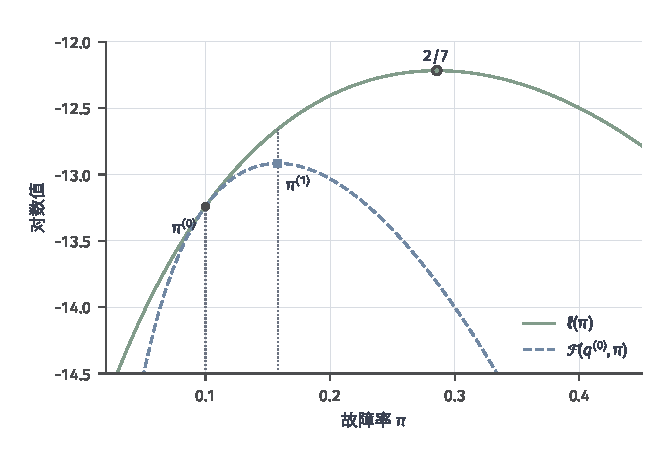
\includegraphics[width=105.412mm]{figures/06-probabilistic-graphical-models/03-learning/matplotlib/pgm-parameter-learning-em-bound/figure.pdf}
  \caption{故障率例子的第一轮EM。实线是观测对数似然，虚线是固定$\pi^{(0)}=0.1$后验所得的下界。两者在旧参数处相等；下界在$\pi^{(1)}\approx0.158044$处最大，而观测似然在$2/7$处最大。图中纵轴为自然对数，曲线可由正文公式直接复算。}
  \label{fig:pgm-parameter-learning-em-bound}
\end{figure}

\begin{figure}[htbp]
  \centering
  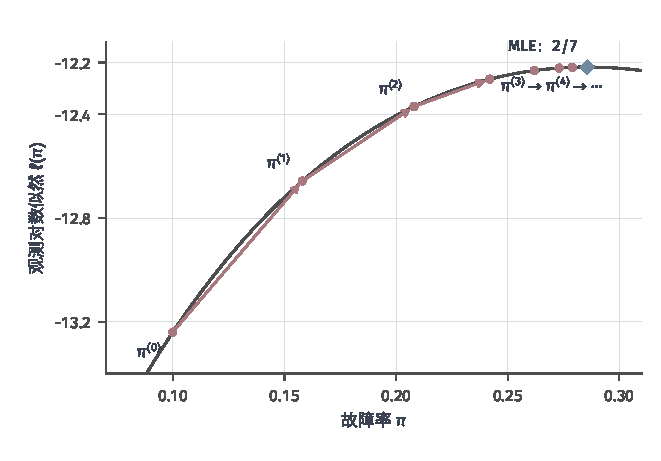
\includegraphics[width=105.412mm]{figures/06-probabilistic-graphical-models/03-learning/matplotlib/pgm-parameter-learning-em-trajectory/figure.pdf}
  \caption{同一标量例子的多轮EM轨迹。红点依次为$\pi^{(0)},\ldots,\pi^{(6)}$，纵坐标均使用观测对数似然而非各轮不同的下界；蓝色菱形是解析MLE $2/7$。该例的轨迹逐轮提高似然并接近解析最优点；一般模型中，单调性定理只保证相邻目标值不下降。}
  \label{fig:pgm-parameter-learning-em-trajectory}
\end{figure}

\subsection{广义EM与近似E步}
\label{sec:pgm-parameter-learning-em-extensions}

定理~\ref{thm:pgm-parameter-learning-em-monotonicity}的M步条件是保持或提高$Q$值。\term{广义EM}（generalized EM, GEM）保留精确E步，只要求M步改进同一个$Q$。例如，对$Q$做带回溯检查的梯度上升，或依次改进几个参数块，只要总更新不降低$Q$，就仍能保证观测似然不下降。步长与参数块更新因此需要检查$Q$的实际变化。

精确EM的E步要求算出真实后验；但在复杂模型里真实后验本身就无法精确求得（这正是第~\ref{chap:pgm-variational}章要处理的推断难题）。既然得不到精确后验，可以退而求其次：只在一个计算得起、又足够灵活的分布族$\mathcal{Q}$里找最接近真实后验的$q$，用它充当E步的结果。如果后验推断本身难以完成，则可以限制$q$属于某个可计算分布族$\mathcal{Q}$。\term{变分EM}（variational EM）在$\mathcal{F}(q,\bm{\theta})$上交替改进近似后验和参数：
\begin{equation}
  \begin{aligned}
    q^{(t+1)}
      &\in\argmax_{q\in\mathcal{Q}}\mathcal{F}(q,\bm{\theta}^{(t)}),\\
    \bm{\theta}^{(t+1)}
      &\in\argmax_{\bm{\theta}\in\Theta}
         \mathcal{F}(q^{(t+1)},\bm{\theta}).
  \end{aligned}
  \label{eq:pgm-parameter-learning-variational-em}
\end{equation}
精确最大化可以放宽为保证同一目标不下降的更新。在固定数据、模型和变分族下，两步都做到这一点，便有
\[
  \mathcal{F}(q^{(t+1)},\bm{\theta}^{(t+1)})
  \geq\mathcal{F}(q^{(t)},\bm{\theta}^{(t)}).
\]
受限后验通常留下非零KL间隙，因此旧点的下界与似然仍可能不同。两步改善给出的是ELBO单调性，观测似然的变化还取决于间隙如何变化\scite{pgm-parameter-learning-neal1998}

更明确地，记$K_t=\sum_j\operatorname{KL}(q_j^{(t)}\,\|\,p_{\bm{\theta}^{(t)}}(\bm{Z}_j\mid\bm{x}_j))$，并简记$\mathcal{F}_t=\mathcal{F}(q^{(t)},\bm{\theta}^{(t)})$，则式~\eqref{eq:pgm-parameter-learning-elbo-identity}给出
\[
  \ell(\bm{\theta}^{(t+1)})-\ell(\bm{\theta}^{(t)})
  =\mathcal{F}_{t+1}-\mathcal{F}_t+K_{t+1}-K_t.
\]
即使第一项非负，后验近似间隙的变化仍可能使总和为负。随机梯度或有噪声的下界估计，还可能连逐步ELBO单调性都不具备。Monte Carlo E步则用有限样本估计$Q$，其更新需控制采样误差，并核查实际改进。

MAP也可以采用EM式更新：E步仍计算给定当前参数的潜变量后验，M步改进$Q(\bm{\theta}\mid\bm{\theta}^{(t)})+\log p(\bm{\theta})$。在对应条件下，单调对象变成$\ell(\bm{\theta})+\log p(\bm{\theta})$，即相差常数的对数后验密度，而非数据似然本身。这个流程输出MAP参数点，完整参数后验的推断将在第~\ref{sec:pgm-parameter-learning-bayesian}节讨论。

\subsection{摊销推断与Wake--Sleep}
\label{sec:pgm-parameter-learning-amortized}

为每条记录、每一轮E步都单独解一个变分优化，在数据量大时代价很高，而且学到的“由观测推断后验”的能力无法在记录之间复用——处理过一万张相似图片后，来了新图片仍要从头优化。摊销推断换个思路：训练一个所有记录共享的映射（识别网络），让它直接吃进观测、吐出近似后验，把逐样本的优化“摊”成一次网络前向计算。变分EM若为每条记录分别保存$q_j$，新记录到来时还要重新求解一个局部优化问题。\term{摊销推断}（amortized inference）改用共享映射$q_{\bm{\phi}}(\bm{z}\mid\bm{x})$，由识别参数$\bm{\phi}$直接把观测映射为近似后验。对固定数据集，可以联合改进
\[
  \mathcal{F}(\bm{\theta},\bm{\phi})
  =\sum_{j=1}^n\mathbb{E}_{q_{\bm{\phi}}(\bm{Z}\mid\bm{x}_j)}
    [\log p_{\bm{\theta}}(\bm{x}_j,\bm{Z})
     -\log q_{\bm{\phi}}(\bm{Z}\mid\bm{x}_j)].
\]
共享映射减少逐样本优化与存储，近似质量可以按三个层次判断。若局部变分族$\mathcal{Q}$不包含真实后验，即使每条记录都求得族内最优$q_j^\star$，仍有由变分族限制带来的近似误差。再用共享映射$q_{\bm{\phi}}(\bm{z}\mid\bm{x})$代替这些逐样本最优解时，所选映射族的最佳结果与各$q_j^\star$之间的目标值差距才是\term{摊销误差}（amortization error），有限网络容量是其来源之一。实际训练若尚未达到该映射族内的最优$\bm{\phi}$，相对于该族最佳映射的剩余差距属于优化误差。具体的梯度估计与重参数化方法见第~\ref{sec:pgm-variational-amortized}节。

\term{Wake--Sleep算法}由Hinton等在1995年为随机Helmholtz机提出。它同时维护自上而下的\term{生成模型}（generative model）$p_{\bm{\theta}}(\bm{x},\bm{z})$与自下而上的\term{识别模型}（recognition model）$q_{\bm{\phi}}(\bm{z}\mid\bm{x})$，但两组参数不在同一个阶段更新。Wake阶段从训练数据取得$\bm{x}$，再由识别模型抽取$\bm{z}$，固定$\bm{\phi}$并更新生成参数$\bm{\theta}$，使这些“数据--解释”对在生成模型下更可能；Sleep阶段固定$\bm{\theta}$，从生成模型自上而下抽取$(\bm{x},\bm{z})$，再更新$\bm{\phi}$，使识别模型能够从生成出的$\bm{x}$恢复对应的$\bm{z}$\scite{pgm-parameter-learning-hinton1995}

这两个方向可以写成不同的总体目标。Wake阶段关于生成参数最大化
\begin{equation}
  J_{\mathrm{wake}}(\bm{\theta};\bm{\phi})
  =\frac{1}{n}\sum_{j=1}^n
    \mathbb{E}_{q_{\bm{\phi}}(\bm{Z}\mid\bm{x}_j)}
      [\log p_{\bm{\theta}}(\bm{x}_j,\bm{Z})],
  \label{eq:pgm-parameter-learning-wake-objective}
\end{equation}
它是固定识别模型后ELBO中依赖$\bm{\theta}$的部分，近似后验的间隙方向为$\operatorname{KL}(q_{\bm{\phi}}(\bm{Z}\mid\bm{x})\,\|\,p_{\bm{\theta}}(\bm{Z}\mid\bm{x}))$。经典算法用$q_{\bm{\phi}}$的样本形成局部随机更新，并不在Wake阶段沿识别参数求这个ELBO的梯度。

Sleep阶段关于识别参数最大化
\begin{equation}
  \begin{aligned}
    J_{\mathrm{sleep}}(\bm{\phi};\bm{\theta})
      &=\mathbb{E}_{p_{\bm{\theta}}(\bm{X},\bm{Z})}
          [\log q_{\bm{\phi}}(\bm{Z}\mid\bm{X})]\\
      &=-\mathbb{E}_{p_{\bm{\theta}}(\bm{X})}
          \operatorname{KL}\bigl(
            p_{\bm{\theta}}(\bm{Z}\mid\bm{X})
            \,\|\,q_{\bm{\phi}}(\bm{Z}\mid\bm{X})\bigr)+C(\bm{\theta}),
  \end{aligned}
  \label{eq:pgm-parameter-learning-sleep-objective}
\end{equation}
其中$C(\bm{\theta})$与$\bm{\phi}$无关。Sleep匹配生成后验到识别分布的KL，方向与Wake的ELBO间隙相反，外层输入又由当前生成模型加权。若生成模型低估真实数据的重要区域，Sleep样本便很少来自这些区域，相应识别映射也缺少训练。

Wake--Sleep的两个阶段因此对应不同目标与输入分布。Wake使用摊销后验更新生成参数，Sleep用生成数据训练识别参数；有限随机更新还包含抽样和求解误差。各阶段的实际目标可以改善，观测数据似然或真实数据ELBO的逐轮变化则需要另行分析，精确EM的单调性证明在这里缺少旧点贴合条件。

\section{观测缺失下的参数学习}
\label{sec:pgm-parameter-learning-incomplete}

除了模型主动引入的潜变量，现实数据还有另一类未观测：某些字段\emph{本应}记录、却因为设备损坏、患者失访、传感器漏报等原因没记下来。这两者都会让对应变量进入“要求和掉的未观测量”，所以边缘化与EM等工具可以复用；但缺失多了一个潜变量没有的问题——\emph{一个值为什么缺失}本身可能携带信息（如病情越重的患者越容易失访），忽略它会导致系统性偏差。观测缺失意味着按设计应记录的数据字段没有全部取得。缺失值与潜变量都形成未观测量，所以第~\ref{sec:pgm-parameter-learning-latent}节的边缘化和近似推断工具可以复用；记录过程若携带缺失值的信息，还要把这一信息纳入模型。本节据此确定如何把缺失字段接入已有推断与学习流程。

\subsection{缺失变量与缺失机制}
\label{sec:pgm-parameter-learning-missingness}

处理缺失数据前，需要先确定一个字段缺失的概率是否取决于它本应取的值。完全随机缺失可以安全忽略；若缺失概率随潜在数值变化，忽略缺失机制会带来偏差。因此要同时建模数据本身和记录状态。以$\bm{Y}$表示本应完整记录的数据向量，$R_i=1$表示$Y_i$已观测，$R_i=0$表示缺失。对一种固定模式$\bm{r}$，把$\bm{y}$拆为$\bm{y}_{\mathrm{obs}}$与$\bm{y}_{\mathrm{mis}}$，拆分位置由$\bm{r}$决定。数据模型为$p_{\bm{\theta}}(\bm{y})$，\term{缺失机制}（missingness mechanism）为$p_{\bm{\psi}}(\bm{r}\mid\bm{y})$，其中$\bm{\psi}$控制记录过程。这一条件分布描述记录概率如何依赖原始值，估计时需要关于采集过程的假设或信息。

可用漏记概率依赖哪些值来判断设备记录机制。设$F,A,S$均已记录，只有$H$可能缺失：独立日志故障对应MCAR，记录概率只依赖已知报警$A$对应MAR；在相同$F,A,S$下，$H$本身仍改变漏报概率时对应MNAR。图~\ref{fig:pgm-parameter-learning-missingness}以这些字段示意机制，具体类别由实际条件依赖决定。

\begin{figure}[htbp]
  \centering
  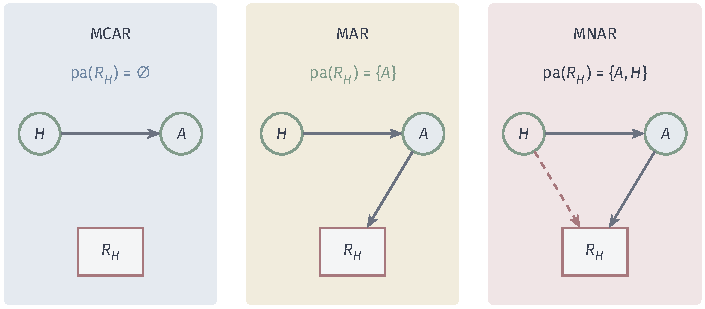
\includegraphics[width=112.000mm]{figures/06-probabilistic-graphical-models/03-learning/tikz/pgm-parameter-learning-missingness/figure.pdf}
  \caption{固定已观测的$F,S$后，温度记录指示量$R_H$的三种示意机制。三栏顶部直接给出$R_H$的父集，底部分别配独立日志故障、报警后安排检查、过热改变漏报概率的日常例子。$A$总是观测，$H$在$R_H=0$时不可见；右图表示给定已观测值后，记录概率仍随$H$变化的MNAR情形；若参数抵消该依赖，类别也随之改变。}
  \label{fig:pgm-parameter-learning-missingness}
\end{figure}

\subsection{可忽略性}
\label{sec:pgm-parameter-learning-ignorability}

MAR条件下，固定实际观测值后，记录概率与待积分的缺失值无关，因而可从积分中提出。对一条记录，观测似然分解为
\begin{equation}
  \begin{aligned}
    L(\bm{\theta},\bm{\psi})
      &=\int p_{\bm{\theta}}(\bm{y})
          p_{\bm{\psi}}(\bm{r}\mid\bm{y})
           \,\mathrm{d}\bm{y}_{\mathrm{mis}}\\
      &=p_{\bm{\psi}}(\bm{r}\mid\bm{y}_{\mathrm{obs}})
        p_{\bm{\theta}}(\bm{y}_{\mathrm{obs}}).
  \end{aligned}
  \label{eq:pgm-parameter-learning-ignorability-factorization}
\end{equation}
参数域可分离为$\Theta\times\Psi$时，关于$\bm\theta$的似然优化可省去机制因子。若还保留参数后验，先验分离$p(\bm\theta,\bm\psi)=p(\bm\theta)p(\bm\psi)$是一组充分条件：机制因子与其先验的积分有限且为正时，积分$\bm\psi$只留下与$\bm\theta$无关的常数。相关先验则可能使该积分仍依赖$\bm\theta$，此时后验需保留它。可忽略性简化的是参数计算，实际缺失字段仍在观测似然中被积分。下一小节据此接入每条记录的可见字段。

\subsection{可忽略缺失下复用未观测变量方法}
\label{sec:pgm-parameter-learning-ignorable-methods}

在可忽略条件下，可以把每条记录实际可见的部分作为$\bm{x}_j=\bm{y}_{j,\mathrm{obs}}$，把缺失部分作为$\bm{z}_j=\bm{y}_{j,\mathrm{mis}}$，直接复用第~\ref{sec:pgm-parameter-learning-latent}节的观测似然、梯度恒等式、精确EM或近似E步。模型若还含主动设置的潜变量$\bm{h}_j$，就把未观测量合并为$\bm{z}_j=(\bm{y}_{j,\mathrm{mis}},\bm{h}_j)$；不同记录可以有不同缺失模式，但每次推断都必须固定该记录实际观测到的分量。

这组记号将两类未观测量接入同一个积分工具，它们在数据获取上的含义仍不同。删除不完整记录会改变拟合所用的记录集合；单次均值或众数填补又省去了条件分布的变动。对离散模型，应计算相关家庭事件的后验期望计数；对高斯模型，还需二阶矩与交叉矩。若采用摊销推断，识别映射还需接收缺失掩码或等价的观测模式信息，以区分真正观测的值和用于输入格式的填充值。

\subsection{不可忽略缺失与可识别性}
\label{sec:pgm-parameter-learning-mnar}

MNAR时，记录过程在给定已观测值后仍依赖缺失值，式~\eqref{eq:pgm-parameter-learning-ignorability-factorization}通常不能分解。此时应为
\[
  p_{\bm{\theta},\bm{\psi}}(\bm{y},\bm{r})
  =p_{\bm{\theta}}(\bm{y})
   p_{\bm{\psi}}(\bm{r}\mid\bm{y})
\]
建立联合模型，把$\bm{R}$作为已观测变量，并对$\bm{Y}_{\mathrm{mis}}$以及原有潜变量共同边缘化。给定这个联合模型后，仍可使用第~\ref{sec:pgm-parameter-learning-latent}节的优化与推断工具；其中的完全数据模型包含采集过程，待估参数也包括$\bm{\psi}$。

联合模型的可识别性仍需检查。不同的数据分布与缺失机制可能诱导同一个$p(\bm{y}_{\mathrm{obs}},\bm{r})$，仅凭现有记录便无法区分它们。对未观测值怎样改变缺失概率的假设，需要由随访数据、外部测量、有效工具变量、受控采集设计或明确的参数约束提供额外信息；缺少这些信息时，可以对未识别的机制假设进行敏感性分析，报告它们对参数和预测的影响。EM负责给定联合模型后的求解，可识别性则由观测信息与模型限制共同决定。

\section{基于分布估计的参数学习}
\label{sec:pgm-parameter-learning-bayesian}

本节通过\term{分布估计}保留参数后验$p(\bm{\theta}\mid\mathcal{D})$，把未知参数本身作为推断变量。它与前面三种数据可见性设定交叉：无未观测变量且满足共轭条件时可能解析更新；含潜变量或缺失值时通常要联合近似参数与未观测变量；得到参数后验后，再通过后验预测把参数不确定性传给新数据。

\subsection{不含未观测变量的共轭后验}
\label{sec:pgm-parameter-learning-conjugacy}

前面的MLE/MAP只用到数据的充分统计量来找一个最优点。贝叶斯方法则要更新参数的整个分布，一个极为方便的情形是共轭：先验和似然属于同一个分布族，相乘后后验仍在该族内，于是学习退化为对少数几个“超参数”做加法更新（先验的虚拟计数 + 数据的真实计数）。不含未观测变量时，局部统计量不仅能用来找最优点，也能更新参数分布。\term{共轭先验}（conjugate prior）是与似然相乘后仍留在同一分布族中的先验，因此可通过更新有限组超参数表示整个后验。

对一个独立参数块$\bm{\eta}$，假设其似然中与参数有关的部分具有形式
\[
  p(\mathcal{D}_b\mid\bm{\eta})
  \propto\exp\{\bm{\eta}^\top\bm{S}_b-n_ba(\bm{\eta})\},
\]
其中$\bm{S}_b$是聚合充分统计量，$n_b$是该块的观测次数，$a$是对应对数归一化函数。若采用相对于指定参数测度、可归一化的先验$p(\bm{\eta}\mid\bm{\chi},\nu)\propto\exp\{\bm{\eta}^\top\bm{\chi}-\nu a(\bm{\eta})\}$，则
\begin{equation}
  p(\bm{\eta}\mid\mathcal{D}_b)
  \propto
  \exp\{\bm{\eta}^\top(\bm{\chi}+\bm{S}_b)
                 -(\nu+n_b)a(\bm{\eta})\}.
  \label{eq:pgm-parameter-learning-conjugate-update}
\end{equation}
指数相加给出$\bm{\chi}\leftarrow\bm{\chi}+\bm{S}_b$与$\nu\leftarrow\nu+n_b$。这一写法适用于拥有共同归一化函数的参数块，例如离散CPT的一行；一般条件指数族的归一化函数还依赖父节点值，需要按实际设计逐记录保留这些项。

在所有节点均已观测、没有参数共享且先验也按节点和CPT行独立分解时，似然的分解使后验同样局部分解：
\begin{equation}
  p(\bm{\theta}\mid\mathcal{D})
   =\prod_{i,a}
     \operatorname{Dirichlet}
       (\bm{\theta}_{i,a};
        \bm{\alpha}_{i,a}+\bm{N}_{i,a}).
  \label{eq:pgm-parameter-learning-local-posterior}
\end{equation}
数据沿图结构的作用在这里很具体：每条记录只给各节点家庭的相应单元格增加计数。父配置从未出现时，该行后验保持先验，反映这一局部条件尚未得到数据更新。对完整的线性高斯局部回归，适当的正态与逆Gamma联合先验也可以利用设计矩阵的交叉乘积解析更新，原理同样是聚合局部充分统计量\scite{pgm-murphy2012}

Dirichlet后验保留了整行概率的不确定性，而不只给出式~\eqref{eq:pgm-parameter-learning-cpt-map}的众数。记$\alpha_{i,a,0}=\sum_k\alpha_{i,a,k}$，则
\begin{equation}
  \mathbb{E}[\theta_{i,a,k}\mid\mathcal{D}]
    =\frac{N_{i,a,k}+\alpha_{i,a,k}}
            {N_{i,a}+\alpha_{i,a,0}}.
  \label{eq:pgm-parameter-learning-dirichlet-estimates}
\end{equation}
这个后验均值只需正超参数便定义良好，它将整个参数后验压缩成一个点，分布的宽度仍需其他摘要或完整后验来表达。均匀Dirichlet先验下，式~\eqref{eq:pgm-parameter-learning-cpt-map}的内部MAP与MLE相同，常见的加一平滑则来自本式的后验均值。

后验是否局部分解取决于似然和先验共同的结构。共享超参数会将原来独立的块联系起来，缺失数据的求和也通常打破式~\eqref{eq:pgm-parameter-learning-local-posterior}。EM的一轮期望计数依赖当前参数点，用于更新下一参数点。要保留参数不确定性，则需联合推断$p(\bm{\theta},\bm{z}_{1:n}\mid\mathcal{D})$；仅将该期望计数代入Dirichlet更新会得到一种额外近似。

设备例子也能展示后验保留了多少信息。表~\ref{tab:pgm-parameter-learning-device-counts}给出$5$次故障和$15$次正常，结合$\operatorname{Beta}(2,2)$先验得到$\pi\mid\mathcal{D}\sim\operatorname{Beta}(7,17)$。同一份数据的MLE、MAP与后验均值分别为$1/4$、$3/11$和$7/24$；前两者是不同目标的最优点，第三个数只是后验的一项摘要。该后验的方差为
\[
  \operatorname{Var}(\pi\mid\mathcal{D})
   =\frac{7\times17}{24^2\times25}
   =\frac{119}{14400}\approx0.008264.
\]
后验方差保留了故障率的剩余不确定性，$7/24$只概括其中心。新增完整记录时继续累加成功、失败计数即可，先验超参数则记录建模选择。

\subsection{含未观测变量的近似后验}
\label{sec:pgm-parameter-learning-approximate-posterior}

9.5.1的共轭更新之所以能解析完成，依赖“所有变量都观测、各参数块独立”这两个条件。一旦有潜变量或缺失值，参数后验就不再能与未观测量分开：看到数据后，“参数是多少”和“潜变量取什么”相互影响，必须联合推断，干净的计数加超参更新也随之失效。一旦含有潜变量或缺失值，参数后验通常要与未观测变量联合推断；非共轭局部模型和复杂参数共享还会进一步破坏解析形式。此时可以沿用第~\ref{chap:pgm-variational}章和第~\ref{chap:pgm-sampling}章的方法，其推断对象扩展为参数与状态的联合分布。以下用$\bm{z}_{1:n}$统称各条记录中的潜变量和实际缺失字段。对MNAR，$\mathcal{D}$还包含已观测的缺失指示，缺失机制参数$\bm{\psi}$也属于联合后验；为显式保留这一情形，下面的公式写出$\bm{\psi}$，不含缺失机制或机制可忽略时则删去所有$\bm{\psi}$项。

变分方法选取$q_{\bm{\phi}}(\bm{\theta},\bm{\psi},\bm{z}_{1:n})$，优化
\begin{equation}
  \begin{aligned}
    \mathcal{L}(\bm{\phi})
      &=\mathbb{E}_{q_{\bm{\phi}}}
       [\log p(\mathcal{D},\bm{z}_{1:n},\bm{\theta},\bm{\psi})
        -\log q_{\bm{\phi}}
          (\bm{\theta},\bm{\psi},\bm{z}_{1:n})],\\
    \log p(\mathcal{D})
      &=\mathcal{L}(\bm{\phi})
        +\operatorname{KL}\bigl(
          q_{\bm{\phi}}\,\|\,
          p(\bm{\theta},\bm{\psi},\bm{z}_{1:n}\mid\mathcal{D})
        \bigr).
  \end{aligned}
  \label{eq:pgm-parameter-learning-bayesian-elbo}
\end{equation}
这里数据参数$\bm{\theta}$与机制参数$\bm{\psi}$的先验都已进入联合分布，两者也都在证据中被积分；$\log p(\mathcal{D})$在模型和超参数固定时是常数。不含$\bm{\psi}$时，公式退化为只对数据参数与状态推断。此处优化近似分布参数$\bm{\phi}$，证据固定；变分EM则优化模型参数$\bm{\theta}$及状态近似，观测似然随$\bm{\theta}$变化。常用因子化假设可以降低计算量，却可能遗漏参数间相关性或后验的多个峰；下界求解的误差与分布族的表达误差需分别检查。

在共轭的变分更新中，期望计数确实可能作为超参数出现，但那属于特定变分族下的坐标更新。相应局部状态更新通常使用$\exp\{\mathbb{E}[\log\theta_{i,a,k}]\}$，而不是把后验均值代入$\theta$；一般有$\mathbb{E}[\log\theta]\ne\log\mathbb{E}[\theta]$。这些局部更新由各自目标导出，EM的点参数、贝叶斯变分的期望对数以及平滑计数对应不同计算。

MCMC则构造以参数后验或参数与潜变量联合后验为平稳分布的链，用其样本近似积分。若只关心普通可计算似然，后验中与参数无关的证据常数会在Metropolis--Hastings比率中约掉；无向模型的$Z(\bm{\theta})$却依赖候选参数，通常不会消失。这类模型可能仍需额外的内层推断或专门的采样构造。有限运行的积分精度还取决于混合、多峰之间的移动和查询相关的有效样本量，应结合相应诊断报告。

若后验在一个内部峰附近集中，还可以用\term{拉普拉斯近似}（Laplace approximation），即用峰值附近的二次曲率构造高斯分布。记$g(\bm{\theta})=\log p(\bm{\theta}\mid\mathcal{D})$，在局部MAP点$\widehat{\bm{\theta}}$作二阶展开；若$\bm{H}=-\nabla^2g(\widehat{\bm{\theta}})$正定，则
\[
  p(\bm{\theta}\mid\mathcal{D})
    \approx\mathcal{N}(\bm{\theta};
          \widehat{\bm{\theta}},\bm{H}^{-1}).
\]
边界峰、明显偏斜、多峰或不可识别方向会破坏这一局部高斯描述。对有约束的参数，宜先选择适当坐标，并将密度变换的Jacobian纳入目标，使曲率与MAP对应所用坐标的密度。比较这三类方法时，可以报告具体后验量或预测量的误差，以及相应计算预算。

\subsection{后验预测}
\label{sec:pgm-parameter-learning-posterior-predictive}

学出参数分布后做预测，要同时考虑两层不确定性：即使参数已知，新设备是否故障仍是随机的；而参数本身我们也不完全确定。后验预测把这两层一起积分掉，因此通常比直接代入单个参数估计的插件预测更保守、更能反映有限数据下的不确定性。得到参数后验后，新设备的状态仍具有随机性，而故障率本身也不完全确定。\term{后验预测}（posterior predictive）将这两种不确定性合并：在每个可能参数下计算新观测的分布，再按参数后验加权，
\begin{equation}
  p(\bm{x}_*\mid\mathcal{D})
   =\int p_{\bm{\theta}}(\bm{x}_*)
            p(\bm{\theta}\mid\mathcal{D})\,\mathrm{d}\bm{\theta}.
  \label{eq:pgm-parameter-learning-posterior-predictive}
\end{equation}
若预测还涉及新潜变量，应在内层同时消去它们。\term{插件预测}（plug-in prediction）则把某个点估计$\widehat{\bm{\theta}}$代入$p_{\bm{\theta}}(\bm{x}_*)$，计算较简单，但忽略了参数分布的宽度。

对单台设备的Bernoulli故障变量，后验预测恰好等于代入后验均值的结果：$p(F_*=1\mid\mathcal{D})=\mathbb{E}[\pi\mid\mathcal{D}]=7/24$。单设备故障概率对$\pi$线性，因此该查询仅需要一阶矩。其他查询还可能涉及更高阶矩。考虑两台在给定$\pi$后独立的新设备，则
\[
  \begin{aligned}
    p(F_{*,1}=1,F_{*,2}=1\mid\mathcal{D})
      &=\mathbb{E}[\pi^2\mid\mathcal{D}]
        =\frac{7\times8}{24\times25}
        =\frac{7}{75},\\
    p_{\mathrm{plug}}(F_{*,1}=1,F_{*,2}=1)
      &=(7/24)^2=\frac{49}{576}.
  \end{aligned}
\]
两者约为$0.09333$和$0.08507$，相差$\operatorname{Var}(\pi\mid\mathcal{D})$。积分共同参数后，两台设备不再后验预测独立：它们都受到同一故障率未知性的影响。对未来$m$台设备的故障数，完整预测服从Beta--二项分布，参数混合使其与固定平均故障率的二项分布不同。

条件预测还要说明新输入怎样被处理。纯条件模型把$\bm{x}_*$视为给定设计，使用$\int p_{\bm{\theta}}(\bm{y}_*\mid\bm{x}_*)p(\bm{\theta}\mid\mathcal{D})\,\mathrm{d}\bm{\theta}$。若训练的是联合生成模型，新输入本身也能提供参数信息，则严格的条件后验预测为
\[
  p(\bm{y}_*\mid\bm{x}_*,\mathcal{D})
  =\frac{\int p_{\bm{\theta}}(\bm{x}_*,\bm{y}_*)
                      p(\bm{\theta}\mid\mathcal{D})\,\mathrm{d}\bm{\theta}}
         {\int p_{\bm{\theta}}(\bm{x}_*)
                      p(\bm{\theta}\mid\mathcal{D})\,\mathrm{d}\bm{\theta}}.
\]
等价地，它用$p(\bm{\theta}\mid\mathcal{D},\bm{x}_*)$加权条件分布。只有在输入不更新相关参数等条件下，才能直接改用训练后的参数后验作权重。预测对象不同，所需的积分顺序与权重也可能不同。

\section{学习算法分析}
\label{sec:pgm-parameter-learning-analysis}

学出一组参数并不等于得到一个可靠模型：算法可能没把目标优化到位，模型族本身可能表达不了真实分布，即便两者都好，有限数据上学到的也未必适用于新记录。因此评价学习结果要分三个层次，它们对应三类不同来源、不能互相弥补的差距。学习结果可以从三个层次分析。表达能力考察固定图与局部分布族能否表示所需的观测分布，参数共享、潜变量和可识别性决定哪些差异可由模型表达并由数据区分。收敛性考察实际更新是否接近所选目标的最优候选、达到何种驻点，以及推断误差和计算规模如何影响求解速度。泛化性则考察从有限训练记录选择的候选能否预测新记录，重点是独立测试分布、参数不确定性和模型失配。以下在学习所需统计量、优化过程及结果评价中分别落实这三个问题。

\subsection{学习与推断的耦合}
\label{sec:pgm-parameter-learning-inference-coupling}

先从模型表达与学习所需的信息看各节的差异。固定图及局部分布族限定了候选分布：缺少必要的相互作用或使用不合适的局部族时，即使求解充分，也可能无法拟合目标观测分布。在这一族内，各种数据设定又提供不同统计量。观测完整且不含潜变量的有向图已经给出局部事件，独立参数块只需聚合计数或回归矩；联合无向图虽然观测完整，仍需计算全局归一化带来的模型期望；条件无向图需要对每个输入计算输出条件分布的期望；含潜变量或缺失值时，还要计算每条记录条件下的后验期望。若联合无向图同时含有潜变量，两类推断任务会同时存在。

例如，对充分统计量为$\bm{T}(\bm{x},\bm{z})$的无向指数族潜变量模型，平均观测似然梯度为
\begin{equation}
  \begin{aligned}
    \frac{1}{n}\nabla_{\bm{\theta}}\ell
      &=\frac{1}{n}\sum_{j=1}^n
        \mathbb{E}_{p_{\bm{\theta}}(\bm{Z}\mid\bm{x}_j)}
          [\bm{T}(\bm{x}_j,\bm{Z})]\\
      &\quad-\mathbb{E}_{p_{\bm{\theta}}(\bm{X},\bm{Z})}
          [\bm{T}(\bm{X},\bm{Z})].
  \end{aligned}
  \label{eq:pgm-parameter-learning-two-expectations}
\end{equation}
第一项问的是“这条观测记录可能来自哪些状态”，第二项问的是“模型不附加证据时会产生哪些状态”。第一项需要附加该记录证据的样本，第二项需要模型无证据的样本。两种期望共同进入参数梯度，因此后验易算的E步仍可能伴随配分函数难算的M步。

学习的内层推断成本随图结构变化。离散完整有向图可以一次扫描累加家庭计数，但表格存储量约为$\sum_i r_i\prod_{v\in\operatorname{pa}(i)}r_v$，高入度节点仍可能很贵。对最大状态数为$r$、诱导宽度为$w$的离散精确消元，主要因子运算规模通常含$r^{w+1}$；潜变量学习还要针对不同证据重复或批量复用这些运算。图固定时可以复用消元结构与消息调度，但参数更新后消息数值一般需要重算。相关算法见第~\ref{chap:pgm-elimination}章和第~\ref{chap:pgm-junction-tree}章。

\subsection{优化与可扩展性}
\label{sec:pgm-parameter-learning-scalability}

收敛速度的判断需要同时计算每轮成本与达到所需目标差距的轮数。样本数很大时，遍历全部记录可能成为每轮的主要成本。\term{随机梯度}（stochastic gradient）从小批量记录估计全数据梯度。若优化平均对数似然，大小为$b$的均匀小批量$\mathcal{B}$给出$b^{-1}\sum_{j\in\mathcal{B}}\nabla\log p_{\bm{\theta}}(\bm{x}_j)$；若优化总和目标，则相应乘以$n$。先验在总和目标中只出现一次；把整个目标除以$n$改成均值时，正则项也应同步除以$n$，以保持原有先验与数据的相对权重。

小批量降低经验项的每轮成本，内层推断仍决定更新的准确性。可把实际更新使用的梯度写成
\[
  \widehat{\bm{g}}^{(t)}
   =\nabla J(\bm{\theta}^{(t)})
      +\bm{b}_{\mathrm{inf}}^{(t)}
      +\bm{\xi}^{(t)},
\]
其中$\bm{b}_{\mathrm{inf}}^{(t)}$表示近似推断带来的系统偏差，$\bm{\xi}^{(t)}$表示中心化后的抽样波动。增加批量主要降低波动，固定步数链或受限变分族的系统偏差则需要改变内层求解来控制。偏差随参数变化时，更新可接近一个偏移后的平衡点，平滑训练曲线本身不足以识别原似然驻点。

参数共享减少自由度，同时限制候选分布；它也能汇集多个位置的数据以估计罕见配置。共享后，式~\eqref{eq:pgm-parameter-learning-dag-likelihood}虽仍是局部项之和，同一参数的梯度要从所有出现位置累加。同一大图上的模板实例通常相关，聚合它们时仍需保留模型内部依赖；独立设备或独立序列才提供相应的跨记录独立性。

\term{自动微分}（automatic differentiation）沿计算图应用链式法则，可同时处理共享参数与复杂局部网络；所得导数对应所写的计算目标。若反向传播穿过固定次数的消息更新，所得导数针对这个有限计算过程，与精确似然导数的差距需由推断近似分析。EM的M步则应固定E步分布，对$Q$中的新参数求导；梯度穿过旧后验构造时会多出另一组依赖项，形成不同更新。归一化项与后验期望的计算精度，仍决定上述导数与统计目标梯度的差距。

非凸点估计还依赖初始化。不同初值可能把EM、变分学习或一般梯度法送入不同的吸引区域，多次初始化可以比较这些区域内的目标值和预测表现，所得最好结果仍只在已探索区域内成立。潜变量未观测所留下的信息不足，还可能使参数与期望统计量调整缓慢，应结合目标变化与求解条件判断停止，而非仅看参数位移。

优化目标本身也可能没有有限最大值。高斯混合模型中，若一个$m$维分量保持固定正权重，把均值移到某个样本$\bm{x}_j$上，并令协方差为$\varepsilon^2\bm{I}$，该点密度正比于$\varepsilon^{-m}$。只要其他分量仍给其余样本正密度，令$\varepsilon\to0$就可使总似然无界。这种\term{退化解}（degenerate solution）来自目标的无界边界路径，沿该路径继续提高似然会缩小协方差，而无法到达有限参数最优点。对协方差加下界或采用适当先验可以排除相应路径，但这会改变原来的无约束MLE问题。

当训练集上的表现不理想时，盲目“再多迭代一会儿”未必有用，因为差距可能根本不来自优化没收敛。把误差按来源拆开，才能对症下药：数据不够、推断不准、优化不足需要完全不同的补救。收敛诊断还需区分目标误差来自何处。\term{统计误差}（statistical error）来自有限数据，即使精确求出样本目标的最优解，也未必接近总体最优参数；\term{推断误差}（inference error）来自近似边缘、期望或积分；\term{优化误差}（optimization error）则是相对于所选目标尚未充分求解的差距。模型族与真实分布的差异另产生表达或设定偏差。它们通常不在参数空间简单相加，但针对的计算不同：更多独立数据减少统计不确定性，改进内层推断控制近似偏差，继续优化减少当前目标的求解差距。

\subsection{学习结果的评价}
\label{sec:pgm-parameter-learning-evaluation}

预测新记录时，训练样本的数量与局部配置覆盖决定可用于估计的信息，图结构、参数共享和正则化则限制所选候选的自由度。罕见父配置可能只有少量记录，因而其参数仍有较大不确定性；共享或先验可借助其他信息，却也引入相应限制。训练和测试来自不同设备群体或采集机制时，还需检查这些限制及概率关系是否适用于新记录。以下评价分别检验参数解释、独立预测和模型失配。

解释参数时，先区分候选分布与其参数表示。若不同参数产生相同观测分布，就存在\term{不可识别性}（non-identifiability）；增加观测数量也只能确定该等价类。交换混合分量的编号并同时交换其权重与局部参数，观测分布不变，这称为\term{标签交换}（label switching）；因子模型的某些旋转、无向势函数的常数重分配以及MNAR模型中数据分布与缺失机制的抵消也会产生不唯一性。约束可以选定一个代表，外部信息可能恢复识别，这些选择的作用取决于所加信息。预测评价可优先报告可识别的量或重标记不变的结构，任意参数代表的机制解释则需要额外识别条件。

泛化性关注新记录，而训练似然描述整批训练数据的概率或密度。条件模型对应给定输入后的训练标签概率。MAP、ELBO或替代准则的改善具有各自目标含义，评价新记录时应另外计算所需的预测分数。要判断概率模型能否预测新记录，应使用未参与训练和调参的独立测试集；记录具有分组或时间依赖时，划分也应避免同一设备或未来信息泄漏到训练侧。测试平均预测对数似然可以写为
\[
  \frac{1}{n_{\mathrm{test}}}
  \sum_{j=1}^{n_{\mathrm{test}}}
    \log p_{\mathrm{pred}}(\bm{x}^{\mathrm{test}}_j).
\]
条件模型应改用对应的条件预测概率，缺失数据应使用实际观测部分的概率及所声明的缺失机制。比较分数时，应固定联合或条件查询以及连续变量的坐标和单位，使数值对应同一预测任务。

用ELBO评估时，所报告的量是预测对数似然的下界。不同模型或不同近似族的下界间隙可能不同，排名也可能受到影响。无向模型还需估计$Z$才能将能量转成概率；伪似然和CD指标也分别衡量其局部准则或有限步更新，归一化测试似然需要另行计算。报告应说明归一化、积分或采样近似所用的方法与误差来源。

对数似然衡量整份概率分配，还可以单独检查概率是否与实际频率吻合。\term{概率校准}（probability calibration）要求预测某事件概率约为$u$的记录中，该事件发生比例也约为$u$。对故障预测，可在独立记录上按预测概率分箱，比较每箱平均概率与故障频率，并同时报告箱内样本量或不确定性。箱内记录很少时，频率偏差可能来自抽样波动。恒定预测总体故障率也可校准，但缺少区分高风险与低风险的能力，因此还需结合区分能力和预测对数似然评价。

参数后验还支持更有针对性的模型检查。\term{后验预测检查}（posterior predictive check）从后验预测中生成与原数据设计相同的重复数据，再比较具有实际意义的统计量。例如，设备模型可以比较总报警率、各故障组的过热率，以及给定$H,S$后报警与故障之间是否仍有模型没有解释的关联。若研究对象包含缺失过程，复制数据时也应模拟相应记录机制，或明确固定了什么观测设计。观测统计量偏离后验预测的主要概率区域时，提示模型结构、局部分布或先验可能不适合当前数据。

后验预测检查定位已观察数据与模型的哪些统计特征不相容。它复用了拟合数据，所提供的是模型诊断；新数据上的泛化证据仍来自适当独立的预测评价。检查范围也取决于所选统计量，未被检查的结构可能仍有失配。积分参数得到的模型证据、比较两个证据之比的Bayes因子，以及BIC，主要服务于模型或结构比较，且需要考虑先验与正则条件。第~\ref{sec:pgm-structure-learning-scores}节将给出它们的定义，并说明这种比较与参数拟合、预测评价的区别。

\section{本章小结}
\label{sec:pgm-parameter-learning-summary}

本章从“模型给定”走向“从数据确定模型”，在图结构固定的前提下学习局部概率参数。贯穿全章的是开篇提出的两条正交主线。第一条是数据可见性：完整可见的有向模型可直接聚合计数或回归矩，是最容易的情形；无向模型因全局归一化，即使数据完整也要在学习内层反复计算模型期望；潜变量和缺失字段则进一步要求用后验期望（软计数）代替真实计数，使学习与推断深度耦合，而缺失字段还要额外考察记录机制是否携带信息。第二条是估计方式：MLE与MAP输出一个参数点，分布估计则保留整个参数后验，并通过后验预测把参数不确定性传入对新记录的预测。两条轴相互正交、可以组合。

算法结论应对应实际目标。精确EM用贴合下界推出观测似然不下降，GEM允许M步只改进同一$Q$；变分EM的两步改进对应ELBO，Monte Carlo E步还需控制抽样误差。Wake与Sleep分别更新不同分布下的目标，其变化需要按阶段解释。

表达能力由固定图、局部分布和参数约束限定；收敛性受目标形状、初始化、内层推断和计算规模影响；泛化性则需用新记录上的预测分数、校准及参数不确定性检验。模型诊断、求解诊断和独立预测评价提供不同证据，可识别性与退化边界决定这些结果能够如何解释。

\paragraph{扩展阅读}
Bishop的PRML第9章将完整数据估计、潜变量与EM联系起来；Koller与Friedman的教材补充图模型中的充分统计量和缺失机制。阅读时可将每种方法的观测似然、辅助目标及可识别条件逐项对应，理解目标改善如何转化为学习结论\scite{bishop2006,pgm-koller2009}

\chapter{结构学习}
\label{chap:pgm-structure-learning}

前一章把图的结构（哪些变量相连、边朝哪个方向）视为专家或设计给定的前提，只从数据估计局部条件分布的参数。实际数据往往没有提供可靠结构：只有设备运行记录时，故障、过热、报警和传感器之间的直接关系仍待确定。\emph{结构学习}研究如何根据数据和领域知识选择或评价这些连接。

结构学习比参数学习多了两类困难。第一，选择空间巨大且离散：参数学习在连续参数空间中优化，结构则要在$2^{\binom d2}$种边集中挑选，节点数稍多就不能逐一尝试。第二，观测数据通常只能把结构确定到一个等价类：若干箭头方向不同的图可以产生相同的观测分布，仅凭观测数据无法取舍。还要区分两个层次：连出一张能拟合数据、表示变量依赖的图，与把箭头解释成故障传播那样的因果方向并不相同；后者需要额外的机制假设或实验信息。

本章沿三类工具展开。\emph{条件独立检验}判断给定其他变量后两个变量是否仍相关，提供关于边是否存在的局部证据；\emph{评分}把整张图作为候选，用拟合程度与结构复杂度的平衡给出可比较的分数；\emph{搜索}根据这些证据在合法图空间中寻找高分候选。缺失观测和潜变量会改变可用证据。本章最后说明，仅有观测分布通常不足以把箭头解释为因果作用，还需要干预数据或额外的函数与噪声假设。

\section{结构学习的定义}
\label{sec:pgm-structure-learning-definition}

本节固定结构学习的对象、可能的输出形式和观测等价这一根本限制。记节点集合为$V=\{1,\ldots,d\}$，随机向量为$\bm{X}=(X_1,\ldots,X_d)^{\top}$，数据为$\mathcal{D}=\{\bm{x}_r:r=1,\ldots,n\}$，暂取样本独立同分布。给定候选图族$\mathfrak{G}$及各图对应的分布族$\mathcal{M}(\mathcal{G})$，\term{结构学习}（structure learning）利用数据和领域知识选择或评价依赖关系的图表示。候选范围可以规定边的类型，也可以限制父集大小、禁止特定边或仅允许树；缺失数据及多干预环境随后另行处理。

学习结果应表示数据能够确定的信息。用于预测时，可以选择拟合与复杂度折中的图；保留不确定性时，可以给出结构后验；高斯条件依赖可以用稀疏精度矩阵表示。若多张图在可用信息下无法区分，结果就应保留它们的共同关系。这些输出对应不同统计目标，并非把同一个确定结果换一种画法。

结构学习通常不能从纯观测数据中唯一恢复一张带确定箭头的图。有向图通过d-分离编码独立性；d-分离关系完全相同的不同有向无环图，即使箭头方向不同，也能表示同一批条件独立关系并拟合同一族分布，因此在观测数据下无法区分。具有相同d-分离关系的有向无环图组成\term{Markov等价类}（Markov equivalence class, MEC），“等价”指它们在纯观测数据下不可区分。两图等价要求两件事：一是忽略方向后相邻关系完全相同，即\term{骨架}（skeleton）相同；二是$i\to k\leftarrow j$且$i,j$本身不相邻的\term{无屏蔽碰撞结构}（unshielded collider，又称v-structure）也相同。碰撞结构是唯一能仅凭独立性模式判断方向的局部结构，对撞点处的条件化会打开路径。这里比较图所蕴含的全部独立关系，区别于特定参数取特殊值时靠数值抵消偶然产生的额外独立性；完整刻画见图模型教材\scite{pgm-koller2009}

局部条件分布没有额外函数形式限制时，等价图表示相同的分布族。例如$X_1\to X_2\to X_3$、$X_1\leftarrow X_2\leftarrow X_3$和$X_1\leftarrow X_2\to X_3$都只要求$X_1\perp X_3\mid X_2$。将两条边同时指向$X_2$则得到碰撞图，它要求两端边缘独立，属于另一个等价类。图~\ref{fig:pgm-structure-learning-equivalence}对照这些方向，展示三种表示共同确定的关系。

等价类包含多张图，逐一列出会造成冗余，也可能使某个代表图的方向被误认为由数据唯一确定。部分有向图只画出类内一致认同的方向：方向在类内可以翻转的边保留为无向边。\term{完成的部分有向无环图}（completed partially directed acyclic graph, CPDAG）把等价类共同确定的方向画成箭头、其余边画成无向边，也称观测本质图。未定向边的合法选择相互约束：补全必须保持无环且不增加无屏蔽碰撞。因此，“恢复CPDAG”表示恢复类内不变的关系；任取代表图所增加的方向仍属选择，而非新增数据证据。

\begin{figure}[!t]
  \centering
  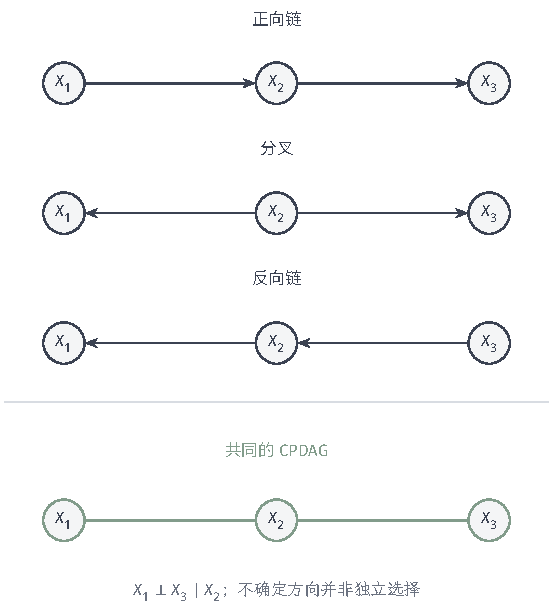
\includegraphics[width=93.652mm]{figures/06-probabilistic-graphical-models/03-learning/tikz/pgm-structure-learning-equivalence/figure.pdf}
  \caption{三种无碰撞有向图的等价表示。它们的骨架及条件独立关系相同，底部CPDAG保留这些共同信息；无向边表示类内方向可变。定向时两边须共同考虑：若都指向$X_2$，就会引入新碰撞，离开原等价类。}
  \label{fig:pgm-structure-learning-equivalence}
\end{figure}


候选空间决定结构搜索的计算规模。$d$个节点共有$2^{\binom d2}$种简单无向图；有向无环图即使固定一个拓扑序，也有这么多种边集可选，而拓扑序本身还有$d!$种排列。十几个节点时，候选图数量已经排除了暴力枚举，后续搜索算法需要在巨大空间中依据检验证据或评分作取舍。潜变量边缘化后的混合图允许不同端点标记，还受到整体合法性约束。扩大图族会增加可表示的分布，也增加参数、样本和搜索需求。频繁推断时，可把树宽等计算性质列为候选限制，并说明它们来自计算预算。

\section{有向图结构学习}
\label{sec:pgm-structure-learning-directed}

有向图结构学习使用两类性质不同的证据，再由搜索步骤组织比较。条件独立检验考察局部联系，似然及复杂度评分为整张图打分。搜索算法根据一种或两类证据寻找候选。检验和评分规定怎样比较结构，搜索规定怎样执行比较。检验是局部的：它一次只回答一对变量在给定某集合后是否独立；评分是整体的：它给每张候选图一个综合分数，同时考虑拟合与复杂度。

\subsection{条件独立约束}
\label{sec:pgm-structure-learning-constraints}

由条件独立检验删边依赖忠实性假设：数据中观察到的独立性应与图上的d-分离对应。即使两个变量在图上有边，具体条件概率参数也可能取特殊数值，使相关在数值上抵消而产生额外独立；这种独立来自参数巧合，不反映结构性质。\term{忠实性}（faithfulness）假设要求分布的条件独立与图上的d-分离一致，即独立只能来自图结构、不能来自参数抵消。若集合$S\subseteq V\setminus\{i,j\}$使$X_i$与$X_j$条件独立，在该假设下可删去$i,j$之间的边。总体分布未知时，算法实际检验的是
\[
  H_0:X_i\perp X_j\mid\bm{X}_S,
\]
并在未拒绝$H_0$时暂时删边。有限样本的检验功效会限制这一步：真实依赖过弱时也可能未被检出，因此未拒绝只是当前证据，尚未证明独立。

那么对离散数据，具体怎样检验“给定$\bm X_S$后$X_i$与$X_j$是否独立”？思路是比较两张计数表：一张是数据里实际观察到的$(X_i,X_j)$在各层$S$下的联合频率，另一张是假设两者独立时理应出现的频率（边缘频率相乘）。两者吻合则独立成立，差异越大越说明有直接依赖。离散记录可以按条件配置分层计数。令$N_{a,b,s}$统计$(X_i,X_j,\bm{X}_S)=(a,b,s)$的次数，点号表示对相应指标求和。比较联合频率与独立假设下的频率，得到似然比统计量
\begin{equation}
  G^2=2\sum_{a,b,s:N_{a,b,s}>0}
  N_{a,b,s}\log
  \frac{N_{a,b,s}N_{\cdot,\cdot,s}}
       {N_{a,\cdot,s}N_{\cdot,b,s}}.
  \label{eq:pgm-structure-learning-g-test}
\end{equation}
各单元概率为正、状态数固定且样本足够时，原假设下的统计量渐近服从卡方分布。若条件变量有$q_S$种配置，自由度为$q_S(r_i-1)(r_j-1)$，$r_i,r_j$是两端状态数。结构性零单元、稀有配置及小样本都可能破坏近似，检验校准需与这些条件一起检查。

上面的似然比检验还可以换一个更直观的信息论量来表达：它衡量“知道$X_j$以后，对$X_i$的不确定性平均能减少多少”。\term{条件互信息}（conditional mutual information）就是这个量，它比较条件联合分布与条件边缘乘积之间的差距；有限离散情形为
\[
  I(X_i;X_j\mid\bm{X}_S)
  =\sum_{a,b,s}p(a,b,s)
       \log\frac{p(a,b\mid s)}{p(a\mid s)p(b\mid s)}.
\]
正概率项构成各条件配置下KL散度的加权平均，故此量非负，且为零恰好表示条件独立。代入经验频率可得$\widehat I=G^2/(2n)$。$S$为空时，它成为\term{互信息}（mutual information），衡量边缘依赖；这种依赖可能通过其他变量传递，未必对应直接边。

联合高斯分布提供了另一个计算入口。分别将两端对$\bm{X}_S$作线性回归，残差的相关系数就是偏相关$\rho_{i,j\mid S}$；在非退化高斯设定中，它为零等价于条件独立。对样本偏相关$\widehat\rho$作Fisher变换，得到
\[
  Z=\frac{\sqrt{n-|S|-3}}{2}
    \log\frac{1+\widehat\rho_{i,j\mid S}}
                  {1-\widehat\rho_{i,j\mid S}},
\]
在原假设$\rho_{i,j\mid S}=0$下，取$n>|S|+3$且相应渐近近似适用时，$Z$近似服从标准正态分布。非高斯数据中的零偏相关只排除某类线性关系，需要更丰富的统计信息才能检验条件独立。核检验可用于非线性关系，其结论仍依赖核、正则化及零分布校准；一般回归残差不相关也不足以替代原变量条件独立。

下面用同一张计数表比较检验、评分和搜索。取三个二值测量量$X_1,X_2,X_3$，可以把它们理解为设备的状态指示，数值则重新构造。表~\ref{tab:pgm-structure-learning-counts}含100条教学记录，各变量的$0$和$1$均出现50次，未使用真实测量数据或前章故障模型参数。

\begin{table}[htbp]
  \centering
  \begin{tabular}{ccc r@{\qquad}ccc r}
    \toprule
    $x_1$ & $x_2$ & $x_3$ & 次数 & $x_1$ & $x_2$ & $x_3$ & 次数 \\
    \midrule
    0 & 0 & 0 & 36 & 1 & 0 & 0 & 4 \\
    0 & 0 & 1 & 9  & 1 & 0 & 1 & 1 \\
    0 & 1 & 0 & 1  & 1 & 1 & 0 & 9 \\
    0 & 1 & 1 & 4  & 1 & 1 & 1 & 36 \\
    \bottomrule
  \end{tabular}
  \caption{100条人工二值记录。一种生成表示是：从公平根变量出发，沿两条边分别以$0.1$、$0.2$的概率独立翻转。该表示恰好产生表中频率；其他观测等价方向也可产生同一分布，因果方向因而尚未确定。}
  \label{tab:pgm-structure-learning-counts}
\end{table}

记经验频率为$\widehat p$。两端的联合频率$\widehat p(X_1=1,X_3=1)=0.37$，超过边缘乘积$0.25$，显示边缘依赖。固定$X_2=0$后，一格条件频率却可写成
\[
  \widehat p(X_1=0,X_3=0\mid X_2=0)
  =\frac{36}{50}=\frac{45}{50}\frac{40}{50}.
\]
其余三格以及$X_2=1$层也满足乘积分解，因此经验条件互信息和$G^2$均为零（见式~\eqref{eq:pgm-structure-learning-g-test}）。这些精确等式来自构造；从条件独立总体随机抽样时，经验表一般仍有波动。

有了检验方法，还存在一个算法组织问题：若对每一对变量都尝试其余$d-2$个变量的所有子集作为条件集，子集数目随节点数指数增长，很快无法负担。PC算法的关键技巧是“边一旦因独立而删除，就不必再考虑”，因此只需在两个端点\emph{当前还保留的邻居}里寻找能让它们独立的条件集，并且条件集从最小（空集）开始、逐步增大；稀疏图里每个节点的邻居很少，这大幅压缩了检验次数。\term{PC算法}（PC algorithm）正是用这样逐渐扩大的条件集组织这些检验。它从完全无向图出发，按$|S|=0,1,\ldots$处理相邻点对$i,j$，在$i$的当前邻居中去掉$j$后选$S$，并考察交换两端后的候选。未拒绝独立时删边，记录分离集$\operatorname{Sep}(i,j)$；各相邻点对均无足够大的候选集时，骨架搜索停止。在忠实性及准确独立判定下，邻域中的候选足以找到必要分离集，可省去全节点子集枚举。

骨架只回答了“谁和谁相连”，箭头方向又从哪里来？唯一能仅凭独立性辨认出的方向就是碰撞结构：若$i,j$在给定不含$k$的某集合时独立、而一旦条件化到$k$反而变得相关（等价地说，$k$不在$i,j$的分离集中），那么$k$必定是对撞点，可定为$i\to k\leftarrow j$。定出这些碰撞后，其余方向并不是自由的，而要靠“不能制造新的碰撞”和“不能形成有向环”这两条硬约束逐条传播推出——能唯一确定的才画箭头，剩下的留作无向。骨架随后决定哪些三元组可以定向。对无屏蔽的$i-k-j$，若$k\notin\operatorname{Sep}(i,j)$，就置为$i\to k\leftarrow j$，再反复应用保持等价类的定向规则。例如$i\to k-j$且$i,j$不相邻时，需定为$k\to j$以避免新碰撞；已有$i$到$j$的有向路径时，需排除$j\to i$以避免环。完整算法使用完整规则集，以上两条只说明其作用。总体独立信息正确时可得到CPDAG；高维高斯一致性还要求稀疏性及非零偏相关有足够强度\scite{pgm-structure-learning-kalisch2007}

同一计数表的三对边缘关系给出以下统计量：
\[
  \begin{aligned}
    G^2_{1,2}&\approx73.6128,\\
    G^2_{2,3}&\approx38.5490,\\
    G^2_{1,3}&\approx24.0181.
  \end{aligned}
\]
用显著性水平$0.05$的渐近检验演示，它们均超过自由度1的临界值$3.841$。给定$X_2$后，$1,3$的统计量为零，故删去$1-3$并记录$\operatorname{Sep}(1,3)=\{2\}$。骨架成为$1-2-3$，三个方向仍无法由这组证据区分（见图~\ref{fig:pgm-structure-learning-equivalence}）。条件表中有稀有格，这里只演示操作，卡方近似的小样本准确性需另外检验。

局部误判还会传递到后续步骤。若把$1,3$误判为边缘独立，空分离集可能导致错误碰撞定向；误删边又会缩小后面的候选邻域。有限样本实现因此需要处理检验冲突、记录节点顺序，或采用稳定化邻接更新，使这些选择能够复核。

\subsection{结构评分与后验}
\label{sec:pgm-structure-learning-scores}

逐条做独立检验有两个固有弱点：一是大量检验之间会累积错误、还可能给出相互冲突的结论；二是它只能回答“这条边在不在”，无法直接比较两张都“大致合理”的图谁更好，也没有内建的复杂度控制。另一条路线把每张图看成一个完整模型，用一个标量分数统一衡量“它对数据拟合得多好”以及“它有多简单”，从而可以直接在候选图之间排序。检验逐个考察独立关系，评分则汇总整张图对数据的拟合。先取观测完整、无潜变量的离散模型：$X_i$有$r_i$个状态，父集有$q_i$种配置。令$N_{i,j,k}$统计节点状态$k$与父配置$j$的共同次数，$N_{i,j}=\sum_kN_{i,j,k}$。各条件表自由变化时，最大似然的对数得分为
\begin{equation}
  \ell(\widehat{\bm{\theta}}_{\mathcal{G}};\mathcal{D})
  =\sum_{i=1}^{d}\sum_{j=1}^{q_i}\sum_{k=1}^{r_i}
    N_{i,j,k}\log\frac{N_{i,j,k}}{N_{i,j}}.
  \label{eq:pgm-structure-learning-local-likelihood}
\end{equation}
零频项按$0\log0=0$解释；整行没有记录时，数据未规定该行条件分布，需要另选归一化概率，跳过$0/0$计算。对数得分按节点分解，修改某个父集只改变对应局部项。

为什么不能直接选似然最大的图？因为加边只会给模型增加自由参数、扩大它能表示的分布范围，却从不会让最优拟合变差——大模型总能把新增边的参数设成“该依赖不起作用”而退化成小模型。于是越稠密的图在训练数据上似然越高，纯粹最大化似然必然选出一张近乎全连接的图，把数据里的随机噪声也当成结构，这就是过拟合。要得到能泛化的结构，必须在“拟合更好”和“参数更多”之间加一道惩罚。\term{贝叶斯信息准则}（Bayesian information criterion, BIC）从似然中扣除参数代价；本章用越大越好的得分形式：
\begin{equation}
  \begin{aligned}
    \operatorname{Score}_{\mathrm{BIC}}(\mathcal{G})
      &=\ell(\widehat{\bm{\theta}}_{\mathcal{G}};\mathcal{D})
        -\frac{k_{\mathcal{G}}}{2}\log n,\\
    k_{\mathcal{G}}&=\sum_iq_i(r_i-1).
  \end{aligned}
  \label{eq:pgm-structure-learning-bic}
\end{equation}
此处$k_{\mathcal{G}}$统计自由参数，而非边数。将得分乘$-2$后最小化，得到软件中常见的等价排序。把BIC解释为对数边缘似然的渐近近似，还需固定维数、内点参数和非奇异信息矩阵等正则条件，潜变量模型的奇异性可能使该解释失效。

复杂度惩罚还可以从信息编码的角度重新理解：一个好模型应当让“先描述模型本身、再借助模型描述数据”这两段编码的总长度尽量短——复杂模型自身要花更多比特去描述，但通常能让数据部分编码得更短，二者权衡的最优点正是“恰到好处的结构”。这就是最小描述长度的思想。\term{最小描述长度}（minimum description length, MDL）同时计算描述模型和在给定模型后编码整份数据所需的信息。某些近似与BIC有相同主导惩罚，具体编码还可包含图结构本身。选择准则时应规定参数化、复杂度及得分方向，再用它们比较候选。

在教学表中，独立模型有3个参数，无碰撞链有5个，完整三节点有向无环图有7个。自然对数似然分别为$-207.9442$、$-151.8633$、$-151.8633$：完整图的额外表示能力没有在这张表中增加拟合。BIC分别为$-214.8519$、$-163.3762$、$-167.9814$，因而选择链的复杂度。三种观测等价链仍获相同支持，评分尚未确定因果方向。

BIC用一个渐近的惩罚项近似地控制复杂度；贝叶斯观点下有一个更自然的“自动惩罚”机制：不要只取模型拟合最好的那一组参数，而是把该图下\emph{所有}可能参数的似然按先验平均起来。参数越多、先验铺得越开的复杂模型，其概率质量被摊得越薄，平均后反而不占优，从而天然抑制过拟合。参数积分提供另一种比较方式。\term{边缘似然}（marginal likelihood）将数据似然在参数先验下平均，以此衡量一张图整体支持数据的程度。结合结构先验，得到
\begin{equation}
  \begin{aligned}
    p(\mathcal{D}\mid\mathcal{G})
      &=\int p(\mathcal{D}\mid\bm{\theta},\mathcal{G})
              p(\bm{\theta}\mid\mathcal{G})\,\mathrm{d}\bm{\theta},\\
    p(\mathcal{G}\mid\mathcal{D})
      &\propto p(\mathcal{D}\mid\mathcal{G})p(\mathcal{G}).
  \end{aligned}
  \label{eq:pgm-structure-learning-posterior}
\end{equation}
积分既考虑最佳拟合，也考虑先验支持中有多大区域能够拟合数据。只在极窄区域取得高似然的结构，未必有高边缘似然；复杂度控制在这里与参数先验共同发生作用。

两张图的数据支持可以用边缘似然之比比较，这就是\term{Bayes因子}（Bayes factor）。设各模型参数先验已归一化，两个证据有限，且第二个证据严格为正，则
\begin{equation}
  \begin{aligned}
    \operatorname{BF}_{12}
      &=\frac{p(\mathcal{D}\mid\mathcal{G}_1)}
              {p(\mathcal{D}\mid\mathcal{G}_2)},\\
    \frac{p(\mathcal{G}_1\mid\mathcal{D})}
         {p(\mathcal{G}_2\mid\mathcal{D})}
      &=\operatorname{BF}_{12}
        \frac{p(\mathcal{G}_1)}{p(\mathcal{G}_2)}.
  \end{aligned}
  \label{eq:pgm-structure-learning-bayes-factor}
\end{equation}
第二式还需$p(\mathcal{G}_2)>0$，并要求全体候选的总数据证据有限而为正。后验赔率等于Bayes因子乘结构先验赔率。Bayes因子含模型内参数先验的作用，结构先验赔率体现外层图先验的作用。若Bayes因子为$3$、结构先验赔率为$1/2$，后验赔率便为$3/2$。

观测完整、无潜变量的离散模型中，独立的Dirichlet先验允许精确积分。对各条件表行取$\bm{\theta}_{i,j}\sim\operatorname{Dirichlet}(\alpha_{i,j,1},\ldots,\alpha_{i,j,r_i})$，其中$\alpha_{i,j,k}>0$、$\alpha_{i,j}=\sum_k\alpha_{i,j,k}$。乘上该行似然后，参数指数由$\alpha_{i,j,k}-1$变成$\alpha_{i,j,k}+N_{i,j,k}-1$，积分就化为更新前后的归一化常数之比。全部行相乘为
\begin{equation}
  p(\mathcal{D}\mid\mathcal{G})
  =\prod_{i,j}
    \frac{\Gamma(\alpha_{i,j})}
         {\Gamma(\alpha_{i,j}+N_{i,j})}
    \prod_k
    \frac{\Gamma(\alpha_{i,j,k}+N_{i,j,k})}
         {\Gamma(\alpha_{i,j,k})}.
  \label{eq:pgm-structure-learning-dirichlet}
\end{equation}
$\mathcal{D}$按逐条记录定义，所以这里无需再加依结构而变的多项式计数系数。不同的Dirichlet超参数都能构成贝叶斯狄利克雷评分；若还希望等价图得分相同，超参数之间需满足进一步协调条件。

\term{贝叶斯狄利克雷等价评分}（Bayesian Dirichlet equivalent score, BDe）通过协调先验，使等价图获得相同边缘似然。一种构造先给严格为正的联合先验分布$p_0$及共同\term{等效样本量}（equivalent sample size）$\alpha>0$，再按候选父集的边缘设置伪计数：
\[
  \alpha_{i,j,k}
  =\alpha\,p_0(X_i=k,\bm{X}_{\operatorname{pa}(i)}=j).
\]
$j,k$是相应配置的编号，全部伪计数由同一个联合分布导出。结合参数独立性、参数模块性及似然等价性假设，等价图的积分值相同。若图先验在类内不同，后验仍会区分这些图，这种差异应归于先验贡献\scite{pgm-structure-learning-heckerman1995}

\term{均匀BDe评分}（BDe uniform, BDeu）选择均匀$p_0$，使每格$\alpha_{i,j,k}=\alpha/(q_i r_i)$、每行总量为$\alpha/q_i$。这里均匀的是用于分配伪计数的联合分布$p_0$，图结构先验另行选择。以二值$X_2$有一个二值父节点、$\alpha=4$为例，每格伪计数为1；父状态$X_1=0$有$(45,5)$次记录，后验均值变为$(46/52,6/52)$，最大似然则为$(0.9,0.1)$。增加父节点会把共同总量分散到更多配置，稀疏记录中$\alpha$可能改变图的排序，需比较其敏感性。

取同一$\alpha=4$并代入式~\eqref{eq:pgm-structure-learning-dirichlet}，正向链、分叉和反向链的对数边缘似然均约为$-161.968668$。三图共享数据证据，这个可复算结果也展示了BDeu的评分等价性。

当好几张图的后验概率都不可忽略时，硬选其中一张会丢掉这种结构层面的不确定性，而且预测可能对“碰巧选了哪张”过于敏感。更稳健的做法是不做单一选择，而是让每张图都按其后验概率对预测投票。\term{贝叶斯模型平均}（Bayesian model averaging, BMA）正是以结构后验为权重汇总预测分布：
\[
  p(\bm{x}_{\mathrm{new}}\mid\mathcal{D})
  =\sum_{\mathcal{G}\in\mathfrak{G}}
    p(\bm{x}_{\mathrm{new}}\mid\mathcal{D},\mathcal{G})
    p(\mathcal{G}\mid\mathcal{D}).
\]
各图内的预测继续积分参数后验；边是否存在等特征也可用相应指示函数加权。结构采样或高分候选集合只能近似这一平均，需说明覆盖范围。重复搜索得到同一图衡量的是搜索行为，其频率尚非结构后验。按等价类平均时，还要规定先验作用于图还是类，以处理各类代表图数目不同的影响。

\subsection{结构空间搜索}
\label{sec:pgm-structure-learning-search}

评分解决了“如何比较两张图”，却没有解决“如何在指数级多的合法图里找到高分的那张”。最常用的实用策略是贪心局部搜索：从一张满足无环等约束的图出发，每一步只考虑对当前图做一次小改动（加一条边、删一条边、反转一条边），在所有合法且能提高分数的改动里选收益最大的一个执行，直到任何局部改动都不再涨分为止。这样做通常很快，但只保证停在“邻域内最好”的局部最优，不保证全局最优。评分给定后，搜索仍要找到合法的高分图。局部方法从满足约束的图出发，检查加边、删边、反向的候选，验证无环和领域限制，再选得分增益最大的正增益操作。没有合法改进时停止，只保证当前邻域局部最优。加边更新一个局部得分，反向更新两端；父集缓存省去重复拟合，无环检查仍需整体进行。重启、禁忌或扩大邻域可探索更多候选，全局最优另需证明或认证。

一次移动的收益还可分解为拟合与复杂度两项。向$X_i$的父集$P$加入$X_j$时，以$\widehat I$表示经验条件互信息，离散BIC增益为
\begin{equation}
  \Delta\operatorname{Score}_{\mathrm{BIC}}
  =n\widehat I(X_i;X_j\mid\bm{X}_P)
   -\frac{\Delta k}{2}\log n.
  \label{eq:pgm-structure-learning-score-gain}
\end{equation}
新增条件变量减少的经验条件熵带来第一项，额外自由参数带来第二项。空图加入$1\to2$时，$\widehat I=0.368064$、$\Delta k=1$，增益为$36.8064-2.3026=34.5038$。这里互信息服务于惩罚评分，接受移动由增益决定，区别于固定显著性水平的独立检验。

前面的爬山搜索把每一张有向无环图当作独立状态，于是同一等价类里若干得分完全相同的代表图会被反复考察、来回摆动，浪费大量步数。一个更聪明的状态空间是直接把整个等价类（用CPDAG表示）当作一个状态来搜索，避免在数据根本无法区分的图之间空转。\term{贪心等价搜索}（greedy equivalence search, GES）因此直接以CPDAG为状态，先前向插入、再后向删除，各阶段在没有合法正增益时停止。一次移动可能同时规定多个端点，再补全为新CPDAG，需要满足等价类操作的合法性。在固定节点数、样本量趋于无穷的条件下，GES可恢复真实分布的Markov等价类。该保证还依赖评分等价、可分解和局部一致性，以及真实分布具有候选有向图的完美映射等条件。局部一致性要求评分在大样本下奖励补上遗漏依赖、惩罚加入多余依赖\scite{pgm-structure-learning-chickering2002}

节点数较小时，可以枚举子问题求精确最优。对可分解评分，记$s_i(P)$为节点$i$采用父集$P$的得分，$F(U)$为节点子集$U$上的最佳有向无环图得分。非空有向无环图总有无出边的汇点，故可以按最后节点递推：
\begin{equation}
  \begin{aligned}
    F(\varnothing)&=0,\\
    F(U)&=\max_{i\in U}\left\{
      F(U\setminus\{i\})
      +\max_{P\subseteq U\setminus\{i\}}s_i(P)\right\}.
  \end{aligned}
  \label{eq:pgm-structure-learning-dp}
\end{equation}
递推把$i$置于拓扑序末尾，先优化剩余图，再选择$i$在剩余节点中的父集。枚举汇点便覆盖全部有向无环图。即使预计算了最佳父集，子集数仍随节点数指数增长，精确解需要相应时间与内存。

还可将父集选择交给整数规划。每个候选$P$对应二值变量$z_{i,P}$，目标为$\sum_{i,P}s_i(P)z_{i,P}$，约束$\sum_Pz_{i,P}=1$保证每个节点选一个父集。为排除环，还需对每个非空$U\subseteq V$要求
\[
  \sum_{i\in U}\ \sum_{P:P\cap U=\varnothing}z_{i,P}\geq1.
\]
这个约束要求每个诱导子图至少有一个内部无父节点的点。有向无环图满足它，环上的节点集合则违反它。约束本身有指数多个，求解器可按需加入违反项；完成最优性认证后，才得到已声明父集空间内的最优解。预先删去的父集仍限制该认证的范围。

贪心搜索是在离散的图空间里一步步挪动。另一类思路是把“有没有边”编码成一个连续矩阵里的数值，从而把结构选择变成可以用梯度求解的连续优化问题；难点在于必须用一条连续可微的约束来表达“图中不能有环”这个离散要求，NOTEARS正是通过矩阵指数给出了这样一条约束。搜索也可改用连续的边权表示。令$\bm{W}\in\mathbb{R}^{d\times d}$的非零元素$W_{i,j}$表示$i\to j$，中心化样本按行排成$\bm{Y}\in\mathbb{R}^{n\times d}$。NOTEARS以线性残差衡量拟合，以$\lambda\geq0$的稀疏惩罚控制边权，并将无环性写为等式约束：
\begin{equation}
  \begin{aligned}
    \min_{\bm{W}}\quad&
      \frac{1}{2n}\lVert\bm{Y}-\bm{Y}\bm{W}\rVert_{\mathrm F}^{2}
      +\lambda\lVert\bm{W}\rVert_1,\\
    \text{满足}\quad&
      h(\bm{W})=
      \operatorname{tr}\!\left(\exp(\bm{W}\circ\bm{W})\right)-d=0.
  \end{aligned}
  \label{eq:pgm-structure-learning-notears}
\end{equation}
$\circ$表示逐元素相乘，$\exp$表示矩阵指数，$\lVert\bm{W}\rVert_1$是全部元素绝对值之和。为看清约束为何排除环，令$\bm{B}=\bm{W}\circ\bm{W}$并展开矩阵指数：
\[
  h(\bm{W})=\sum_{m=1}^{\infty}
     \frac{\operatorname{tr}(\bm{B}^m)}{m!}.
\]
非负矩阵$\bm{B}$的$\operatorname{tr}(\bm{B}^m)$累加长度$m$的闭合有向游走权重。存在有向环时至少一项为正；无环时所有项均为零。因此$h(\bm{W})=0$恰好要求支撑图无环，自环也被排除。其梯度$2\bm{W}\circ[\exp(\bm{W}\circ\bm{W})]^{\top}$可用于增广拉格朗日等数值求解\scite{pgm-structure-learning-zheng2018}

平滑约束方便求导，但无环可行集合仍非凸，数值算法需要另外分析最优性。有限容差给出的$h$近零值还应配合最终图的拓扑检查。平方残差的统计解释依赖线性模型、变量尺度和噪声假设；无环等式只控制结构合法性，尚未决定方向的因果含义。

检验与评分还可以分阶段配合。先用条件独立证据筛选邻接或父集，再在缩小空间内优化BIC、BDe等评分，能降低搜索量；筛选漏掉的真边也因此失去后续竞争机会。PC式筛选、BIC评分和有向图爬山分别规定了筛选、比较及搜索，可以组成同一流程。

\subsection{观测缺失与结构EM}
\label{sec:pgm-structure-learning-structural-em}

上面的评分公式都建立在“每条记录的家庭计数拿得到”之上。一旦有变量缺失，某个节点的父配置计数就凑不齐，而评分之所以能按节点分解、能局部增删边，靠的正是这些计数；于是缺失数据同时破坏了“算分”和“搜索”的便利。更麻烦的是，现在连图结构本身都在变动，缺失值该按哪张图的结构去推断也随之变化。自然的办法是把第9章的EM与结构搜索结合起来：在当前图下用后验分布“软补”缺失值、得到期望计数，再据此给候选图评分并允许改动父集。若部分记录缺少$X_2$，家庭计数$N_{i,j,k}$便无法直接取得。每条记录需先边缘化未测变量，观测似然因此失去简单的节点分解。下文取可忽略的缺失机制，例如随机缺失且机制参数与模型参数可区分；直接删除不完整记录可能改变分布，缺失依赖未观测值时则通常要把缺失指示也纳入模型。

\term{结构期望最大化}（structural expectation maximization，结构EM）用当前图推断缺失量，再据此比较新的图。它扩展了固定图EM的M步，允许更新父集。取有限离散未观测量$\bm{Z}$、观测记录$\mathcal{D}_{\mathrm{obs}}$，第$t$轮的当前后验为
\[
  q^{(t)}(\bm{Z})
  =p(\bm{Z}\mid\mathcal{D}_{\mathrm{obs}},
                  \mathcal{G}^{(t)},\bm{\theta}^{(t)}).
\]
为了给候选图评分，需要它各节点家庭的期望计数：
\[
  \overline N_{i,j,k}^{(t)}
  =\sum_{r=1}^{n}
    \mathbb{E}_{q^{(t)}}\!
      \left[\mathbf{1}\{X_{r,i}=k,
        \bm{X}_{r,\operatorname{pa}_{\mathcal{G}}(i)}=j\}\right].
\]
$X_{r,i}$指记录$r$中的节点$i$，已测分量在期望中固定。父集随候选图而变，所需联合后验作用域也会改变；E步因此须覆盖候选家庭，不能只计算当前边对应的边缘。

比较不同图的前提是它们使用同一未观测变量空间。对惩罚似然，固定当前后验并构造
\begin{equation}
  \begin{aligned}
    Q^{(t)}(\mathcal{G},\bm{\theta})
      &=\mathbb{E}_{q^{(t)}}[
          \log p(\mathcal{D}_{\mathrm{obs}},\bm{Z}
                     \mid\mathcal{G},\bm{\theta})],\\
    \mathcal{F}^{(t)}(\mathcal{G},\bm{\theta})
      &=Q^{(t)}(\mathcal{G},\bm{\theta})+H(q^{(t)})
        -\operatorname{pen}(\mathcal{G}).
  \end{aligned}
  \label{eq:pgm-structure-learning-sem-bound}
\end{equation}
$H(q^{(t)})$是本轮固定的后验熵。Jensen不等式使$\mathcal{F}^{(t)}$成为观测对数似然减惩罚的下界；精确当前后验又使它在当前模型处相切。记模型的该目标为$L^{(t)}$，若搜索提高或保持$Q^{(t)}-\operatorname{pen}$，下界关系就给出
\[
  \begin{aligned}
    L^{(t+1)}
    &\geq \mathcal{F}^{(t)}(\mathcal{G}^{(t+1)},\bm{\theta}^{(t+1)})\\
    &\geq \mathcal{F}^{(t)}(\mathcal{G}^{(t)},\bm{\theta}^{(t)})
     =L^{(t)}.
  \end{aligned}
\]
完全数据对数似然对计数线性，所以用期望计数$\overline N^{(t)}$能精确构造$Q^{(t)}$。目标的单调性由共同下界及相切性推出，需要保留这些条件，而非单看补全数据的拟合。

例如只测得$X_1=X_3=0$，当前链取教学表的参数。$X_2=0,1$的未归一化概率为$0.5\times0.9\times0.8=0.36$和$0.5\times0.1\times0.2=0.01$，归一化后得到$(36/37,1/37)$。记录按这两个权重贡献家庭计数，保留缺失值不确定性。当前图错误时，软计数也可能沿错误解释更新，因而仍有局部解问题。

贝叶斯版本还需积分参数。在固定、可比较的隐空间内，精确结构EM以当前模型已积分参数的未观测量后验为权重，对候选的完全数据对数边缘似然取期望，再加结构先验。Dirichlet证据含非线性$\log\Gamma$（式~\eqref{eq:pgm-structure-learning-dirichlet}），所以一般有
\[
  \mathbb{E}[\log\Gamma(\alpha+N)]
  \ne\log\Gamma(\alpha+\mathbb{E}[N]).
\]
把期望计数直接代入BDe便是一种近似，其值通常不同于精确观测边缘似然，原单调性证明也需重新检查。Friedman的框架区分了精确贝叶斯结构EM与实际计算采用的近似\scite{pgm-structure-learning-friedman1998}

近似E步改变的是下界或估计误差：变分更新可提高自身下界，采样误差则可能影响结构接受决定，真实观测似然需另查。新增潜变量或改变状态数还会改变隐空间，应固定候选潜变量再优化，或分别初始化、拟合与比较。标签置换和观测等价属于识别限制，反复推断本身不能消除它们。

\section{无向图结构学习}
\label{sec:pgm-structure-learning-undirected}

无向图不区分箭头方向，结构学习要回答的问题随之变成“哪些变量之间存在（去掉其他变量后仍然成立的）直接相互作用”。它有自己的难处和便利：难处是无向模型带着全局配分函数，评分与梯度里要反复做推断；便利是在若干重要特例下结构能被精确或高效地求出。本节依次看三个这样的特例——把候选限制为树时可化成一个经典的最大权生成树问题；高斯分布下“条件独立”恰好对应精度矩阵里的零元素，于是结构学习变成稀疏矩阵估计；一般离散模型则要同时选择高阶相互作用并承担归一化成本。无向结构表示条件依赖，主要困难转为相互作用的选择与归一化。树的分解能把搜索化成组合优化；高斯分布将条件依赖对应到矩阵零元素；一般离散模型则同时选择特征并计算规范化概率。

\subsection{树结构与Chow--Liu算法}
\label{sec:pgm-structure-learning-chow-liu}

一般无向图的结构选择同样面临组合爆炸，因此先考虑一个既有表达力、又能被精确求解的强限制——树。树只用$d-1$条边把所有节点连成一个没有环的连通图；它既不会多到像全连接图那样过拟合，又保证联合分布可以写成局部条件分布的乘积、从而自动归一化、无需额外的全局配分函数。在这个受限但常用的模型族里，结构学习竟能一步求出全局最优，这就是Chow--Liu算法。先把候选限制为有限离散变量的树，每棵树保留$d-1$条成对连接。任选根并向外定向后，每个非根节点只有一个父节点且没有碰撞，因此无向树分解也能写为有向条件分解。根在这里方便计算，未规定因果方向。

对生成树$\mathcal{T}=(V,E_{\mathcal{T}})$，记经验单点和成对边缘为$\widehat p_i$、$\widehat p_{i,j}$。声明状态的单点概率均为正时，固定树的最大似然解为
\begin{equation}
  \widehat p_{\mathcal{T}}(\bm{x})
  =\prod_{i=1}^{d}\widehat p_i(x_i)
   \prod_{\{i,j\}\in E_{\mathcal{T}}}
     \frac{\widehat p_{i,j}(x_i,x_j)}
          {\widehat p_i(x_i)\widehat p_j(x_j)}.
  \label{eq:pgm-structure-learning-tree-factor}
\end{equation}
每条边的比率修正独立模型遗漏的成对依赖。树可由叶向根逐个求和，所以这些局部表的乘积已归一化，省去了额外配分函数。下面据此证明结构选择也可以精确求解。

\begin{theorem}[Chow--Liu最优树]
  \label{thm:pgm-structure-learning-chow-liu}
  设$V=\{1,\ldots,d\}$为有限节点集合，每个$X_i$取值于有限非空状态空间，数据由$n\geq1$条完整记录组成。假定每个声明状态$a$均有$\widehat p_i(a)>0$；成对经验边缘允许取零。候选模型类由$V$上的全部生成树及其不受额外参数约束的局部概率表组成。定义自然对数下的经验互信息
  \[
    \widehat I(X_i;X_j)
    =\sum_{a,b}\widehat p_{i,j}(a,b)
       \log\frac{\widehat p_{i,j}(a,b)}
                     {\widehat p_i(a)\widehat p_j(b)}.
  \]
  其中$\widehat p_{i,j}(a,b)=0$的项按$0\log 0=0$解释。
  以$\widehat I(X_i;X_j)$为边权，任一最大权生成树$\mathcal{T}^{*}$及式~\eqref{eq:pgm-structure-learning-tree-factor}给出的分布，构成树族内的全局最大似然解。
\end{theorem}

\begin{proof}
  固定候选树$\mathcal{T}$，选根$o$，令$\pi(i)$表示非根节点$i$的父节点。树分布的局部条件分解为
  \[
    q_{\mathcal{T}}(\bm{x})
    =q_o(x_o)\prod_{i\ne o}q_i(x_i\mid x_{\pi(i)}).
  \]
  对数似然分别作用于根边缘和条件表各行。每行在概率和为1的约束下独立极大化，得到$q_o=\widehat p_o$、$q_i=\widehat p_{i,\pi(i)}/\widehat p_{\pi(i)}$。单点边缘正性排除零分母，成对零频只使相应条件概率为零。沿叶到根求和可验证归一化；整理乘积即为式~\eqref{eq:pgm-structure-learning-tree-factor}，证明固定树的参数最优。

  为比较树，记$\widehat H(X_i)=-\sum_a\widehat p_i(a)\log\widehat p_i(a)$。将固定树解代入平均对数似然，按单点和边的作用域汇总，得到
  \begin{equation}
    \begin{aligned}
      \frac1n\ell(\widehat p_{\mathcal{T}};\mathcal{D})
      &=\mathbb{E}_{\widehat p}
          [\log\widehat p_{\mathcal{T}}(\bm{X})]\\
      &=-\sum_i\widehat H(X_i)
        +\sum_{\{i,j\}\in E_{\mathcal{T}}}
           \widehat I(X_i;X_j).
    \end{aligned}
    \label{eq:pgm-structure-learning-tree-score}
  \end{equation}
  单点熵和不随树而变，结构选择只需最大化互信息边权和。比较前每棵树的参数已经各自优化，因此结论覆盖树和参数的联合最优。

  按边权递减逐条加边、跳过成环选择的Kruskal算法可以求最大权生成树，同权时可固定节点顺序。交换论证说明其最优性：若当前森林包含于某棵最优树，新选边$e$连接森林两分量；该最优树若没有$e$，加入它会成环。环上有跨相应分量边界且不在森林中的边$f$，它也属本轮可选边，故$w(e)\geq w(f)$。用$e$换$f$保持最优并包含新森林，归纳到$d-1$条边即得结论。
\end{proof}

同一结果也解释了分布近似：$\operatorname{KL}(\widehat p\Vert\widehat p_{\mathcal{T}})$等于式~\eqref{eq:pgm-structure-learning-tree-score}右侧的负值减去$\widehat H(\bm{X})$，新增项与树无关。因此最大似然树也是经验分布的最小KL树近似；将经验边缘换为总体边缘，证明同样成立。这是Chow与Liu的经典结果\scite{pgm-structure-learning-chow1968}

回到计数表，三个单点熵都是$\log2$，三对不等值频率依次为$0.1$、$0.2$、$0.26$。均匀二值边缘下，记不等值概率为$\varepsilon$，互信息可以用二元熵计算：
\[
  \begin{aligned}
    \widehat I&=\log2-h_{\mathrm b}(\varepsilon),\\
    h_{\mathrm b}(\varepsilon)
      &=-\varepsilon\log\varepsilon
        -(1-\varepsilon)\log(1-\varepsilon).
  \end{aligned}
\]
三条边权得到$0.368064$、$0.192745$、$0.120090$，最大权树因而保留$1-2$和$2-3$（图~\ref{fig:pgm-structure-learning-chow-liu}）。两端$1,3$虽然边缘相关，其关系可由经过$2$的路径表达；这说明按边缘相关非零全部连边会遗漏条件依赖的区别。

\begin{figure}[htbp]
  \centering
  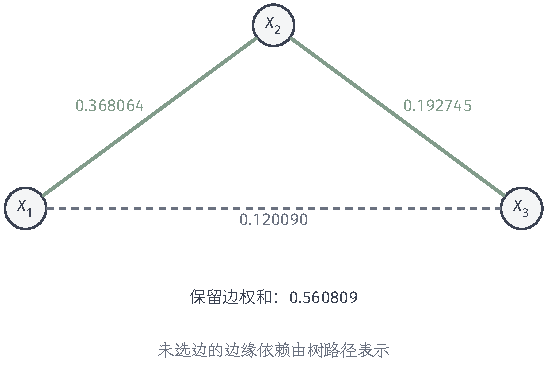
\includegraphics[width=92.650mm]{figures/06-probabilistic-graphical-models/03-learning/tikz/pgm-structure-learning-chow-liu/figure.pdf}
  \caption{计数表的互信息边权，单位为nat。最大权生成树保留实线两边，虚线是未选边。这个构造的经验分布恰好属于树族，因此可以精确复原；一般数据得到的是最佳树近似。}
  \label{fig:pgm-structure-learning-chow-liu}
\end{figure}

选$1$为根，根概率为$p(X_1=1)=0.5$，两条边的翻转概率为$0.1$、$0.2$。模型给出$\widehat p_{\mathcal{T}}(0,0,0)=0.5\times0.9\times0.8=0.36$；平均对数似然$-3\log2+0.368064+0.192745=-1.518633$，与前面评分计算相符。

证明中的正单点边缘用于保证条件概率分母有定义。零计数时可限制到经验支持，对从未出现的配置任选归一化条件表，并以$0\log0=0$延伸似然。若引入平滑伪计数，比较目标就随之改变。一般离散树的自由参数总数为
\[
  \sum_i(r_i-1)+
  \sum_{\{i,j\}\in E_{\mathcal{T}}}(r_i-1)(r_j-1).
\]
节点状态数相同等条件下，各树才有同一参数维数。状态数不同也不影响Chow--Liu对树族似然的精确优化，但BIC需扣除随边变化的参数惩罚，边权应作相应调整。

树约束同时简化学习与推断，也排除了环和不可约高阶作用。总体分布超出树族时，算法仍只能返回最佳树近似；互信息差异小时，抽样波动可能改变所选边。零权边也可能仅用于连接全节点，允许森林并惩罚边数则可保留断开的部分。

\subsection{高斯图结构学习}
\label{sec:pgm-structure-learning-gaussian}

对连续变量，高斯分布给无向结构学习带来一个极其优美的对应关系：联合高斯密度由协方差矩阵$\bm\Sigma$决定，但其逆矩阵$\bm K=\bm\Sigma^{-1}$（称为精度矩阵）的元素直接编码条件独立——精度矩阵里$K_{i,j}=0$，恰好等价于“给定其余所有变量后$X_i$与$X_j$独立”。直观上，$K_{i,j}$衡量的是把所有其他变量的影响都扣除后，$i,j$之间残留的直接关联；这一项为零，说明两者的相关完全可以由其余变量解释，它们之间不必有边。于是“学高斯无向图结构”被转化为“估计一个稀疏的精度矩阵”，这正是稀疏化方法可以大显身手的地方。要特别注意别和协方差混淆：$\Sigma_{i,j}=0$表示的是（不给定任何变量时的）边缘独立，而$K_{i,j}=0$才是条件独立，两者说的不是一回事。连续变量的条件依赖在高斯情形也有简洁表示。取$\bm{X}\sim\mathcal{N}(\bm{\mu},\bm{\Sigma})$、$\bm{\Sigma}\succ0$，\term{精度矩阵}（precision matrix）$\bm{K}=\bm{\Sigma}^{-1}$的零元素满足
\[
  X_i\perp X_j\mid\bm{X}_{V\setminus\{i,j\}}
  \quad\Longleftrightarrow\quad K_{i,j}=0.
\]
协方差零表示高斯边缘独立，精度零表示给定其余变量后的独立，二者约束不同。离开高斯分布后，逆协方差一般也失去这项条件独立解释。

由样本计算$\widehat{\bm{\Sigma}}=n^{-1}\sum_r(\bm{x}_r-\overline{\bm{x}})(\bm{x}_r-\overline{\bm{x}})^{\top}$，高斯负对数似然去常数并缩放后成为$-\log\det\bm{K}+\operatorname{tr}(\widehat{\bm{\Sigma}}\bm{K})$。直接把样本协方差求逆得到的精度矩阵通常是稠密的：由于抽样波动，几乎每个元素都只是很小、却不恰好为零，于是对应的图会变成全连接，没有揭示出真正的结构。要让无关的$K_{i,j}$被精确压成零，可以在高斯似然上加一个促使稀疏的$\ell_1$惩罚，这就是图Lasso；它同时完成“拟合高斯分布”和“筛出直接相连的边”两件事。小样本协方差可能奇异，直接求逆通常也不给稀疏零模式。对各变量样本方差严格为正的情形，\term{图Lasso}（graphical lasso）取$\lambda>0$，用非对角稀疏惩罚估计正定精度矩阵：
\begin{equation}
  \widehat{\bm{K}}
  =\argmin_{\bm{K}\succ0}
    \left\{-\log\det\bm{K}
      +\operatorname{tr}(\widehat{\bm{\Sigma}}\bm{K})
      +\lambda\sum_{i\ne j}|K_{i,j}|\right\}.
  \label{eq:pgm-structure-learning-glasso}
\end{equation}
上述样本方差与正惩罚条件保证唯一的有限正定最优解。若取$\lambda=0$，则需$\widehat{\bm{\Sigma}}\succ0$，最优解为其逆矩阵；零样本方差的变量应先移除或另行建模。

惩罚跳过对角，同时计算两个对称非对角元；只对$i<j$求和的实现需要换算$\lambda$。正定约束保持合法密度，$\ell_1$项允许估计出现精确零。目标是凸函数，可以用凸优化方法求解，抽样误差及选边正确性仍需统计条件\scite{pgm-structure-learning-friedman2008}

还可从每个节点的条件预测选择邻居。高斯条件均值为
\[
  \mathbb{E}[X_i\mid\bm{X}_{-i}]
  =\mu_i+\sum_{j\ne i}
    \left(-\frac{K_{i,j}}{K_{i,i}}\right)(X_j-\mu_j),
\]
$-i$表示其余全部节点，回归系数的非零模式因而对应邻居。分别作稀疏回归后，两端可能对同一边作不同选择；OR取并集，较多保留边，AND取交集，较少保留边。联合密度还需对称正定的精度矩阵，因此各节点独立回归后应继续检查或拟合相容参数。

例如取以下精度与协方差：
\[
  \bm{K}=
  \begin{pmatrix}
    2&-1&0\\
    -1&2&-1\\
    0&-1&2
  \end{pmatrix},
  \qquad
  \bm{\Sigma}=\frac14
  \begin{pmatrix}
    3&2&1\\
    2&4&2\\
    1&2&3
  \end{pmatrix}.
\]
两矩阵相乘为单位阵，精度矩阵顺序主子式为$2,3,4$，故正定。$\Sigma_{1,3}=1/4$显示边缘相关，$K_{1,3}=0$则说明给定$X_2$后独立。节点$1$仅回归到$X_2$，系数$1/2$；节点$2$对两端的系数也均为$1/2$，得到同一链。实际调参应按用途评价$\lambda$，预测误差最小与精确选边可能需要不同取值。

\subsection{离散与高阶Markov网络结构学习}
\label{sec:pgm-structure-learning-discrete}

树和高斯特例之所以好算，是因为只需要决定成对的边；但一般离散分布里，变量之间可能存在“三个变量才一起出现、任何两个单独看都独立”的高阶相互作用，这种结构无论怎么连成对边都表达不出来。因此一般离散无向模型的结构学习必须直接选择作用在任意变量子集上的特征（团），候选数量与归一化成本都随之上升。一般离散分布需要直接选择相互作用。先规定特征字典$\{f_a(\bm{x}_{C_a})\}$，$C_a\subseteq V$表示每个特征涉及的节点，再用有限状态的正指数模型表示概率：
\[
  p_{\bm{\theta}}(\bm{x})
  =\exp\!\left\{\sum_a\theta_a f_a(\bm{x}_{C_a})
                    -A(\bm{\theta})\right\}.
\]
参数的非零模式决定哪些相互作用参与模型。同一作用域有多项编码时，可用组稀疏惩罚共同选取；编码需可识别或有对比约束，使零系数具有确定含义。高阶因子的作用域在无向图中成为团，因此因子集合还能区分同一边图中的不同高阶关系。

用$\widehat{\mathbb{E}}[f_a]$表示经验特征均值，取$\lambda>0$并惩罚全部参数，完整似然的稀疏估计为
\[
  \min_{\bm{\theta}}\left\{
    A(\bm{\theta})-\sum_a\theta_a\widehat{\mathbb{E}}[f_a]
      +\lambda\lVert\bm{\theta}\rVert_1\right\}.
\]
正惩罚使参数趋于无穷时目标发散，从而存在有限最优参数。取$\lambda=0$时，需另查无罚最大似然估计是否存在；某些经验零频率会使目标仅在参数趋于无穷时逼近下确界。

梯度含模型期望，每轮都要进行推断；大团或大树宽会反复增加这项成本。\term{伪似然}（pseudolikelihood）改用各节点条件概率的乘积$\prod_{r,i}p_{\bm{\theta}}(x_{r,i}\mid\bm{x}_{r,-i})$。它只在单节点状态上归一化，可绕过全局配分函数；评价其统计效率与有限样本性质时，需要针对这个替代目标分析。

在成对Ising模型中，取$x_i\in\{-1,1\}$，局部场$u_i=b_i+\sum_{j\ne i}J_{i,j}x_j$汇总其他节点的作用。单点条件对数赔率为
\[
  \log\frac{p(X_i=1\mid\bm{x}_{-i})}
                {p(X_i=-1\mid\bm{x}_{-i})}=2u_i.
\]
该对数赔率使邻域估计化为稀疏逻辑回归。共同优化对称参数$J_{i,j}=J_{j,i}$时，条件概率来自同一联合模型；逐节点分别拟合时，还要协调两端选边与参数。直接搜索因子也可使用精确、近似或伪似然评分，应明确实际比较的目标。

成对边缘还可能隐藏高阶关系。以下正分布给出一个三变量反例：
\[
  p(x_1,x_2,x_3)
  =\frac{\exp(\theta x_1x_2x_3)}{8\cosh\theta},
  \qquad x_i\in\{-1,1\},\quad \theta\ne0.
\]
消去任一变量，分子变为$2\cosh\theta$，每对边缘都是$1/4$，故成对互信息为零。三阶矩却满足$\mathbb{E}[X_1X_2X_3]=\tanh\theta\ne0$，给定$X_3$后两端仍有相互作用。这个处处正的分布需要三阶特征，说明成对独立不足以推出联合独立。若允许大小至多$m$的作用域，候选子集数为$\sum_{\ell=1}^{m}\binom d\ell$，每个离散作用域还可能有多个参数，搜索及样本成本随之增长。

\subsection{潜变量结构的学习}
\label{sec:pgm-structure-learning-latent}

到此为止都假设数据里的变量就是全部相关变量。但现实中观测到的一大堆变量可能只是少数几个\emph{未观测共同原因}的结果——例如若干传感器读数相关，仅仅因为它们都受同一个隐藏的环境温度驱动。若不知道这个隐变量、直接在观测变量间学图，就会在本无直接关系的变量之间连出稠密的一团边。结构学习因此还要区分：哪些依赖在把隐变量考虑进来后仍真实存在，哪些依赖只是共同隐变量投下的“影子”。稠密观测关系还可能由共同隐变量产生。此时直接恢复观测边缘图，会把共同隐变量造成的关系与观测变量之间的条件关系混在一起。结构学习需要进一步判断：哪些依赖在给定潜变量后仍然保留，哪些依赖可以由少量共同潜在方向解释。将联合高斯节点分为观测集合$O$和潜变量集合$H$，按两组分块精度矩阵。积分潜变量或对二次型配方后，观测边缘的精度为
\begin{equation}
  \begin{aligned}
    \bm{K}_{\mathrm{marg}}
      &=(\bm{\Sigma}_{O,O})^{-1}\\
      &=\bm{K}_{O,O}
        -\bm{K}_{O,H}\bm{K}_{H,H}^{-1}\bm{K}_{H,O}\\
      &=\bm{S}-\bm{L}.
  \end{aligned}
  \label{eq:pgm-structure-learning-schur}
\end{equation}
$\bm{S}=\bm{K}_{O,O}$表示给定潜变量后的条件精度；$\bm{L}\succeq0$且秩至多$|H|$表示边缘化带来的修正。条件图稀疏、有效潜变量少时，这构成常称的\term{稀疏加低秩分解}（sparse plus low-rank decomposition）。名称强调两种结构，按此处半正定约定实际以减法组合。

取$X_i=Z+\varepsilon_i$，$i=1,2,3$，并令$Z,\varepsilon_1,\varepsilon_2,\varepsilon_3$相互独立且均为标准高斯。给定$Z$后三个观测独立；积分$Z$后协方差为$\bm{I}+\bm{1}\bm{1}^{\top}$，其逆可直接验证为
\[
  \bm{K}_{\mathrm{marg}}
  =\bm{I}-\frac14\bm{1}\bm{1}^{\top}.
\]
所有非对角元为$-1/4$，所以观测条件图完整，而$\bm{S}=\bm{I}$、$\bm{L}=\bm{1}\bm{1}^{\top}/4$只有一个潜在修正方向。边缘依赖与给定共同潜变量后的独立，描述的是不同条件分布。

根据观测样本协方差$\widehat{\bm{\Sigma}}_{O,O}$，取$\lambda>0$，可以同时拟合这两种结构：
\begin{equation}
  \begin{aligned}
    \min_{\bm{S},\bm{L}}\quad&
      -\log\det(\bm{S}-\bm{L})
      +\operatorname{tr}\!\left(
           \widehat{\bm{\Sigma}}_{O,O}(\bm{S}-\bm{L})\right)\\
      &+\lambda\bigl(\gamma\lVert\bm{S}\rVert_1
                      +\operatorname{tr}(\bm{L})\bigr),\\
    \text{满足}\quad&\bm{S}-\bm{L}\succ0,\qquad \bm{L}\succeq0.
  \end{aligned}
  \label{eq:pgm-structure-learning-sparse-low-rank}
\end{equation}
$\lVert\bm{S}\rVert_1$逐元素求绝对值，包含对角；$\gamma>0$调节稀疏与低秩惩罚的相对强度。正惩罚控制精度矩阵及潜变量修正的增长，使有限正定最优解存在。取$\lambda=0$时，仍需观测样本协方差正定，边缘精度的最优解才是其逆矩阵，$\bm S$与$\bm L$的分解则可能不唯一。

半正定矩阵的核范数等于迹，所以第二项鼓励低秩。该凸程序的恢复保证还需两类结构足够可区分，例如潜变量作用分散于较多观测节点，避免低秩项本身也高度稀疏\scite{pgm-structure-learning-chandrasekaran2012}

若某分量同时稀疏、低秩，它可以在两项间移动而不改变差，精确边缘精度也可能无法确定唯一分解。满足识别条件时，$\bm{L}$的秩表示有效潜在维数，潜变量的物理个数、旋转与含义仍需额外信息。完整潜变量图、条件图$\bm{S}$和边缘观测图$\bm{K}_{\mathrm{marg}}$因此应分别解释；低秩分解回答统计结构问题，尚未识别潜在因果机制。

\section{因果发现}
\label{sec:pgm-structure-learning-causal}

本章前几节学到的图，严格说只表示变量在\emph{被动观测}下的联合分布；而等价类的存在意味着，光凭这种分布往往无法确定箭头方向。但在很多决策问题里我们真正想问的是“如果人为去改变某个变量会怎样”——降低温度会不会真的减少故障？这是一个\emph{干预}问题，需要把箭头读作因果机制。本节就讨论：在观测数据基础上，需要补上哪些假设或哪类实验数据，才能把结构（哪怕部分地）解释为因果结构。到这里，图用于表示联合分布。若要预测外部改变某变量的后果，还需给局部关系赋予干预含义。接下来比较不同信息与假设能识别到什么结构，让输出对应可以成立的因果结论。

\subsection{因果假设与识别目标}
\label{sec:pgm-structure-learning-causal-assumptions}

要把观测到的图当因果图用，必须先明确几条无法仅靠数据证明、需要由问题背景背书的假设。最核心的是因果Markov性与忠实性这一对：前者保证“因果结构会产生我们能观测到的独立约束”，后者保证“观测到的独立都能归因于结构”，两者合起来才允许从独立性反推因果方向。因果Markov性要求每个变量在给定其直接原因后，与非后代独立；忠实性则要求分布中的条件独立都由图上的d-分离解释。前者从机制导出独立约束，后者支持从独立关系反推图，但观测等价仍会限制方向识别（参见\BookSectionRef{sec:causal-structure-discovery}{卷2《数学准备：概率、因果与决策》第3章“因果响应”第3.6节“因果生成结构的推断”}）。本节在这些条件下考察可识别输出，再说明潜在混杂、函数形式及干预如何提供不同信息。

当前变量是否覆盖共同原因，也影响图的解释。\term{因果充分性}（causal sufficiency）要求它们的共同原因都已观测，即当前模型没有遗漏潜在混杂。它只针对所选节点集合，通常还需无环过程、已声明的数据环境及适当处理选择偏差。以函数形式识别更多方向时，还要加入相应线性、噪声独立或非高斯条件；搜索方法使用这些假设，却不能自行验证它们成立。

因果充分、无环且忠实时，观测独立信息一般确定CPDAG。一旦允许存在未观测的共同原因，CPDAG就不够用了：它无法表达“两个观测变量的相关其实来自一个潜混杂”这种关系，而把隐变量显式画出来又会让图无限膨胀、且我们根本不知道有几个隐变量。需要一种只画观测变量、却能用不同端点记号同时表达“祖先方向”和“由潜变量造成的混杂”的图。允许潜变量后，需表示边缘化留下的关系。\term{最大祖先图}（maximal ancestral graph, MAG）用有向、双向及处理选择偏差时的无向边表达观测独立性，省去潜变量的显式细节。合法图无有向环；箭头端不能是另一端的祖先，无向边的端点不能再接指入箭头。“最大”表示每对不相邻节点都能由某组观测量分离。对应的\term{m-分离}（m-separation）按两侧箭头辨认路径碰撞点：活跃路径要求非碰撞点不在条件集中，每个碰撞点自身或某个后代在条件集中；两端没有活跃路径时才被分离。

多张MAG也可能具有相同独立关系，\term{部分祖先图}（partial ancestral graph, PAG）保留这类图共同的端点信息。尾端和箭头端为类内不变标记，圆圈表示端点尚未确定，边本身仍存在。无选择偏差时，$i\to j$表示祖先关系，$i\leftrightarrow j$排除互为祖先且与潜在混杂相容，$i\mathbin{\circ\!\!\to}j$只确定$j$端箭头。这些标记表达祖先与独立性的不确定性，未给出直接因果机制、双向反馈或潜变量的具体个数和连接\scite{pgm-structure-learning-zhang2008}

\subsection{基于观测数据的因果发现}
\label{sec:pgm-structure-learning-observational}

先看在不做实验、只有观测数据时，靠不同强度的假设最多能把方向确定到什么程度：最基本的PC/GES只能给CPDAG；允许潜在混杂的FCI给更保守的PAG；而借助“线性+非高斯噪声”等函数形状假设，LiNGAM、ANM等方法有时能打破观测等价、唯一确定方向——代价是假设强得多。PC与GES得到的统计等价类，要在因果假设下才能解释为因果等价类（参见第~\ref{sec:pgm-structure-learning-directed}节）。PC在因果Markov性、忠实性、充分性、无环性及准确独立判定下返回CPDAG，有限样本返回其估计。GES则需要评分等价、可分解且局部一致，真实分布忠实于候选有向图，并满足固定维大样本条件。这里局部一致性具体指：样本足够多时，评分奖励补上遗漏依赖，惩罚多余依赖；在这些条件下等价类搜索可恢复CPDAG。

潜在混杂会改变需要检查的分离集合。\term{快速因果推断算法}（fast causal inference, FCI）扩展PC的搜索范围并采用祖先图定向规则，在相应Markov性、忠实性和准确独立信息下输出PAG。标准框架还可处理声明的选择机制。无限观测数据也可能只确定这个部分对象，圆圈应继续保留；完整规则及识别范围见Zhang的研究\scite{pgm-structure-learning-zhang2008-completeness}

分布形状可以提供独立关系之外的方向信息。\term{线性非高斯无环模型}（linear non-Gaussian acyclic model, LiNGAM）以独立扰动驱动各节点：
\[
  X_j=\sum_{i\in\operatorname{pa}(j)}b_{j,i}X_i+\varepsilon_j,
\]
图取无环，扰动相互独立、非高斯且方差有限非零，并排除未观测混杂。令$B_{j,i}=b_{j,i}$，递归方程给出$\bm{X}=(\bm{I}-\bm{B})^{-1}\bm{\varepsilon}$。这里用到的\term{独立成分分析}（independent component analysis, ICA）本是一种信号分离技术（经典例子是把多个麦克风录到的混合人声按“各声源相互独立”还原出来）；在LiNGAM中它被借来从观测变量的混合中分离出相互独立的非高斯扰动；非高斯性用来区分各个扰动来源，无环约束再用来解决“分离出的分量该对应到哪个变量”的排列歧义，于是可在模型条件下识别超出MEC的方向。线性高斯分布缺少这种方向信息，识别结论依赖所保留的非高斯条件\scite{pgm-structure-learning-shimizu2006}

非线性函数也可能使方向不对称。\term{加性噪声模型}（additive noise model, ANM）取$Y=f(X)+\varepsilon$、$\varepsilon\perp X$；在满足相应光滑性、非退化和可识别性条件的模型中，反向无法同时写成$X=g(Y)+\eta$、$\eta\perp Y$。因此可比较输入与拟合残差的独立性，而不只比较回归误差。多变量形式还需递归机制及独立扰动；线性高斯等双向可表示情形属于识别例外\scite{pgm-structure-learning-peters2014}

\subsection{基于干预数据的因果发现}
\label{sec:pgm-structure-learning-interventional}

既然纯观测数据困在等价类里，打破僵局最直接的办法就是做实验：主动去\emph{设置}（干预）某个变量的值，而不只是观察它。干预会切断该变量与其自然原因之间的联系，从而制造出观测数据中不存在的不对称——三张观测等价的图，在同一个干预下往往给出明显不同的预测。观测和干预的差别可以继续用计数表说明。观测$X_2=1$时，$X_1=1$的频率为$0.9$；外部设置$X_2$却改变了数据产生方式。正向链$X_1\to X_2\to X_3$中，改变中间变量不影响其上游$X_1$；分叉$X_1\leftarrow X_2\to X_3$中，$X_1$随之改变。这类实验能区分相同被动观测支持的机制。

为计算这种改变，\term{完美干预}（perfect intervention）替换目标节点的机制、切断它对原父节点的依赖，同时保持其他机制。取已知目标集合$I\subseteq V$，各目标独立随机化并使用外部规定的$q_i^I$，干预分布为
\begin{equation}
  p^I(\bm{x})
  =\prod_{i\in I}q_i^I(x_i)
   \prod_{j\notin I}
      p(x_j\mid\bm{x}_{\operatorname{pa}_{\mathcal{G}}(j)}).
  \label{eq:pgm-structure-learning-intervention}
\end{equation}
图上删去进入$I$的全部箭头，得到$\mathcal{G}^{[I]}$；$I=\varnothing$给回观测环境。固定目标值可作为退化干预。以独立信息刻画等价类时，需要足够支持的随机化或覆盖相关取值的实验，以免变量固定造成额外退化。

记目标集合族为$\mathcal{I}$。若每个节点至少在一个环境未受干预，该族称为\term{保守的}（conservative），包含观测环境即满足。给定目标及完美干预规则后，允许相同多环境分布族的有向无环图构成\term{干预Markov等价类}（interventional Markov equivalence class, I-MEC）。各环境共享非目标机制，因而这里比较的是协调的多环境模型。

在保守目标族及相应正性条件下，两图干预等价恰好要求观测Markov等价，并且每个$I\in\mathcal{I}$下的删入边图具有相同骨架。也可用观测骨架与v-结构相同，再比较各干预图的Markov等价关系来刻画。\term{干预本质图}（interventional essential graph）把I-MEC共同方向画成箭头，其余边保持无向。干预细分了观测MEC，但目标不足时仍可能保留多张候选图\scite{pgm-structure-learning-hauser2012}

将三种观测等价图都拟合到同一二值表，再作$\operatorname{do}(X_2=1)$。正向链预测$(p(X_1=1),p(X_3=1))=(0.5,0.8)$，分叉为$(0.9,0.8)$，反向链为$(0.9,0.5)$；仅观测$X_2=1$时，三者却都给$(0.9,0.8)$。图~\ref{fig:pgm-structure-learning-intervention}展示这组差异：在给定总体假设下，覆盖$X_2$两种取值的完美干预足以区分它们。有限实验还需评价频率估计误差。

\begin{figure}[!t]
  \centering
  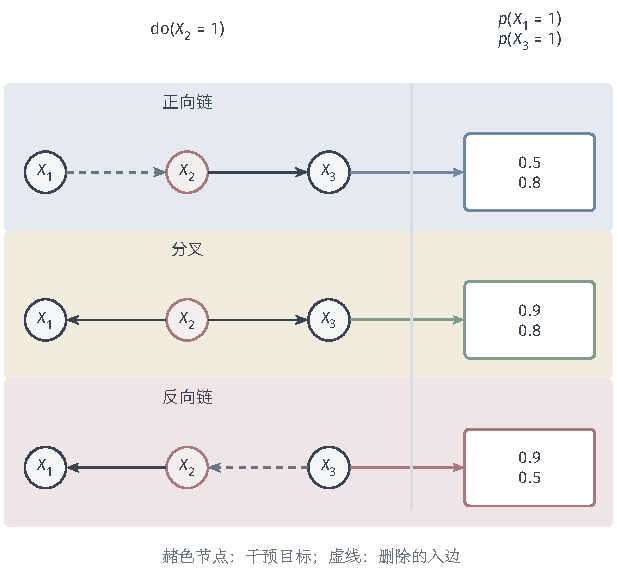
\includegraphics[width=104.405mm]{figures/06-probabilistic-graphical-models/03-learning/tikz/pgm-structure-learning-intervention/figure.pdf}
  \caption{干预$X_2$对同一观测MEC的三种预测。蓝、黄、红横带依次为正向链、分叉、反向链，右侧概率框及连接箭头对应各结构的预测。实线保留非目标机制，虚线表示切断的入边；在给定三节点设定下，预测差异提供方向信息。}
  \label{fig:pgm-structure-learning-intervention}
\end{figure}

\term{贪心干预等价搜索}（greedy interventional equivalence search, GIES）直接在干预本质图空间比较I-MEC，采用前向、后向及转向操作。每条记录需带目标标签$I_r$；目标随机化分布已知或独立于候选图时，去掉共同常数后的机制对数似然为
\[
  \ell(\mathcal{G},\bm{\theta})
  =\sum_{r=1}^{n}\sum_{j\notin I_r}
       \log p_{\bm{\theta}_j}
          (x_{r,j}\mid\bm{x}_{r,\operatorname{pa}(j)}).
\]
目标节点的观测不用于拟合它的原机制，仍可进入子节点的机制拟合。各机制可用样本数不同，惩罚评分需要体现这种多环境设定。GIES据此汇合观测与干预证据；具体搜索最优性及因果恢复仍须结合评分、样本和模型条件分析。

未知目标时，环境标签只说明有机制变化，还需限定哪些机制可变、变化是否可检测及其余机制如何保持，再联合推断目标。软干预只改机制的一部分而保留父依赖，也需要修改删边表示和I-MEC定义。执行不依从、目标不完全、非目标机制漂移或潜在混杂都会改变识别范围，应使用与这些条件相容的模型。

已有候选还可用于决定下一次实验。\term{主动实验设计}（active experimental design）在可执行且满足预算的目标中，选择预计最能区分候选的干预；三节点例子的中间节点就是一项选择。预期后验熵下降、待定端点减少或科学查询的区分度都可作为准则，并需计入成本。这些预期仍依赖当前模型和机制不变假设，实验实施后的证据要另外评价。

表~\ref{tab:pgm-structure-learning-causal-routes}把信息、假设和输出放在同一口径下比较。路线可以交叉：ANM可使用回归及独立检验，连续优化也可处理特定函数模型。识别能力由数据和模型条件决定，求解工具规定如何利用这些信息。

\begin{table*}[htbp]
  \centering
  \small
  \begin{tabularx}{\linewidth}{@{}lXX@{}}
    \toprule
    路线 & 关键条件与信息 & 理想识别对象及限制 \\
    \midrule
    PC & 无环、因果充分、Markov且忠实；准确独立性信息 & CPDAG；不决定类内可逆方向 \\
    GES & 相应充分有向图模型；评分等价、可分解、局部一致 & 大样本下CPDAG；不是一般贪心搜索的保证 \\
    FCI & 允许潜在混杂；相应Markov性、忠实性及选择机制假设 & PAG；不是潜变量完整图 \\
    LiNGAM & 线性无环、独立非高斯扰动、无潜在混杂 & 模型条件下单个有向图；依赖分布形状 \\
    ANM & 独立加性噪声、无混杂及特定可识别性条件 & 满足条件时单个有向图；存在双向可表示例外 \\
    GIES & 已知目标的完美干预、无混杂、机制不变、相应评分 & 搜索I-MEC；并非一般全局最优保证 \\
    \bottomrule
  \end{tabularx}
  \caption{不同假设下的识别目标。表列理想输出以总体条件成立为前提；实际估计还包含抽样、拟合与搜索误差，因此需同时说明假设和计算过程。}
  \label{tab:pgm-structure-learning-causal-routes}
\end{table*}

\subsection{因果发现的边界}
\label{sec:pgm-structure-learning-causal-limits}

因果发现的结论有多可信，必须把“不确定”按来源分清楚，因为三种不确定性的补救办法完全不同：样本太少带来的统计误差靠补数据解决；假设错了会让更多数据反而更坚定地指向错误的图；而总体层面的不可识别则再多数据也无用、只能靠新假设或新实验。不确定性需要按来源判断。样本误差使检验和评分偏离总体结果，增加同类记录有机会降低它。假设错误可能让更多数据稳定地支持错误图，例如有混杂却使用充分性模型。总体不可识别则意味着多个候选在所有允许资料下都产生同一分布，需要增加信息才能区分。这三种情况分别指向补样本、改模型及设计实验。

等价类中的未定向边和PAG圆圈保留的是资料尚未确定的信息。领域知识可以排除候选，应标明它贡献的方向；函数形式可以缩小等价范围，也需核验对应假设。稀疏、有向且重复得到的图仍只说明特定流程的结果，因果解释需要这些额外依据。

结构发现之后，干预效应是否可计算仍是另一项识别问题，do演算和反事实查询有各自定义及条件。本节得到的部分结构为这些查询提供约束，具体效应和个体反事实还需按对应问题分析。

\section{算法分析}
\label{sec:pgm-structure-learning-analysis}

参数学习的评价相对直接（估计值离真值多近、预测准不准），结构学习的评价却更微妙：算法可能恢复错了方向却恰好预测得不错，也可能在有限样本上不稳定，还可能因为算不动而只找到局部最优。系统地评价一种结构学习方法，要分别回答三个不同层面的问题。评价结构学习可以沿三个问题展开：候选图及局部函数能表示哪些分布；搜索能否找到目标候选、以多少计算完成；有限样本下选出的结构与预测能否接近总体目标。下面分别检查统计一致性、计算成本和评价协议，使“最优”“一致”与“稳定”各有明确对象。

\subsection{统计一致性与有限样本误差}
\label{sec:pgm-structure-learning-consistency}

首先要区分“估计得准不准”和“问题本身能不能确定”。结构学习的一致性必须针对一个\emph{可识别的目标}来谈——当观测数据只能确定CPDAG时，要求算法稳定地恢复出某一张特定方向的有向图本身就不合理，正确目标应是那个等价类。先把可识别目标记为$\mathcal{C}^{*}$，例如CPDAG；\term{结构一致性}（structural consistency）要求$\mathbb{P}(\widehat{\mathcal{C}}_n=\mathcal{C}^{*})\to1$。目标必须与可用信息匹配。真实分布超出树族时，Chow--Liu可以趋向最佳树近似；图Lasso参数误差趋零时，精确零模式还需非零信号与零之间有足够间隔。

PC需要全部相关独立判定同时正确。若检验集合大小为$M$、每项错误概率至多$\delta$，联合界给出至少一项检验出错的概率至多$M\delta$，无需检验独立。自适应选择时应覆盖全部可能用到的检验，而非事后只数执行次数。若要整体错误随$n$消失，固定显著性水平通常不足，还需合适阈值序列及功效条件。

最弱依赖往往决定可恢复程度。高斯偏相关小于估计波动时难以检出；离散条件集扩大后，每个配置的记录更少。稀疏图有助于限制条件集，同时仍需控制最大度、状态数、协方差条件数或最小信号，才能给出具体一致性结论。

BIC比较也依赖固定维、正确模型和正则条件。遗漏依赖通常带来随$n$线性增长的似然损失，多余参数的随机拟合收益通常仅为有界概率量级，$\log n$惩罚据此区分两者。这个理由说明评分的候选比较；搜索若未到达相关模型，还需另外控制搜索误差。潜变量奇异或维数增长时，应重查渐近尺度。

树的稳定性可以由边权间隔直接说明。取$d\geq3$且总体最大权生成树唯一，对非树边$e$与其连接路径上的树边$f$，定义
\[
  \Delta=\min_{e\notin E_{\mathcal{T}^{*}}}
             \min_{f\in\operatorname{path}_{\mathcal{T}^{*}}(e)}
             \{I_f-I_e\}.
\]
若$\Delta>0$且所有互信息估计误差小于$\Delta/2$，非树边与路径边的次序保持，最大权树也保持。教学例子中间隔约为$0.072654$，等于较小两条互信息的差。零间隔可能容许多棵最优树，分布预测相近时具体选边仍可能变化。

\subsection{计算复杂度与可扩展性}
\label{sec:pgm-structure-learning-complexity}

一致性回答“样本足够多时能否恢复对的结构”，但实践中还要问“要花多少计算、规模一大还算不算得动”。结构学习的开销主要来自在巨大图空间里反复做检验或评分，下面按主要算法分别给出规模量级。计算成本要按实际搜索规模估计。PC枚举条件集并逐项检验；整个过程中候选邻域至多$q$时，粗略检验数为$O(d^2 2^q)$，总时间还乘单次检验成本。误保留边会增大候选邻域，故$q$未必等于真实最大度。FCI扩大了分离集搜索范围，也增加相应运算。

离散有向图可缓存局部评分，候选父集数量仍可能指数增长。预计算最佳父集表后，常见动态规划递推约需$O(d2^d)$时间，表的准备及内存另计；整数规划的分支搜索同样可能指数增长。局部搜索每轮约检查$O(d^2)$个移动，总成本还取决于轮数、无环检查及拟合，需与单轮操作数分开。

状态数有界时，Chow--Liu以$O(nd^2)$时间汇总成对计数，再以稠密Prim的$O(d^2)$或排序Kruskal的$O(d^2\log d)$求树。固定树上的有限状态边缘推断随节点数线性增长。这两项计算收益来自树约束，也伴随其表示能力限制。

稠密NOTEARS每次残差乘法约需$O(nd^2)$，矩阵指数通常需$O(d^3)$规模的线性代数，总时间还乘内部优化及惩罚更新轮数。图Lasso有矩阵更新成本，凸性则方便检查求解误差；逐节点回归易并行，联合参数相容性需继续处理。高阶离散评分还可能反复计算配分函数。限制父集或作用域时，应说明节省的计算和排除的候选。

\subsection{结构评价与稳定性}
\label{sec:pgm-structure-learning-evaluation}

有了已知真值的仿真数据，就能直接量化“学出的图和真图差多远”，但要注意骨架对错与方向对错应分开计分，并且当目标本就是等价类时，不应因为可逆方向没猜中而扣分。仿真有已知生成结构时，可分别测量骨架与方向。骨架精确率为正确边数除以预测边数，召回率为正确边数除以真实边数，零分母规则需预设。方向评价需说明是否计入漏边。若资料只能识别CPDAG，应以该类为目标，既不因未选中某代表的可逆方向罚分，也不把偶然猜中当作识别收益。

最常用的单一指标是直接数“要把学出的图改成真图，至少做多少次边的增删改”。\term{结构Hamming距离}（structural Hamming distance, SHD）就计量估计图变到目标图所需的边编辑数，数值为零表示两图完全一致；常见约定将加边、删边、反向各计1，也有把反向计为删加两步的实现，比较时需固定口径。CPDAG评价先将生成有向图转为等价类，再比较邻接、被迫方向和未定向状态；PAG还需比较圆圈、尾端及箭头端。

真实数据通常没有一张“真图”可供对照打分。退而求其次的办法是考察结果的\emph{稳定性}：若换一批略有不同的样本，学出的图就面目全非，说明这些边并不可靠；若某些边在各种扰动下都反复出现，则更可信。实现这种扰动的标准手段是对原数据有放回地重复抽样。真实记录缺少标准答案时，可测量结果对重采样的敏感性。\term{自助重采样}（bootstrap）从$n$条独立记录有放回抽$n$条，重复拟合$B$次，将边出现频率写为
\[
  \widehat\pi_{i,j}
  =\frac1B\sum_{b=1}^{B}
       \mathbf{1}\{\{i,j\}\text{在第}b\text{次结果中相邻}\}.
\]
方向需另计频率，并声明分母取全部重复还是该边出现的重复。CPDAG未定向边应保留该状态；各轮是否重做筛选与调参，也影响所测流程。多环境资料在环境内重采样，相关序列则按适当块抽样，使评价单位符合数据依赖。

重采样频率表示流程对数据扰动的敏感性；错误先验或模型假设也可能产生稳定结果，因此它不同于结构后验及因果真实性概率。还可比较合理正则、检验和模型设置，并在未参与选图与调参的记录上报告平均预测对数概率或对数密度，值越大表示给真实观测的预测支持越高。这项预测评价仍未验证因果方向。

领域知识也可明确限制候选。禁止$i\to j$就排除$X_j$父集中含$X_i$的选项，必选$i\to j$则保留包含$X_i$的父集；时间顺序排除逆时间箭头。搜索前需检查约束相容且无环；等价类结果还应区分数据确定与知识补充的方向，并相对于加入同一知识后的识别目标评价。

\section{本章小结}
\label{sec:pgm-structure-learning-summary}

从记录到图，需要分别判断局部独立证据、整体模型得分和合法空间搜索。检验说明哪些联系可由给定变量隔断，评分权衡拟合与复杂度，搜索组织候选比较。树之所以可精确求解，是因为最优似然化为互信息边权和；一般有向图和高阶无向模型还要承担更大的搜索或归一化成本。

同一张计数表可支持无向链、观测等价类及结构后验，却不能仅由频率选定因果方向。缺失观测引入后验统计量，潜变量边缘化可能使稀疏条件图变稠密；改变的不只是运算，也包括可识别对象。赋予结构因果解释时，需明确机制、混杂、忠实性和函数形式假设，才能判断结果是CPDAG、PAG还是干预等价类中的信息。

回到设备记录，数据能够帮助选择依赖表示，故障传播方向还需相应识别条件和干预依据。增加同类样本可以在相应统计条件下降低估计误差；改善搜索用于控制优化误差，修改假设用于处理模型偏差，总体观测等价则可能仍需新实验。因此报告结构时，应同时给候选范围、数据与干预条件、检验或评分、搜索限制及保留的不确定性。

接下来的模型以具体任务选择这些结构：分类、潜在分组和状态估计各有其表达与计算要求。静态有向模型把局部分解、推断和学习用于此类任务（参见第~\ref{chap:pgm-static-directed}章）。结构适合计算和预测时，潜变量的物理含义仍可能需要其他证据。

\paragraph{扩展阅读}
Koller与Friedman的教材进一步展开条件独立检验与评分搜索，可按本章的计数、等价类和搜索目标继续阅读。理解统计分解之后，再核对因果解释增加了哪些机制与识别条件\scite{pgm-koller2009}

\chapter{静态有向模型}
\label{chap:pgm-static-directed}

前三部分分别讲清了概率图模型的三件事：怎样用图\emph{表示}联合分布、给定图后怎样做\emph{推断}、以及怎样从数据\emph{学习}参数和结构。从本章开始的第四部分“模型”，要把这些工具组装到一个个具体的、有名有姓的模型上：每一种模型选定一种图结构和一族局部条件分布，前面学到的推断与学习算法就落到这张具体的图上。本章先从最基础也最常用的一类——\emph{静态有向模型}入手。“静态”指记录之间没有真实的时间先后假设，每条记录是某个时刻拍下的一张“快照”；“有向”指联合分布被写成一串局部条件概率的乘积。

同一个“多个传感器读数常常一起变化”的现象，其实可以在三个层次上追问，而这三个层次恰好对应本章的三条主线。最直接的一层是\emph{观测之间的依赖}：给定第一个读数，第二个读数如何分布（朴素贝叶斯、自回归模型）。更深一层是\emph{记录内部的潜在解释}：两个读数一起升高，会不会是因为背后有一个我们没直接测到的“工作状态”在共同驱动它们（混合模型、因子模型）。再往上，当记录来自不同工厂、不同文档时，还要问\emph{跨记录的共享}：哪些规律是各组通用的、哪些允许各组各自不同（层次模型、主题模型）。

两个传感器的读数经常一起升高。可以直接建模第二个读数在第一个读数给定时的分布，也可以引入未观测的工作状态，让它共同影响两个读数。前一种方法拟合观测间的条件关系，后一种方法还要推断工作状态，并将它从联合分布中汇总掉。若记录又来自不同工厂，还要说明哪些规律跨厂共享、哪些参数允许各厂不同。本章围绕观测间的直接依赖、记录内部的潜在解释和跨记录的共享，分析它们怎样决定学习目标、缺失值查询及相关性的解释。

有向模型将联合分布写成局部条件概率的乘积，概率语义见第~\ref{chap:pgm-directed}章。本章选取静态模型，展开这些局部函数以及相应的推断和学习计算。这里的依赖没有沿真实时间演化的假设。一条记录记为$\bm x\in\mathbb R^d$或离散取值向量，训练数据为$\bm x_1,\ldots,\bm x_n$，待估参数统一记为$\bm\theta$；有类别标签时，用$Y$表示图中的类别节点。

先从全部建模变量都可观测的直接分解开始，再加入离散或连续的潜变量，分析求和与积分怎样形成观测分布。随后将多个记录按组组织，说明共享上层变量与每项选择成分的不同结构。潜变量的取值类型和记录间的共享方式可以同时变化，因此模型比较分别考察这两类选择，以及它们带来的计算和解释代价。

\section{静态观测的有向建模问题}
\label{sec:pgm-static-directed-common}

本节固定全章反复使用的记号和两条共同计算：有向图怎样给出联合分布，以及引入潜变量后似然和后验为何都变成对潜变量的求和或积分。后续具体模型都是在这两条公式上选定不同的图结构和局部函数。记全部节点变量为$\bm V=(V_1,\ldots,V_m)$，图为$\mathcal G$，$\operatorname{pa}_{\mathcal G}(i)$表示节点$i$的父集，$\bm\theta$汇集局部参数。每个节点的条件分布在父变量固定时归一化，联合分布便按图写成
\begin{equation}
  p_{\bm\theta}(\bm v)
    =\prod_{i=1}^m
       p_{\bm\theta_i}(v_i\mid
          \bm v_{\operatorname{pa}_{\mathcal G}(i)}).
  \label{eq:pgm-static-directed-common-joint}
\end{equation}
离散节点使用条件概率，连续节点使用相应基准测度下的条件密度。无环性让各局部条件分布可以按拓扑序组合；其归一化依据见第~\ref{chap:pgm-directed}章。图规定允许使用哪些父变量，函数形式及参数则决定具体的候选分布，二者共同影响能够表达的观测关系。

如果整条记录中的建模变量都已观测，评价似然只需将记录代入这些局部条件分布。若将变量分成观测量$\bm X$和潜变量$\bm Z$，记录只提供$\bm x$，就要汇总所有可能的潜在解释：
\begin{equation}
  \begin{aligned}
    p_{\bm\theta}(\bm x)
      &=\int p_{\bm\theta}(\bm x,\bm z)
                    \,\mathrm d\mu_Z(\bm z),\\
    p_{\bm\theta}(\bm z\mid\bm x)
      &=\frac{p_{\bm\theta}(\bm x,\bm z)}
                    {p_{\bm\theta}(\bm x)}.
  \end{aligned}
  \label{eq:pgm-static-directed-common-marginal}
\end{equation}
$\mu_Z$在离散状态上取计数测度，因此积分表示求和；混合状态则采用对应的乘积测度。后验式要求观测边缘概率或密度为正。第一个式子用于评价观测似然，第二个式子用于判断一条记录的潜在状态；有向分解容易求值，并不意味着这两个汇总都容易计算。

设$n$条记录相互独立并使用同一组固定参数，观测对数似然是各记录对数概率或密度的和：
\[
  \ell(\bm\theta)=\sum_{j=1}^n\log p_{\bm\theta}(\bm x_j).
\]
参数学习需要提高这些记录的概率或密度；含潜变量时，后验期望可能参与EM或梯度计算，通用方法见第~\ref{chap:pgm-parameter-learning}章。一个共享随机上层变量还会在被积分掉后诱导记录间依赖，此时应评价整组记录的联合似然，不能继续套用独立记录的对数似然和。

下面的直接模型限制观测之间的父集或局部函数；有限混合与连续因子模型加入记录内部的潜在解释；层次与混合成员模型进一步规定组间共享和组内分配。它们改变的是不同层次的关系，可以组合使用。这里的箭头表达概率分解，不自动赋予因果含义；变量顺序也不等同于真实时间的演化。

\section{观测之间的直接依赖建模}
\label{sec:pgm-static-directed-direct}

给定一条完整记录，就能在各节点读取父变量的取值，并计算局部条件概率的乘积。局部分布各自归一化后，这个乘积已经是合法的联合分布。缺失某些取值时，还需对它们求和或积分，计算规模随缺失模式改变。这里不为解释记录额外加入随机状态，而是直接规定训练中可见节点的条件分布。类别已记录时，重点是类别内部的属性关系；没有指定类别时，重点是沿所选字段顺序描述完整记录密度。预测时类别未知，只改变查询，不会把训练中已观测的类别改称模型主动引入的潜变量。

\subsection{基于类别条件的属性建模}
\label{sec:pgm-static-directed-naive-tan}

类别条件建模需要在每个类别内估计读数规律。若直接存储全部属性组合，每类的条件表随属性数量迅速增长；先限制类内依赖，再在必要时保留一部分依赖，可以明确控制需要从数据估计的内容。

\subsubsection{朴素贝叶斯：用类内独立减少待估参数}
\label{sec:pgm-static-directed-naive}

给定设备类别和一批传感器读数，最自然的分类问题是：看到读数后，它属于哪一类的可能性最大？要直接估计“读数组合$\to$类别”的完整分布，需要列出所有属性组合的概率，属性一多，组合数指数爆炸、数据根本不够分。一个大胆而朴素的简化是：一旦把类别固定下来，就假设各个读数之间\emph{条件独立}——也就是认为同一类设备的各传感器读数是在类别已知后彼此独立地产生的。这个假设在现实中很少严格成立，却能把一个高维联合分布拆成若干一维分布的乘积，参数量和数据需求骤降，而且实践中分类效果常常出奇地好，这就是朴素贝叶斯。训练数据同时记录设备类别与传感器读数时，可以先估计各类的读数分布，再据新读数计算类别后验。\term{朴素贝叶斯}（naive Bayes, NB）让类别成为所有属性的父节点，给定类别后，各属性共同独立。记$Y$有$K$类，先验为$\pi_k=p(Y=k)$，则
\begin{equation}
  \label{eq:pgm-static-directed-naive}
  p(y,\bm{x})=\pi_y\prod_{i=1}^{d}p(x_i\mid y),\qquad
  p(y\mid\bm{x})=
  \frac{\pi_y\prod_i p(x_i\mid y)}
       {\sum_{k=1}^{K}\pi_k\prod_i p(x_i\mid k)}.
\end{equation}
给定$Y$时的联合独立性，使各属性条件概率能够一起相乘；消去$Y$以后，共同类别仍可使属性相关。训练记录中的类别已知，最大似然估计分别计算类别比例和类内属性分布。预测新记录时，枚举$K$种类别，再将其权重归一化。此时$Y$是查询目标；模型主动引入的潜在状态与漏记的数据字段，则分别需要后面讨论的潜变量推断和缺失数据处理。

这种结构的学习目标可以直接由带标签记录写出。令训练集为$\mathcal D=\{(y_j,\bm x_j)\}_{j=1}^n$，参数包含类别概率$\bm\pi$和各类的属性参数$\bm\theta_i$，最大化监督联合对数似然
\begin{equation}
  \ell_{\mathrm{NB}}(\bm\pi,\bm\theta)
  =\sum_{j=1}^n\left[\log\pi_{y_j}
       +\sum_{i=1}^d\log p_{\bm\theta_i}(x_{j,i}\mid y_j)\right],
  \qquad \bm\pi\in\Delta^{K-1}.
  \label{eq:pgm-static-directed-naive-objective}
\end{equation}
这里$\Delta^{K-1}$表示$K$个非负分量之和为$1$的概率单纯形，离散条件表的每一行也满足这样的归一化约束。对数把条件乘积分成加和，各表行只读取相应类别和父配置的记录，因此可以分别优化。以下计数更新就是这个目标在二值条件模型下的解，并非另设的分类损失。

二值属性使用$a_{i,k}=p(X_i=1\mid Y=k)$。若类别$k$有$n_k>0$条记录，其中第$i$个属性为$1$的记录有$n_{i,k}^{+}$条，计数给出$\widehat\pi_k=n_k/n$、$\widehat a_{i,k}=n_{i,k}^{+}/n_k$。零计数会使某个条件概率为零，读取该表项的完整记录也随之得到零概率；若为类别概率或某行条件表设Dirichlet先验$\operatorname{Dirichlet}(\bm a)$、$a_s>0$，后验预测概率为$(n_s+a_s)/(N+\sum_r a_r)$，其中$N$是该行总计数。这个后验预测规则给未出现的状态保留正质量；它与最大后验估计所用的$a_s-1$修正不同。类别或父配置从未出现时，需要借助先验或其他约束估计其条件表。连续读数可采用类内高斯密度等函数，分布假设随之改变。

对两个类别和二值属性，在所有$a_{i,k}$及先验均严格位于$(0,1)$时，取伯努利似然的对数后验比，得到
\begin{equation}
  \label{eq:pgm-static-directed-naive-boundary}
  \begin{aligned}
  \log\frac{p(Y=1\mid\bm{x})}{p(Y=0\mid\bm{x})}
    &=b+\sum_{i=1}^{d}w_i x_i,\\
  b&=\log\frac{\pi_1}{\pi_0}
       +\sum_i\log\frac{1-a_{i,1}}{1-a_{i,0}},\\
  w_i&=\log\frac{a_{i,1}(1-a_{i,0})}
                       {a_{i,0}(1-a_{i,1})}.
  \end{aligned}
\end{equation}
这条线性评分来自伯努利条件概率的对数比。高斯属性若类间方差不同，对数比会带平方项；一般离散属性则以各状态的指示特征形成加性评分。NB先估计生成分布再得到系数，直接拟合分类损失则从类别预测目标估计系数，两者的学习方式不同。

\begin{example}[两个二值读数]
  \label{ex:pgm-static-directed-binary}
  另取一组人工参数，比较两个读数的直接分解与潜在解释。用$Y=1$表示异常工作状态，$X_1,X_2$表示二值读数，设
  \[
  \begin{gathered}
    p(Y=1)=0.1,\\
    p(X_1=1\mid Y=1)=0.8,\quad
    p(X_1=1\mid Y=0)=0.1,\\
    p(X_2=1\mid Y=1)=0.7,\quad
    p(X_2=1\mid Y=0)=0.2.
  \end{gathered}
  \]
  给定$Y$，两个读数独立生成。对观测$(X_1,X_2)=(1,1)$，两类权重为$0.1\times0.8\times0.7=0.056$与$0.9\times0.1\times0.2=0.018$，归一化得到
  \[
    p(Y=1\mid1,1)=\frac{0.056}{0.074}
      =\frac{28}{37}\approx0.7568.
  \]
  消去类别后，两个读数的边缘概率为$p(X_1=1)=0.17$、$p(X_2=1)=0.25$，联合概率$p(1,1)=0.074$却高于两边缘乘积$0.0425$。协方差为$0.0315$，显示共同类别引起的观测相关。
\end{example}

类内依赖也可能让两个读数重复提供同一信息。令第二个读数完全复制第一个，即$X_2=X_1$，并保持上述先验及$X_1$条件分布；两者为$1$时，正确后验为$0.08/(0.08+0.09)=8/17$。按独立属性重复相乘，却得到$0.064/(0.064+0.009)=64/73$，不仅改变按最大后验作出的类别判断，也放大对该判断的置信度。因此评价这项假设时，需要分别检查分类结果和后验概率。

\subsubsection{树增强朴素贝叶斯：保留一层类内依赖}
\label{sec:pgm-static-directed-tan-model}

复制读数的反例表明，同类内仍有关联的属性不能一概当作独立证据。完全放开父集又会回到庞大的条件表，因此可以先只允许每个属性额外读取一个属性，保留树形的类内依赖。

为了表示类内依赖，可以在类别指向全部属性的结构上，再加入一棵属性树，得到\term{树增强朴素贝叶斯}（tree-augmented naive Bayes, TAN）。选属性$r$为根，将树边从根向外定向，非根属性$i$的属性父节点记为$t(i)$，联合分布为
\begin{equation}
  \label{eq:pgm-static-directed-tan}
  p(y,\bm{x})=
    p(y)p(x_r\mid y)
    \prod_{i\ne r}p(x_i\mid y,x_{t(i)}).
\end{equation}
每个非根属性增加一个属性父节点，给定类别后，各属性按树上的条件概率生成。图~\ref{fig:pgm-static-directed-classifiers}将这棵树与NB结构并列；新增边提供允许建模的依赖，若要解释为因果关系，还需额外的建模依据。

\begin{figure}[htbp]
  \centering
  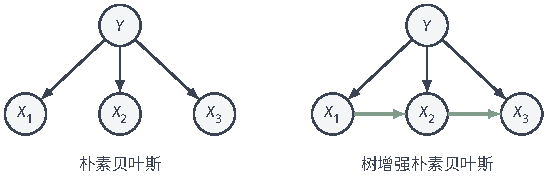
\includegraphics[width=92.650mm]{figures/06-probabilistic-graphical-models/04-models/tikz/pgm-static-directed-classifiers/figure.pdf}
  \caption{类别模型的两种属性结构。NB给定$Y$后各属性独立；TAN增加$X_1\to X_2\to X_3$，使右图的条件分布保留属性树上的依赖。训练时读入类别，预测时根据属性查询类别，观测状态随任务确定。}
  \label{fig:pgm-static-directed-classifiers}
\end{figure}

允许更大的父集，会增加需要估计的条件表。若属性$i$有$r_i$个状态，NB的自由参数为$(K-1)+K\sum_i(r_i-1)$；固定TAN属性树后，按父配置计数得到
\[
  (K-1)+K(r_r-1)
       +K\sum_{i\ne r}r_{t(i)}(r_i-1).
\]
两个类别和三个二值属性的自由参数由NB的$7$个增为TAN的$11$个，仍小于完整联合表所需参数，但新增父配置也需要数据支持。给定完整属性，两个模型枚举类别的评分均需$O(Kd)$次局部查询。二值TAN的对数评分还可含$x_i x_{t(i)}$项，因而能够表示属性间的交互。

TAN的学习包含参数估计与树选择两个层次。记定向后的属性树为$T$，固定它时，最大化
\begin{equation}
  \ell_T=\sum_{j=1}^n\left[
    \log\pi_{y_j}+\log p(x_{j,r}\mid y_j)
    +\sum_{i\ne r}\log p(x_{j,i}\mid y_j,x_{j,t(i)})\right].
  \label{eq:pgm-static-directed-tan-objective}
\end{equation}
每行条件表按类别与属性父值分组计数，再以该行总数归一化。树未知时，还需比较不同$T$各自达到的最大似然；下面把这个比较化成边权之和。选定树后重新按其父配置拟合条件表，便得到可用于类别预测的完整模型。

对于完整离散数据，可以选择使训练似然最大的属性树。先用经验分布$\widehat p$计算给定类别的条件互信息
\[
  \widehat I(X_i;X_j\mid Y)=
  \sum_{y,x_i,x_j}\widehat p(y,x_i,x_j)
  \log\frac{\widehat p(x_i,x_j\mid y)}
                 {\widehat p(x_i\mid y)\widehat p(x_j\mid y)}.
\]
求和只计算正频数项，零频数项以连续延拓取$0$。将候选树上的条件表分别拟合为最大似然表，其平均训练对数似然为
\begin{equation}
  \label{eq:pgm-static-directed-tan-score}
  -\widehat H(Y)-\sum_i\widehat H(X_i\mid Y)
  +\sum_{\{i,j\}\in E_{\mathrm{T}}}
       \widehat I(X_i;X_j\mid Y),
\end{equation}
这里$\widehat H$是经验熵，$E_{\mathrm T}$是属性树的无向边集。每个非根属性的条件熵可写为$H(X_i\mid Y,X_j)=H(X_i\mid Y)-I(X_i;X_j\mid Y)$，根仍贡献$H(X_r\mid Y)$；将各项相加，便得到式中的熵项与树边互信息。熵项不随树改变，因此以条件互信息为边权，求最大生成树并任取根定向即可。这个最大似然结论针对观测完整、无结构惩罚和自由条件表的设定，其他约束需重新分析得分。

若$r_i\le r$，直接统计全部属性对需$O(nd^2)$次计数更新，遍历条件表求边权需$O(Kd^2r^2)$操作，稠密最大生成树需$O(d^2)$时间。NB只统计单属性，计数为$O(nd)$。TAN增加这部分工作以拟合类内依赖，树结构仍限制可表达的高阶相互作用；数据稀疏时，新增条件表和不稳定的树边可能增加估计误差。Friedman等给出了TAN及其算法，结构学习的一般得分推导见第~\ref{chap:pgm-structure-learning}章\scite{pgm-static-directed-friedman1997}

\subsection{基于顺序条件的密度建模}
\label{sec:pgm-static-directed-autoregressive}

朴素贝叶斯需要一个已观测的类别节点来组织条件分布。若手头\emph{没有}类别标签、只想描述一条完整记录本身的联合分布，还有一个对任意联合分布都成立的通用办法：概率链式法则。它让我们人为给变量排一个顺序，然后把“整条记录的概率”写成第一个变量的边缘概率、给定第一个后第二个的条件概率、依此类推各项的连乘。这样做的好处是每一个因子都是一个归一化的条件分布，可以用功能很强的模型（如神经网络）逐个拟合，且无需引入任何潜变量、没有难以计算的积分；代价是要选定一个顺序，而且生成时只能沿该顺序逐个抽样。拟合观测的联合分布时，也可以依次为每个变量建立给定前面变量的条件分布。选定字段或像素的次序，把第$i$位以前的取值记为$\bm x_{<i}$。\term{自回归密度模型}（autoregressive density model）沿这个顺序计算条件概率，再相乘形成
\begin{equation}
  \label{eq:pgm-static-directed-ar}
  p_{\bm{\theta}}(\bm{x})
    =\prod_{i=1}^{d}p_{\bm{\theta}}(x_i\mid\bm{x}_{<i}).
\end{equation}
这种顺序规定预测前缀，例如表格字段排列或图像扫描顺序。第一个前缀$\bm x_{<1}$为空，因此第一项是边缘分布；各字段之间无需具有真实时间关系。

局部归一化保证式~\eqref{eq:pgm-static-directed-ar}的联合分布也归一化。离散变量先对$x_d$求和，最后一项变为$1$；依次消去$x_{d-1},\ldots,x_1$，最后留下$\sum_{x_1}p(x_1)=1$。连续变量使用非负可测、每个前缀下均归一化的条件密度，借助Tonelli定理依次积分，也得到总质量$1$。从某个联合分布恢复条件分布时，零概率前缀可补任意归一化条件分布，它与前缀零权重相乘后仍为零。归一化确定了概率合法性，拟合数据的质量还取决于所选条件函数。

链式法则允许任意联合分布沿任意变量排列分解。对二值变量使用完整条件表，仍需$1+2+\cdots+2^{d-1}=2^d-1$个自由参数。实际用有限宽度网络、有限感受野或高斯条件减少参数时，模型只保留这些局部函数可表达的分布。变量排列会改变待拟合的条件关系：一个方向的条件可能近似单峰，反向却可能出现多个峰，因此同样容量的函数在不同顺序下可产生不同误差。

消去例~\ref{ex:pgm-static-directed-binary}中的类别，得到两个读数的观测联合表
\[
  \begin{array}{ccccc}
    (x_1,x_2)&(0,0)&(0,1)&(1,0)&(1,1)\\
    p(x_1,x_2)&0.654&0.176&0.096&0.074
  \end{array}
\]
以$X_1$在前的顺序，将这张表改写为三个条件参数：
\[
  \begin{aligned}
    p(X_1=1)&=0.17,\\
    p(X_2=1\mid X_1=1)&=\frac{37}{85},\\
    p(X_2=1\mid X_1=0)&=\frac{88}{415}.
  \end{aligned}
\]
例如由$p(X_1=1)=0.17$和$p(X_2=1\mid X_1=1)=37/85$相乘，恢复$p(1,1)=0.074$。直接分解保留了整张读数联合表，用它能预测另一读数。若查询未观测工作状态$Y$，则还需要定义含$Y$的模型；观测表本身只给读数间的关系。

每个输出层需定义当前变量的完整条件分布。二值变量使用伯努利参数，有$r$个状态的变量使用softmax归一化概率；图像通道有$256$个离散值时，可以输出$256$项概率。连续条件可以输出均值$\mu_i(\bm x_{<i})$和正尺度$\sigma_i(\bm x_{<i})$来定义高斯密度，多峰条件则输出有限高斯混合的权重、均值和尺度。局部成分指示可被显式求和，因此混合参数化仍能计算这一条件似然。离散质量与连续密度使用不同的参考测度；将量化像素连续化时，还需给出量化区间积分或去量化方案。

完整训练记录提供每一位真实前缀，对这些条件分布的负对数似然求和，形成
\begin{equation}
  \label{eq:pgm-static-directed-ar-loss}
  L(\bm{\theta})=-\sum_{j=1}^{n}\sum_{i=1}^{d}
      \log p_{\bm{\theta}}
      (x_{j,i}\mid\bm{x}_{j,<i}).
\end{equation}
学习方法是把完整记录代入各条件函数，按式~\eqref{eq:pgm-static-directed-ar-loss}累加梯度，再更新共享参数。用小批量近似全数据梯度时，每个入选记录仍提供各位置的真实前缀。不同网络会采用逐步递推或同时前向计算，但共同优化的是这一个完整记录似然。额外的跨位置计算需要保持相同的读取约束，例如将全部输入汇总后广播到每个输出，会重新引入未来或当前目标信息。

生成记录时，条件所需的前缀尚待抽样。先取$X_1$，再据其结果取$X_2$，沿顺序继续，完成祖先采样。具有完整顺序依赖的标量模型要作$d$轮相继决策，不同记录可以批处理，同一记录则按前缀推进。缓存减少各轮重复计算，但前后状态的依赖仍保留。NB在类别给定后各属性独立，可并行抽样；TAN可按属性树的层次并行，生成顺序因此取决于具体父集。

自回归分解提供可计算的完整似然和顺序采样。观测的是前缀时，余下部分可按原条件分布续写；若第一位缺失、后面的多位已观测，计算第一位的后验可能需要汇总一批变量。选择模型时，应分别评估完整密度、祖先采样和任意条件补全的成本。第~\ref{chap:pgm-generative}章将沿用这条直接似然路线，与其他神经生成构造比较。

\subsubsection{NADE：复用逐步增长的前缀表示}
\label{sec:pgm-static-directed-nade-model}

用完整条件表实现自回归分解时，第$i$个条件分布要读取前面所有变量，参数表大小随$i$指数增长。换成神经网络拟合这些条件函数可以压缩参数量，但如果为每个位置$i$都各训练一个独立网络，又会有$d$个网络、彼此不共享，且无法利用“前$i$个变量的前缀”和“前$i+1$个变量的前缀”高度重叠这一事实。NADE的思路是让所有位置\emph{共用同一个网络}，并利用前缀只比上一步多一个变量的特点做增量计算：算出第$i$个条件所用的隐藏表示后，只需再加一项就能得到第$i+1$个条件的隐藏表示，而不必从头前向。逐前缀条件表的大小随维数增长。\term{神经自回归分布估计器}（neural autoregressive distribution estimator, NADE）让不同前缀共用网络参数，以限制需要保存的参数量。对二值观测，宽度为$h$的单隐藏层条件函数为
\begin{equation}
  \label{eq:pgm-static-directed-nade}
  \begin{aligned}
    \bm{a}_i&=\bm{c}+\sum_{j<i}\bm{W}_{:,j}x_j,&
    \bm{h}_i&=\operatorname{sigmoid}(\bm{a}_i),\\
    p(X_i=1\mid\bm{x}_{<i})
      &=\operatorname{sigmoid}
        (b_i+\bm{V}_{i,:}\bm{h}_i).
  \end{aligned}
\end{equation}
其中$\bm W\in\mathbb R^{h\times d}$、$\bm V\in\mathbb R^{d\times h}$，$\bm c,\bm b$为偏置，$\operatorname{sigmoid}(u)=(1+\exp(-u))^{-1}$。前缀从$i$延长到$i+1$时，用$\bm a_{i+1}=\bm a_i+\bm W_{:,i}x_i$增量更新，成本为$O(h)$；配合每位的输出计算，完整记录评价需$O(dh)$操作。$\bm h_i$由已知前缀确定，可直接计算，无需作为随机潜变量积分。这个前缀复用方式构成NADE计算似然的基础\scite{larochelle2011}

对式~\eqref{eq:pgm-static-directed-nade}输出的概率记$q_{j,i}$，NADE实际最小化的二值目标为
\[
 L_{\mathrm{NADE}}=-\sum_{j,i}
 [x_{j,i}\log q_{j,i}+(1-x_{j,i})\log(1-q_{j,i})].
\]
每轮沿前缀递推得到各$q_{j,i}$，将所有位置的误差信号反向传给共享的$\bm W,\bm V,\bm b,\bm c$，再作梯度更新。生成时把前一步抽得的值接入递推；有限隐藏宽度限制所能表示的条件函数，$O(dh)$计算量本身不保证拟合任意二值联合表。

\subsubsection{MADE：用掩码同时计算合法条件}
\label{sec:pgm-static-directed-made-model}

NADE要沿前缀一步步递推才能算完一条记录的似然，难以借助现代硬件一次性并行。于是产生一个诱人的想法：能不能让网络\emph{一次前向就同时输出}全部$d$个条件分布？难点在于自回归顺序要求“第$i$个输出只能看见前$i-1$个输入”，而普通全连接网络的每个输出能看见所有输入，会作弊地读到自己的当前值。MADE的解决办法非常直接：用一组固定的\emph{掩码}把违反顺序的连接权重强制置零，从结构上保证每个输出读取的恰好是它的合法前缀，从而在一次并行前向中算出全部条件。也可以同时计算各条件，但限制每个输出能读取的输入。\term{掩码自编码分布估计器}（masked autoencoder for distribution estimation, MADE）将违反自回归顺序的连接置零。给输入$j$次序号$j$、隐藏单元$u$次序号$m(u)$，仅保留输入边$j\le m(u)$与输出边$m(u)<i$。深层隐藏边的次序号非递减，输出端仍要求严格小于$i$，故每条输入到输出的路径都满足$j<i$。这样同时算出的第$i$个条件只使用合法前缀。

对单隐藏层二值输出，这些限制落实在权重矩阵上，模型结构可写成
\begin{equation}
  \bm h=\sigma((\bm W\odot\bm M_{\mathrm{in}})\bm x+\bm c),
  \qquad
  \bm q=\sigma((\bm V\odot\bm M_{\mathrm{out}})\bm h+\bm b),
  \label{eq:pgm-static-directed-made-structure}
\end{equation}
其中$\odot$为逐元素相乘，$\sigma$逐元素取sigmoid，$q_i$是第$i$个伯努利条件参数。训练使用与NADE相同的二值负对数似然，一次前向即可评价完整记录各位置；梯度只更新掩码允许的权重。生成时仍需先抽出第$i$位所依赖的前缀，再使用$q_i$，所以并行评价训练似然不等于并行生成整条记录。

图~\ref{fig:pgm-static-directed-mask}取三个输入和两个次序号分别为$1,2$的隐藏单元。以接收端为行、发送端为列，输入与输出掩码为
\[
  \bm{M}_{\mathrm{in}}=
  \begin{pmatrix}1&0&0\\1&1&0\end{pmatrix},\qquad
  \bm{M}_{\mathrm{out}}=
  \begin{pmatrix}0&0\\1&0\\1&1\end{pmatrix}.
\]
矩阵相乘得到$\left(\begin{smallmatrix}0&0&0\\1&0&0\\2&1&0\end{smallmatrix}\right)$，其非零项只在严格下三角，元素$2$计数两条合法路径。第一个条件输出仅用偏置，第三个输入只作为第三位似然的目标值，未进入任何条件参数。普通自编码器允许输出访问当前输入，可以通过复制完成重构。MADE结合前缀掩码与归一化条件输出，用各条件的负对数概率训练联合分布；这种似然目标需要由条件分布定义，普通重构误差则取决于另行选用的输出和损失\scite{pgm-static-directed-germain2015}

\begin{figure}[htbp]
  \centering
  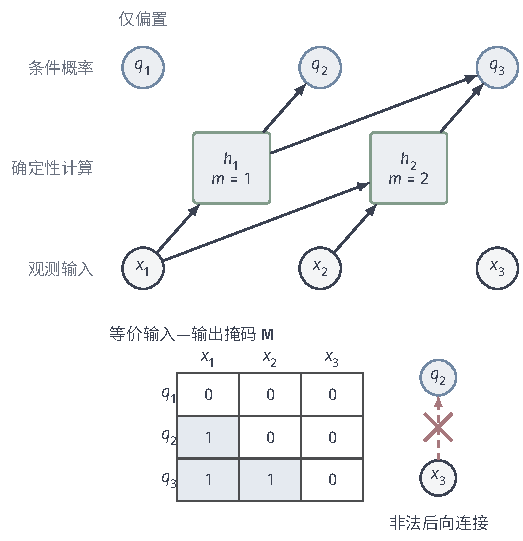
\includegraphics[width=88.554mm]{figures/06-probabilistic-graphical-models/04-models/tikz/pgm-static-directed-mask/figure.pdf}
  \caption{MADE掩码限定的条件依赖。隐藏方框进行确定性计算，输入与输出用圆框表示，$q_i=p(X_i=1\mid\bm x_{<i})$。下方输入—输出掩码中蓝色单元的1标出允许读取的前缀，右侧$x_3\to q_2$展示违反顺序的连接；各隐藏单元的次序号共同保证输出只能读取此前的输入。}
  \label{fig:pgm-static-directed-mask}
\end{figure}

\subsubsection{PixelCNN：把条件网络改为空间共享的掩码卷积}
\label{sec:pgm-static-directed-pixelcnn-model}

NADE、MADE都把输入当作一个没有空间结构的向量。但对图像而言，像素天然排布在二维网格上，同样的边缘、色块等局部图案会在图中不同位置反复出现；若为每个像素位置都单独保存一套连接权重，既浪费参数又无法利用这种“同一图案到处出现”的平移规律。卷积神经网络的优势正是让同一组卷积核在所有空间位置共享。于是只需把MADE的“掩码”思想搬到卷积上：按从上到下、从左到右的扫描顺序，让每个像素的条件网络只能读到它上方的行和同一行左侧的像素，就把空间权值共享与自回归的前缀约束结合起来。图像中相似的局部图案会出现在不同位置。为每个位置分别保存完整连接权重，没有利用这种重复；让相同卷积核在空间上复用，再屏蔽不合法的读取位置，就能把空间共享与前缀约束结合。

对图像，可用卷积共享不同位置的条件函数。\term{像素卷积自回归模型}（PixelCNN）按逐行扫描顺序，用掩码卷积读取当前像素上方和同行左侧的上下文。输入层排除当前目标值，后续层可读取当前位置已由合法前缀形成的隐藏表示。彩色图像还须规定像素内的通道顺序，例如红、绿、蓝，以使每个通道只访问此前通道。有限层数和卷积核限制可用感受野，模型虽归一化，却可能只利用部分前缀。原始论文同时介绍PixelCNN与PixelRNN，这里采用其中卷积掩码的依赖约束\scite{pgm-static-directed-oord2016}

具体到每通道$256$个离散值，网络在位置$i$输出得分$\bm f_{\bm\theta,i}$，条件结构与学习目标为
\begin{equation}
 \bm q_i=\operatorname{softmax}(\bm f_{\bm\theta,i}(\bm x_{<i})),
 \qquad L_{\mathrm{PixelCNN}}=-\sum_{j,i}\log q_{i,x_{j,i}}(\bm x_{j,<i}).
 \label{eq:pgm-static-directed-pixelcnn-objective}
\end{equation}
掩码卷积保证得分实际只读取允许的空间位置和此前通道，softmax保证各条件概率之和为$1$。每轮用真实图像前向计算所有条件，反向传播此目标并更新共享卷积核；生成则按同一像素和通道顺序抽样。NADE、MADE与PixelCNN因此共享自回归概率分解，改变的是前缀信息怎样计算、保存和复用。

\section{记录内共同变化的潜变量建模}
\label{sec:pgm-static-directed-latent}

聚类或压缩任务有时需要一个共同状态来解释多项读数。这个状态可以是每条记录选择的一种工作模式，也可以是连续变化的共同强度；本节先固定总体参数，研究一条记录内部的解释，跨记录的随机共享留到第~\ref{sec:pgm-static-directed-hierarchy-membership}节。为此可在观测外引入随机潜在坐标，再处理它们给定观测后的不确定性。\term{潜变量}（latent variable）指模型主动加入的未观测状态，漏记的字段则属于缺失数据，这一区别见第~\ref{sec:pgm-parameter-learning-definition}节。记潜在状态为$\bm z$，从它与观测的联合分布汇总得到
\begin{equation}
  \label{eq:pgm-static-directed-marginal}
  p_{\bm{\theta}}(\bm{x})=
  \begin{cases}
    \sum_{\bm{z}}p_{\bm{\theta}}(\bm{z})
          p_{\bm{\theta}}(\bm{x}\mid\bm{z}),
          &\text{离散潜变量},\\
    \int p_{\bm{\theta}}(\bm{z})
          p_{\bm{\theta}}(\bm{x}\mid\bm{z})\,d\bm{z},
          &\text{连续潜变量}.
  \end{cases}
\end{equation}
先验及各状态下的条件分布归一化，使观测分布的总质量为$1$。计算这个分布还要完成求和或积分，具体难度取决于潜变量和函数表示。仅由观测似然选择潜在解释时，也可能得到不同的等价分解；若要赋予它因果含义，需要更多依据。

\subsection{基于离散成分的混合建模}
\label{sec:pgm-static-directed-mixtures}

这一节转向本章的第二条主线：不再只在观测变量之间直接连边，而是为每条记录设想一个\emph{未观测的潜在状态}来解释它。先考虑最常见的情形——设备其实运行在若干离散的“工作模式”之一（如正常、过载、故障前兆），模式决定了这一整条记录的读数分布；但日志里并没有记录当前是哪种模式。把这个隐藏的模式选择记为$Z$，整条记录的分布就是“先按比例抽一种模式、再由该模式的分布生成读数”，对所有模式求和。这样一个“若干简单分布按比例混合”的模型就是有限混合模型；它同时解释了为什么单看两个读数会相关——它们只是共享了同一个隐藏模式。如果设备记录只含读数，工作状态可能由几个未标记的类别组成。\term{有限混合模型}（finite mixture model）先抽取成分，再用该成分的分布生成一条完整记录。成分$Z\in\{1,\ldots,K\}$具有权重$\pi_k\ge0$、$\sum_k\pi_k=1$，局部参数为$\bm\theta_k$，则
\begin{equation}
  \label{eq:pgm-static-directed-mixture}
  p(Z=k,\bm{x})=\pi_k p(\bm{x}\mid\bm{\theta}_k),
  \qquad
  p(\bm{x})=\sum_{k=1}^{K}\pi_kp(\bm{x}\mid\bm{\theta}_k).
\end{equation}
权重描述成分在总体中的比例，成分函数描述该状态下读数怎样变化。给定这些共享参数，每条记录独立抽取自己的$Z_j$，再生成观测。例~\ref{ex:pgm-static-directed-binary}若不记录类别，两个类内伯努利乘积就成为两成分混合；对类别求和后，仍得到前面的二元联合表。

有限混合的学习目标需要把没有记录的成分求和后再取对数：
\begin{equation}
 \max_{\bm\pi,\bm\theta_{1:K}}\;
 \ell_{\mathrm{mix}}=\sum_{j=1}^n\log\left[
    \sum_{k=1}^K\pi_kp(\bm x_j\mid\bm\theta_k)\right],
 \qquad \bm\pi\in\Delta^{K-1}.
 \label{eq:pgm-static-directed-mixture-objective}
\end{equation}
与NB的已知类别相比，每条记录现在不能直接归入一个计数组；其后验权重为$\pi_kp(\bm x_j\mid\bm\theta_k)/\sum_\ell\pi_\ell p(\bm x_j\mid\bm\theta_\ell)$。这些权重随参数变化，所以目标中的成分不再能像已标注类别那样分别优化。以下先说明混合解释相关性的机制，再用高斯成分展开EM。

共同成分怎样产生读数相关，可以把协方差分成类内和类间两部分。对具有有限二阶矩的两个属性，全协方差公式给出
\[
  \operatorname{Cov}(X_1,X_2)=
  \mathbb{E}\!\left[\operatorname{Cov}(X_1,X_2\mid Z)\right]
  +\operatorname{Cov}\!\left(
       \mathbb{E}[X_1\mid Z],\mathbb{E}[X_2\mid Z]\right).
\]
成分内部条件独立时，第一项为零，类间均值的共同变化仍可使第二项非零。前面二值读数的类间项为$0.1\times0.9\times(0.8-0.1)\times(0.7-0.2)=0.0315$，与联合表一致。若成分内部还有相关性，则保留第一项；有限混合本身并不规定成分内属性独立。

当读数是连续值时，最常用的成分分布是高斯分布；单个高斯只有一个峰、呈椭球状，无法描述“数据聚成好几团、每团中心和形状都不同”的情形，而把若干个高斯按比例混合，就能拼出多峰、任意形状的复杂分布。连续读数可以采用\term{高斯混合模型}（Gaussian mixture model, GMM）：$p(\bm x\mid Z=k)=\mathcal N(\bm x;\bm\mu_k,\bm\Sigma_k)$，各协方差正定。全协方差以$d(d+1)/2$个参数允许不同方向的相关和伸展；对角协方差以$d$个参数表示条件独立的属性；球形$\sigma_k^2\bm I$只估一个尺度。也可要求所有成分共享协方差，减少参数并让各成分具有同样形状。每个成分即使使用对角协方差，混合后的类间变化仍能形成非对角的总体协方差。

GMM将高斯成分代入式~\eqref{eq:pgm-static-directed-mixture-objective}，具体模型与目标是
\begin{equation}
 p(\bm x)=\sum_k\pi_k\mathcal N(\bm x;\bm\mu_k,\bm\Sigma_k),
 \qquad
 \ell_{\mathrm{GMM}}=\sum_j\log\sum_k\pi_k
          \mathcal N(\bm x_j;\bm\mu_k,\bm\Sigma_k).
 \label{eq:pgm-static-directed-gmm-objective}
\end{equation}
优化变量为权重、均值和满足选定约束的正定协方差；固定成分数$K$时，这才是EM要提高的观测目标。

固定参数后，用每个成分的先验权重乘该记录的密度，再对$K$项归一化，就得到\term{责任度}（responsibility），即记录属于各成分的后验概率。对高斯成分，第$t$轮参数下写成
\begin{equation}
  \label{eq:pgm-static-directed-responsibility}
  r_{j,k}^{(t)}=
  \frac{\pi_k^{(t)}
      \mathcal{N}(\bm{x}_j;\bm{\mu}_k^{(t)},\bm{\Sigma}_k^{(t)})}
       {\sum_{\ell=1}^{K}\pi_\ell^{(t)}
      \mathcal{N}(\bm{x}_j;\bm{\mu}_\ell^{(t)},\bm{\Sigma}_\ell^{(t)})}.
\end{equation}
对前面的二值混合，观测$(1,1)$属于异常成分的责任度同样是$28/37$。将类别作为潜在成分时，这些后验权重需要由当前参数推断，参数又要依据这些记录的归属来估计，两项计算因而交替进行。

EM在每轮先用旧参数计算式~\eqref{eq:pgm-static-directed-responsibility}中的责任度，再固定这些权重，优化新参数，通用推导见第~\ref{chap:pgm-parameter-learning}章。对高斯混合，需要最大化的期望完全数据对数似然为
\[
  \begin{aligned}
    Q={}&\sum_{j,k}r_{j,k}^{(t)}
       \left(\log\pi_k-\frac12\log|\bm{\Sigma}_k|\right)\\
       &-\frac12\sum_{j,k}r_{j,k}^{(t)}
         (\bm{x}_j-\bm{\mu}_k)^\top
          \bm{\Sigma}_k^{-1}(\bm{x}_j-\bm{\mu}_k)
       +\text{常数}.
  \end{aligned}
\]
在$\sum_k\pi_k=1$下对权重求驻点，得到加权样本比例；均值驻点为加权观测均值；将它代入协方差项，得到加权残差二阶矩。记有效样本数$N_k^{(t)}=\sum_jr_{j,k}^{(t)}$，当它为正且协方差更新保持正定时，三个更新为
\begin{equation}
  \label{eq:pgm-static-directed-gmm-em}
  \begin{aligned}
    \pi_k^{(t+1)}&=\frac{N_k^{(t)}}{n},\\
    \bm{\mu}_k^{(t+1)}
      &=\frac{\sum_jr_{j,k}^{(t)}\bm{x}_j}{N_k^{(t)}},\\
    \bm{\Sigma}_k^{(t+1)}
      &=\frac{1}{N_k^{(t)}}\sum_jr_{j,k}^{(t)}
       (\bm{x}_j-\bm{\mu}_k^{(t+1)})
       (\bm{x}_j-\bm{\mu}_k^{(t+1)})^\top.
  \end{aligned}
\end{equation}
协方差约束决定最后一步怎样汇总残差：对角模型取对角元素，球形模型取迹再除以$d$。这两种更新直接极大化各自的受约束目标，估计过程中始终使用相应的协方差形式。

\begin{example}[一轮可复核的高斯混合EM]
  \label{ex:pgm-static-directed-gmm-em}
  取一维人工记录$x_1=-1,x_2=1$，两个成分初始权重均为$1/2$、均值为$-1,1$、方差均为$1$。在$x_1$处，两成分的加权密度比为$1:\exp(-2)$，责任度矩阵为
  \[
    \bm{R}^{(0)}
      =\begin{pmatrix}a&1-a\\1-a&a\end{pmatrix},
    \qquad a=\frac{1}{1+\exp(-2)}\approx0.880797.
  \]
  两个成分的有效样本数各为$1$，所以新权重均仍为$1/2$；均值更新得到$\mu_1^{(1)}=1-2a\approx-0.761594$、$\mu_2^{(1)}=2a-1$。样本平方均为$1$，加权二阶矩也为$1$，减去新均值的平方得到
  \[
    (\sigma_1^2)^{(1)}=(\sigma_2^2)^{(1)}
      =1-(2a-1)^2\approx0.419974.
  \]
  责任度同时为两个成分保留正权重，两个新均值因此向中间移动；方差再围绕这些新均值估计。例子展示一次E步与M步的数值变化，尚未评价多轮优化的终点或新数据上的表现。
\end{example}

全协方差GMM先分解$K$个协方差矩阵，成本为$O(Kd^3)$，再计算$nK$个二次型及加权协方差统计，通常需$O(nKd^2)$操作。对角表示将统计成本降为$O(nKd)$。固定参数时，有限混合的似然与成分后验由可计算的$K$项得到，精确求和保持可行；学习还需求解非凸优化并选择成分数。计算责任度时可先求对数权重，减去最大值，再指数化归一化，以降低高维密度下溢的风险。

含至少两个成分、协方差无正下界的GMM存在以下退化路径：把某成分均值放到一个训练点，将协方差趋于零，该点的密度趋于无穷；其余成分继续覆盖其他记录，训练似然便可没有有限最大值。继续迭代少量样本的例子也会面临这种边界。协方差特征值下界、适当先验或受约束估计可限制这类路径，但相应地改变学习目标；手工重置成分还需另行检查单调性。实际可从分散记录或聚类中心多次初始化，比较所得解；有效样本数近零时，按预定规则处理空成分。选择成分数时，再结合留出似然和应用任务，评估新增成分在训练数据以外的收益。

参数还具有\term{标签交换}（label switching）对称性。对任意两个成分，同时交换权重、均值和协方差，式~\eqref{eq:pgm-static-directed-mixture}给出的观测分布完全相同，编号本身无法由数据确定。置换得到的是同一预测分布的命名变化，另一个局部极值则可能给出不同预测。某些混合族在条件满足时可除置换外识别，但这个两成分、两二值属性例子有$5$个自由参数，观测表仅有$3$个自由度，通常还存在其他非唯一分解。解释成分或汇总对称后验时，应保留这种差异：不同编号的参数直接平均，可能破坏原本有用的预测表示。Murphy的教材讨论混合分布及其估计\scite{pgm-murphy2012}

\subsection{基于连续因子的观测建模}
\label{sec:pgm-static-directed-linear-gaussian}

离散混合假设每条记录\emph{恰好属于}一个隐藏类别，是“非此即彼”的归属。但很多共同原因本身是连续变化的：负载、振动强度、环境温度都可强可弱，一条记录往往同时受到\emph{好几个}强弱不同的共同因素影响，而不是只选其中一个。这时更自然的模型是用几个连续的潜在“因子”线性叠加来解释观测，剩下解释不了的部分归于每个传感器独有的噪声；这就是因子分析。它把每个观测读数理解成“少数共同因子的加权组合＋自身噪声”，从而用降维后的连续坐标刻画记录之间的共同变化。离散混合让一条记录选择一种模式；连续因子模型则允许同一条记录同时带有多个强弱不同的共同因素。两者都通过潜变量解释观测关系，但潜在状态的含义、汇总运算和后验形式不同。

\subsubsection{因子分析：把相关性分成共同因子与独有噪声}
\label{sec:pgm-static-directed-fa-model}

多个读数也可能随连续的负载或振动强度共同变化。用$q<d$个潜在坐标表示这部分变化，剩余各维由独有噪声解释，就得到\term{因子分析}（factor analysis, FA）的线性高斯模型
\begin{equation}
  \label{eq:pgm-static-directed-fa}
  \begin{aligned}
    \bm{Z}&\sim\mathcal{N}(\bm{0},\bm{I}_q),\\
    \bm{X}&=\bm{\mu}+\bm{W}\bm{Z}+\bm{\varepsilon},\\
    \bm{\varepsilon}&\sim\mathcal{N}(\bm{0},\bm{\Psi}),\qquad
    \bm{\Psi}=\operatorname{diag}(\psi_1,\ldots,\psi_d),
    \quad\psi_i>0.
  \end{aligned}
\end{equation}
潜变量$\bm Z$与噪声$\bm\varepsilon$独立，$\bm\mu\in\mathbb R^d$是观测均值，载荷$\bm W\in\mathbb R^{d\times q}$的每列说明一个潜在坐标怎样同时影响各读数。给定所有潜在坐标，均值中的各因子贡献相加，观测只剩对角协方差的独立噪声。

线性变换保留高斯形式，独立的潜在贡献与噪声又使协方差相加，因此积分消去潜变量后得到
\begin{equation}
  \label{eq:pgm-static-directed-fa-marginal}
  \bm{X}\sim\mathcal{N}(\bm{\mu},\bm{C}),\qquad
  \bm{C}=\bm{W}\bm{W}^{\top}+\bm{\Psi}.
\end{equation}
共同变化$\bm W\bm W^\top$的秩至多为$q$，对角$\bm\Psi$记录各传感器独有的噪声。这个约束规定了相关性必须由共同因子解释。若让噪声协方差完全自由，噪声也能吸收观测相关，因子与噪声间的分配就更加不确定。

模型结构确定后，学习希望让这些高斯边缘分布解释完整训练记录。令$\bm C=\bm W\bm W^\top+\bm\Psi$，FA的观测目标为
\begin{equation}
 \ell_{\mathrm{FA}}(\bm\mu,\bm W,\bm\Psi)
   =\sum_j\log\mathcal N(\bm x_j;\bm\mu,\bm C),
 \qquad \bm\Psi\text{为正对角矩阵}.
 \label{eq:pgm-static-directed-fa-objective}
\end{equation}
对固定正定$\bm C$，对均值求导得到$\widehat{\bm\mu}=\overline{\bm x}$。将均值固定为这个样本均值，记$\bm y_j=\bm x_j-\overline{\bm x}$、$\bm S_x=n^{-1}\sum_j\bm y_j\bm y_j^\top$，去掉与$\bm W,\bm\Psi$无关的常数后，等价于最小化
\[
 \frac n2\left[\log|\bm C|+
                  \operatorname{tr}(\bm C^{-1}\bm S_x)\right].
\]
第一项惩罚无界扩张协方差，第二项评价观测偏差相对于模型协方差的大小；二者共同决定拟合，不能只压低残差。直接优化这个目标是一条路线，EM则先计算每条记录潜在因子的后验矩，再用这些矩更新载荷和噪声。

给定观测，需要估计潜在坐标及其误差。令中心化读数$\bm y=\bm x-\bm\mu$，后验二次项系数$\bm M=\bm I_q+\bm W^\top\bm\Psi^{-1}\bm W$，先验与条件密度相乘后的$\bm z$项为
\[
  \begin{aligned}
    -2\log p(\bm{z}\mid\bm{x})
      &=\bm{z}^{\top}\bm{z}
       +(\bm{y}-\bm{W}\bm{z})^{\top}
          \bm{\Psi}^{-1}(\bm{y}-\bm{W}\bm{z})
       +\text{常数}\\
      &=\bm{z}^{\top}\bm{M}\bm{z}
       -2\bm{z}^{\top}\bm{W}^{\top}\bm{\Psi}^{-1}\bm{y}
       +\text{常数}.
  \end{aligned}
\]
正定噪声使$\bm M$正定。对上式配方，写成$(\bm z-\bm m)^\top\bm M(\bm z-\bm m)+\text{常数}$，读取高斯中心和精度，得到
\begin{equation}
  \label{eq:pgm-static-directed-fa-posterior}
  \begin{aligned}
    p(\bm{z}\mid\bm{x})&=\mathcal{N}(\bm{z};\bm{m},\bm{S}),\\
    \bm{S}&=\bm{M}^{-1},\qquad
    \bm{m}=\bm{S}\bm{W}^{\top}\bm{\Psi}^{-1}
                  (\bm{x}-\bm{\mu}).
  \end{aligned}
\end{equation}
后验均值表示给定读数的潜在坐标估计，后验协方差量化剩余不确定性。权重$\bm\Psi^{-1}$让噪声较小的测量在相同载荷下贡献较多精度，先验则提供单位精度，使证据较弱的坐标向零收缩。在固定参数、完整观测的条件下，协方差由$\bm M$决定，读数数值只改变后验均值。

对独立同分布的完整记录，已将FA的均值固定为样本均值，以下以$\bm y_j=\bm x_j-\overline{\bm x}$中心化。E步用旧参数和式~\eqref{eq:pgm-static-directed-fa-posterior}得到$\bm m_j,\bm S$，并形成二阶矩$\bm T_j=\bm S+\bm m_j\bm m_j^\top=\mathbb E[\bm Z_j\bm Z_j^\top\mid\bm x_j]$。M步对期望加权残差目标中的载荷求导，得到
\[
  \bm{W}^{(t+1)}\sum_j\bm{T}_j
     =\sum_j\bm{y}_j\bm{m}_j^\top.
\]
这个矩阵方程右乘$\left(\sum_j\bm T_j\right)^{-1}$，可写出载荷更新。每项$\bm T_j$都包含正定$\bm S$，所以在正噪声与有限参数的当前迭代下，系数矩阵可逆。实际计算可直接求解矩阵方程，避免显式构造逆矩阵。

估计噪声时，还需把潜在坐标的后验方差计入残差。用$\bm W_+=\bm W^{(t+1)}$表示新载荷，期望残差协方差为
\begin{equation}
  \label{eq:pgm-static-directed-fa-residual}
  \begin{aligned}
    \bm{R}=\frac1n\sum_j\bigl[
      &(\bm{y}_j-\bm{W}_{+}\bm{m}_j)
       (\bm{y}_j-\bm{W}_{+}\bm{m}_j)^\top\\
      &+\bm{W}_{+}\bm{S}\bm{W}_{+}^\top
    \bigr].
  \end{aligned}
\end{equation}
FA逐维取$\psi_i^{(t+1)}=\bm R_{i,i}$。残差的第二项将潜变量后验方差映射到观测空间；若省掉它，就少计了一项半正定协方差贡献，噪声估计可能偏小。解析E步和这项M步共同构成模型的EM迭代，单调性条件见第~\ref{chap:pgm-parameter-learning}章。噪声趋于零时，还需检查边界解和数值条件。

\subsubsection{概率主成分分析及线性因子模型的查询}
\label{sec:pgm-static-directed-ppca-model}

将残余噪声约束为$\bm\Psi=\sigma^2\bm I_d$，得到\term{概率主成分分析}（probabilistic principal component analysis, PPCA）。FA分别估计每维噪声，PPCA要求在当前坐标单位下各方向噪声同方差。改变特征单位会改变后一假设的含义，因此尺度选择需要与噪声模型一致。两种模型都提供潜在表示，同时给出这些坐标的后验不确定性。

PPCA沿用式~\eqref{eq:pgm-static-directed-fa-objective}，但把候选协方差限制为$\bm C=\bm W\bm W^\top+\sigma^2\bm I_d$、$\sigma^2>0$。它仍估计样本均值，在同一协方差目标下只优化$\bm W$和共同噪声方差。EM的E步及载荷更新不变，只需在相应矩阵中代入各向同性噪声；噪声M步变为$(\sigma^2)^{(t+1)}=\operatorname{tr}(\bm R)/d$。这一步把各维期望残差平均，正是共同方差约束下的极大化结果。

PPCA的最大似然载荷也可由样本协方差求得。令$\bm S_x=n^{-1}\sum_j\bm y_j\bm y_j^\top$，特征值按$\lambda_1\ge\cdots\ge\lambda_d$排列，前$q$个特征向量组成$\bm U_q$。当其余特征值的平均值为正时，解为
\begin{equation}
  \label{eq:pgm-static-directed-ppca-ml}
  \begin{aligned}
    \widehat{\sigma}^2
      &=\frac{1}{d-q}\sum_{i=q+1}^{d}\lambda_i,\\
    \widehat{\bm{W}}
      &=\bm{U}_q
       (\bm{\Lambda}_q-\widehat{\sigma}^2\bm{I}_q)^{1/2}
       \bm{R}_0,\qquad
       \bm{R}_0\bm{R}_0^\top=\bm{I}_q,
  \end{aligned}
\end{equation}
其中$\bm\Lambda_q=\operatorname{diag}(\lambda_1,\ldots,\lambda_q)$。负对数似然的协方差项为$\log|\bm C|+\operatorname{tr}(\bm C^{-1}\bm S_x)$：固定模型特征值，迹的重排不等式要求把最大的模型方差与最大的观测方差对齐。此后每个自由方向贡献$\log c_i+\lambda_i/c_i$，在$c_i=\lambda_i$处最小；其余$d-q$维共用$\sigma^2$，对这部分总和求导就得到剩余特征值的平均数。保留方向的重根会产生主轴选择的不唯一性；噪声估计为零则到达奇异边界，正定高斯密度的公式需重新处理。Tipping与Bishop给出了这个似然解及EM方法\scite{tipping1999}

为比较概率表示与几何投影，在保留的$\lambda_i>\widehat\sigma^2$方向，将潜变量后验均值映回观测空间，得到
\[
  \widehat{\bm{W}}\bm{m}
    =\bm{U}_q\operatorname{diag}
       \left(1-\frac{\widehat{\sigma}^2}{\lambda_i}\right)_{i=1}^{q}
       \bm{U}_q^\top\bm{y}.
\]
PCA把读数正交投影到所选子空间，PPCA还按信噪比缩小其中的坐标。固定满列秩载荷并令$\sigma^2$趋于零，均值重构的极限才是列空间上的正交投影；零噪声处的模型分布位于低维支持，已不是全维正密度。这样可由有噪声的后验重构联系降维几何，同时保留噪声条件的作用。

取人工样本协方差的特征值$5,2,1$，只保留一个因子。PPCA估计$\widehat\sigma^2=(2+1)/2=1.5$，可选$\widehat{\bm W}=\sqrt{3.5}\bm u_1$，得到模型协方差特征值$5,1.5,1.5$。后两方向被共同噪声方差合并，潜变量后验方差为$(1+3.5/1.5)^{-1}=0.3$。均值重构为$0.7\bm u_1\bm u_1^\top\bm y$，显示相对于PCA投影的收缩幅度。

某些传感器未读取时，潜在状态的不确定性随证据减少而变化。记观测索引$O\subseteq\{1,\ldots,d\}$，缺失索引为$U$，在式~\eqref{eq:pgm-static-directed-fa-posterior}中只保留$\bm W_{O,:}$、$\bm\Psi_{O,O}$及$\bm x_O-\bm\mu_O$，得到$\bm m_O,\bm S_O$。再利用独立残余噪声，把这些后验矩传播到缺失读数，得到
\begin{equation}
  \label{eq:pgm-static-directed-fa-missing}
  \begin{aligned}
    \mathbb{E}[\bm{X}_U\mid\bm{x}_O]
      &=\bm{\mu}_U+\bm{W}_{U,:}\bm{m}_O,\\
    \operatorname{Cov}(\bm{X}_U\mid\bm{x}_O)
      &=\bm{\Psi}_{U,U}
        +\bm{W}_{U,:}\bm{S}_O\bm{W}_{U,:}^\top.
  \end{aligned}
\end{equation}
缺失读数的预测方差包括自身噪声$\bm\Psi_{U,U}$，以及共同因子尚不确定带来的$\bm W_{U,:}\bm S_O\bm W_{U,:}^\top$。填入条件均值只保存一个估计值；后续使用填补数据时，还需处理这两项预测误差。

\begin{example}[两台传感器对一个连续因子的测量]
  \label{ex:pgm-static-directed-fa-missing}
  取$q=1,d=2$、$\bm\mu=\bm{0}$、$\bm W=(1,2)^\top$和$\bm\Psi=\operatorname{diag}(1,4)$作为人工模型，观测协方差为
  \[
    \bm{C}=\begin{pmatrix}2&2\\2&8\end{pmatrix}.
  \]
  完整读数$(2,4)$给出后验精度$1+1^2/1+2^2/4=3$、线性项$1\times2/1+2\times4/4=4$，所以$Z\mid(2,4)\sim\mathcal N(4/3,1/3)$。

  只保留$X_1=2$，后验精度变为$2$，得到$Z\mid X_1=2\sim\mathcal N(1,1/2)$。第二读数的预测均值为$2\times1=2$，方差为$4+2^2/2=6$。在观测空间直接条件化，也得到均值$(2/2)\times2=2$和方差$8-2^2/2=6$，两条计算路线一致。
\end{example}

载荷及坐标存在\term{旋转不唯一性}（rotational non-identifiability）。任意正交$\bm R_0$下，将载荷变为$\bm W\bm R_0$、坐标变为$\bm R_0^\top\bm Z$，潜在先验和观测协方差都保持原样。数据似然因而只约束相应分布，一维时也无法确定因子符号。为把某个因子命名为物理强度，需要额外约束、实验或领域信息；FA还可能有载荷和独有噪声的其他分解歧义。

对完整记录和对角噪声，形成$\bm M$需$O(dq^2)$操作，分解它需$O(q^3)$；复用相关矩阵后，各记录后验均值的计算为$O(dq)$。用Woodbury恒等式和行列式引理，也能以潜在空间矩阵计算观测似然：
\[
  \bm{C}^{-1}=\bm{\Psi}^{-1}
    -\bm{\Psi}^{-1}\bm{W}\bm{S}\bm{W}^{\top}\bm{\Psi}^{-1},
  \qquad |\bm{C}|=|\bm{\Psi}|\,|\bm{M}|,
\]
这两个恒等式使密度评价可避开$d\times d$稠密分解。完整数据的一轮EM通常为$O(ndq+nq^2+dq^2+q^3)$，噪声更新只计算残差协方差的对角元素。相同缺失模式可共用后验精度，不同模式需分别形成矩阵。缺失数据的E步还要计算缺失量的条件矩，均值更新也要利用这些矩。只对已观测数据最大化似然的适用条件，需结合第~\ref{chap:pgm-parameter-learning}章的缺失机制与可忽略性分析。

\section{跨记录与分组观测的共享建模}
\label{sec:pgm-static-directed-hierarchy-membership}

前两节的模型都把$n$条记录看作来自同一个总体、彼此独立同分布。但现实数据常常是\emph{分组}的：记录来自不同工厂、不同用户、不同文档。同型号设备在不同工厂工作，各厂参数可能相似又各有偏差；同一文档也可能同时包含设备和维修等多个主题。这类任务需要进一步规定哪些未知量跨记录共享、哪些选择在记录内部变化。本节分别考察组参数来自共同总体、组内逐项使用共享成分，以及随机成分库怎样跨记录或跨组复用。这些机制可组合；共享一个固定参数并不等于已经为组间异质性建立了随机层次。

\subsection{组参数的共享与部分汇聚}
\label{sec:pgm-static-directed-partial-pooling}

设有的工厂仅提供两条测量，另一些工厂提供几十条。各厂独立估计能够保留差异，却使小样本厂的均值波动很大；完全合并则要求所有工厂共用均值。让每厂有自己的均值，同时把这些均值放进一个共同总体，便在两种极端之间留下可估计的共享程度。

在“每组各估一套参数”和“所有组合并成一套参数”这两个极端之间，存在一个自然的折中：让每组拥有自己的参数，但规定这些组参数都\emph{抽自同一个共享的上层分布}。于是数据多的组主要由自己的数据决定，数据少的组则被向上层中心“拉一把”，各组还能通过这个共同上层互相借力。\term{层次模型}（hierarchical model）让各组参数来自一个共享的上层分布，以联系组间规律。\term{板表示法}（plate notation）用带索引的框标出节点与边的重复范围：组板内、样本板外的节点每组复制一次，两板内部的节点在每组的每个样本复制一次。给定索引后展开这些副本及连接，就得到联合分解的完整图。板框表示重复组织，概率因子仍由展开后的节点和父集决定。

例如组$g$的测量服从$X_{g,j}\mid\mu_g\sim\mathcal N(\mu_g,\sigma^2)$，组均值来自$\mu_g\sim\mathcal N(m_0,\tau^2)$。给定组均值，所有测量独立；给定上层参数，各组均值也独立。取已知$m_0$及正数$\sigma^2,\tau^2$，组内$n_g$条记录的均值为$\overline x_g$，配方得到
\begin{equation}
  \label{eq:pgm-static-directed-pooling}
  \begin{aligned}
    \mathbb{E}[\mu_g\mid\bm{x}_g]
      &=a_g\overline x_g+(1-a_g)m_0,\\
    a_g&=\frac{n_g\tau^2}{\sigma^2+n_g\tau^2},\\
    \operatorname{Var}(\mu_g\mid\bm{x}_g)
      &=\left(\tau^{-2}+n_g\sigma^{-2}\right)^{-1}.
  \end{aligned}
\end{equation}
权重$a_g$随组内样本数增加而增大，随测量噪声增加而减小，后验均值在本组平均值与共享中心$m_0$之间变化。这正是\term{部分汇聚}（partial pooling）的含义：既不像“完全不汇聚”那样让小样本组各自为战、估计剧烈波动，也不像“完全汇聚”那样强行抹平所有组的差异，而是在保留组间差异的同时，用共同分布把数据较少的组向中心收缩，收缩多少由该组数据量自动决定。取人工参数$m_0=0,\tau^2=1,\sigma^2=4,\overline x_g=3$，两条测量得到后验均值$1$，二十条测量得到$2.5$。两种收缩程度来自先验与测量精度的相对比例。

这一组层与样本层结构也直接给出观测分布。令$\bm x_g$收集工厂$g$的$n_g$条记录，$\bm1$为$n_g$维全1向量，积分掉$\mu_g$得到
\[
 \bm X_g\sim\mathcal N(m_0\bm1,
       \sigma^2\bm I_{n_g}+\tau^2\bm1\bm1^\top).
\]
组内不同记录因共同均值而具有协方差$\tau^2$。固定超参数时，各组之间仍独立，这与把全组数据当作独立测量的似然不同。

若共享参数需要从数据估计，经验贝叶斯的明确目标是
\begin{equation}
 \ell_{\mathrm{EB}}(m_0,\tau^2,\sigma^2)
 =\sum_g\log\int\mathcal N(\mu_g;m_0,\tau^2)
                \prod_j\mathcal N(x_{g,j};\mu_g,\sigma^2)\,d\mu_g.
 \label{eq:pgm-static-directed-pooling-objective}
\end{equation}
这里优化$m_0$及待估的正方差；若$\sigma^2$已知，就固定它。EM用旧超参数和式~\eqref{eq:pgm-static-directed-pooling}得到组后验均值$m_g$与方差$s_g^2$，再更新
\[
 \begin{aligned}
 m_0^+&=G^{-1}\sum_gm_g, &
 (\tau^2)^+&=G^{-1}\sum_g[(m_g-m_0^+)^2+s_g^2],\\
 (\sigma^2)^+&=\frac{\sum_{g,j}[(x_{g,j}-m_g)^2+s_g^2]}{\sum_g n_g}.
 \end{aligned}
\]
$G$是组数，加号表示本轮的新参数；每个方差更新同时包括均值残差和后验不确定性。重新计算组后验后继续迭代，检查边缘似然变化、方差边界和停止容差，不能用一次组均值平均替代整个学习过程。

式~\eqref{eq:pgm-static-directed-pooling}中的共享分布固定已知时，本组后验只读取本组数据；其他组的新增记录不会改变它。若用全部组估计$m_0,\tau^2$，或为它们设先验再联合推断，各组便通过未知共享量交换信息。例如将$\mu_g$作为潜在组参数进行EM，E步求其后验矩，共同$\tau^2$下的M步将$m_0$更新为各组$\mathbb E[\mu_g\mid\mathcal D]$的平均。完全贝叶斯方法继续积分共享参数的不确定性。组级分布假设需要与组间规律相符，否则向同一中心收缩会引入偏差。

完全贝叶斯分析为$\bm h=(m_0,\tau^2,\sigma^2)$指定适当先验，目标变为
\[
 p(\bm h,\mu_{1:G}\mid\mathcal D)
 \propto p(\bm h)\prod_g p(\mu_g\mid\bm h)
                         \prod_jp(x_{g,j}\mid\mu_g,\bm h).
\]
可以交替更新组均值与共享参数的条件后验，不能解析的部分使用前文的采样或变分计算。固定超参数时，已有组下一条记录的预测为$\mathcal N(m_g,\sigma^2+s_g^2)$；尚无数据的新组则为$\mathcal N(m_0,\sigma^2+\tau^2)$。完全贝叶斯预测还要对$\bm h$的后验积分，经验贝叶斯则把拟合的$\bm h$直接代入，两种输出对共享参数不确定性的处理不同。

\subsection{组内逐项分配与混合成员}
\label{sec:pgm-static-directed-mixed-membership}

有限混合模型给\emph{整条记录}只分配一个隐藏类别——一台设备要么正常、要么异常，一篇文档要么属于这个主题、要么属于那个主题。但很多对象天然是“多种成分按比例混合”的：一篇文档往往同时讨论设备、维修、安全等多个主题，不同段落甚至不同词语各自侧重不同主题。于是更细的做法是把分配单位从“整条记录”下沉到“记录里的每一项”：整组持有一个关于各成分的\emph{比例}，组内每个观测再按这个比例各自挑选成分。同一组中每个局部观测还可以选择自己的成分，这种结构称为\term{混合成员}（mixed membership）。一篇同时讨论设备和维修的文档，每个词分别选择主题，文档的主题比例控制这些选择；主题本身是词概率分布，其语义名称需由数据和应用解释。设文档$g=1,\ldots,G$有$N_g$个词，词表大小为$v$，词编号为$X_{g,j}\in\{1,\ldots,v\}$。主题词概率向量$\bm\beta_k$与文档主题比例$\bm\pi_g$各自非负、分量和为$1$。

\subsubsection{pLSA：每篇文档拥有固定比例，每个词选择主题}
\label{sec:pgm-static-directed-plsa-model}

先看混合成员思想最朴素的实现：不给文档主题比例的来源建模，而是把每篇训练文档的比例直接当作一组需要估计的\emph{自由参数}。有限混合为整条记录只抽一个成分，不能直接描述一篇文档在不同词位置使用不同主题的过程。让文档持有一组比例、每个词重新选择主题，就能保留文档内的多主题构成。

\term{概率潜在语义分析}（probabilistic latent semantic analysis, pLSA）为每篇训练文档估计一个固定比例$\bm\pi_g$。给定文档编号，词位置$j$先从$\operatorname{Categorical}(\bm\pi_g)$抽主题$Z_{g,j}$，再从相应$\bm\beta_{Z_{g,j}}$抽词，得到
\begin{equation}
  \label{eq:pgm-static-directed-plsa}
  p(\bm{x}_g\mid\bm{\pi}_g,\bm{\beta}_{1:K})
    =\prod_{j=1}^{N_g}
       \sum_{k=1}^{K}\pi_{g,k}\beta_{k,x_{g,j}}.
\end{equation}
$\operatorname{Categorical}$给出类别抽样概率，$\beta_{k,a}$是主题$k$产生词$a$的概率。给定固定比例与主题参数，不同词各有自己的主题后验，权重正比于$\pi_{g,k}\beta_{k,x_{g,j}}$，各位置的后验独立。EM用这些责任度更新文档比例为平均主题责任度，再按全语料加权词频更新主题分布。相同词可合并为词频以复用计算。Hofmann介绍了pLSA的混合分解与EM估计\scite{pgm-static-directed-hofmann1999}

pLSA的目标与学习步骤可以写成一组可执行的更新。最大化
\begin{equation}
 \ell_{\mathrm{pLSA}}=\sum_{g,j}\log\sum_k\pi_{g,k}\beta_{k,x_{g,j}},
 \qquad \bm\pi_g\in\Delta^{K-1},\quad\bm\beta_k\in\Delta^{v-1}.
 \label{eq:pgm-static-directed-plsa-objective}
\end{equation}
从正的归一化参数开始，E步对每个词归一化当前主题权重；M步分别汇总文档内的主题计数与全语料的主题词计数：
\[
 \begin{aligned}
 r_{g,j,k}&=\frac{\pi_{g,k}\beta_{k,x_{g,j}}}
                   {\sum_\ell\pi_{g,\ell}\beta_{\ell,x_{g,j}}},\\
 \pi_{g,k}^+&=\frac1{N_g}\sum_jr_{g,j,k},\qquad
 \beta_{k,a}^+=\frac{\sum_{g,j}r_{g,j,k}\mathbb I\{x_{g,j}=a\}}
                         {\sum_{g,j}r_{g,j,k}}.
 \end{aligned}
\]
这里要求$N_g>0$且被更新主题的总责任度为正，分母为零时需预先约定保留、平滑或重置规则。用新参数重算责任度，迭代到目标变化足够小或预算用尽；该停止条件不保证全局最优。

pLSA的文档比例一共包含$G(K-1)$个自由参数，随训练文档数增长。遇到新文档，可固定已学主题，再由新词拟合一组比例，称为折入估计。这个步骤扩展了参数表，但原模型没有描述新比例的随机来源；需要组级生成时，就要进一步为比例定义分布。

\subsubsection{LDA的比例生成与主题学习}
\label{sec:pgm-static-directed-lda-model}

pLSA有一个明显的缺口：它的主题比例是逐篇文档硬估出来的参数，参数数量随文档数线性增长，模型并没有描述“一篇新文档的比例从哪里来”，因此无法天然地为没见过的文档生成概率。要补上这一环，就得把文档比例本身也提升为一个\emph{随机变量}，给它一个先验分布（通常用Dirichlet分布）；新文档先从这个先验抽出比例，再依据实际看到的词把比例的后验收缩。新文档没有已拟合的比例表项。若希望模型在读取新词之前就能生成一篇文档，需要给比例本身安排随机来源，再用新词修正这份不确定性。

\term{潜在狄利克雷分配}（latent Dirichlet allocation, LDA）为每篇文档的比例设置先验，使新文档也有相同的生成步骤。
比例先验采用Dirichlet分布。
记$\bm\pi_g\sim\operatorname{Dirichlet}(\bm\alpha)$，各$\alpha_k>0$，总质量为$\alpha_0=\sum_k\alpha_k$；其密度在概率单纯形内部正比于$\prod_k\pi_{g,k}^{\alpha_k-1}$，均值为$\alpha_k/\alpha_0$。它为比例向量提供共同中心及不同的分散程度，可参考\BookChapterRef{chap:random-variables}{卷2《数学准备：概率、因果与决策》的“随机变量与概率基础”章}。
先抽文档比例，再逐词抽取主题和词值。
给定主题词分布，其联合分布及对比例、主题汇总后的观测分布为
\begin{equation}
  \label{eq:pgm-static-directed-lda}
  \begin{aligned}
    p(\bm{\pi}_g,\bm{z}_g,\bm{x}_g\mid
          \bm{\alpha},\bm{\beta}_{1:K})
      &=p(\bm{\pi}_g\mid\bm{\alpha})
         \prod_j\pi_{g,z_{g,j}}\beta_{z_{g,j},x_{g,j}},\\
    p(\bm{x}_g\mid\bm{\alpha},\bm{\beta}_{1:K})
      &=\int p(\bm{\pi}_g\mid\bm{\alpha})
          \prod_j\left(\sum_k
              \pi_{g,k}\beta_{k,x_{g,j}}\right)d\bm{\pi}_g.
  \end{aligned}
\end{equation}
这里固定文档长度，只建模其中的词。各文档共用$\bm\alpha$和主题分布，新文档的比例按先验产生，再根据词进行后验推断。于是模型给出了固定长度下的新文档生成分布，词序或语法还需别的结构描述。

给定$\bm\pi_g$，各位置的词独立同分布；积分掉这个共同随机比例后，位置间一般相关，但任意词序排列仍有相同概率，即词袋的可交换性。若把样本改为词计数向量，还需乘相应的多项式计数系数。LDA由此加入了pLSA所缺的文档级比例先验，同时需要处理比例积分；原始论文给出模型、变分推断和经验贝叶斯学习\scite{blei2003}

\begin{example}[固定比例、随机比例与整组单一主题]
  \label{ex:pgm-static-directed-lda-two-words}
  用两词词表$\{a,b\}$及主题$\bm\beta_1=(0.8,0.2)$、$\bm\beta_2=(0.2,0.8)$比较三种共享方式。取LDA先验$\bm\alpha=(1,1)$，则$\pi_{g,1}=u$均匀分布于$[0,1]$，$\pi_{g,2}=1-u$。给定$u$，词$a$的概率为$0.2+0.6u$，边缘为$1/2$；两词均为$a$时需要对同一个$u$积分，得到
  \[
    p(a,a)=\int_0^1(0.2+0.6u)^2\,du
      =0.04+0.12+0.12=0.28.
  \]
  固定比例$(1/2,1/2)$时，式~\eqref{eq:pgm-static-directed-plsa}给出$0.5^2=0.25$；整篇仅选一个主题时，概率为$(0.8^2+0.2^2)/2=0.34$。三种模型的单词边缘均为$1/2$，但共享方式导致双词联合概率不同。

  在LDA中，四种主题配置$(1,1),(1,2),(2,1),(2,2)$与$(a,a)$的联合概率为$16/75,2/75,2/75,1/75$。第一项由$\int_0^1u^2\,du\times0.8^2$得到，第二项由$\int_0^1u(1-u)\,du\times0.8\times0.2$得到。将四项归一化，后验配置权重为$16/21,2/21,2/21,1/21$，按各配置的比例后验组合，形成
  \[
    \begin{aligned}
      p(\bm{\pi}_g\mid a,a)
        ={}&\frac{16}{21}\operatorname{Dirichlet}(3,1)
           +\frac{4}{21}\operatorname{Dirichlet}(2,2)\\
           &+\frac{1}{21}\operatorname{Dirichlet}(1,3).
    \end{aligned}
  \]
  混合后验的均值为$\mathbb E[\pi_{g,1}\mid a,a]=19/28$，下一词为$a$的概率为$0.2+0.6\times19/28=17/28$。未知主题使比例后验成为多个Dirichlet分布的混合，各项对应不同的主题计数。
\end{example}

若每个词的主题都已知，计数$n_{g,k}$与先验共轭，直接给出$\bm\pi_g\mid\bm z_g\sim\operatorname{Dirichlet}(\bm\alpha+\bm n_g)$。只观测词时，这个后验需要按未知主题配置加权；长度$N_g$的文档有$K^{N_g}$种配置，主题数大于$1$时，枚举成本随文档长度指数增长。下面用近似推断或单点采样处理这个配置空间，同时保留比例的不确定性。

先看主题词分布作为点参数的学习设定。观测目标是
\[
 \ell(\bm\alpha,\bm\beta)
   =\sum_g\log p(\bm x_g\mid\bm\alpha,\bm\beta).
\]
比例积分与配置求和使它难以直接计算。为每篇文档引入近似后验$q_g$，最大化可计算的文档下界
\begin{equation}
 \mathcal L_g(q_g;\bm\alpha,\bm\beta)
 =\mathbb E_{q_g}[\log p(\bm\pi_g,\bm z_g,\bm x_g
                        \mid\bm\alpha,\bm\beta)-\log q_g(\bm\pi_g,\bm z_g)].
 \label{eq:pgm-static-directed-lda-elbo}
\end{equation}
这是第~\ref{chap:pgm-variational}章的ELBO在当前联合模型上的具体形式。局部步骤只改变本篇的近似后验，全局步骤则改变所有文档共用的$\bm\alpha,\bm\beta$；两者优化同一语料下界$\sum_g\mathcal L_g$。

先固定$\bm\beta_{1:K}$，用平均场$q(\bm\pi_g)\prod_jq(Z_{g,j})$近似同篇文档的联合后验。选择$q(\bm\pi_g)=\operatorname{Dirichlet}(\bm\gamma_g)$和$q(Z_{g,j}=k)=\rho_{g,j,k}$，交替优化比例因子与主题因子，得到坐标更新
\begin{equation}
  \label{eq:pgm-static-directed-lda-vi}
  \begin{aligned}
    \rho_{g,j,k}&\propto
      \beta_{k,x_{g,j}}
       \exp\!\left\{\psi(\gamma_{g,k})
                   -\psi\!\left(\sum_\ell\gamma_{g,\ell}\right)\right\},\\
    \gamma_{g,k}&=\alpha_k+\sum_j\rho_{g,j,k}.
  \end{aligned}
\end{equation}
函数$\psi(u)=d\log\Gamma(u)/du$为digamma，指数中的项是$q$下的$\log\pi_{g,k}$期望。局部参数$\bm\phi_g$由$\bm\gamma_g,\bm\rho_g$组成，每个词先归一化$\rho$，再交替更新两式。这是第~\ref{chap:pgm-variational}章的坐标上升在LDA中的应用，得到指定变分族内的近似。固定全局参数时，一轮稠密更新通常需$O(K\sum_gN_g)$操作。

将主题词分布作为点参数时，变分EM先固定当前主题，求各文档的局部近似，再用$\rho$加权的全语料词频更新主题概率。比例先验参数$\bm\alpha$的目标包含$\log\Gamma(\alpha_0)-\sum_k\log\Gamma(\alpha_k)$及各文档$\mathbb E_q[\log\pi_{g,k}]$，在正值约束下数值优化。使用变分期望后，迭代分析针对变分目标，观测似然的变化还需另行检查。若主题参数也作为随机量，就更新其后验或变分因子；第~\ref{chap:pgm-parameter-learning}章分别讨论这些学习目标。

在全局更新中，主题词概率为
\[
 \beta_{k,a}^+=\frac{\sum_{g,j}\rho_{g,j,k}\mathbb I\{x_{g,j}=a\}}
                     {\sum_{g,j}\rho_{g,j,k}},
\]
分母需为正；必要的平滑对应另外加入的先验。更新后再次对每篇文档求局部近似，监测语料ELBO及局部收敛。若优化$\bm\alpha$，固定当前$q$时保留正参数约束，目标为$G[\log\Gamma(\alpha_0)-\sum_k\log\Gamma(\alpha_k)]+\sum_{g,k}(\alpha_k-1)\mathbb E_q\log\pi_{g,k}$，可用带约束的数值优化。

全局主题也可设先验$\bm\beta_k\sim\operatorname{Dirichlet}(\bm\eta)$、$\eta_a>0$，如图~\ref{fig:pgm-static-directed-plates}所示。各文档共用$\bm\beta_k$，各词共用本篇的$\bm\pi_g$，主题分配$Z_{g,j}$则逐词取值。这些不同共享层级同时容纳连续比例与离散分配。

\begin{figure}[htbp]
  \centering
  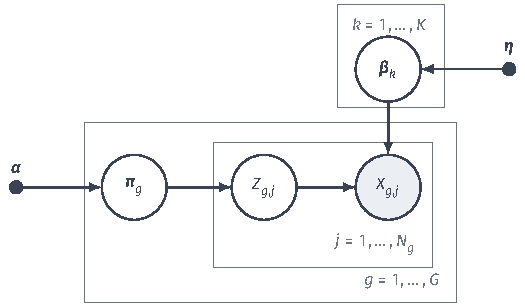
\includegraphics[width=88.935mm]{figures/06-probabilistic-graphical-models/04-models/tikz/pgm-static-directed-plates/figure.pdf}
  \caption{带全局主题先验的LDA重复结构。空心圆表示随机潜在量，填色圆表示观测词，实点表示给定超参数。文档板内每篇有一个$\bm\pi_g$，词板内每词有一组主题分配和观测；$K$个$\bm\beta_k$跨全部文档共享，词节点根据$Z_{g,j}$读取其中一个主题分布。}
  \label{fig:pgm-static-directed-plates}
\end{figure}

若按图~\ref{fig:pgm-static-directed-plates}为主题本身也设置先验，学习对象就改为
\[
 p(\bm\beta_{1:K},\bm\pi_{1:G},\bm z\mid\mathcal D,\bm\alpha,\bm\eta)
 \propto\prod_kp(\bm\beta_k\mid\bm\eta)
      \prod_g p(\bm\pi_g\mid\bm\alpha)
      \prod_{g,j}\pi_{g,z_{g,j}}\beta_{z_{g,j},x_{g,j}}.
\]
这个联合后验保留全局主题的不确定性，不能继续把$\bm\beta$的点参数更新当作同一推断目标。以下用折叠采样直接处理其主题分配。

在主题词分布也有Dirichlet先验的设定下，先积分掉$\bm\pi_g$和$\bm\beta_k$，再使用第~\ref{chap:pgm-sampling}章的Gibbs方法更新一个词的主题。排除当前位置后，文档主题计数记为$n_{g,k}^{-}$，全语料主题词计数为$c_{k,a}^{-}$，并记$c_{k,\cdot}^{-}=\sum_a c_{k,a}^{-}$、$\eta_0=\sum_a\eta_a$，单点条件为
\begin{equation}
  \label{eq:pgm-static-directed-lda-gibbs}
  p(Z_{g,j}=k\mid\text{其余分配},\mathcal{D})
     \propto (n_{g,k}^{-}+\alpha_k)
        \frac{c_{k,x_{g,j}}^{-}+\eta_{x_{g,j}}}
             {c_{k,\cdot}^{-}+\eta_0}.
\end{equation}
文档主题计数给出第一项，主题词计数给出第二项，二者是相应共轭后验的预测权重；文档分母与$k$无关，已经抵消。相乘并归一化，得到精确的单点条件分布。有限轮Gibbs样本构成的整体后验估计仍需考虑抽样误差和混合速度。

实际的一次扫描先从计数表移除当前位置原来的主题贡献，计算式~\eqref{eq:pgm-static-directed-lda-gibbs}的$K$个非负权重，再归一化抽取新主题，并把对应的文档主题计数和主题词计数加回。逐词重复扫描，丢弃初始过渡阶段并检查链的混合后，用保留状态作后验平均。对每个保留分配，可用$\bm\alpha+\bm n_g$与$\bm\eta+\bm c_k$恢复比例和主题的条件Dirichlet后验，再平均所需预测；不能把一个最终分配当成整个后验。

在对称主题先验下，同时置换主题编号和比例坐标，观测分布保持不变。非对称先验可约束部分编号，有限语料中的主题词分布仍可能有其他歧义；相近主题、短文档或过大的主题数会加剧不稳定性。词袋和比例先验各自限制了词序及组间变化，解释主题含义时，需要同时评价这些假设和分解的稳定性。

\subsection{随机成分库及其跨组共享}
\label{sec:pgm-static-directed-random-library}

前面的有限模型先固定可用成分数。现在把总体的成分库也看成未知量：先为一个总体建立随机混合测度，再让多个组共享它提供的原子、拥有不同使用比例。前一个问题由DPM处理，后一个问题再由HDP增加组层；DPM本身仍是单一总体模型。

\subsubsection{DPM：让数据中的占用成分参与推断}
\label{sec:pgm-static-directed-dpm-model}

前面的混合和主题模型都要求事先指定成分（主题）数$K$；$K$过小会欠拟合，过大则浪费容量并增加不稳定性。非参数贝叶斯方法不给成分库设固定上限，而在所有可能成分构成的空间上放置随机概率测度作为先验，使数据实际占用的成分数成为后验推断的一部分。有限混合和主题模型先给定候选成分数$K$。
\term{狄利克雷过程混合}（Dirichlet process mixture, DPM）为混合测度设置随机先验，让有限数据中的占用成分数参与推断。
在标准Borel成分参数空间上，记这个随机概率测度为$G\sim\operatorname{DP}(c,H)$。
其中$c>0$为浓度参数，基测度$cH$的总质量为$c$，$H$是基概率测度。若写作$\operatorname{DP}(\alpha,G_0)$，这里的参数对应为$\alpha=c$、$G_0=H$。
本节采用$c,H$，以区分主题比例先验的参数。
这里需要复用的有限分割规律是：对参数空间的任意有限可测分割$A_1,\ldots,A_m$，随机质量$(G(A_1),\ldots,G(A_m))$服从参数为$(cH(A_1),\ldots,cH(A_m))$的Dirichlet分布；零基质量的单元恒取零。这个规律使计数更新能够同时约束不同分辨率下的成分质量。


无穷多成分、权重总和为1的随机分布不便直接表示，折棒构造（stick-breaking construction）给出一种可数构造：取一根长度为1的棍，第$k$步按一个Beta随机比例从当前剩余棍段上截下一段作为成分$k$的权重，余下部分留给后续成分；反复截取而得的各段长度之和恰为1，由此得到混合建模可用的可数权重序列。
独立抽取$v_k\sim\operatorname{Beta}(1,c)$与$\bm\xi_k\sim H$，依次给剩余质量分配比例$v_k$，令
\[
  w_k=v_k\prod_{\ell<k}(1-v_\ell),\qquad
  G=\sum_{k=1}^{\infty}w_k\delta_{\bm{\xi}_k}.
\]
其中$\delta_{\bm\xi_k}$是原子处的点质量；折棒构造定理保证这个$G$具有上述有限分割规律。
权重和为$1$给出概率测度的归一化，Dirichlet过程分布还依赖这些分割规律。
Teh等的论述介绍了相应构造及其用于层次共享的方式\scite{pgm-static-directed-teh2006}
给定$G$，各记录独立抽取$\bm\zeta_j\mid G\sim G$，再按$\bm X_j\mid\bm\zeta_j\sim p(\cdot\mid\bm\zeta_j)$生成读数。
记录重复抽到一个原子，就使用同一成分参数；成分分布仍可连续。

DPM的学习目标是观测数据下的随机测度和记录分配后验，而非把候选数改大的固定维度最大似然。用$\Pi_{c,H}$表示DP先验律，其目标可写为
\begin{equation}
 p(dG,d\bm\zeta_{1:n}\mid\mathcal D)
 \propto \Pi_{c,H}(dG)\prod_{j=1}^n
       G(d\bm\zeta_j)\,p(\bm x_j\mid\bm\zeta_j).
 \label{eq:pgm-static-directed-dpm-posterior}
\end{equation}
给定读数时，占用成分的证据同时来自已有计数与该成分能否解释当前读数。下面先在成分参数已知的条件下计算DP更新，再把这个结果用于数据条件下的分配。

给定$n$个潜在成分参数，在任意有限分割上，用各单元的计数更新Dirichlet先验。
把这些相容的分割更新合在一起，得到随机测度的后验
\[
  G\mid\bm\zeta_{1:n}\sim\operatorname{DP}
    \left(c+n,\frac{cH+\sum_{j=1}^n\delta_{\bm\zeta_j}}{c+n}\right).
\]
下一条记录的成分参数预测分布由这个后验的均值给出。

取无原子的$H$并积分掉$G$，前$n$个潜在参数中占用成分$k$的计数为$n_k$，下一条复用它的概率为$n_k/(n+c)$，新抽成分的总概率为$c/(n+c)$。已有计数$(3,1)$、$c=1$时，三个选择分别为$0.6,0.2,0.2$。若该条读数也已给定，还需乘各已有成分和基准测度下的预测密度，再归一化。有限$n$至多占用$n$个成分，第$j$次增加成分的先验概率为$c/(c+j-1)$，所以占用数的先验期望是这些概率之和$\sum_{j=1}^n c/(c+j-1)$。可数先验放宽候选容量，实际推断处理当前占用或截断的候选成分，恢复真实有限类别数还需要其他条件。

在$H$与成分似然共轭的情形，可以积分掉$G$及各成分参数，直接更新记录的成分编号。把第$j$条记录移出后，令$n_k^{-j}$为剩余第$k$组的记录数，$\mathcal D_k^{-j}$为其数据。已有成分与新成分的未归一化权重分别是
\begin{equation}
 \begin{aligned}
 a_k&=n_k^{-j}\int p(\bm x_j\mid\bm\xi)
                              p(d\bm\xi\mid\mathcal D_k^{-j}),\\
 a_{\mathrm{new}}&=c\int p(\bm x_j\mid\bm\xi)H(d\bm\xi).
 \end{aligned}
 \label{eq:pgm-static-directed-dpm-allocation}
\end{equation}
先删除移出后变空的成分，再计算各预测密度、归一化这些权重并抽取新编号，最后写回计数与充分统计量；若选中新成分，则创建相应统计量。反复扫描得到占用数和预测分布的后验近似，成分参数需要时再从对应条件后验抽取。这说明$c/(n+c)$只是尚未读取新观测时的新建概率，不能直接用作给定读数后的分配概率。非共轭成分的预测积分可能不能解析完成，须再用数值积分、辅助变量或其他近似，并检查相应采样方法的有效性。

\subsubsection{HDP：使多个组共享同一套可数成分}
\label{sec:pgm-static-directed-hdp-model}

DPM解决了单组数据下成分数不定的问题，但在多组（多篇文档、多个工厂）场景下还有新问题：我们希望各组\emph{共享同一套}主题或成分，只是使用比例不同——不同文档讨论的应是同一批主题，而不是每篇文档各发明一套。若给每组单独抽一个Dirichlet过程，由于基测度连续，各组抽到的成分几乎必然互不相同，无法共享。解决办法是在组之上再加一层：先抽一个全局的随机成分库，再让每组的随机测度围绕这个全局库生成。多个组需要共享成分时，还要让它们使用相同原子。从同一个无原子$H$分别抽取独立Dirichlet过程，各组的原子几乎必然不同。\term{层次狄利克雷过程}（hierarchical Dirichlet process, HDP）取全局浓度参数$\gamma>0$，先抽离散的随机基准，再由它生成组测度：
\begin{equation}
  \label{eq:pgm-static-directed-hdp}
  G_0\sim\operatorname{DP}(\gamma,H),\qquad
  G_g\mid G_0\sim\operatorname{DP}(c,G_0).
\end{equation}
$G_0$几乎必然离散，所以各$G_g$共用同一可数原子集合，同时分别具有组级权重。在主题模型中，这些原子是词分布，每篇文档按自己的权重逐词选择共享主题。一个模型因此同时具有层次共享、混合成员及非固定成分数；这些属性描述不同的组织方式。Teh等进一步说明DP构造和HDP共享原子的机制\scite{pgm-static-directed-teh2006}

HDP的完整生成结构还包括$\bm\zeta_{g,j}\mid G_g\sim G_g$和$X_{g,j}\mid\bm\zeta_{g,j}\sim p(\cdot\mid\bm\zeta_{g,j})$。固定$c,\gamma,H$时，学习目标是全局测度、组测度及各项成分参数的联合后验：
\begin{equation}
 \begin{aligned}
 &p(dG_0,dG_{1:G},d\bm\zeta\mid\mathcal D)\\
 &\quad\propto\Pi_{\gamma,H}(dG_0)
     \prod_g\Pi_{c,G_0}(dG_g)
     \prod_{g,j}G_g(d\bm\zeta_{g,j})p(x_{g,j}\mid\bm\zeta_{g,j}).
 \end{aligned}
 \label{eq:pgm-static-directed-hdp-posterior}
\end{equation}
这里$G$在下标范围$1{:}G$中表示组数，$G_g$表示第$g$组的随机测度。条件于全局库，各组独立抽取权重；观测却会通过未知的全局库联系各组后验。与LDA相比，HDP既推断哪些主题被占用，也推断全局使用倾向怎样约束各文档比例，不能只把它理解为给固定主题数的LDA多加一个普通先验。

为把这个目标变成有限计算，下面在主题词模型中构造一个明确的截断近似。固定截断数$K$，取$v_k\sim\operatorname{Beta}(1,\gamma)$（$k<K$）并令$v_K=1$，把剩余折棒质量合并到最后一项，定义$w_k=v_k\prod_{\ell<k}(1-v_\ell)$。共享原子$\bm\xi_k$在这里是词概率向量，取$H=\operatorname{Dirichlet}(\bm\eta)$。每篇文档的组权重为$\bm\pi_g\mid\bm w\sim\operatorname{Dirichlet}(c\bm w)$，再按$Z_{g,j}\sim\operatorname{Categorical}(\bm\pi_g)$、$X_{g,j}\sim\operatorname{Categorical}(\bm\xi_{Z_{g,j}})$生成词。这个有限模型基于共享原子表示，但$K$有限时不同于原来的可数HDP，必须保留截断敏感性检查。

记全部未知量为$\Omega=(\bm v,\bm\xi,\bm\pi,\bm z)$，上述步骤对应明确的联合密度
\begin{equation}
 \begin{aligned}
 p_K(\mathcal D,\Omega)
 ={}&\prod_{k<K}\operatorname{Beta}(v_k;1,\gamma)
       \prod_{k=1}^K\operatorname{Dirichlet}(\bm\xi_k;\bm\eta)\\
 &\cdot\prod_g\operatorname{Dirichlet}(\bm\pi_g;c\bm w)
       \prod_{g,j}\pi_{g,z_{g,j}}\xi_{z_{g,j},x_{g,j}}.
 \end{aligned}
 \label{eq:pgm-static-directed-hdp-truncated-joint}
\end{equation}
采用平均场$q(\Omega)=\prod_{k<K}q(v_k)\prod_kq(\bm\xi_k)\prod_gq(\bm\pi_g)\prod_{g,j}q(Z_{g,j})$，其中折棒因子为Beta，词分布与组权重因子为Dirichlet，分配因子为类别分布。所有形状参数保持正值。具体的优化目标是
\begin{equation}
 \max_q\;\mathcal L_K(q)
   =\mathbb E_q[\log p_K(\mathcal D,\Omega)-\log q(\Omega)].
 \label{eq:pgm-static-directed-hdp-elbo}
\end{equation}
它下界化的是有限模型的$\log p_K(\mathcal D)$；提高该下界不能直接证明原可数模型的证据提高。这里把第~\ref{chap:pgm-variational}章的变分原理用于刚才写出的有限联合模型，不把以下计算称为原HDP的解析后验。

令$q(\bm\pi_g)=\operatorname{Dirichlet}(\bm a_g)$、$q(\bm\xi_k)=\operatorname{Dirichlet}(\bm\lambda_k)$、$q(Z_{g,j}=k)=r_{g,j,k}$。固定其余因子时，分别收集联合对数密度中含当前变量的项，可得
\begin{equation}
 \begin{aligned}
 r_{g,j,k}&\propto\exp\{\mathbb E_q\log\pi_{g,k}
                          +\mathbb E_q\log\xi_{k,x_{g,j}}\},\\
 a_{g,k}&=c\mathbb E_q[w_k]+\sum_jr_{g,j,k},\\
 \lambda_{k,a}&=\eta_a+\sum_{g,j}r_{g,j,k}\mathbb I\{x_{g,j}=a\}.
 \end{aligned}
 \label{eq:pgm-static-directed-hdp-local-vi}
\end{equation}
第一行对$k$归一化；两类对数期望与LDA一样由digamma差计算。组权重更新的先验伪计数是$c\mathbb E_q[w_k]$，而不是每组各自固定的一组$\alpha_k$；共享主题更新则汇集所有文档的词频。若$q(v_k)=\operatorname{Beta}(u_k,b_k)$，独立性给出$\mathbb E_q[w_k]=\mathbb E_q[v_k]\prod_{\ell<k}\mathbb E_q[1-v_\ell]$，其中$\mathbb E_q[v_k]=u_k/(u_k+b_k)$、$v_K=1$。

全局折棒的更新不能直接套用LDA计数公式。组先验的对数密度中包含以下依赖全局权重的项：
\[
 -\sum_k\log\Gamma(cw_k).
\]
它使全局权重与组权重之间不再共轭。固定其他变分因子后，可对Beta形状参数的对数$\bm\omega=(\log u_k,\log b_k)_{k<K}$数值优化$\mathcal L_K$。例如把其他因子的期望先汇总，记$A(\bm v)=\mathbb E_{q(\Omega\setminus\bm v)}\log p_K(\mathcal D,\Omega)$，在微分与积分可交换、梯度估计方差有限时，有
\[
 \nabla_{\bm\omega}\mathcal L_K
 =\mathbb E_{q_{\bm\omega}(\bm v)}
 [(A(\bm v)-\log q_{\bm\omega}(\bm v))
                     \nabla_{\bm\omega}\log q_{\bm\omega}(\bm v)].
\]
抽取折棒样本、计算括号内的全局与组先验项，再平均梯度并更新$\bm\omega$，就是前文评分函数估计在这个模型中的一项实现。概率接近边界时要检查数值精度和梯度方差；有限样本梯度更新不保证每一步ELBO上升。

完整训练循环因而包含：更新各词分配，汇总组权重与共享主题的参数，再优化全局折棒因子；随后回到各文档重算分配。初始化时使用正的形状参数，局部更新可多次迭代；停止时同时检查ELBO估计的变化及其蒙特卡洛波动，而不是仅比较相邻两次带噪数值。增大$K$后重新检查预测和尾部质量敏感性，分别报告截断近似、平均场近似与数值优化的限制。给已有文档预测新词，可用$\sum_k\mathbb E_q[\pi_{g,k}]\mathbb E_q[\xi_{k,a}]$；新文档则先从学得的全局权重及共享主题构造组先验，再结合其已观测词做局部推断。

DPM和HDP把有限数据占用的成分数、分配与随机权重纳入后验推断。以上演示固定浓度等超参数；若还要估计这些量，需要另加经验贝叶斯目标，或为它们设先验后扩大联合后验。截断变分用有限候选近似可数模型，需要检查截断误差；采样调整占用成分，需要检查链的混合。HDP还要共同处理组级成分和全局原子的关系，独立拟合各组有限混合无法完成这项共享推断。浓度参数影响分组倾向，需结合超参数估计和预测检验使用。输出时可报告预测、占用数及组间共享的不确定性，原子编号本身仍只承担命名。

\section{结构组合与查询选择}
\label{sec:pgm-static-directed-comparison}

本章模型沿两个维度变化：潜变量取值离散或连续，共享发生在记录内或跨组。比较时固定三条线索：面对一个查询，模型要对哪些随机量求和或积分、这些量在什么范围内共享、哪些非唯一性会限制对结果的解释；先固定查询与被积分的随机量，才能在同一口径下比较计算代价和适用场景。在表~\ref{tab:pgm-static-directed-comparison}中，给定所选全局参数或超参数，按各模型的设定汇总随机潜在量，得到观测似然$p(\bm x)$；用点估计固定的参数不再积分。NB和TAN的完整训练记录为$(y,\bm x)$，类别预测时则对$Y$归一化。独立性、共享和非唯一性另列，便于分析同一种查询在不同结构中需要完成哪些工作。

\begin{table*}[htbp]
  \centering
  \small
  \begin{tabularx}{\linewidth}{@{}
    >{\raggedright\arraybackslash}p{28mm}
    >{\raggedright\arraybackslash}p{30mm}
    >{\raggedright\arraybackslash}p{27mm}
    >{\raggedright\arraybackslash}p{30mm}
    >{\raggedright\arraybackslash}X@{}}
    \toprule
    模型与潜在量 & 独立性与共享 & 观测似然 & 局部后验 & 非唯一性与主要代价\\
    \midrule
    NB／TAN：训练时无潜变量 &
    类内独立／类内树；参数跨样本共享 &
    完整记录直接乘积 &
    类别后验枚举$K$项 &
    支持不足的条件表不确定；TAN还需选择树\\
    自回归：无随机潜变量 &
    顺序父集；条件网络可共享参数 &
    条件密度直接乘积 &
    前缀续写直接；任意补全未必易算 &
    网络参数可不唯一；优化、顺序选择与串行生成\\
    有限混合：离散分配 &
    样本在固定参数下独立；类内结构由成分决定 &
    $K$项有限和 &
    成分责任度精确 &
    标签交换、冗余成分；局部极值与退化\\
    FA／PPCA：连续因子 &
    给定因子后观测独立；共享载荷 &
    解析高斯密度 &
    解析高斯后验与缺失预测 &
    旋转及可能的额外分解歧义；维数与噪声假设\\
    LDA：连续比例与离散主题 &
    组级比例、全局主题；组内条件独立 &
    需积分比例，通常近似 &
    联合后验通常近似，局部条件可解析 &
    主题置换与重叠；局部推断和全局学习交替\\
    DPM／HDP：分配与随机测度 &
    可数候选成分；HDP跨组共享原子 &
    对未知随机量积分通常需近似 &
    采样或截断变分 &
    成分编号不唯一；占用数、超参数与近似误差\\
    \bottomrule
  \end{tabularx}
  \caption{静态有向模型在给定参数或超参数下的计算。表中的精确结果指相应有限求和、解析积分或局部条件；学习目标、参数不确定性及潜在解释另按各模型分析。}
  \label{tab:pgm-static-directed-comparison}
\end{table*}

直接模型以局部条件拟合观测联合分布。NB用类内独立减少待估参数，TAN增加树边及结构搜索，神经自回归则用非线性条件与参数共享扩大可表达的关系。完整记录可直接计算局部乘积，祖先生成和缺失查询还需按各自依赖进行。潜变量路线也可能保留精确计算：有限混合显式汇总$K$项，线性高斯模型解析积分，同时给出似然和局部后验。

共享随机量会联系不同位置的推断。pLSA固定文档比例时，逐词做有限求和；LDA积分共同的文档比例后，主题分配需要一起解释这些词。全局主题再带先验时，不同文档也相互联系，HDP还需要推断共享的占用成分。这些联系决定了联合后验的规模，除各变量的状态数外，还需考察它们共同读取哪些数据。

模型之间的联系还要落到结构和学习对象的变化上。NB与TAN都保留类别生成属性的结构，TAN只放宽类内父集；把NB的训练类别隐藏，并保留原来的条件乘积，就得到乘积分布的有限混合。这里改变的是类别的观测状态，所以已知计数变成需要E步计算的后验期望计数。FA到PPCA则没有改变观测状态，而是把逐维噪声约束为同一个方差；两者都约束协方差的低秩加噪声分解。下一章的高斯马尔可夫随机场将转而约束精度矩阵的零元素，二者对同一高斯分布族施加不同结构限制。自回归网络的三种实现都保留顺序条件乘积，掩码和卷积改变条件函数的计算及参数共享。

有限混合与混合成员的区别在分配单位：前者一条记录选择一个成分，后者在一组内部逐项选择。pLSA到LDA进一步把文档比例由固定参数变为随机量，因此新文档有了比例先验，也增加了比例积分。DPM对单一总体引入随机成分库；HDP在这个库之上增加组权重，让不同组共享原子而保持不同使用比例。这些变化分别作用于容量、共享和分配单位，不能排成一条每个模型都替代前者的升级链。

表~\ref{tab:pgm-static-directed-learning-map}补充各分支的目标和更新对象，与表~\ref{tab:pgm-static-directed-comparison}的查询成本合读，可以区分“模型怎样表示”“参数怎样学到”和“训练后怎样使用”。
\begin{table*}[htbp]
 \centering\small
 \begin{tabularx}{\linewidth}{@{}p{25mm}XXX@{}}
 \toprule
 模型 & 结构改变与动机 & 学习目标 & 具体更新对象\\
 \midrule
 NB／TAN & 类内独立或属性树减少条件表规模 & 带标签联合似然；TAN另选树 & 类别与父配置计数；条件互信息最大生成树\\
 NADE／MADE／PixelCNN & 前缀复用、掩码与空间共享控制条件函数 & 完整记录自回归负对数似然 & 由各位置梯度共同更新网络权重\\
 有限混合／GMM & 用未知离散成分解释多种模式 & 成分求和后的观测似然 & 责任度、加权均值与协方差交替更新\\
 FA／PPCA & 连续共同强度与独有噪声分解相关 & 低秩加噪声高斯似然 & 后验一、二阶矩，载荷与受约束噪声\\
 层次正态 & 组参数共享总体且保留差异 & 组边缘似然或联合后验 & 组后验矩与超参数；或联合采样、变分\\
 pLSA／LDA & 逐词分配；固定或随机文档比例 & pLSA似然、LDA的ELBO或联合后验 & 文档比例、主题词频；LDA另推断比例或折叠分配\\
 DPM／HDP & 随机成分库；HDP跨组共享原子 & 随机测度联合后验；有限近似的ELBO & 分配、成分、组权重及全局权重\\
 \bottomrule
 \end{tabularx}
 \caption{建模选择与学习计算的对应。表中并列的目标属于不同设定，使用某一模型时须先选定点参数估计或贝叶斯后验目标，再采用相应更新。}
 \label{tab:pgm-static-directed-learning-map}
\end{table*}

也可以组合上述属性。混合因子分析为每个离散成分配置连续因子，成分内积分后仍是低秩加对角协方差的高斯，所以成分责任度和因子后验可解析计算。自回归条件可采用有限混合，组级载荷可设置层次先验。因此离散或连续、线性高斯或非线性、组间共享或独立、逐项生成或联合生成，分别描述模型的一项选择。

观测分布估计准确时，潜在解释仍可能受对称性约束：网络权重可有多种表示，成分可交换编号，因子可旋转方向。选择模型时，可先用留出数据评价预测，再按目的检查所需输出；解释结构需要报告对称性及稳定性，补全任务则需要评价条件预测和误差范围。似然计算、预测表现和潜在语义各有相应的核验对象。

\section{本章小结}
\label{sec:pgm-static-directed-summary}

本章把表示、推断和学习组装到具体的静态有向模型上，并沿三条主线展开：观测之间的直接依赖、记录内部由潜变量给出的共同解释、以及跨记录跨组的共享。静态有向分解把局部条件组合成联合分布。全部变量可观测时直接读取乘积，引入潜在状态后则先汇总它们，得到观测分布。两个传感器的同一联合表可用自回归条件或隐藏类别的混合表示，前者给出读数预测次序，后者加入需要另行验证的工作状态解释。

有限混合用责任度与成分参数交替学习，固定参数的局部后验仍可精确求得。线性高斯积分把观测协方差、降维和缺失预测联系起来；共享随机量与混合成员联系多个记录或组的推断，联合计算可能需要近似。取值类型与共享方式可以组合使用，标签置换、因子旋转和其他分解歧义则限制了潜在坐标的唯一解释。

判断新模型时，可以从联合归一化、查询待消变量、共享范围和估计的边界条件逐项展开。若建模依据首先是变量状态之间的相容性，可以改用局部相容函数与统一归一化，而不必先指定谁生成谁。第~\ref{chap:pgm-energy-models}章据此比较联合归一化与输出条件归一化；这是一种表示选择，不意味着有向分解不能表达对称的观测分布。第~\ref{chap:pgm-generative}章再以自回归和高斯潜变量为参照，讨论神经网络如何参数化更灵活的密度，以及相应概率计算的代价。

\paragraph{扩展阅读}
Bishop的PRML用混合、潜变量及变分学习展开静态模型，Koller与Friedman从局部条件结构讨论共同的推断与学习方法。可沿同一图的作用域比较不同局部分布，检查哪些求和或积分仍有解析形式，哪些学习目标需要近似后验\scite{bishop2006,pgm-koller2009}

\chapter{静态无向模型}
\label{chap:pgm-energy-models}

相邻检测位置可能同时过热，也可能受到同一测量干扰，整排状态因而需要联合考虑。给定各位置的相对偏好以及相邻状态的相容权重，怎样计算整排配置的概率？若温度读数已知、只需预测异常标签，是否还要同时建立这些读数的生成分布？

两项任务都可以组合局部势，区别在于哪些变量参与归一化。联合无向模型比较全部建模变量的配置，条件无向模型则固定输入、只比较输出。局部无向分解规定了变量在给定分隔节点后的独立关系（参见第~\ref{chap:pgm-undirected}章）；本章据此构造具体模型，说明结构怎样影响推断，以及潜变量、高阶势和神经参数化各带来哪些表达能力与计算要求。联合与条件是本章的主要划分；变量是否可见、势是否成对以及参数化方式可以组合。

\section{无向模型的共同形式}
\label{sec:pgm-energy-models-common}

先为整排状态规定无向图$\mathcal{G}=(V,E)$，令$d=|V|$、$\bm{X}=(X_1,\ldots,X_d)^\top$。局部配置越符合建模偏好，其\term{势函数}（potential function）值越大；这个值表示相对相容程度，无须自身求和为$1$。记因子作用域集合为$\mathcal{C}$，每个$C\in\mathcal{C}$取图中的一个团，允许使用非极大团。将严格正势$\psi_{\bm{\theta},C}$写成局部能量$E_{\bm{\theta},C}=-\log\psi_{\bm{\theta},C}$，乘积权重便转为能量之和：
\begin{equation}
  \begin{aligned}
    E_{\bm{\theta}}(\bm{x})
      &=\sum_{C\in\mathcal{C}}E_{\bm{\theta},C}(\bm{x}_C),\\
    p_{\bm{\theta}}(\bm{x})
      &=\frac{\prod_{C\in\mathcal{C}}
               \psi_{\bm{\theta},C}(\bm{x}_C)}
              {Z_{\bm{\theta}}}
        =\frac{\exp[-E_{\bm{\theta}}(\bm{x})]}{Z_{\bm{\theta}}},\\
    Z_{\bm{\theta}}
      &=\int \exp[-E_{\bm{\theta}}(\bm{u})]\,\mathrm{d}\mu(\bm{u}).
  \end{aligned}
  \label{eq:pgm-energy-models-joint}
\end{equation}
参数向量$\bm{\theta}$包含各局部势的参数。离散状态采用计数测度$\mu$，连续状态采用指定基准测度，通常是Lebesgue测度。\term{能量函数}（energy function）的值越低，配置的未归一化权重越大；\term{配分函数}（partition function）$Z_{\bm{\theta}}$累加或积分全部权重，使其成为概率，故须满足$0<Z_{\bm{\theta}}<\infty$。这里使用无量纲的对数权重，物理模型的逆温度已计入参数。

也可以用负能量$f_{\bm{\theta}}=-E_{\bm{\theta}}$给配置评分，对数概率还需扣除$\log Z_{\bm{\theta}}$。增加与$\bm{x}$无关的能量常数，会等比例缩放全部权重及配分函数，概率保持原值。按正比例缩放能量时，配置间的能量差也同比例变化；比例不为$1$且两个配置的能量不同时，它们的概率比会改变。若只比较固定模型中的两种配置，配分函数可从比值中消去：
\[
  \frac{p_{\bm{\theta}}(\bm{x})}{p_{\bm{\theta}}(\bm{x}')}
  =\exp\{E_{\bm{\theta}}(\bm{x}')-E_{\bm{\theta}}(\bm{x})\}.
\]
因此，能量差能够排序配置，绝对概率仍依赖全部权重的总量。改变局部势的状态偏好时，配分函数也可能改变；即使某个配置的未归一化权重不变，其概率仍可能随归一化而改变。

若测量输入$\bm{x}$已经固定、待预测量为$\bm{Y}$，需要比较的候选只有输出配置。相同能量构造此时只在输出空间归一化：
\begin{equation}
  \begin{aligned}
    p_{\bm{\theta}}(\bm{y}\mid\bm{x})
      &=\frac{\exp[-E_{\bm{\theta}}(\bm{y},\bm{x})]}
              {Z_{\bm{\theta}}(\bm{x})},\\
    Z_{\bm{\theta}}(\bm{x})
      &=\int\exp[-E_{\bm{\theta}}(\bm{v},\bm{x})]
                  \,\mathrm{d}\mu_Y(\bm{v}).
  \end{aligned}
  \label{eq:pgm-energy-models-conditional}
\end{equation}
每个使用的输入都须给出$0<Z_{\bm{\theta}}(\bm{x})<\infty$。该式只定义输出的条件概率，没有为输入规定$p(\bm{x})$，也不限制输入之间的依赖。附加只依赖输入的能量$c(\bm{x})$时，它在分子、分母中消去。图~\ref{fig:pgm-energy-models-normalization}据此区分输入的两种职责：它可以改变各势的数值，却不参与输出的求和。

\begin{figure}[htbp]
  \centering
  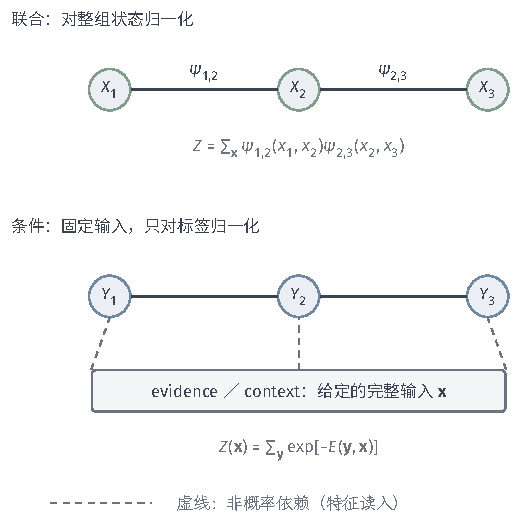
\includegraphics[width=86.907mm]{figures/06-probabilistic-graphical-models/04-models/tikz/pgm-energy-models-normalization/figure.pdf}
  \caption{三节点相互作用的两种归一化。上方联合模型对全部状态求和；下方把$\bm{x}$列为给定证据或条件输入，只对标签$\bm{y}$求和。灰底框中的输入通过虚线影响标签势，虚线表示特征依赖，不表示有向生成关系。}
  \label{fig:pgm-energy-models-normalization}
\end{figure}

有限离散状态配合有限能量，必然产生正且有限的配分函数。连续能量则需检查尾部：即使$E(x)=-x^2$处处有定义，$\int_{\mathbb{R}}e^{x^2}\,\mathrm{d}x$仍发散。允许势为零时，可以用$+\infty$能量排除配置，但归一化还须有正总权重；离散支持至少保留一个正权配置，连续支持则需有正测度。因子分解仍能给出相应Markov性质，而从Markov性质反推分解的正性定理不能直接用于零势（参见第~\ref{chap:pgm-undirected}章）。

\section{联合能量模型}
\label{sec:pgm-energy-models-joint-models}

为整组测量状态建立联合分布，可以用于补全状态、计算多变量事件概率或生成配置。以下先取成对作用，再分别引入隐藏状态、改变能量函数或扩大因子作用域。它们共同使用式~\eqref{eq:pgm-energy-models-joint}，推断时能利用的分解与代数形式却各不相同。

\subsection{观测变量成对模型}
\label{sec:pgm-energy-models-pairwise}

对只有两种状态的检测位置，取$x_i\in\{-1,+1\}$。\term{Ising模型}（Ising model）分别用单点参数表示状态偏好，用边参数表示相邻状态同号或异号的偏好：
\begin{equation}
  E_{\bm{\theta}}(\bm{x})
    =-\sum_{i\in V}b_ix_i
     -\sum_{\{i,j\}\in E}J_{i,j}x_ix_j.
  \label{eq:pgm-energy-models-ising}
\end{equation}
\term{外场}（external field）$b_i$取正值时偏好$+1$。\term{耦合参数}（coupling parameter）$J_{i,j}$取正值时奖励同号，取负值时奖励异号；每条无向边只计一次，约定$J_{i,j}=J_{j,i}$。这些参数描述统计相容性，不能仅凭它们推断干预一个位置对另一位置的效应。

要计算一个位置的条件概率，固定其余状态，仅保留含$x_i$的得分$x_i(b_i+\sum_{j\in N(i)}J_{i,j}x_j)$，其中$N(i)$为邻居集合。$+1$与$-1$的权重比为$\exp[2(b_i+\sum_jJ_{i,j}x_j)]$，归一化两项后得到
\begin{equation}
  \begin{aligned}
    p_{\bm{\theta}}(X_i=+1\mid\bm{x}_{V\setminus\{i\}})
      &=\sigma\!\left(2b_i+
           2\sum_{j\in N(i)}J_{i,j}x_j\right),\\
    \sigma(u)&=\frac{1}{1+e^{-u}}.
  \end{aligned}
  \label{eq:pgm-energy-models-ising-conditional}
\end{equation}
这个满条件分布只读取邻居状态。移去这些条件以后，无直接边的两个节点仍可能经其他节点相关。

用三个相邻位置构造数值例子：图取$1-2-3$，不设单点偏好，同号边势为$3$、异号边势为$1$。这些是人为指定的权重，尚未归一化为概率。为计算联合权重，先统计相邻同号对：
\[
  N_{=}(\bm{x})
   =\mathbf{1}\{x_1=x_2\}+\mathbf{1}\{x_2=x_3\}.
\]
令$E_0(\bm{x})=-(\log3)N_{=}(\bm{x})$，配置权重就是$3^{N_{=}(\bm{x})}$。首节点可取两个值，每个后继节点的两项权重和为$3+1=4$，故$Z_0=2\times4\times4=32$。由$\mathbf{1}\{x_i=x_j\}=(1+x_ix_j)/2$，这也对应$J_{1,2}=J_{2,3}=(\log3)/2$的Ising分布。两种能量约定相差常数：$E_0$比式~\eqref{eq:pgm-energy-models-ising}的零外场能量少$\log3$，后者的配分函数为$32/3$。概率相同，配分函数数值则随能量常数而变。

在该对称链中，给定一个位置，后继位置同号和异号的条件概率分别为$3/4$、$1/4$。两端同号对应两次保持或两次翻转，因而
\[
  p(X_3=X_1\mid X_1)
    =(3/4)^2+(1/4)^2=\frac58.
\]
各节点的边缘都为均匀二值分布，所以$\mathbb{E}[X_1X_3]=2(5/8)-1=1/4$。两端虽无边仍相关，给定$X_2$才独立。将同样参数用于更长的零外场链，每跨一条边，条件均值乘以$1/2$，相隔$r$条边的相关为$(1/2)^r$。这说明相互作用能够沿路径传递，其强度还由参数决定。

类别数增加到$K>2$后，标签编号的乘积无法直接表示相容性。\term{Potts模型}（Potts model）改为比较类别是否相等，对$x_i\in\{1,\ldots,K\}$定义
\begin{equation}
  E_{\bm{\theta}}(\bm{x})
   =-\sum_i b_i(x_i)
    -\sum_{\{i,j\}\in E}J_{i,j}\mathbf{1}\{x_i=x_j\}.
  \label{eq:pgm-energy-models-potts}
\end{equation}
$b_i(k)$规定位置$i$对类别$k$的偏好。计算节点条件分布时，固定邻居，为每个类别$k$形成权重
\[
  w_i(k)=\exp\left\{
    b_i(k)+\sum_{j\in N(i)}J_{i,j}\mathbf{1}\{k=x_j\}
  \right\},
\]
将权重除以$\sum_{\ell=1}^K w_i(\ell)$即得满条件概率。每条边只用一个参数区分类别相同与不同，限制了它能表达的相容关系；特定异类组合有不同偏好时，需改用$K\times K$边势表。二类Potts可以重新编码为Ising，其中耦合系数需按前述$1/2$因子换算。

完整观测提供单点状态以及边上的乘积或同类指示。固定图、存在有限内点最大似然解时，模型期望与对应经验统计量匹配；例如$J_{i,j}$的似然梯度使用经验$x_ix_j$减去$\mathbb{E}[X_iX_j]$（通用推导及替代准则参见第~\ref{chap:pgm-parameter-learning}章）。Ising的解析满条件还能直接用于Gibbs更新和伪似然拟合。强耦合时，单点变化难以转到另一种整体配置，采样仍可能很慢。

一般稠密边势在树上求配分函数与边缘需$O(dK^2)$运算，特殊边势可能进一步简化。一般图则受消元后的诱导宽度限制，原始因子成对不保证全局计算只有二次成本。二值吸引型模型可以通过图割求最优配置，但这一最大化未计算配分函数（参见第~\ref{chap:pgm-variational}章）。参数也会限制模型适用性：过强的同号偏好可能掩盖局部异常；三角形的每条边都偏好异号时，任一二值配置至少违背一项偏好。

温度等连续状态可以用二次能量描述。\term{高斯Markov随机场}（Gaussian Markov random field, GMRF）通过精度矩阵表示条件依赖；对$\bm{x}\in\mathbb{R}^d$取
\begin{equation}
  \begin{aligned}
    E_{\bm{\theta}}(\bm{x})
      &=\frac12(\bm{x}-\bm{\mu})^\top
                    \bm{Q}(\bm{x}-\bm{\mu}),\\
    Z_{\bm{\theta}}
      &=(2\pi)^{d/2}|\bm{Q}|^{-1/2},
      \qquad \bm{Q}=\bm{Q}^\top\succ0.
  \end{aligned}
  \label{eq:pgm-energy-models-gaussian}
\end{equation}
均值为$\bm{\mu}$，协方差的逆$\bm{Q}$称为\term{精度矩阵}（precision matrix）。正定性使二次能量在所有方向增长，并使高斯积分有限。为补全一个未知位置，给定其余位置后的分布为
\[
  \begin{aligned}
    \widetilde{\mu}_i(\bm{x})
      &=\mu_i-\frac{1}{Q_{i,i}}
           \sum_{j\ne i}Q_{i,j}(x_j-\mu_j),\\
    X_i\mid\bm{x}_{V\setminus\{i\}}
      &\sim\mathcal{N}\!\left(
          \widetilde{\mu}_i(\bm{x}),Q_{i,i}^{-1}\right).
  \end{aligned}
\]
$\widetilde{\mu}_i$是给定其余节点后的条件均值。在非退化高斯模型中，$Q_{i,j}=0$恰好对应$X_i\perp X_j\mid\bm{X}_{V\setminus\{i,j\}}$；协方差为零判别的则是边缘独立，两者不可互换（证明参见第~\ref{chap:pgm-undirected}章）。

仍取三个检测位置，用中心化并缩放后的温度构造零均值模型，令
\[
  \bm{Q}=
  \begin{pmatrix}
    2&-1&0\\ -1&2&-1\\ 0&-1&2
  \end{pmatrix},
  \qquad
  \bm{Q}^{-1}=\frac14
  \begin{pmatrix}
    3&2&1\\ 2&4&2\\ 1&2&3
  \end{pmatrix}.
\]
$\bm{Q}$的顺序主子式为$2,3,4$，所以它正定。两端精度为零，协方差却为$1/4$，展示了中点传递的边缘相关。给定$x_1=2,x_3=0$，中点分布为$\mathcal{N}(1,1/2)$；以条件均值补全得到$1$，条件方差则量化补全后仍有的不确定性。

高斯推断主要使用线性求解和矩阵分解。稠密Cholesky分解耗时$O(d^3)$，随后可计算条件均值、所需协方差及对数行列式；链状精度具有固定带宽时，分解可随$d$线性增长。一般稀疏矩阵可能产生消元填充，原始零元素数量因此不足以判定时间成本。学习时，若均值已知为零，取样本二阶矩$\bm{S}=n^{-1}\sum_{r=1}^n\bm{x}_r\bm{x}_r^\top$，要最大化的精度相关对数似然为
\[
  \frac n2\{\log|\bm{Q}|-\operatorname{tr}(\bm{S}\bm{Q})\},
  \qquad \bm{Q}\succ0,
\]
缺边对应$Q_{i,j}=0$，这些约束与正定性共同限定候选精度。无图约束且$\bm{S}\succ0$时，最优解是$\bm{S}^{-1}$；有零约束时通常需要约束优化。仅半正定的精度不能在整个$\mathbb{R}^d$上归一化为式~\eqref{eq:pgm-energy-models-gaussian}，单个高斯也无法表达多峰。解析计算的便利伴随这些表示条件，延长优化迭代不能消除它们\scite{pgm-undirected-rue2005}

\subsection{潜变量能量模型}
\label{sec:pgm-energy-models-latent}

共同异常也可能来自未测状态。可以让一个潜变量连接多个可见位置，先建立联合分布，再将它边缘化。\term{玻尔兹曼机}（Boltzmann machine, BM）采用二值变量的成对能量实现这一构造。以下改用$0/1$编码：可见量为$\bm{x}\in\{0,1\}^{d_{\mathrm{v}}}$，隐藏量为$\bm{z}\in\{0,1\}^m$，共有$d_{\mathrm{v}}+m$个节点：
\begin{equation}
  \begin{aligned}
    E_{\bm{\theta}}(\bm{x},\bm{z})
      &=-\bm{b}^\top\bm{x}-\bm{c}^\top\bm{z}
        -\bm{x}^\top\bm{W}\bm{z}\\
      &\quad-\frac12\bm{x}^\top\bm{U}\bm{x}
             -\frac12\bm{z}^\top\bm{R}\bm{z},\\
    p_{\bm{\theta}}(\bm{x},\bm{z})
      &=\frac{e^{-E_{\bm{\theta}}(\bm{x},\bm{z})}}
               {Z_{\bm{\theta}}},\\
    p_{\bm{\theta}}(\bm{x})
      &=\sum_{\bm{z}}p_{\bm{\theta}}(\bm{x},\bm{z}).
  \end{aligned}
  \label{eq:pgm-energy-models-bm}
\end{equation}
$\bm{W}\in\mathbb{R}^{d_{\mathrm{v}}\times m}$连接可见与隐藏节点，$\bm{U}$、$\bm{R}$分别连接各组内部，二者对称且对角为零。组内项乘$1/2$以避免重复计边。一般BM即使固定全部可见量，隐藏节点仍有相互作用；训练所需的数据后验期望和无条件模型期望都可能依赖近似推断。

若要直接计算隐藏后验，可以删除两组各自内部的边，令$\bm{U}=\bm{0}$、$\bm{R}=\bm{0}$。这就是\term{受限玻尔兹曼机}（restricted Boltzmann machine, RBM）的二部限制：固定一组以后，另一组的节点没有剩余相互作用。记$u_j(\bm{x})=c_j+\sum_iW_{i,j}x_i$，隐藏条件分布分解为
\[
  p_{\bm{\theta}}(\bm{z}\mid\bm{x})
   =\prod_{j=1}^m\frac{\exp[z_ju_j(\bm{x})]}
                         {1+\exp[u_j(\bm{x})]}.
\]
每个分母都由$z_j=0,1$的两个权重相加得到，条件分布因而按节点独立。交换两组可得相应的可见条件分布：
\begin{equation}
  \begin{aligned}
    p_{\bm{\theta}}(Z_j=1\mid\bm{x})
      &=\sigma\!\left(c_j+\sum_iW_{i,j}x_i\right),\\
    p_{\bm{\theta}}(X_i=1\mid\bm{z})
      &=\sigma\!\left(b_i+\sum_jW_{i,j}z_j\right).
  \end{aligned}
  \label{eq:pgm-energy-models-rbm-conditionals}
\end{equation}
这些sigmoid表达没有Ising满条件的系数$2$，因为变量已经由$\{-1,+1\}$改为$0/1$编码。

二部限制还简化了隐藏变量的求和。对固定可见配置，\term{自由能}（free energy）取全部隐藏配置权重和的负对数，得到可见分布的有效能量；它汇总隐藏状态，而非只取最优隐藏状态：
\begin{equation}
  \begin{aligned}
    F_{\bm{\theta}}(\bm{x})
      &:=-\log\sum_{\bm{z}}
                 e^{-E_{\bm{\theta}}(\bm{x},\bm{z})}\\
      &=-\bm{b}^\top\bm{x}
        -\sum_{j=1}^m\log(1+e^{u_j(\bm{x})}),\\
    p_{\bm{\theta}}(\bm{x})
      &=\frac{e^{-F_{\bm{\theta}}(\bm{x})}}{Z_{\bm{\theta}}}.
  \end{aligned}
  \label{eq:pgm-energy-models-free-energy}
\end{equation}
隐藏求和可拆成$\sum_{\bm{z}}\prod_j e^{z_ju_j}=\prod_j(1+e^{u_j})$，这给出了自由能公式。隐藏节点连接多个可见节点时，消元后的一项$\log(1+e^{u_j})$通常同时依赖它们。因此，联合模型中的成对作用可以成为可见边缘中的高阶势（图~\ref{fig:pgm-energy-models-rbm}）。

\begin{figure}[htbp]
  \centering
  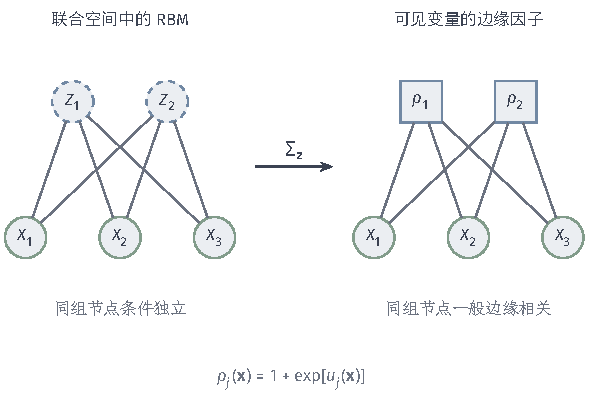
\includegraphics[width=99.653mm]{figures/06-probabilistic-graphical-models/04-models/tikz/pgm-energy-models-rbm/figure.pdf}
  \caption{RBM的条件分解与隐藏消元。左侧仅有跨组边，固定一组时另一组条件独立；右侧把两个隐藏节点消去，两个因子$1+\exp[u_j(\bm{x})]$各涉及三个可见变量。一元可见偏置势在两侧均省略。可见边缘仍可能相关。}
  \label{fig:pgm-energy-models-rbm}
\end{figure}

取两个可见节点和一个隐藏节点，偏置均为零，$W_{1,1}=W_{2,1}=\log2$。可见权重为$e^{-F(\bm{x})}=1+2^{x_1+x_2}$，配置$(0,0),(0,1),(1,0),(1,1)$的权重依次为$2,3,3,5$，总和为$13$。给定$(x_1,x_2)=(1,1)$，隐藏状态为$1$的概率是$4/5$。给定$z=0$时，两可见节点独立、取$1$概率各为$1/2$；给定$z=1$时，该概率各为$2/3$。消去隐藏状态后，$p(X_1=X_2=1)=5/13$与$p(X_1=1)p(X_2=1)=(8/13)^2$相差$1/169$，独立性没有保留。

单个可见配置的自由能求值为$O(d_{\mathrm{v}}m)$，其权重总和$Z_{\bm{\theta}}=\sum_{\bm{x}}e^{-F_{\bm{\theta}}(\bm{x})}$通常仍需指数计算。枚举较小的一组、解析消去另一组虽可减少运算，仍含$2^{\min(d_{\mathrm{v}},m)}$规模。RBM使完整可见配置下的隐藏后验可算，没有普遍消除联合归一化成本。部分可见量未测时，$p(\bm{z}\mid\bm{x}_{\mathrm{obs}})$也未必保有上述独立Bernoulli分解。

这两个块条件可以构成\term{交替Gibbs采样}（alternating Gibbs sampling）：固定一组，独立随机抽取另一组，再交换两组。算法~\ref{alg:pgm-energy-models-rbm-gibbs}传递的是抽到的二值状态；若直接传递概率，所得确定性迭代已不再使用这个Gibbs核。

\begin{algorithm}[RBM的一段交替Gibbs链]
  \label{alg:pgm-energy-models-rbm-gibbs}
  \begin{algorithmic}[1]
    \Require 固定的有限参数$\bm{\theta}$，初始状态$\bm{x}^{(0)}$，步数$k\geq1$
    \Ensure 链状态$\bm{x}^{(1)},\ldots,\bm{x}^{(k)}$
    \For{$t=0,\ldots,k-1$}
      \State 按式~\eqref{eq:pgm-energy-models-rbm-conditionals}独立抽取各$Z_j^{(t+1)}$
      \State 固定$\bm{z}^{(t+1)}$，独立抽取各$X_i^{(t+1)}$
    \EndFor
  \end{algorithmic}
\end{algorithm}

固定有限参数下，每个块条件概率都在$0$与$1$之间，可见状态链因而能到达任意配置，并有自转移。交替Gibbs核保持$p_{\bm{\theta}}(\bm{x})$不变，有限不可约、非周期链的分布遂长期收敛到它；这并未给出小$k$充分混合的保证（参见第~\ref{chap:pgm-sampling}章）。完整一次更新为$O(d_{\mathrm{v}}m)$，强权重形成的近确定条件可能使链长期停留在同一模式。

训练一个权重时，需要提高数据配置的概率，同时扣除模型自身的联合统计。对单条数据$\bm{x}$，潜变量似然梯度在RBM中写为（通用推导参见第~\ref{chap:pgm-parameter-learning}章）
\begin{equation}
  \frac{\partial\log p_{\bm{\theta}}(\bm{x})}
       {\partial W_{i,j}}
    =x_i\,p_{\bm{\theta}}(Z_j=1\mid\bm{x})
      -\mathbb{E}_{p_{\bm{\theta}}}[X_iZ_j].
  \label{eq:pgm-energy-models-rbm-gradient}
\end{equation}
数据项由隐藏条件概率精确取得，模型项则通常需要采样。多条记录对数据项求平均，偏置的梯度对应一阶统计量。RBM简化的是给定数据的后验计算，模型期望仍然存在。重构误差与似然也有不同含义：慢混合的短链容易留在起始数据附近，却可能没有正确分配不同模式的概率质量\scite{pgm-energy-models-hinton2010}

图~\ref{fig:rbm-alternating-sampling-and-gradient}按这一顺序区分概率、抽样状态与训练统计：先固定参数运行交替链、估计模型统计，再用数据统计减模型统计更新参数。

\begin{figure*}[htbp]
  \centering
  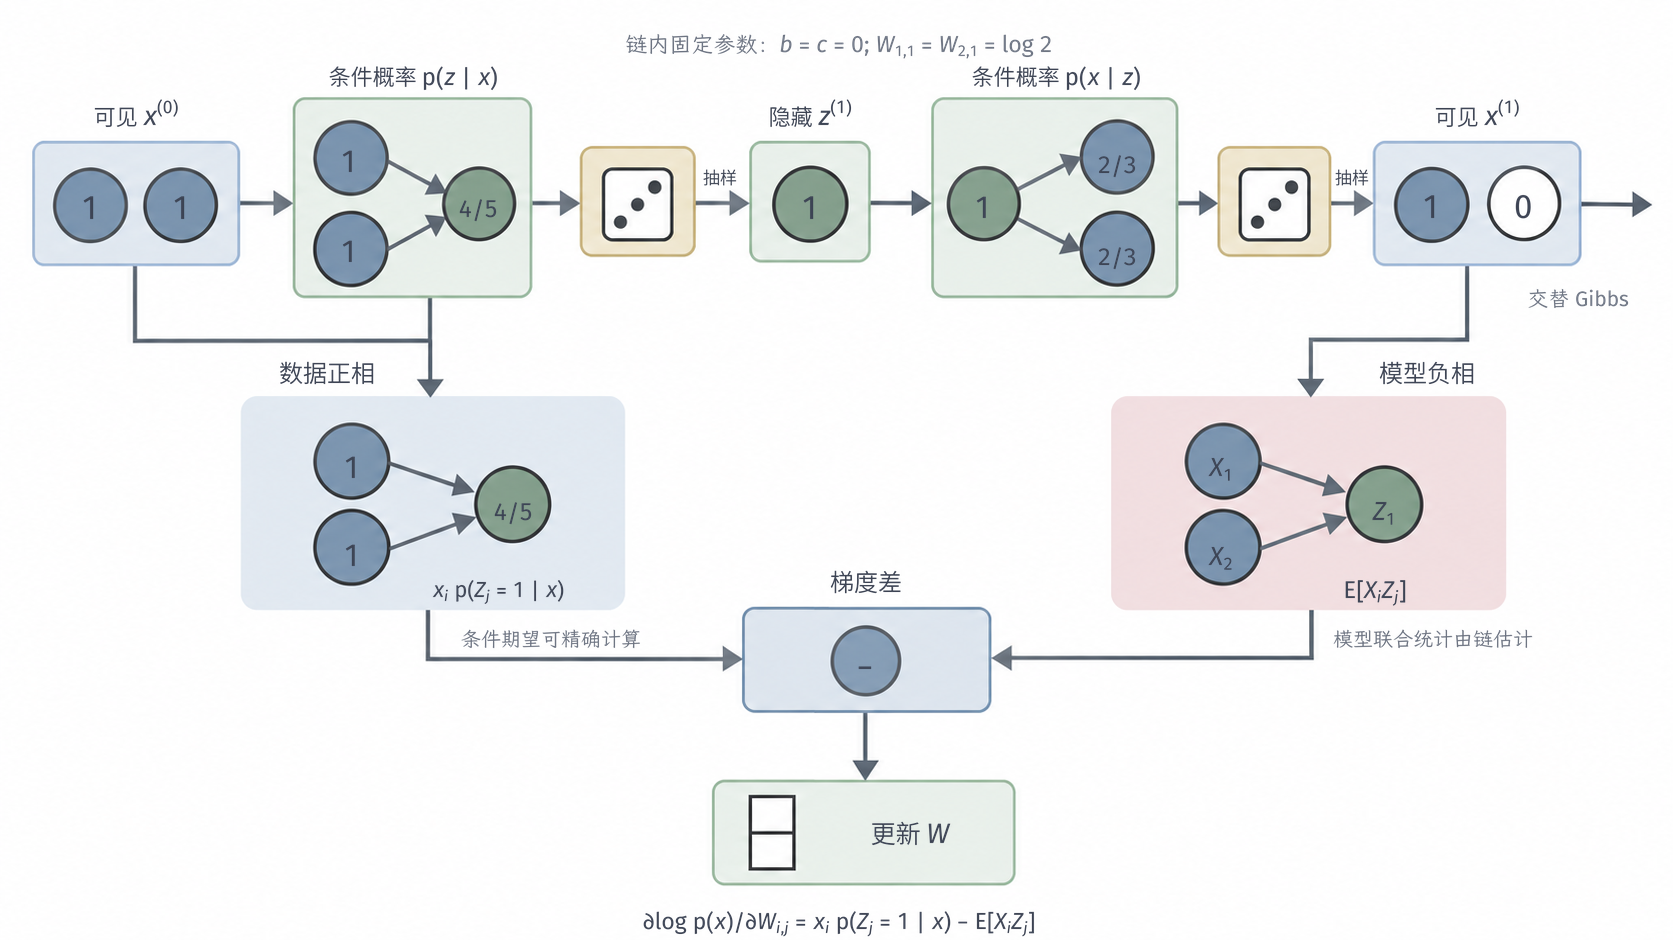
\includegraphics[width=141.647mm]{figures/06-probabilistic-graphical-models/04-models/generated/rbm-alternating-sampling-and-gradient/figure.png}
  \caption{二值RBM中的抽样状态和训练统计。取$b=c=0$、$W_{1,1}=W_{2,1}=\log2$，可见状态$(1,1)$对应隐藏条件概率$4/5$；若抽到$z=1$，可见单元的条件概率各为$2/3$，下一状态可以是$(1,0)$。图中概率与抽样值分别标出。似然梯度以可算的数据统计减去采样估计的模型联合统计，单步重构不能证明混合已完成。}
  \label{fig:rbm-alternating-sampling-and-gradient}
\end{figure*}

\subsection{灵活能量模型}
\label{sec:pgm-energy-models-flexible}

成对二值作用和二次能量限制了相容关系的函数形式。若需要表达更复杂的非线性关系，可以让神经网络为一个配置输出标量能量。\term{神经能量模型}（neural energy-based model）仍按$p_{\bm{\theta}}(\bm{x})\propto e^{-E_{\bm{\theta}}(\bm{x})}$形成分布，改变的是能量函数族。网络的确定性隐藏激活只是计算过程；只有为隐藏量定义了随机分布，才需要把它作为概率潜变量边缘化。

采用$E_{\bm{\theta}}(\bm{x})=\sum_CE_{\bm{\theta},C}(\bm{x}_C)$时，局部网络可以丰富势的形状，同时保留原作用域规定的条件独立性。直接由一个网络读取全部$x_i$而不施加分解，则可能产生全局势；网络内部的计算连线不能代替数据变量的Markov图。函数形式更丰富并不自动降低推断宽度。

连续神经能量能否定义概率，还取决于尾部是否使积分有限。可以在灵活项之外加入二次增长，采用以下充分条件：
\[
  E_{\bm{\theta}}(\bm{x})
    =\frac{\alpha}{2}\lVert\bm{x}\rVert_2^2+r_{\bm{\theta}}(\bm{x}),
  \qquad \alpha>0,\quad r_{\bm{\theta}}(\bm{x})\geq-C,
\]
取有限常数$C$，要求能量可测、在某个正测度集合上有限。上式给出$e^{-E_{\bm{\theta}}(\bm{x})}\leq e^Ce^{-\alpha\lVert\bm{x}\rVert_2^2/2}$，高斯上界保证积分有限，有效支持保证积分为正，合起来得$0<Z_{\bm{\theta}}<\infty$。一般网络不会自动满足这些条件。也可以明确限制到有限体积支持，并保证能量有适当下界。

条件分类得分尚不足以确定输入密度。有限标签上的softmax将$s_k(\bm{x})$转为$p(Y=k\mid\bm{x})$；所有类别得分同时加$c(\bm{x})$，条件概率不变，$\sum_ke^{s_k(\bm{x})}$却改变。因此分类训练不能唯一规定$p(\bm{x})$，单个得分也不能直接解释成$\log p(\bm{x})$。联合能量的支持、归一化对象与训练目标仍需另行给出。

一般神经能量缺少RBM的解析块条件，连续状态可以转用能量对输入的梯度来采样。在无约束$\mathbb{R}^d$上，连续可微能量的一种Langevin离散更新是
\begin{equation}
  \begin{aligned}
    \bm{x}^{(t+1)}
      &=\bm{x}^{(t)}
        -\frac{\varepsilon}{2}
          \nabla_{\bm{x}}E_{\bm{\theta}}(\bm{x}^{(t)})
        +\sqrt{\varepsilon}\,\bm{\xi}^{(t)},\\
    \bm{\xi}^{(t)}&\sim\mathcal{N}(\bm{0},\bm{I}),
       \qquad \varepsilon>0.
  \end{aligned}
  \label{eq:pgm-energy-models-langevin}
\end{equation}
各步独立的高斯噪声使状态在下降方向之外也能探索邻近区域。固定步长、未经Metropolis校正的离散链一般存在偏差，稳定性还依赖梯度条件；有限步运行另有初始化及混合误差。用于估计模型期望的链状态称为负样本。一次能量梯度求值若耗时$C_E$，一条$k$步链的梯度成本为$O(kC_E)$；计算量应包括每步梯度求值，不能仅按一次网络前向传播估计。Du与Mordatch展示了这类连续神经能量的梯度采样实现，其有限步程序本身不构成任意能量下精确采样的保证\scite{pgm-energy-models-du2019}

对比散度从数据配置启动短链，用终点统计替代模型期望；持久链沿用上轮状态，以跟踪缓慢变化的模型。二者近似了取得模型期望的过程，有限步更新未必等于精确似然梯度。神经能量的形状也会受到这种误差影响：负样本若只覆盖局部区域，其他区域的低能量值可能没有受到训练约束。短链终点随参数变化，忽略其分布导数也是对比散度不一般等于某个固定目标精确梯度的原因（参见第~\ref{chap:pgm-parameter-learning}章）。

若希望避免每轮生成模型链，可以用已知噪声密度$p_{\mathrm{N}}$进行噪声对比估计。其分类对数比为$-E_{\bm{\theta}}(\bm{x})+c-\log[\nu p_{\mathrm{N}}(\bm{x})]$，其中$\nu$是噪声与数据的数量比，$c$作为全局对数归一化参数学习。该目标显式使用噪声密度及采样比例，噪声还须覆盖相关支持，故不等于任意的数据分类训练。高维噪声过易区分时，分类信号可能不足以细化数据附近的密度。

光滑连续密度还可以匹配输入对数密度的梯度。由于$\nabla_{\bm{x}}\log p_{\bm{\theta}}=-\nabla_{\bm{x}}E_{\bm{\theta}}$，分数匹配不需要求$Z$的值。相关导数须可积、分部积分的边界项须为零；满足这些条件时，去掉与参数无关的项后，目标为（推导参见式~\eqref{eq:pgm-parameter-learning-score-matching}）
\[
  \mathbb{E}_{p_*}\!\left[
      \frac12\lVert\nabla_{\bm{x}}E_{\bm{\theta}}(\bm{X})\rVert_2^2
      -\Delta_{\bm{x}}E_{\bm{\theta}}(\bm{X})\right],
\]
这里$p_*$为数据分布，$\Delta_{\bm{x}}$求各坐标二阶偏导之和。省去归一化后，成本转为输入导数，尤其是Hessian迹的计算或估计。标准目标针对连续状态；离散状态或受限支持须另行处理，不能省略相应边界项。训练时无需计算$Z$也不表示训练后已经知道它。加噪数据上的分数学习另见第~\ref{chap:pgm-generative}章。

\subsection{高阶与关系联合模型}
\label{sec:pgm-energy-models-higher-relational}

一组传感器恰有一个激活，或设备、连接及报警共同满足某项规则，都是整组状态的约束。\term{高阶势}（higher-order potential）用至少三个变量共同决定权重。对二值组，记激活数$k_C=\sum_{i\in C}\mathbf{1}\{x_i=+1\}$，可以以$g(k_C)$评价计数。取$\lambda>0$、$k_0\in\{0,\ldots,|C|\}$时，$\lambda\mathbf{1}\{k_C\ne k_0\}$惩罚不符目标计数，$\lambda\mathbf{1}\{0<k_C<|C|\}$惩罚组内不一致。

较大的作用域也可能只是低阶项的另一种写法：$(k_C-k_0)^2$展开后只含常数、一元及成对项。要识别不可约高阶作用，可取三个$\{-1,+1\}$变量，令$p(\bm{x})\propto\exp(\lambda x_1x_2x_3)$、$\lambda\ne0$。乘积符号决定偏好，且满足
\[
  \sum_{\bm{x}\in\{-1,+1\}^3}
     x_1x_2x_3\log p(\bm{x})=8\lambda.
\]
在该求和中，归一化常数对应的项为零，三阶项留下八个$\lambda$。若这个正分布可以仅用原三变量的一元与成对势表示，每项对数势都遗漏至少一个变量，先对遗漏变量求和便得零，左侧因此应为零，与$\lambda\ne0$矛盾。这排除了原变量上的成对改写；增加潜变量后则可能采用另一种表示。

高阶势的内部结构决定局部计算量。任意$r$变量二值稠密因子有$2^r$个表项，对一个变量发送消息通常需遍历另$2^{r-1}$种配置。计数势可以先动态规划汇总其余节点恰有$k$个激活的权重。接收节点未激活时，该权重乘$e^{-g(k)}$；接收节点激活时，组内计数增加一，改乘$e^{-g(k+1)}$。分别对$k$求和便得到两种状态的消息，单个输出消息的卷积为$O(r^2)$。这只简化本地因子，未消除其他因子形成的全局环。学习的统计量相应换为计数指示或整体一致性，梯度仍比较经验统计与模型期望。

同一种规则若要用于许多设备，可以将重复因子写成\term{关系模板}（relational template）：规定哪些实体类型及关系参与作用域、哪些实例共享参数。以具体实体替换占位符称为\term{落地}（grounding），得到的还是普通图模型。共享参数减少了参数数量，落地节点和因子仍可能很多，重叠实例也并不独立。

\term{Markov逻辑网络}（Markov logic network, MLN）以逻辑公式组织模板，用成立的落地次数给配置评分。以下限制实体域$D$及谓词集合均有限，并排除产生无限项的函数符号；公式中的自由实体变量遍历域元素。每个落地原子命题是一个Boolean随机变量，配置$\bm{x}$列出全部真值。给模板$r$权重$w_r$、记其落地集合为$\mathcal{I}_r(D)$，联合模型写为
\begin{equation}
  \begin{aligned}
    n_r(\bm{x})
      &=\sum_{g\in\mathcal{I}_r(D)}
           \mathbf{1}\{\text{公式 }r\text{ 在落地 }g\text{ 上为真}\},\\
    E_{\bm{\theta}}(\bm{x})&=-\sum_rw_rn_r(\bm{x}),\\
    p_{\bm{\theta}}(\bm{x})
      &=Z_{\bm{\theta}}^{-1}
          \exp\!\left[\sum_rw_rn_r(\bm{x})\right].
  \end{aligned}
  \label{eq:pgm-energy-models-mln}
\end{equation}
逻辑蕴含说明公式何时成立，不是有向概率边。正权重奖励满足公式的配置；权重有限时，违反公式的实例仍可有非零概率，并非硬性规则。

模板$\operatorname{Fault}(a)\Rightarrow\operatorname{Alarm}(a)$涉及同一设备的故障与报警。若要表达跨设备的相互作用，还可以使用
\[
  \operatorname{Linked}(a,b)\land\operatorname{Fault}(a)
       \ \Rightarrow\ \operatorname{Fault}(b)
\]
将$(a,b)=(u,v)$代入后，连接及两个故障原子共同进入一个因子；连接未观测时，它构成三阶作用。概率图连线说明命题共同参与某个因子，不能直接解释成实体存在物理连接。将连接设为证据会简化因子，所做的是原联合分布的条件化。

逻辑权重与规则概率也需区分。只给一个设备使用首个模板，取$w=\log4$且无其他势，以$F,A$记故障、报警真值。配置$(0,0),(0,1),(1,0),(1,1)$中，三个满足蕴含的权重为$4$，违反配置$(1,0)$的权重为$1$，所以$Z=13$。公式成立概率为$12/13$，条件报警概率$p(A=1\mid F=1)=4/5$，边缘报警概率$p(A=1)=8/13$。三项查询针对不同事件或条件，不能把权重直接当作其中任何一个概率；重叠模板还会使查询依赖周围证据。

学习$w_r$时，似然梯度累加全部落地实例，比较观测的$n_r$与模型期望。完整观测可以使用伪似然；部分命题未观测时，数据统计也需后验推断。消元、近似消息及采样作用于落地后的模型。域大小$N=|D|$、模板有$q$个实体占位符时，实例数可能达$O(N^q)$，精确推断还受落地图宽度约束。模板简短和参数共享并未消除这些成本，MLN的构造及伪似然学习参见原始工作\scite{pgm-energy-models-richardson2006}

硬规则排除违反配置；相互矛盾时可能没有正权配置，即$Z=0$，可行区域分离时单点采样也可能无法穿越。软规则虽避免这种排除，扩大实体域仍会改变落地次数与模板的相对作用，复用原权重未必保持原边缘概率。关系共享规定重复结构及参数合并，不自动保证不同域规模下的概率一致性。

\section{条件能量模型}
\label{sec:pgm-energy-models-conditional-models}

若温度、历史摘要和传感器类型已经给定，检测任务可以只预测异常标签。为这些输入另拟联合分布未必是必要步骤。条件能量将输入作为已知量，专门表达标签之间的相容性；标签配置共同竞争概率质量，仍须处理全局输出归一化。

\subsection{条件随机场的定义}
\label{sec:pgm-energy-models-crf-definition}

固定输入之后，可以用无向图规定标签的条件独立关系。满足这种Markov性质的条件分布称为\term{条件随机场}（conditional random field, CRF），通常通过输入相关的团势构造：
\begin{equation}
  \begin{aligned}
    p_{\bm{\theta}}(\bm{y}\mid\bm{x})
      &=\frac{1}{Z_{\bm{\theta}}(\bm{x})}
          \prod_{C\in\mathcal{C}}
             \psi_{\bm{\theta},C}(\bm{y}_C,\bm{x}),\\
    E_{\bm{\theta}}(\bm{y},\bm{x})
      &=-\sum_{C\in\mathcal{C}}
             \log\psi_{\bm{\theta},C}(\bm{y}_C,\bm{x}).
  \end{aligned}
  \label{eq:pgm-energy-models-crf-factors}
\end{equation}
该图只以输出变量为节点。固定输入，若$S$分离$A$、$B$，则$\bm{Y}_A\perp\bm{Y}_B\mid(\bm{Y}_S,\bm{x})$。完整输入可以被多个势或序列编码器读取；标签作用域由一个势同时涉及哪些未知标签决定，不能从输入编码器的连线推定。

既有联合Markov模型$p(\bm{x},\bm{y})$条件化后也能给出CRF形式，直接条件拟合则只学习$p(\bm{y}\mid\bm{x})$，不同时约束$p(\bm{x})$。反向组成联合分布时，必须为CRF另选输入分布。输入缺失需要边缘化时，同样缺少其分布，单凭条件标签模型无法完成这项查询。

常用的线性形式为$\log\psi_{\bm{\theta},C}=\bm{\theta}^\top\bm{f}_C(\bm{x},\bm{y}_C)$，各作用域可以共享参数。给定完整标签记录$\{(\bm{x}_r,\bm{y}_r)\}_{r=1}^n$，比较观测特征得分与该输入下全部标签的权重总量，条件对数似然为
\begin{equation}
  \ell_{\mathrm{cond}}(\bm{\theta})
    =\sum_{r=1}^n
       \left[
        \sum_C\bm{\theta}^\top
                    \bm{f}_C(\bm{x}_r,\bm{y}_{r,C})
        -\log Z_{\bm{\theta}}(\bm{x}_r)
       \right].
  \label{eq:pgm-energy-models-crf-likelihood}
\end{equation}
不同输入一般给出不同配分函数，梯度要逐条计算条件标签边缘及期望特征，推断因而反复参与训练。固定特征、完整标签的线性参数化使对数似然为凹函数，有限最优解仍取决于可分离性与正则化；可训练神经特征或未观测标签的边缘化则不保留一般凹性结论（梯度推导参见第~\ref{sec:pgm-parameter-learning-conditional}节）。以时间或序列位置重复输出关系时，可以进一步得到链与片段模型，其详细计算见第~\ref{chap:pgm-dynamic-undirected}章。CRF的完整表述见Sutton与McCallum\scite{pgm-energy-models-sutton2012}

\subsection{一般图与关系条件随机场}
\label{sec:pgm-energy-models-general-relational}

二维位置或相互连接的设备，可能需要保留链之外的标签关系。一般图CRF继续用式~\eqref{eq:pgm-energy-models-crf-factors}，改由输出关系规定作用域；关系CRF将它们写成模板。设备属性、已知连接及图结构属于输入，待预测标签才是未知变量。

例如，每个设备有标签$Y_i$，属性形成一元势，每条已知连接复用同一相邻标签势。若输入$\bm{x}$进一步确定模板$r$的实例集$\mathcal{I}_r(\bm{x})$，各实例的得分相加为
\begin{equation}
  E_{\bm{\theta}}(\bm{y},\bm{x})
   =-\sum_r\sum_{g\in\mathcal{I}_r(\bm{x})}
        \bm{\theta}_r^\top
             \bm{f}_r(\bm{x}_g,\bm{y}_g).
  \label{eq:pgm-energy-models-relational-crf}
\end{equation}
实例$g$选定具体实体及关系作用域，$\bm{x}_g$收集已知特征，$\bm{y}_g$包含参与的未知标签。共享参数$\bm{\theta}_r$接收各实例的学习统计；实例可能重叠，不能因此当作独立记录。Taskar等人的关系Markov网络给出了这种条件分布与集体分类的代表构造\scite{pgm-energy-models-taskar2002}

给定关系输入后，标签图仍可能成环，例如设备连接本身形成闭环。团树可以精确汇总它的概率（参见第~\ref{chap:pgm-junction-tree}章），成本取决于消元后的作用域。标签数为$K$、所用消元序诱导宽度为$w$时，主要计算一般含$K^{w+1}$规模。简单环宽度仍小，不必一律近似；密集关系或大型高阶作用域则可能超出可用资源。

宽图难以精确处理时，可近似边缘或最优配置。平均场、环置信传播及采样用于概率与期望，最大化松弛、图割或整数优化针对最优配置（参见第~\ref{chap:pgm-variational}、\ref{chap:pgm-sampling}章）。后一个问题的解不会自动给出前一个问题的概率。环消息可能不收敛，收敛值也未必是精确边缘；据此训练时，须说明使用了近似梯度或配分函数。

关系势错误也会沿集体推断传播。若所有连接都奖励同标签，而实际常连接不同故障类型，多个节点可能共同偏移；高连接度还使一个位置重复参与许多势。需要检查特征与共享方式，延长消息迭代无法修复这种错设。连接仅作为已知输入时，其生成分布仍未定义，标签推断不能自行扩展为未知连接生成。

评价须说明预测发生在同一张关系图还是新图。同图中已标注、未标注节点的划分属于传导任务，与预测全新独立图不同；测试标签不得借邻域特征进入训练。部分训练标签未观测时，条件似然分子也要边缘化它们，训练增加后验推断并通常失去凹性。共享关系模式可以合并信息，相关性、划分泄漏及推断误差仍要分别控制。

\section{模型比较}
\label{sec:pgm-energy-models-comparison}

模型的区别可以按归一化变量、可见信息及可利用运算逐项比较。表~\ref{tab:pgm-energy-models-comparison}汇总代表设定，所列属性允许组合；例如采用神经高阶势的关系CRF，仍按给定输入的标签空间归一化。这些名称不是互斥类别。

\begin{table*}[htbp]
  \centering
  \small
  \begin{tabularx}{\linewidth}{p{27mm}p{19mm}p{24mm}p{24mm}X}
    \toprule
    代表设定 & 归一化对象 & 变量与潜变量 & 势的作用域 & 可计算性与主要限制\\
    \midrule
    Ising／Potts & 全部状态 & 离散；此处全观测 & 一元、成对 & 树上精确；一般图的全局求和与强耦合采样可能昂贵\\
    高斯MRF & 全部状态 & 连续；此处全观测 & 二次能量 & 正定精度下可解析归一化；矩阵填充与单峰限制\\
    BM／RBM & 可见与隐藏状态 & 二值；含潜变量 & 联合空间成对 & RBM的块条件与自由能可算，联合配分函数一般仍难\\
    神经联合能量 & 全部状态 & 可离散或连续；潜变量可选 & 局部或全局 & 网络求值不等于归一化；尾部、采样和学习偏差均需控制\\
    MLN & 落地命题配置 & Boolean；可有未观测命题 & 模板决定阶数 & 参数共享不消除落地数量及推断宽度的增长\\
    一般图关系CRF & 给定关系输入的标签 & 此处离散；标签可缺失 & 成对或高阶 & 低宽度可精确；宽图依赖近似推断且须重复用于学习\\
    \bottomrule
  \end{tabularx}
  \caption{本章代表模型的归一化与计算条件。潜变量、势阶数和参数化允许组合，条件模型也可定义连续输出；表中只列本章展开的设定。}
  \label{tab:pgm-energy-models-comparison}
\end{table*}

先按查询选择联合或条件对象。若查询涉及输入的生成或概率补全，还需为输入提供概率模型；始终给定输入而只预测标签时，可以直接学习条件分布。输出依然全局归一化，复杂标签图可能仍难以求和，且不同训练输入各有$Z_{\bm{\theta}}(\bm{x})$。

表达能力要同时看势的函数形式和未知变量作用域。GMRF能借二次结构处理环，却仅表示单峰高斯；RBM的成对联合势可诱导高阶边缘，归一化仍可能昂贵。计数高阶势能用卷积，任意高阶表却需指数存储。局部神经势丰富函数形状并保留原图，全局网络则可能失去稀疏分解，不能只按“成对”或“神经”判断可表达范围与代价。

收敛性分析要区分优化目标与计算该目标的误差。完整离散模型需要模型期望，BM还需数据隐藏后验，RBM只简化后者；神经能量通常依靠负样本或输入导数。线性固定特征CRF有凹似然，但期望是否能精确计算还取决于输出图；训练需反复推断；神经参数或隐藏标签不保留一般凹性。应检查有限最优解、优化停止与近似误差，短链重构或单个训练损失不足以说明收敛。

泛化性需要在未参与拟合和调参的数据上评价，并固定预测单位。条件模型可比较同一留出集上按记录平均的负对数似然，值越小越好；单点标签错误与整组标签错误评价不同输出单位，不能互换。关系模型还要区分同图传导与新图预测。联合模型若用留出似然评价，须取得可比较的配分函数估计并报告其误差；训练目标下降本身不保证这些预测指标改善。

\section{本章小结}
\label{sec:pgm-energy-models-summary}

局部相容权重经过共同归一化，才能形成整组状态的概率；能量是权重的负对数写法，添加常数不改分布。三位置联合例子的权重总和为$32$，展示了局部耦合怎样改变整组状态的概率。固定输入后也可以改变标签势，再对输出单独归一化；输入本身无需生成分布。

联合与条件划分归一化对象，其他属性可在其内部组合。潜变量使简单联合作用产生复杂边缘，RBM的二部限制使隐藏后验与自由能可算，联合配分函数仍是训练难点。高阶势及关系模板表达整体约束，也增加作用域、落地规模和可行性要求；神经能量需另查积分尾部及近似学习误差。

固定输入并不意味着标签独立。一般标签图的查询受消元宽度限制；若局部关系沿序列重复，则可利用时间接口组织消息，详见第~\ref{chap:pgm-dynamic-undirected}章。回答开篇问题时，先决定是否需要输入的生成分布，再按所需相互作用选择局部结构，最后确认归一化、推断与学习的成本。表达能力、求解保证和未见数据的预测评价要分别核对。

序列也可以采用有向生成模型：先规定潜状态演化，再为测量定义发射分布，链上的求和与最大化仍可复用（参见第~\ref{chap:pgm-dynamic}章）。这样的观测模型为未来测量的概率预测提供依据；本章固定输入的标签CRF则只规定标签条件分布，未给输入读数建立生成机制。

\paragraph{扩展阅读}
Bishop的PRML和Murphy的教材可继续用于学习能量分布及采样训练。建议分别追踪三个计算对象：配置得分、归一化概率、梯度中的模型期望，并核对何种结构使每项可算；得分容易求值不代表概率和期望也容易求值\scite{bishop2006,pgm-murphy2012}

\chapter{动态有向模型}
\label{chap:pgm-dynamic}

前两章的模型都把每条记录看作一张静态“快照”，记录之间没有先后之分。但设备监测、语音、定位、金融等数据本质上是\emph{随时间展开的序列}：此刻的状态由上一刻演化而来，此刻的传感器读数又只是这个内部状态的一个带噪测量。处理这类数据会遇到两个静态模型里没有的核心问题。第一，\emph{信息要沿时间传递}：判断当前状态时，怎样把整段历史的证据压缩成一个可以递推的量，而不必每来一个新观测就重新处理全部历史？第二，\emph{要把“状态如何演化”和“观测如何由状态产生”这两件事分开}：同一个内部状态可能产生很不相同的读数，而后来的读数还可能反过来修正我们对过去状态的判断。本章研究的动态有向模型，就是用一条有向的状态链把这两个机制分别表示出来，让历史判断能够与新证据\emph{逐步}结合。

学习这类模型还有一个便利：只要把“对未来有用的信息”全部集中到当前状态里，从时刻$t$到$t+1$的更新在\emph{每一步都形式相同}，于是推断变成一条只需维护一个固定大小消息的递推，计算量随序列长度线性增长，而不会随历史长度膨胀。本章的一条主线就是：这个跨时刻要传递的消息包含什么、需要保留多少历史，以及在离散状态和连续状态、线性和非线性等不同设定下，这条递推何时能\emph{精确}计算、何时必须近似。

一台设备连续两次报警，可能意味着故障正在持续，也可能来自传感器误报。前一次状态判断影响我们怎样理解下一次报警；后来的读数又可能改变我们对故障起点的判断。动态有向模型把设备状态的演化与传感器产生读数的机制分别表示，使历史判断可以与新证据逐步结合。本章研究这种递推怎样保存不确定性，以及它需要保留多少历史信息。

按时间组织有向分解后，递推预测只需把过去对未来有用的信息传到下一时刻。消元和消息传递正是完成这一压缩的工具（参考第~\ref{chap:pgm-directed}、\ref{chap:pgm-elimination}、\ref{chap:pgm-junction-tree}章）。本章先确定跨时刻传递的变量，再讨论有限概率表和高斯参数何时能精确保存这些信息。对于隐藏状态，推断还会提供后验统计量，让转移和观测参数可以从序列中学习。

这里的时间表示系统的采样时刻，或任务中有明确前后关系的序列位置。其他序列模型可能把不同对象放在时间轴上：序列条件随机场描述给定观测后的标签分布，适合条件预测（第~\ref{chap:pgm-dynamic-undirected}章）；扩散模型利用人为设定的噪声过程构造生成分布，其步数记录噪声过程的进展（第~\ref{chap:pgm-generative}章）。本章则围绕系统状态怎样演化、观测怎样反映状态展开。

\section{序列状态的建模与学习问题}
\label{sec:pgm-dynamic-common}

本节建立全章通用的序列建模语言：用一张小模板图沿时间复制出整条序列，把变量组织成隐藏状态和观测，并说明由此产生的学习问题。对设备而言，状态既可能是正常、异常这样的离散工况，也可能是连续温度，或由运行模式和温度共同组成。后续先给出共用的序列结构与学习问题，再分别讨论离散、连续和混合状态。这个划分依据当前模型采用的状态表示；把离散历史并入一个大状态，或给连续量离散化，都会改变表示及计算代价，并不产生彼此绝对隔离的模型类别。

\subsection{时间模板、潜状态与序列联合分布}
\label{sec:pgm-dynamic-template}

在绝大多数动态系统里，每个时刻遵循的局部规律是\emph{相同}的——同一台设备的物理规律不会每过一秒就换一套。因此与其为$T$个时刻各画一张图、各设一组参数，不如只画一张描述“一个时刻内部、以及相邻时刻之间如何相连”的\emph{模板}，再让它沿时间轴重复复制。设备在不同采样时刻往往遵循相同的依赖结构。把当前时刻内部的依赖和相邻时刻之间的依赖画成一个模板，再沿时间重复展开，就得到\term{动态有向图模型}（dynamic Bayesian network, DBN）。这一表示框架允许不同的状态空间与局部分布；隐马尔可夫模型和状态空间模型都可以借它组织。

把第$t$个时刻的变量放在同一个\term{时间切片}（time slice）内，记为随机向量$\bm{Y}_t=(Y_{t,1},\ldots,Y_{t,d})^\top$。其中$d$个变量可同时包含观测量和隐藏量。先考虑只连接相邻切片的模型，跨切片的边从$t-1$指向$t$。用$\operatorname{pa}^{-}(i)$记录节点$i$在上一切片的父节点索引，用$\operatorname{pa}^{0}(i)$记录当前切片的父节点索引。有向分解于是给出转移模板
\begin{equation}
  p(\bm{y}_t\mid\bm{y}_{t-1})
  =\prod_{i=1}^{d}
    p\bigl(y_{t,i}\mid
      \bm{y}_{t-1,\operatorname{pa}^{-}(i)},
      \bm{y}_{t,\operatorname{pa}^{0}(i)}\bigr).
  \label{eq:pgm-dynamic-two-slice}
\end{equation}
要求切片内部无环后，可以先按时间、再按切片内的拓扑序排列节点。这个顺序使任意有限长度$T$的展开都保持有向无环结构。序列的起点由初始分布$p(\bm{y}_1)$给定，后续切片再按转移模板生成。式~\eqref{eq:pgm-dynamic-two-slice}这段可重复的相邻切片结构称为\term{两切片动态有向图模型}（two-slice temporal Bayesian network, 2TBN）。

模板里可以放很多变量，但为了让递推清晰，最常用的组织是把变量分成两类：一类是真正\emph{驱动系统演化、并概括了对未来全部影响}的内部状态（它通常看不到），另一类是这个状态产生的、我们能读到的传感器观测。这样安排是为了让“预测未来”只需盯住状态、而不必带着全部历史观测走。一种常用组织方式把影响未来的内部信息集中到潜状态$\bm{z}_t$，把传感器读数记为观测$\bm{x}_t$。状态可以是物理量，也可以是模型为预测而构造的变量。假设给定$\bm{z}_{t-1}$后，$\bm{z}_t$与更早状态条件独立（即下一时刻只依赖当前状态、不需要更早历史）；给定完整状态序列后，各时刻观测条件独立，且$\bm{x}_t$由$\bm{z}_t$产生。这两个局部机制——一个\emph{转移模型}描述状态怎样随时间变化，一个\emph{观测模型}描述状态怎样产生读数——组成\term{状态空间模型}（state space model, SSM）：
\begin{equation}
  \begin{aligned}
    p(\bm{z}_{1:T},\bm{x}_{1:T})
      &=p(\bm{z}_1)p(\bm{x}_1\mid\bm{z}_1)\\
      &\quad{}\times\prod_{t=2}^{T}
        p(\bm{z}_t\mid\bm{z}_{t-1})
        p(\bm{x}_t\mid\bm{z}_t).
  \end{aligned}
  \label{eq:pgm-dynamic-state-space}
\end{equation}
式~\eqref{eq:pgm-dynamic-state-space}把联合分布拆成初始、转移和观测三类因子，也为粒子滤波提供起点（第~\ref{sec:pgm-sampling-smc}节）。其中$\bm{z}_t$是潜状态，$\bm{x}_t$是观测；下文讨论这类分解何时能精确递推，并用于参数学习。记号$p$兼指概率质量函数和相对于相应测度的密度，离散状态的积分按求和理解。小写粗体表示向量；标量离散模型使用随机变量$Z_t,X_t$及取值$z_t,x_t$。图~\ref{fig:pgm-dynamic-template}展开了三个时刻，每个潜状态既产生当前观测，也传递未来所需的信息。允许观测间连边或更复杂切片内依赖的DBN则超出了这个状态空间特例。

\begin{figure}[htbp]
  \centering
  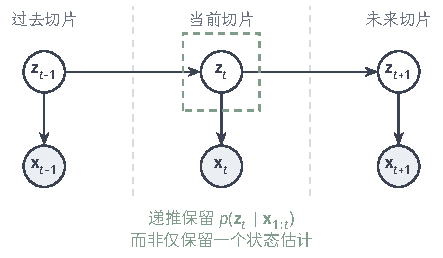
\includegraphics[width=74.997mm]{figures/06-probabilistic-graphical-models/04-models/tikz/pgm-dynamic-template/figure.pdf}
  \caption{状态空间模型在三个时刻的展开。空心节点为潜状态，填色节点为观测，竖直虚线分隔时间切片。当前潜状态的后验汇总过去证据，用于下一步预测；箭头表示生成依赖，平滑计算则沿状态链反向传递未来证据。}
  \label{fig:pgm-dynamic-template}
\end{figure}

有了联合分解，还需要说明哪些量从数据中估计。设训练集包含$N$条独立收集的序列$\bm x^{(n)}_{1:T_n}$，$\bm\theta$汇总初始、转移和观测分布中的待估参数。观测没有给出状态路径，因而每条观测序列的概率需要累加所有可能状态的贡献。参数学习的共同目标是
\begin{equation}
  \widehat{\bm\theta}\in\argmax_{\bm\theta\in\Theta}
  \ell(\bm\theta),\qquad
  \ell(\bm\theta)=\sum_{n=1}^N
  \log\int p_{\bm\theta}(\bm z_{1:T_n},\bm x^{(n)}_{1:T_n})
       \,\mathrm d\bm z_{1:T_n}.
  \label{eq:pgm-dynamic-observed-objective}
\end{equation}
其中$\Theta$要求各局部分布合法，离散状态把积分改成求和。正则或先验会改变这个目标，不能只在更新时任意加入修正。模型拟合后，状态推断是在固定参数下重新计算后验；它与对$\bm\theta$的优化是两个不同问题。

\subsection{状态记忆与跨时刻依赖}
\label{sec:pgm-dynamic-memory}

动态模型最关键的一个简化假设是：为了预测下一步，\emph{无需更早的历史}，知道当前状态就够了——更早的信息都已被当前状态“吸收”。这有点像下棋时只需知道当前棋局，而不必记住此前每一步怎么走的。递推需要保留多少历史，取决于状态怎样选择。\term{Markov假设}（Markov assumption）要求给定当前状态后，预测下一状态所需的信息已经齐备。对于$r$阶依赖$p(\bm{z}_t\mid\bm{z}_{t-r:t-1})$，可以把最近$r$个状态拼接成一个扩充状态，从而改写成一阶模型，代价是扩大状态空间。观测只间接反映内部状态，因此观测历史仍可能持续改变当前状态的后验，即使潜状态满足一阶Markov性。

设备每次按相同规则升温，温度分布仍会从冷启动逐渐向高温移动。这里保持的是局部机制：\term{时间齐次性}（time homogeneity）要求转移核不随$t$改变；\term{参数共享}（parameter sharing）表示不同位置复用同一组转移或观测参数。共享参数的条件分布若还依赖时间或已知外部输入，取值仍可随时刻变化。\term{严格平稳性}（strict stationarity）约束的则是整个过程，要求任意有限组时刻的联合分布在整体平移后保持不变。齐次Markov链从平稳分布初始化时，才得到这样的平稳过程。

将过去变量消去后，需要把哪些信息留给未来？所有跨越时间分界的依赖经过的变量集合称为\term{时间接口}（temporal interface）。一阶状态空间模型只需保留$\bm{z}_t$的后验，因为给定这个状态，过去与未来被分开。一般DBN可以保留当前切片中有下一切片子节点的变量及其联合分布。过去证据可能让这些变量相关，联合分布因此包含单独边缘没有保存的信息。计算代价取决于离散接口的联合配置数，或连续后验的表示复杂度，这也是消元中诱导宽度的重要来源（第~\ref{chap:pgm-elimination}章）。Koller和Friedman详细讨论了图模板、时间接口与精确推断的关系\scite{pgm-koller2009}。

\subsection{预测、状态重建与参数学习的接口}
\label{sec:pgm-dynamic-queries}

在进入具体模型前，先把对一条时间序列能提的几类问题区分清楚，因为它们读取证据的时间范围不同、对应不同算法：是预测\emph{未来}、估计\emph{此刻}，还是事后追溯\emph{过去}。设备监测提出三类查询。\term{预测}（prediction）给出$p(\bm{z}_{t+h}\mid\bm{x}_{1:t})$或$p(\bm{x}_{t+h}\mid\bm{x}_{1:t})$，其中$h\geq1$，用于判断未来状态或读数——此刻做决策时只允许用到目前为止的数据。\term{滤波}（filtering）给出$p(\bm{z}_t\mid\bm{x}_{1:t})$，用于\emph{在线}地、收到一个新读数就更新一次当前状态判断（像实时跟踪）。\term{平滑}（smoothing）给出$p(\bm{z}_t\mid\bm{x}_{1:T})$，其中$t<T$，用于\emph{事后}结合“未来才拿到的证据”重建过去（像检修时回看整段记录），因此通常比在线滤波判断得更准。固定间隔平滑读取长度为$T$的整段数据；固定滞后平滑只等待预定步数的未来观测，适合允许延迟的状态判断。

重建整段工况还可能需要\term{最可能状态序列}（most probable state sequence），即让$p(\bm{z}_{1:T}\mid\bm{x}_{1:T})$达到最大的整条路径。对全部潜状态求最大值得到MPE查询；保留部分状态求最大值、其余状态求和或积分，则得到边缘MAP（第~\ref{chap:pgm-elimination}章）。逐时刻取平滑边缘的最大项，对应按各位置误判数评价的决策；整条路径优化评价的是联合概率，两种目标可能选择不同结果。连续状态的路径最优以所选坐标和基准测度下的后验密度为准。

预测和滤波可以从当前后验逐步计算，平滑则在此基础上加入未来证据。记上一步滤波分布为$f_{t-1}(\bm{z}_{t-1})=p(\bm{z}_{t-1}\mid\bm{x}_{1:t-1})$。将它与转移分布结合并消去旧状态，得到当前预测；再乘当前观测似然并归一化，得到
\begin{equation}
  \begin{aligned}
    f_t^{-}(\bm{z}_t)
      &=\int p(\bm{z}_t\mid\bm{z}_{t-1})
        f_{t-1}(\bm{z}_{t-1})\,\mathrm{d}\bm{z}_{t-1},\\
    c_t
      &=\int p(\bm{x}_t\mid\bm{z}_t)
        f_t^{-}(\bm{z}_t)\,\mathrm{d}\bm{z}_t,\\
    f_t(\bm{z}_t)
      &=\frac{p(\bm{x}_t\mid\bm{z}_t)
        f_t^{-}(\bm{z}_t)}{c_t}.
  \end{aligned}
  \label{eq:pgm-dynamic-bayes-filter}
\end{equation}
第一次预测取$f_1^{-}=p(\bm{z}_1)$；每个归一化量$c_t$需有限且为正。它同时等于$c_t=p(\bm{x}_t\mid\bm{x}_{1:t-1})$，所以$\log p(\bm{x}_{1:T})=\sum_{t=1}^{T}\log c_t$给出整段观测的对数似然。一次递推因而既更新状态判断，也累计训练和模型比较需要的分数。有限状态与线性高斯模型的优势在于，这些积分或求和可以精确计算，结果仍有固定大小的表示。

\section{离散状态序列的建模与学习}
\label{sec:pgm-dynamic-discrete}

从离散状态入手最简单：状态只取有限个类别（正常/异常/故障前兆），于是“转移模型”就是一张概率表，所有求和都可以在这些有限状态上精确完成。先从最容易的情形讲起——状态能被直接看到（巡检记录了工况），这时只要数一数状态之间转移的次数就能估计转移表；再进入更常见也更难的情形——状态看不到、只有带噪观测，这时要对所有可能的隐藏路径求和。离散工况只取有限类别；其演化可以用转移概率表表示。若巡检直接记录工况，数据给出真实转移次数；若只有传感器读数，就要汇总可能的隐藏路径，再以期望次数学习。下面在这个共同问题下分别处理可见状态和隐藏状态。

\subsection{可见状态：转移结构与计数学习}
\label{sec:pgm-dynamic-visible}

如果每次巡检都能可靠记录设备的正常或异常状态，训练序列就直接给出了状态转移。用$Z_t\in\{1,\ldots,K\}$表示有限状态，$\pi_i=p(Z_1=i)$表示初始概率。齐次转移矩阵$\bm{A}\in\mathbb{R}^{K\times K}$的元素为
\[
  a_{i,j}=p(Z_t=j\mid Z_{t-1}=i),\qquad
  a_{i,j}\geq0,\quad \sum_{j=1}^{K}a_{i,j}=1.
\]
矩阵每一行列出从一个当前状态到各下一状态的概率，非负且总和为一。本节考虑有限状态、离散时间和齐次转移，初始概率$\bm\pi$按列向量记录（Markov关系参见\BookChapterRef{chap:random-variables}{卷2《数学准备：概率、因果与决策》的“随机变量”章}）。

初始概率和转移表共同定义整条可见路径的概率。训练记录为$z^{(n)}_{1:T_n}$时，本模型的结构和学习目标可明确写为
\begin{equation}
  \begin{aligned}
    p_{\bm\theta}(z_{1:T})&=\pi_{z_1}
       \prod_{t=2}^{T}a_{z_{t-1},z_t},\\
    \ell_{\mathrm{MC}}(\bm\theta)
       &=\sum_{n=1}^{N}\log\pi_{z^{(n)}_1}
           +\sum_{i,j}n_{i,j}\log a_{i,j}.
  \end{aligned}
  \label{eq:pgm-dynamic-visible-objective}
\end{equation}
这里$n_{i,j}$是所有记录内$i\to j$的总次数，$\bm\theta=(\bm\pi,\bm A)$满足概率非负和归一化约束。最大化该式就是让数据实际出现的起点与转移获得较大概率；各行归一化又防止所有转移概率同时增大。先看给定参数怎样预测，再利用同一分解求参数。

把当前状态分布记为概率列向量$\bm{q}_t$。对随机状态$Z_t$求和，下一步分布满足$\bm{q}_{t+1}=\bm{A}^{\top}\bm{q}_t$。重复这一计算便得到
\begin{equation}
  \bm{q}_{t+h}=(\bm{A}^{\top})^h\bm{q}_t,\qquad
  p(Z_{t+h}=j\mid Z_t=i)=(\bm{A}^h)_{i,j}.
  \label{eq:pgm-dynamic-markov-prediction}
\end{equation}
两步转移中的$\sum_k a_{i,k}a_{k,j}$累加了经过各个中间状态的路径概率。继续累加中间状态，就得到$h$步矩阵幂；转置来自概率列向量与按行定义的转移矩阵之间的约定。

\begin{example}[两状态设备的多步预测]
  \label{ex:pgm-dynamic-markov}
  为单独展示多步预测，设状态$1$为正常、状态$2$为异常，采用下面的人工参数。它与四节点报警模型及例~\ref{ex:pgm-sampling-filter}分别设定，后面的发射概率也将另给：
  \[
    \bm{\pi}=\begin{pmatrix}0.8\\0.2\end{pmatrix},\qquad
    \bm{A}=
    \begin{pmatrix}0.9&0.1\\0.2&0.8\end{pmatrix}.
  \]
  从确定正常的状态出发，下一步异常概率为$0.1$；两步后需要累加先正常后异常和先异常后异常两条路径，得到$0.9\times0.1+0.1\times0.8=0.17$。当前异常概率为$u_t$时，递推为
  \[
    u_{t+1}=0.1(1-u_t)+0.8u_t=0.1+0.7u_t.
  \]
  解得$u_{t+h}=1/3+0.7^h(u_t-1/3)$。初始偏差随预测步数按几何因子衰减，异常概率趋向$1/3$；这个极限由正常进入异常和异常退出两种转移共同决定。
\end{example}

例~\ref{ex:pgm-dynamic-markov}的极限是平稳分布$(2/3,1/3)^\top$，满足$\bm A^\top\bm\pi_\star=\bm\pi_\star$。平稳分布给出转移后保持不变的分布；从任意初态是否趋向它，还取决于链的长期行为条件。时间平均又涉及沿同一条路径累积的观测量，与这里的单时刻分布极限不同。下面转向如何从数据估计转移概率，以及状态隐藏时怎样推断。

可见状态的参数学习可以直接使用转移计数。令$n_{i,j}$为训练序列中$i\to j$的次数，转移对数似然为$\sum_{i,j}n_{i,j}\log a_{i,j}$。在各行总和为$1$的约束下最大化，得到$\widehat a_{i,j}=n_{i,j}/\sum_k n_{i,k}$。从未访问的行会出现$0/0$，意味着数据没有给出该行的信息，可用先验或保留旧值处理。多条独立序列分别计数后汇总，序列之间的接缝不计作转移；初始分布则只统计各序列首状态。

具体地，初始更新为$\widehat\pi_i=N^{-1}\sum_n\mathbf1\{z^{(n)}_1=i\}$。对转移表第$i$行加入乘子$\lambda_i$；正计数项的内点驻点条件为$n_{i,j}/a_{i,j}=\lambda_i$；对$j$求和并使用行和为$1$，得到$\lambda_i=\sum_jn_{i,j}$，因而产生上述计数比例，零计数项可取边界值$0$。没有隐藏变量时，这一步直接求解约束似然，无需反复运行EM。

\subsection{隐藏离散状态的组织与估计}
\label{sec:pgm-dynamic-hidden-discrete}

读数与工况并非一一对应时，我们需要同时表示工况怎样变化，以及每种工况怎样产生读数。先建立逐时刻隐藏状态模型，再分别改变它保存的历史、停留时长和内部组成。这三种变化可以组合，但每次变化都要重新确定求和的路径与学习所需统计量。

\subsubsection{HMM：逐时刻隐藏工况的学习与推断}
\label{sec:pgm-dynamic-hmm-model}

现实中真正能直接读到内部“健康工况”的情形很少，我们拿到的只是报警、温度等间接读数，而且同一个工况可能产生多种读数、同一种读数也可能来自不同工况。要描述这样的数据，需要\emph{两层}：底层是一条隐藏工况按转移表演化的Markov链，上层是“在每种工况下，读数服从什么分布”的观测机制；这就是隐马尔可夫模型——它相当于把第11章的静态混合模型加上时间轴，让前一时刻的成分影响下一时刻的成分，从而能刻画“故障会持续”而不是每刻独立乱跳。设备内部的健康状态通常隐藏在报警、温度等读数之后。用一个有限状态链描述内部演化，再给每个状态指定产生读数的分布，就得到\term{隐马尔可夫模型}（hidden Markov model, HMM）。其中的\term{发射分布}（emission distribution，这是观测模型在离散状态下的叫法，“发射”即隐藏状态把观测“发”出来）描述给定状态后的观测，记$b_j(x)=p(x\mid Z_t=j)$为它在$x$处的概率质量或密度。联合分布为
\begin{equation}
  p(z_{1:T},x_{1:T})
    =\pi_{z_1}b_{z_1}(x_1)
      \prod_{t=2}^{T}a_{z_{t-1},z_t}b_{z_t}(x_t).
  \label{eq:pgm-dynamic-hmm}
\end{equation}
HMM的隐藏状态取离散值，观测则可以是Bernoulli报警，也可以是服从状态相关高斯密度的温度。与独立混合模型相比，它用转移分布连接相邻潜类别，使前一时刻的工况影响下一时刻的成分选择（第~\ref{chap:pgm-static-directed}章）。

模型参数是$\bm\theta=(\bm\pi,\bm A,\{\bm\vartheta_j\}_{j=1}^K)$，其中$\bm\vartheta_j$控制第$j$个发射分布。训练读数仍只告诉我们$x$，不能把某条猜测的状态路径当成观测。需要最大化的目标为
\begin{equation}
  \ell_{\mathrm{HMM}}(\bm\theta)
   =\sum_{n=1}^{N}\log\sum_{z_{1:T_n}}
       \pi_{z_1}b_{z_1}(x^{(n)}_1)
       \prod_{t=2}^{T_n}a_{z_{t-1},z_t}b_{z_t}(x^{(n)}_t).
  \label{eq:pgm-dynamic-hmm-objective}
\end{equation}
求和使每条可能工况路径都按其概率贡献观测似然。后面的前向递推计算这个目标，前向--后向递推提供学习所需的期望计数，最优路径算法则只回答路径决策，三者不能互相替代。

静态混合与HMM之间还存在精确的特例关系。若所有转移行都等于同一成分比例，即$a_{i,j}=\pi_j$，起点也服从$\bm\pi$，且各时刻共享相同发射分布，则潜状态独立同分布，路径求和可以逐时刻分开，得到$\prod_t\sum_j\pi_jb_j(x_t)$。这才退回独立混合观测；仅仅让转移表对角元素较小，并不消除状态之间的依赖。

计算观测序列似然时，最笨的办法是枚举全部$K^T$条隐藏路径再相加，状态数一多就爆炸。但这些路径大量共享“前缀”：凡是在时刻$t$处于同一末状态的路径，它们后面的命运完全一样、可以合并计算。于是只需维护一个长度为$K$的消息——每个末状态对应的“所有到此前缀的概率之和”，沿时间递推即可，这正是变量消元在链上的体现。计算观测似然$p(x_{1:T})$时，直接枚举隐藏路径要遍历$K^T$个配置。具有同一末状态的前缀可以共享未来计算，因此先把它们的联合概率加在一起。这个和就是未归一化前向消息$\alpha_t(j)=p(x_{1:t},Z_t=j)$。它满足
\[
  \alpha_t(j)
    =b_j(x_t)\sum_i
      p(x_{1:t-1},Z_{t-1}=i)a_{i,j}.
\]
据此前向消息可递推为
\begin{equation}
  \begin{aligned}
    \alpha_1(j)&=\pi_jb_j(x_1),\\
    \alpha_t(j)&=b_j(x_t)\sum_{i=1}^{K}
      \alpha_{t-1}(i)a_{i,j},\\
    p(x_{1:T})&=\sum_j\alpha_T(j).
  \end{aligned}
  \label{eq:pgm-dynamic-forward}
\end{equation}
递推每次消去$Z_{t-1}$，更早路径的贡献已汇总到$\alpha_{t-1}$中。从初始联合概率出发，这一步始终保持$\alpha_t$的概率含义，也说明了前缀合并为何精确。将各状态的消息归一化，$\alpha_t(j)/\sum_i\alpha_t(i)$就是滤波概率。

前向递推只用到当前及过去的观测，给出在线滤波。事后若想更准确地重建\emph{早期}状态，还应利用“后来才观测到的证据”——连续两次报警会让我们更相信故障其实更早就在酝酿。由于链上给定$Z_t$后过去与未来条件独立，未来证据也能压缩成一条沿时间反向传播的消息，与前向消息一合并就得到平滑后验。事后重建早期状态，需要把未来证据压缩成一条反向消息。定义$\beta_t(i)=p(x_{t+1:T}\mid Z_t=i)$；末时刻没有未来观测，故$\beta_T(i)=1$。对下一状态边缘化可得
\begin{equation}
  \begin{aligned}
    \beta_t(i)&=\sum_{j=1}^{K}
      a_{i,j}b_j(x_{t+1})\beta_{t+1}(j),\\
    \gamma_t(i)&:=p(Z_t=i\mid x_{1:T})
      =\frac{\alpha_t(i)\beta_t(i)}{L},\\
    \xi_t(i,j)&:=p(Z_t=i,Z_{t+1}=j\mid x_{1:T})\\
      &=\frac{\alpha_t(i)a_{i,j}b_j(x_{t+1})
        \beta_{t+1}(j)}{L},
  \end{aligned}
  \label{eq:pgm-dynamic-backward}
\end{equation}
这里$L=p(x_{1:T})>0$为整段观测似然。给定$Z_t$后，过去与未来观测条件独立，因而$\alpha_t\beta_t$可以合并两部分证据，再由同一个似然归一化。\term{前向--后向算法}（forward--backward algorithm）据此分别压缩过去和未来：$\gamma_t$给出单时刻平滑，$\xi_t$保存相邻状态的联合后验，供转移参数学习使用。

为减少长序列连乘造成的数值下溢，每一步都把前向消息归一化，记$\widehat\alpha_t(j)=p(Z_t=j\mid x_{1:t})$，并保存未归一化消息的总和$c_t$。后向缩放与它配合：令$\widehat\beta_T=1$，将$\sum_j a_{i,j}b_j(x_{t+1})\widehat\beta_{t+1}(j)$除以$c_{t+1}$。这样$\gamma_t(i)=\widehat\alpha_t(i)\widehat\beta_t(i)$，$\xi_t$也使用$c_{t+1}$归一化。另一种实现是在对数域稳定求和。若$c_t=0$，当前观测前缀落在模型支撑之外，应终止更新并检查分布设定或数值计算。

\begin{algorithm}[缩放的HMM前向--后向递推]
  \label{alg:pgm-dynamic-forward-backward}
  \begin{algorithmic}[1]
    \Require $\bm{\pi},\bm{A},b_j$与观测$x_{1:T}$，$T\geq1$
    \Ensure 似然对数、平滑概率$\gamma_t$与成对概率$\xi_t$
    \State $u_1(j)\gets\pi_jb_j(x_1)$，$c_1\gets\sum_j u_1(j)$
    \State 若$c_1=0$，报告观测不在模型支撑内并终止
    \State $\widehat\alpha_1(j)\gets u_1(j)/c_1$
    \For{$t=2,\ldots,T$}
      \State $u_t(j)\gets b_j(x_t)\sum_i\widehat\alpha_{t-1}(i)a_{i,j}$
      \State $c_t\gets\sum_j u_t(j)$；若$c_t=0$则报告并终止
      \State $\widehat\alpha_t(j)\gets u_t(j)/c_t$
    \EndFor
    \State $\widehat\beta_T(i)\gets1$，$\gamma_T(i)\gets\widehat\alpha_T(i)$
    \For{$t=T-1,\ldots,1$}
      \State $\widehat\beta_t(i)\gets
        \sum_j a_{i,j}b_j(x_{t+1})\widehat\beta_{t+1}(j)/c_{t+1}$
      \State $\gamma_t(i)\gets\widehat\alpha_t(i)\widehat\beta_t(i)$
      \State $\xi_t(i,j)\gets
        \widehat\alpha_t(i)a_{i,j}b_j(x_{t+1})
        \widehat\beta_{t+1}(j)/c_{t+1}$
    \EndFor
    \State 返回$\sum_t\log c_t$及上述后验统计量
  \end{algorithmic}
\end{algorithm}

密集转移下，算法~\ref{alg:pgm-dynamic-forward-backward}每步遍历状态对，时间成本为$O(TK^2)$，再加发射概率求值。在线滤波只保留一条消息，工作内存为$O(K)$；平滑保存全部前向消息，需要$O(TK)$内存。为EM计算转移计数时，可以逐步累加$\xi_t$，省去$T$张$K\times K$表的存储。若转移图稀疏，计算只遍历允许的边，成本随这些边的数量变化。

\begin{example}[报警证据怎样改变过去的判断]
  \label{ex:pgm-dynamic-hmm}
  沿用例~\ref{ex:pgm-dynamic-markov}的$\bm{\pi}$和$\bm{A}$。记$X_t=1$为报警，另设教学发射概率$b_1(1)=0.1$、$b_2(1)=0.7$，表示异常工况更易报警。观测$x_{1:3}=(0,1,1)$产生如下前向消息：
  \[
    \begin{aligned}
      \bm{\alpha}_1&=(0.72,0.06)^\top,\\
      \bm{\alpha}_2&=(0.066,0.084)^\top,\\
      \bm{\alpha}_3&=(0.00762,0.05166)^\top.
    \end{aligned}
  \]
  第二步的正常权重为$(0.72\times0.9+0.06\times0.2)\times0.1=0.066$：先汇总两种前状态转到正常的贡献，再乘正常时报警的概率。总似然为$0.05928$，后向消息依次为$\bm{\beta}_3=(1,1)^\top$、$\bm{\beta}_2=(0.16,0.58)^\top$和$\bm{\beta}_1=(0.055,0.328)^\top$。第一个时刻的异常滤波概率是$0.06/0.78\approx0.0769$，加入后续证据后的异常平滑概率为$0.06\times0.328/0.05928\approx0.3320$。连续报警增加了此前已经异常、第一次却未报警这一解释的权重。
\end{example}

表~\ref{tab:pgm-dynamic-hmm-example}把同一序列的两类判断并列。这里，两次报警及异常状态的持续性共同提高了早期异常的后验概率；在其他观测序列下，未来证据也可以降低这个概率。

\begin{table}[htbp]
  \centering
  \begin{tabular}{ccrr}
    \toprule
    时刻$t$ & 报警$x_t$ & 异常滤波概率 & 异常平滑概率 \\
    \midrule
    $1$ & $0$ & $0.076923$ & $0.331984$ \\
    $2$ & $1$ & $0.560000$ & $0.821862$ \\
    $3$ & $1$ & $0.871457$ & $0.871457$ \\
    \bottomrule
  \end{tabular}
  \caption{同一人工设备序列的异常后验。滤波列逐步读取当前及过去观测，平滑列使用完整$x_{1:3}$；最后一个时刻的证据范围相同，因而两列重合。}
  \label{tab:pgm-dynamic-hmm-example}
\end{table}

前面求的是各时刻状态的边缘分布，回答“此刻最可能是什么状态”；但很多问题要的是\emph{整条最可能的状态路径}（如最可能的完整故障过程）。注意“逐时刻各自取最可能”与“整条联合最可能”并不等价，后者必须考虑相邻状态的转移相容性。求最优路径仍可动态规划：由于最优路径经过时刻$t$的某个状态后，其前缀必定也是到达该状态的最优前缀，每个末状态只需保留一个最优前缀和它的前驱，逐步递推到末端再回溯即可。寻找联合概率最大的路径时，每个末状态只需保留最优前缀及其前驱。记$\delta_t(j)$为以$j$结尾的路径中最大的联合概率$p(z_{1:t},x_{1:t})$，用前驱表保存最大值来自哪一个状态。\term{Viterbi算法}（Viterbi algorithm）据此递推：
\begin{equation}
  \begin{aligned}
    \delta_1(j)&=\pi_jb_j(x_1),\\
    \delta_t(j)&=b_j(x_t)\max_i
      \{\delta_{t-1}(i)a_{i,j}\},\\
    \psi_t(j)&\in\argmax_i
      \{\delta_{t-1}(i)a_{i,j}\}.
  \end{aligned}
  \label{eq:pgm-dynamic-viterbi}
\end{equation}
先选末状态$z_T^\star\in\argmax_j\delta_T(j)$，再按$z_t^\star=\psi_{t+1}(z_{t+1}^\star)$回溯；平局可按最小索引处理。当末状态固定时，未来因子对全部前缀相同，所以保留较优前缀足以保留整体最优解。密集转移的时间成本仍为$O(TK^2)$，回溯表占$O(TK)$。对数得分实现可避免路径概率连乘下溢，并以$-\infty$表示禁止的转移。

例~\ref{ex:pgm-dynamic-hmm}的最优路径是$(1,2,2)$，联合概率为$0.8\times0.9\times0.1\times0.7\times0.8\times0.7=0.028224$，给定观测后的路径概率约为$0.4761$，其余概率仍分散在其他路径上。逐位置选择与联合选择的差别可看另一个两时刻分布：令$(1,1),(1,2),(2,1),(2,2)$的概率为$0.40,0.25,0.01,0.34$，两个边缘分别选择$1$和$2$，组成的$(1,2)$却不如联合最优$(1,1)$。取初始分布$(0.65,0.35)$并按上述联合概率确定条件转移，即可构造这个Markov例子。

可见Markov链学参数靠数真实转移次数；HMM里状态隐藏，真实计数拿不到。沿用第9章EM的思路：不把状态路径硬猜成某一条，而是按当前参数算出每条相邻转移、每个状态在各时刻的\emph{后验概率}，用这些软计数充当期望次数，再像可见链一样按比例更新参数，如此交替。隐藏状态没有实际可读的转移计数，却可以按各路径的后验概率累计期望计数。\term{Baum--Welch算法}（Baum--Welch algorithm）用这一思路在HMM上执行EM：E步计算当前参数下的$\gamma_t,\xi_t$，M步根据这些软计数拟合初始、转移和发射分布。当前参数记为$\bm{\theta}^{(k)}$，期望完全数据对数似然为
\begin{equation}
  \begin{aligned}
    \mathcal{Q}(\bm{\theta}\mid\bm{\theta}^{(k)})
      &=\sum_i\gamma_1(i)\log\pi_i\\
      &\quad{}+\sum_{t=1}^{T-1}\sum_{i,j}
        \xi_t(i,j)\log a_{i,j}\\
      &\quad{}+\sum_{t=1}^{T}\sum_j
        \gamma_t(j)\log b_j(x_t).
  \end{aligned}
  \label{eq:pgm-dynamic-hmm-em-objective}
\end{equation}
在一次M步中固定旧参数算出的后验权重，只调整对数内的候选参数。对$a_{i,j}$施加逐行归一化约束，一阶条件给出$a_{i,j}\propto\sum_t\xi_t(i,j)$。由于$\sum_j\xi_t(i,j)=\gamma_t(i)$，更新可写为
\begin{equation}
  \begin{aligned}
    \pi_i^{(k+1)}&=\gamma_1(i),\\
    a_{i,j}^{(k+1)}
      &=\frac{\sum_{t=1}^{T-1}\xi_t(i,j)}
        {\sum_{t=1}^{T-1}\gamma_t(i)},\\
    b_j^{(k+1)}(v)
      &=\frac{\sum_{t=1}^{T}
        \gamma_t(j)\mathbf{1}\{x_t=v\}}
        {\sum_{t=1}^{T}\gamma_t(j)}.
  \end{aligned}
  \label{eq:pgm-dynamic-baum-welch}
\end{equation}
类别发射用最后一行的期望频数更新。高斯发射则按$\sum_t\gamma_t(j)\bm{x}_t/\sum_t\gamma_t(j)$更新均值，再围绕这个新均值累计加权残差外积，得到协方差。多条独立序列先分别计算统计量，再相加更新转移和发射；初始概率使用各序列$\gamma_1$的平均。

本例得到$\xi_1(1,2)=0.72\times0.1\times0.7\times0.58/0.05928\approx0.493117$和$\xi_2(1,2)\approx0.077935$。一次M步将$a_{1,2}$更新为$(0.493117+0.077935)/(0.668016+0.178138)\approx0.674880$，两个状态的报警概率变为$0.314642$和$0.836082$。只有三次读数时，估计容易随证据显著变化。训练中可比较多组初值，用似然相对增量与迭代上限控制停止，再用独立序列或时间隔离的验证段评价这些参数的预测表现。

精确E步与提高$\mathcal Q$的M步使观测似然单调不降（第~\ref{chap:pgm-parameter-learning}章），它评价的是同一训练数据上的目标进展。全局最优需要进一步的优化条件，状态解释依赖可识别性，测试预测则需要独立数据检验。某个更新分母为零时，该轮后验没有访问相应状态，软计数对参数不提供信息。正初始化、结构约束和先验可以处理部分退化，估计的可识别范围仍由数据与模型共同决定。

给隐藏状态重新编号，同时置换$\bm{\pi}$、$\bm{A}$的行列和对应发射分布，会得到完全相同的观测似然。这种\term{标签交换}（label switching）使状态编号只能在选定约定下解释。发射分布接近时，数据也难以区分状态；全部发射相同且按式~\eqref{eq:pgm-dynamic-hmm}生成时，状态路径求和后，观测分布中的转移信息完全消失。选择状态数$K$时，增加$K$可能复制已有状态，也可能补偿持续时间假设的偏差。应结合验证预测似然、持续时间解释和后验占用检查模型；使用常规信息准则还需考虑潜变量模型的奇异性与可识别性条件。Murphy的教材系统介绍了HMM推断、学习和模型选择\scite{pgm-murphy2012}。

普通HMM用当前类别概括历史，又以自转移决定停留时间。若当前类别不足以区分近期经历、设备对持续时长有额外约束，或者多个内部过程共同影响读数，就需要改变相应结构。以下三个子小节分别处理这些不同缺口；它们不是按性能高低排列的替代方案。

\subsubsection{高阶HMM：用扩充状态保存有限历史}
\label{sec:pgm-dynamic-higher-order}

一阶Markov假设“知道当前状态就够了”有时过强：设备下一时刻是否退出异常，可能取决于它已经连续异常了多久、或最近几步的具体经过。若下一状态确实依赖最近$r$个状态，可以直接把这$r$个状态\emph{拼接成一个更大的扩充状态}，从而在形式上仍是一阶模型——代价是状态数从$K$膨胀到$K^r$。实际系统可能需要更长历史来预测转移。若下一状态依赖最近$r$个状态，模型成为\term{高阶HMM}（higher-order HMM）。把$(Z_{t-r+1},\ldots,Z_t)$拼成扩充状态后，仍可执行动态规划。一次转移移去最早状态、加入新状态，所以每个扩充状态只有$K$个合法后继，计算成本为$O(TK^{r+1})$。虽然共有$K^r$个扩充状态，转移图保留了稀疏移位结构；消息本身仍需记录$K^r$个配置。

仅说明扩充状态还没有完全定义模型。令$\rho(z_{1:r})$为起点联合分布，$a_{u,j}$为历史上下文$u\in\{1,\ldots,K\}^r$之后的转移概率，保留当前状态的发射$b_j$。当$T\geq r$时，结构与学习目标为
\begin{equation}
  \begin{aligned}
    p_{\bm\theta}(z,x)&=\rho(z_{1:r})
       \prod_{t=r+1}^{T}a_{z_{t-r:t-1},z_t}
       \prod_{t=1}^{T}b_{z_t}(x_t),\\
    \ell_r(\bm\theta)&=\sum_n\log\sum_{z_{1:T_n}}
                       p_{\bm\theta}(z,x^{(n)}).
  \end{aligned}
  \label{eq:pgm-dynamic-higher-objective}
\end{equation}
短于$r$的序列使用$\rho$的相应起点边缘。学习先在合法移位图上运行前向--后向，累计“上下文$u$后接$j$”的后验期望次数$N_{u,j}$，再按$a_{u,j}^{\mathrm{new}}=N_{u,j}/\sum_kN_{u,k}$更新；发射参数仍使用当前状态的后验边缘。起点统计来自各独立序列的初始状态块，不能把不同记录连接起来。上下文未获得后验占用时，该行仍没有可估信息。扩充状态是计算表示，任意放开其稠密转移会改变原来的高阶模型。

\subsubsection{隐半Markov模型：显式学习状态持续时间}
\label{sec:pgm-dynamic-hsmm-model}

普通HMM对“在一个状态停留多久”只有一个隐含的、很受限的描述：每一步都以固定的自转移概率决定是否留下，于是停留时长被迫服从几何分布，其特点是“刚进入就离开”的概率最高、已停留越久的条件退出风险并不累积，这与很多实际设备（至少要运行若干步、或老化后更易退出）不符。要如实刻画持续时长，应把“这一片段持续多久”显式建模成一个随机变量。设备在一种工况中已经运行的时长，也可能影响退出概率。普通HMM进入状态$i$后，每步以固定概率$a_{i,i}<1$继续停留，因此连续停留时长$D$服从
\begin{equation}
  p(D=\ell\mid i)=(a_{i,i})^{\ell-1}(1-a_{i,i}),
  \qquad
  \mathbb{E}[D\mid i]=\frac{1}{1-a_{i,i}}.
  \label{eq:pgm-dynamic-geometric-duration}
\end{equation}
其中$\ell-1$次自转移后接一次退出，产生\term{几何持续时间}（geometric duration）。退出概率与已经停留的时长无关，本例正常工况的平均持续时间为$10$步。如果设备必须运行至少$5$步才允许退出，就需要让持续时间本身进入模型。

为工况另给持续时间分布$g_j(\ell)$，得到\term{显式持续时间模型}（explicit-duration model）。\term{隐半Markov模型}（hidden semi-Markov model, HSMM）据此以片段为单位：片段内部状态固定，边界处按$\widetilde a_{i,j}$转移。常用$\widetilde a_{j,j}=0$使相邻片段对应不同状态。状态$j$的片段长$\ell$、结束于$t$时，条件观测似然为$B_j(t,\ell)=\prod_{s=t-\ell+1}^{t}b_j(x_s)$。这里假设序列从新片段开始，$g_j$在$\{1,\ldots,D_{\max}\}$上归一化。记$F_t(j)$为观测前缀与一个$j$片段恰在$t$结束的联合概率，$G_s(j)$为前$s$步观测与下一片段进入$j$的联合权重，递推为
\begin{equation}
  \begin{aligned}
    G_0(j)&=\pi_j,\\
    G_s(j)&=\sum_{i\ne j}
      F_s(i)\widetilde a_{i,j},\qquad s\geq1,\\
    F_t(j)&=\sum_{\ell=1}^{\min(t,D_{\max})}
      g_j(\ell)B_j(t,\ell)G_{t-\ell}(j).
  \end{aligned}
  \label{eq:pgm-dynamic-hsmm}
\end{equation}
每一项把前一片段的权重、当前片段的长度概率和观测似然相乘，再对可能长度求和。采样固定在$T$停止时，最后一段可能仍在持续，形成右删失。用存活概率$\overline g_j(\ell)=p(D\geq\ell\mid j)$保留这一信息，整体似然为
\[
  p(x_{1:T})=\sum_j\sum_{\ell=1}^{\min(T,D_{\max})}
    \overline g_j(\ell)B_j(T,\ell)G_{T-\ell}(j).
\]
这一式子包含在$T$结束和越过终点继续持续的片段。若采样也从片段中途开始，需另外指定初始剩余时长分布。预计算片段发射概率并缓存$G_s(j)$后，常规成本从$O(TD_{\max}K^2)$降到$O(TK^2+TD_{\max}K)$，其中先汇总边界转移，再枚举片段长度；这一分离依赖发射条件独立及持续时间不依赖前驱状态。将无限支撑持续时间截断会引入额外误差。EM相应累计片段、边界转移和持续时间的后验期望计数。

为了把这个过程用于训练，令$\mathcal S_T$表示在当前起止约定下允许的潜片段配置，$s$记录片段状态、边界、完整片段的时长以及末段已观察的长度；末段尚未观察的剩余长度已由存活概率求和。其权重由初态、边界转移、完整片段长度概率和发射相乘；固定终点处尚未结束的片段用上述存活项。于是本模型的观测目标是
\begin{equation}
  \ell_{\mathrm{HSMM}}(\bm\theta)
    =\sum_{n=1}^{N}\log\sum_{s\in\mathcal S_{T_n}}
            p_{\bm\theta}(s,x^{(n)}),
  \label{eq:pgm-dynamic-hsmm-objective}
\end{equation}
其中$\bm\theta$包括初态、$\widetilde{\bm A}$、$g_j$和发射参数。E步在边界与时长递推中计算片段及相邻片段的后验概率。M步将边界期望次数按出发状态归一化，更新$\widetilde{\bm A}$；再由各位置属于状态$j$的后验概率更新发射。若使用有限表表示$g_j$，可以把被删失片段的未观测完整长度也纳入E步，再按完整长度的期望频数归一化；若直接优化存活似然，必须保留$\log\overline g_j$的贡献。把末段已观察长度当成真实结束长度，会系统改变时长目标。

要与普通HMM精确对应，需要将时长支撑扩展为全部正整数。在从新片段开始、片段间不自转移的口径下，取$g_i(d)=a_{i,i}^{d-1}(1-a_{i,i})$及$\widetilde a_{i,j}=a_{i,j}/(1-a_{i,i})$（$j\ne i$且$a_{i,i}<1$），并匹配终点删失处理，HSMM可以重现相应HMM的状态路径分布；有限截断的时长表一般不能保留这一全分布等价。显式时长因此改变的是停留机制；它不自动意味着每一组数据上的预测都会改善。

\subsubsection{因子HMM：多条状态链通过观测相互解释}
\label{sec:pgm-dynamic-factorial-model}

到目前为止都用\emph{一条}隐藏状态链概括全部内部过程。但系统里可能并行着多个相对独立的内部过程——设备本身的健康在演化、传感器自身的工作状态也在演化，两者共同决定最终报警。若硬塞进一条链，状态数会变成各过程状态的笛卡尔积、组合爆炸。更贴切的是用\emph{多条}各自转移、只在产生观测时才耦合的隐藏链。设备健康状态和传感器工作状态也可能分别演化，却共同决定报警。\term{因子HMM}（factorial HMM）用多条隐藏链表示这些过程。记$Z_{t,m}$为第$m$条链的状态，$m=1,\ldots,M$，模型规定
\begin{equation}
  \begin{aligned}
    p(\bm{z}_t\mid\bm{z}_{t-1})
      &=\prod_{m=1}^{M}
        p(z_{t,m}\mid z_{t-1,m}),\\
    p(\bm{x}_t\mid\bm{z}_t)
      &=p(\bm{x}_t\mid z_{t,1},\ldots,z_{t,M}).
  \end{aligned}
  \label{eq:pgm-dynamic-factorial}
\end{equation}
先验转移分别作用于各条链，共同观测则把它们连接起来。

若还指定分解初态$\prod_m\pi^{(m)}_{z_{1,m}}$，完整联合结构和观测学习目标就是
\begin{equation}
  \begin{aligned}
    p_{\bm\theta}(z,x)
      &=\prod_m\pi^{(m)}_{z_{1,m}}
        \prod_{t=2}^{T}\prod_m a^{(m)}_{z_{t-1,m},z_{t,m}}
        \prod_{t=1}^{T}p_{\bm\theta}(x_t\mid z_{t,1:M}),\\
    \ell_{\mathrm{FHMM}}(\bm\theta)
      &=\sum_n\log\sum_{z_{1:T_n,1:M}}
                            p_{\bm\theta}(z,x^{(n)}).
  \end{aligned}
  \label{eq:pgm-dynamic-factorial-objective}
\end{equation}
这里先验链独立需要初态与转移都按链分解；它不是仅凭转移式就能推出的结论。每条链表示一个内部过程，共同发射则规定这些过程怎样一起产生读数。例如，同一次报警可以由设备异常或传感器异常解释，观测后两种解释的概率彼此关联。每链$K$个状态时，精确联合消息包含$K^M$种配置；按各维依次收缩转移乘积，可用约$O(MK^{M+1})$成本完成一步预测，仍随链数指数增长。结构化变分保留链内时间依赖并近似链间相关，采样也可以估计E步统计量。Ghahramani和Jordan系统分析了因子HMM的这种后验耦合\scite{pgm-dynamic-ghahramani1997}。

因子HMM的E步计算共同观测下的联合后验，再取各链的相邻状态边缘。令$N^{(m)}_{i,j}$为第$m$条链从$i$转到$j$的后验期望总次数，M步按$a^{(m),\mathrm{new}}_{i,j}=N^{(m)}_{i,j}/\sum_kN^{(m)}_{i,k}$更新该链转移，初态使用各序列起点边缘的平均。共同发射参数则最大化$\sum_{n,t}\mathbb E[\log p_{\bm\vartheta}(x_t^{(n)}\mid Z_{t,1:M})\mid x^{(n)}]$，其统计量由所选发射参数化决定，不能只保留各链单独的边缘就任意分开更新。变分或采样E步改变的是这些期望的计算，近似精度与原似然的进展要分别检查。

把所有链合为一个大状态，可以将它表示为状态数至多$K^M$的HMM，但转移与发射带有原来的分解约束。任意大状态HMM通常没有这组约束。第~\ref{sec:pgm-dynamic-undirected-factorial-crf}节的多状态链条件模型也保留多个输出，却直接建模给定输入后的标签分布，不承担这里的观测生成任务。

\section{连续状态序列的建模与学习}
\label{sec:pgm-dynamic-continuous}

离散HMM用有限状态格子近似真实状态，想要的分辨率越高、状态数$K$就越大，转移表和计算量随之膨胀，而且离散化本身会丢失状态间“距离”的信息（温度30度和31度比30度和90度更接近，在类别标签里却看不出来）。对温度、位置、速度这类本质连续的状态，更自然的是直接在连续空间里建模；这时求和变成积分，后验能否用有限参数精确保存，取决于转移和观测函数的形式——当它们都是线性加高斯噪声时，后验始终是高斯，只需要递推均值和协方差两个量。当状态表示温度、位置或强度时，连续量比有限工况更直接。此时求和变成积分，能否用有限参数精确保存后验，取决于转移和观测机制。线性高斯模型先展示积分闭合的情形；随后的一般连续模型说明哪些计算需要近似。

\subsection{线性高斯状态空间模型的推断与学习}
\label{sec:pgm-dynamic-lgssm-model}

连续状态空间里什么情况下递推能精确闭合？关键在于：高斯分布经线性变换仍是高斯、两个高斯相乘（条件化）仍是高斯。因此若初始状态是高斯、状态按线性方程加高斯噪声演化、观测是状态的线性函数加高斯噪声，那么滤波、平滑的后验在每一时刻都还是高斯，永远只需维护均值向量和协方差矩阵即可完整描述，这就是Kalman滤波的情形。温度偏移和位置需要连续数值表示；若用有限状态格子追踪，分辨率越高，HMM的状态数越大。保留连续状态后，还可以借助高斯族完成精确递推：线性变换和高斯条件化都保持高斯形式。\term{线性高斯状态空间模型}（linear Gaussian state space model, LGSSM）采用高斯初态、线性映射和独立高斯扰动，使整个有限序列成为联合高斯。

设潜状态$\bm{z}_t\in\mathbb{R}^{q}$、观测$\bm{x}_t\in\mathbb{R}^{p}$。对于齐次参数且无外部输入的系统，基本方程为
\begin{equation}
  \begin{aligned}
    \bm{z}_1&\sim\mathcal{N}(\bm{m}_0,\bm{P}_0),\\
    \bm{z}_t&=\bm{A}\bm{z}_{t-1}+\bm{\varepsilon}_t,
      &\bm{\varepsilon}_t&\sim\mathcal{N}(\bm{0},\bm{Q}),\\
    \bm{x}_t&=\bm{C}\bm{z}_t+\bm{\eta}_t,
      &\bm{\eta}_t&\sim\mathcal{N}(\bm{0},\bm{R}).
  \end{aligned}
  \label{eq:pgm-dynamic-lgssm}
\end{equation}
矩阵$\bm{A}\in\mathbb{R}^{q\times q}$作用于状态，$\bm{C}\in\mathbb{R}^{p\times q}$把状态映射为观测均值；$\bm{Q}$、$\bm{R}$分别描述过程和测量噪声。噪声相互独立、跨时刻独立，并与初始状态独立。这里$\bm{A}$是线性映射，其行和可以偏离$1$，与离散转移表的含义不同。先取$\bm{P}_0,\bm{Q},\bm{R}$正定，以便使用密度和逆矩阵；退化情形需在支撑子空间内处理。已知控制量$\bm{u}_t$可以通过$\bm{B}\bm{u}_t$进入状态方程，时变矩阵也可按时刻递推，保留的是线性高斯结构。

这一模型要学习的量是$\bm\theta=(\bm m_0,\bm P_0,\bm A,\bm C,\bm Q,\bm R)$，不是每个时刻的一条确定状态轨迹。对于独立观测序列，目标明确为
\begin{equation}
  \widehat{\bm\theta}\in\argmax_{\bm\theta\in\Theta_{\mathrm{LG}}}
    \sum_{n=1}^{N}\log p_{\bm\theta}(\bm x^{(n)}_{1:T_n}),
  \label{eq:pgm-dynamic-lgssm-objective}
\end{equation}
其中$\Theta_{\mathrm{LG}}$包含所选维度、协方差正定性与需要的结构约束。下面的滤波给出精确观测似然，平滑提供EM所需矩，M步再更新这些参数。

与静态因子模型相比，这里让连续潜因素通过$\bm A$跨时刻联系。对于已中心化观测，在$q<p$的低维设定下，若取$\bm A=0$、$\bm Q=\bm P_0=\bm I$、$\bm m_0=0$，并把$\bm R$约束为对角矩阵，则各状态独立服从标准高斯，每个位置就是以$\bm C$为载荷的因子分析；再令$\bm R=\sigma^2\bm I$便得到对应的概率主成分模型。一般LGSSM不具有这些独立与噪声约束，故不能仅把状态叫作“因子”就认定二者相同。这一关系也解释了学习统计为何从静态的一二阶矩增加到相邻状态的联合矩。

用$\bm{m}_{t\mid s}=\mathbb{E}[\bm{z}_t\mid\bm{x}_{1:s}]$和$\bm{P}_{t\mid s}=\operatorname{Cov}(\bm{z}_t\mid\bm{x}_{1:s})$记录后验均值和协方差。在上述线性高斯条件下，这两项完整确定状态后验（相关状态估计基础可参考\BookChapterRef{chap:dynamical-systems-and-state-estimation}{卷2《数学准备：概率、因果与决策》的“动力系统与状态估计”章}）。对本章的状态和观测$\bm z_t,\bm x_t$，先将旧滤波分布经线性转移传播，得到
\begin{equation}
  \begin{aligned}
    \bm{m}_{t\mid t-1}&=\bm{A}\bm{m}_{t-1\mid t-1},\\
    \bm{P}_{t\mid t-1}
      &=\bm{A}\bm{P}_{t-1\mid t-1}\bm{A}^{\top}
        +\bm{Q}.
  \end{aligned}
  \label{eq:pgm-dynamic-kalman-predict}
\end{equation}
起点$t=1$使用给定初始分布，即$\bm{m}_{1\mid0}=\bm{m}_0$、$\bm{P}_{1\mid0}=\bm{P}_0$。此后的预测协方差把两种来源相加：旧状态的不确定性经过线性映射传播，过程噪声贡献本步新增的不确定性。

预测观测的协方差为$\bm S_t=\bm C\bm P_{t\mid t-1}\bm C^\top+\bm R$。实际读数与预测均值之差称为新息，对状态与观测的联合高斯分布作条件化，得到
\begin{equation}
  \begin{aligned}
    \bm{e}_t&=\bm{x}_t-\bm{C}\bm{m}_{t\mid t-1},\\
    \bm{K}_t&=\bm{P}_{t\mid t-1}\bm{C}^{\top}\bm{S}_t^{-1},\\
    \bm{m}_{t\mid t}
      &=\bm{m}_{t\mid t-1}+\bm{K}_t\bm{e}_t,\\
    \bm{P}_{t\mid t}
      &=\bm{P}_{t\mid t-1}
        -\bm{K}_t\bm{S}_t\bm{K}_t^{\top}.
  \end{aligned}
  \label{eq:pgm-dynamic-kalman-update}
\end{equation}
新息$\bm e_t$给出测量与预测的偏差，Kalman增益$\bm K_t$把这个偏差转成状态均值的修正。在线性高斯及独立噪声条件下，更新给出精确后验；仅有二阶矩时，它可用于最佳线性估计，一般非高斯后验的完整形状还需要其他信息。实现增益时可解线性方程，协方差则可用Joseph形式或平方根递推保持数值稳定；前者把更新写成两个半正定项之和，后者直接维护协方差的因子。缺失机制可忽略时，无观测的一步只做预测，部分缺失则取$\bm C$的实际观测行与$\bm R$的相应子矩阵；可忽略条件见第~\ref{chap:pgm-parameter-learning}章。

同一个预测计算给出观测密度$\mathcal N(\bm{x}_t;\bm{C}\bm{m}_{t\mid t-1},\bm{S}_t)$。把各步预测密度的对数累加，得到
\begin{equation}
  \log p(\bm{x}_{1:T})
    =-\frac12\sum_{t=1}^{T}
      \left[
        p\log(2\pi)+\log|\bm{S}_t|
        +\bm{e}_t^\top\bm{S}_t^{-1}\bm{e}_t
      \right].
  \label{eq:pgm-dynamic-kalman-likelihood}
\end{equation}
对数似然同时衡量预测偏差和预测不确定性，可用于拟合参数与评价观测预测。完整观测、密集矩阵下，每步常规成本为$O(q^3+p^3+q^2p+qp^2)$；在线状态存储为$O(q^2)$，观测计算另外需要约$p^2+pq$大小的矩阵。状态与观测维度固定时，总成本随序列长度$T$线性增加。

学习参数需要整段观测下的状态矩，因此在前向滤波之后反向传播未来证据。Rauch--Tung--Striebel（RTS）平滑用下面的增益，将下一状态的平滑修正传回当前状态：
\[
  \bm{J}_t=\bm{P}_{t\mid t}\bm{A}^{\top}
    \bm{P}_{t+1\mid t}^{-1}.
\]
在线性高斯条件下，反向条件均值及协方差给出精确递推：
\begin{equation}
  \begin{aligned}
    \bm{m}_{t\mid T}
      &=\bm{m}_{t\mid t}
        +\bm{J}_t(\bm{m}_{t+1\mid T}
          -\bm{m}_{t+1\mid t}),\\
    \bm{P}_{t\mid T}
      &=\bm{P}_{t\mid t}
        +\bm{J}_t(\bm{P}_{t+1\mid T}
          -\bm{P}_{t+1\mid t})\bm{J}_t^\top.
  \end{aligned}
  \label{eq:pgm-dynamic-rts}
\end{equation}
从$t=T$的滤波结果初始化，依次处理$t=T-1,\ldots,1$，便得到各时刻给定整段观测的平滑均值及协方差。逆向增益使用前向滤波协方差，因而未来证据沿各时刻已建立的条件关系传回。保存前向均值、协方差和预测量后，常规实现需$O(Tq^2)$存储，反向过程增加$O(Tq^3)$的密集矩阵计算。

学习转移映射还需要相邻状态的联合矩。反向条件均值的残差与$\bm{z}_{t+1}$条件不相关，所以其滞后一阶协方差为
\begin{equation}
  \begin{aligned}
    \bm{P}_{t,t-1\mid T}
      &:=\operatorname{Cov}(\bm{z}_t,\bm{z}_{t-1}
        \mid\bm{x}_{1:T})\\
      &=\bm{P}_{t\mid T}\bm{J}_{t-1}^{\top},
      \qquad t=2,\ldots,T.
  \end{aligned}
  \label{eq:pgm-dynamic-lag-covariance}
\end{equation}
转置决定这里的方向：$\bm{J}_{t-1}\bm{P}_{t\mid T}$给出$\operatorname{Cov}(\bm{z}_{t-1},\bm{z}_{t}\mid\bm{x}_{1:T})$，与展示式互为转置。相邻状态仍共享后验不确定性，学习动态关系时，需要把这项协方差与均值外积一起计入。

\begin{example}[温度偏移的滤波、平滑与二阶矩]
  \label{ex:pgm-dynamic-kalman}
  另设一个以摄氏度为单位的人工温度偏移模型：$Z_1\sim\mathcal{N}(0,1)$、$Z_2=Z_1+\varepsilon_2$、$X_t=Z_t+\eta_t$，两类噪声独立且均为$\mathcal{N}(0,1)$，方差单位是摄氏度平方。读数$x_1=1,x_2=2$到来后，首次滤波得到$K_1=1/2$、$m_{1\mid1}=0.5$、$P_{1\mid1}=0.5$。第二步预测保留均值$m_{2\mid1}=0.5$，过程噪声把方差增至$P_{2\mid1}=1.5$。增益$K_2=1.5/2.5=0.6$将新读数融入预测，得到
  \[
    m_{2\mid2}=0.5+0.6(2-0.5)=1.4,\qquad
    P_{2\mid2}=0.6.
  \]
  反向使用平滑增益$J_1=0.5/1.5=1/3$，得到
  \[
    \begin{aligned}
      m_{1\mid2}&=0.5+(1/3)(1.4-0.5)=0.8,\\
      P_{1\mid2}&=0.5+(1/3)^2(0.6-1.5)=0.4,\\
      P_{2,1\mid2}&=0.6/3=0.2.
    \end{aligned}
  \]
  第二次观测使早期状态均值从$0.5$修正为$0.8$，修正幅度由状态间的关系决定，读数$2$只提供间接证据。联合平滑协方差$\bigl(\begin{smallmatrix}0.4&0.2\\0.2&0.6\end{smallmatrix}\bigr)$的非零非对角项记录了两个状态共享的不确定性。
\end{example}

图~\ref{fig:pgm-dynamic-kalman-trajectory}将同样的递推用于二维位置，采用随机游走$\bm z_t=\bm z_{t-1}+\bm\varepsilon_t$和直接观测$\bm x_t=\bm z_t+\bm\eta_t$，参数固定为$\bm Q=\operatorname{diag}(0.8,0.5)$、$\bm R=\operatorname{diag}(0.45,0.3)$及$\bm P_0=0.4\bm I$。该图的九次观测从零开始编号。随机游走的一步预测均值延续上一滤波位置，在图中持续移动的轨迹上出现滞后。当前读数修正滤波位置，未来读数再通过RTS修正过去。人工真值用于比较误差，算法只读取观测。
\begin{figure*}[htbp]
  \centering
  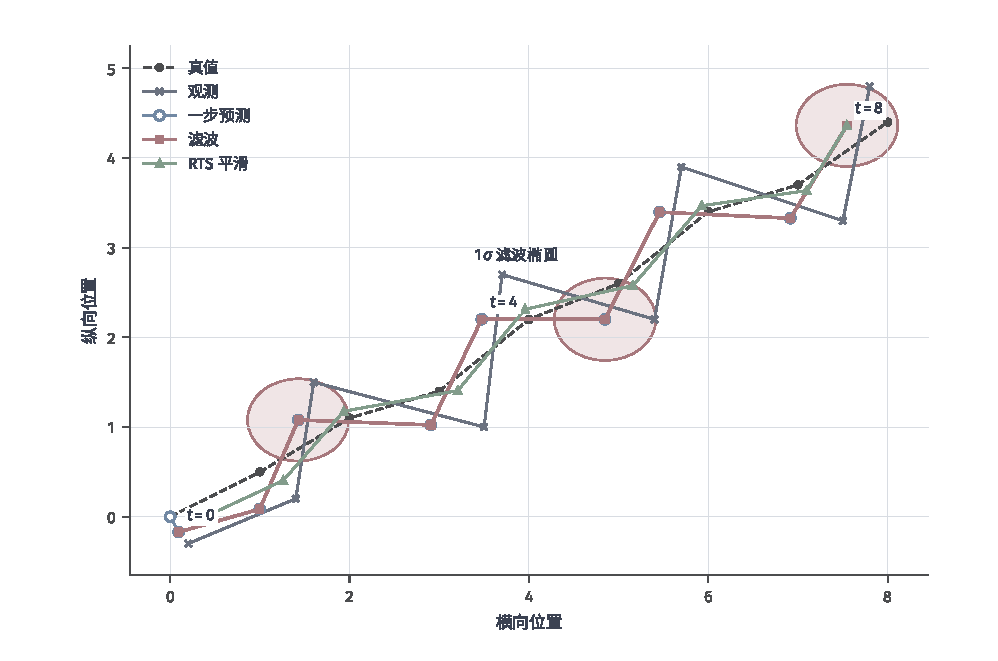
\includegraphics[width=159.059mm]{figures/06-probabilistic-graphical-models/04-models/matplotlib/pgm-dynamic-kalman-trajectory/figure.pdf}
  \caption{人工二维轨迹上的Kalman滤波与RTS平滑。黑色虚线为真值，灰叉为观测，蓝色空心点为观测前预测，红色方点为在线滤波均值，绿色三角为读取全部九次观测的平滑均值。红色半透明椭圆在$t=2,5,8$处显示滤波不确定性，其半轴为各坐标$1$倍标准差；末时刻两类均值重合。图源保存全部参数和坐标，结果对应这组固定的随机游走假设与观测。}
  \label{fig:pgm-dynamic-kalman-trajectory}
\end{figure*}

例~\ref{ex:pgm-dynamic-kalman}第二时刻的更新也可以直接看密度（图~\ref{fig:pgm-dynamic-gaussian}）。观测似然集中在$2$附近，预测密度集中在$0.5$附近，相乘并归一化后，后验均值位于$1.4$。测量与预测共同约束同一状态，使后验方差缩小。

\begin{figure}[htbp]
  \centering
  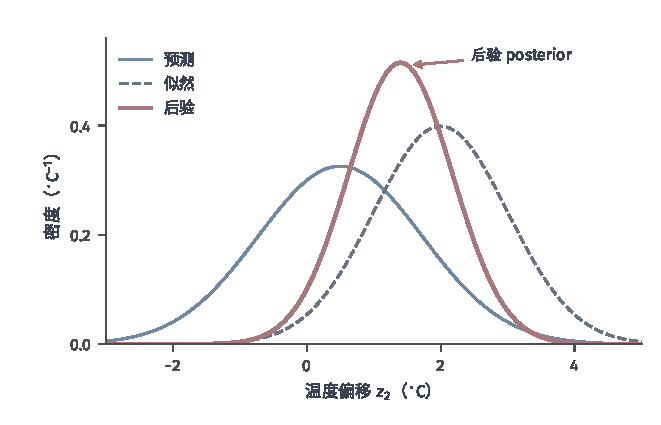
\includegraphics[width=105.412mm]{figures/06-probabilistic-graphical-models/04-models/matplotlib/pgm-dynamic-gaussian/figure.pdf}
  \caption{标量Kalman更新中的预测、似然与后验。蓝色实线表示预测$\mathcal{N}(0.5,1.5)$，灰色虚线表示对状态归一化的似然$\mathcal{N}(2,1)$，红色粗线表示后验$\mathcal{N}(1.4,0.6)$。图例区分三条曲线，红色引线标出后验。横轴为温度偏移，纵轴为密度。这里观测矩阵为$1$，观测似然对状态归一化后恰好形成图示高斯密度。}
  \label{fig:pgm-dynamic-gaussian}
\end{figure}

未知的线性映射和噪声协方差，可以用状态后验统计量来估计。线性高斯EM先计算完全数据对数似然需要的一阶、二阶矩，再拟合转移与观测分布。这与Baum--Welch按软计数学习的结构相同，区别在于连续状态用矩保存期望。当前参数下所需的统计量为
\begin{equation}
  \begin{aligned}
    \overline{\bm{z}}_t&=\bm{m}_{t\mid T},\\
    \bm{M}_t
      &:=\mathbb{E}[\bm{z}_t\bm{z}_t^\top\mid\bm{x}_{1:T}]
        =\bm{P}_{t\mid T}
          +\overline{\bm{z}}_t\overline{\bm{z}}_t^\top,\\
    \bm{M}_{t,t-1}
      &:=\mathbb{E}[\bm{z}_t\bm{z}_{t-1}^\top\mid\bm{x}_{1:T}]\\
      &=\bm{P}_{t,t-1\mid T}
          +\overline{\bm{z}}_t\overline{\bm{z}}_{t-1}^\top.
  \end{aligned}
  \label{eq:pgm-dynamic-em-moments}
\end{equation}
这些期望由同一组旧参数下的滤波和平滑结果给出，在整个M步中保持固定。Ghahramani和Hinton给出了线性系统EM的完全数据似然及相应充分统计量的推导\scite{pgm-dynamic-ghahramani1996}。

M步怎样使用这些矩，可以从残差展开看出。记转移残差$\bm r_t(\bm A)=\bm z_t-\bm A\bm z_{t-1}$，其期望外积为
\begin{equation}
  \begin{aligned}
    \bm{E}_t(\bm{A})
      &:=\mathbb{E}\bigl[
        \bm r_t(\bm A)\bm r_t(\bm A)^\top
        \mid\bm{x}_{1:T}\bigr]\\
      &=\bm{M}_t-\bm{A}\bm{M}_{t,t-1}^{\top}
        -\bm{M}_{t,t-1}\bm{A}^{\top}\\
      &\quad{}+\bm{A}\bm{M}_{t-1}\bm{A}^{\top}.
  \end{aligned}
  \label{eq:pgm-dynamic-transition-residual}
\end{equation}
观测残差的期望外积$\bm{D}_t(\bm{C})$同样展开为
\[
  \begin{aligned}
    \bm{D}_t(\bm{C})
      &=\bm{x}_t\bm{x}_t^\top
        -\bm{C}\overline{\bm{z}}_t\bm{x}_t^\top
        -\bm{x}_t\overline{\bm{z}}_t^\top\bm{C}^\top\\
      &\quad{}+\bm{C}\bm{M}_t\bm{C}^\top.
  \end{aligned}
\]
转移与观测的高斯对数密度包含协方差行列式和加权残差二次型。将二次型写成迹、再取后验期望，EM辅助目标为
\begin{equation}
  \begin{aligned}
    \mathcal Q
      &=-\frac{T-1}{2}\log|\bm Q|
        -\frac12\sum_{t=2}^{T}
          \operatorname{tr}\{\bm Q^{-1}\bm E_t(\bm A)\}\\
      &\quad{}-\frac{T}{2}\log|\bm R|
        -\frac12\sum_{t=1}^{T}
          \operatorname{tr}\{\bm R^{-1}\bm D_t(\bm C)\}\\
      &\quad{}+\text{初始项}+\text{常数}.
  \end{aligned}
  \label{eq:pgm-dynamic-lgssm-q}
\end{equation}
辅助目标把M步分成线性回归和协方差估计。回归使用完整后验二阶矩，因此平滑均值之外的状态不确定性也进入残差与参数更新。

当$T\geq2$、观测完整且相关二阶矩和可逆时，对$\bm A$求导得到回归的正规方程
\[
  \bm A^{(k+1)}\sum_{t=2}^{T}\bm M_{t-1}
    =\sum_{t=2}^{T}\bm M_{t,t-1}.
\]
观测映射满足相同形式的回归方程。先更新两个映射，再用新映射计算期望残差，得到
\begin{equation}
  \begin{aligned}
    \bm A^{(k+1)}
      &=\left(\sum_{t=2}^{T}\bm M_{t,t-1}\right)
        \left(\sum_{t=2}^{T}\bm M_{t-1}\right)^{-1},\\
    \bm C^{(k+1)}
      &=\left(\sum_{t=1}^{T}
        \bm x_t\overline{\bm z}_t^\top\right)
        \left(\sum_{t=1}^{T}\bm M_t\right)^{-1},\\
    \bm Q^{(k+1)}
      &=\frac{1}{T-1}\sum_{t=2}^{T}
        \bm E_t(\bm A^{(k+1)}),\\
    \bm R^{(k+1)}
      &=\frac{1}{T}\sum_{t=1}^{T}
        \bm D_t(\bm C^{(k+1)}).
  \end{aligned}
  \label{eq:pgm-dynamic-lgssm-m-step}
\end{equation}
对$\bm Q^{-1}$或$\bm R^{-1}$求导即可得到协方差更新，例如转移项满足$(T-1)\bm Q=\sum_t\bm E_t$。单条序列的初始参数更新为$\bm m_0^{(k+1)}=\overline{\bm z}_1$、$\bm P_0^{(k+1)}=\bm P_{1\mid T}$。对$n$条独立序列，$\bm m_0^{(k+1)}$取初始平滑均值的平均，$\bm P_0^{(k+1)}$取各初始平滑协方差与初始均值相对总体均值外积之和的平均。转移残差按$\sum_{\ell=1}^{n}(T_\ell-1)$归一化，观测残差按$\sum_{\ell=1}^{n}T_\ell$归一化。初始协方差这样同时保存序列内部的不确定性和各序列起点之间的差异。

将例~\ref{ex:pgm-dynamic-kalman}的平滑结果代入，得到$M_1=0.4+0.8^2=1.04$、$M_2=0.6+1.4^2=2.56$及$M_{2,1}=0.2+1.4\times0.8=1.32$。旧参数$A=C=Q=R=1$下算出的这组矩，给出一次无约束M步：
\[
  \begin{aligned}
    A^{(k+1)}&=1.32/1.04=33/26,\\
    C^{(k+1)}&=(1\times0.8+2\times1.4)/(1.04+2.56)=1,\\
    Q^{(k+1)}&=2.56-1.32^2/1.04=23/26,\\
    R^{(k+1)}&=(1^2+2^2-3.6)/2=0.7.
  \end{aligned}
\]
初始均值与方差分别变为$0.8$和$0.4$。更新得到$A^{(k+1)}>1$，说明无约束极大化可以选择增长的动力学；只有两个观测时，全部系统参数的识别还缺少数据支持。若目标要求稳定动力学，可在$\bm A$的谱半径上施加约束，并求解对应M步。

每轮EM完成滤波、平滑和矩的累计，固定维度时成本随总序列长度线性增长。可以结合似然增量与迭代上限停止，并比较多组初值的观测预测。二阶矩和奇异时，回归可能有多个解；协方差落到退化边界时，需要处理低维支撑。协方差下界、先验、已知噪声结构或固定参数可以约束这些问题，对应目标和更新也随之改变。

连续状态的坐标也有等价表示。对任意可逆矩阵$\bm H$，改用$\widetilde{\bm z}_t=\bm H\bm z_t$，并同时变换$\widetilde{\bm A}=\bm H\bm A\bm H^{-1}$、$\widetilde{\bm C}=\bm C\bm H^{-1}$、$\widetilde{\bm Q}=\bm H\bm Q\bm H^\top$和初始分布，观测分布保持不变。把某个坐标解释成温度或磨损程度，需要测量关系等额外约束。若一个非零方向始终不被$\bm C,\bm C\bm A,\ldots$观测到，数据对该方向的约束还可能不足。因此，后验计算、状态识别和长期误差控制分别依赖相应的模型条件。

单一线性机制适合的响应范围终究有限。下一小节仍保留连续状态，放开线性或高斯条件，考察后验积分怎样近似；由离散模式选择不同连续机制的另一种结构，则在第~\ref{sec:pgm-dynamic-mixed}节单独建立。

\subsection{非线性或非高斯的连续状态建模}
\label{sec:pgm-dynamic-nonlinear-model}

非线性动力学以及偏斜、离群点或离散跳变等噪声特征，可以用更一般的状态空间模型表示。具有加性噪声结构时，写为
\begin{equation}
  \bm z_t=f_t(\bm z_{t-1})+\bm\varepsilon_t,\qquad
  \bm x_t=h_t(\bm z_t)+\bm\eta_t.
  \label{eq:pgm-dynamic-nonlinear}
\end{equation}
直接指定转移和观测分布，还可以表示非加性、非高斯机制。Bayes递推式~\eqref{eq:pgm-dynamic-bayes-filter}依然适用，但单个高斯通常无法精确保存更新后的后验。下列方法分别在局部函数、积分矩或路径后验上近似，由此保留不同的信息。

转移函数、观测函数、噪声分布和初态仍共同构成模型；若它们依赖待估参数，就分别写为$f_{t,\bm\theta}$、$h_{t,\bm\theta}$及相应参数化密度。当前分支只讨论连续状态，离散模式与连续量的组合另见下一节。观测似然目标仍是
\begin{equation}
  \ell_{\mathrm{NL}}(\bm\theta)
    =\sum_n\log\int p_{\bm\theta}(\bm z_1)
      \prod_{t=2}^{T_n}p_{\bm\theta}(\bm z_t\mid\bm z_{t-1})
      \prod_{t=1}^{T_n}p_{\bm\theta}(\bm x_t^{(n)}\mid\bm z_t)
      \,\mathrm d\bm z_{1:T_n}.
  \label{eq:pgm-dynamic-nonlinear-objective}
\end{equation}
困难在于路径积分一般不再有高斯闭式。若采用近似EM，E步近似整段后验的初态、转移及观测统计，M步优化这些期望构成的辅助目标；一般非线性参数化要用数值优化，不能直接沿用线性回归更新。先明确以下工具各自返回什么状态分布，再决定它是否提供学习所需的整段统计。

一旦转移或观测函数非线性，高斯经过它一般不再是高斯，精确闭合被打破。最直接的补救是工程上常用的一阶近似：在当前均值处把非线性函数\emph{泰勒展开}到一阶、用其Jacobian当作线性化矩阵，于是这一步又能套用Kalman公式。它简单廉价，但只有在后验很集中、线性化误差可忽略时才准。在当前估计附近用一阶线性函数近似动力学和观测函数，就可以继续传播高斯均值与协方差。这形成\term{扩展Kalman滤波}（extended Kalman filter, EKF）。对加性高斯噪声，记$\bm F_t$为$f_t$在$\bm m_{t-1\mid t-1}$处的Jacobian，$\bm H_t$为$h_t$在预测均值处的Jacobian，预测计算为
\[
  \begin{aligned}
    \bm m_{t\mid t-1}&\approx f_t(\bm m_{t-1\mid t-1}),\\
    \bm P_{t\mid t-1}
      &\approx\bm F_t\bm P_{t-1\mid t-1}\bm F_t^\top+\bm Q_t,\\
    \bm S_t&\approx\bm H_t\bm P_{t\mid t-1}\bm H_t^\top+\bm R_t.
  \end{aligned}
\]
观测更新以$h_t(\bm m_{t\mid t-1})$为预测读数，以$\bm P_{t\mid t-1}\bm H_t^\top\bm S_t^{-1}$为增益。函数可微、后验集中在线性化有效区域时，局部函数及其矩的近似较为适用。初值偏离、强曲率或分离的后验峰会削弱这种局部表示。

EKF只在一个点上做线性化，强曲率时偏差很大，还要求算导数。无迹变换换一个思路：与其近似函数，不如挑少数几个精心选取的“代表点”（它们恰好匹配输入高斯的均值和协方差），让这些点\emph{原样}通过真正的非线性函数，再用变换后的点加权估计输出的均值和协方差，从而在不求导的情况下捕捉到一部分曲率。也可以让少量代表点直接经过非线性函数，用输出点估计变换后的矩。\term{无迹变换}（unscented transform, UT）选择确定性点来匹配输入均值与协方差，因而省去Jacobian计算。给定$q$维高斯近似$\mathcal N(\bm m,\bm P)$，取$\bm L\bm L^\top=\bm P$、$\kappa>0$，一种$2q+1$点规则为
\[
  \begin{aligned}
    \bm\chi_0&=\bm m,&w_0&=\frac{\kappa}{q+\kappa},\\
    \bm\chi_i&=\bm m+\sqrt{q+\kappa}\bm L_{:,i},
      &w_i&=\frac{1}{2(q+\kappa)},\\
    \bm\chi_{q+i}&=\bm m-\sqrt{q+\kappa}\bm L_{:,i},
      &w_{q+i}&=\frac{1}{2(q+\kappa)},
  \end{aligned}
\]
这里$i=1,\ldots,q$。对称点及其权重恰好恢复输入的$\bm m,\bm P$。经过$f$后，加权均值$\widehat{\bm\mu}=\sum_iw_i f(\bm\chi_i)$和协方差$\sum_iw_i(f(\bm\chi_i)-\widehat{\bm\mu})(f(\bm\chi_i)-\widehat{\bm\mu})^\top$近似输出矩。将这一规则用于预测状态、预测观测和两者的交叉协方差，再按高斯分布条件化，得到\term{无迹Kalman滤波}（unscented Kalman filter, UKF）。

例如$Z\sim\mathcal N(0,1)$经过$f(Z)=Z^2$。在$0$处，函数值和导数均为$0$，EKF给出的均值、方差都是$0$，精确结果则为$1$和$2$。取$q=1,\kappa=2$，代表点$0,\sqrt3,-\sqrt3$对应权重$2/3,1/6,1/6$，输出为$0,3,3$，加权后恰好恢复均值$1$、方差$2$。这个例子展示了代表点怎样捕捉均值附近的曲率。对其他函数，积分矩仍有近似误差；UKF还将条件后验压缩成一个高斯，分离的多个峰因此会丢失。Särkkä和Svensson讨论了EKF、UT及平滑扩展的条件与算法\scite{pgm-dynamic-sarkka2023}。

EKF、UKF都把后验强行压成一个高斯，遇到多峰（状态有几个互斥的可能解释）时会失效。另一类做法不去逐时刻递推某个特定形式，而是直接为\emph{整条状态路径}挑选一个计算得起的近似分布，用第7章的变分思想让它尽量贴近真实后验，从而能保留多峰或跨时刻相关等更丰富的结构。整段状态重建或参数学习还可以直接近似路径后验。\term{变分状态估计}（variational state estimation）选择可计算的路径分布$q_{\bm\phi}(\bm z_{1:T}\mid\bm x_{1:T})$，通过最大化证据下界拟合它（第~\ref{chap:pgm-variational}章）。在线性或局部二次近似下，结构化高斯族可保留相邻时刻的相关性；在下一节的切换系统中，这个思路还可扩展为离散模式链和连续状态链的联合近似。近似族确定了哪些依赖和后验形状能够保存。

对单条序列，其路径变分目标具体为
\begin{equation}
  \begin{aligned}
  \mathcal L(\bm\theta,\bm\phi;\bm x)
    &=\mathbb E_{q_{\bm\phi}(\bm z\mid\bm x)}
        \biggl[\log p_{\bm\theta}(\bm z_1)
        +\sum_{t=2}^{T}\log p_{\bm\theta}(\bm z_t\mid\bm z_{t-1})\\
    &\qquad{}+\sum_{t=1}^{T}\log p_{\bm\theta}(\bm x_t\mid\bm z_t)
        -\log q_{\bm\phi}(\bm z\mid\bm x)\biggr].
  \end{aligned}
  \label{eq:pgm-dynamic-path-elbo}
\end{equation}
共享编码器可以由读数给出近似分布参数，也可以为每条序列直接设置局部变分参数；$\bm\phi$表示相应的待优化量。固定$\bm\theta$、只更新$\bm\phi$是近似状态推断；联合训练则最大化各记录下界之和，交替或联合更新两组参数。梯度中的期望需按近似族解析计算、重参数化或采样估计，并满足相应的可微与可积条件。联合学习时，下界由观测对数似然和近似后验误差共同决定，优化过程中两者都可能变化；模型的预测表现仍需单独评价。

当后验多峰、偏斜、甚至任意形状时，用一个高斯或几个参数都难以刻画，最普适的办法是退回到第8章的蒙特卡洛思想：用一大把带权重的状态\emph{样本（粒子）}来非参数地表示整个后验分布，多个峰可以同时被不同粒子占据，权重则按观测不断更新。分离的后验峰对应不同状态解释，可以用一组样本同时保留。\term{粒子滤波}（particle filtering）以带权状态样本近似滤波分布。设粒子数$n$，第$i$个粒子为$\bm z_{t,i}$，按$q_t(\bm z_t\mid\bm z_{t-1,i},\bm x_t)$提议。在尚未重采样的一步，权重更新为
\[
  w_{t,i}\propto w_{t-1,i}
    \frac{p(\bm x_t\mid\bm z_{t,i})
      p(\bm z_{t,i}\mid\bm z_{t-1,i})}
      {q_t(\bm z_{t,i}\mid\bm z_{t-1,i},\bm x_t)}.
\]
若先按旧权重重采样祖先，祖先选择已计入旧权重，新权重只需当前的重要性比率。序贯重要性更新及带重采样的自举滤波见式~\eqref{eq:pgm-sampling-sis-weight}与算法~\ref{alg:pgm-sampling-bootstrap}。它们用样本和加权和代替难以解析的积分。转移先验提议可约去权重中的转移项；观测集中时，却可能让大量粒子落在低似然区域。每步需要约$n$次转移、似然求值以及重采样，维度与时间跨度影响所需粒子数。固定$n$时，应检查权重集中和样本覆盖。

长期重采样可能使许多粒子共享早期祖先，降低过去路径的多样性。因此，离线平滑和EM还需粒子平滑或其他路径后验方法，计算选择取决于任务需要保留的状态或路径不确定性。



\section{离散模式与连续状态的联合建模}
\label{sec:pgm-dynamic-mixed}

前面要么用离散链（HMM，状态是模式但无法刻画模式内细腻的连续变化），要么用连续状态空间（LGSSM，全程服从同一套线性动态，无法表达“系统在几套截然不同的运行机制之间切换”）。但很多真实过程两者兼有：设备在升温、恒温、冷却等\emph{离散模式}间切换，而在每个模式内部温度又近似服从各自的\emph{线性高斯}动态。把两层结合起来，让离散模式去选择当前用哪一套连续动态方程，就得到切换线性动态系统。有些设备既有升温、恒温等离散运行模式，又有各模式内连续变化的温度。只选择离散或连续一种状态，会把两种不同的信息挤在同一表示里。我们可以让离散模式选择局部连续机制，保留两层不确定性，并组合前面两类模型的计算。

升温、恒温和冷却可能各自近似线性，却使用不同的转移参数。\term{切换线性动态系统}（switching linear dynamical system, SLDS）引入离散模式$S_t\in\{1,\ldots,L\}$，按模式选择连续转移与观测机制。这里$S_t$表示运行模式，与四节点例中传感器失灵变量$S$分别定义。一个常见形式为
\begin{equation}
  \begin{aligned}
    p(s_t\mid s_{t-1})&=\omega_{s_{t-1},s_t},\\
    \bm z_t\mid\bm z_{t-1},s_t
      &\sim\mathcal N(\bm A_{s_t}\bm z_{t-1},\bm Q_{s_t}),\\
    \bm x_t\mid\bm z_t,s_t
      &\sim\mathcal N(\bm C_{s_t}\bm z_t,\bm R_{s_t}),
  \end{aligned}
  \label{eq:pgm-dynamic-switching}
\end{equation}
指定$p(s_1)$与条件高斯初始分布$p(\bm z_1\mid s_1)=\mathcal N(\bm z_1;\bm m_{0,s_1},\bm P_{0,s_1})$后，就能按这些局部机制生成完整序列。图~\ref{fig:pgm-dynamic-switching}显示模式对连续状态与观测的影响。推断时模式也未知，需同时保留可能模式与各模式下的状态不确定性。

\begin{figure}[htbp]
  \centering
  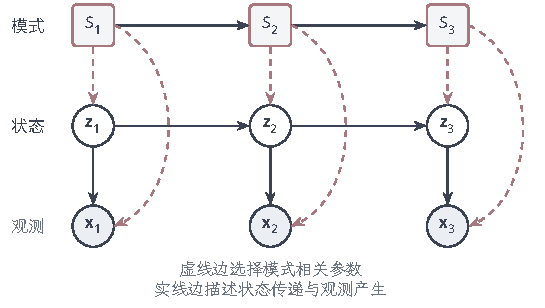
\includegraphics[width=92.276mm]{figures/06-probabilistic-graphical-models/04-models/tikz/pgm-dynamic-switching/figure.pdf}
  \caption{切换系统的三层依赖。方形节点表示离散模式，空心圆表示连续状态，填色圆表示观测。每条完整模式路径对应一组线性高斯递推；到达相同当前模式的不同历史仍可产生不同高斯后验。}
  \label{fig:pgm-dynamic-switching}
\end{figure}

这些局部分布需要组合成同一个联合模型，才能确定哪些模式路径进入训练。完整结构与目标为
\begin{equation}
  \begin{aligned}
    p_{\bm\theta}(s,z,x)
      &=p_{\bm\theta}(s_1)p_{\bm\theta}(\bm z_1\mid s_1)
        \prod_{t=2}^{T}p_{\bm\theta}(s_t\mid s_{t-1})
                           p_{\bm\theta}(\bm z_t\mid\bm z_{t-1},s_t)\\
      &\qquad{}\times\prod_{t=1}^{T}
                           p_{\bm\theta}(\bm x_t\mid\bm z_t,s_t),\\
    \ell_{\mathrm{SLDS}}(\bm\theta)
      &=\sum_n\log\sum_{s_{1:T_n}}\int
                   p_{\bm\theta}(s,z,x^{(n)})\,\mathrm d\bm z_{1:T_n}.
  \end{aligned}
  \label{eq:pgm-dynamic-switching-objective}
\end{equation}
模式概率以及每种模式的映射、噪声与初态都是待估参数。式中的求和保留运行模式的不确定性，积分保留同一模式路径内的连续不确定性。只保留最可能模式再拟合连续量，会改变此处的似然目标。

固定模式历史$s_{1:t}$时，连续状态后验为高斯；换一条历史，均值和协方差一般随之改变。精确滤波把这些历史加在一起，最多形成$L^t$个高斯分量。合并、剪枝或限制每种当前模式的分量数，以近似换取可控成本。EM同时需要模式转移期望计数与各模式的连续二阶矩，E步的混合推断质量因而直接影响学习。

更新所需统计量可以从完全数据分解直接读出。以下期望均在旧参数的整段联合平滑后验下计算，$\sum_{n,t\geq2}$表示汇总每条序列内部的转移。模式转移的更新为
\[
  \omega_{i,j}^{\mathrm{new}}
    =\frac{\sum_{n,t\geq2}p(S_{t-1}=i,S_t=j\mid x^{(n)})}
           {\sum_{n,t\geq2}p(S_{t-1}=i\mid x^{(n)})}.
\]
对当前模式$j$，先累计由$\mathbf1\{S_t=j\}$加权的连续矩和模式占用量：
\[
  \begin{aligned}
    \bm U_j&=\sum_{n,t\geq2}\mathbb E[
       \mathbf1\{S_t=j\}\bm z_{t-1}\bm z_{t-1}^{\top}\mid x^{(n)}],\\
    \bm V_j&=\sum_{n,t\geq2}\mathbb E[
       \mathbf1\{S_t=j\}\bm z_t\bm z_{t-1}^{\top}\mid x^{(n)}],\\
    w_j&=\sum_{n,t\geq2}p(S_t=j\mid x^{(n)}).
  \end{aligned}
\]
于是局部回归与噪声更新为
\begin{equation}
  \begin{aligned}
    \bm A_j^{\mathrm{new}}&=\bm V_j\bm U_j^{-1},\\
    \bm r_{t,j}&=\bm z_t-\bm A_j^{\mathrm{new}}\bm z_{t-1},\\
    \bm Q_j^{\mathrm{new}}
      &=\frac{1}{w_j}\sum_{n,t\geq2}\mathbb E[
       \mathbf1\{S_t=j\}\bm r_{t,j}\bm r_{t,j}^{\top}\mid x^{(n)}].
  \end{aligned}
  \label{eq:pgm-dynamic-switching-update}
\end{equation}
这与线性高斯EM使用相同的回归与残差原理，但每项由当前模式的后验概率加权。观测映射$\bm C_j$的回归分别需要观测与状态的后验交叉矩，以及状态的后验二阶矩：
\[
 \begin{aligned}
  &\sum_{n,t}\bm x_t^{(n)}\mathbb E[
          \mathbf1\{S_t=j\}\bm z_t^{\top}\mid x^{(n)}],\\
  &\sum_{n,t}\mathbb E[
          \mathbf1\{S_t=j\}\bm z_t\bm z_t^{\top}\mid x^{(n)}].
 \end{aligned}
\]
第一项乘第二项的逆矩阵给出$\bm C_j$的更新。$\bm R_j$则对观测残差外积按模式占用量归一化。初态概率由各起点的模式边缘平均；每种模式的初始均值与协方差由起点的加权一二阶矩更新。

这些更新要求相应加权矩可逆、模式占用量非零，且没有改变自由协方差设定的额外约束。训练依次执行混合平滑、累计统计、更新模式概率和连续参数，再检查观测目标或相应近似目标；近似E步不能直接继承精确EM的似然单调保证。只有一个模式时，求和消失并退回LGSSM；一般SLDS的连续状态不能精确压成有限个离散类别，因此通常不能化为有限状态HMM。

在式~\eqref{eq:pgm-dynamic-switching}中，可以只抽样离散模式路径，每个粒子内部按给定模式历史运行精确Kalman递推。这种Rao--Blackwell化利用条件线性高斯结构来减少采样对象（第~\ref{chap:pgm-sampling}章）。

每个粒子还必须携带自己的模式历史条件下的高斯参数；只知道当前模式并不足以选定唯一高斯后验。粒子滤波返回当前状态近似，离线EM还需要整段平滑下的模式计数与相邻连续矩，不能用各时刻滤波均值替代。

\section{状态表示、查询与模型选择}
\label{sec:pgm-dynamic-comparison}

本章模型沿状态可见与否、离散或连续、记忆长度、单链或多链、线性或非线性、是否含离散模式切换等维度变化。下面把它们放回同一套状态空间框架，按要描述的状态、要回答的查询以及对应的推断与学习代价横向比较，作为具体任务选型的依据。对同一条报警序列，模型选择需要同时回答状态表达什么、读取哪些证据以及如何学习机制。先综合各模型之间的结构关系，再讨论这些选择对查询和评价的影响。

\subsection{同一骨架上的模型特例与组合}
\label{sec:pgm-dynamic-model-relations}

比较动态有向模型时，先固定要描述的状态与要回答的查询：状态是否可见、取离散值还是连续值，转移保留多长历史，推断可读取哪些时刻的证据。表~\ref{tab:pgm-dynamic-models}据此并列各类模型的条件和计算。DBN作为共同表示框架适用于各行，具体差别来自状态空间、局部分布和依赖假设。

\begin{table*}[htbp]
  \centering
  \small
  \begin{tabularx}{\linewidth}{@{}p{25mm}p{23mm}p{29mm}p{27mm}X@{}}
    \toprule
    模型 & 状态可见性与空间 & 转移假设 & 常见查询 & 推断与学习 \\
    \midrule
    有限Markov链 & 可见、离散 & 按当前状态给出下一状态分布 & 多步预测、长期分布 & 矩阵递推；可见转移计数 \\
    HMM & 隐藏、离散 & 一阶链，几何停留时间 & 滤波、平滑、整条路径 & 前向--后向、Viterbi；Baum--Welch \\
    高阶HMM与HSMM & 隐藏、离散或分段状态 & 更长历史或显式持续时间 & 路径与片段边界 & 扩充状态或片段动态规划；期望计数 \\
    因子HMM & 多条隐藏离散链 & 先验转移分开，观测耦合 & 联合滤波与平滑 & 联合表可精确但指数增长；变分或采样 \\
    线性高斯模型 & 隐藏、连续 & 线性转移与独立高斯噪声 & 状态分布、预测密度 & Kalman滤波、RTS平滑；二阶矩EM \\
    切换线性系统 & 隐藏、离散与连续混合 & 模式选择线性动态 & 模式与连续状态联合查询 & 高斯混合枚举一般指数增长；混合约简或条件粒子方法 \\
    一般状态空间模型 & 隐藏、连续或混合 & 非线性、非高斯等 & 滤波、平滑及预测风险 & 局部线性化、矩近似、变分或粒子方法 \\
    \bottomrule
  \end{tabularx}
  \caption{动态有向模型的状态、转移与计算。各类模型均需指定初始分布，线性高斯精确递推还需高斯初态。近似方法可按后验形状和查询要求组合选择。}
  \label{tab:pgm-dynamic-models}
\end{table*}

从共同框架看，DBN允许一般切片内与跨片依赖，状态空间分解进一步把历史影响集中到一个状态并令当前观测由它产生。HMM与LGSSM随后分别限制状态空间和局部分布，而高阶、显式时长及因子结构改变状态记忆、片段或组成。SLDS把离散选择与连续机制放在同一联合分布中。这些是结构、特例或组合关系；Kalman、Viterbi和粒子算法则是固定模型后回答不同查询的计算方法。

学习目标也要和结构一起比较。可见链最大化完整状态似然，隐藏状态模型最大化观测边缘似然；计算这类目标时，离散模型需要路径期望计数，线性高斯模型需要后验一二阶及相邻矩，混合模型同时需要两者。路径变分法改为优化显式下界。即使两种模型都调用EM或前向消息，这也不保证它们的观测变量、目标和学习统计相同。

有限状态动态规划和Kalman递推每次都将过去压缩成固定大小的精确消息。前者保存$K$个状态概率，后者保存均值向量和协方差矩阵，因而维度固定时，总成本随时间长度线性增长。接口固定仍可能带来昂贵消息：因子HMM需记录$K^M$种联合配置，切换系统的高斯分量又随模式历史增多。评价成本时，应同时给出序列长度、接口维度和消息表示。

\subsection{推断、学习与评价对应不同问题}
\label{sec:pgm-dynamic-evaluation}

证据可用的时刻决定查询算法。在线控制按当前和过去读数滤波，事后检修则可借助未来证据平滑，两者应分别评价。若损失按逐时刻误判数累计，平滑边缘给出相应最优决策；要求完整路径满足转移限制时，则优化联合解释。连续联合高斯后验的均值也是联合密度众数，混合后验中这两个对象却可能分离，平均值甚至位于分量之间的低密度区域。

误差诊断需要同时检查模型和计算。HMM即使精确推断，也可能因状态过少或持续时间假设偏差而预测失配；EKF还增加了局部线性化误差。比较方法时，固定训练与测试的时间边界，以及一步或多步预测目标，再报告预测对数密度与计算成本；有状态参考值时，可同时评价状态误差和后验不确定性覆盖。按时间保持数据边界，才能评价面向未来的预测；打乱时间点或提前读取未来观测会改变这个任务。

共享参数把多个时刻的数据用于估计同一局部机制，在共享假设适用时减少了待估自由度。运行环境变化后，旧的齐次机制可能失配；已知输入、时变参数或模式切换可表示这种变化，新增机制也需要相应数据来识别。选择模型时，先确定任务所需依赖，再检查状态后验的表示与计算成本，使表达范围、可估计性和推断方法相互匹配。

\section{本章小结}
\label{sec:pgm-dynamic-summary}

动态有向分解把过去对未来的影响集中到时间接口上，使新观测能够逐步并入当前判断。DBN规定依赖模板，Markov性规定给定状态后哪些历史可被压缩，时间齐次与参数共享规定机制的复用方式，平稳性规定过程分布在时间平移下的变化。明确各项条件，才能知道递推中保存的消息代表什么。

有限隐藏状态用前向--后向消息累加路径概率，用Viterbi前驱表恢复最优路径，再由Baum--Welch按后验期望计数学习。线性高斯系统用均值和协方差精确保存状态分布，经Kalman滤波与RTS平滑取得一阶、二阶矩，再拟合局部映射与噪声。这两条路线都先以局部消息完成全局推断，再把后验统计量交给参数学习。

设备的当前报警判断、故障追溯和整段工况解释分别对应滤波、平滑和路径查询。状态增多、持续时间复杂或模式与连续动态混合时，精确消息成本上升，局部高斯、变分和粒子方法在不同位置近似。模型的表达假设决定可描述的演化规律，推断与学习决定怎样从观测取得判断，时间隔离的预测评价则检验它在新数据上的适用性。

\Needspace{8\baselineskip}
\paragraph{扩展阅读}
Bishop的PRML第13章从顺序数据展开HMM与线性动态系统，Murphy的教材进一步讨论滤波、平滑和状态估计。阅读时可沿同一观测序列比较各查询的证据范围，并追踪后验消息怎样变成参数学习所需的统计量\scite{bishop2006,pgm-murphy2012}。

\chapter{概率生成模型}
\label{chap:pgm-generative}

生成模型既用于评价给定观测的概率，也用于生成新观测，这两项任务的计算代价可能相差很大。例如，从噪声到图像的网络可以迅速输出样本，而给定图像的密度可能难以求值；采用条件分解的模型可以精确评价完整观测的似然，生成时却可能需要逐个输出分量。图分解、边缘化和近似推断把这些差异落实为具体计算：先确定查询的概率对象，再找出其中未观测的变量，以及需要执行的求和、积分或变量变换。

本章考察三种构造复杂观测分布的机制：潜变量边缘化、可逆变量变换和人工随机过程。每种机制都需要说明分布为何归一化、训练目标如何联系似然，以及生成样本所需的计算。神经网络分别参数化条件分布、可逆映射或局部转移；这些概率角色决定了模型的表达限制、学习误差和查询成本。

\section{概率生成模型的共同问题}
\label{sec:pgm-generative-common}

设训练样本$\bm{x}_1,\ldots,\bm{x}_n$独立同分布地来自未知分布$p_{\mathrm{data}}$，用参数向量$\bm{\theta}$确定的$p_{\bm{\theta}}$近似数据分布。除特别说明外，观测取值于$\mathbb{R}^{d}$，本章用连续密度描述它们：区域上的概率由密度积分得到，单点密度值可以大于$1$。二值或离散观测则用概率质量函数描述，各个取值的质量直接表示其概率。比较模型似然时，各模型需采用相同的观测表示和测度。

\term{概率生成模型}（probabilistic generative model）为可能出现的观测规定一个分布，并据此生成新观测。对显式密度模型，归一化要求$\int p_{\bm{\theta}}(\bm{x})\,\mathrm{d}\bm{x}=1$。最大似然学习最小化
\begin{equation}
  \label{eq:pgm-generative-nll}
  J(\bm{\theta})
  =-\frac{1}{n}\sum_{i=1}^{n}\log p_{\bm{\theta}}(\bm{x}_i).
\end{equation}
计算该目标需要评价每个观测的对数密度。潜变量模型中的积分可能成为主要障碍；只给出噪声到观测的生成程序时，还需要确认观测密度是否存在，以及如何求值。因此，模型的训练规则、密度评价、采样步骤和潜变量推断各有独立的计算要求。

自回归模型用归一化的一维条件分布按链式法则构成联合分布。给定完整观测后，各条件分布可以直接评价；祖先采样则通常按照分解顺序生成各分量（见第~\ref{sec:pgm-static-directed-autoregressive}节）。以此为基线，下面考察三种计算安排：VAE通过潜变量积分定义观测密度，规范化流用双射的体积变化追踪密度，扩散模型通过多次局部随机转移生成观测。

三种机制使用的概率结构有所不同。VAE采用有向潜变量图；离散扩散采用沿人工噪声索引展开的有向Markov链；规范化流依靠确定性双射和变量变换公式，其计算图记录变换依赖，条件独立性仍需由相应概率模型确定。后文还将介绍概率电路：它通过约束计算图的结构支持精确边缘化和条件查询，补充上述三种机制在查询方面的取舍。

本章用一维目标$X\sim\mathcal{N}(0,5)$贯穿三种机制。独立高斯变量相加、标准高斯缩放和以该分布为起点的前向扩散，分别提供可解析的例子。相同的观测分布使比较集中于潜变量含义、密度计算和随机路径，而复杂数据的表达限制将在各机制中另行讨论。

\section{变分自编码器}
\label{sec:pgm-generative-vae}

\subsection{有向潜变量模型}
\label{sec:pgm-generative-latent-model}

潜变量模型用未观测因素解释观测中共同变化的部分：先抽取潜变量，再按给定潜变量的条件分布生成观测。\term{变分自编码器}（variational autoencoder, VAE）为这一生成模型配备可学习的近似后验。生成网络参数化条件分布，推断网络根据观测给出潜变量的近似分布；两者通过变分目标共同训练\scite{kingma2013}

令$\bm{z}\in\mathbb{R}^{k}$，通常取先验$p(\bm{z})=\mathcal{N}(\bm{0},\bm{I}_k)$，再用神经网络输出条件分布$p_{\bm{\theta}}(\bm{x}\mid\bm{z})$的参数。生成联合分布与观测边缘分布为
\begin{equation}
  \label{eq:pgm-generative-vae-joint}
  \begin{aligned}
    p_{\bm{\theta}}(\bm{x},\bm{z})
      &=p(\bm{z})p_{\bm{\theta}}(\bm{x}\mid\bm{z}),\\
    p_{\bm{\theta}}(\bm{x})
      &=\int p(\bm{z})p_{\bm{\theta}}(\bm{x}\mid\bm{z})
          \,\mathrm{d}\bm{z}.
  \end{aligned}
\end{equation}
先验和每个条件分布归一化时，交换非负积分的次序即可证明观测分布归一化。评价某个观测的似然仍需要计算式中的潜变量积分，其难度取决于条件分布的形式和潜变量维数。

对于连续观测，\term{解码器}（decoder）输出给定潜变量时观测分布的参数。常用的各向同性高斯设定为
\begin{equation}
  \label{eq:pgm-generative-gaussian-decoder}
  p_{\bm{\theta}}(\bm{x}\mid\bm{z})
  =\mathcal{N}\bigl(\bm{x};
    \bm{g}_{\bm{\theta}}(\bm{z}),\tau^2\bm{I}_d\bigr),
  \qquad \tau>0.
\end{equation}
其中$\bm{g}_{\bm{\theta}}:\mathbb{R}^{k}\to\mathbb{R}^{d}$给出条件均值，$\tau^2$为条件噪声方差。一次完整生成先抽取$\bm{z}\sim p$，再抽取独立标准高斯噪声$\bm{\eta}$，得到$\bm{x}=\bm{g}_{\bm{\theta}}(\bm{z})+\tau\bm{\eta}$。实际展示也可能只输出条件均值$\bm{g}_{\bm{\theta}}(\bm{z})$；这会省去观测噪声，与式~\eqref{eq:pgm-generative-gaussian-decoder}规定的随机采样对应不同输出。

线性解码器$\bm{g}_{\bm{\theta}}(\bm{z})=\bm{W}\bm{z}+\bm{b}$与独立高斯噪声共同构成线性高斯模型，其中$\bm{W}\in\mathbb{R}^{d\times k}$。将潜变量变换的协方差与噪声协方差相加，得到观测边缘分布（见第~\ref{sec:pgm-static-directed-linear-gaussian}节）：
\[
  p_{\bm{\theta}}(\bm{x})
  =\mathcal{N}\bigl(\bm{x};
    \bm{b},\bm{W}\bm{W}^{\top}+\tau^2\bm{I}_d\bigr).
\]

潜变量后验可以通过配平方求得。对数联合分布中，先验和观测似然的二次项相加，给出后验精度矩阵$\bm{I}_k+\tau^{-2}\bm{W}^{\top}\bm{W}$；线性项进一步确定后验均值：
\begin{equation}
  \label{eq:pgm-generative-linear-posterior}
  \begin{aligned}
    \bm{\Sigma}
      &=\bigl(\bm{I}_k+\tau^{-2}\bm{W}^{\top}\bm{W}\bigr)^{-1},\\
    \bm{m}(\bm{x})
      &=\tau^{-2}\bm{\Sigma}\bm{W}^{\top}(\bm{x}-\bm{b}),\\
    p_{\bm{\theta}}(\bm{z}\mid\bm{x})
      &=\mathcal{N}\bigl(\bm{z};\bm{m}(\bm{x}),\bm{\Sigma}\bigr).
  \end{aligned}
\end{equation}

非线性解码器可以表达弯曲、非高斯的观测分布。此时，$\lVert\bm{x}-\bm{g}_{\bm{\theta}}(\bm{z})\rVert_2^2$通常不再是潜变量的二次式，前述配平方计算便失去适用条件，边缘密度和后验一般需要近似求解。VAE保留式~\eqref{eq:pgm-generative-vae-joint}的生成定义，用近似后验支持参数学习。

\begin{example}[同一观测分布的潜变量解释]
  \label{ex:pgm-generative-gaussian-latent}
  取$Z\sim\mathcal{N}(0,1)$、$E\sim\mathcal{N}(0,1)$且二者独立，令$X=2Z+E$，于是$X\sim\mathcal{N}(0,5)$。观测$x=2$后，
  \[
    p(z\mid x=2)\propto
    \exp\left[-\frac{1}{2}\{z^2+(2-2z)^2\}\right]
    \propto\exp\left[-\frac{5}{2}(z-0.8)^2\right].
  \]
  后验为$\mathcal{N}(0.8,0.2)$。独立观测噪声使多个潜变量取值都可以解释$x=2$，因此给定观测后仍保留潜变量不确定性。后文的Flow则为完整观测规定唯一逆像。
\end{example}

\subsection{VAE目标与摊销后验}
\label{sec:pgm-generative-vae-objective}

观测边缘积分难以求值时，可以用近似后验构造证据下界。将式~\eqref{eq:pgm-generative-vae-joint}的联合分解代入一般ELBO，得到条件对数似然的期望减去后验与先验的KL散度（见式~\eqref{eq:pgm-variational-elbo}）：
\begin{equation}
  \label{eq:pgm-generative-vae-elbo}
  \begin{aligned}
    \mathcal{L}(\bm{\theta},\bm{\phi};\bm{x})
    ={}&\mathbb{E}_{q_{\bm{\phi}}(\bm{z}\mid\bm{x})}
       [\log p_{\bm{\theta}}(\bm{x}\mid\bm{z})]\\
      &-\operatorname{KL}\bigl(
       q_{\bm{\phi}}(\bm{z}\mid\bm{x})\,\|\,p(\bm{z})\bigr)
      \leq\log p_{\bm{\theta}}(\bm{x}).
  \end{aligned}
\end{equation}

\term{编码器}（encoder）根据观测输出$q_{\bm{\phi}}(\bm{z}\mid\bm{x})$的分布参数。同一组权重$\bm{\phi}$在不同观测之间共享，均值和尺度随输入变化；这构成摊销推断，$\bm{\phi}$对应第~\ref{sec:pgm-variational-amortized}节的$\bm{\omega}$。生成参数$\bm{\theta}$属于观测条件分布。图~\ref{fig:pgm-generative-vae}分别表示两套计算：先验与解码器规定生成联合分布，编码器在训练和观测后推断时提供近似后验。

\begin{figure}[htbp]
  \centering
  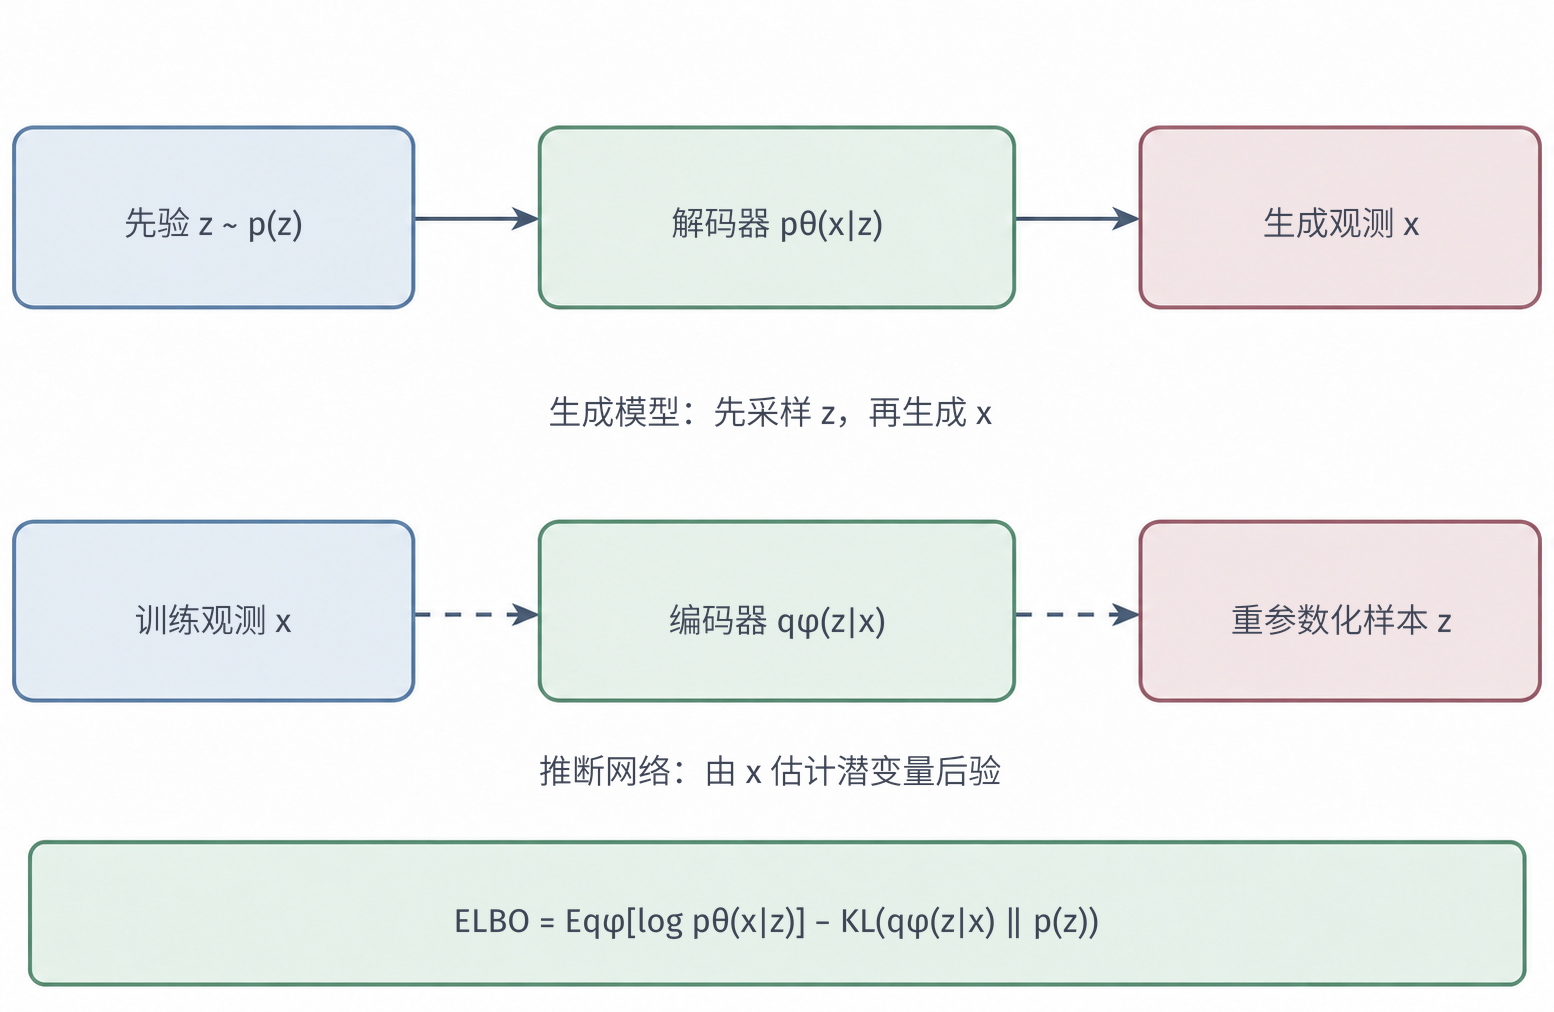
\includegraphics[width=112.000mm]{figures/06-probabilistic-graphical-models/04-models/generated/pgm-generative-vae/figure.png}
  \caption{VAE的生成与近似推断。上行实线表示从先验抽潜变量，再按$p_{\bm\theta}(\bm x\mid\bm z)$抽观测；下行虚线表示由观测构造$q_{\bm\phi}(\bm z\mid\bm x)$。两行分别记录生成分布和推断程序，底部ELBO联系条件似然与近似后验。}
  \label{fig:pgm-generative-vae}
\end{figure}

常用编码器取对角高斯
\[
  q_{\bm{\phi}}(\bm{z}\mid\bm{x})
  =\mathcal{N}\!\left(
    \bm{z};\bm{m}_{\bm{\phi}}(\bm{x}),
    \operatorname{diag}\bigl(\bm{s}_{\bm{\phi}}^2(\bm{x})\bigr)
    \right),
\]
其中每个$s_{\bm{\phi},j}(\bm{x})>0$。网络可以输出对数方差，再经指数变换得到正方差。对标准高斯先验，KL项解析可得：
\begin{equation}
  \label{eq:pgm-generative-diagonal-kl}
  \operatorname{KL}(q_{\bm{\phi}}\,\|\,p)
  =\frac{1}{2}\sum_{j=1}^{k}
     \bigl(m_{\bm{\phi},j}^2+s_{\bm{\phi},j}^2
            -1-\log s_{\bm{\phi},j}^2\bigr).
\end{equation}

式中省略了各分量对观测的依赖。为估计重构期望，抽取独立标准高斯噪声$\bm{\epsilon}$，经$\bm{z}=\bm{m}_{\bm{\phi}}(\bm{x})+\bm{s}_{\bm{\phi}}(\bm{x})\odot\bm{\epsilon}$得到后验样本，其中$\odot$表示逐元素乘法。噪声分布与网络参数无关，梯度可沿均值、尺度和解码器组成的可微路径计算（见第~\ref{chap:pgm-variational}章）。一次编码器前向计算给出当前观测的近似后验参数，省去了逐样本优化变分参数的步骤。

图~\ref{fig:vae-reparameterization-training}表示重参数化后的训练路径：独立噪声经编码器给出的均值与尺度变换为潜变量，重构项的梯度再通过解码器传回编码器。无条件生成采用先验样本进入解码器。

\begin{figure*}[htbp]
  \centering
  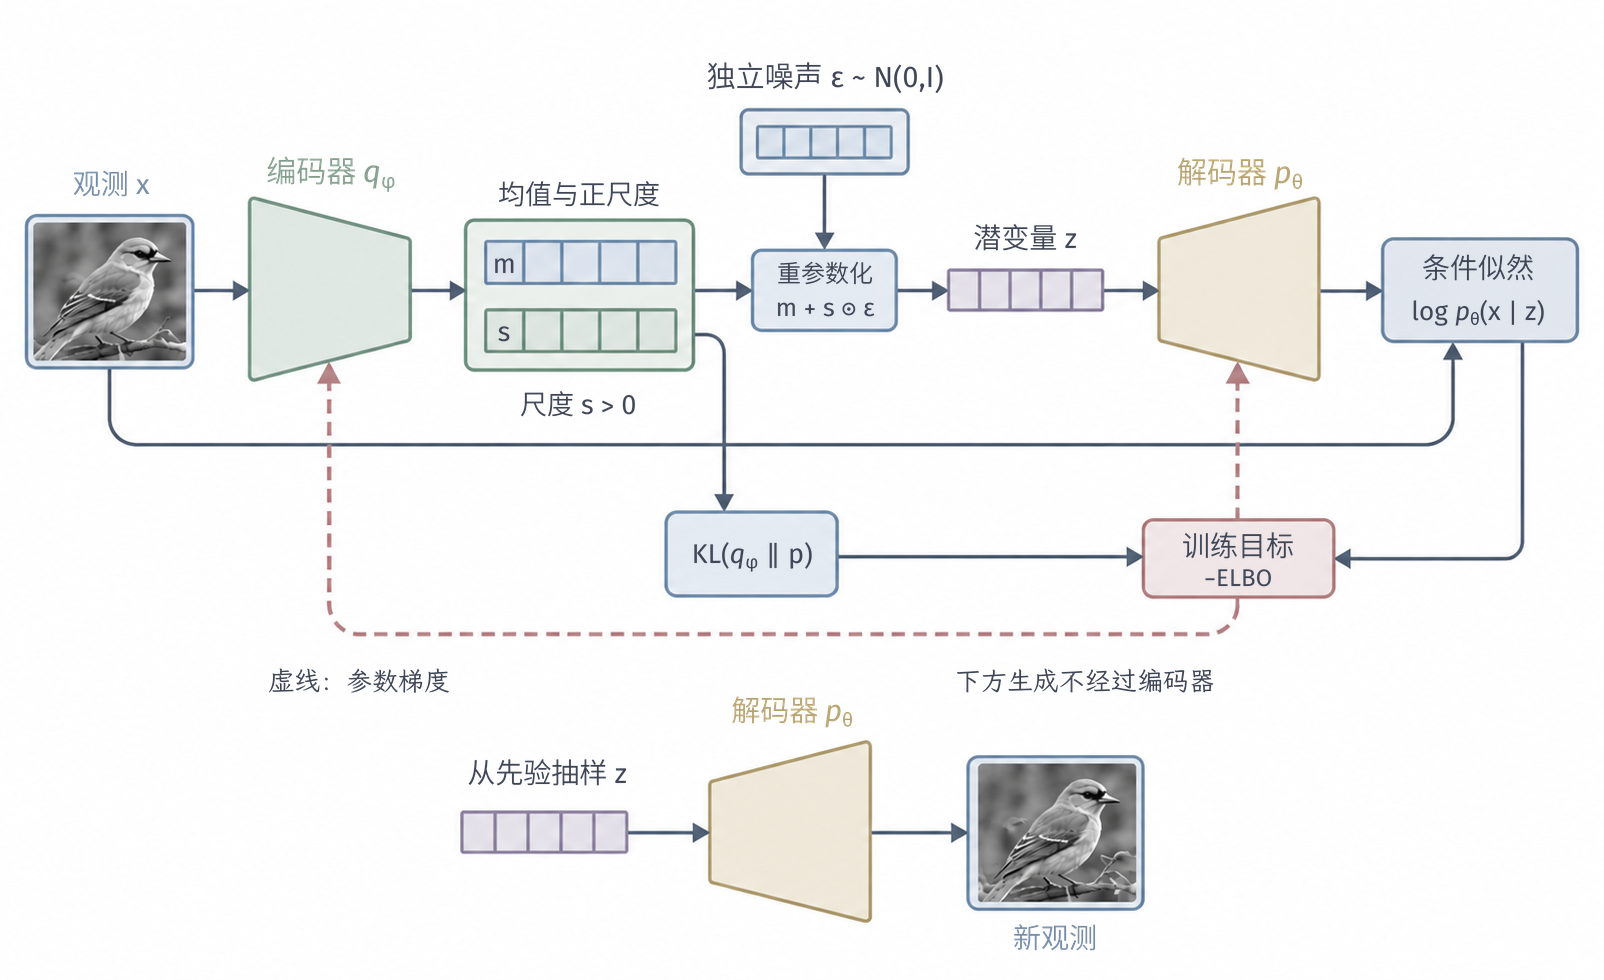
\includegraphics[width=135.805mm]{figures/06-probabilistic-graphical-models/04-models/generated/vae-reparameterization-training/figure.png}
  \caption{对角高斯VAE的重参数化与训练。编码器给出均值$\bm m$和正尺度$\bm s$，独立标准正态噪声经$\bm z=\bm m+\bm s\odot\bm\epsilon$形成潜变量，并进入解码器规定的条件分布。重构对数似然的期望与KL项组成ELBO，图中的负ELBO框表示训练目标。生成阶段从先验抽样，不经过编码器；鸟图为概念插画。}
  \label{fig:vae-reparameterization-training}
\end{figure*}

ELBO中的重构项由观测条件分布确定。对于式~\eqref{eq:pgm-generative-gaussian-decoder}的高斯解码器，负对数似然分解为加权平方误差和方差相关项：
\begin{equation}
  \label{eq:pgm-generative-reconstruction}
  -\log p_{\bm{\theta}}(\bm{x}\mid\bm{z})
  =\frac{\lVert\bm{x}-\bm{g}_{\bm{\theta}}(\bm{z})\rVert_2^2}
          {2\tau^2}
    +\frac{d}{2}\log(2\pi\tau^2).
\end{equation}
固定$\tau$时，最后一项与待学习参数无关。若方差参与学习，对数方差项与平方误差权重共同约束它：增大方差会减轻平方误差的代价，同时提高对数方差代价。删去后一项会改变优化目标。对于二值观测$x_j\in\{0,1\}$，采用给定潜变量后独立的Bernoulli分布，解码器输出参数$\pi_j(\bm{z})$，负对数似然为
\[
  -\sum_{j=1}^{d}
    \bigl[x_j\log\pi_j(\bm{z})
      +(1-x_j)\log(1-\pi_j(\bm{z}))\bigr].
\]

二值交叉熵由此来自Bernoulli观测假设。连续灰度值具有不同的取值空间；对它使用相同表达式时，需说明作为代理损失的含义。离散像素可以采用类别质量函数，也可以将连续条件密度在相应量化区间内积分得到概率质量。

在例~\ref{ex:pgm-generative-gaussian-latent}中，让编码器恰好输出$q(z\mid2)=\mathcal{N}(0.8,0.2)$，可以逐项复核ELBO：
\[
  \begin{aligned}
    \mathbb{E}_{q}(2-2Z)^2&=(2-1.6)^2+4(0.2)=0.96,\\
    \mathbb{E}_{q}\log p(2\mid Z)&=-\tfrac12\log(2\pi)-0.48,\\
    \operatorname{KL}(q\,\|\,p)&=
       \tfrac12\bigl(0.8^2+0.2-1-\log0.2\bigr).
  \end{aligned}
\]
各项相加得到$\mathcal{L}\approx-2.12366$，等于观测对数密度：
\[
  \log\mathcal{N}(2;0,5)
  =-\tfrac12\log(10\pi)-0.4.
\]
将近似后验改为先验时，ELBO降为$-\tfrac12\log(2\pi)-4\approx-4.91894$。两次计算使用相同生成模型，下界差异由近似后验与真实后验的匹配程度引起。

训练时，对小批量观测运行编码器，抽取标准噪声并计算ELBO的随机估计，再更新生成参数和共享编码器参数。停止条件可由计算预算或验证指标确定。设一次编码和解码的代价分别为$C_{\mathrm{enc}}$和$C_{\mathrm{dec}}$；每个观测使用一个潜变量样本时，前向代价约为$O(C_{\mathrm{enc}}+C_{\mathrm{dec}}+k)$，反向传播通常为同阶。增加后验样本可降低部分蒙特卡洛方差，同时增加解码计算。无条件生成只需先验采样和解码；观测后的近似推断只需一次编码器计算。

VAE的误差来自生成分布、近似后验和共享编码器三个层次。\term{模型近似误差}（model approximation error）由候选$p_{\bm{\theta}}$与数据分布的差距产生，需通过调整生成族处理。固定生成参数后，近似后验族的形状限制产生\term{近似族误差}（variational approximation error）。逐个观测的最优变分参数若无法由同一编码器同时表示，还会产生\term{摊销误差}（amortization error）。设$\mathcal{Q}$为候选后验族，$\mathcal{L}_{\mathcal{Q}}^*(\bm{x})=\sup_{q\in\mathcal{Q}}\mathcal{L}(\bm{\theta},q;\bm{x})$为固定模型下该族的最优下界，且$q_{\bm{\phi}}(\cdot\mid\bm{x})\in\mathcal{Q}$。下界差距可分解为
\begin{equation}
  \label{eq:pgm-generative-inference-gaps}
  \begin{aligned}
    \log p_{\bm{\theta}}(\bm{x})
      -\mathcal{L}(\bm{\theta},\bm{\phi};\bm{x})
    ={}&\bigl[\log p_{\bm{\theta}}(\bm{x})
             -\mathcal{L}_{\mathcal{Q}}^*(\bm{x})\bigr]\\
       &+\bigl[\mathcal{L}_{\mathcal{Q}}^*(\bm{x})
             -\mathcal{L}(\bm{\theta},\bm{\phi};\bm{x})\bigr].
  \end{aligned}
\end{equation}

第一项为近似族误差，第二项为当前编码器相对于逐观测最优解的差距，两项均非负。第二项还包含编码器优化不足；进一步比较最优共享编码器，可以区分摊销限制与优化误差（见式~\eqref{eq:pgm-variational-amortization-gap}）。增加生成族容量、扩大后验族和改进编码器优化，分别针对这些不同来源的误差。

\subsection{生成能力与失效模式}
\label{sec:pgm-generative-vae-failure}

潜变量维度决定生成模型可以用多少自由度解释观测变化。即使$k<d$，式~\eqref{eq:pgm-generative-gaussian-decoder}中正方差噪声仍覆盖全部观测维度，使模型具有$d$维密度。去掉噪声后，光滑低维解码器的输出通常集中于低维集合。增大潜变量维度可减轻表示瓶颈，同时增加学习和推断的自由度；这些维度能否承载有效信息，还取决于训练目标与解码器对潜变量的利用。

给定潜变量后若仍存在多种不同观测，固定方差的单一高斯条件似然通过平方误差拟合它们的均值。在有限二阶矩条件下，逐坐标的总体最优预测为$\mathbb E[\bm X\mid\bm z]$（参见\BookTheoremRef{thm:probability-conditional-mean-l2-projection}{卷2《数学准备：概率、因果与决策》第1章“随机变量”第1.2.2.1节“条件信息下的均值关系”}）。例如，边缘等概率出现在左右两处时，均值图像会在两处留下较淡的边缘，这提供了模糊重构的一种解释。表达力更强的条件似然可以分别描述这些结果；在简单高斯均值上增加独立噪声，主要改变随机波动，恢复结构仍需相应条件分布。

编码器还可能几乎不携带观测信息。本节将近似后验接近先验的现象称为\term{后验坍塌}（posterior collapse），即$q_{\bm{\phi}}(\bm{z}\mid\bm{x})\approx p(\bm{z})$；部分坐标也可以单独出现这种现象。该定义针对近似后验，真实后验需由生成模型另行判断。以例~\ref{ex:pgm-generative-gaussian-latent}为例，编码器总输出先验时，生成模型在$x=2$处的真实后验仍为$\mathcal{N}(0.8,0.2)$，两者的差异表现为推断误差。

若解码器忽略全部潜变量，即$p_{\bm{\theta}}(\bm{x}\mid\bm{z})=p_{\bm{\theta}}(\bm{x})$，真实后验便等于先验。固定这一生成模型时，近似后验取先验即可使ELBO达到最大。表达力强的解码器可能在利用潜变量之前就充分拟合数据，此时利用潜变量所得的重构收益未必补偿KL代价，训练也可能停留在这一状态。编码器KL接近零因而提供了坍塌线索；判断真实潜变量依赖还需考察解码分布。解码器本身的生成质量则是另一项评价。

编码器在训练数据上产生的潜变量分布，可能与无条件生成采用的先验分布不同。定义\term{聚合后验}（aggregated posterior）
\begin{equation}
  \label{eq:pgm-generative-aggregated-posterior}
  q_{\mathrm{agg}}(\bm{z})
  =\mathbb{E}_{\bm{X}\sim p_{\mathrm{data}}}
       [q_{\bm{\phi}}(\bm{z}\mid\bm{X})],
\end{equation}
即把不同观测的编码分布按数据频率混合。假设相关KL有限，在$\log(q_{\bm{\phi}}/p)$中加减$\log q_{\mathrm{agg}}$，可得
\begin{equation}
  \label{eq:pgm-generative-kl-information}
  \mathbb{E}_{p_{\mathrm{data}}}
    \operatorname{KL}(q_{\bm{\phi}}(\bm{z}\mid\bm{X})\,\|\,p(\bm{z}))
  =I_q(\bm{X};\bm{Z})+
    \operatorname{KL}(q_{\mathrm{agg}}\,\|\,p).
\end{equation}
其中$I_q$是联合分布$p_{\mathrm{data}}(\bm{x})q_{\bm{\phi}}(\bm{z}\mid\bm{x})$下的互信息。逐样本KL同时约束编码中的数据信息和聚合后验与先验的匹配。有限训练后，先验仍可能在编码器很少访问的区域保留明显质量；无条件生成进入这些区域时，解码器的表现会受到训练支持不足的影响。

不同修正分别改变训练路径、生成结构或推断族。将KL系数从小值逐渐提高到$1$，可以调整训练中重构与先验匹配的相对作用；最终保持$\lambda\ne1$时，$\mathbb{E}_q\log p_{\bm{\theta}}(\bm{x}\mid\bm{z})-\lambda \operatorname{KL}(q\,\|\,p)$则成为不同于原ELBO的目标。$\lambda\geq1$时该目标仍不大于原ELBO，$\lambda<1$时缺少相同的下界保证。限制解码器绕过潜变量的信息通路会改变模型结构，扩大后验族主要减小推断差距，学习可评价密度的先验会改变生成模型和KL的比较对象。修正是否改善潜变量利用，需结合这些对象及实际优化结果判断。

给定标签或其他条件$\bm{c}$时，\term{条件VAE}（conditional VAE）使用条件先验与条件解码分布$p_{\bm{\theta}}(\bm{z}\mid\bm{c})p_{\bm{\theta}}(\bm{x}\mid\bm{z},\bm{c})$，并用$q_{\bm{\phi}}(\bm{z}\mid\bm{x},\bm{c})$近似后验。潜变量可用于表示已知条件之外的剩余变化。

\term{层次VAE}（hierarchical VAE）通过多层随机潜变量表示依赖，例如$p(\bm{z}_2)p_{\bm{\theta}}(\bm{z}_1\mid\bm{z}_2)p_{\bm{\theta}}(\bm{x}\mid\bm{z}_1)$。每一层都规定条件分布，因此同时增加生成模型的随机依赖和后验耦合；确定性解码网络的层数则属于条件分布内部的参数化。

\section{基于可逆变换的密度模型}
\label{sec:pgm-generative-flows}

\subsection{变量变换与精确密度}
\label{sec:pgm-generative-change-of-variables}

多个潜变量及观测噪声可以产生同一观测，因此VAE通过积分评价观测密度。另一种安排是让完整观测与基础变量一一对应，用变换的体积因子计算密度。\term{规范化流}（normalizing flow, Flow，也译为归一化流）将可评价密度的基础分布经一串可逆变换推送到观测空间，并逐层追踪密度变化\scite{pgm-generative-papamakarios2021}

设$\bm Z\sim p_0$，$\bm X=f_{\bm\theta}(\bm Z)$，基础变量与观测均为$d$维。若变换是开集间的连续可微双射，其逆连续可微且Jacobian行列式非零，变量变换公式给出观测密度：
\begin{equation}
  \label{eq:pgm-generative-flow-density}
  \begin{aligned}
    p_{\bm{\theta}}(\bm{x})
      &=p_0(f_{\bm{\theta}}^{-1}(\bm{x}))
         \left|\det\bm{J}_{f_{\bm{\theta}}^{-1}}(\bm{x})\right|,\\
    \log p_{\bm{\theta}}(\bm{x})
      &=\log p_0(\bm{z})-
         \log\left|\det\bm{J}_{f_{\bm{\theta}}}(\bm{z})\right|.
  \end{aligned}
\end{equation}
其中$\bm z=f_{\bm\theta}^{-1}(\bm x)$为观测的逆像，$\bm J_f$为变换的Jacobian矩阵。行列式修正局部体积变化，保留相应区域上的概率质量，归一化由基础分布和变量变换共同保证（参见\BookSectionRef{sec:analysis-coordinate-change-integral-applications}{卷1《数学准备：分析、几何与计算》第3章“测度与分析”第3.4.3.2节“基于坐标换元的积分计算”}和\BookSectionRef{sec:rv-pushforward}{卷2《数学准备：概率、因果与决策》第1章“随机变量”第1.3.1.1节“随机变量的分布变换”}）。采用分段光滑网络时，还需验证变量变换的适用条件；几乎处处可微与双射本身尚不足以保证该密度关系。

若$f=f_K\circ\cdots\circ f_1$，令$\bm{h}_0=\bm{z}$、$\bm{h}_{\ell}=f_{\ell}(\bm{h}_{\ell-1})$、$\bm{h}_K=\bm{x}$，链式法则给出
\begin{equation}
  \label{eq:pgm-generative-flow-composition}
  \log p_{\bm{\theta}}(\bm{x})
  =\log p_0(\bm{h}_0)
   -\sum_{\ell=1}^{K}
      \log|\det\bm{J}_{f_{\ell}}(\bm{h}_{\ell-1})|.
\end{equation}
训练时，从观测沿逆变换恢复基础变量，累积各层对数行列式，便可对式~\eqref{eq:pgm-generative-nll}求梯度。生成时，从基础分布抽样后依次执行正向变换。该训练直接评价模型密度，成本主要取决于逆变换和体积因子的计算：一般稠密$d\times d$矩阵的常规行列式计算需要$O(d^3)$运算，形成完整Jacobian也可能代价较高。因此，网络结构需同时提供可行的逆变换与行列式算法。

\begin{example}[用缩放得到相同的一维密度]
  \label{ex:pgm-generative-gaussian-flow}
  取$Z\sim\mathcal{N}(0,1)$，令$X=\sqrt{5}Z$，同样得到$\mathcal{N}(0,5)$。给定$x=2$，唯一逆像是$z=2/\sqrt5$，因此
  \[
    \log p(2)=-\tfrac12\log(2\pi)
              -\tfrac12(2/\sqrt5)^2-\log\sqrt5
             \approx-2.12366.
  \]
  该观测密度与VAE例子相同，潜变量关系却不同：这里的完整观测唯一确定基础变量，VAE中则保留$\mathcal{N}(0.8,0.2)$的后验不确定性。观测分布相同而潜变量解释不同，表明仅凭观测似然无法识别生成机制。
\end{example}

标准Flow的基础空间与观测空间同维，变量变换中的Jacobian因而是方阵。坐标重排、分块输出和保留旁路变量可以改变张量形状，同时保留总自由度。丢弃坐标时需对它们边缘化；加入随机变量时则需规定扩展空间上的联合密度。

连续Flow用于离散观测时，需要将密度转换为量化区间的概率质量。以单位宽度量化为例，量化值$\bm{y}$的质量为$p(\bm{y})=\int_{[0,1)^d}p_{\mathrm{cont}}(\bm{y}+\bm{u})\,\mathrm{d}\bm{u}$。取$\bm{U}$在单位立方体上均匀分布，Jensen不等式使均匀去量化目标$\mathbb{E}_{\bm{U}}\log p_{\mathrm{cont}}(\bm{y}+\bm{U})$成为该对数质量的下界。若预处理还改变观测尺度，相应Jacobian也参与密度换算。

\subsection{可逆网络结构}
\label{sec:pgm-generative-invertible-networks}

\term{仿射耦合层}（affine coupling layer）通过保留部分坐标，使逆变换和Jacobian行列式都能直接计算。将全部坐标分为两个非空、不相交的块$A,B$，用保留的$A$块决定$B$块的缩放与平移：
\begin{equation}
  \label{eq:pgm-generative-coupling}
  \begin{aligned}
    \bm{x}_A&=\bm{z}_A,\\
    \bm{x}_B&=\bm{z}_B\odot
       \exp\bigl(\bm{a}_{\bm{\theta}}(\bm{z}_A)\bigr)
          +\bm{b}_{\bm{\theta}}(\bm{z}_A).
  \end{aligned}
\end{equation}
逐元素指数保证缩放因子为正。给定输出，先由保留块恢复$\bm{z}_A=\bm{x}_A$，再计算$\bm{z}_B=(\bm{x}_B-\bm{b}_{\bm{\theta}}(\bm{x}_A))\odot\exp(-\bm{a}_{\bm{\theta}}(\bm{x}_A))$。子网络只负责从已知保留块计算参数，其自身可采用一般的非可逆网络。Real NVP用这类耦合变换构造密度模型\scite{pgm-generative-dinh2017}

按$A,B$的顺序排列坐标，Jacobian为
\begin{equation}
  \label{eq:pgm-generative-coupling-jacobian}
  \begin{aligned}
    \bm{J}_{f}
      &=
        \begin{pmatrix}
          \bm{I}&\bm{0}\\
          *&\operatorname{diag}(\exp\bm{a}_{\bm{\theta}}(\bm{z}_A))
        \end{pmatrix},\\
    \log|\det\bm{J}_{f}|
      &=\sum_{j=1}^{|B|}a_{\bm{\theta},j}(\bm{z}_A).
  \end{aligned}
\end{equation}
星号块记录子网络引入的交叉导数；三角结构使行列式只取决于对角缩放项。图~\ref{fig:pgm-generative-coupling}对应这一计算依赖。单层保留$A$块，会限制可表达的变换；多层间交换分块或加入可逆混合后，各坐标可以逐步相互影响。设单层子网络代价为$C$，行列式计算额外需要$O(d)$运算，$K$层正向或逆向计算的总代价约为$O(K(C+d))$。

\begin{figure}[htbp]
  \centering
  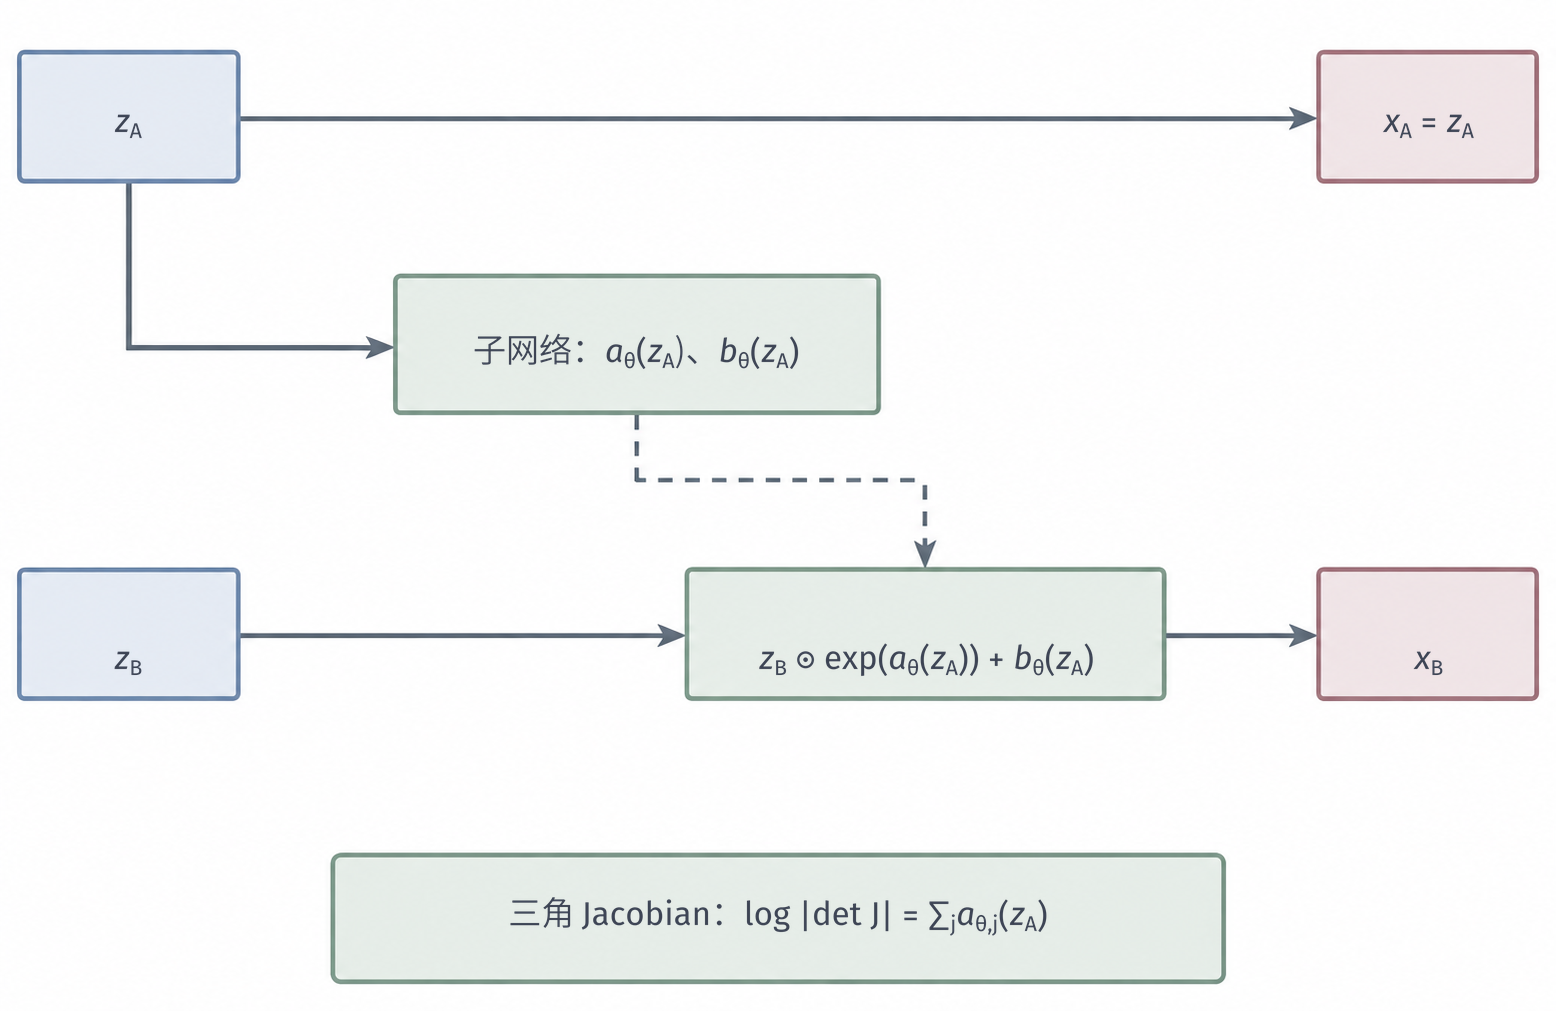
\includegraphics[width=112.000mm]{figures/06-probabilistic-graphical-models/04-models/generated/pgm-generative-coupling/figure.png}
  \caption{仿射耦合层的计算依赖。保留块$\bm z_A$经粗线进入子网络，确定$B$块仿射变换的缩放与平移。Jacobian的下三角结构使对数行列式等于缩放对数之和；逆向计算先恢复$\bm z_A$，再撤销$B$块的平移和缩放。}
  \label{fig:pgm-generative-coupling}
\end{figure}

例如，二维变换$x_1=z_1$、$x_2=2z_2+z_1^2$在$\bm{z}=(1,-1)$处输出$\bm{x}=(1,-1)$，逆变换恢复$z_2=(x_2-x_1^2)/2=-1$。Jacobian为$\left(\begin{smallmatrix}1&0\\2z_1&2\end{smallmatrix}\right)$，行列式恒为$2$。基础分布取二维标准高斯时，该观测的对数密度为$-\log(2\pi)-1-\log2$。非线性项位于Jacobian的非对角块，因此可以改变坐标依赖，同时保留简单的体积因子。

\term{自回归流}（autoregressive flow）通过坐标顺序构造三角Jacobian，用前面坐标计算当前可逆变换的参数。与直接参数化条件分布的自回归模型相比，这里需要同时考察采样方向和密度评价方向的代价（见第~\ref{chap:pgm-static-directed}章）。\term{掩码自回归流}（masked autoregressive flow, MAF）的一种形式为
\[
  x_j=\mu_j(\bm{x}_{<j})+
       \exp(a_j(\bm{x}_{<j}))z_j,\qquad j=1,\ldots,d,
\]
其中$\bm{x}_{<j}=(x_1,\ldots,x_{j-1})$。评价给定$\bm{x}$时，所有条件输入已知，掩码网络可并行给出各$\mu_j,a_j$，从而恢复$\bm{z}$并求出三角Jacobian的行列式；生成时$\bm{x}_{<j}$尚未齐备，必须顺序恢复坐标。

\term{逆自回归流}（inverse autoregressive flow, IAF）将参数输入改为$\mu_j(\bm{z}_{<j})$和$a_j(\bm{z}_{<j})$。全部基础噪声已知时，输出及对应样本密度可并行计算；给定外部观测后，逆变换则需要逐坐标恢复基础变量。因此，IAF适合生成并评价自身样本，MAF适合评价指定观测的密度，二者的顺序代价分别位于不同方向\scite{pgm-generative-papamakarios2017}

连续变换用速度场代替有限层映射。\term{连续规范化流}（continuous normalizing flow, CNF）以常微分方程
\[
  \frac{\mathrm{d}\bm{h}_u}{\mathrm{d}u}
    =\bm{v}_{\bm{\theta}}(\bm{h}_u,u),
  \qquad 0\leq u\leq1,
\]
定义基础变量到观测的映射，起点为$\bm{h}_0=\bm{z}$，终点为$\bm{h}_1=\bm{x}$，$u$表示变换进度。可逆流的一种充分正则设定是：速度场对空间连续可微，满足保证初值问题解唯一性的Lipschitz条件，且解在整个区间正反两向都存在。解的唯一性使不同轨迹在同一进度处保持分离，从而建立一一对应的变换。

记$\rho_u$为$\bm{h}_u$的密度。小步映射的Jacobian为$\bm{I}+\Delta u\,\bm{J}_{\bm{v}}+o(\Delta u)$，结合$\log\det(\bm{I}+\Delta u\,\bm{A})=\Delta u\,\operatorname{tr}\bm{A}+o(\Delta u)$，可从式~\eqref{eq:pgm-generative-flow-density}得到\term{瞬时变量变换公式}（instantaneous change of variables）：
\begin{equation}
  \label{eq:pgm-generative-instantaneous-change}
  \begin{aligned}
    \frac{\mathrm{d}}{\mathrm{d}u}
         \log\rho_u(\bm{h}_u)
       &=-\nabla_{\bm{h}}\!\cdot
          \bm{v}_{\bm{\theta}}(\bm{h}_u,u),\\
    \log p_{\bm{\theta}}(\bm{x})
       &=\log p_0(\bm{z})
         -\int_0^1\nabla_{\bm{h}}\!\cdot
           \bm{v}_{\bm{\theta}}(\bm{h}_u,u)\,\mathrm{d}u.
  \end{aligned}
\end{equation}
散度$\nabla\cdot\bm{v}=\sum_j\partial v_j/\partial h_j$为Jacobian的迹，表示局部体积膨胀率。积分该膨胀率即可追踪密度，因此CNF允许一般的速度场结构，代价转为沿轨迹反复评价速度场与散度。

高维迹计算可以采用随机估计。若随机向量满足$\mathbb{E}\bm{r}=\bm{0}$和$\mathbb{E}\bm{r}\bm{r}^{\top}=\bm{I}$，便有$\operatorname{tr}\bm{A}=\mathbb{E}_{\bm{r}}[\bm{r}^{\top}\bm{A}\bm{r}]$。自动微分通过向量与Jacobian的乘积计算单次估计，FFJORD将这一方法用于连续流\scite{pgm-generative-grathwohl2018}

该恒等式保证固定矩阵下的迹估计无偏，有限样本仍有蒙特卡洛波动。程序还需近似求解状态轨迹和散度积分，因此连续流返回的似然通常同时包含随机估计误差与数值积分误差。正向和逆向计算都依赖求解器，其成本由函数评价次数和速度场的数值性质决定。

\subsection{生成模型与变分后验}
\label{sec:pgm-generative-flow-roles}

规范化流可用于观测分布，也可用于近似后验。作为独立生成模型，它将基础变量变为观测，并由式~\eqref{eq:pgm-generative-flow-density}计算观测密度。用于VAE后验时，它在固定观测下变换简单潜变量分布，构造更灵活的$q_{\bm{\phi}}(\bm{z}\mid\bm{x})$；调整对象是推断族，生成联合分布可以保持原样\scite{pgm-overview-rezende2015}

具体地，从简单条件分布抽取$\bm{u}\sim q_0(\bm{u}\mid\bm{x})$，经$\bm{z}=f_{\bm{\phi}}(\bm{u};\bm{x})$得到后验样本。固定观测后，变换关于基础潜变量满足变量变换条件，后验样本密度便为
\begin{equation}
  \label{eq:pgm-generative-flow-posterior}
  \log q_{\bm{\phi}}(\bm{z}\mid\bm{x})
  =\log q_0(\bm{u}\mid\bm{x})
    -\log\left|
       \det\frac{\partial f_{\bm{\phi}}(\bm{u};\bm{x})}
                     {\partial\bm{u}^{\top}}
      \right|.
\end{equation}
将该密度代入$\mathbb{E}_{q_{\bm{\phi}}}[\log p_{\bm{\theta}}(\bm{x},\bm{z})-\log q_{\bm{\phi}}(\bm{z}\mid\bm{x})]$即可构造训练目标。变换后KL通常需要蒙特卡洛估计，所需联合密度和后验样本密度仍可评价。训练评价的正是本次生成的后验样本，因此可以利用IAF在这一方向上的并行计算。

扩大后验族可以收紧VAE下界，观测边缘密度仍由生成联合分布的积分定义。独立Flow则采用唯一编码$\bm{z}=f^{-1}(\bm{x})$，给定完整观测后的基础变量条件分布为点质量，两者的后验对象因此不同。

标准光滑双射也有表达限制。例如，全空间上正密度的基础分布经过处处非奇异的满射变换后，观测密度仍处处为正。这样的流可以将两个高密度区域之间的概率压低，却无法精确表示仅在两个分离区域具有支撑的密度。实现极小连接概率可能需要极端缩放，进而恶化逆变换和密度计算的数值条件。

\section{扩散与分数生成模型}
\label{sec:pgm-generative-diffusion}

\subsection{前向扰动与逆向生成}
\label{sec:pgm-generative-forward-reverse}

\term{扩散模型}（diffusion model）用逐步扰动把数据分布与简单噪声分布连接起来，并学习从噪声到数据的局部转移。训练观测提供前向加噪状态，生成则沿相反顺序执行学得的转移。下文的$\bm{x}_t$表示某一噪声尺度下的状态，索引$t$由模型人为构造；真实序列的时间索引另由动态模型描述（见第~\ref{chap:pgm-dynamic}章）。

\term{去噪扩散概率模型}（denoising diffusion probabilistic model, DDPM）的一种标准前向过程固定噪声日程$0<\beta_t<1$，$t=1,\ldots,T$，并定义
\begin{equation}
  \label{eq:pgm-generative-forward-chain}
  \begin{aligned}
    q(\bm{x}_{1:T}\mid\bm{x}_0)
      &=\prod_{t=1}^{T}q(\bm{x}_t\mid\bm{x}_{t-1}),\\
    q(\bm{x}_t\mid\bm{x}_{t-1})
      &=\mathcal{N}(\bm{x}_t;
          \sqrt{\alpha_t}\bm{x}_{t-1},\beta_t\bm{I}_d),\\
    \alpha_t&=1-\beta_t,\qquad
    \bar{\alpha}_t=\prod_{s=1}^{t}\alpha_s,\qquad
    \bar{\alpha}_0=1.
  \end{aligned}
\end{equation}
每一步缩小信号并加入独立高斯噪声。条件均值逐步乘以信号衰减系数，条件噪声方差则满足递推$\alpha_t(1-\bar{\alpha}_{t-1})+\beta_t=1-\bar{\alpha}_t$。因此，给定原观测的任意一步分布为
\begin{equation}
  \label{eq:pgm-generative-forward-marginal}
  \begin{aligned}
    q(\bm{x}_t\mid\bm{x}_0)
      &=\mathcal{N}(\bm{x}_t;
          \sqrt{\bar{\alpha}_t}\bm{x}_0,
          (1-\bar{\alpha}_t)\bm{I}_d),\\
    \bm{x}_t&=\sqrt{\bar{\alpha}_t}\bm{x}_0+
              \sqrt{1-\bar{\alpha}_t}\bm{\epsilon},
    \quad \bm{\epsilon}\sim\mathcal{N}(\bm{0},\bm{I}_d).
  \end{aligned}
\end{equation}
训练时可从该条件分布直接抽取任意噪声步，省去之前的逐步扰动计算。式中的标准高斯变量代表当前一步的合成噪声；完整前向路径的跨步依赖仍由式~\eqref{eq:pgm-generative-forward-chain}的逐步独立扰动决定。上述构造及后续目标采用DDPM的固定日程设定\scite{pgm-generative-ho2020}

有限步下，正的$\bar{\alpha}_T$使终点通常仍保留一部分数据结构。生成模型以标准高斯$p(\bm{x}_T)=\mathcal{N}(\bm{0},\bm{I}_d)$作为终端先验，日程需要使前向终点充分接近它。给定原观测时，两者的差距可以通过高斯KL直接计算：
\begin{equation}
  \label{eq:pgm-generative-terminal-kl}
  \begin{aligned}
    &\operatorname{KL}\bigl(
        q(\bm{x}_T\mid\bm{x}_0)\,\|\,p(\bm{x}_T)\bigr)\\
    &\quad=\frac12\left[
       \bar{\alpha}_T\lVert\bm{x}_0\rVert_2^2
       -d\bar{\alpha}_T-d\log(1-\bar{\alpha}_T)
      \right].
  \end{aligned}
\end{equation}
数据二阶矩有限且$\bar{\alpha}_T\to0$时，该条件KL的数据平均趋于零。KL的凸性又使这一平均量控制前向终点边缘$q_T$与先验的KL。有限步下，匹配程度取决于累计信号衰减、数据尺度和观测维度，可用该表达式评价日程选择。

在贯穿例子$X_0\sim\mathcal{N}(0,5)$中，前向边缘可以直接算出：
\begin{equation}
  \label{eq:pgm-generative-gaussian-diffusion}
  q_t(x)=\mathcal{N}(x;0,1+4\bar{\alpha}_t).
\end{equation}
取$\bar{\alpha}_T=0.25$时，终点边缘为$\mathcal{N}(0,2)$，与标准高斯的KL为$\tfrac12(2-1-\log2)\approx0.15343$。取$\bar{\alpha}_T=0.01$时，方差降至$1.04$，KL约为$0.000390$。这里评价的是终点边缘的差距；式~\eqref{eq:pgm-generative-terminal-kl}评价给定原观测的条件差距，其数据平均通常更大。

逆向生成从终端先验抽样，再逐步生成较低噪声状态：
\begin{equation}
  \label{eq:pgm-generative-reverse-joint}
  \begin{aligned}
    p_{\bm{\theta}}(\bm{x}_{0:T})
      &=p(\bm{x}_T)
          \prod_{t=1}^{T}p_{\bm{\theta}}
             (\bm{x}_{t-1}\mid\bm{x}_t),\\
    p_{\bm{\theta}}(\bm{x}_0)
      &=\int p_{\bm{\theta}}(\bm{x}_{0:T})
               \,\mathrm{d}\bm{x}_{1:T}.
  \end{aligned}
\end{equation}
终端先验和每个逆转移归一化时，联合分布及观测边缘随之归一化。中间状态作为与观测同维的潜变量，使离散扩散具有有向潜变量模型的形式。其近似推断路径由固定前向扰动核给出，因此训练可以直接构造路径样本。

\begin{figure}[htbp]
  \centering
  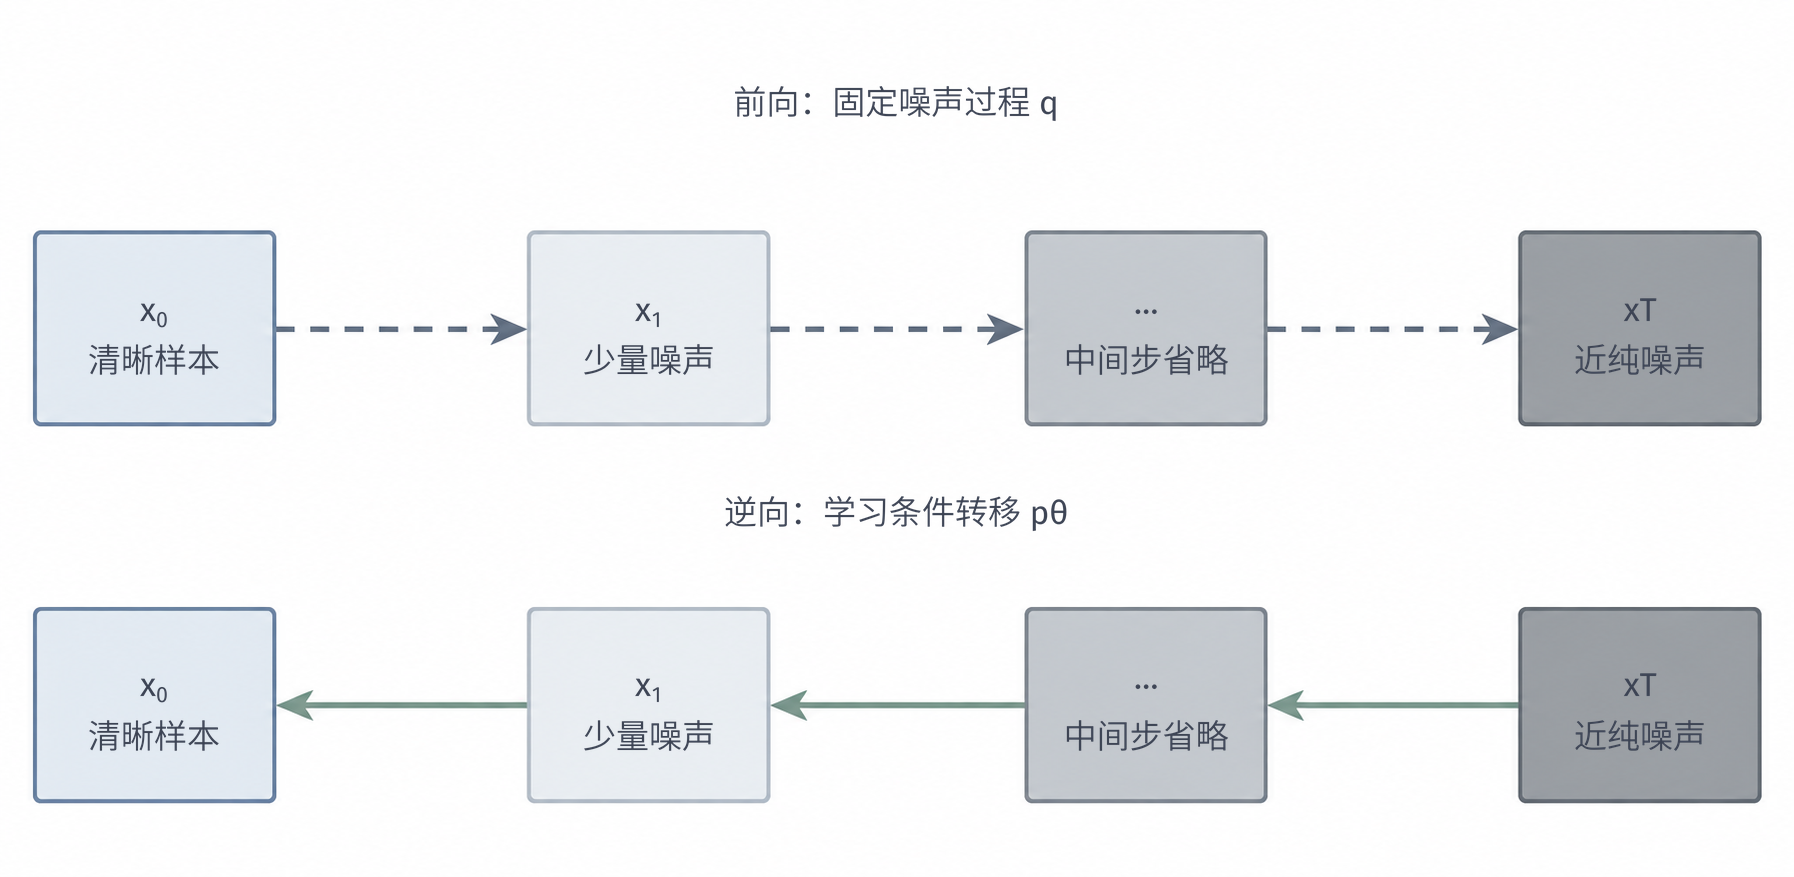
\includegraphics[width=112.000mm]{figures/06-probabilistic-graphical-models/04-models/generated/pgm-generative-diffusion/figure.png}
  \caption{离散扩散的前向扰动与逆向生成。上行按固定日程逐步加噪，下行从终端先验开始执行学得的逆转移。灰度与文字表示状态的噪声程度，相同下标对应相同噪声尺度。两行分别抽样；有限步下的终点匹配由日程和数据尺度决定。}
  \label{fig:pgm-generative-diffusion}
\end{figure}

图~\ref{fig:pgm-generative-diffusion}中的模型逆转移通常采用神经网络参数化的高斯均值与方差。真实逆转移$q(\bm{x}_{t-1}\mid\bm{x}_t)$还需对未知原观测混合，一般具有更复杂的分布形状。下面的解析高斯则额外给定原观测，描述$q(\bm{x}_{t-1}\mid\bm{x}_t,\bm{x}_0)$。因此，小步高斯是有限步模型的参数化选择，其逼近误差需要与原观测已知时的解析计算区分。

图~\ref{fig:diffusion-sample-process-illustration}通过样本插画表示噪声尺度的变化。下行以独立终端噪声启动学得的生成链，上行则由给定样本启动固定扰动链。

\begin{figure*}[htbp]
  \centering
  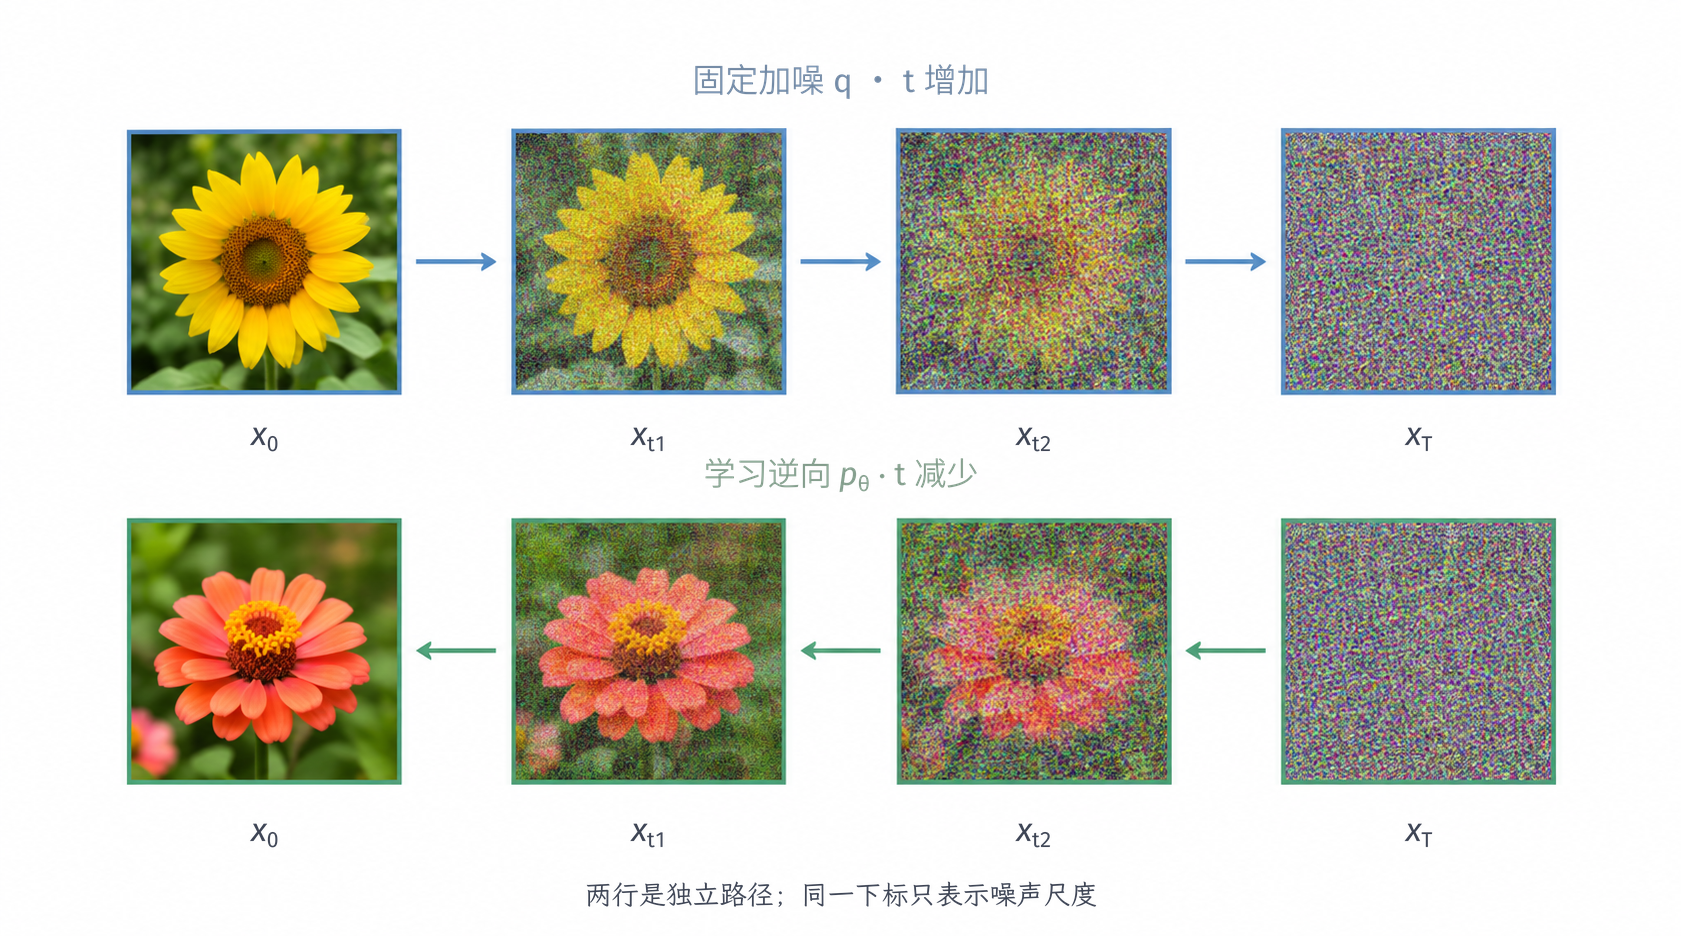
\includegraphics[width=139.534mm]{figures/06-probabilistic-graphical-models/04-models/generated/diffusion-sample-process-illustration/figure.png}
  \caption{扩散链的样本变化示意。上行从左向右逐步扰动观测，下行从右侧独立终端噪声开始向左生成；下标记录噪声尺度。花朵及中间状态为机制插画，用于说明扰动与生成方向。}
  \label{fig:diffusion-sample-process-illustration}
\end{figure*}

\subsection{变分目标与分数匹配}
\label{sec:pgm-generative-diffusion-objective}

逆向生成联合分布的学习可以采用路径变分下界。将观测固定为$\bm{x}_0$，以整条中间路径$\bm{x}_{1:T}$为潜变量，并用前向扰动分布作近似后验，一般ELBO便成为联合与前向路径密度比的期望（见式~\eqref{eq:pgm-variational-elbo}）。记路径下界为$\mathcal{B}_{\mathrm{diff}}(\bm{x}_0)$，其负值为$\mathcal{J}_{\mathrm{diff}}=-\mathcal{B}_{\mathrm{diff}}$：
\begin{equation}
  \label{eq:pgm-generative-path-elbo}
  \begin{aligned}
    \log p_{\bm{\theta}}(\bm{x}_0)
      &\geq\mathcal{B}_{\mathrm{diff}}(\bm{x}_0),\\
    \mathcal{J}_{\mathrm{diff}}(\bm{x}_0)
      &=\mathbb{E}_{q(\bm{x}_{1:T}\mid\bm{x}_0)}
         \left[\log
           \frac{q(\bm{x}_{1:T}\mid\bm{x}_0)}
                {p_{\bm{\theta}}(\bm{x}_{0:T})}
         \right].
  \end{aligned}
\end{equation}

要把这个路径比值化为局部计算，使用$t\geq2$时的Bayes恒等式
\[
  q(\bm{x}_t\mid\bm{x}_{t-1})
  =q(\bm{x}_{t-1}\mid\bm{x}_t,\bm{x}_0)
     \frac{q(\bm{x}_t\mid\bm{x}_0)}
          {q(\bm{x}_{t-1}\mid\bm{x}_0)}.
\]
将该恒等式代入前向路径密度，相邻边缘比值消去，得到同一路径密度的反向分解：
\[
  \begin{aligned}
    q(\bm{x}_{1:T}\mid\bm{x}_0)
      ={}&q(\bm{x}_T\mid\bm{x}_0)\\
         &{}\times\prod_{t=2}^{T}
              q(\bm{x}_{t-1}\mid\bm{x}_t,\bm{x}_0).
  \end{aligned}
\]
再对每个中间变量取条件期望，路径目标便分解为可局部评价的项：
\begin{equation}
  \label{eq:pgm-generative-ddpm-kl}
  \begin{aligned}
    \mathcal{J}_{\mathrm{diff}}(\bm{x}_0)
      ={}&\operatorname{KL}\bigl(
          q(\bm{x}_T\mid\bm{x}_0)\,\|\,p(\bm{x}_T)\bigr)\\
       &+\sum_{t=2}^{T}
         \mathbb{E}_{q(\bm{x}_t\mid\bm{x}_0)}
          \operatorname{KL}\bigl(
           q(\bm{x}_{t-1}\mid\bm{x}_t,\bm{x}_0)
           \,\|\,p_{\bm{\theta}}(\bm{x}_{t-1}\mid\bm{x}_t)
                         \bigr)\\
       &-\mathbb{E}_{q(\bm{x}_1\mid\bm{x}_0)}
          \log p_{\bm{\theta}}(\bm{x}_0\mid\bm{x}_1).
  \end{aligned}
\end{equation}

三部分分别评价终点匹配、逐步逆转移匹配和观测解码。固定日程与先验后，终点项与学习参数无关，求梯度时可以省略，报告完整似然界时仍计入其值。解码项评价已知观测的条件对数似然；它与中间变量的高斯KL具有不同形式，因为原观测在此已经固定。

给定原观测后，前向过程中的高斯结构使中间KL具有解析形式。对$t\geq2$，将$q(\bm{x}_t\mid\bm{x}_{t-1})q(\bm{x}_{t-1}\mid\bm{x}_0)$按待求中间变量配平方，二次项的精度系数为
\[
  \frac{\alpha_t}{\beta_t}
    +\frac{1}{1-\bar{\alpha}_{t-1}}
  =\frac{1-\bar{\alpha}_t}
          {\beta_t(1-\bar{\alpha}_{t-1})}.
\]
线性项为$\sqrt{\alpha_t}\bm{x}_t/\beta_t+\sqrt{\bar{\alpha}_{t-1}}\bm{x}_0/(1-\bar{\alpha}_{t-1})$。精度的倒数给出方差，方差与线性项相乘给出均值，因此条件分布为
\begin{equation}
  \label{eq:pgm-generative-forward-posterior}
  \begin{aligned}
    q(\bm{x}_{t-1}\mid\bm{x}_t,\bm{x}_0)
      &=\mathcal{N}(\bm{x}_{t-1};
          \widetilde{\bm{\mu}}_t,\widetilde{\beta}_t\bm{I}_d),\\
    \widetilde{\beta}_t
      &=\frac{\beta_t(1-\bar{\alpha}_{t-1})}
              {1-\bar{\alpha}_t},\\
    \widetilde{\bm{\mu}}_t
      &=\frac{\sqrt{\bar{\alpha}_{t-1}}\beta_t}
               {1-\bar{\alpha}_t}\bm{x}_0
       +\frac{\sqrt{\alpha_t}(1-\bar{\alpha}_{t-1})}
               {1-\bar{\alpha}_t}\bm{x}_t.
  \end{aligned}
\end{equation}
训练观测已知，可以直接计算这一条件均值作为监督目标。生成时只能使用当前状态、噪声步和给定外部条件，因此模型需要学习从这些输入预测相应均值。

现固定逆转移方差$\sigma_t^2>0$，令$p_{\bm{\theta}}(\bm{x}_{t-1}\mid\bm{x}_t)=\mathcal{N}(\bm{\mu}_{\bm{\theta}}(\bm{x}_t,t),\sigma_t^2\bm{I}_d)$。高斯KL分为均值误差与方差误差：
\begin{equation}
  \label{eq:pgm-generative-gaussian-step-kl}
  \begin{aligned}
    \operatorname{KL}(q\,\|\,p_{\bm{\theta}})
      &=\frac{\lVert\widetilde{\bm{\mu}}_t
                    -\bm{\mu}_{\bm{\theta}}(\bm{x}_t,t)\rVert_2^2}
               {2\sigma_t^2}+C_t,\\
    C_t&=\frac{d}{2}
       \left(\frac{\widetilde{\beta}_t}{\sigma_t^2}
              -1+\log\frac{\sigma_t^2}{\widetilde{\beta}_t}\right).
  \end{aligned}
\end{equation}
固定逆转移方差时，方差项$C_t$与待学习参数无关，常用选择为$\sigma_t^2=\beta_t$或在$t\geq2$时取$\sigma_t^2=\widetilde{\beta}_t$。逆转移方差参与学习时，均值误差权重与方差项都随参数变化，需要共同优化。若逆转移方差依赖当前状态而无待学习参数，方差项仍可在求梯度时省略，其数值则同时依赖状态与噪声步。

利用式~\eqref{eq:pgm-generative-forward-marginal}把$\bm{x}_0$换成$\bm{x}_t$和噪声，后验均值也可写成
\[
  \widetilde{\bm{\mu}}_t
  =\frac{1}{\sqrt{\alpha_t}}
       \left(\bm{x}_t-
          \frac{\beta_t}{\sqrt{1-\bar{\alpha}_t}}\bm{\epsilon}\right).
\]
该形式将均值学习转换为合成噪声预测。用网络$\bm{\epsilon}_{\bm{\theta}}(\bm{x}_t,t)$预测噪声，并据此定义模型均值：
\begin{equation}
  \label{eq:pgm-generative-noise-parameterization}
  \bm{\mu}_{\bm{\theta}}(\bm{x}_t,t)
  =\frac{1}{\sqrt{\alpha_t}}
       \left(\bm{x}_t-
          \frac{\beta_t}{\sqrt{1-\bar{\alpha}_t}}
               \bm{\epsilon}_{\bm{\theta}}(\bm{x}_t,t)\right).
\end{equation}
回到仅随噪声步变化的固定逆转移方差设定，两均值相减时$\bm{x}_t$项抵消。记$\ell_t(\bm{\theta})$为第$t$个中间KL的数据与扰动平均，并仍按式~\eqref{eq:pgm-generative-forward-marginal}抽取$\bm{x}_t$，则
\begin{equation}
  \label{eq:pgm-generative-weighted-denoising}
  \begin{aligned}
    \ell_t(\bm{\theta})
      &=w_t\,\mathbb{E}_{\bm{x}_0,\bm{\epsilon}}
         \lVert\bm{\epsilon}
          -\bm{\epsilon}_{\bm{\theta}}(\bm{x}_t,t)\rVert_2^2+C_t,\\
    w_t&=\frac{\beta_t^2}
              {2\sigma_t^2\alpha_t(1-\bar{\alpha}_t)},
          \qquad t=2,\ldots,T.
  \end{aligned}
\end{equation}
这一权重由固定逆转移方差下的高斯KL推导而来，通常随噪声步变化，因此决定不同噪声尺度对ELBO学习的相对贡献。

\begin{example}[核对一个扩散步的权重]
  \label{ex:pgm-generative-step-weight}
  取便于手算的噪声系数$\beta_1=0.2$、$\beta_2=0.25$，于是$\alpha_2=0.75$、$\bar{\alpha}_1=0.8$、$\bar{\alpha}_2=0.6$。在$t=2$时，给定原观测的条件方差为$\widetilde{\beta}_2=0.25(0.2)/0.4=0.125$。若模型逆转移方差取$\sigma_2^2=0.25$，去噪权重为$w_2=0.25^2/(2\cdot0.25\cdot0.75\cdot0.4)=5/12$。一维噪声预测误差取$0.3$，对应均值差的平方为
  \[
    \frac{0.25^2}{0.75\cdot0.4}(0.3)^2=0.01875,
  \]
  除以$2\sigma_2^2=0.5$得到$0.0375$，与$(5/12)(0.3)^2$一致。再加方差项$C_2=\tfrac12(0.5-1+\log2)\approx0.09657$，便得到完整KL。本例用较大的噪声系数核对均值参数化与去噪权重的代数关系。
\end{example}

DDPM还常用均匀抽步的噪声平方回归作为简化目标。独立抽取$t\sim\operatorname{Unif}\{1,\ldots,T\}$、$\bm{x}_0\sim p_{\mathrm{data}}$和$\bm{\epsilon}\sim\mathcal{N}(\bm{0},\bm{I}_d)$，定义
\begin{equation}
  \label{eq:pgm-generative-simple-loss}
  \mathcal{J}_{\mathrm{simple}}
  =\mathbb{E}_{t,\bm{x}_0,\bm{\epsilon}}
      \lVert\bm{\epsilon}
       -\bm{\epsilon}_{\bm{\theta}}(\bm{x}_t,t)\rVert_2^2.
\end{equation}
该目标为所有噪声步采用相同回归权重，并在$t=1$继续预测噪声。它改变了原ELBO中各尺度的权衡，报告似然下界时需回到完整路径目标。原始DDPM对离散像素以量化区间积分定义解码质量；连续数据采用固定方差高斯解码时，解码负对数似然则包含特定权重的平方误差及常数项。因此，简化噪声损失与这些解码项、逐步加权KL的数值不同\scite{pgm-generative-ho2020}

严格ELBO也可以通过随机抽步优化。对中间步按正概率$\pi_t$抽取$t\in\{2,\ldots,T\}$，用$w_t\lVert\bm{\epsilon}-\bm{\epsilon}_{\bm{\theta}}\rVert_2^2/\pi_t$无偏估计其中依赖参数的求和，并单独计算解码项。均匀抽步时，校正因子为中间步数；报告完整界值还需计入方差常数和终点项。

抽步概率的改变配合重要性校正，可以调整估计方差而保留原目标。直接改变步权重则调整训练准则。若模型表达能力不受限、各尺度可独立拟合，任意正权重都保留逐尺度平方回归的最优条件均值；有限共享网络需在不同尺度间分配容量，权重因而影响实际拟合结果。

噪声回归还可以理解为密度梯度学习。记前向扰动后的边缘密度为$q_t(\bm{x})$，其\term{分数}（score）$\bm{s}_t^*(\bm{x})=\nabla_{\bm{x}}\log q_t(\bm{x})$给出对数密度局部增加的方向。本章用$q_t$与前向路径记号保持一致，分数模型文献也常将该边缘记为$p_t$。虽然边缘分数未知，高斯扰动的条件分数可以直接计算：
\[
  \nabla_{\bm{x}_t}\log q(\bm{x}_t\mid\bm{x}_0)
  =-\frac{\bm{x}_t-\sqrt{\bar{\alpha}_t}\bm{x}_0}
           {1-\bar{\alpha}_t}
  =-\frac{\bm{\epsilon}}{\sqrt{1-\bar{\alpha}_t}}.
\]
若可以交换微分与积分，对$q_t(\bm{x}_t)=\int q(\bm{x}_t\mid\bm{x}_0)p_{\mathrm{data}}(\bm{x}_0)\,\mathrm{d}\bm{x}_0$求导并除以$q_t(\bm{x}_t)>0$，得到
\begin{equation}
  \label{eq:pgm-generative-denoising-identity}
  \bm{s}_t^*(\bm{x}_t)
  =\mathbb{E}\!\left[
       \nabla_{\bm{x}_t}\log q(\bm{x}_t\mid\bm{X}_0)
       \mid\bm{x}_t\right]
  =-\frac{\mathbb{E}[\bm{\epsilon}\mid\bm{x}_t]}
            {\sqrt{1-\bar{\alpha}_t}}.
\end{equation}
平方回归的总体最优预测为条件均值。因此，令$\bm{s}_{\bm{\theta}}=-\bm{\epsilon}_{\bm{\theta}}/\sqrt{1-\bar{\alpha}_t}$，噪声预测对应各尺度边缘分数的估计。给定受扰动状态后，多种原观测与噪声都可能产生它，回归目标中的随机噪声通过条件平均形成可预测部分。

\term{去噪分数匹配}（denoising score matching, DSM）以已知扰动核的条件分数训练未知边缘分数。令$\bm{a}=\nabla_{\bm{x}_t}\log q(\bm{x}_t\mid\bm{X}_0)$；在平方矩有限时，条件期望的正交分解把训练误差写为
\begin{equation}
  \label{eq:pgm-generative-dsm-decomposition}
  \mathbb{E}\lVert\bm{s}_{\bm{\theta}}-\bm{a}\rVert_2^2
  =\mathbb{E}\lVert\bm{s}_{\bm{\theta}}-\bm{s}_t^*\rVert_2^2
   +\mathbb{E}\lVert\bm{a}-\bm{s}_t^*\rVert_2^2.
\end{equation}
最后一项与网络参数无关，因此最小化条件分数误差等价于最小化边缘分数误差。对当前高斯核，噪声平方误差为条件分数平方误差乘以$(1-\bar{\alpha}_t)$。简化噪声损失与严格ELBO因而对应不同的DSM尺度加权，只有从指定生成模型推导的权重及其余项才组成该模型的ELBO。连续时间分数建模将这些噪声尺度连接起来\scite{pgm-generative-song2021}

把式~\eqref{eq:pgm-generative-noise-parameterization}改用分数表示，还得到
\[
  \bm{\mu}_{\bm{\theta}}(\bm{x}_t,t)
    =\frac{\bm{x}_t+\beta_t\bm{s}_{\bm{\theta}}(\bm{x}_t,t)}
            {\sqrt{\alpha_t}}.
\]
使用真分数时，该式给出真实逆转移的条件均值；转移的完整形状仍由数据分布决定。式~\eqref{eq:pgm-generative-gaussian-diffusion}的一维例子给出真分数$-x_t/(1+4\bar{\alpha}_t)$，代入即可核对均值。

分数也联系能量模型：若$q_t(\bm{x})\propto\exp[-E_t(\bm{x})]$，则$\bm{s}_t^*=-\nabla E_t$，因为归一化常数对空间求导后消失（见第~\ref{chap:pgm-energy-models}章）。一般向量网络近似分数时，还需额外条件才能把它表示为标量能量的梯度；直接评价归一化密度也需要相应密度构造。

算法~\ref{alg:pgm-generative-ddpm}采用连续观测，逆转移方差均预先固定且为正。全部转移均值由噪声网络按式~\eqref{eq:pgm-generative-noise-parameterization}计算，包括$t=1$的高斯解码分布$p_{\bm{\theta}}(\bm{x}_0\mid\bm{x}_1)$。同一噪声损失因而训练各步均值，解码阶段使用这组共享参数。

\begin{algorithm}[固定方差DDPM的学习与祖先采样]
  \label{alg:pgm-generative-ddpm}
  \begin{algorithmic}[1]
    \Require 连续观测数据集、固定$\beta_{1:T}$及正的逆转移方差$\sigma_{1:T}^2$
    \Ensure 学得的噪声网络与模型样本
    \State 初始化$\bm{\theta}$，预计算$\alpha_t,\bar{\alpha}_t$
    \For{每个训练小批量，直至停止条件满足}
      \State 为每个观测抽$t\sim\operatorname{Unif}\{1,\ldots,T\}$和标准高斯$\bm{\epsilon}$
      \State 按式~\eqref{eq:pgm-generative-forward-marginal}计算$\bm{x}_t$
      \State 由式~\eqref{eq:pgm-generative-simple-loss}更新参数
    \EndFor
    \State 抽$\bm{x}_T\sim\mathcal{N}(\bm{0},\bm{I}_d)$
    \For{$t=T,T-1,\ldots,2$}
      \State 用噪声网络和式~\eqref{eq:pgm-generative-noise-parameterization}计算$\bm{\mu}_{\bm{\theta}}$
      \State 独立抽$\bm{\xi}_t\sim\mathcal{N}(\bm{0},\bm{I}_d)$，令$\bm{x}_{t-1}=\bm{\mu}_{\bm{\theta}}+\sigma_t\bm{\xi}_t$
    \EndFor
    \State 抽$\bm{x}_0\sim p_{\bm{\theta}}(\bm{x}_0\mid\bm{x}_1)$并返回
  \end{algorithmic}
\end{algorithm}

算法采用简化训练损失。严格变分学习可将训练步骤替换为带权中间项估计和解码负对数似然。连续高斯解码的末步方差需单独指定正值，因为解析前向后验的$\widetilde{\beta}_1=0$对应已固定的原观测。末步也可以约定输出预测均值，但这种输出省去了正方差解码分布的随机波动。

设一次网络前向代价为$C_{\mathrm{net}}$，随机抽步训练的单样本前向代价约为$O(C_{\mathrm{net}}+d)$，完整祖先采样则为$O(T(C_{\mathrm{net}}+d))$。采样只需保留当前状态；评价全路径变分界还需处理全部项，或采用带校正的随机估计。训练抽步的计算收益因此与多步生成的成本并存。

\subsection{连续时间表示与采样}
\label{sec:pgm-generative-continuous-diffusion}

细化噪声步后，可以用连续索引$t\in[0,T_{\mathrm{c}}]$描述扰动，$T_{\mathrm{c}}$为终点。本节采用扩散系数仅依赖时间的各向同性设定，使逆向公式具有明确的分数项。设$\bm{W}_t$为$d$维标准\term{布朗运动}（Brownian motion），其不相交区间增量相互独立，长度$\Delta t$的增量服从$\mathcal{N}(\bm{0},\Delta t\,\bm{I}_d)$。前向\term{随机微分方程}（stochastic differential equation, SDE）为
\begin{equation}
  \label{eq:pgm-generative-forward-sde}
  \mathrm{d}\bm{X}_t
  =\bm{b}(\bm{X}_t,t)\,\mathrm{d}t
    +g(t)\,\mathrm{d}\bm{W}_t,
  \qquad \bm{X}_0\sim p_{\mathrm{data}}.
\end{equation}
漂移$\bm{b}$规定确定性的局部移动，$g(t)>0$规定噪声强度。为保证前向解存在且不爆炸，假设系数连续，漂移对空间全局Lipschitz且至多线性增长，噪声系数有界并在所讨论闭区间上有正下界。

使用反向密度公式还需密度和逆过程的正则性：假设$q_t>0$，对时间一阶、对空间二阶连续可微，所用时间区间上$\int\mathbb{E}_{q_t}\lVert\nabla\log q_t(\bm{X}_t)\rVert_2^2\,\mathrm{d}t<\infty$，且反向方程存在不爆炸的解。数据分布本身奇异时，可将这些条件限定于$t\geq\delta>0$的已加噪区间，观测端点另行处理。

与离散DDPM相应的方差保持过程采用$\bm{b}(\bm{x},t)=-\tfrac12\beta(t)\bm{x}$和$g(t)=\sqrt{\beta(t)}$。条件均值的衰减系数为$\exp[-\tfrac12\int_0^t\beta(s)\,\mathrm{d}s]$，条件方差为$1-\exp[-\int_0^t\beta(s)\,\mathrm{d}s]$。有限终点内的累计噪声积分有限时，仍有一部分原信号保留；终点与标准高斯的匹配需要通过累计扰动强度控制。

条件扰动核可解析时，可以从连续区间抽取噪声尺度，构造受扰动观测，再拟合条件分数$\nabla_{\bm{x}_t}\log q(\bm{x}_t\mid\bm{x}_0)$。式~\eqref{eq:pgm-generative-denoising-identity}和式~\eqref{eq:pgm-generative-dsm-decomposition}在满足条件的每个正噪声尺度上继续说明其边缘分数含义。时间抽样密度与损失权重共同决定训练比重；观测似然评价则需要后文的密度构造与积分计算。

记真分数为$\bm{s}_t^*=\nabla_{\bm{x}}\log q_t$。在上述正则条件及反向过程存在的设定下，反向SDE可以沿同一个$t$写成
\begin{equation}
  \label{eq:pgm-generative-reverse-sde}
  \begin{aligned}
    \mathrm{d}\bm{X}_t
    ={}&\bigl[\bm{b}(\bm{X}_t,t)-g(t)^2\bm{s}_t^*(\bm{X}_t)\bigr]
         \,\mathrm{d}t\\
       &+g(t)\,\mathrm{d}\overline{\bm{W}}_t,
    \qquad t:T_{\mathrm{c}}\downarrow0.
  \end{aligned}
\end{equation}
该式沿递减时间积分，$\mathrm{d}t<0$，反向布朗增量的协方差为$|\mathrm{d}t|\bm{I}_d$。实现时可改用递增反向索引$u=T_{\mathrm{c}}-t$，令$\bm{Y}_u=\bm{X}_{T_{\mathrm{c}}-u}$，将时间方向显式写入漂移：
\begin{equation}
  \label{eq:pgm-generative-positive-reverse-time}
  \begin{aligned}
    \mathrm{d}\bm{Y}_u
      ={}&-\bm{b}(\bm{Y}_u,T_{\mathrm{c}}-u)\,\mathrm{d}u\\
         &+g(T_{\mathrm{c}}-u)^2
              \bm{s}_{T_{\mathrm{c}}-u}^*(\bm{Y}_u)\,\mathrm{d}u\\
         &+g(T_{\mathrm{c}}-u)\,\mathrm{d}\bm{B}_u.
  \end{aligned}
\end{equation}
其中$\bm{B}_u$为递增反向索引下的标准布朗运动。该路径反演结果使用真分数及上述正则条件，其证明依赖随机过程反演理论。分数SDE框架还讨论了状态相关扩散系数；相应逆漂移包含扩散矩阵的空间导数，需采用更一般的公式\scite{pgm-generative-song2021}

式~\eqref{eq:pgm-generative-positive-reverse-time}也给出明确的数值一步。令$t=T_{\mathrm{c}}-u$、$\Delta u>0$，用学得分数替代真分数的Euler--Maruyama更新为
\[
  \begin{aligned}
    \bm{y}_{u+\Delta u}
      ={}&\bm{y}_u-\bm{b}(\bm{y}_u,t)\Delta u\\
         &+g(t)^2\bm{s}_{\bm{\theta}}(\bm{y}_u,t)\Delta u
          +g(t)\sqrt{\Delta u}\,\bm{\xi},
  \end{aligned}
\]
每一步独立抽取$\bm{\xi}\sim\mathcal{N}(\bm{0},\bm{I}_d)$。递增反向索引下，分数项为正号，真分数使该部分漂移沿对数密度增加方向移动；式~\eqref{eq:pgm-generative-reverse-sde}则将相同方向放在负时间增量中。精确恢复前向数据分布需要真实终点分布、真分数和精确求解。实际生成中的终端先验近似、分数估计和离散积分分别产生不同误差。

真分数可得时，还可以用确定性流保持前向SDE的各时刻边缘密度。\term{概率流常微分方程}（probability flow ordinary differential equation, probability flow ODE）采用速度场
\begin{equation}
  \label{eq:pgm-generative-probability-flow}
  \frac{\mathrm{d}\bm{X}_t}{\mathrm{d}t}
     =\bm{v}^*(\bm{X}_t,t),
  \qquad
  \bm{v}^*(\bm{x},t)
     =\bm{b}(\bm{x},t)-\frac12g(t)^2\bm{s}_t^*(\bm{x}).
\end{equation}
概率流速度中的分数系数为逆SDE对应系数的一半。给定终点后，ODE轨迹由速度场确定，样本之间的随机性来自终点抽样。下面通过密度守恒说明这一系数。

前向SDE的Fokker--Planck方程描述边缘密度随时间的变化：
\[
  \partial_t q_t
    =-\nabla\cdot(\bm{b}q_t)+\tfrac12g(t)^2\Delta q_t.
\]
利用$q_t\bm{s}_t^*=\nabla q_t$以及$g$不依赖$\bm{x}$，右侧等于
\[
  -\nabla\cdot
       \left[\left(\bm{b}-\tfrac12g(t)^2\bm{s}_t^*\right)q_t\right],
\]
该表达式是速度场$\bm{v}^*$的连续性方程。在适当边界衰减、共同初始密度及密度方程唯一性条件下，两种过程因此具有相同的单时刻边缘。路径分布仍不同：SDE包含沿途随机增量，ODE在给定初始点后采用确定性轨迹。

使用学得分数时，令$\bm{v}_{\bm{\theta}}=\bm{b}-\tfrac12g^2\bm{s}_{\bm{\theta}}$，并指定可评价密度的终端先验$p_{T_{\mathrm{c}}}$。速度场若生成正反两向均存在的可微流，终端分布及逆流便定义ODE密度模型$p_{\bm{\theta}}^{\mathrm{ODE}}$。沿数据到终点的轨迹积分瞬时变量变换公式，可评价这个模型的密度：
\begin{equation}
  \label{eq:pgm-generative-ode-likelihood}
  \begin{aligned}
    \log p_{\bm{\theta}}^{\mathrm{ODE}}(\bm{x}_0)
       &=\log p_{T_{\mathrm{c}}}(\bm{x}_{T_{\mathrm{c}}})
          +\int_0^{T_{\mathrm{c}}}
            \nabla_{\bm{x}}\cdot
            \bm{v}_{\bm{\theta}}(\bm{x}_t,t)\,\mathrm{d}t,\\
    \frac{\mathrm{d}\bm{x}_t}{\mathrm{d}t}
       &=\bm{v}_{\bm{\theta}}(\bm{x}_t,t),
       \qquad \bm{x}_{t=0}=\bm{x}_0.
  \end{aligned}
\end{equation}
瞬时公式表示终点对数密度减去起点对数密度等于负散度积分。移项求起点密度后，式中的散度积分因此取正号。密度评价从数据积分到终点，生成则从终端先验反向积分；两者采用同一速度场。

例如一维速度$v(x,t)=ax$、$T_{\mathrm{c}}=1$、终端密度$\mathcal{N}(0,1)$时，$x_1=e^a x_0$，散度积分为$a$，所以
\[
  \log p^{\mathrm{ODE}}(x_0)
  =-\tfrac12\log(2\pi)-\tfrac12e^{2a}x_0^2+a.
\]
结果等于$\mathcal{N}(0,e^{-2a})$的对数密度。取$a=-\tfrac12\log5$即得到$\mathcal{N}(0,5)$，其中散度积分提供正确的归一化因子。该线性场例子用于核对ODE变量变换的积分方向，速度场由本例单独指定。

式~\eqref{eq:pgm-generative-ode-likelihood}评价的是指定速度场与终端先验所定义的ODE分布。使用近似分数时，同一网络驱动的随机SDE通常定义另一分布，有限步DDPM又由其离散转移定义边缘。因此，三者的似然比较需要先确定模型对象；同边缘结果适用于真分数、匹配终点和精确求解的设定。

密度数值评价沿轨迹计算散度。随机迹估计产生蒙特卡洛误差，有限容差求解器产生轨迹与积分误差，两项计算相互耦合；固定矩阵上的无偏迹估计只处理其中一项性质。减小求解器容差和增加迹样本分别针对数值积分与随机估计，分数偏差和终点失配仍需通过模型学习与日程选择处理。

若把观测端点截断到$\delta>0$，所评价的是截断模型在该噪声尺度的密度，观测空间的概率还需通过后续解码或近似确定。离散像素似然另涉及量化区间质量或去量化下界，比较时需统一预处理及测度。

采样成本可以用网络函数评价次数衡量：高阶ODE步骤可能调用网络多次，自适应求解器还可能拒绝试步。随机采样沿途引入噪声，确定性采样在固定终点后便于重复生成与编码；两者的质量需在相同网络、预算和评价准则下比较。减少数值步通常降低计算，同时改变离散化误差。对有限步DDPM，完整执行全部转移对应该离散模型的祖先采样，跳过转移则需另行评价近似误差。

\term{采样蒸馏}（sampling distillation）进一步用一个已训练采样器的多步输出监督另一个少步模型。渐进蒸馏可把两个确定性教师步骤压成一个学生步骤，重复这一过程降低生成时的函数评价次数\scite{pgm-generative-salimans2022}

蒸馏将部分生成计算转移到额外训练，并引入学生对教师映射的近似。学生若需要评价密度，还需给出自身的密度构造与求值机制；采用可逆映射时，可以通过相应的体积变化追踪密度。扩散索引始终表示人为噪声尺度；用于视频等真实时序数据时，可对整个序列或其潜表示加噪，真实时间与噪声尺度各自承担不同的索引角色。

\section{模型关系与比较}
\label{sec:pgm-generative-comparison}

\subsection{似然、后验与采样}
\label{sec:pgm-generative-likelihood-posterior-sampling}

完整观测密度、部分观测下的条件分布、潜变量后验和无条件样本，构成四种不同查询。Flow可直接评价完整密度，部分观测查询仍可能需要边缘积分；VAE编码器快速给出近似后验，其误差由后验族、共享映射和优化决定；DDPM训练可以随机抽步，祖先生成则按逆转移顺序执行。固定查询对象后，模型的计算优势才能直接比较。

\term{概率电路}（probabilistic circuit, PC）通过计算图的结构约束支持概率查询。叶节点表示可精确评价和边缘化的简单分布，和节点执行加权混合，乘积节点组合不同变量块。查询沿图中的加法与乘法传播，为完整密度和边缘概率提供另一种计算安排\scite{pgm-generative-choi2020}

一种充分设定是将归一化的叶分布逐层组合，并令和节点的权重非负且和为$1$。和节点的各个孩子涉及同一组变量，这一条件称为\term{光滑性}（smoothness），也称完备性。乘积节点的各个孩子涉及互不相交的变量组，这一条件称为\term{可分解性}（decomposability）。从叶向根归纳，加权和保持归一化，不相交变量块上的乘积也保持归一化。边缘化时，先在叶节点积分，再沿原图进行加法与乘法传播；可分解性使不同变量块的积分能够拆开。设电路边数为$m$、叶查询代价为常数，一次向上传播的代价为$O(m)$。条件化分母的边缘概率质量或密度为正时，条件分布由两个相应边缘量之比得到。

线性传播成本相对于给定电路大小而言；复杂分布可能需要很大的表示。MAP和边缘MAP包含最大化，对混合分量的求和与最大化如何交换另需结构条件，因此其计算要求与边缘概率不同。概率电路由此说明，支持完整密度评价和支持大量边缘查询需要不同的结构安排。表~\ref{tab:pgm-generative-model-comparison}按查询对象概括各机制。

\begin{table*}[htbp]
  \centering
  \small
  \begin{tabularx}{\linewidth}{@{}lXXX@{}}
    \toprule
    机制 & 完整观测的似然 & 潜变量与条件查询 & 典型采样代价与限制 \\
    \midrule
    自回归基线
      & 条件分解给出精确似然
      & 一般缺失坐标不一定能高效边缘化
      & 通常按坐标顺序生成；依赖排序 \\
    VAE
      & 通常优化ELBO，边缘似然需额外估计
      & 编码器给出近似后验
      & 先抽潜变量再解码；条件似然决定额外成本 \\
    离散层Flow
      & 逆变换与Jacobian可行时精确
      & 完整观测有唯一逆像；部分观测仍可能需积分
      & 逐层变换；自回归流有方向性成本 \\
    DDPM
      & 路径ELBO可估计；简化损失不是似然值
      & 固定前向路径充当变分分布
      & 多步随机转移；有限终点与参数化有误差 \\
    分数ODE
      & 散度积分定义ODE模型密度
      & 可逆流给出编码，不是随机路径后验
      & 数值积分；精度与函数评价次数相关 \\
    受约束概率电路
      & 可精确评价归一化密度或质量
      & 合适结构下可精确边缘化与条件查询
      & 结构化采样；表示规模可能很大 \\
    \bottomrule
  \end{tabularx}
  \caption{不同生成机制的查询与采样成本。“精确”表示相应模型的数学计算关系可以直接评价，实际实现仍有浮点误差；连续流和分数ODE另需数值积分，并可能使用随机迹估计。概率电路采用正文的光滑性、可分解性及归一化条件。}
  \label{tab:pgm-generative-model-comparison}
\end{table*}

似然比较需要相同观测表示、测度和预处理。样本中的任务结构、模式覆盖和生成成本则由相应指标分别评价。一维例子中的三种机制都可表达$\mathcal{N}(0,5)$，潜变量关系与生成路径却不同；仅凭观测边缘无法识别这些内部机制。

在表达能力方面，VAE的生成族、Flow的可逆结构和扩散的逆转移族分别限制候选分布。增加网络容量可以改善函数拟合，但Flow的支撑约束、VAE的条件似然假设及有限步高斯逆转移的形状限制仍取决于模型结构。

在收敛性方面，需要先确定优化目标：VAE优化下界，离散Flow直接优化似然，扩散可优化路径下界或尺度加权的去噪目标。非凸参数化、随机梯度、近似推断和数值求解分别影响能否达到目标最优值，以及所需迭代和每次迭代成本；下界变紧或回归误差下降本身只回答相应训练目标的改进。

在泛化性方面，训练找到的候选分布还需在未参与拟合、配置选择或停止位置选择的独立观测上评价。样本量与模式覆盖、候选族容量、参数约束和训练终止共同影响这种表现，数据采集分布的改变还会改变预测任务。留出似然或其明确的估计、任务样本质量和模式覆盖应分别报告；网络训练的收敛与泛化分析可参考\BookChapterRef{chap:neural-network-training}{卷5《模型：神经网络模型》第8章“神经网络的训练”}和\BookChapterRef{chap:neural-network-generalization}{卷5《模型：神经网络模型》第9章“神经网络的泛化”}。

\subsection{生成机制的组合}
\label{sec:pgm-generative-hybrids}

组合生成机制时，先确定被调整的概率对象。采用Flow后验扩大$q_{\bm{\phi}}(\bm{z}\mid\bm{x})$的表达范围，主要针对近似族误差。新族包含原族时，理论最优下界至少与原来相同，实际改善仍取决于优化。采用Flow先验则改变$p_{\bm{\theta}}(\bm{z})$，调整无条件生成时访问潜空间的方式。同类可逆网络因此可以承担推断和生成两种不同角色。

层次VAE通过多个随机潜变量层表示观测依赖。对于前文的两层例子，若取$q_{\bm{\phi}}(\bm{z}_1,\bm{z}_2\mid\bm{x})=q_{\bm{\phi}}(\bm{z}_1\mid\bm{x})q_{\bm{\phi}}(\bm{z}_2\mid\bm{z}_1,\bm{x})$，ELBO就是
\[
  \mathbb{E}_{q_{\bm{\phi}}}
  \left[
    \log\frac{
      p(\bm{z}_2)p_{\bm{\theta}}(\bm{z}_1\mid\bm{z}_2)
          p_{\bm{\theta}}(\bm{x}\mid\bm{z}_1)}
      {q_{\bm{\phi}}(\bm{z}_1\mid\bm{x})
          q_{\bm{\phi}}(\bm{z}_2\mid\bm{z}_1,\bm{x})}
  \right].
\]
下界继续采用生成联合与变分路径密度比的期望，可通过逐层抽样估计。每层后验都需与相应生成依赖匹配，层次模型因而仍存在推断误差和潜变量利用问题。扩散的多层潜状态还配有噪声尺度、固定前向核及专门的局部目标，这些安排决定了它与一般层次VAE的计算差异。

\term{潜空间扩散}（latent diffusion）把多步生成放在观测的潜表示中：先学习编码与解码，再在编码得到的潜变量分布上训练扩散模型，最后把生成的潜变量解码为观测。其主要计算收益来自反复去噪的空间更小；原始潜空间扩散工作在预训练自编码表示上构造这一过程\scite{pgm-generative-rombach2022}

若解码器是归一化条件分布$p_{\bm{\psi}}(\bm{x}\mid\bm{z})$，潜空间生成先验为$p_{\bm{\theta}}^{\mathrm{diff}}(\bm{z})$，整体模型为
\begin{equation}
  \label{eq:pgm-generative-latent-diffusion}
  p_{\bm{\theta},\bm{\psi}}(\bm{x})
  =\int p_{\bm{\psi}}(\bm{x}\mid\bm{z})
          p_{\bm{\theta}}^{\mathrm{diff}}(\bm{z})\,\mathrm{d}\bm{z}.
\end{equation}
整体观测密度仍由潜变量积分给出，其计算包含潜空间生成和条件解码两部分。非可逆确定性解码器或主要由感知损失训练的编码过程，需要另行规定观测空间的概率语义，才能评价像素似然。压缩造成的信息损失、潜空间分布的拟合误差和解码族限制分别作用于生成结果；组合收益需连同这些代价一起评价。

\subsection{与隐式生成模型的边界}
\label{sec:pgm-generative-implicit-boundary}

假设只给出$\bm{Z}\sim p_0$和生成程序$\bm{X}=G_{\bm{\theta}}(\bm{Z})$。对任意可测集合$B$，它已经规定
\begin{equation}
  \label{eq:pgm-generative-pushforward}
  \mathbb{P}_{\bm{\theta}}(\bm{X}\in B)
  =\int \mathbf{1}\{G_{\bm{\theta}}(\bm{z})\in B\}
           p_0(\bm{z})\,\mathrm{d}\bm{z}.
\end{equation}
这种通过采样程序间接规定的分布称为\term{隐式分布}（implicit distribution）。\term{生成对抗网络}（generative adversarial network, GAN）是常见例子：通常的生成器提供样本，却不提供像式~\eqref{eq:pgm-generative-flow-density}那样可直接评价的观测密度。这里将GAN作为通过生成程序定义分布的例子，相关比较针对密度与采样查询\scite{pgm-generative-goodfellow2014}

密度评价涉及逆像计算，也涉及采用的测度。同维光滑映射即使处处局部可逆，全局多对一时通常仍需累加所有逆像的贡献，普通网络未必支持枚举这些逆像。若基础变量维度低于观测维度，局部Lipschitz生成网络的输出还可能集中于低维集合，在整个观测空间的Lebesgue测度下没有密度。推送公式依然定义合法分布，相应查询需要采用适合该分布的概率表达。

Flow同样将噪声推送为观测，并进一步利用同维可逆变换和可计算体积因子评价密度。VAE与离散扩散则给出可评价的联合分布，把观测密度明确写为潜变量边缘积分，进而构造似然下界。生成程序、密度存在性、密度求值算法和下界估计因此对应不同性质；模型提供哪些查询，可由这些具体概率构造判断。

\section{本章小结}
\label{sec:pgm-generative-summary}

概率生成模型通过不同结构协调归一化、密度评价、推断和采样。VAE用潜变量边缘化定义观测密度，以近似后验和ELBO学习参数；规范化流为完整观测建立唯一逆像，用Jacobian追踪局部体积；扩散以人工噪声过程构造潜状态，通过局部去噪目标学习逆向生成。三种机制可以组合，也可以表达相同观测分布，其潜变量含义和查询成本仍各有差异。

训练目标由具体概率构造决定。VAE重构项来自观测似然，后验灵活性影响下界差距；DDPM路径ELBO由终点项、逐步加权KL和解码项组成，均匀噪声回归调整了尺度权衡。连续逆SDE需结合积分方向解释漂移符号，概率流ODE的同边缘结果使用真分数及匹配边界。ODE模型的密度评价另需散度积分，其实现同时受数值求解和随机迹估计影响。

选择模型时，所需查询确定评价重点：潜变量推断关注后验误差，完整密度评价关注逆变换或边缘积分，缺失变量查询关注边缘化结构，低延迟生成关注网络评价次数与顺序依赖。进一步分析表达能力、收敛性和泛化性，可以分别判断候选分布的限制、训练达到目标的条件与成本，以及新观测上的表现。样本质量与这些概率查询各自提供证据，共同说明模型在具体任务中的作用。

\paragraph{扩展阅读}
VAE原论文介绍近似后验与变分下界，Rezende与Mohamed讨论用可逆变换扩展变分后验，Sohl-Dickstein等介绍逐步噪声的生成过程。三项工作分别适合进一步考察后验近似、推断族表达能力和多步随机生成；阅读时可将密度求值与采样成本对应到各自的概率构造\scite{kingma2013,pgm-overview-rezende2015,pgm-overview-sohl2015}

